 
% easychair.tex,v 3.5 2017/03/15

\documentclass{easychair}
%\documentclass[EPiC]{easychair}
%\documentclass[EPiCempty]{easychair}
%\documentclass[debug]{easychair}
%\documentclass[verbose]{easychair}
%\documentclass[notimes]{easychair}
%\documentclass[withtimes]{easychair}
%\documentclass[a4paper]{easychair}
%\documentclass[letterpaper]{easychair}

\usepackage{pifont}
\usepackage{xcolor}
\usepackage{comment}

\definecolor{second}{HTML}{007000}

\usepackage{doc}

\usepackage{cite}

% pretty tables defined with data files
\usepackage{booktabs}
\usepackage{longtable}
\usepackage{pgfplotstable}
\usepackage{titlesec}
\usepackage{multirow}
\usepackage{subcaption}
\usepackage{fancyvrb}
\usepackage{cleveref}

\pgfplotsset{compat=1.16}


% long table macro for pgfplotstable
% see https://tex.stackexchange.com/questions/66504/pgfplotstable-longtable-with-caption-and-repeating-header
\pgfkeysifdefined{/pgfplots/table/output empty row/.@cmd}{
    % upcoming releases offer this more convenient option:
    \pgfplotstableset{
        empty header/.style={
          every head row/.style={output empty row},
        }
    }
}{
    % versions up to and including 1.5.1 need this:
    \pgfplotstableset{
        empty header/.style={
            typeset cell/.append code={%
                \ifnum\pgfplotstablerow=-1 %
                    \pgfkeyssetvalue{/pgfplots/table/@cell content}{}%
                \fi
            }
        }
    }
}
%%%-----------------------------------------------

% use this if you have a long article and want to create an index
% \usepackage{makeidx}

% In order to save space or manage large tables or figures in a
% landcape-like text, you can use the rotating and pdflscape
% packages. Uncomment the desired from the below.
%
% \usepackage{rotating}
% \usepackage{pdflscape}

% Some of our commands for this guide.
%
\newcommand{\easychair}{\textsf{easychair}}
\newcommand{\miktex}{MiK{\TeX}}
\newcommand{\texniccenter}{{\TeX}nicCenter}
\newcommand{\makefile}{\texttt{Makefile}}
\newcommand{\latexeditor}{LEd}

\newcommand{\todoForParticipants}[1]{\textcolor{red}{TODO-PARTICIPANTS: #1}}

\newcommand{\todo}[1]{\textcolor{red}{TODO: #1}}

\titlespacing*{\paragraph}
{0pt}{2pt}{5pt}
%\makeindex

%% Front Matter
%%
% Regular title as in the article class.
%
\title{The Fifth International Verification of Neural Networks Competition (VNN-COMP 2024): Summary and Results%
%\thanks{Other people who contributed to this document include Maria Voronkov   (Imperial College and EasyChair) and Graham Gough (The University of Manchester).}
}

% Authors are joined by \and. Their affiliations are given by \inst, which indexes
% into the list defined using \institute
%
\author{
    Stanley Bak\thanks{S. Bak is with Stony Brook University, \tt stanley.bak@stonybrook.edu.} \and
    Christopher Brix\thanks{C. Brix is with RWTH Aachen University, \tt brix@cs.rwth-aachen.de.} \and
    Taylor Johnson\thanks{T. Johnson is with Vanderbilt University, \tt taylor.johnson@vanderbilt.edu.} \and
    Changliu Liu\thanks{C. Liu is with Carnegie Mellon University, \tt cliu6@andrew.cmu.edu.} \and
    Andrew (Haoze) Wu\thanks{A. Wu is with Stanford University, \tt haozewu@stanford.edu.}
%Serguei A. Mokhov\inst{1}\thanks{Designed and implemented the class style}
%\and
%    Geoff Sutcliffe\inst{2}\thanks{Did numerous tests and provided a lot of suggestions}
%\and
%   Andrei Voronkov\inst{3}\inst{4}\inst{5}\thanks{Masterminded EasyChair and created versions
%     3.0--3.5 of the class style}
}

% Institutes for affiliations are also joined by \and,
\institute{
%  Concordia University,
%  Montreal, Quebec, Canada\\
%  \email{mokhov@cse.concordia.ca}
%\and
%   University of Miami,
%   Miami, Florida, U.S.A.\\
%   \email{geoff@cs.miami.edu}\\
%\and
%   University of Manchester,
%   Manchester, U.K.\\
%   \email{andrei@voronkov.com}\\
%\and
%   Chalmers University of Technology,
%   Gothenburg, Sweden
%\and
%   EasyChair
 }

%  \authorrunning{} has to be set for the shorter version of the authors' names;
% otherwise a warning will be rendered in the running heads. When processed by
% EasyChair, this command is mandatory: a document without \authorrunning
% will be rejected by EasyChair

\authorrunning{}
\date{\phantom{date}\\}
% \titlerunning{} has to be set to either the main title or its shorter
% version for the running heads. When processed by
% EasyChair, this command is mandatory: a document without \titlerunning
% will be rejected by EasyChair
\titlerunning{VNN-COMP 2024 Report}

\begin{document}

\maketitle

\begin{abstract}
This report summarizes the fifth International Verification of Neural Networks Competition (VNN-COMP 2024), held as a part of the 6th Workshop on Formal Methods for ML-Enabled Autonomous Systems (FoMLAS) that was collocated with the 35th International Conference on Computer-Aided Verification (CAV).
%
%Twelve teams participated in this competition.
%
The goal of the competition is to provide an objective comparison of the state-of-the-art methods in neural network verification, in terms of scalability and speed.
%
Along this line, we used standard formats (ONNX for neural networks and VNNLIB for specifications), standard hardware (all tools are run by the organizers on AWS), and tool parameters provided by the tool authors.
%
This report summarizes the rules, benchmarks, participating tools, results, and lessons learned from this competition.
\end{abstract}



%------------------------------------------------------------------------------
%\input{tables}
\section{Total Score}

%Total Score:

\begin{table}[h]
\begin{center}
\caption{Overall Score} \label{tab:score}
{\setlength{\tabcolsep}{2pt}
\begin{tabular}[h]{@{}lll@{}}
\toprule
\textbf{\# ~} & \textbf{Tool} & \textbf{Score}\\
\midrule
1 & $\alpha$-$\beta$-CROWN & 1600.0 \\
2 & NeuralSAT & 1360.1 \\
3 & PyRAT & 1218.5 \\
4 & CORA & 954.6 \\
5 & nnenum & 740.8 \\
6 & NNV & 697.3 \\
7 & SobolBox & 529.0 \\
\bottomrule
\end{tabular}
}
\end{center}
\end{table}



\begin{figure}[h]
\centerline{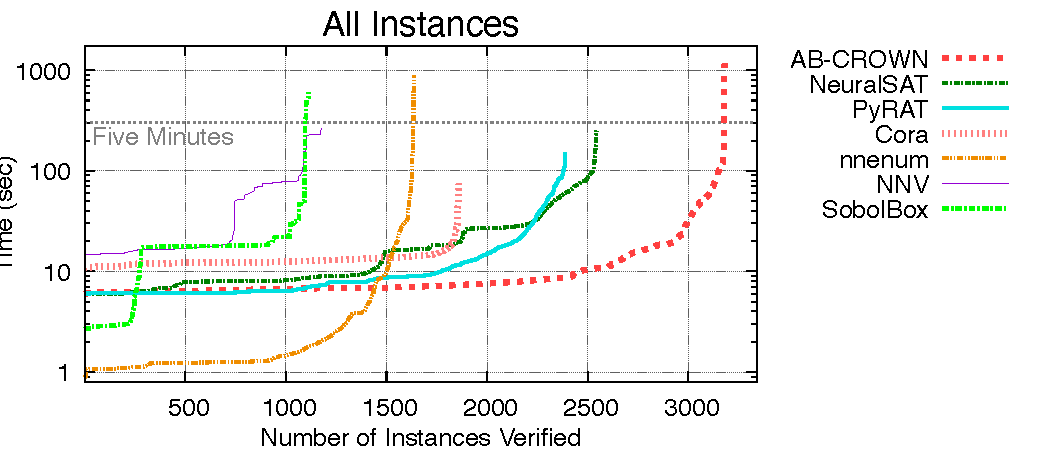
\includegraphics[width=\textwidth]{cactus/all.pdf}}
\caption{Cactus Plot for All Instances.}
\label{fig:quantPic}
\end{figure}


\begin{figure}[h]
\centerline{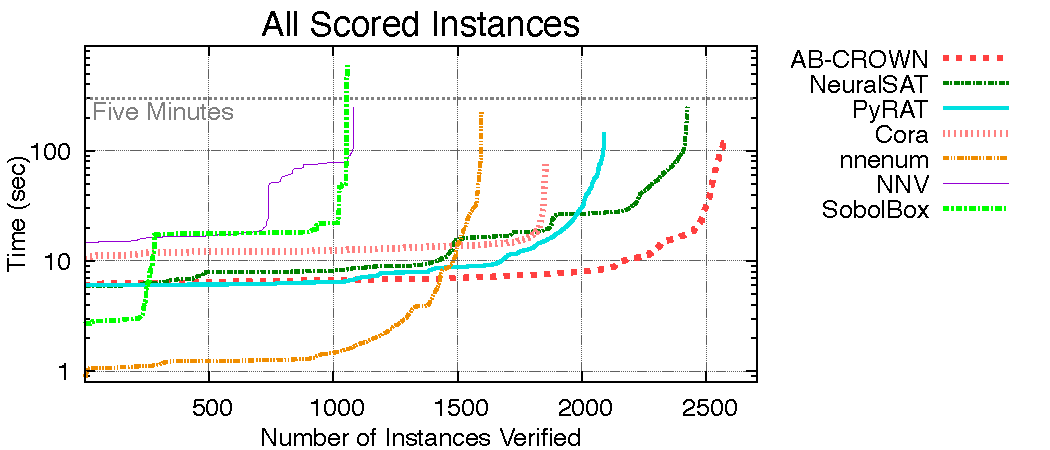
\includegraphics[width=\textwidth]{cactus/all_scored.pdf}}
\caption{Cactus Plot for All Scored Instances.}
\label{fig:quantPic}
\end{figure}





\clearpage
\section{Scored Benchmarks}

\clearpage
% Category 2025_acasxu_2023 (single_overhead=True):

\begin{table}[h]
\begin{center}
\caption{Benchmark \texttt{2025-acasxu-2023}} \label{tab:cat_2025_acasxu_2023}
{\setlength{\tabcolsep}{2pt}
\begin{tabular}[h]{@{}llllllrrr@{}}
\toprule
\textbf{\# ~} & \textbf{Tool} & \textbf{Verified} & \textbf{Falsified} & \textbf{Fastest} & \textbf{Penalty} & \textbf{Points} & \textbf{Score} & \textbf{Solved}\\
\midrule
1 & nnenum & 139 & 47 & 0 & 0 & 1860 & 100.0 & 100.0\% \\
2 & NeuralSAT & 139 & 47 & 0 & 0 & 1860 & 100.0 & 100.0\% \\
3 & $\alpha$-$\beta$-CROWN & 139 & 47 & 0 & 0 & 1860 & 100.0 & 100.0\% \\
4 & PyRAT & 139 & 46 & 0 & 0 & 1850 & 99.5 & 99.5\% \\
5 & CORA & 137 & 46 & 0 & 0 & 1830 & 98.4 & 98.4\% \\
6 & SobolBox & 118 & 43 & 0 & 1 & 1460 & 78.5 & 86.6\% \\
7 & NNV & 71 & 39 & 0 & 0 & 1100 & 59.1 & 59.1\% \\
\bottomrule
\end{tabular}
}
\end{center}
\end{table}



\begin{figure}[h]
\centerline{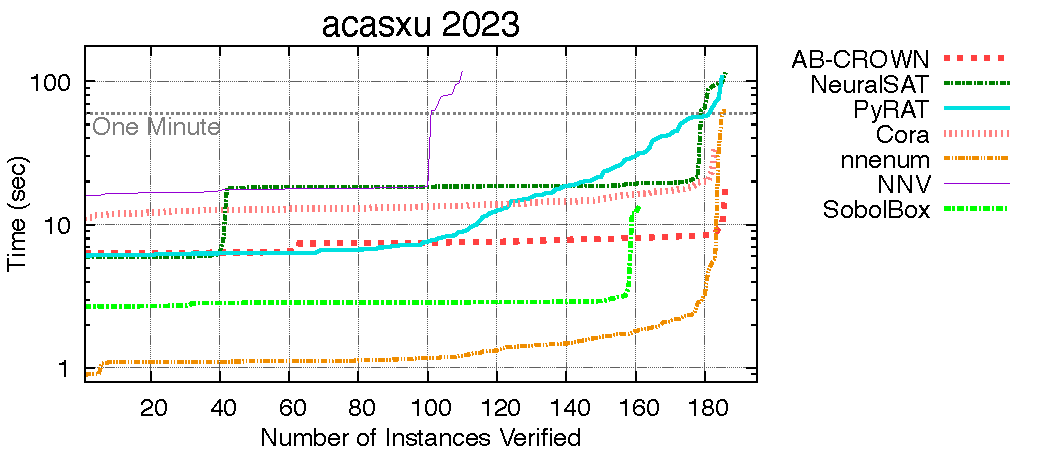
\includegraphics[width=\textwidth]{cactus/2025_acasxu_2023.pdf}}
\caption{Cactus Plot for acasxu 2023.}
\label{fig:quantPic}
\end{figure}


\clearpage
% Category 2025_cersyve (single_overhead=True):

\begin{table}[h]
\begin{center}
\caption{Benchmark \texttt{2025-cersyve}} \label{tab:cat_2025_cersyve}
{\setlength{\tabcolsep}{2pt}
\begin{tabular}[h]{@{}llllllrrr@{}}
\toprule
\textbf{\# ~} & \textbf{Tool} & \textbf{Verified} & \textbf{Falsified} & \textbf{Fastest} & \textbf{Penalty} & \textbf{Points} & \textbf{Score} & \textbf{Solved}\\
\midrule
1 & $\alpha$-$\beta$-CROWN & 6 & 6 & 0 & 0 & 120 & 100.0 & 100.0\% \\
2 & NeuralSAT & 4 & 6 & 0 & 0 & 100 & 83.3 & 83.3\% \\
3 & PyRAT & 2 & 6 & 0 & 0 & 80 & 66.7 & 66.7\% \\
4 & SobolBox & 0 & 6 & 0 & 0 & 60 & 50.0 & 50.0\% \\
5 & NNV & 0 & 3 & 0 & 0 & 30 & 25.0 & 25.0\% \\
6 & CORA & 6 & 5 & 0 & 1 & -40 & 0 & 91.7\% \\
\bottomrule
\end{tabular}
}
\end{center}
\end{table}



\begin{figure}[h]
\centerline{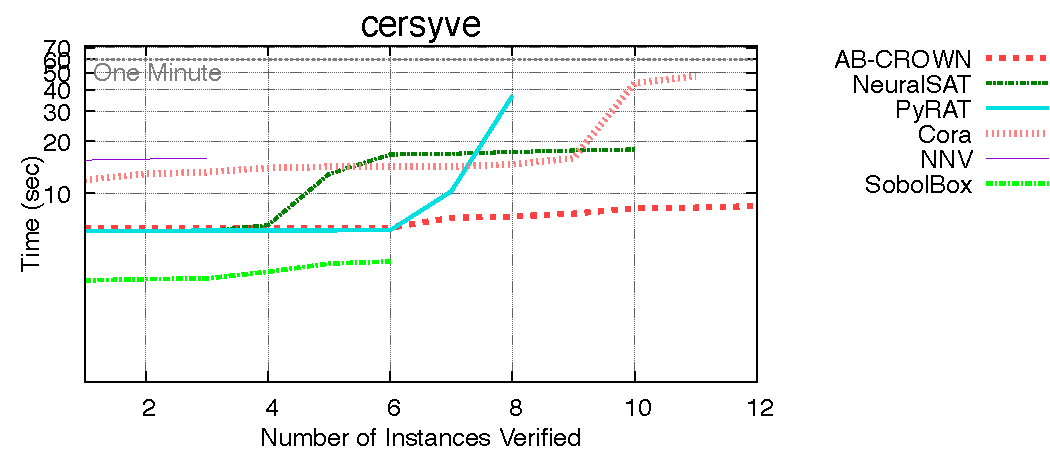
\includegraphics[width=\textwidth]{cactus/2025_cersyve.pdf}}
\caption{Cactus Plot for cersyve.}
\label{fig:quantPic}
\end{figure}


\clearpage
% Category 2025_cgan_2023 (single_overhead=True):

\begin{table}[h]
\begin{center}
\caption{Benchmark \texttt{2025-cgan-2023}} \label{tab:cat_2025_cgan_2023}
{\setlength{\tabcolsep}{2pt}
\begin{tabular}[h]{@{}llllllrrr@{}}
\toprule
\textbf{\# ~} & \textbf{Tool} & \textbf{Verified} & \textbf{Falsified} & \textbf{Fastest} & \textbf{Penalty} & \textbf{Points} & \textbf{Score} & \textbf{Solved}\\
\midrule
1 & PyRAT & 9 & 12 & 0 & 0 & 210 & 100.0 & 100.0\% \\
2 & NeuralSAT & 9 & 12 & 0 & 0 & 210 & 100.0 & 100.0\% \\
3 & $\alpha$-$\beta$-CROWN & 9 & 12 & 0 & 0 & 210 & 100.0 & 100.0\% \\
4 & SobolBox & 9 & 10 & 0 & 0 & 190 & 90.5 & 90.5\% \\
5 & nnenum & 7 & 10 & 0 & 0 & 170 & 81.0 & 81.0\% \\
6 & NNV & 5 & 11 & 0 & 0 & 160 & 76.2 & 76.2\% \\
\bottomrule
\end{tabular}
}
\end{center}
\end{table}



\begin{figure}[h]
\centerline{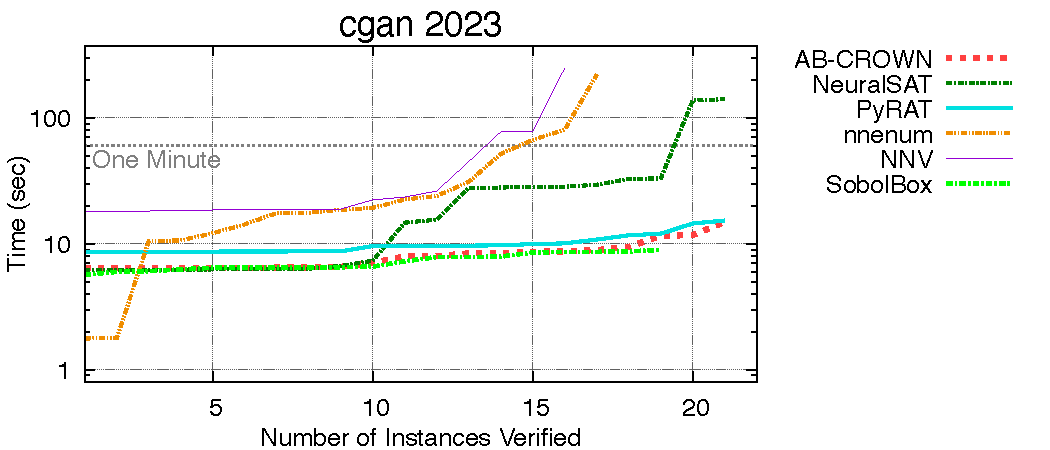
\includegraphics[width=\textwidth]{cactus/2025_cgan_2023.pdf}}
\caption{Cactus Plot for cgan 2023.}
\label{fig:quantPic}
\end{figure}


\clearpage
% Category 2025_cifar100_2024 (single_overhead=True):

\begin{table}[h]
\begin{center}
\caption{Benchmark \texttt{2025-cifar100-2024}} \label{tab:cat_2025_cifar100_2024}
{\setlength{\tabcolsep}{2pt}
\begin{tabular}[h]{@{}llllllrrr@{}}
\toprule
\textbf{\# ~} & \textbf{Tool} & \textbf{Verified} & \textbf{Falsified} & \textbf{Fastest} & \textbf{Penalty} & \textbf{Points} & \textbf{Score} & \textbf{Solved}\\
\midrule
1 & $\alpha$-$\beta$-CROWN & 100 & 29 & 0 & 0 & 1290 & 100.0 & 64.5\% \\
2 & PyRAT & 61 & 25 & 0 & 0 & 860 & 66.7 & 43.0\% \\
3 & NeuralSAT & 87 & 25 & 0 & 4 & 520 & 40.3 & 56.0\% \\
4 & CORA & 0 & 10 & 0 & 0 & 100 & 7.8 & 5.0\% \\
5 & NNV & 171 & 0 & 0 & 19 & -1140 & 0 & 85.5\% \\
\bottomrule
\end{tabular}
}
\end{center}
\end{table}



\begin{figure}[h]
\centerline{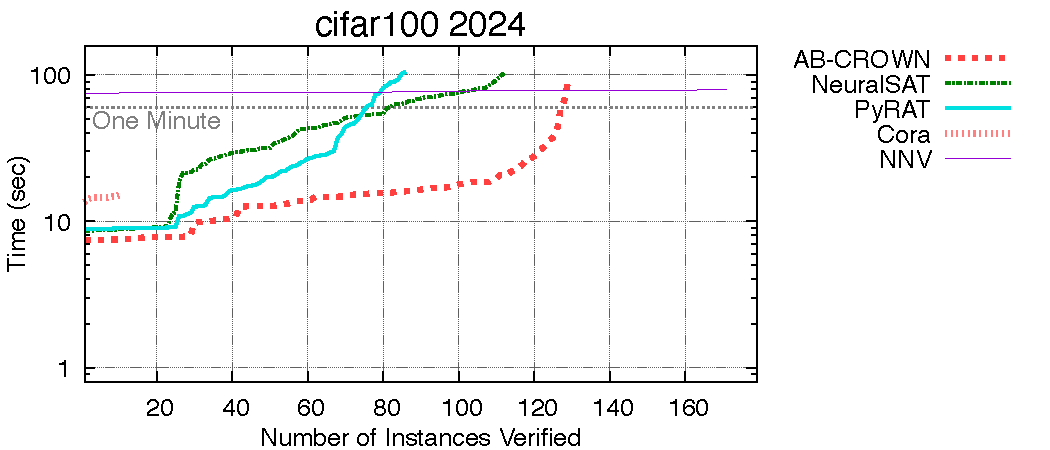
\includegraphics[width=\textwidth]{cactus/2025_cifar100_2024.pdf}}
\caption{Cactus Plot for cifar100 2024.}
\label{fig:quantPic}
\end{figure}


\clearpage
% Category 2025_collins_rul_cnn_2022 (single_overhead=True):

\begin{table}[h]
\begin{center}
\caption{Benchmark \texttt{2025-collins-rul-cnn-2022}} \label{tab:cat_2025_collins_rul_cnn_2022}
{\setlength{\tabcolsep}{2pt}
\begin{tabular}[h]{@{}llllllrrr@{}}
\toprule
\textbf{\# ~} & \textbf{Tool} & \textbf{Verified} & \textbf{Falsified} & \textbf{Fastest} & \textbf{Penalty} & \textbf{Points} & \textbf{Score} & \textbf{Solved}\\
\midrule
1 & nnenum & 39 & 23 & 0 & 0 & 620 & 100.0 & 100.0\% \\
2 & PyRAT & 39 & 23 & 0 & 0 & 620 & 100.0 & 100.0\% \\
3 & NeuralSAT & 39 & 23 & 0 & 0 & 620 & 100.0 & 100.0\% \\
4 & NNV & 39 & 23 & 0 & 0 & 620 & 100.0 & 100.0\% \\
5 & CORA & 39 & 23 & 0 & 0 & 620 & 100.0 & 100.0\% \\
6 & $\alpha$-$\beta$-CROWN & 39 & 23 & 0 & 0 & 620 & 100.0 & 100.0\% \\
7 & SobolBox & 19 & 15 & 0 & 0 & 340 & 54.8 & 54.8\% \\
\bottomrule
\end{tabular}
}
\end{center}
\end{table}



\begin{figure}[h]
\centerline{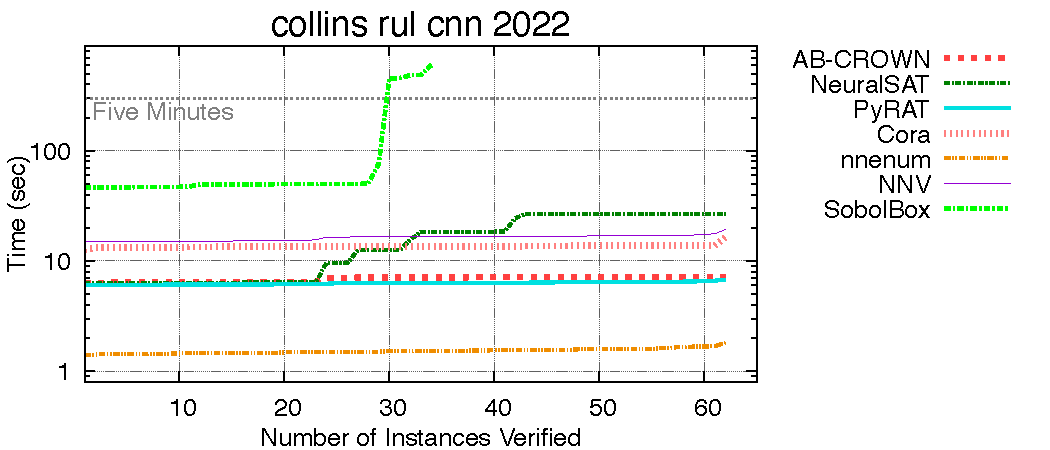
\includegraphics[width=\textwidth]{cactus/2025_collins_rul_cnn_2022.pdf}}
\caption{Cactus Plot for collins rul cnn 2022.}
\label{fig:quantPic}
\end{figure}


\clearpage
% Category 2025_cora_2024 (single_overhead=True):

\begin{table}[h]
\begin{center}
\caption{Benchmark \texttt{2025-cora-2024}} \label{tab:cat_2025_cora_2024}
{\setlength{\tabcolsep}{2pt}
\begin{tabular}[h]{@{}llllllrrr@{}}
\toprule
\textbf{\# ~} & \textbf{Tool} & \textbf{Verified} & \textbf{Falsified} & \textbf{Fastest} & \textbf{Penalty} & \textbf{Points} & \textbf{Score} & \textbf{Solved}\\
\midrule
1 & $\alpha$-$\beta$-CROWN & 22 & 131 & 0 & 0 & 1530 & 100.0 & 85.0\% \\
2 & NeuralSAT & 21 & 131 & 0 & 0 & 1520 & 99.3 & 84.4\% \\
3 & PyRAT & 20 & 128 & 0 & 0 & 1480 & 96.7 & 82.2\% \\
4 & CORA & 19 & 124 & 0 & 0 & 1430 & 93.5 & 79.4\% \\
5 & NNV & 19 & 57 & 0 & 0 & 760 & 49.7 & 42.2\% \\
6 & nnenum & 19 & 4 & 0 & 0 & 230 & 15.0 & 12.8\% \\
\bottomrule
\end{tabular}
}
\end{center}
\end{table}



\begin{figure}[h]
\centerline{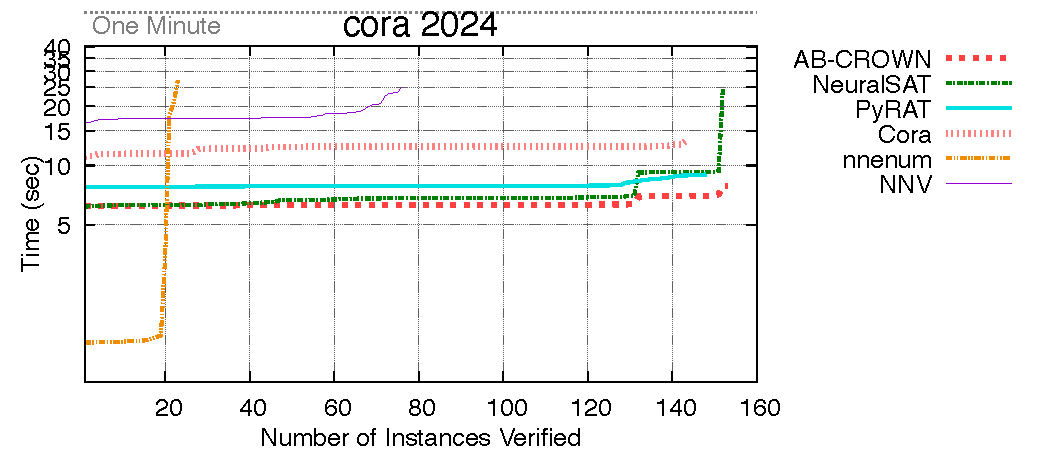
\includegraphics[width=\textwidth]{cactus/2025_cora_2024.pdf}}
\caption{Cactus Plot for cora 2024.}
\label{fig:quantPic}
\end{figure}


\clearpage
% Category 2025_dist_shift_2023 (single_overhead=True):

\begin{table}[h]
\begin{center}
\caption{Benchmark \texttt{2025-dist-shift-2023}} \label{tab:cat_2025_dist_shift_2023}
{\setlength{\tabcolsep}{2pt}
\begin{tabular}[h]{@{}llllllrrr@{}}
\toprule
\textbf{\# ~} & \textbf{Tool} & \textbf{Verified} & \textbf{Falsified} & \textbf{Fastest} & \textbf{Penalty} & \textbf{Points} & \textbf{Score} & \textbf{Solved}\\
\midrule
1 & NeuralSAT & 65 & 7 & 0 & 0 & 720 & 100.0 & 100.0\% \\
2 & CORA & 65 & 7 & 0 & 0 & 720 & 100.0 & 100.0\% \\
3 & $\alpha$-$\beta$-CROWN & 65 & 7 & 0 & 0 & 720 & 100.0 & 100.0\% \\
4 & PyRAT & 64 & 7 & 0 & 0 & 710 & 98.6 & 98.6\% \\
5 & NNV & 50 & 4 & 0 & 0 & 540 & 75.0 & 75.0\% \\
\bottomrule
\end{tabular}
}
\end{center}
\end{table}



\begin{figure}[h]
\centerline{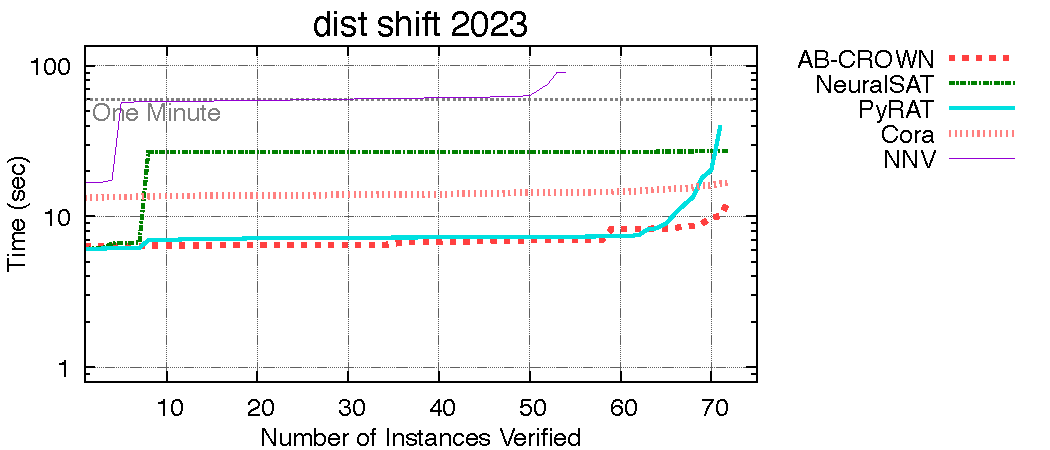
\includegraphics[width=\textwidth]{cactus/2025_dist_shift_2023.pdf}}
\caption{Cactus Plot for dist shift 2023.}
\label{fig:quantPic}
\end{figure}


\clearpage
% Category 2025_linearizenn_2024 (single_overhead=True):

\begin{table}[h]
\begin{center}
\caption{Benchmark \texttt{2025-linearizenn-2024}} \label{tab:cat_2025_linearizenn_2024}
{\setlength{\tabcolsep}{2pt}
\begin{tabular}[h]{@{}llllllrrr@{}}
\toprule
\textbf{\# ~} & \textbf{Tool} & \textbf{Verified} & \textbf{Falsified} & \textbf{Fastest} & \textbf{Penalty} & \textbf{Points} & \textbf{Score} & \textbf{Solved}\\
\midrule
1 & nnenum & 59 & 1 & 0 & 0 & 600 & 100.0 & 100.0\% \\
2 & SobolBox & 59 & 1 & 0 & 0 & 600 & 100.0 & 100.0\% \\
3 & PyRAT & 59 & 1 & 0 & 0 & 600 & 100.0 & 100.0\% \\
4 & NeuralSAT & 59 & 1 & 0 & 0 & 600 & 100.0 & 100.0\% \\
5 & CORA & 59 & 1 & 0 & 0 & 600 & 100.0 & 100.0\% \\
6 & $\alpha$-$\beta$-CROWN & 59 & 1 & 0 & 0 & 600 & 100.0 & 100.0\% \\
7 & NNV & 40 & 1 & 0 & 0 & 410 & 68.3 & 68.3\% \\
\bottomrule
\end{tabular}
}
\end{center}
\end{table}



\begin{figure}[h]
\centerline{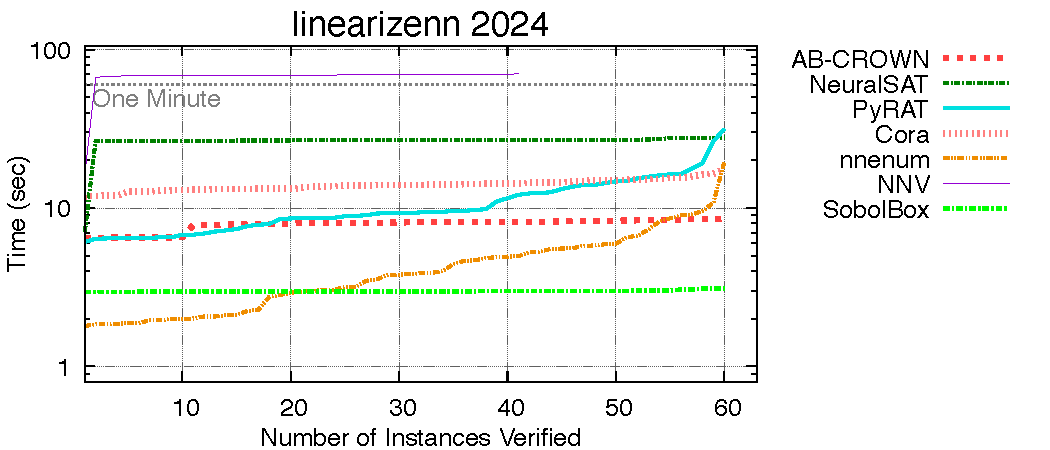
\includegraphics[width=\textwidth]{cactus/2025_linearizenn_2024.pdf}}
\caption{Cactus Plot for linearizenn 2024.}
\label{fig:quantPic}
\end{figure}


\clearpage
% Category 2025_malbeware (single_overhead=True):

\begin{table}[h]
\begin{center}
\caption{Benchmark \texttt{2025-malbeware}} \label{tab:cat_2025_malbeware}
{\setlength{\tabcolsep}{2pt}
\begin{tabular}[h]{@{}llllllrrr@{}}
\toprule
\textbf{\# ~} & \textbf{Tool} & \textbf{Verified} & \textbf{Falsified} & \textbf{Fastest} & \textbf{Penalty} & \textbf{Points} & \textbf{Score} & \textbf{Solved}\\
\midrule
1 & $\alpha$-$\beta$-CROWN & 131 & 19 & 0 & 0 & 1500 & 100.0 & 100.0\% \\
2 & NeuralSAT & 127 & 19 & 0 & 0 & 1460 & 97.3 & 97.3\% \\
3 & PyRAT & 121 & 18 & 0 & 0 & 1390 & 92.7 & 92.7\% \\
4 & nnenum & 125 & 12 & 0 & 0 & 1370 & 91.3 & 91.3\% \\
5 & CORA & 88 & 9 & 0 & 0 & 970 & 64.7 & 64.7\% \\
6 & NNV & 49 & 4 & 0 & 0 & 530 & 35.3 & 35.3\% \\
\bottomrule
\end{tabular}
}
\end{center}
\end{table}



\begin{figure}[h]
\centerline{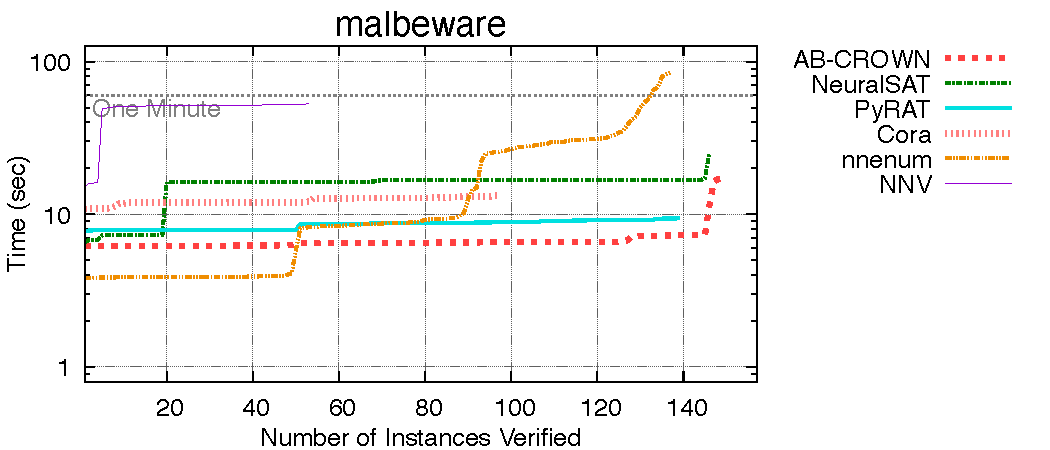
\includegraphics[width=\textwidth]{cactus/2025_malbeware.pdf}}
\caption{Cactus Plot for malbeware.}
\label{fig:quantPic}
\end{figure}


\clearpage
% Category 2025_metaroom_2023 (single_overhead=True):

\begin{table}[h]
\begin{center}
\caption{Benchmark \texttt{2025-metaroom-2023}} \label{tab:cat_2025_metaroom_2023}
{\setlength{\tabcolsep}{2pt}
\begin{tabular}[h]{@{}llllllrrr@{}}
\toprule
\textbf{\# ~} & \textbf{Tool} & \textbf{Verified} & \textbf{Falsified} & \textbf{Fastest} & \textbf{Penalty} & \textbf{Points} & \textbf{Score} & \textbf{Solved}\\
\midrule
1 & NeuralSAT & 94 & 5 & 0 & 0 & 990 & 100.0 & 99.0\% \\
2 & $\alpha$-$\beta$-CROWN & 94 & 5 & 0 & 0 & 990 & 100.0 & 99.0\% \\
3 & CORA & 92 & 5 & 0 & 0 & 970 & 98.0 & 97.0\% \\
4 & NNV & 93 & 2 & 0 & 0 & 950 & 96.0 & 95.0\% \\
5 & PyRAT & 95 & 3 & 0 & 2 & 680 & 68.7 & 98.0\% \\
6 & nnenum & 50 & 1 & 0 & 0 & 510 & 51.5 & 51.0\% \\
\bottomrule
\end{tabular}
}
\end{center}
\end{table}



\begin{figure}[h]
\centerline{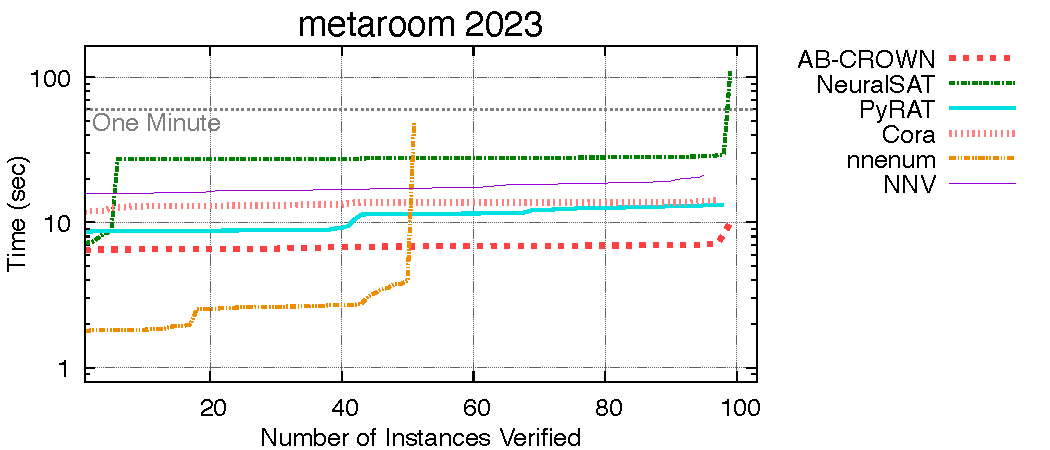
\includegraphics[width=\textwidth]{cactus/2025_metaroom_2023.pdf}}
\caption{Cactus Plot for metaroom 2023.}
\label{fig:quantPic}
\end{figure}


\clearpage
% Category 2025_nn4sys (single_overhead=True):

\begin{table}[h]
\begin{center}
\caption{Benchmark \texttt{2025-nn4sys}} \label{tab:cat_2025_nn4sys}
{\setlength{\tabcolsep}{2pt}
\begin{tabular}[h]{@{}llllllrrr@{}}
\toprule
\textbf{\# ~} & \textbf{Tool} & \textbf{Verified} & \textbf{Falsified} & \textbf{Fastest} & \textbf{Penalty} & \textbf{Points} & \textbf{Score} & \textbf{Solved}\\
\midrule
1 & $\alpha$-$\beta$-CROWN & 194 & 0 & 0 & 0 & 1940 & 100.0 & 100.0\% \\
2 & NeuralSAT & 120 & 0 & 0 & 0 & 1200 & 61.9 & 61.9\% \\
3 & SobolBox & 107 & 0 & 0 & 0 & 1070 & 55.2 & 55.2\% \\
4 & PyRAT & 40 & 0 & 0 & 0 & 400 & 20.6 & 20.6\% \\
5 & nnenum & 22 & 0 & 0 & 0 & 220 & 11.3 & 11.3\% \\
6 & NNV & 17 & 0 & 0 & 0 & 170 & 8.8 & 8.8\% \\
\bottomrule
\end{tabular}
}
\end{center}
\end{table}



\begin{figure}[h]
\centerline{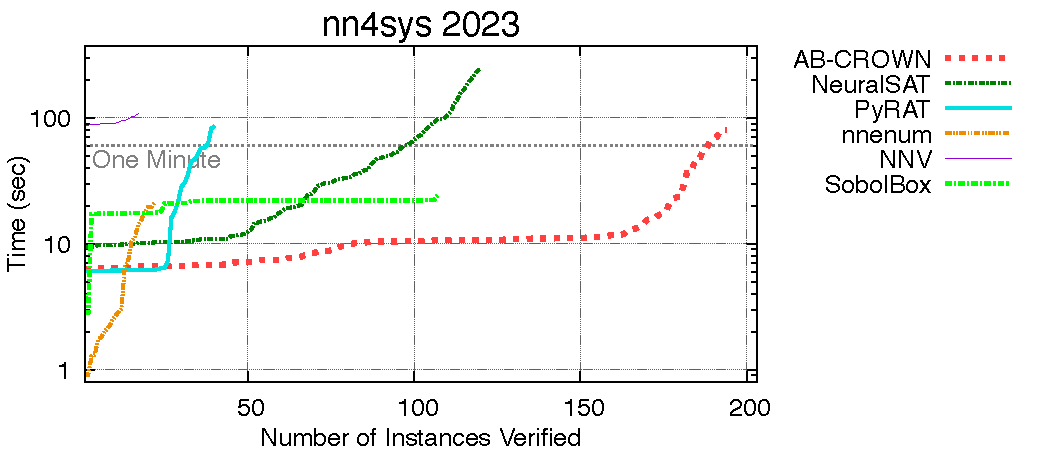
\includegraphics[width=\textwidth]{cactus/2025_nn4sys.pdf}}
\caption{Cactus Plot for nn4sys 2023.}
\label{fig:quantPic}
\end{figure}


\clearpage
% Category 2025_safenlp_2024 (single_overhead=True):

\begin{table}[h]
\begin{center}
\caption{Benchmark \texttt{2025-safenlp-2024}} \label{tab:cat_2025_safenlp_2024}
{\setlength{\tabcolsep}{2pt}
\begin{tabular}[h]{@{}llllllrrr@{}}
\toprule
\textbf{\# ~} & \textbf{Tool} & \textbf{Verified} & \textbf{Falsified} & \textbf{Fastest} & \textbf{Penalty} & \textbf{Points} & \textbf{Score} & \textbf{Solved}\\
\midrule
1 & $\alpha$-$\beta$-CROWN & 433 & 647 & 0 & 0 & 10800 & 100.0 & 100.0\% \\
2 & NeuralSAT & 425 & 645 & 0 & 0 & 10700 & 99.1 & 99.1\% \\
3 & PyRAT & 331 & 647 & 0 & 0 & 9780 & 90.6 & 90.6\% \\
4 & nnenum & 340 & 636 & 0 & 0 & 9760 & 90.4 & 90.4\% \\
5 & CORA & 338 & 644 & 0 & 1 & 9670 & 89.5 & 90.9\% \\
6 & NNV & 172 & 176 & 0 & 0 & 3480 & 32.2 & 32.2\% \\
7 & SobolBox & 413 & 215 & 0 & 403 & -54170 & 0 & 58.1\% \\
\bottomrule
\end{tabular}
}
\end{center}
\end{table}



\begin{figure}[h]
\centerline{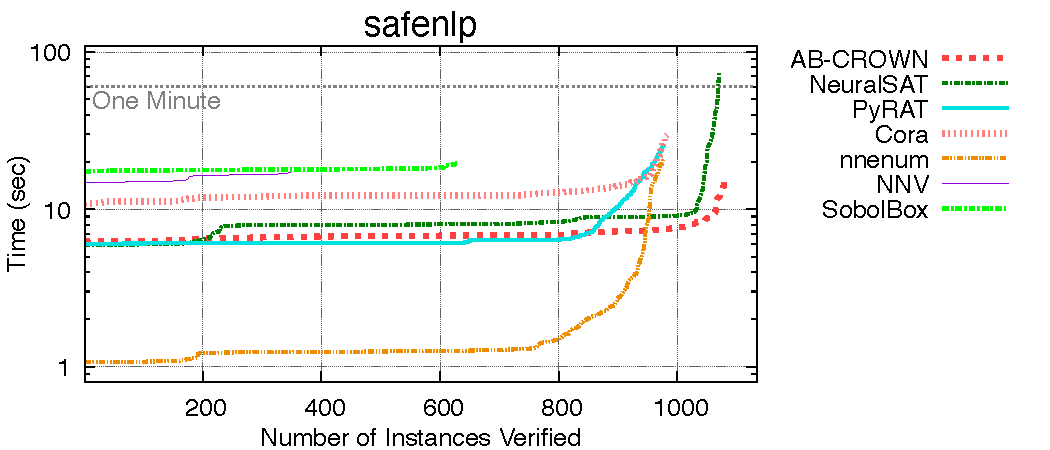
\includegraphics[width=\textwidth]{cactus/2025_safenlp_2024.pdf}}
\caption{Cactus Plot for safenlp.}
\label{fig:quantPic}
\end{figure}


\clearpage
% Category 2025_sat_relu (single_overhead=True):

\begin{table}[h]
\begin{center}
\caption{Benchmark \texttt{2025-sat-relu}} \label{tab:cat_2025_sat_relu}
{\setlength{\tabcolsep}{2pt}
\begin{tabular}[h]{@{}llllllrrr@{}}
\toprule
\textbf{\# ~} & \textbf{Tool} & \textbf{Verified} & \textbf{Falsified} & \textbf{Fastest} & \textbf{Penalty} & \textbf{Points} & \textbf{Score} & \textbf{Solved}\\
\midrule
1 & NeuralSAT & 50 & 50 & 0 & 0 & 1000 & 100.0 & 100.0\% \\
2 & CORA & 50 & 50 & 0 & 0 & 1000 & 100.0 & 100.0\% \\
3 & $\alpha$-$\beta$-CROWN & 50 & 50 & 0 & 0 & 1000 & 100.0 & 100.0\% \\
4 & PyRAT & 9 & 50 & 0 & 0 & 590 & 59.0 & 59.0\% \\
5 & nnenum & 9 & 35 & 0 & 0 & 440 & 44.0 & 44.0\% \\
6 & NNV & 2 & 16 & 0 & 0 & 180 & 18.0 & 18.0\% \\
7 & SobolBox & 0 & 10 & 0 & 33 & -4850 & 0 & 10.0\% \\
\bottomrule
\end{tabular}
}
\end{center}
\end{table}



\begin{figure}[h]
\centerline{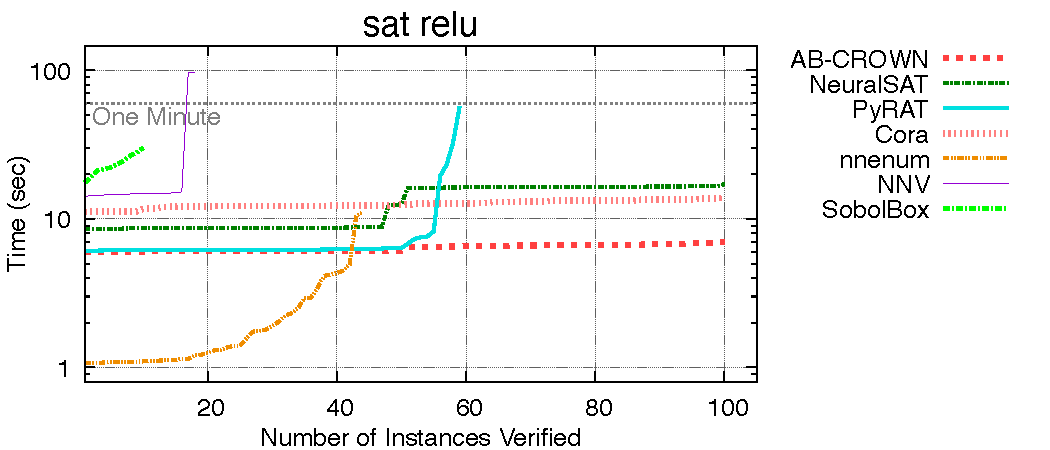
\includegraphics[width=\textwidth]{cactus/2025_sat_relu.pdf}}
\caption{Cactus Plot for sat relu.}
\label{fig:quantPic}
\end{figure}


\clearpage
% Category 2025_soundnessbench (single_overhead=True):

\begin{table}[h]
\begin{center}
\caption{Benchmark \texttt{2025-soundnessbench}} \label{tab:cat_2025_soundnessbench}
{\setlength{\tabcolsep}{2pt}
\begin{tabular}[h]{@{}llllllrrr@{}}
\toprule
\textbf{\# ~} & \textbf{Tool} & \textbf{Verified} & \textbf{Falsified} & \textbf{Fastest} & \textbf{Penalty} & \textbf{Points} & \textbf{Score} & \textbf{Solved}\\
\midrule
1 & $\alpha$-$\beta$-CROWN & 0 & 50 & 0 & 0 & 500 & 100.0 & 100.0\% \\
2 & NeuralSAT & 0 & 30 & 0 & 12 & -1500 & 0 & 60.0\% \\
3 & CORA & 0 & 0 & 0 & 18 & -2700 & 0 & 0.0\% \\
\bottomrule
\end{tabular}
}
\end{center}
\end{table}



\begin{figure}[h]
\centerline{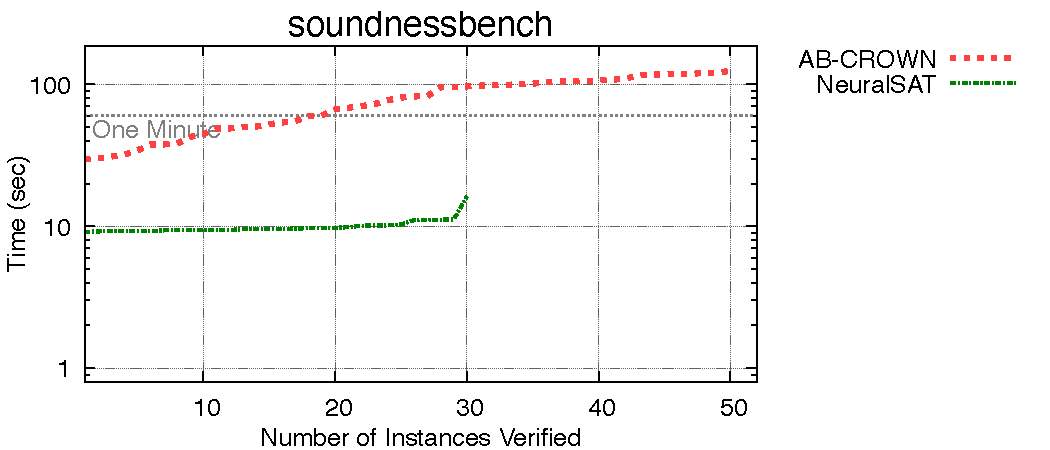
\includegraphics[width=\textwidth]{cactus/2025_soundnessbench.pdf}}
\caption{Cactus Plot for soundnessbench.}
\label{fig:quantPic}
\end{figure}


\clearpage
% Category 2025_tinyimagenet_2024 (single_overhead=True):

\begin{table}[h]
\begin{center}
\caption{Benchmark \texttt{2025-tinyimagenet-2024}} \label{tab:cat_2025_tinyimagenet_2024}
{\setlength{\tabcolsep}{2pt}
\begin{tabular}[h]{@{}llllllrrr@{}}
\toprule
\textbf{\# ~} & \textbf{Tool} & \textbf{Verified} & \textbf{Falsified} & \textbf{Fastest} & \textbf{Penalty} & \textbf{Points} & \textbf{Score} & \textbf{Solved}\\
\midrule
1 & $\alpha$-$\beta$-CROWN & 137 & 38 & 0 & 0 & 1750 & 100.0 & 87.5\% \\
2 & NeuralSAT & 116 & 37 & 0 & 1 & 1380 & 78.9 & 76.5\% \\
3 & PyRAT & 68 & 35 & 0 & 0 & 1030 & 58.9 & 51.5\% \\
4 & CORA & 0 & 5 & 0 & 0 & 50 & 2.9 & 2.5\% \\
5 & NNV & 0 & 1 & 0 & 0 & 10 & 0.6 & 0.5\% \\
\bottomrule
\end{tabular}
}
\end{center}
\end{table}



\begin{figure}[h]
\centerline{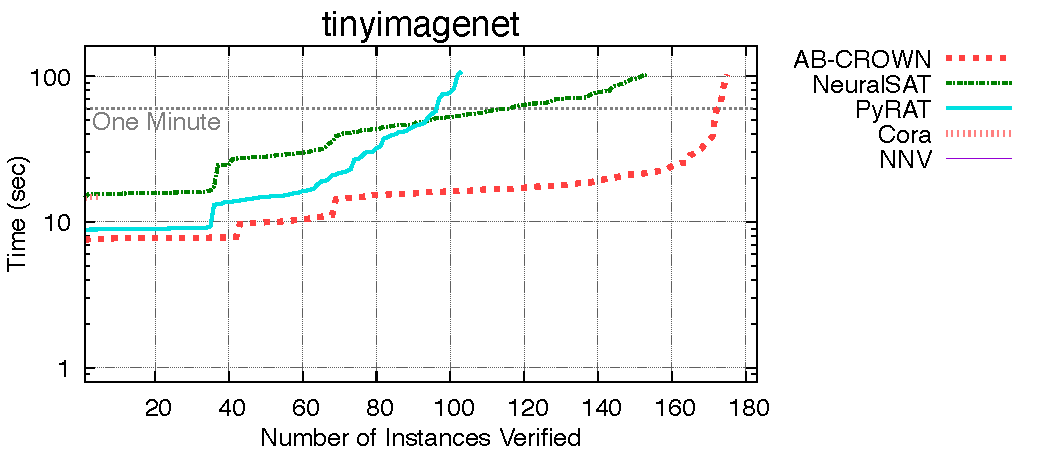
\includegraphics[width=\textwidth]{cactus/2025_tinyimagenet_2024.pdf}}
\caption{Cactus Plot for tinyimagenet.}
\label{fig:quantPic}
\end{figure}


\clearpage
% Category 2025_tllverifybench_2023 (single_overhead=True):

\begin{table}[h]
\begin{center}
\caption{Benchmark \texttt{2025-tllverifybench-2023}} \label{tab:cat_2025_tllverifybench_2023}
{\setlength{\tabcolsep}{2pt}
\begin{tabular}[h]{@{}llllllrrr@{}}
\toprule
\textbf{\# ~} & \textbf{Tool} & \textbf{Verified} & \textbf{Falsified} & \textbf{Fastest} & \textbf{Penalty} & \textbf{Points} & \textbf{Score} & \textbf{Solved}\\
\midrule
1 & SobolBox & 15 & 17 & 0 & 0 & 320 & 100.0 & 100.0\% \\
2 & PyRAT & 15 & 17 & 0 & 0 & 320 & 100.0 & 100.0\% \\
3 & NeuralSAT & 15 & 17 & 0 & 0 & 320 & 100.0 & 100.0\% \\
4 & CORA & 15 & 17 & 0 & 0 & 320 & 100.0 & 100.0\% \\
5 & $\alpha$-$\beta$-CROWN & 15 & 17 & 0 & 0 & 320 & 100.0 & 100.0\% \\
6 & nnenum & 1 & 17 & 0 & 0 & 180 & 56.2 & 56.2\% \\
7 & NNV & 0 & 17 & 0 & 0 & 170 & 53.1 & 53.1\% \\
\bottomrule
\end{tabular}
}
\end{center}
\end{table}



\begin{figure}[h]
\centerline{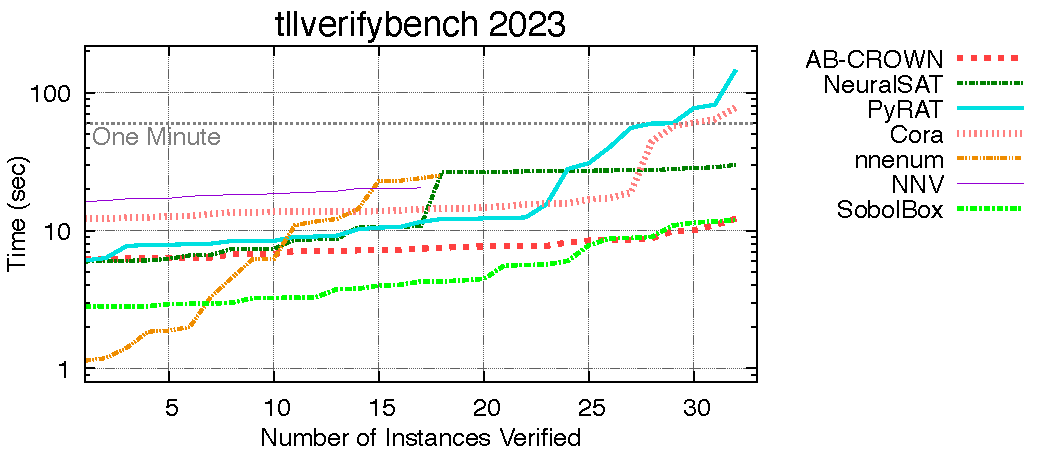
\includegraphics[width=\textwidth]{cactus/2025_tllverifybench_2023.pdf}}
\caption{Cactus Plot for tllverifybench 2023.}
\label{fig:quantPic}
\end{figure}



\clearpage
\section{Unscored Benchmarks}

\clearpage
% Category 2024_acasxu_2023 (single_overhead=True):

\begin{table}[h]
\begin{center}
\caption{Benchmark \texttt{2024-acasxu-2023}} \label{tab:cat_{cat}}
{\setlength{\tabcolsep}{2pt}
\begin{tabular}[h]{@{}llllllrrr@{}}
\toprule
\textbf{\# ~} & \textbf{Tool} & \textbf{Verified} & \textbf{Falsified} & \textbf{Fastest} & \textbf{Penalty} & \textbf{Points} & \textbf{Score} & \textbf{Solved}\\
\midrule
1 & $\alpha$-$\beta$-CROWN & 139 & 47 & 0 & 0 & 1860 & 100.0 & 100.0\% \\
2 & nnenum & 139 & 46 & 0 & 0 & 1850 & 99.5 & 99.5\% \\
3 & PyRAT & 137 & 47 & 0 & 0 & 1840 & 98.9 & 98.9\% \\
4 & Marabou & 134 & 45 & 0 & 1 & 1640 & 88.2 & 96.2\% \\
5 & NeVer2 & 121 & 40 & 0 & 0 & 1610 & 86.6 & 86.6\% \\
6 & NNV & 70 & 27 & 0 & 0 & 970 & 52.2 & 52.2\% \\
7 & CORA & 134 & 7 & 0 & 36 & -3990 & 0 & 75.8\% \\
8 & NeuralSAT & 138 & 0 & 0 & 46 & -5520 & 0 & 74.2\% \\
\bottomrule
\end{tabular}
}
\end{center}
\end{table}



\begin{figure}[h]
\centerline{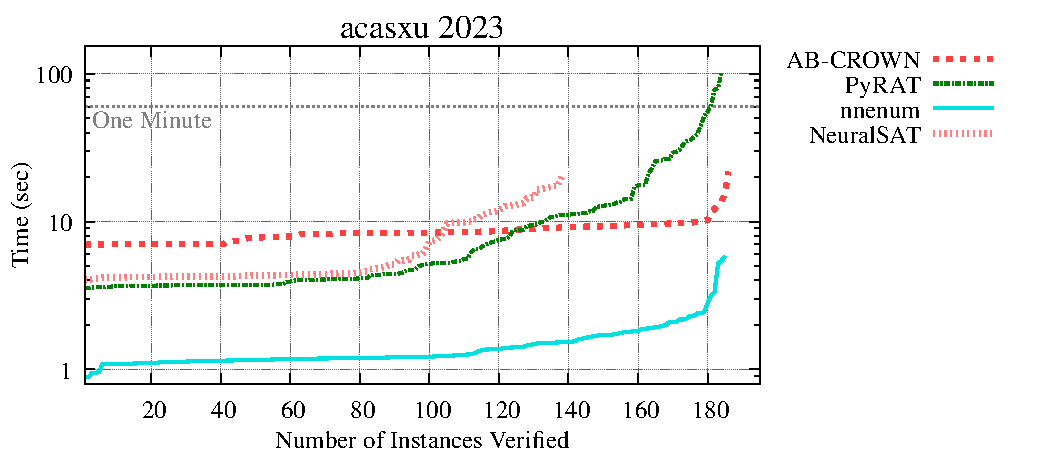
\includegraphics[width=\textwidth]{cactus/2024_acasxu_2023.pdf}}
\caption{Cactus Plot for acasxu 2023.}
\label{fig:quantPic}
\end{figure}


\clearpage
% Category 2024_cgan_2023 (single_overhead=True):

\begin{table}[h]
\begin{center}
\caption{Benchmark \texttt{2024-cgan-2023}} \label{tab:cat_{cat}}
{\setlength{\tabcolsep}{2pt}
\begin{tabular}[h]{@{}llllllrrr@{}}
\toprule
\textbf{\# ~} & \textbf{Tool} & \textbf{Verified} & \textbf{Falsified} & \textbf{Fastest} & \textbf{Penalty} & \textbf{Points} & \textbf{Score} & \textbf{Solved}\\
\midrule
1 & PyRAT & 8 & 13 & 0 & 0 & 210 & 100.0 & 100.0\% \\
2 & $\alpha$-$\beta$-CROWN & 8 & 13 & 0 & 0 & 210 & 100.0 & 100.0\% \\
3 & nnenum & 6 & 11 & 0 & 0 & 170 & 81.0 & 81.0\% \\
4 & NNV & 6 & 11 & 0 & 0 & 170 & 81.0 & 81.0\% \\
5 & Marabou & 0 & 13 & 0 & 0 & 130 & 61.9 & 61.9\% \\
6 & NeuralSAT & 8 & 0 & 0 & 11 & -1570 & 0 & 38.1\% \\
\bottomrule
\end{tabular}
}
\end{center}
\end{table}



\begin{figure}[h]
\centerline{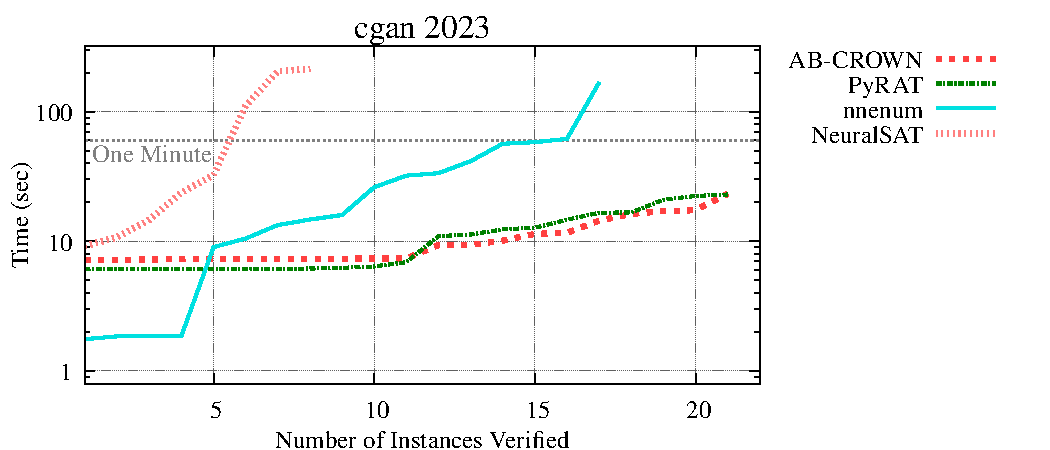
\includegraphics[width=\textwidth]{cactus/2024_cgan_2023.pdf}}
\caption{Cactus Plot for cgan 2023.}
\label{fig:quantPic}
\end{figure}


\clearpage
% Category 2024_cifar100 (single_overhead=True):

\begin{table}[h]
\begin{center}
\caption{Benchmark \texttt{2024-cifar100}} \label{tab:cat_{cat}}
{\setlength{\tabcolsep}{2pt}
\begin{tabular}[h]{@{}llllllrrr@{}}
\toprule
\textbf{\# ~} & \textbf{Tool} & \textbf{Verified} & \textbf{Falsified} & \textbf{Fastest} & \textbf{Penalty} & \textbf{Points} & \textbf{Score} & \textbf{Solved}\\
\midrule
1 & $\alpha$-$\beta$-CROWN & 117 & 32 & 0 & 0 & 1490 & 100.0 & 74.5\% \\
2 & PyRAT & 67 & 25 & 0 & 0 & 920 & 61.7 & 46.0\% \\
3 & Marabou & 0 & 30 & 0 & 0 & 300 & 20.1 & 15.0\% \\
4 & NeuralSAT & 89 & 0 & 0 & 23 & -2560 & 0 & 44.5\% \\
\bottomrule
\end{tabular}
}
\end{center}
\end{table}



\begin{figure}[h]
\centerline{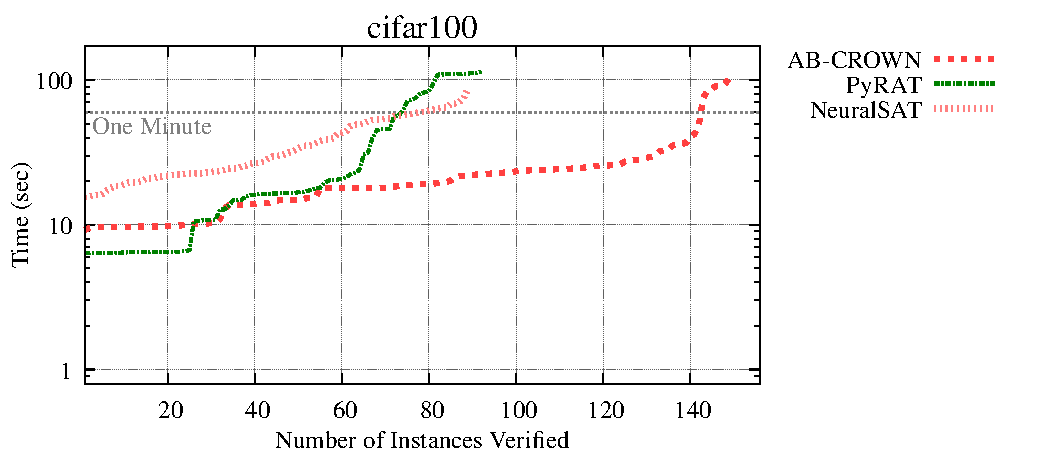
\includegraphics[width=\textwidth]{cactus/2024_cifar100.pdf}}
\caption{Cactus Plot for cifar100.}
\label{fig:quantPic}
\end{figure}


\clearpage
% Category 2024_collins_rul_cnn_2023 (single_overhead=True):

\begin{table}[h]
\begin{center}
\caption{Benchmark \texttt{2024-collins-rul-cnn-2023}} \label{tab:cat_{cat}}
{\setlength{\tabcolsep}{2pt}
\begin{tabular}[h]{@{}llllllrrr@{}}
\toprule
\textbf{\# ~} & \textbf{Tool} & \textbf{Verified} & \textbf{Falsified} & \textbf{Fastest} & \textbf{Penalty} & \textbf{Points} & \textbf{Score} & \textbf{Solved}\\
\midrule
1 & nnenum & 30 & 32 & 0 & 0 & 620 & 100.0 & 100.0\% \\
2 & NNV & 30 & 32 & 0 & 0 & 620 & 100.0 & 100.0\% \\
3 & Marabou & 30 & 32 & 0 & 0 & 620 & 100.0 & 100.0\% \\
4 & $\alpha$-$\beta$-CROWN & 30 & 32 & 0 & 0 & 620 & 100.0 & 100.0\% \\
5 & PyRAT & 30 & 28 & 0 & 0 & 580 & 93.5 & 93.5\% \\
6 & CORA & 0 & 19 & 0 & 11 & -1460 & 0 & 30.6\% \\
7 & NeuralSAT & 30 & 0 & 0 & 32 & -4500 & 0 & 48.4\% \\
\bottomrule
\end{tabular}
}
\end{center}
\end{table}



\begin{figure}[h]
\centerline{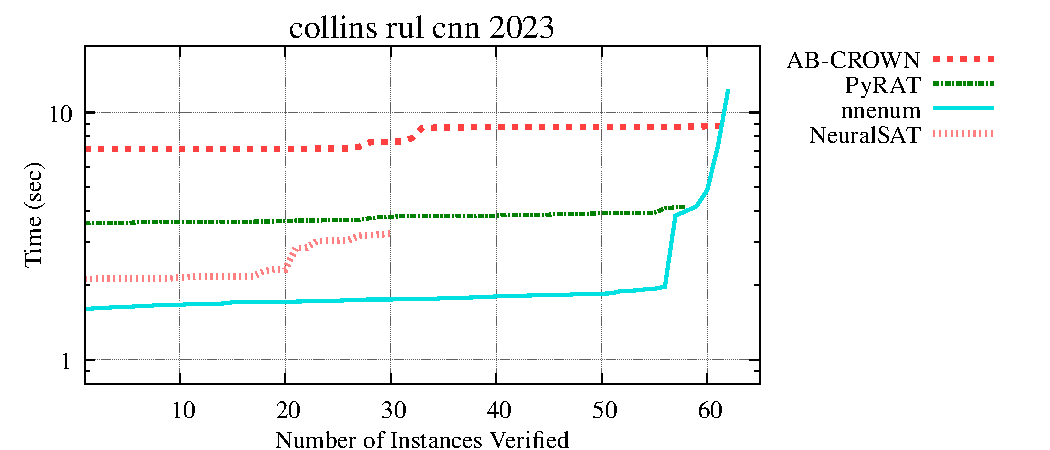
\includegraphics[width=\textwidth]{cactus/2024_collins_rul_cnn_2023.pdf}}
\caption{Cactus Plot for collins rul cnn 2023.}
\label{fig:quantPic}
\end{figure}


\clearpage
% Category 2024_cora (single_overhead=True):

\begin{table}[h]
\begin{center}
\caption{Benchmark \texttt{2024-cora}} \label{tab:cat_{cat}}
{\setlength{\tabcolsep}{2pt}
\begin{tabular}[h]{@{}llllllrrr@{}}
\toprule
\textbf{\# ~} & \textbf{Tool} & \textbf{Verified} & \textbf{Falsified} & \textbf{Fastest} & \textbf{Penalty} & \textbf{Points} & \textbf{Score} & \textbf{Solved}\\
\midrule
1 & $\alpha$-$\beta$-CROWN & 24 & 134 & 0 & 0 & 1580 & 100.0 & 87.8\% \\
2 & Marabou & 22 & 134 & 0 & 0 & 1560 & 98.7 & 86.7\% \\
3 & PyRAT & 22 & 128 & 0 & 0 & 1500 & 94.9 & 83.3\% \\
4 & NNV & 15 & 47 & 0 & 0 & 620 & 39.2 & 34.4\% \\
5 & NeVer2 & 17 & 11 & 0 & 0 & 280 & 17.7 & 15.6\% \\
6 & nnenum & 20 & 6 & 0 & 0 & 260 & 16.5 & 14.4\% \\
7 & CORA & 21 & 5 & 0 & 54 & -7840 & 0 & 14.4\% \\
8 & NeuralSAT & 23 & 0 & 0 & 134 & -19870 & 0 & 12.8\% \\
\bottomrule
\end{tabular}
}
\end{center}
\end{table}



\begin{figure}[h]
\centerline{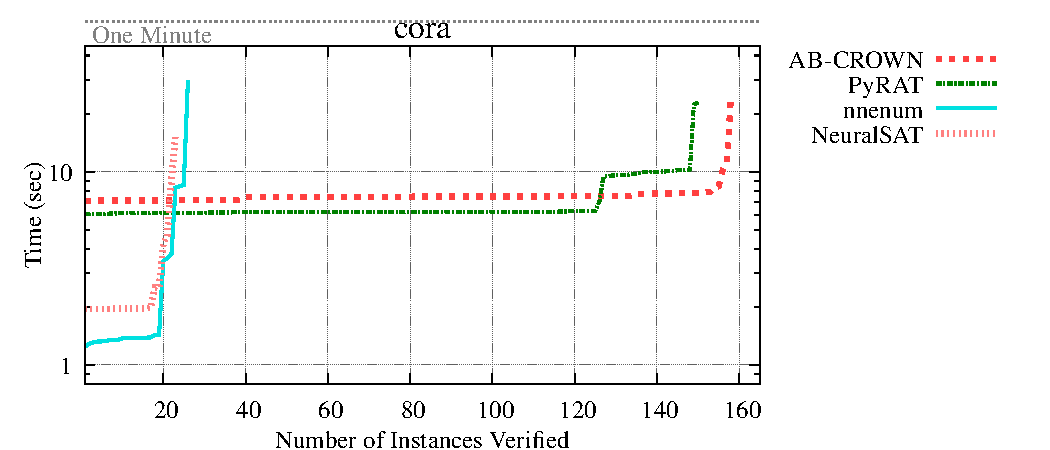
\includegraphics[width=\textwidth]{cactus/2024_cora.pdf}}
\caption{Cactus Plot for cora.}
\label{fig:quantPic}
\end{figure}


\clearpage
% Category 2024_dist_shift_2023 (single_overhead=True):

\begin{table}[h]
\begin{center}
\caption{Benchmark \texttt{2024-dist-shift-2023}} \label{tab:cat_{cat}}
{\setlength{\tabcolsep}{2pt}
\begin{tabular}[h]{@{}llllllrrr@{}}
\toprule
\textbf{\# ~} & \textbf{Tool} & \textbf{Verified} & \textbf{Falsified} & \textbf{Fastest} & \textbf{Penalty} & \textbf{Points} & \textbf{Score} & \textbf{Solved}\\
\midrule
1 & PyRAT & 63 & 8 & 0 & 0 & 710 & 100.0 & 98.6\% \\
2 & CORA & 63 & 8 & 0 & 0 & 710 & 100.0 & 98.6\% \\
3 & $\alpha$-$\beta$-CROWN & 63 & 8 & 0 & 0 & 710 & 100.0 & 98.6\% \\
4 & Marabou & 62 & 7 & 0 & 0 & 690 & 97.2 & 95.8\% \\
5 & NNV & 51 & 5 & 0 & 0 & 560 & 78.9 & 77.8\% \\
\bottomrule
\end{tabular}
}
\end{center}
\end{table}



\begin{figure}[h]
\centerline{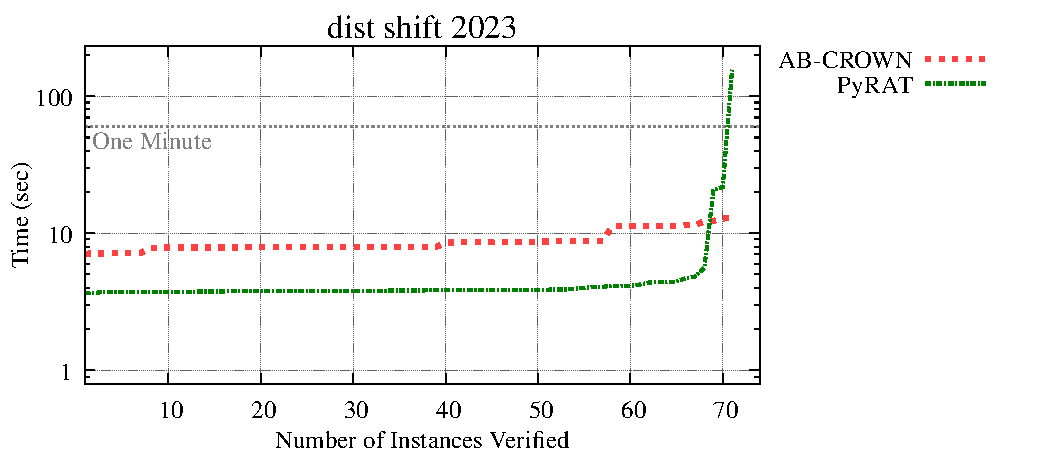
\includegraphics[width=\textwidth]{cactus/2024_dist_shift_2023.pdf}}
\caption{Cactus Plot for dist shift 2023.}
\label{fig:quantPic}
\end{figure}


\clearpage
% Category 2024_linearizenn (single_overhead=True):

\begin{table}[h]
\begin{center}
\caption{Benchmark \texttt{2024-linearizenn}} \label{tab:cat_{cat}}
{\setlength{\tabcolsep}{2pt}
\begin{tabular}[h]{@{}llllllrrr@{}}
\toprule
\textbf{\# ~} & \textbf{Tool} & \textbf{Verified} & \textbf{Falsified} & \textbf{Fastest} & \textbf{Penalty} & \textbf{Points} & \textbf{Score} & \textbf{Solved}\\
\midrule
1 & PyRAT & 59 & 1 & 0 & 0 & 600 & 100.0 & 100.0\% \\
2 & Marabou & 59 & 1 & 0 & 0 & 600 & 100.0 & 100.0\% \\
3 & $\alpha$-$\beta$-CROWN & 59 & 1 & 0 & 0 & 600 & 100.0 & 100.0\% \\
4 & nnenum & 59 & 0 & 0 & 1 & 440 & 73.3 & 98.3\% \\
\bottomrule
\end{tabular}
}
\end{center}
\end{table}



\begin{figure}[h]
\centerline{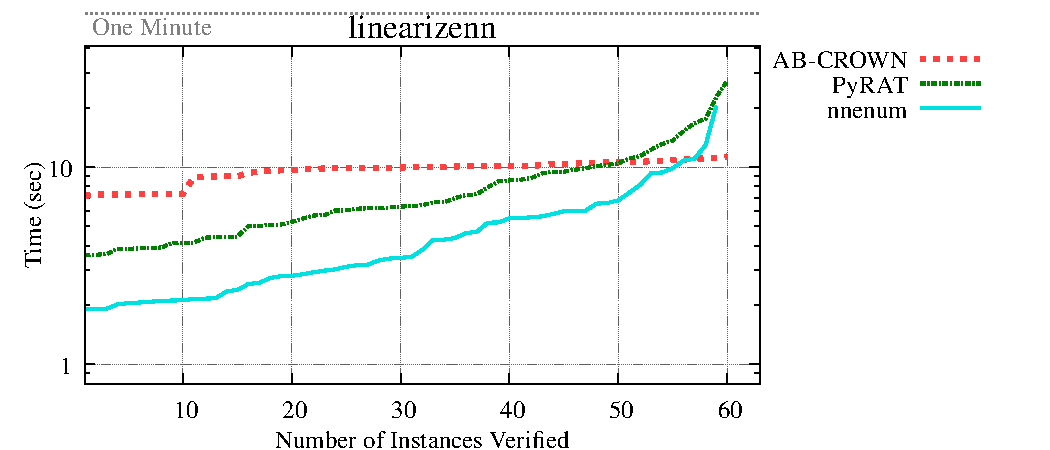
\includegraphics[width=\textwidth]{cactus/2024_linearizenn.pdf}}
\caption{Cactus Plot for linearizenn.}
\label{fig:quantPic}
\end{figure}


\clearpage
% Category 2024_metaroom_2023 (single_overhead=True):

\begin{table}[h]
\begin{center}
\caption{Benchmark \texttt{2024-metaroom-2023}} \label{tab:cat_{cat}}
{\setlength{\tabcolsep}{2pt}
\begin{tabular}[h]{@{}llllllrrr@{}}
\toprule
\textbf{\# ~} & \textbf{Tool} & \textbf{Verified} & \textbf{Falsified} & \textbf{Fastest} & \textbf{Penalty} & \textbf{Points} & \textbf{Score} & \textbf{Solved}\\
\midrule
1 & $\alpha$-$\beta$-CROWN & 91 & 7 & 0 & 0 & 980 & 100.0 & 98.0\% \\
2 & PyRAT & 91 & 6 & 0 & 0 & 970 & 99.0 & 97.0\% \\
3 & NNV & 90 & 2 & 0 & 0 & 920 & 93.9 & 92.0\% \\
4 & Marabou & 46 & 7 & 0 & 0 & 530 & 54.1 & 53.0\% \\
5 & nnenum & 44 & 2 & 0 & 0 & 460 & 46.9 & 46.0\% \\
6 & NeuralSAT & 91 & 0 & 0 & 7 & -140 & 0 & 91.0\% \\
\bottomrule
\end{tabular}
}
\end{center}
\end{table}



\begin{figure}[h]
\centerline{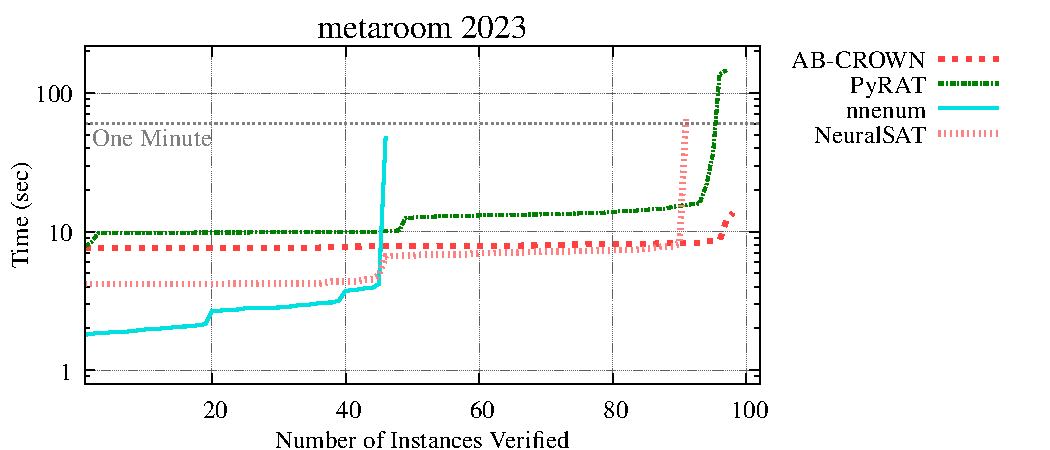
\includegraphics[width=\textwidth]{cactus/2024_metaroom_2023.pdf}}
\caption{Cactus Plot for metaroom 2023.}
\label{fig:quantPic}
\end{figure}


\clearpage
% Category 2024_nn4sys_2023 (single_overhead=True):

\begin{table}[h]
\begin{center}
\caption{Benchmark \texttt{2024-nn4sys-2023}} \label{tab:cat_{cat}}
{\setlength{\tabcolsep}{2pt}
\begin{tabular}[h]{@{}llllllrrr@{}}
\toprule
\textbf{\# ~} & \textbf{Tool} & \textbf{Verified} & \textbf{Falsified} & \textbf{Fastest} & \textbf{Penalty} & \textbf{Points} & \textbf{Score} & \textbf{Solved}\\
\midrule
1 & $\alpha$-$\beta$-CROWN & 194 & 0 & 0 & 0 & 1940 & 100.0 & 100.0\% \\
2 & PyRAT & 53 & 0 & 0 & 0 & 530 & 27.3 & 27.3\% \\
3 & Marabou & 24 & 0 & 0 & 0 & 240 & 12.4 & 12.4\% \\
4 & nnenum & 22 & 0 & 0 & 0 & 220 & 11.3 & 11.3\% \\
5 & CORA & 2 & 0 & 0 & 0 & 20 & 1.0 & 1.0\% \\
\bottomrule
\end{tabular}
}
\end{center}
\end{table}



\begin{figure}[h]
\centerline{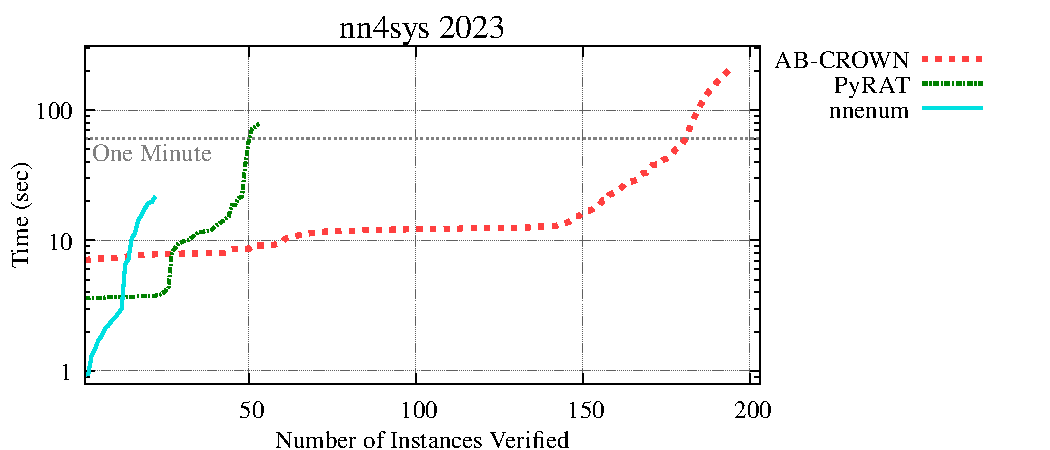
\includegraphics[width=\textwidth]{cactus/2024_nn4sys_2023.pdf}}
\caption{Cactus Plot for nn4sys 2023.}
\label{fig:quantPic}
\end{figure}


\clearpage
% Category 2024_safenlp (single_overhead=True):

\begin{table}[h]
\begin{center}
\caption{Benchmark \texttt{2024-safenlp}} \label{tab:cat_{cat}}
{\setlength{\tabcolsep}{2pt}
\begin{tabular}[h]{@{}llllllrrr@{}}
\toprule
\textbf{\# ~} & \textbf{Tool} & \textbf{Verified} & \textbf{Falsified} & \textbf{Fastest} & \textbf{Penalty} & \textbf{Points} & \textbf{Score} & \textbf{Solved}\\
\midrule
1 & $\alpha$-$\beta$-CROWN & 421 & 659 & 0 & 0 & 10800 & 100.0 & 100.0\% \\
2 & nnenum & 321 & 642 & 0 & 1 & 9480 & 87.8 & 89.2\% \\
3 & PyRAT & 277 & 586 & 0 & 0 & 8630 & 79.9 & 79.9\% \\
4 & NeVer2 & 161 & 466 & 0 & 0 & 6270 & 58.1 & 58.1\% \\
5 & CORA & 266 & 269 & 0 & 0 & 5350 & 49.5 & 49.5\% \\
6 & NNV & 166 & 165 & 0 & 0 & 3310 & 30.6 & 30.6\% \\
7 & Marabou & 300 & 375 & 0 & 402 & -53550 & 0 & 62.5\% \\
\bottomrule
\end{tabular}
}
\end{center}
\end{table}



\begin{figure}[h]
\centerline{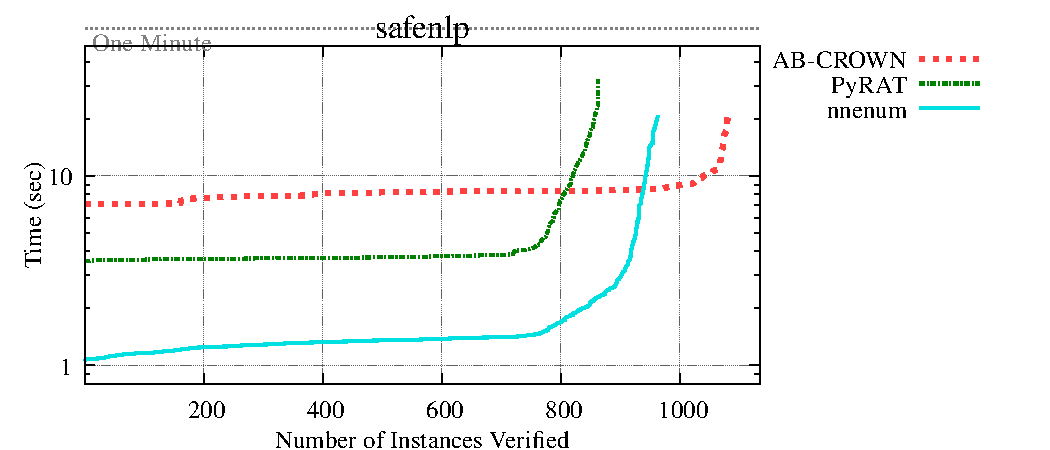
\includegraphics[width=\textwidth]{cactus/2024_safenlp.pdf}}
\caption{Cactus Plot for safenlp.}
\label{fig:quantPic}
\end{figure}


\clearpage
% Category 2024_tinyimagenet (single_overhead=True):

\begin{table}[h]
\begin{center}
\caption{Benchmark \texttt{2024-tinyimagenet}} \label{tab:cat_{cat}}
{\setlength{\tabcolsep}{2pt}
\begin{tabular}[h]{@{}llllllrrr@{}}
\toprule
\textbf{\# ~} & \textbf{Tool} & \textbf{Verified} & \textbf{Falsified} & \textbf{Fastest} & \textbf{Penalty} & \textbf{Points} & \textbf{Score} & \textbf{Solved}\\
\midrule
1 & $\alpha$-$\beta$-CROWN & 131 & 43 & 0 & 0 & 1740 & 100.0 & 87.0\% \\
2 & PyRAT & 48 & 31 & 0 & 0 & 790 & 45.4 & 39.5\% \\
3 & Marabou & 0 & 43 & 0 & 0 & 430 & 24.7 & 21.5\% \\
4 & NNV & 0 & 2 & 0 & 0 & 20 & 1.1 & 1.0\% \\
5 & CORA & 0 & 2 & 0 & 0 & 20 & 1.1 & 1.0\% \\
6 & NeuralSAT & 95 & 0 & 0 & 11 & -700 & 0 & 47.5\% \\
\bottomrule
\end{tabular}
}
\end{center}
\end{table}



\begin{figure}[h]
\centerline{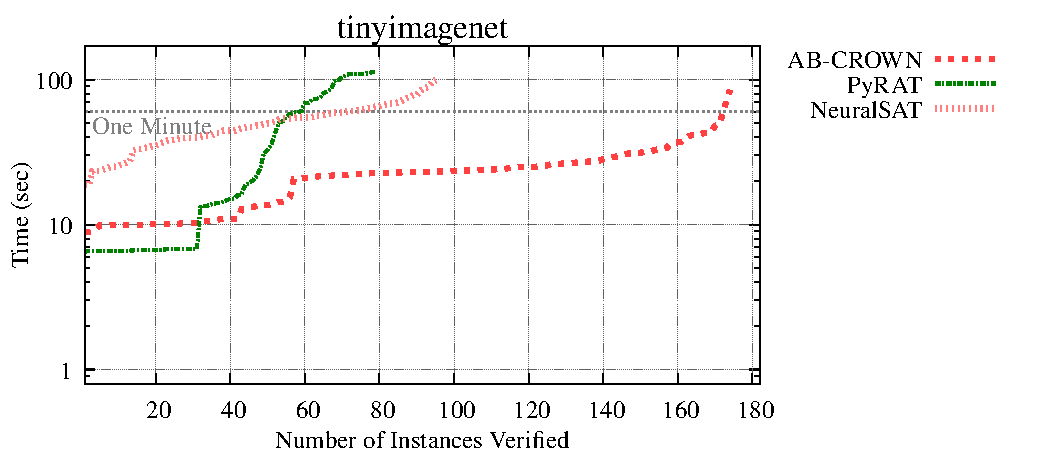
\includegraphics[width=\textwidth]{cactus/2024_tinyimagenet.pdf}}
\caption{Cactus Plot for tinyimagenet.}
\label{fig:quantPic}
\end{figure}


\clearpage
% Category 2024_tllverifybench_2023 (single_overhead=True):

\begin{table}[h]
\begin{center}
\caption{Benchmark \texttt{2024-tllverifybench-2023}} \label{tab:cat_{cat}}
{\setlength{\tabcolsep}{2pt}
\begin{tabular}[h]{@{}llllllrrr@{}}
\toprule
\textbf{\# ~} & \textbf{Tool} & \textbf{Verified} & \textbf{Falsified} & \textbf{Fastest} & \textbf{Penalty} & \textbf{Points} & \textbf{Score} & \textbf{Solved}\\
\midrule
1 & PyRAT & 15 & 17 & 0 & 0 & 320 & 100.0 & 100.0\% \\
2 & NeVer2 & 23 & 9 & 0 & 0 & 320 & 100.0 & 100.0\% \\
3 & CORA & 15 & 17 & 0 & 0 & 320 & 100.0 & 100.0\% \\
4 & $\alpha$-$\beta$-CROWN & 15 & 17 & 0 & 0 & 320 & 100.0 & 100.0\% \\
5 & Marabou & 13 & 17 & 0 & 0 & 300 & 93.8 & 93.8\% \\
6 & nnenum & 2 & 16 & 0 & 0 & 180 & 56.2 & 56.2\% \\
7 & NNV & 0 & 17 & 0 & 0 & 170 & 53.1 & 53.1\% \\
8 & NeuralSAT & 15 & 0 & 0 & 17 & -2400 & 0 & 46.9\% \\
\bottomrule
\end{tabular}
}
\end{center}
\end{table}



\begin{figure}[h]
\centerline{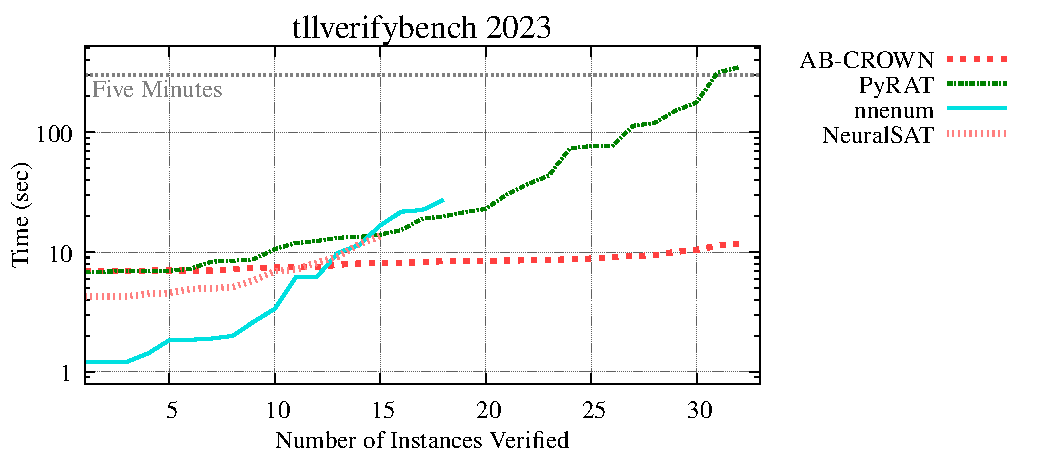
\includegraphics[width=\textwidth]{cactus/2024_tllverifybench_2023.pdf}}
\caption{Cactus Plot for tllverifybench 2023.}
\label{fig:quantPic}
\end{figure}



\clearpage
\section{Stats}

%%%%%%%%%% Stats %%%%%%%%%%%

% Overhead:

\begin{table}[h]
\begin{center}
\caption{Overhead} \label{tab:overhead}
{\setlength{\tabcolsep}{2pt}
\begin{tabular}[h]{@{}llr@{}}
\toprule
\textbf{\# ~} & \textbf{Tool} & \textbf{Seconds}\\
\midrule
1 & NeuralSAT & 1.0 \\
2 & nnenum & 1.3 \\
3 & PyRAT & 3.6 \\
4 & $\alpha$-$\beta$-CROWN & 7.0 \\
5 & CORA & inf \\
6 & Marabou & inf \\
7 & NeVer2 & inf \\
8 & NNV & inf \\
\bottomrule
\end{tabular}
}
\end{center}
\end{table}



% Num Benchmarks Participated:

\begin{table}[h]
\begin{center}
\caption{Num Benchmarks Participated} \label{tab:stats0}
{\setlength{\tabcolsep}{2pt}
\begin{tabular}[h]{@{}llr@{}}
\toprule
\textbf{\# ~} & \textbf{Tool} & \textbf{Count}\\
\midrule
1 & $\alpha$-$\beta$-CROWN & 9 \\
2 & PyRAT & 8 \\
3 & NeuralSAT & 3 \\
4 & nnenum & 1 \\
5 & NeVer2 & 0 \\
6 & NNV & 0 \\
7 & Marabou & 0 \\
8 & CORA & 0 \\
\bottomrule
\end{tabular}
}
\end{center}
\end{table}



% Num Instances Verified:

\begin{table}[h]
\begin{center}
\caption{Num Instances Verified} \label{tab:stats1}
{\setlength{\tabcolsep}{2pt}
\begin{tabular}[h]{@{}llr@{}}
\toprule
\textbf{\# ~} & \textbf{Tool} & \textbf{Count}\\
\midrule
1 & $\alpha$-$\beta$-CROWN & 376 \\
2 & PyRAT & 127 \\
3 & NeuralSAT & 17 \\
4 & nnenum & 13 \\
\bottomrule
\end{tabular}
}
\end{center}
\end{table}



% Num SAT:

\begin{table}[h]
\begin{center}
\caption{Num SAT} \label{tab:stats2}
{\setlength{\tabcolsep}{2pt}
\begin{tabular}[h]{@{}llr@{}}
\toprule
\textbf{\# ~} & \textbf{Tool} & \textbf{Count}\\
\midrule
1 & $\alpha$-$\beta$-CROWN & 82 \\
2 & PyRAT & 15 \\
\bottomrule
\end{tabular}
}
\end{center}
\end{table}



% Num UNSAT:

\begin{table}[h]
\begin{center}
\caption{Num UNSAT} \label{tab:stats3}
{\setlength{\tabcolsep}{2pt}
\begin{tabular}[h]{@{}llr@{}}
\toprule
\textbf{\# ~} & \textbf{Tool} & \textbf{Count}\\
\midrule
1 & $\alpha$-$\beta$-CROWN & 294 \\
2 & PyRAT & 112 \\
3 & NeuralSAT & 17 \\
4 & nnenum & 13 \\
\bottomrule
\end{tabular}
}
\end{center}
\end{table}



% Incorrect Results (or Missing CE):

\begin{table}[h]
\begin{center}
\caption{Incorrect Results (or Missing CE)} \label{tab:stats4}
{\setlength{\tabcolsep}{2pt}
\begin{tabular}[h]{@{}llr@{}}
\toprule
\textbf{\# ~} & \textbf{Tool} & \textbf{Count}\\
\midrule
1 & NeuralSAT & 11 \\
\bottomrule
\end{tabular}
}
\end{center}
\end{table}




\clearpage
\section{Detailed Results}
% Long table of all results


\begin{center}
{\setlength{\tabcolsep}{1pt}
\scriptsize
\begin{longtable}{@{}llllllllll@{}}
\caption{\footnotesize Instance Runtimes. Fastest times are \textcolor{blue}{blue}. Second fastest are \textcolor{second}{green}. Penalties are red crosses (\textbf{\textcolor{red}{\ding{55}}}).} \label{tab:all_results} \\
\toprule
\textbf{Category} & \textbf{Id} & \textbf{Result} & \textbf{$\alpha$-$\beta$-C} & \textbf{NSAT} & \textbf{PyRAT} & \textbf{CORA} & \textbf{NNen} & \textbf{NNV} & \textbf{SB} \\
\midrule
\endhead
2025 Acasxu 2023 & 0 & ~\textsc{unsat} & \textcolor{darkgray}{8.45} & \textcolor{darkgray}{18.1} & \textcolor{darkgray}{13.2} & \textcolor{darkgray}{15.9} & \textcolor{darkgray}{1.42} & - & \textcolor{darkgray}{3.04} \\
2025 Acasxu 2023 & 1 & ~\textsc{unsat} & \textcolor{darkgray}{7.76} & \textcolor{darkgray}{18.1} & \textcolor{darkgray}{16.1} & \textcolor{darkgray}{14.0} & \textcolor{darkgray}{1.45} & - & \textcolor{darkgray}{2.84} \\
2025 Acasxu 2023 & 2 & ~\textsc{unsat} & \textcolor{darkgray}{7.90} & \textcolor{darkgray}{18.3} & \textcolor{darkgray}{18.9} & \textcolor{darkgray}{14.0} & \textcolor{darkgray}{1.52} & - & \textcolor{darkgray}{2.84} \\
2025 Acasxu 2023 & 3 & ~\textsc{unsat} & \textcolor{darkgray}{7.92} & \textcolor{darkgray}{18.3} & \textcolor{darkgray}{16.0} & \textcolor{darkgray}{12.7} & \textcolor{darkgray}{1.41} & - & \textcolor{darkgray}{2.83} \\
2025 Acasxu 2023 & 4 & ~\textsc{unsat} & \textcolor{darkgray}{7.77} & \textcolor{darkgray}{18.2} & \textcolor{darkgray}{12.7} & \textcolor{darkgray}{13.8} & \textcolor{darkgray}{1.45} & - & \textcolor{darkgray}{2.88} \\
2025 Acasxu 2023 & 5 & ~\textsc{unsat} & \textcolor{darkgray}{7.83} & \textcolor{darkgray}{18.1} & \textcolor{darkgray}{16.6} & \textcolor{darkgray}{13.5} & \textcolor{darkgray}{1.65} & - & \textcolor{darkgray}{2.82} \\
2025 Acasxu 2023 & 6 & ~\textsc{unsat} & \textcolor{darkgray}{7.75} & \textcolor{darkgray}{18.0} & \textcolor{darkgray}{13.1} & \textcolor{darkgray}{13.5} & \textcolor{darkgray}{1.32} & - & \textcolor{darkgray}{2.87} \\
2025 Acasxu 2023 & 7 & ~\textsc{unsat} & \textcolor{darkgray}{7.76} & \textcolor{darkgray}{18.0} & \textcolor{darkgray}{10.6} & \textcolor{darkgray}{12.3} & \textcolor{darkgray}{1.48} & - & \textcolor{darkgray}{2.85} \\
2025 Acasxu 2023 & 8 & ~\textsc{unsat} & \textcolor{darkgray}{7.61} & \textcolor{darkgray}{18.0} & \textcolor{darkgray}{9.78} & \textcolor{darkgray}{13.2} & \textcolor{darkgray}{1.40} & - & \textcolor{darkgray}{2.85} \\
2025 Acasxu 2023 & 9 & ~\textsc{unsat} & \textcolor{darkgray}{7.83} & \textcolor{darkgray}{18.2} & \textcolor{darkgray}{20.2} & \textcolor{darkgray}{13.8} & \textcolor{darkgray}{1.60} & - & \textcolor{darkgray}{2.84} \\
2025 Acasxu 2023 & 10 & ~\textsc{unsat} & \textcolor{darkgray}{7.97} & \textcolor{darkgray}{18.3} & \textcolor{darkgray}{26.5} & \textcolor{darkgray}{13.9} & \textcolor{darkgray}{1.94} & - & \textcolor{darkgray}{2.84} \\
2025 Acasxu 2023 & 11 & ~\textsc{unsat} & \textcolor{darkgray}{7.88} & \textcolor{darkgray}{18.3} & \textcolor{darkgray}{18.8} & \textcolor{darkgray}{13.7} & \textcolor{darkgray}{1.74} & - & \textcolor{darkgray}{2.87} \\
2025 Acasxu 2023 & 12 & ~\textsc{unsat} & \textcolor{darkgray}{7.80} & \textcolor{darkgray}{18.3} & \textcolor{darkgray}{15.5} & \textcolor{darkgray}{14.0} & \textcolor{darkgray}{1.41} & - & \textcolor{darkgray}{2.90} \\
2025 Acasxu 2023 & 13 & ~\textsc{unsat} & \textcolor{darkgray}{8.08} & \textcolor{darkgray}{18.3} & \textcolor{darkgray}{30.0} & \textcolor{darkgray}{14.7} & \textcolor{darkgray}{1.98} & - & \textcolor{darkgray}{2.89} \\
2025 Acasxu 2023 & 14 & ~\textsc{unsat} & \textcolor{darkgray}{8.11} & \textcolor{darkgray}{18.3} & \textcolor{darkgray}{28.6} & \textcolor{darkgray}{15.2} & \textcolor{darkgray}{1.92} & - & \textcolor{darkgray}{2.89} \\
2025 Acasxu 2023 & 15 & ~\textsc{unsat} & \textcolor{darkgray}{8.35} & \textcolor{darkgray}{19.5} & \textcolor{darkgray}{56.6} & \textcolor{darkgray}{16.4} & \textcolor{darkgray}{2.34} & - & \textcolor{darkgray}{2.87} \\
2025 Acasxu 2023 & 16 & ~\textsc{unsat} & \textcolor{darkgray}{8.27} & \textcolor{darkgray}{63.0} & \textcolor{darkgray}{56.3} & \textcolor{darkgray}{17.8} & \textcolor{darkgray}{2.18} & - & \textcolor{darkgray}{2.88} \\
2025 Acasxu 2023 & 17 & ~\textsc{unsat} & \textcolor{darkgray}{8.35} & \textcolor{darkgray}{19.5} & \textcolor{darkgray}{58.4} & \textcolor{darkgray}{17.5} & \textcolor{darkgray}{62.3} & - & \textcolor{darkgray}{2.88} \\
2025 Acasxu 2023 & 18 & ~\textsc{unsat} & \textcolor{darkgray}{7.92} & \textcolor{darkgray}{18.3} & \textcolor{darkgray}{20.0} & \textcolor{darkgray}{15.0} & \textcolor{darkgray}{1.70} & - & \textcolor{darkgray}{3.14} \\
2025 Acasxu 2023 & 19 & ~\textsc{unsat} & \textcolor{darkgray}{8.14} & \textcolor{darkgray}{18.4} & \textcolor{darkgray}{19.1} & \textcolor{darkgray}{13.5} & \textcolor{darkgray}{1.54} & - & \textcolor{darkgray}{2.89} \\
2025 Acasxu 2023 & 20 & ~\textsc{unsat} & \textcolor{darkgray}{7.91} & \textcolor{darkgray}{18.3} & \textcolor{darkgray}{20.3} & \textcolor{darkgray}{14.5} & \textcolor{darkgray}{1.56} & - & \textcolor{darkgray}{2.86} \\
2025 Acasxu 2023 & 21 & ~\textsc{unsat} & \textcolor{darkgray}{7.95} & \textcolor{darkgray}{18.3} & \textcolor{darkgray}{14.9} & \textcolor{darkgray}{14.2} & \textcolor{darkgray}{1.44} & - & \textcolor{darkgray}{2.85} \\
2025 Acasxu 2023 & 22 & ~\textsc{unsat} & \textcolor{darkgray}{8.03} & \textcolor{darkgray}{18.4} & \textcolor{darkgray}{23.7} & \textcolor{darkgray}{15.2} & \textcolor{darkgray}{1.72} & - & \textcolor{darkgray}{2.91} \\
2025 Acasxu 2023 & 23 & ~\textsc{unsat} & \textcolor{darkgray}{8.15} & \textcolor{darkgray}{18.6} & \textcolor{darkgray}{41.0} & \textcolor{darkgray}{16.5} & \textcolor{darkgray}{2.34} & - & \textcolor{darkgray}{2.88} \\
2025 Acasxu 2023 & 24 & ~\textsc{unsat} & \textcolor{darkgray}{8.14} & \textcolor{darkgray}{18.4} & \textcolor{darkgray}{44.6} & \textcolor{darkgray}{17.0} & \textcolor{darkgray}{2.19} & - & \textcolor{darkgray}{3.13} \\
2025 Acasxu 2023 & 25 & ~\textsc{unsat} & \textcolor{darkgray}{8.31} & \textcolor{darkgray}{18.6} & \textcolor{darkgray}{41.7} & \textcolor{darkgray}{17.0} & \textcolor{darkgray}{2.11} & - & \textcolor{darkgray}{2.88} \\
2025 Acasxu 2023 & 26 & ~\textsc{unsat} & \textcolor{darkgray}{8.52} & \textcolor{darkgray}{19.7} & \textcolor{darkgray}{39.8} & \textcolor{darkgray}{16.3} & \textcolor{darkgray}{1.89} & - & \textcolor{darkgray}{2.87} \\
2025 Acasxu 2023 & 27 & ~\textsc{unsat} & \textcolor{darkgray}{7.96} & \textcolor{darkgray}{19.3} & \textcolor{darkgray}{24.4} & \textcolor{darkgray}{14.4} & \textcolor{darkgray}{1.83} & - & \textcolor{darkgray}{2.85} \\
2025 Acasxu 2023 & 28 & ~\textsc{unsat} & \textcolor{darkgray}{7.85} & \textcolor{darkgray}{18.4} & \textcolor{darkgray}{23.9} & \textcolor{darkgray}{14.5} & \textcolor{darkgray}{1.72} & - & \textcolor{darkgray}{2.86} \\
2025 Acasxu 2023 & 29 & ~\textsc{unsat} & \textcolor{darkgray}{7.89} & \textcolor{darkgray}{18.3} & \textcolor{darkgray}{18.4} & \textcolor{darkgray}{14.5} & \textcolor{darkgray}{1.73} & - & \textcolor{darkgray}{2.87} \\
2025 Acasxu 2023 & 30 & ~\textsc{unsat} & \textcolor{darkgray}{7.96} & \textcolor{darkgray}{18.3} & \textcolor{darkgray}{16.0} & \textcolor{darkgray}{14.0} & \textcolor{darkgray}{1.48} & - & \textcolor{darkgray}{2.88} \\
2025 Acasxu 2023 & 31 & ~\textsc{unsat} & \textcolor{darkgray}{8.01} & \textcolor{darkgray}{18.3} & \textcolor{darkgray}{29.5} & \textcolor{darkgray}{15.0} & \textcolor{darkgray}{1.77} & - & \textcolor{darkgray}{2.88} \\
2025 Acasxu 2023 & 32 & ~\textsc{unsat} & \textcolor{darkgray}{8.29} & \textcolor{darkgray}{18.7} & \textcolor{darkgray}{54.6} & \textcolor{darkgray}{17.4} & \textcolor{darkgray}{2.87} & - & \textcolor{darkgray}{2.84} \\
2025 Acasxu 2023 & 33 & ~\textsc{unsat} & \textcolor{darkgray}{8.36} & \textcolor{darkgray}{19.5} & \textcolor{darkgray}{71.1} & \textcolor{darkgray}{17.2} & \textcolor{darkgray}{2.31} & - & \textcolor{darkgray}{2.87} \\
2025 Acasxu 2023 & 34 & ~\textsc{unsat} & \textcolor{darkgray}{8.24} & \textcolor{darkgray}{19.5} & \textcolor{darkgray}{42.6} & \textcolor{darkgray}{17.0} & \textcolor{darkgray}{2.08} & - & \textcolor{darkgray}{2.86} \\
2025 Acasxu 2023 & 35 & ~\textsc{unsat} & \textcolor{darkgray}{8.66} & \textcolor{darkgray}{20.4} & \textcolor{darkgray}{76.1} & \textcolor{darkgray}{19.9} & \textcolor{darkgray}{3.26} & - & \textcolor{darkgray}{2.85} \\
2025 Acasxu 2023 & 36 & ~\textsc{unsat} & \textcolor{darkgray}{7.83} & \textcolor{darkgray}{18.3} & \textcolor{darkgray}{20.8} & \textcolor{darkgray}{13.8} & \textcolor{darkgray}{1.49} & - & \textcolor{darkgray}{2.85} \\
2025 Acasxu 2023 & 37 & ~\textsc{unsat} & \textcolor{darkgray}{7.92} & \textcolor{darkgray}{18.3} & \textcolor{darkgray}{18.7} & \textcolor{darkgray}{13.5} & \textcolor{darkgray}{1.66} & - & \textcolor{darkgray}{2.89} \\
2025 Acasxu 2023 & 38 & ~\textsc{unsat} & \textcolor{darkgray}{7.89} & \textcolor{darkgray}{18.2} & \textcolor{darkgray}{17.8} & \textcolor{darkgray}{13.8} & \textcolor{darkgray}{1.41} & - & \textcolor{darkgray}{2.84} \\
2025 Acasxu 2023 & 39 & ~\textsc{unsat} & \textcolor{darkgray}{7.76} & \textcolor{darkgray}{18.2} & \textcolor{darkgray}{14.7} & \textcolor{darkgray}{13.0} & \textcolor{darkgray}{1.56} & - & \textcolor{darkgray}{2.85} \\
2025 Acasxu 2023 & 40 & ~\textsc{unsat} & \textcolor{darkgray}{7.97} & \textcolor{darkgray}{18.3} & \textcolor{darkgray}{25.8} & \textcolor{darkgray}{14.7} & \textcolor{darkgray}{1.62} & - & \textcolor{darkgray}{2.87} \\
2025 Acasxu 2023 & 41 & ~\textsc{unsat} & \textcolor{darkgray}{8.11} & \textcolor{darkgray}{19.3} & \textcolor{darkgray}{38.5} & \textcolor{darkgray}{14.5} & \textcolor{darkgray}{2.08} & - & \textcolor{darkgray}{2.86} \\
2025 Acasxu 2023 & 42 & ~\textsc{unsat} & \textcolor{darkgray}{8.11} & \textcolor{darkgray}{18.4} & \textcolor{darkgray}{34.4} & \textcolor{darkgray}{16.2} & \textcolor{darkgray}{1.88} & - & \textcolor{darkgray}{2.90} \\
2025 Acasxu 2023 & 43 & ~\textsc{unsat} & \textcolor{darkgray}{8.30} & \textcolor{darkgray}{21.5} & \textcolor{darkgray}{57.1} & \textcolor{darkgray}{17.3} & \textcolor{darkgray}{61.5} & - & \textcolor{darkgray}{2.86} \\
2025 Acasxu 2023 & 44 & ~\textsc{unsat} & \textcolor{darkgray}{8.20} & \textcolor{darkgray}{19.5} & \textcolor{darkgray}{50.8} & \textcolor{darkgray}{16.3} & \textcolor{darkgray}{2.42} & - & \textcolor{darkgray}{2.85} \\
2025 Acasxu 2023 & 45 & ~\textsc{unsat} & \textcolor{darkgray}{8.45} & \textcolor{darkgray}{19.9} & \textcolor{darkgray}{14.5} & \textcolor{darkgray}{19.7} & \textcolor{darkgray}{1.50} & - & - \\
2025 Acasxu 2023 & 46 & ~\textsc{sat} & \textcolor{darkgray}{6.34} & \textcolor{darkgray}{7.91} & \textcolor{darkgray}{28.4} & \textcolor{darkgray}{15.9} & \textcolor{darkgray}{1.19} & - & \textcolor{darkgray}{12.1} \\
2025 Acasxu 2023 & 47 & ~\textsc{sat} & \textcolor{darkgray}{6.40} & \textcolor{darkgray}{96.1} & \textcolor{darkgray}{52.3} & \textcolor{darkgray}{18.7} & \textcolor{darkgray}{1.61} & - & ~~\textbf{\textcolor{red}{\ding{55}}} \\
2025 Acasxu 2023 & 48 & ~\textsc{sat} & \textcolor{darkgray}{6.40} & \textcolor{darkgray}{6.12} & \textcolor{darkgray}{12.6} & \textcolor{darkgray}{13.2} & \textcolor{darkgray}{1.24} & - & \textcolor{darkgray}{3.58} \\
2025 Acasxu 2023 & 49 & ~\textsc{sat} & \textcolor{darkgray}{6.57} & \textcolor{darkgray}{114} & - & \textcolor{darkgray}{17.7} & \textcolor{darkgray}{1.17} & - & - \\
2025 Acasxu 2023 & 50 & ~\textsc{sat} & \textcolor{darkgray}{6.37} & \textcolor{darkgray}{65.6} & \textcolor{darkgray}{45.1} & \textcolor{darkgray}{17.0} & \textcolor{darkgray}{1.45} & - & \textcolor{darkgray}{12.1} \\
2025 Acasxu 2023 & 51 & ~\textsc{unsat} & \textcolor{darkgray}{8.20} & \textcolor{darkgray}{19.6} & \textcolor{darkgray}{16.8} & \textcolor{darkgray}{18.0} & \textcolor{darkgray}{1.68} & - & - \\
2025 Acasxu 2023 & 52 & ~\textsc{unsat} & \textcolor{darkgray}{8.21} & \textcolor{darkgray}{19.6} & \textcolor{darkgray}{17.6} & \textcolor{darkgray}{16.5} & \textcolor{darkgray}{2.21} & - & - \\
2025 Acasxu 2023 & 53 & ~\textsc{unsat} & \textcolor{darkgray}{8.21} & \textcolor{darkgray}{19.7} & \textcolor{darkgray}{19.7} & \textcolor{darkgray}{16.4} & \textcolor{darkgray}{1.81} & - & - \\
2025 Acasxu 2023 & 54 & ~\textsc{sat} & \textcolor{darkgray}{6.39} & \textcolor{darkgray}{5.99} & \textcolor{darkgray}{8.00} & \textcolor{darkgray}{12.7} & \textcolor{darkgray}{1.12} & \textcolor{darkgray}{17.0} & \textcolor{darkgray}{2.69} \\
2025 Acasxu 2023 & 55 & ~\textsc{sat} & \textcolor{darkgray}{6.44} & \textcolor{darkgray}{6.03} & \textcolor{darkgray}{6.14} & \textcolor{darkgray}{12.6} & \textcolor{darkgray}{1.10} & \textcolor{darkgray}{16.6} & \textcolor{darkgray}{2.67} \\
2025 Acasxu 2023 & 56 & ~\textsc{sat} & \textcolor{darkgray}{6.41} & \textcolor{darkgray}{5.95} & \textcolor{darkgray}{6.15} & \textcolor{darkgray}{13.0} & \textcolor{darkgray}{1.11} & \textcolor{darkgray}{16.7} & \textcolor{darkgray}{2.69} \\
2025 Acasxu 2023 & 57 & ~\textsc{sat} & \textcolor{darkgray}{6.37} & \textcolor{darkgray}{5.95} & \textcolor{darkgray}{6.14} & \textcolor{darkgray}{12.7} & \textcolor{darkgray}{1.17} & \textcolor{darkgray}{16.7} & \textcolor{darkgray}{2.72} \\
2025 Acasxu 2023 & 58 & ~\textsc{sat} & \textcolor{darkgray}{6.53} & \textcolor{darkgray}{5.99} & \textcolor{darkgray}{6.12} & \textcolor{darkgray}{12.7} & \textcolor{darkgray}{1.10} & \textcolor{darkgray}{16.6} & \textcolor{darkgray}{2.70} \\
2025 Acasxu 2023 & 59 & ~\textsc{sat} & \textcolor{darkgray}{6.38} & \textcolor{darkgray}{5.92} & \textcolor{darkgray}{6.16} & \textcolor{darkgray}{11.6} & \textcolor{darkgray}{1.11} & \textcolor{darkgray}{16.7} & \textcolor{darkgray}{2.68} \\
2025 Acasxu 2023 & 60 & ~\textsc{sat} & \textcolor{darkgray}{6.39} & \textcolor{darkgray}{5.98} & \textcolor{darkgray}{6.15} & \textcolor{darkgray}{13.7} & \textcolor{darkgray}{1.11} & \textcolor{darkgray}{16.6} & \textcolor{darkgray}{2.71} \\
2025 Acasxu 2023 & 61 & ~\textsc{sat} & \textcolor{darkgray}{6.39} & \textcolor{darkgray}{5.96} & \textcolor{darkgray}{8.13} & \textcolor{darkgray}{14.3} & \textcolor{darkgray}{1.10} & \textcolor{darkgray}{16.7} & \textcolor{darkgray}{2.69} \\
2025 Acasxu 2023 & 62 & ~\textsc{sat} & \textcolor{darkgray}{6.38} & \textcolor{darkgray}{5.98} & \textcolor{darkgray}{21.5} & \textcolor{darkgray}{14.7} & \textcolor{darkgray}{1.19} & \textcolor{darkgray}{16.6} & \textcolor{darkgray}{2.72} \\
2025 Acasxu 2023 & 63 & ~\textsc{sat} & \textcolor{darkgray}{6.40} & \textcolor{darkgray}{5.95} & \textcolor{darkgray}{7.00} & \textcolor{darkgray}{11.9} & \textcolor{darkgray}{1.10} & \textcolor{darkgray}{16.6} & \textcolor{darkgray}{2.72} \\
2025 Acasxu 2023 & 64 & ~\textsc{sat} & \textcolor{darkgray}{6.41} & \textcolor{darkgray}{6.02} & \textcolor{darkgray}{31.6} & \textcolor{darkgray}{12.9} & \textcolor{darkgray}{1.14} & - & \textcolor{darkgray}{13.4} \\
2025 Acasxu 2023 & 65 & ~\textsc{unsat} & \textcolor{darkgray}{18.2} & \textcolor{darkgray}{91.6} & \textcolor{darkgray}{110} & - & \textcolor{darkgray}{5.38} & - & - \\
2025 Acasxu 2023 & 66 & ~\textsc{sat} & \textcolor{darkgray}{6.36} & \textcolor{darkgray}{6.00} & \textcolor{darkgray}{15.1} & \textcolor{darkgray}{13.0} & \textcolor{darkgray}{1.10} & \textcolor{darkgray}{16.9} & \textcolor{darkgray}{2.69} \\
2025 Acasxu 2023 & 67 & ~\textsc{sat} & \textcolor{darkgray}{6.39} & \textcolor{darkgray}{5.97} & \textcolor{darkgray}{9.44} & \textcolor{darkgray}{12.7} & \textcolor{darkgray}{1.10} & \textcolor{darkgray}{16.7} & \textcolor{darkgray}{2.70} \\
2025 Acasxu 2023 & 68 & ~\textsc{sat} & \textcolor{darkgray}{6.38} & \textcolor{darkgray}{5.93} & \textcolor{darkgray}{25.2} & \textcolor{darkgray}{13.5} & \textcolor{darkgray}{1.11} & \textcolor{darkgray}{16.7} & \textcolor{darkgray}{3.07} \\
2025 Acasxu 2023 & 69 & ~\textsc{sat} & \textcolor{darkgray}{6.36} & \textcolor{darkgray}{6.50} & \textcolor{darkgray}{32.2} & \textcolor{darkgray}{12.7} & \textcolor{darkgray}{1.46} & \textcolor{darkgray}{16.9} & \textcolor{darkgray}{2.69} \\
2025 Acasxu 2023 & 70 & ~\textsc{sat} & \textcolor{darkgray}{6.36} & \textcolor{darkgray}{5.97} & \textcolor{darkgray}{7.24} & \textcolor{darkgray}{12.7} & \textcolor{darkgray}{1.10} & \textcolor{darkgray}{16.7} & \textcolor{darkgray}{2.68} \\
2025 Acasxu 2023 & 71 & ~\textsc{sat} & \textcolor{darkgray}{6.38} & \textcolor{darkgray}{5.97} & \textcolor{darkgray}{6.15} & \textcolor{darkgray}{12.7} & \textcolor{darkgray}{1.12} & \textcolor{darkgray}{16.8} & \textcolor{darkgray}{2.70} \\
2025 Acasxu 2023 & 72 & ~\textsc{sat} & \textcolor{darkgray}{6.37} & \textcolor{darkgray}{6.07} & \textcolor{darkgray}{6.15} & \textcolor{darkgray}{12.7} & \textcolor{darkgray}{1.11} & \textcolor{darkgray}{16.7} & \textcolor{darkgray}{2.70} \\
2025 Acasxu 2023 & 73 & ~\textsc{unsat} & \textcolor{darkgray}{9.80} & \textcolor{darkgray}{21.1} & \textcolor{darkgray}{56.6} & \textcolor{darkgray}{34.3} & \textcolor{darkgray}{5.78} & - & - \\
2025 Acasxu 2023 & 74 & ~\textsc{sat} & \textcolor{darkgray}{6.35} & \textcolor{darkgray}{5.95} & \textcolor{darkgray}{6.13} & \textcolor{darkgray}{11.7} & \textcolor{darkgray}{1.11} & \textcolor{darkgray}{16.9} & \textcolor{darkgray}{2.69} \\
2025 Acasxu 2023 & 75 & ~\textsc{sat} & \textcolor{darkgray}{6.44} & \textcolor{darkgray}{6.00} & \textcolor{darkgray}{12.1} & \textcolor{darkgray}{11.7} & \textcolor{darkgray}{1.12} & \textcolor{darkgray}{16.4} & \textcolor{darkgray}{2.69} \\
2025 Acasxu 2023 & 76 & ~\textsc{sat} & \textcolor{darkgray}{6.35} & \textcolor{darkgray}{6.07} & \textcolor{darkgray}{7.21} & \textcolor{darkgray}{12.7} & \textcolor{darkgray}{1.11} & \textcolor{darkgray}{16.6} & \textcolor{darkgray}{2.70} \\
2025 Acasxu 2023 & 77 & ~\textsc{sat} & \textcolor{darkgray}{6.39} & \textcolor{darkgray}{5.92} & \textcolor{darkgray}{6.11} & \textcolor{darkgray}{12.6} & \textcolor{darkgray}{1.10} & \textcolor{darkgray}{16.5} & \textcolor{darkgray}{2.68} \\
2025 Acasxu 2023 & 78 & ~\textsc{sat} & \textcolor{darkgray}{6.41} & \textcolor{darkgray}{5.94} & \textcolor{darkgray}{6.13} & \textcolor{darkgray}{13.8} & \textcolor{darkgray}{1.10} & \textcolor{darkgray}{16.7} & \textcolor{darkgray}{2.68} \\
2025 Acasxu 2023 & 79 & ~\textsc{sat} & \textcolor{darkgray}{6.41} & \textcolor{darkgray}{5.93} & \textcolor{darkgray}{6.17} & \textcolor{darkgray}{14.2} & \textcolor{darkgray}{1.12} & \textcolor{darkgray}{16.7} & \textcolor{darkgray}{2.72} \\
2025 Acasxu 2023 & 80 & ~\textsc{sat} & \textcolor{darkgray}{6.37} & \textcolor{darkgray}{6.11} & \textcolor{darkgray}{15.2} & \textcolor{darkgray}{14.7} & \textcolor{darkgray}{1.22} & \textcolor{darkgray}{16.8} & \textcolor{darkgray}{2.71} \\
2025 Acasxu 2023 & 81 & ~\textsc{sat} & \textcolor{darkgray}{6.38} & \textcolor{darkgray}{5.90} & \textcolor{darkgray}{6.11} & \textcolor{darkgray}{12.7} & \textcolor{darkgray}{1.11} & \textcolor{darkgray}{16.7} & \textcolor{darkgray}{2.70} \\
2025 Acasxu 2023 & 82 & ~\textsc{sat} & \textcolor{darkgray}{6.35} & \textcolor{darkgray}{5.97} & \textcolor{darkgray}{12.2} & \textcolor{darkgray}{12.7} & \textcolor{darkgray}{1.10} & \textcolor{darkgray}{16.6} & \textcolor{darkgray}{2.72} \\
2025 Acasxu 2023 & 83 & ~\textsc{sat} & \textcolor{darkgray}{6.59} & \textcolor{darkgray}{98.0} & \textcolor{darkgray}{55.7} & \textcolor{darkgray}{20.1} & \textcolor{darkgray}{1.66} & - & - \\
2025 Acasxu 2023 & 84 & ~\textsc{sat} & \textcolor{darkgray}{6.34} & \textcolor{darkgray}{5.91} & \textcolor{darkgray}{9.04} & \textcolor{darkgray}{12.9} & \textcolor{darkgray}{1.10} & \textcolor{darkgray}{16.9} & \textcolor{darkgray}{2.73} \\
2025 Acasxu 2023 & 85 & ~\textsc{sat} & \textcolor{darkgray}{6.38} & \textcolor{darkgray}{5.91} & \textcolor{darkgray}{7.09} & \textcolor{darkgray}{13.5} & \textcolor{darkgray}{1.10} & \textcolor{darkgray}{16.6} & \textcolor{darkgray}{2.69} \\
2025 Acasxu 2023 & 86 & ~\textsc{sat} & \textcolor{darkgray}{6.37} & \textcolor{darkgray}{5.95} & \textcolor{darkgray}{6.11} & \textcolor{darkgray}{11.7} & \textcolor{darkgray}{1.13} & \textcolor{darkgray}{16.7} & \textcolor{darkgray}{2.71} \\
2025 Acasxu 2023 & 87 & ~\textsc{sat} & \textcolor{darkgray}{6.39} & \textcolor{darkgray}{5.93} & \textcolor{darkgray}{6.16} & \textcolor{darkgray}{14.1} & \textcolor{darkgray}{1.11} & \textcolor{darkgray}{16.6} & \textcolor{darkgray}{2.70} \\
2025 Acasxu 2023 & 88 & ~\textsc{sat} & \textcolor{darkgray}{6.39} & \textcolor{darkgray}{5.93} & \textcolor{darkgray}{8.25} & \textcolor{darkgray}{12.9} & \textcolor{darkgray}{1.10} & \textcolor{darkgray}{16.6} & \textcolor{darkgray}{2.70} \\
2025 Acasxu 2023 & 89 & ~\textsc{sat} & \textcolor{darkgray}{6.38} & \textcolor{darkgray}{5.93} & \textcolor{darkgray}{9.99} & \textcolor{darkgray}{14.4} & \textcolor{darkgray}{1.11} & \textcolor{darkgray}{16.5} & \textcolor{darkgray}{2.69} \\
2025 Acasxu 2023 & 90 & ~\textsc{unsat} & \textcolor{darkgray}{8.12} & \textcolor{darkgray}{19.6} & \textcolor{darkgray}{41.6} & \textcolor{darkgray}{18.2} & \textcolor{darkgray}{1.46} & - & - \\
2025 Acasxu 2023 & 91 & ~\textsc{unsat} & \textcolor{darkgray}{7.58} & \textcolor{darkgray}{18.7} & \textcolor{darkgray}{8.36} & \textcolor{darkgray}{14.4} & \textcolor{darkgray}{1.48} & - & - \\
2025 Acasxu 2023 & 92 & ~\textsc{unsat} & \textcolor{darkgray}{7.66} & \textcolor{darkgray}{19.4} & \textcolor{darkgray}{8.43} & - & \textcolor{darkgray}{1.31} & - & - \\
2025 Acasxu 2023 & 93 & ~\textsc{unsat} & \textcolor{darkgray}{7.64} & \textcolor{darkgray}{18.5} & \textcolor{darkgray}{6.29} & \textcolor{darkgray}{13.3} & \textcolor{darkgray}{1.14} & \textcolor{darkgray}{18.0} & \textcolor{darkgray}{2.86} \\
2025 Acasxu 2023 & 94 & ~\textsc{unsat} & \textcolor{darkgray}{7.38} & \textcolor{darkgray}{18.4} & \textcolor{darkgray}{6.32} & \textcolor{darkgray}{13.5} & \textcolor{darkgray}{1.17} & \textcolor{darkgray}{17.7} & \textcolor{darkgray}{2.87} \\
2025 Acasxu 2023 & 95 & ~\textsc{unsat} & \textcolor{darkgray}{6.31} & \textcolor{darkgray}{18.4} & \textcolor{darkgray}{6.29} & \textcolor{darkgray}{12.4} & \textcolor{darkgray}{1.10} & \textcolor{darkgray}{17.6} & \textcolor{darkgray}{2.85} \\
2025 Acasxu 2023 & 96 & ~\textsc{sat} & \textcolor{darkgray}{6.32} & \textcolor{darkgray}{5.93} & \textcolor{darkgray}{6.11} & \textcolor{darkgray}{12.4} & \textcolor{darkgray}{1.11} & \textcolor{darkgray}{16.1} & \textcolor{darkgray}{2.86} \\
2025 Acasxu 2023 & 97 & ~\textsc{sat} & \textcolor{darkgray}{6.30} & \textcolor{darkgray}{5.96} & \textcolor{darkgray}{6.09} & \textcolor{darkgray}{12.2} & \textcolor{darkgray}{1.09} & \textcolor{darkgray}{15.9} & \textcolor{darkgray}{2.87} \\
2025 Acasxu 2023 & 98 & ~\textsc{sat} & \textcolor{darkgray}{6.39} & \textcolor{darkgray}{5.91} & \textcolor{darkgray}{6.09} & \textcolor{darkgray}{11.2} & \textcolor{darkgray}{1.08} & \textcolor{darkgray}{15.9} & \textcolor{darkgray}{2.85} \\
2025 Acasxu 2023 & 99 & ~\textsc{unsat} & \textcolor{darkgray}{7.73} & \textcolor{darkgray}{18.6} & \textcolor{darkgray}{7.23} & \textcolor{darkgray}{13.5} & \textcolor{darkgray}{1.41} & - & - \\
2025 Acasxu 2023 & 100 & ~\textsc{unsat} & \textcolor{darkgray}{7.68} & \textcolor{darkgray}{18.7} & \textcolor{darkgray}{7.17} & \textcolor{darkgray}{14.4} & \textcolor{darkgray}{1.27} & \textcolor{darkgray}{118} & - \\
2025 Acasxu 2023 & 101 & ~\textsc{unsat} & \textcolor{darkgray}{7.66} & \textcolor{darkgray}{18.7} & \textcolor{darkgray}{7.82} & \textcolor{darkgray}{12.7} & \textcolor{darkgray}{1.32} & - & \textcolor{darkgray}{2.85} \\
2025 Acasxu 2023 & 102 & ~\textsc{unsat} & \textcolor{darkgray}{6.35} & \textcolor{darkgray}{18.4} & \textcolor{darkgray}{6.27} & \textcolor{darkgray}{12.4} & \textcolor{darkgray}{0.91} & \textcolor{darkgray}{17.7} & \textcolor{darkgray}{2.88} \\
2025 Acasxu 2023 & 103 & ~\textsc{unsat} & \textcolor{darkgray}{7.47} & \textcolor{darkgray}{18.4} & \textcolor{darkgray}{6.32} & \textcolor{darkgray}{11.9} & \textcolor{darkgray}{1.11} & \textcolor{darkgray}{18.0} & \textcolor{darkgray}{2.84} \\
2025 Acasxu 2023 & 104 & ~\textsc{unsat} & \textcolor{darkgray}{6.31} & \textcolor{darkgray}{18.3} & \textcolor{darkgray}{6.33} & \textcolor{darkgray}{12.4} & \textcolor{darkgray}{1.10} & \textcolor{darkgray}{17.6} & \textcolor{darkgray}{2.88} \\
2025 Acasxu 2023 & 105 & ~\textsc{unsat} & \textcolor{darkgray}{6.32} & \textcolor{darkgray}{18.5} & \textcolor{darkgray}{6.33} & \textcolor{darkgray}{11.9} & \textcolor{darkgray}{1.09} & \textcolor{darkgray}{17.8} & \textcolor{darkgray}{2.88} \\
2025 Acasxu 2023 & 106 & ~\textsc{unsat} & \textcolor{darkgray}{6.29} & \textcolor{darkgray}{18.4} & \textcolor{darkgray}{6.27} & \textcolor{darkgray}{12.9} & \textcolor{darkgray}{1.11} & \textcolor{darkgray}{17.5} & \textcolor{darkgray}{2.89} \\
2025 Acasxu 2023 & 107 & ~\textsc{unsat} & \textcolor{darkgray}{6.30} & \textcolor{darkgray}{18.3} & \textcolor{darkgray}{6.26} & \textcolor{darkgray}{12.2} & \textcolor{darkgray}{0.89} & \textcolor{darkgray}{17.3} & \textcolor{darkgray}{2.83} \\
2025 Acasxu 2023 & 108 & ~\textsc{unsat} & \textcolor{darkgray}{7.48} & \textcolor{darkgray}{18.7} & \textcolor{darkgray}{6.29} & \textcolor{darkgray}{13.5} & \textcolor{darkgray}{1.10} & \textcolor{darkgray}{17.8} & \textcolor{darkgray}{2.86} \\
2025 Acasxu 2023 & 109 & ~\textsc{unsat} & \textcolor{darkgray}{7.56} & \textcolor{darkgray}{18.5} & \textcolor{darkgray}{7.60} & \textcolor{darkgray}{13.3} & \textcolor{darkgray}{1.42} & - & - \\
2025 Acasxu 2023 & 110 & ~\textsc{unsat} & \textcolor{darkgray}{7.54} & \textcolor{darkgray}{18.5} & \textcolor{darkgray}{6.34} & \textcolor{darkgray}{13.7} & \textcolor{darkgray}{1.26} & \textcolor{darkgray}{18.3} & \textcolor{darkgray}{2.85} \\
2025 Acasxu 2023 & 111 & ~\textsc{unsat} & \textcolor{darkgray}{7.59} & \textcolor{darkgray}{18.4} & \textcolor{darkgray}{6.70} & \textcolor{darkgray}{12.5} & \textcolor{darkgray}{1.13} & \textcolor{darkgray}{81.0} & \textcolor{darkgray}{2.85} \\
2025 Acasxu 2023 & 112 & ~\textsc{unsat} & \textcolor{darkgray}{7.49} & \textcolor{darkgray}{18.4} & \textcolor{darkgray}{6.31} & \textcolor{darkgray}{12.0} & \textcolor{darkgray}{1.11} & \textcolor{darkgray}{18.2} & \textcolor{darkgray}{2.86} \\
2025 Acasxu 2023 & 113 & ~\textsc{unsat} & \textcolor{darkgray}{7.51} & \textcolor{darkgray}{18.7} & \textcolor{darkgray}{6.69} & \textcolor{darkgray}{13.2} & \textcolor{darkgray}{1.11} & \textcolor{darkgray}{78.8} & \textcolor{darkgray}{2.85} \\
2025 Acasxu 2023 & 114 & ~\textsc{unsat} & \textcolor{darkgray}{6.34} & \textcolor{darkgray}{18.4} & \textcolor{darkgray}{6.32} & \textcolor{darkgray}{12.4} & \textcolor{darkgray}{1.16} & \textcolor{darkgray}{17.8} & \textcolor{darkgray}{2.87} \\
2025 Acasxu 2023 & 115 & ~\textsc{unsat} & \textcolor{darkgray}{7.45} & \textcolor{darkgray}{18.6} & \textcolor{darkgray}{6.63} & \textcolor{darkgray}{13.0} & \textcolor{darkgray}{1.10} & \textcolor{darkgray}{17.6} & \textcolor{darkgray}{2.88} \\
2025 Acasxu 2023 & 116 & ~\textsc{unsat} & \textcolor{darkgray}{7.46} & \textcolor{darkgray}{18.5} & \textcolor{darkgray}{6.34} & \textcolor{darkgray}{12.9} & \textcolor{darkgray}{1.12} & \textcolor{darkgray}{17.7} & \textcolor{darkgray}{2.86} \\
2025 Acasxu 2023 & 117 & ~\textsc{unsat} & \textcolor{darkgray}{7.56} & \textcolor{darkgray}{18.6} & \textcolor{darkgray}{7.10} & \textcolor{darkgray}{13.5} & \textcolor{darkgray}{1.13} & \textcolor{darkgray}{80.4} & \textcolor{darkgray}{2.89} \\
2025 Acasxu 2023 & 118 & ~\textsc{unsat} & \textcolor{darkgray}{7.61} & \textcolor{darkgray}{18.7} & \textcolor{darkgray}{7.78} & \textcolor{darkgray}{14.5} & \textcolor{darkgray}{1.32} & - & - \\
2025 Acasxu 2023 & 119 & ~\textsc{unsat} & \textcolor{darkgray}{7.79} & \textcolor{darkgray}{18.5} & \textcolor{darkgray}{7.57} & \textcolor{darkgray}{14.5} & \textcolor{darkgray}{1.40} & - & \textcolor{darkgray}{2.95} \\
2025 Acasxu 2023 & 120 & ~\textsc{unsat} & \textcolor{darkgray}{7.45} & \textcolor{darkgray}{18.4} & \textcolor{darkgray}{6.33} & \textcolor{darkgray}{12.9} & \textcolor{darkgray}{1.12} & \textcolor{darkgray}{18.0} & \textcolor{darkgray}{2.86} \\
2025 Acasxu 2023 & 121 & ~\textsc{unsat} & \textcolor{darkgray}{6.43} & \textcolor{darkgray}{18.3} & \textcolor{darkgray}{6.28} & \textcolor{darkgray}{12.9} & \textcolor{darkgray}{1.09} & \textcolor{darkgray}{17.5} & \textcolor{darkgray}{2.86} \\
2025 Acasxu 2023 & 122 & ~\textsc{unsat} & \textcolor{darkgray}{7.41} & \textcolor{darkgray}{18.5} & \textcolor{darkgray}{6.70} & \textcolor{darkgray}{13.5} & \textcolor{darkgray}{1.12} & \textcolor{darkgray}{18.4} & \textcolor{darkgray}{2.86} \\
2025 Acasxu 2023 & 123 & ~\textsc{unsat} & \textcolor{darkgray}{7.45} & \textcolor{darkgray}{18.5} & \textcolor{darkgray}{6.30} & \textcolor{darkgray}{11.9} & \textcolor{darkgray}{1.11} & \textcolor{darkgray}{17.7} & \textcolor{darkgray}{2.89} \\
2025 Acasxu 2023 & 124 & ~\textsc{unsat} & \textcolor{darkgray}{6.30} & \textcolor{darkgray}{18.5} & \textcolor{darkgray}{6.25} & \textcolor{darkgray}{12.9} & \textcolor{darkgray}{1.13} & \textcolor{darkgray}{17.7} & \textcolor{darkgray}{2.86} \\
2025 Acasxu 2023 & 125 & ~\textsc{unsat} & \textcolor{darkgray}{7.58} & \textcolor{darkgray}{18.4} & \textcolor{darkgray}{6.30} & \textcolor{darkgray}{11.9} & \textcolor{darkgray}{1.12} & \textcolor{darkgray}{17.8} & \textcolor{darkgray}{2.92} \\
2025 Acasxu 2023 & 126 & ~\textsc{unsat} & \textcolor{darkgray}{7.61} & \textcolor{darkgray}{18.8} & \textcolor{darkgray}{8.92} & \textcolor{darkgray}{14.3} & \textcolor{darkgray}{1.31} & - & - \\
2025 Acasxu 2023 & 127 & ~\textsc{unsat} & \textcolor{darkgray}{7.62} & \textcolor{darkgray}{18.5} & \textcolor{darkgray}{6.67} & \textcolor{darkgray}{13.5} & \textcolor{darkgray}{1.14} & \textcolor{darkgray}{17.9} & \textcolor{darkgray}{2.90} \\
2025 Acasxu 2023 & 128 & ~\textsc{unsat} & \textcolor{darkgray}{7.40} & \textcolor{darkgray}{18.5} & \textcolor{darkgray}{6.66} & \textcolor{darkgray}{13.2} & \textcolor{darkgray}{1.17} & \textcolor{darkgray}{18.1} & \textcolor{darkgray}{2.86} \\
2025 Acasxu 2023 & 129 & ~\textsc{unsat} & \textcolor{darkgray}{7.44} & \textcolor{darkgray}{18.3} & \textcolor{darkgray}{6.31} & \textcolor{darkgray}{12.7} & \textcolor{darkgray}{1.10} & \textcolor{darkgray}{17.7} & \textcolor{darkgray}{2.90} \\
2025 Acasxu 2023 & 130 & ~\textsc{unsat} & \textcolor{darkgray}{7.43} & \textcolor{darkgray}{18.6} & \textcolor{darkgray}{6.32} & \textcolor{darkgray}{12.9} & \textcolor{darkgray}{1.10} & \textcolor{darkgray}{17.7} & \textcolor{darkgray}{2.87} \\
2025 Acasxu 2023 & 131 & ~\textsc{unsat} & \textcolor{darkgray}{7.37} & \textcolor{darkgray}{18.4} & \textcolor{darkgray}{6.34} & \textcolor{darkgray}{13.0} & \textcolor{darkgray}{1.10} & \textcolor{darkgray}{17.8} & \textcolor{darkgray}{2.85} \\
2025 Acasxu 2023 & 132 & ~\textsc{unsat} & \textcolor{darkgray}{6.32} & \textcolor{darkgray}{18.3} & \textcolor{darkgray}{6.29} & \textcolor{darkgray}{11.2} & \textcolor{darkgray}{0.90} & \textcolor{darkgray}{17.5} & \textcolor{darkgray}{2.85} \\
2025 Acasxu 2023 & 133 & ~\textsc{unsat} & \textcolor{darkgray}{7.45} & \textcolor{darkgray}{18.5} & \textcolor{darkgray}{6.70} & \textcolor{darkgray}{13.4} & \textcolor{darkgray}{1.10} & \textcolor{darkgray}{17.8} & \textcolor{darkgray}{2.84} \\
2025 Acasxu 2023 & 134 & ~\textsc{unsat} & \textcolor{darkgray}{7.43} & \textcolor{darkgray}{18.5} & \textcolor{darkgray}{6.30} & \textcolor{darkgray}{13.2} & \textcolor{darkgray}{0.90} & \textcolor{darkgray}{17.6} & \textcolor{darkgray}{2.89} \\
2025 Acasxu 2023 & 135 & ~\textsc{unsat} & \textcolor{darkgray}{7.63} & \textcolor{darkgray}{18.7} & \textcolor{darkgray}{11.5} & \textcolor{darkgray}{15.7} & \textcolor{darkgray}{1.37} & - & - \\
2025 Acasxu 2023 & 136 & ~\textsc{unsat} & \textcolor{darkgray}{7.60} & \textcolor{darkgray}{19.2} & \textcolor{darkgray}{8.37} & \textcolor{darkgray}{14.8} & \textcolor{darkgray}{1.35} & - & - \\
2025 Acasxu 2023 & 137 & ~\textsc{unsat} & \textcolor{darkgray}{7.60} & \textcolor{darkgray}{18.5} & \textcolor{darkgray}{8.91} & \textcolor{darkgray}{14.5} & \textcolor{darkgray}{1.27} & - & - \\
2025 Acasxu 2023 & 138 & ~\textsc{unsat} & \textcolor{darkgray}{7.56} & \textcolor{darkgray}{18.5} & \textcolor{darkgray}{7.16} & \textcolor{darkgray}{13.4} & \textcolor{darkgray}{1.13} & \textcolor{darkgray}{62.7} & \textcolor{darkgray}{2.86} \\
2025 Acasxu 2023 & 139 & ~\textsc{unsat} & \textcolor{darkgray}{7.49} & \textcolor{darkgray}{18.5} & \textcolor{darkgray}{6.61} & \textcolor{darkgray}{13.2} & \textcolor{darkgray}{1.24} & - & \textcolor{darkgray}{2.90} \\
2025 Acasxu 2023 & 140 & ~\textsc{unsat} & \textcolor{darkgray}{7.45} & \textcolor{darkgray}{18.4} & \textcolor{darkgray}{6.93} & \textcolor{darkgray}{12.2} & \textcolor{darkgray}{1.19} & \textcolor{darkgray}{18.2} & \textcolor{darkgray}{2.90} \\
2025 Acasxu 2023 & 141 & ~\textsc{sat} & \textcolor{darkgray}{6.31} & \textcolor{darkgray}{5.92} & \textcolor{darkgray}{6.10} & \textcolor{darkgray}{11.1} & \textcolor{darkgray}{1.09} & \textcolor{darkgray}{15.9} & \textcolor{darkgray}{2.86} \\
2025 Acasxu 2023 & 142 & ~\textsc{sat} & \textcolor{darkgray}{6.34} & \textcolor{darkgray}{5.93} & \textcolor{darkgray}{6.11} & \textcolor{darkgray}{12.5} & \textcolor{darkgray}{1.16} & \textcolor{darkgray}{16.1} & \textcolor{darkgray}{2.85} \\
2025 Acasxu 2023 & 143 & ~\textsc{sat} & \textcolor{darkgray}{6.28} & \textcolor{darkgray}{5.92} & \textcolor{darkgray}{6.09} & \textcolor{darkgray}{12.2} & \textcolor{darkgray}{1.10} & \textcolor{darkgray}{16.0} & \textcolor{darkgray}{2.91} \\
2025 Acasxu 2023 & 144 & ~\textsc{unsat} & \textcolor{darkgray}{7.46} & \textcolor{darkgray}{18.5} & \textcolor{darkgray}{7.19} & \textcolor{darkgray}{12.5} & \textcolor{darkgray}{1.17} & \textcolor{darkgray}{95.2} & - \\
2025 Acasxu 2023 & 145 & ~\textsc{unsat} & \textcolor{darkgray}{7.51} & \textcolor{darkgray}{18.7} & \textcolor{darkgray}{7.21} & \textcolor{darkgray}{13.2} & \textcolor{darkgray}{1.19} & \textcolor{darkgray}{96.7} & \textcolor{darkgray}{2.86} \\
2025 Acasxu 2023 & 146 & ~\textsc{unsat} & \textcolor{darkgray}{7.39} & \textcolor{darkgray}{18.5} & \textcolor{darkgray}{6.72} & \textcolor{darkgray}{12.0} & \textcolor{darkgray}{1.11} & \textcolor{darkgray}{17.9} & \textcolor{darkgray}{2.85} \\
2025 Acasxu 2023 & 147 & ~\textsc{unsat} & \textcolor{darkgray}{7.42} & \textcolor{darkgray}{18.5} & \textcolor{darkgray}{6.27} & \textcolor{darkgray}{12.9} & \textcolor{darkgray}{1.09} & \textcolor{darkgray}{17.9} & \textcolor{darkgray}{2.88} \\
2025 Acasxu 2023 & 148 & ~\textsc{unsat} & \textcolor{darkgray}{7.49} & \textcolor{darkgray}{18.4} & \textcolor{darkgray}{6.31} & \textcolor{darkgray}{12.5} & \textcolor{darkgray}{1.15} & \textcolor{darkgray}{18.0} & \textcolor{darkgray}{2.92} \\
2025 Acasxu 2023 & 149 & ~\textsc{unsat} & \textcolor{darkgray}{7.42} & \textcolor{darkgray}{18.5} & \textcolor{darkgray}{6.27} & \textcolor{darkgray}{13.0} & \textcolor{darkgray}{1.12} & \textcolor{darkgray}{18.0} & \textcolor{darkgray}{2.90} \\
2025 Acasxu 2023 & 150 & ~\textsc{unsat} & \textcolor{darkgray}{7.42} & \textcolor{darkgray}{18.3} & \textcolor{darkgray}{6.30} & \textcolor{darkgray}{12.9} & \textcolor{darkgray}{1.10} & \textcolor{darkgray}{17.7} & \textcolor{darkgray}{2.92} \\
2025 Acasxu 2023 & 151 & ~\textsc{unsat} & \textcolor{darkgray}{7.60} & \textcolor{darkgray}{18.5} & \textcolor{darkgray}{6.77} & \textcolor{darkgray}{13.2} & \textcolor{darkgray}{1.15} & \textcolor{darkgray}{79.7} & \textcolor{darkgray}{2.91} \\
2025 Acasxu 2023 & 152 & ~\textsc{unsat} & \textcolor{darkgray}{6.36} & \textcolor{darkgray}{18.3} & \textcolor{darkgray}{6.28} & \textcolor{darkgray}{12.5} & \textcolor{darkgray}{0.90} & \textcolor{darkgray}{17.8} & \textcolor{darkgray}{2.84} \\
2025 Acasxu 2023 & 153 & ~\textsc{unsat} & \textcolor{darkgray}{7.46} & \textcolor{darkgray}{18.7} & \textcolor{darkgray}{6.67} & \textcolor{darkgray}{12.9} & \textcolor{darkgray}{1.12} & \textcolor{darkgray}{17.9} & \textcolor{darkgray}{2.86} \\
2025 Acasxu 2023 & 154 & ~\textsc{unsat} & \textcolor{darkgray}{7.50} & \textcolor{darkgray}{18.4} & \textcolor{darkgray}{6.67} & \textcolor{darkgray}{13.2} & \textcolor{darkgray}{1.19} & \textcolor{darkgray}{17.7} & \textcolor{darkgray}{2.86} \\
2025 Acasxu 2023 & 155 & ~\textsc{unsat} & \textcolor{darkgray}{6.35} & \textcolor{darkgray}{18.3} & \textcolor{darkgray}{6.35} & \textcolor{darkgray}{13.7} & \textcolor{darkgray}{1.11} & \textcolor{darkgray}{17.7} & \textcolor{darkgray}{2.86} \\
2025 Acasxu 2023 & 156 & ~\textsc{unsat} & \textcolor{darkgray}{7.44} & \textcolor{darkgray}{18.2} & \textcolor{darkgray}{6.32} & \textcolor{darkgray}{12.9} & \textcolor{darkgray}{1.11} & \textcolor{darkgray}{17.7} & \textcolor{darkgray}{2.87} \\
2025 Acasxu 2023 & 157 & ~\textsc{unsat} & \textcolor{darkgray}{7.44} & \textcolor{darkgray}{18.5} & \textcolor{darkgray}{6.72} & \textcolor{darkgray}{13.2} & \textcolor{darkgray}{1.14} & \textcolor{darkgray}{18.1} & \textcolor{darkgray}{2.86} \\
2025 Acasxu 2023 & 158 & ~\textsc{unsat} & \textcolor{darkgray}{7.56} & \textcolor{darkgray}{18.5} & \textcolor{darkgray}{6.40} & \textcolor{darkgray}{11.9} & \textcolor{darkgray}{1.11} & \textcolor{darkgray}{18.1} & \textcolor{darkgray}{2.85} \\
2025 Acasxu 2023 & 159 & ~\textsc{unsat} & \textcolor{darkgray}{7.45} & \textcolor{darkgray}{18.5} & \textcolor{darkgray}{6.29} & \textcolor{darkgray}{12.7} & \textcolor{darkgray}{1.13} & \textcolor{darkgray}{17.7} & \textcolor{darkgray}{2.84} \\
2025 Acasxu 2023 & 160 & ~\textsc{unsat} & \textcolor{darkgray}{7.54} & \textcolor{darkgray}{18.5} & \textcolor{darkgray}{6.93} & \textcolor{darkgray}{13.2} & \textcolor{darkgray}{1.13} & \textcolor{darkgray}{62.1} & \textcolor{darkgray}{2.86} \\
2025 Acasxu 2023 & 161 & ~\textsc{unsat} & \textcolor{darkgray}{7.48} & \textcolor{darkgray}{18.4} & \textcolor{darkgray}{6.68} & \textcolor{darkgray}{12.9} & \textcolor{darkgray}{1.22} & \textcolor{darkgray}{18.2} & \textcolor{darkgray}{2.84} \\
2025 Acasxu 2023 & 162 & ~\textsc{unsat} & \textcolor{darkgray}{6.30} & \textcolor{darkgray}{18.6} & \textcolor{darkgray}{6.25} & \textcolor{darkgray}{11.8} & \textcolor{darkgray}{1.10} & \textcolor{darkgray}{17.7} & - \\
2025 Acasxu 2023 & 163 & ~\textsc{unsat} & \textcolor{darkgray}{7.55} & \textcolor{darkgray}{18.4} & \textcolor{darkgray}{6.67} & \textcolor{darkgray}{13.2} & \textcolor{darkgray}{1.13} & \textcolor{darkgray}{18.0} & \textcolor{darkgray}{2.87} \\
2025 Acasxu 2023 & 164 & ~\textsc{unsat} & \textcolor{darkgray}{7.48} & \textcolor{darkgray}{18.4} & \textcolor{darkgray}{6.96} & \textcolor{darkgray}{12.2} & \textcolor{darkgray}{1.15} & \textcolor{darkgray}{18.0} & \textcolor{darkgray}{2.88} \\
2025 Acasxu 2023 & 165 & ~\textsc{unsat} & \textcolor{darkgray}{7.46} & \textcolor{darkgray}{18.5} & \textcolor{darkgray}{6.73} & \textcolor{darkgray}{12.9} & \textcolor{darkgray}{1.14} & \textcolor{darkgray}{70.3} & \textcolor{darkgray}{2.87} \\
2025 Acasxu 2023 & 166 & ~\textsc{unsat} & \textcolor{darkgray}{7.42} & \textcolor{darkgray}{18.5} & \textcolor{darkgray}{6.32} & \textcolor{darkgray}{12.7} & \textcolor{darkgray}{1.09} & \textcolor{darkgray}{18.4} & \textcolor{darkgray}{2.88} \\
2025 Acasxu 2023 & 167 & ~\textsc{unsat} & \textcolor{darkgray}{7.51} & \textcolor{darkgray}{18.2} & \textcolor{darkgray}{6.30} & \textcolor{darkgray}{12.7} & \textcolor{darkgray}{1.10} & \textcolor{darkgray}{18.2} & \textcolor{darkgray}{2.85} \\
2025 Acasxu 2023 & 168 & ~\textsc{unsat} & \textcolor{darkgray}{7.38} & \textcolor{darkgray}{18.6} & \textcolor{darkgray}{6.28} & \textcolor{darkgray}{13.0} & \textcolor{darkgray}{1.12} & \textcolor{darkgray}{17.8} & \textcolor{darkgray}{2.86} \\
2025 Acasxu 2023 & 169 & ~\textsc{unsat} & \textcolor{darkgray}{7.47} & \textcolor{darkgray}{18.4} & \textcolor{darkgray}{6.30} & \textcolor{darkgray}{13.7} & \textcolor{darkgray}{1.10} & \textcolor{darkgray}{18.2} & \textcolor{darkgray}{2.87} \\
2025 Acasxu 2023 & 170 & ~\textsc{unsat} & \textcolor{darkgray}{7.50} & \textcolor{darkgray}{18.5} & \textcolor{darkgray}{6.34} & \textcolor{darkgray}{12.9} & \textcolor{darkgray}{1.11} & \textcolor{darkgray}{18.1} & \textcolor{darkgray}{2.87} \\
2025 Acasxu 2023 & 171 & ~\textsc{unsat} & \textcolor{darkgray}{7.43} & \textcolor{darkgray}{18.5} & \textcolor{darkgray}{6.31} & \textcolor{darkgray}{11.9} & \textcolor{darkgray}{1.11} & \textcolor{darkgray}{18.0} & \textcolor{darkgray}{2.86} \\
2025 Acasxu 2023 & 172 & ~\textsc{unsat} & \textcolor{darkgray}{7.47} & \textcolor{darkgray}{18.5} & \textcolor{darkgray}{6.28} & \textcolor{darkgray}{12.7} & \textcolor{darkgray}{1.11} & \textcolor{darkgray}{17.8} & \textcolor{darkgray}{2.87} \\
2025 Acasxu 2023 & 173 & ~\textsc{unsat} & \textcolor{darkgray}{7.44} & \textcolor{darkgray}{18.4} & \textcolor{darkgray}{6.29} & \textcolor{darkgray}{12.6} & \textcolor{darkgray}{1.11} & \textcolor{darkgray}{17.9} & \textcolor{darkgray}{2.86} \\
2025 Acasxu 2023 & 174 & ~\textsc{unsat} & \textcolor{darkgray}{7.39} & \textcolor{darkgray}{18.4} & \textcolor{darkgray}{6.29} & \textcolor{darkgray}{13.0} & \textcolor{darkgray}{1.10} & \textcolor{darkgray}{17.9} & \textcolor{darkgray}{2.87} \\
2025 Acasxu 2023 & 175 & ~\textsc{unsat} & \textcolor{darkgray}{7.54} & \textcolor{darkgray}{18.5} & \textcolor{darkgray}{6.29} & \textcolor{darkgray}{12.0} & \textcolor{darkgray}{1.11} & \textcolor{darkgray}{17.9} & \textcolor{darkgray}{2.89} \\
2025 Acasxu 2023 & 176 & ~\textsc{unsat} & \textcolor{darkgray}{6.29} & \textcolor{darkgray}{18.5} & \textcolor{darkgray}{6.30} & \textcolor{darkgray}{12.7} & \textcolor{darkgray}{1.11} & \textcolor{darkgray}{17.8} & \textcolor{darkgray}{2.86} \\
2025 Acasxu 2023 & 177 & ~\textsc{unsat} & \textcolor{darkgray}{6.34} & \textcolor{darkgray}{18.4} & \textcolor{darkgray}{6.29} & \textcolor{darkgray}{12.6} & \textcolor{darkgray}{1.10} & \textcolor{darkgray}{17.7} & \textcolor{darkgray}{2.89} \\
2025 Acasxu 2023 & 178 & ~\textsc{unsat} & \textcolor{darkgray}{7.46} & \textcolor{darkgray}{18.4} & \textcolor{darkgray}{6.70} & \textcolor{darkgray}{13.0} & \textcolor{darkgray}{1.11} & \textcolor{darkgray}{18.1} & \textcolor{darkgray}{2.86} \\
2025 Acasxu 2023 & 179 & ~\textsc{unsat} & \textcolor{darkgray}{7.38} & \textcolor{darkgray}{18.5} & \textcolor{darkgray}{6.31} & \textcolor{darkgray}{12.7} & \textcolor{darkgray}{1.17} & \textcolor{darkgray}{17.7} & \textcolor{darkgray}{2.89} \\
2025 Acasxu 2023 & 180 & ~\textsc{unsat} & \textcolor{darkgray}{8.47} & \textcolor{darkgray}{20.0} & \textcolor{darkgray}{14.7} & \textcolor{darkgray}{20.3} & \textcolor{darkgray}{1.87} & - & - \\
2025 Acasxu 2023 & 181 & ~\textsc{unsat} & \textcolor{darkgray}{9.43} & \textcolor{darkgray}{19.7} & \textcolor{darkgray}{64.4} & \textcolor{darkgray}{23.3} & \textcolor{darkgray}{4.74} & - & \textcolor{darkgray}{3.19} \\
2025 Acasxu 2023 & 182 & ~\textsc{sat} & \textcolor{darkgray}{6.37} & \textcolor{darkgray}{94.6} & \textcolor{darkgray}{31.6} & \textcolor{darkgray}{13.7} & \textcolor{darkgray}{32.7} & - & - \\
2025 Acasxu 2023 & 183 & ~\textsc{sat} & \textcolor{darkgray}{6.35} & \textcolor{darkgray}{87.6} & \textcolor{darkgray}{16.6} & - & \textcolor{darkgray}{1.17} & \textcolor{darkgray}{17.0} & \textcolor{darkgray}{2.88} \\
2025 Acasxu 2023 & 184 & ~\textsc{unsat} & \textcolor{darkgray}{8.26} & \textcolor{darkgray}{19.5} & \textcolor{darkgray}{21.5} & \textcolor{darkgray}{15.7} & \textcolor{darkgray}{2.94} & - & - \\
2025 Acasxu 2023 & 185 & ~\textsc{unsat} & \textcolor{darkgray}{8.09} & \textcolor{darkgray}{19.1} & \textcolor{darkgray}{11.4} & \textcolor{darkgray}{15.5} & \textcolor{darkgray}{1.46} & - & \textcolor{darkgray}{3.00} \\
\midrule
2025 Cersyve & 0 & ~\textsc{sat} & \textcolor{darkgray}{6.31} & \textcolor{darkgray}{12.9} & \textcolor{darkgray}{6.07} & \textcolor{darkgray}{14.7} & - & - & \textcolor{darkgray}{3.19} \\
2025 Cersyve & 1 & ~\textsc{sat} & \textcolor{darkgray}{6.24} & \textcolor{darkgray}{5.99} & \textcolor{darkgray}{6.09} & \textcolor{darkgray}{12.9} & - & \textcolor{darkgray}{15.6} & \textcolor{darkgray}{3.11} \\
2025 Cersyve & 2 & ~\textsc{unsat} & \textcolor{darkgray}{7.60} & \textcolor{darkgray}{17.4} & - & \textcolor{darkgray}{14.2} & - & - & - \\
2025 Cersyve & 3 & ~\textsc{unsat} & \textcolor{darkgray}{8.17} & - & - & \textcolor{darkgray}{43.6} & - & - & - \\
2025 Cersyve & 4 & ~\textsc{sat} & \textcolor{darkgray}{6.27} & \textcolor{darkgray}{17.7} & \textcolor{darkgray}{6.05} & ~~\textbf{\textcolor{red}{\ding{55}}} & - & - & \textcolor{darkgray}{3.90} \\
2025 Cersyve & 5 & ~\textsc{sat} & \textcolor{darkgray}{6.29} & \textcolor{darkgray}{6.02} & \textcolor{darkgray}{6.06} & \textcolor{darkgray}{14.3} & - & \textcolor{darkgray}{16.0} & \textcolor{darkgray}{3.49} \\
2025 Cersyve & 6 & ~\textsc{unsat} & \textcolor{darkgray}{7.19} & \textcolor{darkgray}{16.8} & \textcolor{darkgray}{10.2} & \textcolor{darkgray}{12.0} & - & - & - \\
2025 Cersyve & 7 & ~\textsc{unsat} & \textcolor{darkgray}{8.24} & \textcolor{darkgray}{18.0} & - & \textcolor{darkgray}{16.0} & - & - & - \\
2025 Cersyve & 8 & ~\textsc{sat} & \textcolor{darkgray}{6.24} & \textcolor{darkgray}{6.52} & \textcolor{darkgray}{6.04} & \textcolor{darkgray}{13.3} & - & - & \textcolor{darkgray}{4.01} \\
2025 Cersyve & 9 & ~\textsc{sat} & \textcolor{darkgray}{6.23} & \textcolor{darkgray}{5.99} & \textcolor{darkgray}{6.07} & \textcolor{darkgray}{14.0} & - & \textcolor{darkgray}{15.8} & \textcolor{darkgray}{3.16} \\
2025 Cersyve & 10 & ~\textsc{unsat} & \textcolor{darkgray}{7.31} & \textcolor{darkgray}{16.9} & \textcolor{darkgray}{36.9} & \textcolor{darkgray}{14.3} & - & - & - \\
2025 Cersyve & 11 & ~\textsc{unsat} & \textcolor{darkgray}{8.41} & - & - & \textcolor{darkgray}{47.9} & - & - & - \\
\midrule
2025 Cgan 2023 & 0 & ~\textsc{sat} & \textcolor{darkgray}{7.07} & \textcolor{darkgray}{7.34} & \textcolor{darkgray}{9.72} & - & \textcolor{darkgray}{10.5} & \textcolor{darkgray}{18.9} & \textcolor{darkgray}{5.98} \\
2025 Cgan 2023 & 1 & ~\textsc{unsat} & \textcolor{darkgray}{7.99} & \textcolor{darkgray}{28.3} & \textcolor{darkgray}{9.61} & - & \textcolor{darkgray}{14.3} & \textcolor{darkgray}{26.3} & \textcolor{darkgray}{6.05} \\
2025 Cgan 2023 & 2 & ~\textsc{sat} & \textcolor{darkgray}{6.40} & \textcolor{darkgray}{6.20} & \textcolor{darkgray}{8.67} & - & \textcolor{darkgray}{18.6} & \textcolor{darkgray}{18.1} & \textcolor{darkgray}{6.59} \\
2025 Cgan 2023 & 3 & ~\textsc{unsat} & \textcolor{darkgray}{7.94} & \textcolor{darkgray}{28.0} & \textcolor{darkgray}{9.67} & - & \textcolor{darkgray}{12.1} & \textcolor{darkgray}{23.5} & \textcolor{darkgray}{6.26} \\
2025 Cgan 2023 & 4 & ~\textsc{unsat} & \textcolor{darkgray}{8.68} & \textcolor{darkgray}{29.5} & \textcolor{darkgray}{10.8} & - & \textcolor{darkgray}{22.5} & - & \textcolor{darkgray}{6.50} \\
2025 Cgan 2023 & 5 & ~\textsc{unsat} & \textcolor{darkgray}{8.66} & \textcolor{darkgray}{27.8} & \textcolor{darkgray}{9.62} & - & \textcolor{darkgray}{10.6} & \textcolor{darkgray}{22.3} & \textcolor{darkgray}{6.46} \\
2025 Cgan 2023 & 6 & ~\textsc{unsat} & \textcolor{darkgray}{9.45} & \textcolor{darkgray}{32.9} & \textcolor{darkgray}{9.63} & - & \textcolor{darkgray}{24.0} & \textcolor{darkgray}{250} & \textcolor{darkgray}{6.48} \\
2025 Cgan 2023 & 7 & ~\textsc{sat} & \textcolor{darkgray}{6.38} & \textcolor{darkgray}{6.16} & \textcolor{darkgray}{8.68} & - & \textcolor{darkgray}{19.3} & \textcolor{darkgray}{18.0} & \textcolor{darkgray}{6.47} \\
2025 Cgan 2023 & 8 & ~\textsc{sat} & \textcolor{darkgray}{6.49} & \textcolor{darkgray}{6.34} & \textcolor{darkgray}{8.70} & - & \textcolor{darkgray}{51.8} & \textcolor{darkgray}{18.7} & \textcolor{darkgray}{7.85} \\
2025 Cgan 2023 & 9 & ~\textsc{sat} & \textcolor{darkgray}{6.40} & \textcolor{darkgray}{6.23} & \textcolor{darkgray}{8.65} & - & \textcolor{darkgray}{1.76} & \textcolor{darkgray}{18.7} & \textcolor{darkgray}{8.62} \\
2025 Cgan 2023 & 10 & ~\textsc{sat} & \textcolor{darkgray}{6.39} & \textcolor{darkgray}{6.27} & \textcolor{darkgray}{8.60} & - & \textcolor{darkgray}{1.79} & \textcolor{darkgray}{18.5} & \textcolor{darkgray}{7.85} \\
2025 Cgan 2023 & 11 & ~\textsc{sat} & \textcolor{darkgray}{6.39} & \textcolor{darkgray}{6.30} & \textcolor{darkgray}{8.69} & - & \textcolor{darkgray}{66.8} & \textcolor{darkgray}{18.6} & \textcolor{darkgray}{7.90} \\
2025 Cgan 2023 & 12 & ~\textsc{sat} & \textcolor{darkgray}{6.43} & \textcolor{darkgray}{6.25} & \textcolor{darkgray}{8.62} & - & \textcolor{darkgray}{31.1} & \textcolor{darkgray}{18.6} & \textcolor{darkgray}{8.93} \\
2025 Cgan 2023 & 13 & ~\textsc{unsat} & \textcolor{darkgray}{14.9} & \textcolor{darkgray}{141} & \textcolor{darkgray}{10.1} & - & \textcolor{darkgray}{81.0} & - & \textcolor{darkgray}{8.52} \\
2025 Cgan 2023 & 14 & ~\textsc{sat} & \textcolor{darkgray}{6.56} & \textcolor{darkgray}{6.66} & \textcolor{darkgray}{8.69} & - & \textcolor{darkgray}{17.6} & - & \textcolor{darkgray}{8.62} \\
2025 Cgan 2023 & 15 & ~\textsc{unsat} & \textcolor{darkgray}{11.7} & \textcolor{darkgray}{138} & \textcolor{darkgray}{9.94} & - & \textcolor{darkgray}{221} & \textcolor{darkgray}{45.1} & \textcolor{darkgray}{8.71} \\
2025 Cgan 2023 & 16 & ~\textsc{unsat} & \textcolor{darkgray}{8.91} & \textcolor{darkgray}{28.4} & \textcolor{darkgray}{11.7} & - & - & - & \textcolor{darkgray}{6.49} \\
2025 Cgan 2023 & 17 & ~\textsc{sat} & \textcolor{darkgray}{6.48} & \textcolor{darkgray}{6.17} & \textcolor{darkgray}{8.64} & - & \textcolor{darkgray}{17.7} & \textcolor{darkgray}{18.2} & \textcolor{darkgray}{7.25} \\
2025 Cgan 2023 & 18 & ~\textsc{unsat} & \textcolor{darkgray}{11.5} & \textcolor{darkgray}{33.1} & \textcolor{darkgray}{12.0} & - & - & - & \textcolor{darkgray}{5.68} \\
2025 Cgan 2023 & 19 & ~\textsc{sat} & \textcolor{darkgray}{8.40} & \textcolor{darkgray}{15.6} & \textcolor{darkgray}{15.3} & - & - & \textcolor{darkgray}{78.2} & - \\
2025 Cgan 2023 & 20 & ~\textsc{sat} & \textcolor{darkgray}{8.40} & \textcolor{darkgray}{14.7} & \textcolor{darkgray}{14.5} & - & - & \textcolor{darkgray}{77.5} & - \\
\midrule
2025 Cifar100 2024 & 0 & ~\textsc{unsat} & - & - & - & - & - & \textcolor{darkgray}{75.3} & - \\
2025 Cifar100 2024 & 1 & ~\textsc{unsat} & \textcolor{darkgray}{16.1} & \textcolor{darkgray}{46.0} & - & - & - & \textcolor{darkgray}{75.1} & - \\
2025 Cifar100 2024 & 2 & ~\textsc{sat} & \textcolor{darkgray}{7.48} & \textcolor{darkgray}{8.75} & \textcolor{darkgray}{8.91} & - & - & ~~\textbf{\textcolor{red}{\ding{55}}} & - \\
2025 Cifar100 2024 & 3 & ~\textsc{unsat} & \textcolor{darkgray}{12.6} & \textcolor{darkgray}{31.4} & \textcolor{darkgray}{17.5} & - & - & \textcolor{darkgray}{76.3} & - \\
2025 Cifar100 2024 & 4 & ~\textsc{unsat} & \textcolor{darkgray}{18.5} & \textcolor{darkgray}{53.8} & - & - & - & \textcolor{darkgray}{75.5} & - \\
2025 Cifar100 2024 & 5 & ~\textsc{unsat} & - & - & - & - & - & \textcolor{darkgray}{75.1} & - \\
2025 Cifar100 2024 & 6 & ~\textsc{unsat} & \textcolor{darkgray}{14.7} & \textcolor{darkgray}{43.7} & - & - & - & \textcolor{darkgray}{75.8} & - \\
2025 Cifar100 2024 & 7 & ~\textsc{unsat} & \textcolor{darkgray}{13.7} & \textcolor{darkgray}{34.5} & \textcolor{darkgray}{30.2} & - & - & \textcolor{darkgray}{75.5} & - \\
2025 Cifar100 2024 & 8 & ~\textsc{unsat} & - & - & - & - & - & \textcolor{darkgray}{75.3} & - \\
2025 Cifar100 2024 & 9 & ~\textsc{unsat} & \textcolor{darkgray}{12.7} & \textcolor{darkgray}{31.6} & \textcolor{darkgray}{14.8} & - & - & \textcolor{darkgray}{75.1} & - \\
2025 Cifar100 2024 & 10 & ~\textsc{unsat} & \textcolor{darkgray}{10.3} & \textcolor{darkgray}{22.6} & \textcolor{darkgray}{11.2} & - & - & \textcolor{darkgray}{75.5} & - \\
2025 Cifar100 2024 & 11 & ~\textsc{sat} & \textcolor{darkgray}{7.47} & \textcolor{darkgray}{11.0} & - & - & - & ~~\textbf{\textcolor{red}{\ding{55}}} & - \\
2025 Cifar100 2024 & 12 & ~\textsc{unsat} & - & - & - & - & - & \textcolor{darkgray}{75.4} & - \\
2025 Cifar100 2024 & 13 & ~\textsc{unsat} & \textcolor{darkgray}{37.3} & \textcolor{darkgray}{76.8} & - & - & - & \textcolor{darkgray}{75.3} & - \\
2025 Cifar100 2024 & 14 & ~\textsc{unsat} & \textcolor{darkgray}{22.4} & \textcolor{darkgray}{63.3} & - & - & - & \textcolor{darkgray}{76.1} & - \\
2025 Cifar100 2024 & 15 & ~\textsc{unsat} & \textcolor{darkgray}{13.2} & \textcolor{darkgray}{29.7} & \textcolor{darkgray}{16.6} & - & - & \textcolor{darkgray}{75.6} & - \\
2025 Cifar100 2024 & 16 & ~\textsc{unsat} & \textcolor{darkgray}{14.7} & \textcolor{darkgray}{47.0} & \textcolor{darkgray}{81.6} & - & - & \textcolor{darkgray}{75.6} & - \\
2025 Cifar100 2024 & 17 & ~\textsc{unsat} & \textcolor{darkgray}{12.9} & \textcolor{darkgray}{29.9} & \textcolor{darkgray}{14.7} & - & - & \textcolor{darkgray}{75.6} & - \\
2025 Cifar100 2024 & 18 & ~\textsc{unsat} & - & - & - & - & - & \textcolor{darkgray}{76.0} & - \\
2025 Cifar100 2024 & 19 & ~\textsc{unsat} & \textcolor{darkgray}{18.0} & \textcolor{darkgray}{49.2} & - & - & - & \textcolor{darkgray}{75.5} & - \\
2025 Cifar100 2024 & 20 & ~\textsc{unsat} & \textcolor{darkgray}{13.2} & \textcolor{darkgray}{33.9} & \textcolor{darkgray}{45.7} & - & - & \textcolor{darkgray}{75.1} & - \\
2025 Cifar100 2024 & 21 & ~\textsc{unsat} & - & - & - & - & - & \textcolor{darkgray}{75.3} & - \\
2025 Cifar100 2024 & 22 & ~\textsc{unsat} & - & - & - & - & - & \textcolor{darkgray}{76.0} & - \\
2025 Cifar100 2024 & 23 & ~\textsc{unsat} & - & - & - & - & - & \textcolor{darkgray}{75.9} & - \\
2025 Cifar100 2024 & 24 & ~\textsc{unsat} & - & - & - & - & - & \textcolor{darkgray}{75.3} & - \\
2025 Cifar100 2024 & 25 & ~\textsc{unsat} & - & - & - & - & - & \textcolor{darkgray}{75.3} & - \\
2025 Cifar100 2024 & 26 & ~\textsc{sat} & \textcolor{darkgray}{7.49} & \textcolor{darkgray}{8.68} & \textcolor{darkgray}{8.88} & \textcolor{darkgray}{13.5} & - & - & - \\
2025 Cifar100 2024 & 27 & ~\textsc{unsat} & \textcolor{darkgray}{12.7} & \textcolor{darkgray}{27.9} & \textcolor{darkgray}{14.6} & - & - & \textcolor{darkgray}{75.5} & - \\
2025 Cifar100 2024 & 28 & ~\textsc{unsat} & \textcolor{darkgray}{9.99} & \textcolor{darkgray}{21.6} & \textcolor{darkgray}{11.3} & - & - & \textcolor{darkgray}{75.2} & - \\
2025 Cifar100 2024 & 29 & ~\textsc{unsat} & \textcolor{darkgray}{9.94} & \textcolor{darkgray}{21.4} & \textcolor{darkgray}{10.9} & - & - & \textcolor{darkgray}{75.8} & - \\
2025 Cifar100 2024 & 30 & ~\textsc{unsat} & \textcolor{darkgray}{21.9} & \textcolor{darkgray}{51.4} & - & - & - & \textcolor{darkgray}{75.2} & - \\
2025 Cifar100 2024 & 31 & ~\textsc{sat} & \textcolor{darkgray}{7.55} & \textcolor{darkgray}{8.88} & \textcolor{darkgray}{9.03} & - & - & ~~\textbf{\textcolor{red}{\ding{55}}} & - \\
2025 Cifar100 2024 & 32 & ~\textsc{unsat} & - & - & - & - & - & \textcolor{darkgray}{75.7} & - \\
2025 Cifar100 2024 & 33 & ~\textsc{unsat} & \textcolor{darkgray}{13.8} & \textcolor{darkgray}{47.1} & \textcolor{darkgray}{46.1} & - & - & \textcolor{darkgray}{75.7} & - \\
2025 Cifar100 2024 & 34 & ~\textsc{unsat} & - & - & - & - & - & \textcolor{darkgray}{75.2} & - \\
2025 Cifar100 2024 & 35 & ~\textsc{unsat} & - & - & - & - & - & \textcolor{darkgray}{75.6} & - \\
2025 Cifar100 2024 & 36 & ~\textsc{unsat} & \textcolor{darkgray}{33.0} & \textcolor{darkgray}{70.4} & - & - & - & \textcolor{darkgray}{76.5} & - \\
2025 Cifar100 2024 & 37 & ~\textsc{unsat} & \textcolor{darkgray}{18.5} & \textcolor{darkgray}{53.7} & - & - & - & \textcolor{darkgray}{75.6} & - \\
2025 Cifar100 2024 & 38 & ~\textsc{unsat} & \textcolor{darkgray}{12.6} & \textcolor{darkgray}{28.8} & \textcolor{darkgray}{12.6} & - & - & \textcolor{darkgray}{75.9} & - \\
2025 Cifar100 2024 & 39 & ~\textsc{sat} & \textcolor{darkgray}{7.53} & \textcolor{darkgray}{8.83} & \textcolor{darkgray}{8.81} & \textcolor{darkgray}{14.5} & - & - & - \\
2025 Cifar100 2024 & 40 & ~\textsc{unsat} & - & - & - & - & - & \textcolor{darkgray}{75.3} & - \\
2025 Cifar100 2024 & 41 & ~\textsc{unsat} & \textcolor{darkgray}{14.6} & \textcolor{darkgray}{43.2} & \textcolor{darkgray}{84.3} & - & - & \textcolor{darkgray}{76.0} & - \\
2025 Cifar100 2024 & 42 & ~\textsc{unsat} & - & - & - & - & - & \textcolor{darkgray}{77.2} & - \\
2025 Cifar100 2024 & 43 & ~\textsc{sat} & \textcolor{darkgray}{7.49} & \textcolor{darkgray}{8.69} & \textcolor{darkgray}{8.87} & \textcolor{darkgray}{14.5} & - & - & - \\
2025 Cifar100 2024 & 44 & ~\textsc{unsat} & - & - & - & - & - & \textcolor{darkgray}{75.6} & - \\
2025 Cifar100 2024 & 45 & ~\textsc{unsat} & - & - & - & - & - & \textcolor{darkgray}{75.9} & - \\
2025 Cifar100 2024 & 46 & ~\textsc{unsat} & \textcolor{darkgray}{13.6} & \textcolor{darkgray}{37.1} & \textcolor{darkgray}{37.2} & - & - & \textcolor{darkgray}{75.9} & - \\
2025 Cifar100 2024 & 47 & ~\textsc{unsat} & \textcolor{darkgray}{15.6} & \textcolor{darkgray}{43.4} & - & - & - & \textcolor{darkgray}{75.7} & - \\
2025 Cifar100 2024 & 48 & ~\textsc{sat} & \textcolor{darkgray}{7.52} & \textcolor{darkgray}{8.55} & \textcolor{darkgray}{8.83} & \textcolor{darkgray}{14.5} & - & - & - \\
2025 Cifar100 2024 & 49 & ~\textsc{unsat} & - & - & - & - & - & \textcolor{darkgray}{75.0} & - \\
2025 Cifar100 2024 & 50 & ~\textsc{unsat} & \textcolor{darkgray}{12.7} & \textcolor{darkgray}{27.1} & \textcolor{darkgray}{12.6} & - & - & \textcolor{darkgray}{75.6} & - \\
2025 Cifar100 2024 & 51 & ~\textsc{unsat} & \textcolor{darkgray}{23.4} & \textcolor{darkgray}{52.6} & - & - & - & \textcolor{darkgray}{75.8} & - \\
2025 Cifar100 2024 & 52 & ~\textsc{unsat} & \textcolor{darkgray}{14.7} & \textcolor{darkgray}{35.3} & \textcolor{darkgray}{102} & - & - & \textcolor{darkgray}{75.7} & - \\
2025 Cifar100 2024 & 53 & ~\textsc{unsat} & \textcolor{darkgray}{12.8} & \textcolor{darkgray}{30.5} & \textcolor{darkgray}{14.5} & - & - & \textcolor{darkgray}{75.1} & - \\
2025 Cifar100 2024 & 54 & ~\textsc{sat} & \textcolor{darkgray}{7.54} & ~~\textbf{\textcolor{red}{\ding{55}}} & \textcolor{darkgray}{9.13} & - & - & ~~\textbf{\textcolor{red}{\ding{55}}} & - \\
2025 Cifar100 2024 & 55 & ~\textsc{unsat} & \textcolor{darkgray}{40.7} & \textcolor{darkgray}{84.9} & - & - & - & \textcolor{darkgray}{76.1} & - \\
2025 Cifar100 2024 & 56 & ~\textsc{unsat} & \textcolor{darkgray}{27.7} & \textcolor{darkgray}{59.4} & - & - & - & \textcolor{darkgray}{76.4} & - \\
2025 Cifar100 2024 & 57 & ~\textsc{unsat} & - & - & - & - & - & \textcolor{darkgray}{76.5} & - \\
2025 Cifar100 2024 & 58 & ~\textsc{unsat} & - & - & - & - & - & \textcolor{darkgray}{75.4} & - \\
2025 Cifar100 2024 & 59 & ~\textsc{unsat} & - & - & - & - & - & \textcolor{darkgray}{75.9} & - \\
2025 Cifar100 2024 & 60 & ~\textsc{unsat} & \textcolor{darkgray}{31.2} & \textcolor{darkgray}{66.6} & - & - & - & \textcolor{darkgray}{75.6} & - \\
2025 Cifar100 2024 & 61 & ~\textsc{sat} & \textcolor{darkgray}{7.43} & \textcolor{darkgray}{8.61} & \textcolor{darkgray}{8.83} & \textcolor{darkgray}{14.3} & - & - & - \\
2025 Cifar100 2024 & 62 & ~\textsc{unsat} & \textcolor{darkgray}{20.6} & \textcolor{darkgray}{69.0} & - & - & - & \textcolor{darkgray}{75.5} & - \\
2025 Cifar100 2024 & 63 & ~\textsc{unsat} & - & - & - & - & - & \textcolor{darkgray}{74.7} & - \\
2025 Cifar100 2024 & 64 & ~\textsc{sat} & \textcolor{darkgray}{7.44} & \textcolor{darkgray}{8.68} & \textcolor{darkgray}{8.96} & - & - & ~~\textbf{\textcolor{red}{\ding{55}}} & - \\
2025 Cifar100 2024 & 65 & ~\textsc{sat} & \textcolor{darkgray}{7.45} & \textcolor{darkgray}{8.62} & \textcolor{darkgray}{8.81} & \textcolor{darkgray}{14.5} & - & - & - \\
2025 Cifar100 2024 & 66 & ~\textsc{unsat} & \textcolor{darkgray}{89.7} & - & - & - & - & \textcolor{darkgray}{75.7} & - \\
2025 Cifar100 2024 & 67 & ~\textsc{unsat} & - & - & - & - & - & \textcolor{darkgray}{75.2} & - \\
2025 Cifar100 2024 & 68 & ~\textsc{unsat} & \textcolor{darkgray}{66.4} & - & - & - & - & \textcolor{darkgray}{75.8} & - \\
2025 Cifar100 2024 & 69 & ~\textsc{sat} & \textcolor{darkgray}{7.50} & \textcolor{darkgray}{8.74} & \textcolor{darkgray}{9.02} & - & - & ~~\textbf{\textcolor{red}{\ding{55}}} & - \\
2025 Cifar100 2024 & 70 & ~\textsc{unsat} & \textcolor{darkgray}{13.7} & \textcolor{darkgray}{45.2} & \textcolor{darkgray}{62.6} & - & - & \textcolor{darkgray}{75.8} & - \\
2025 Cifar100 2024 & 71 & ~\textsc{unsat} & \textcolor{darkgray}{15.7} & \textcolor{darkgray}{40.6} & - & - & - & \textcolor{darkgray}{76.3} & - \\
2025 Cifar100 2024 & 72 & ~\textsc{unsat} & \textcolor{darkgray}{12.6} & \textcolor{darkgray}{28.2} & \textcolor{darkgray}{16.9} & - & - & \textcolor{darkgray}{75.1} & - \\
2025 Cifar100 2024 & 73 & ~\textsc{unsat} & - & - & - & - & - & \textcolor{darkgray}{76.0} & - \\
2025 Cifar100 2024 & 74 & ~\textsc{unsat} & - & - & - & - & - & \textcolor{darkgray}{76.2} & - \\
2025 Cifar100 2024 & 75 & ~\textsc{unsat} & \textcolor{darkgray}{12.6} & \textcolor{darkgray}{30.7} & \textcolor{darkgray}{18.2} & - & - & \textcolor{darkgray}{75.4} & - \\
2025 Cifar100 2024 & 76 & ~\textsc{unsat} & \textcolor{darkgray}{10.3} & \textcolor{darkgray}{22.5} & \textcolor{darkgray}{10.9} & - & - & \textcolor{darkgray}{75.7} & - \\
2025 Cifar100 2024 & 77 & ~\textsc{unsat} & - & - & - & - & - & \textcolor{darkgray}{76.0} & - \\
2025 Cifar100 2024 & 78 & ~\textsc{unsat} & - & - & - & - & - & \textcolor{darkgray}{75.8} & - \\
2025 Cifar100 2024 & 79 & ~\textsc{unsat} & - & - & - & - & - & \textcolor{darkgray}{75.8} & - \\
2025 Cifar100 2024 & 80 & ~\textsc{unsat} & \textcolor{darkgray}{13.1} & \textcolor{darkgray}{36.5} & \textcolor{darkgray}{28.0} & - & - & \textcolor{darkgray}{75.9} & - \\
2025 Cifar100 2024 & 81 & ~\textsc{unsat} & - & - & - & - & - & \textcolor{darkgray}{76.5} & - \\
2025 Cifar100 2024 & 82 & ~\textsc{unsat} & \textcolor{darkgray}{14.0} & \textcolor{darkgray}{31.6} & \textcolor{darkgray}{29.5} & - & - & \textcolor{darkgray}{75.5} & - \\
2025 Cifar100 2024 & 83 & ~\textsc{sat} & \textcolor{darkgray}{7.51} & \textcolor{darkgray}{11.6} & \textcolor{darkgray}{8.99} & - & - & ~~\textbf{\textcolor{red}{\ding{55}}} & - \\
2025 Cifar100 2024 & 84 & ~\textsc{unsat} & \textcolor{darkgray}{12.7} & \textcolor{darkgray}{29.3} & \textcolor{darkgray}{12.9} & - & - & \textcolor{darkgray}{76.2} & - \\
2025 Cifar100 2024 & 85 & ~\textsc{unsat} & \textcolor{darkgray}{58.0} & - & - & - & - & \textcolor{darkgray}{75.6} & - \\
2025 Cifar100 2024 & 86 & ~\textsc{unsat} & - & - & - & - & - & \textcolor{darkgray}{76.0} & - \\
2025 Cifar100 2024 & 87 & ~\textsc{unsat} & \textcolor{darkgray}{26.6} & \textcolor{darkgray}{77.7} & - & - & - & \textcolor{darkgray}{75.6} & - \\
2025 Cifar100 2024 & 88 & ~\textsc{unsat} & \textcolor{darkgray}{15.2} & \textcolor{darkgray}{53.7} & - & - & - & \textcolor{darkgray}{75.5} & - \\
2025 Cifar100 2024 & 89 & ~\textsc{unsat} & \textcolor{darkgray}{26.8} & \textcolor{darkgray}{62.9} & - & - & - & \textcolor{darkgray}{75.7} & - \\
2025 Cifar100 2024 & 90 & ~\textsc{unsat} & - & - & - & - & - & \textcolor{darkgray}{75.5} & - \\
2025 Cifar100 2024 & 91 & ~\textsc{unsat} & - & - & - & - & - & \textcolor{darkgray}{75.7} & - \\
2025 Cifar100 2024 & 92 & ~\textsc{unsat} & \textcolor{darkgray}{14.1} & \textcolor{darkgray}{38.4} & \textcolor{darkgray}{73.9} & - & - & \textcolor{darkgray}{76.1} & - \\
2025 Cifar100 2024 & 93 & ~\textsc{unsat} & \textcolor{darkgray}{12.5} & \textcolor{darkgray}{31.5} & \textcolor{darkgray}{12.6} & - & - & \textcolor{darkgray}{75.3} & - \\
2025 Cifar100 2024 & 94 & ~\textsc{unsat} & \textcolor{darkgray}{17.1} & \textcolor{darkgray}{43.6} & - & - & - & \textcolor{darkgray}{75.4} & - \\
2025 Cifar100 2024 & 95 & ~\textsc{unsat} & - & - & - & - & - & \textcolor{darkgray}{75.9} & - \\
2025 Cifar100 2024 & 96 & ~\textsc{unsat} & - & - & - & - & - & \textcolor{darkgray}{75.5} & - \\
2025 Cifar100 2024 & 97 & ~\textsc{sat} & \textcolor{darkgray}{7.48} & \textcolor{darkgray}{8.66} & \textcolor{darkgray}{8.87} & \textcolor{darkgray}{14.6} & - & - & - \\
2025 Cifar100 2024 & 98 & ~\textsc{unsat} & \textcolor{darkgray}{18.4} & \textcolor{darkgray}{45.1} & - & - & - & \textcolor{darkgray}{75.9} & - \\
2025 Cifar100 2024 & 99 & ~\textsc{unsat} & \textcolor{darkgray}{35.6} & \textcolor{darkgray}{68.2} & - & - & - & \textcolor{darkgray}{75.6} & - \\
2025 Cifar100 2024 & 100 & ~\textsc{unsat} & \textcolor{darkgray}{10.4} & \textcolor{darkgray}{26.7} & \textcolor{darkgray}{17.3} & - & - & \textcolor{darkgray}{78.4} & - \\
2025 Cifar100 2024 & 101 & ~\textsc{unsat} & \textcolor{darkgray}{15.3} & \textcolor{darkgray}{70.8} & \textcolor{darkgray}{28.3} & - & - & \textcolor{darkgray}{77.1} & - \\
2025 Cifar100 2024 & 102 & ~\textsc{unsat} & \textcolor{darkgray}{14.7} & \textcolor{darkgray}{51.0} & \textcolor{darkgray}{21.1} & - & - & \textcolor{darkgray}{77.4} & - \\
2025 Cifar100 2024 & 103 & ~\textsc{unsat} & \textcolor{darkgray}{16.2} & \textcolor{darkgray}{80.8} & \textcolor{darkgray}{24.1} & - & - & \textcolor{darkgray}{77.7} & - \\
2025 Cifar100 2024 & 104 & ~\textsc{unsat} & - & - & - & - & - & \textcolor{darkgray}{78.0} & - \\
2025 Cifar100 2024 & 105 & ~\textsc{unsat} & \textcolor{darkgray}{16.4} & \textcolor{darkgray}{53.3} & - & - & - & \textcolor{darkgray}{77.6} & - \\
2025 Cifar100 2024 & 106 & ~\textsc{unsat} & - & - & - & - & - & \textcolor{darkgray}{77.7} & - \\
2025 Cifar100 2024 & 107 & ~\textsc{unsat} & - & - & - & - & - & \textcolor{darkgray}{77.4} & - \\
2025 Cifar100 2024 & 108 & ~\textsc{unsat} & - & - & - & - & - & \textcolor{darkgray}{78.0} & - \\
2025 Cifar100 2024 & 109 & ~\textsc{unsat} & - & - & - & - & - & \textcolor{darkgray}{77.9} & - \\
2025 Cifar100 2024 & 110 & ~\textsc{sat} & \textcolor{darkgray}{7.76} & ~~\textbf{\textcolor{red}{\ding{55}}} & - & - & - & ~~\textbf{\textcolor{red}{\ding{55}}} & - \\
2025 Cifar100 2024 & 111 & ~\textsc{unsat} & - & - & - & - & - & \textcolor{darkgray}{77.6} & - \\
2025 Cifar100 2024 & 112 & ~\textsc{unsat} & \textcolor{darkgray}{18.6} & \textcolor{darkgray}{60.3} & - & - & - & \textcolor{darkgray}{77.4} & - \\
2025 Cifar100 2024 & 113 & ~\textsc{unsat} & \textcolor{darkgray}{9.85} & \textcolor{darkgray}{21.5} & \textcolor{darkgray}{14.6} & - & - & \textcolor{darkgray}{78.0} & - \\
2025 Cifar100 2024 & 114 & ~\textsc{sat} & \textcolor{darkgray}{7.77} & \textcolor{darkgray}{9.36} & \textcolor{darkgray}{9.16} & - & - & ~~\textbf{\textcolor{red}{\ding{55}}} & - \\
2025 Cifar100 2024 & 115 & ~\textsc{unsat} & - & - & - & - & - & \textcolor{darkgray}{78.4} & - \\
2025 Cifar100 2024 & 116 & ~\textsc{unsat} & \textcolor{darkgray}{14.7} & \textcolor{darkgray}{52.6} & \textcolor{darkgray}{27.1} & - & - & \textcolor{darkgray}{77.2} & - \\
2025 Cifar100 2024 & 117 & ~\textsc{unsat} & - & - & - & - & - & \textcolor{darkgray}{77.4} & - \\
2025 Cifar100 2024 & 118 & ~\textsc{sat} & \textcolor{darkgray}{7.78} & \textcolor{darkgray}{8.98} & \textcolor{darkgray}{8.95} & \textcolor{darkgray}{14.8} & - & - & - \\
2025 Cifar100 2024 & 119 & ~\textsc{sat} & \textcolor{darkgray}{7.77} & \textcolor{darkgray}{9.13} & \textcolor{darkgray}{8.97} & - & - & ~~\textbf{\textcolor{red}{\ding{55}}} & - \\
2025 Cifar100 2024 & 120 & ~\textsc{unsat} & \textcolor{darkgray}{10.7} & \textcolor{darkgray}{30.8} & \textcolor{darkgray}{20.3} & - & - & \textcolor{darkgray}{77.9} & - \\
2025 Cifar100 2024 & 121 & ~\textsc{unsat} & - & - & - & - & - & \textcolor{darkgray}{78.0} & - \\
2025 Cifar100 2024 & 122 & ~\textsc{unsat} & - & - & - & - & - & \textcolor{darkgray}{77.5} & - \\
2025 Cifar100 2024 & 123 & ~\textsc{unsat} & \textcolor{darkgray}{29.7} & \textcolor{darkgray}{97.8} & - & - & - & \textcolor{darkgray}{77.7} & - \\
2025 Cifar100 2024 & 124 & ~\textsc{sat} & \textcolor{darkgray}{7.83} & \textcolor{darkgray}{8.89} & \textcolor{darkgray}{8.96} & - & - & ~~\textbf{\textcolor{red}{\ding{55}}} & - \\
2025 Cifar100 2024 & 125 & ~\textsc{unsat} & \textcolor{darkgray}{19.3} & - & - & - & - & \textcolor{darkgray}{78.5} & - \\
2025 Cifar100 2024 & 126 & ~\textsc{unsat} & \textcolor{darkgray}{24.4} & - & - & - & - & \textcolor{darkgray}{77.9} & - \\
2025 Cifar100 2024 & 127 & ~\textsc{unsat} & \textcolor{darkgray}{15.7} & \textcolor{darkgray}{70.4} & \textcolor{darkgray}{90.0} & - & - & \textcolor{darkgray}{78.8} & - \\
2025 Cifar100 2024 & 128 & ~\textsc{unsat} & \textcolor{darkgray}{14.7} & \textcolor{darkgray}{54.0} & \textcolor{darkgray}{20.1} & - & - & \textcolor{darkgray}{77.9} & - \\
2025 Cifar100 2024 & 129 & ~\textsc{unsat} & \textcolor{darkgray}{16.2} & \textcolor{darkgray}{72.1} & \textcolor{darkgray}{19.9} & - & - & \textcolor{darkgray}{78.5} & - \\
2025 Cifar100 2024 & 130 & ~\textsc{unsat} & - & - & - & - & - & \textcolor{darkgray}{78.5} & - \\
2025 Cifar100 2024 & 131 & ~\textsc{unsat} & - & - & - & - & - & \textcolor{darkgray}{78.3} & - \\
2025 Cifar100 2024 & 132 & ~\textsc{unsat} & \textcolor{darkgray}{10.1} & \textcolor{darkgray}{24.4} & \textcolor{darkgray}{15.8} & - & - & \textcolor{darkgray}{77.8} & - \\
2025 Cifar100 2024 & 133 & ~\textsc{unsat} & \textcolor{darkgray}{20.9} & \textcolor{darkgray}{73.2} & - & - & - & \textcolor{darkgray}{77.9} & - \\
2025 Cifar100 2024 & 134 & ~\textsc{unsat} & \textcolor{darkgray}{15.6} & \textcolor{darkgray}{42.7} & \textcolor{darkgray}{39.6} & - & - & \textcolor{darkgray}{78.6} & - \\
2025 Cifar100 2024 & 135 & ~\textsc{unsat} & \textcolor{darkgray}{16.6} & \textcolor{darkgray}{102} & \textcolor{darkgray}{52.3} & - & - & \textcolor{darkgray}{78.0} & - \\
2025 Cifar100 2024 & 136 & ~\textsc{unsat} & - & - & - & - & - & \textcolor{darkgray}{79.2} & - \\
2025 Cifar100 2024 & 137 & ~\textsc{unsat} & \textcolor{darkgray}{14.6} & \textcolor{darkgray}{42.6} & \textcolor{darkgray}{26.7} & - & - & \textcolor{darkgray}{78.6} & - \\
2025 Cifar100 2024 & 138 & ~\textsc{unsat} & \textcolor{darkgray}{16.8} & - & \textcolor{darkgray}{61.6} & - & - & \textcolor{darkgray}{77.8} & - \\
2025 Cifar100 2024 & 139 & ~\textsc{unsat} & \textcolor{darkgray}{20.6} & - & - & - & - & \textcolor{darkgray}{77.6} & - \\
2025 Cifar100 2024 & 140 & ~\textsc{unsat} & - & - & - & - & - & \textcolor{darkgray}{78.0} & - \\
2025 Cifar100 2024 & 141 & ~\textsc{unsat} & \textcolor{darkgray}{16.8} & \textcolor{darkgray}{74.1} & \textcolor{darkgray}{74.6} & - & - & \textcolor{darkgray}{77.6} & - \\
2025 Cifar100 2024 & 142 & ~\textsc{unsat} & - & - & - & - & - & \textcolor{darkgray}{77.9} & - \\
2025 Cifar100 2024 & 143 & ~\textsc{unsat} & - & - & - & - & - & \textcolor{darkgray}{78.6} & - \\
2025 Cifar100 2024 & 144 & ~\textsc{unsat} & - & - & - & - & - & \textcolor{darkgray}{77.6} & - \\
2025 Cifar100 2024 & 145 & ~\textsc{unsat} & - & - & - & - & - & \textcolor{darkgray}{77.3} & - \\
2025 Cifar100 2024 & 146 & ~\textsc{unsat} & - & - & - & - & - & \textcolor{darkgray}{77.5} & - \\
2025 Cifar100 2024 & 147 & ~\textsc{unsat} & \textcolor{darkgray}{15.9} & \textcolor{darkgray}{78.6} & \textcolor{darkgray}{105} & - & - & \textcolor{darkgray}{77.7} & - \\
2025 Cifar100 2024 & 148 & ~\textsc{sat} & \textcolor{darkgray}{7.85} & \textcolor{darkgray}{9.07} & \textcolor{darkgray}{8.94} & \textcolor{darkgray}{14.8} & - & - & - \\
2025 Cifar100 2024 & 149 & ~\textsc{unsat} & - & - & - & - & - & \textcolor{darkgray}{78.4} & - \\
2025 Cifar100 2024 & 150 & ~\textsc{unsat} & - & - & - & - & - & \textcolor{darkgray}{77.7} & - \\
2025 Cifar100 2024 & 151 & ~\textsc{unsat} & \textcolor{darkgray}{19.5} & - & - & - & - & \textcolor{darkgray}{77.7} & - \\
2025 Cifar100 2024 & 152 & ~\textsc{unsat} & \textcolor{darkgray}{15.8} & - & \textcolor{darkgray}{93.3} & - & - & \textcolor{darkgray}{77.9} & - \\
2025 Cifar100 2024 & 153 & ~\textsc{unsat} & - & - & - & - & - & \textcolor{darkgray}{79.2} & - \\
2025 Cifar100 2024 & 154 & ~\textsc{unsat} & \textcolor{darkgray}{15.4} & \textcolor{darkgray}{74.0} & \textcolor{darkgray}{25.7} & - & - & \textcolor{darkgray}{78.3} & - \\
2025 Cifar100 2024 & 155 & ~\textsc{sat} & \textcolor{darkgray}{7.78} & \textcolor{darkgray}{9.01} & \textcolor{darkgray}{9.04} & - & - & ~~\textbf{\textcolor{red}{\ding{55}}} & - \\
2025 Cifar100 2024 & 156 & ~\textsc{unsat} & \textcolor{darkgray}{10.7} & \textcolor{darkgray}{30.0} & \textcolor{darkgray}{16.4} & - & - & \textcolor{darkgray}{78.3} & - \\
2025 Cifar100 2024 & 157 & ~\textsc{unsat} & \textcolor{darkgray}{17.2} & \textcolor{darkgray}{87.8} & - & - & - & \textcolor{darkgray}{79.6} & - \\
2025 Cifar100 2024 & 158 & ~\textsc{unsat} & - & - & - & - & - & \textcolor{darkgray}{78.3} & - \\
2025 Cifar100 2024 & 159 & ~\textsc{unsat} & - & - & - & - & - & \textcolor{darkgray}{77.8} & - \\
2025 Cifar100 2024 & 160 & ~\textsc{sat} & \textcolor{darkgray}{7.88} & ~~\textbf{\textcolor{red}{\ding{55}}} & - & - & - & ~~\textbf{\textcolor{red}{\ding{55}}} & - \\
2025 Cifar100 2024 & 161 & ~\textsc{sat} & \textcolor{darkgray}{7.74} & ~~\textbf{\textcolor{red}{\ding{55}}} & - & - & - & ~~\textbf{\textcolor{red}{\ding{55}}} & - \\
2025 Cifar100 2024 & 162 & ~\textsc{unsat} & \textcolor{darkgray}{15.4} & \textcolor{darkgray}{81.0} & \textcolor{darkgray}{22.0} & - & - & \textcolor{darkgray}{77.9} & - \\
2025 Cifar100 2024 & 163 & ~\textsc{unsat} & \textcolor{darkgray}{14.7} & \textcolor{darkgray}{53.4} & \textcolor{darkgray}{27.7} & - & - & \textcolor{darkgray}{78.4} & - \\
2025 Cifar100 2024 & 164 & ~\textsc{sat} & \textcolor{darkgray}{7.78} & \textcolor{darkgray}{8.88} & \textcolor{darkgray}{8.96} & - & - & ~~\textbf{\textcolor{red}{\ding{55}}} & - \\
2025 Cifar100 2024 & 165 & ~\textsc{unsat} & - & - & - & - & - & \textcolor{darkgray}{78.3} & - \\
2025 Cifar100 2024 & 166 & ~\textsc{sat} & \textcolor{darkgray}{7.94} & \textcolor{darkgray}{9.14} & \textcolor{darkgray}{9.02} & - & - & ~~\textbf{\textcolor{red}{\ding{55}}} & - \\
2025 Cifar100 2024 & 167 & ~\textsc{unsat} & \textcolor{darkgray}{10.1} & \textcolor{darkgray}{26.4} & \textcolor{darkgray}{16.4} & - & - & \textcolor{darkgray}{77.6} & - \\
2025 Cifar100 2024 & 168 & ~\textsc{unsat} & \textcolor{darkgray}{15.7} & \textcolor{darkgray}{51.5} & \textcolor{darkgray}{23.8} & - & - & \textcolor{darkgray}{77.8} & - \\
2025 Cifar100 2024 & 169 & ~\textsc{unsat} & - & - & - & - & - & \textcolor{darkgray}{77.7} & - \\
2025 Cifar100 2024 & 170 & ~\textsc{unsat} & \textcolor{darkgray}{17.5} & - & - & - & - & \textcolor{darkgray}{77.6} & - \\
2025 Cifar100 2024 & 171 & ~\textsc{unsat} & - & - & - & - & - & \textcolor{darkgray}{78.6} & - \\
2025 Cifar100 2024 & 172 & ~\textsc{unsat} & - & - & - & - & - & \textcolor{darkgray}{78.8} & - \\
2025 Cifar100 2024 & 173 & ~\textsc{unsat} & \textcolor{darkgray}{17.9} & - & \textcolor{darkgray}{48.6} & - & - & \textcolor{darkgray}{78.6} & - \\
2025 Cifar100 2024 & 174 & ~\textsc{unsat} & \textcolor{darkgray}{15.6} & \textcolor{darkgray}{63.5} & \textcolor{darkgray}{22.9} & - & - & \textcolor{darkgray}{78.2} & - \\
2025 Cifar100 2024 & 175 & ~\textsc{unsat} & \textcolor{darkgray}{18.2} & \textcolor{darkgray}{92.4} & - & - & - & \textcolor{darkgray}{78.5} & - \\
2025 Cifar100 2024 & 176 & ~\textsc{unsat} & \textcolor{darkgray}{15.3} & \textcolor{darkgray}{78.1} & \textcolor{darkgray}{44.1} & - & - & \textcolor{darkgray}{78.0} & - \\
2025 Cifar100 2024 & 177 & ~\textsc{unsat} & \textcolor{darkgray}{18.5} & \textcolor{darkgray}{75.8} & - & - & - & \textcolor{darkgray}{79.2} & - \\
2025 Cifar100 2024 & 178 & ~\textsc{unsat} & - & - & - & - & - & \textcolor{darkgray}{78.7} & - \\
2025 Cifar100 2024 & 179 & ~\textsc{unsat} & \textcolor{darkgray}{9.71} & \textcolor{darkgray}{24.8} & \textcolor{darkgray}{18.8} & - & - & \textcolor{darkgray}{79.3} & - \\
2025 Cifar100 2024 & 180 & ~\textsc{unsat} & - & - & - & - & - & \textcolor{darkgray}{78.3} & - \\
2025 Cifar100 2024 & 181 & ~\textsc{sat} & \textcolor{darkgray}{7.73} & \textcolor{darkgray}{9.16} & \textcolor{darkgray}{9.01} & - & - & ~~\textbf{\textcolor{red}{\ding{55}}} & - \\
2025 Cifar100 2024 & 182 & ~\textsc{unsat} & - & - & - & - & - & \textcolor{darkgray}{79.1} & - \\
2025 Cifar100 2024 & 183 & ~\textsc{sat} & \textcolor{darkgray}{7.76} & \textcolor{darkgray}{9.05} & \textcolor{darkgray}{8.94} & \textcolor{darkgray}{15.1} & - & - & - \\
2025 Cifar100 2024 & 184 & ~\textsc{unsat} & \textcolor{darkgray}{15.1} & \textcolor{darkgray}{64.5} & \textcolor{darkgray}{24.9} & - & - & \textcolor{darkgray}{78.4} & - \\
2025 Cifar100 2024 & 185 & ~\textsc{unsat} & - & - & - & - & - & \textcolor{darkgray}{78.4} & - \\
2025 Cifar100 2024 & 186 & ~\textsc{unsat} & \textcolor{darkgray}{16.7} & \textcolor{darkgray}{74.7} & \textcolor{darkgray}{28.6} & - & - & \textcolor{darkgray}{77.9} & - \\
2025 Cifar100 2024 & 187 & ~\textsc{unsat} & \textcolor{darkgray}{9.91} & \textcolor{darkgray}{18.8} & \textcolor{darkgray}{17.6} & - & - & \textcolor{darkgray}{79.3} & - \\
2025 Cifar100 2024 & 188 & ~\textsc{unsat} & - & - & - & - & - & \textcolor{darkgray}{78.4} & - \\
2025 Cifar100 2024 & 189 & ~\textsc{unsat} & \textcolor{darkgray}{18.6} & - & - & - & - & \textcolor{darkgray}{77.5} & - \\
2025 Cifar100 2024 & 190 & ~\textsc{unsat} & \textcolor{darkgray}{16.9} & \textcolor{darkgray}{71.2} & - & - & - & \textcolor{darkgray}{79.2} & - \\
2025 Cifar100 2024 & 191 & ~\textsc{unsat} & - & - & - & - & - & \textcolor{darkgray}{78.4} & - \\
2025 Cifar100 2024 & 192 & ~\textsc{unsat} & - & - & - & - & - & \textcolor{darkgray}{78.8} & - \\
2025 Cifar100 2024 & 193 & ~\textsc{unsat} & - & - & - & - & - & \textcolor{darkgray}{78.3} & - \\
2025 Cifar100 2024 & 194 & ~\textsc{sat} & \textcolor{darkgray}{7.70} & \textcolor{darkgray}{9.03} & \textcolor{darkgray}{9.02} & - & - & ~~\textbf{\textcolor{red}{\ding{55}}} & - \\
2025 Cifar100 2024 & 195 & ~\textsc{unsat} & - & - & - & - & - & \textcolor{darkgray}{77.7} & - \\
2025 Cifar100 2024 & 196 & ~\textsc{unsat} & \textcolor{darkgray}{16.0} & - & \textcolor{darkgray}{57.7} & - & - & \textcolor{darkgray}{77.9} & - \\
2025 Cifar100 2024 & 197 & ~\textsc{unsat} & \textcolor{darkgray}{16.9} & \textcolor{darkgray}{81.2} & \textcolor{darkgray}{88.9} & - & - & \textcolor{darkgray}{78.5} & - \\
2025 Cifar100 2024 & 198 & ~\textsc{unsat} & \textcolor{darkgray}{16.0} & \textcolor{darkgray}{66.4} & \textcolor{darkgray}{22.0} & - & - & \textcolor{darkgray}{78.4} & - \\
2025 Cifar100 2024 & 199 & ~\textsc{sat} & \textcolor{darkgray}{7.75} & \textcolor{darkgray}{8.87} & \textcolor{darkgray}{9.07} & - & - & ~~\textbf{\textcolor{red}{\ding{55}}} & - \\
\midrule
2025 Collins Rul Cnn 2022 & 0 & ~\textsc{unsat} & \textcolor{darkgray}{6.37} & \textcolor{darkgray}{6.32} & \textcolor{darkgray}{6.14} & \textcolor{darkgray}{16.3} & \textcolor{darkgray}{1.46} & \textcolor{darkgray}{15.0} & - \\
2025 Collins Rul Cnn 2022 & 1 & ~\textsc{unsat} & \textcolor{darkgray}{7.06} & \textcolor{darkgray}{9.55} & \textcolor{darkgray}{6.29} & \textcolor{darkgray}{13.4} & \textcolor{darkgray}{1.50} & \textcolor{darkgray}{16.4} & - \\
2025 Collins Rul Cnn 2022 & 2 & ~\textsc{unsat} & \textcolor{darkgray}{7.10} & \textcolor{darkgray}{12.5} & \textcolor{darkgray}{6.38} & \textcolor{darkgray}{13.5} & \textcolor{darkgray}{1.43} & \textcolor{darkgray}{16.7} & - \\
2025 Collins Rul Cnn 2022 & 3 & ~\textsc{unsat} & \textcolor{darkgray}{7.08} & \textcolor{darkgray}{12.5} & \textcolor{darkgray}{6.40} & \textcolor{darkgray}{13.2} & \textcolor{darkgray}{1.45} & \textcolor{darkgray}{16.7} & - \\
2025 Collins Rul Cnn 2022 & 4 & ~\textsc{sat} & \textcolor{darkgray}{6.34} & \textcolor{darkgray}{6.35} & \textcolor{darkgray}{6.12} & \textcolor{darkgray}{13.8} & \textcolor{darkgray}{1.50} & \textcolor{darkgray}{15.0} & - \\
2025 Collins Rul Cnn 2022 & 5 & ~\textsc{sat} & \textcolor{darkgray}{6.36} & \textcolor{darkgray}{6.34} & \textcolor{darkgray}{6.12} & \textcolor{darkgray}{13.5} & \textcolor{darkgray}{1.44} & \textcolor{darkgray}{15.1} & - \\
2025 Collins Rul Cnn 2022 & 6 & ~\textsc{sat} & \textcolor{darkgray}{6.43} & \textcolor{darkgray}{6.31} & \textcolor{darkgray}{6.19} & \textcolor{darkgray}{13.8} & \textcolor{darkgray}{1.49} & \textcolor{darkgray}{15.1} & \textcolor{darkgray}{76.7} \\
2025 Collins Rul Cnn 2022 & 7 & ~\textsc{sat} & \textcolor{darkgray}{6.42} & \textcolor{darkgray}{6.38} & \textcolor{darkgray}{6.10} & \textcolor{darkgray}{13.7} & \textcolor{darkgray}{1.56} & \textcolor{darkgray}{15.3} & \textcolor{darkgray}{46.5} \\
2025 Collins Rul Cnn 2022 & 8 & ~\textsc{unsat} & \textcolor{darkgray}{7.08} & \textcolor{darkgray}{18.5} & \textcolor{darkgray}{6.22} & \textcolor{darkgray}{13.4} & \textcolor{darkgray}{1.46} & \textcolor{darkgray}{16.7} & \textcolor{darkgray}{47.4} \\
2025 Collins Rul Cnn 2022 & 9 & ~\textsc{unsat} & \textcolor{darkgray}{7.07} & \textcolor{darkgray}{18.5} & \textcolor{darkgray}{6.35} & \textcolor{darkgray}{13.2} & \textcolor{darkgray}{1.52} & \textcolor{darkgray}{16.7} & \textcolor{darkgray}{46.6} \\
2025 Collins Rul Cnn 2022 & 10 & ~\textsc{unsat} & \textcolor{darkgray}{7.12} & \textcolor{darkgray}{26.7} & \textcolor{darkgray}{6.39} & \textcolor{darkgray}{13.3} & \textcolor{darkgray}{1.41} & \textcolor{darkgray}{16.9} & \textcolor{darkgray}{46.4} \\
2025 Collins Rul Cnn 2022 & 11 & ~\textsc{unsat} & \textcolor{darkgray}{7.04} & \textcolor{darkgray}{26.7} & \textcolor{darkgray}{6.50} & \textcolor{darkgray}{13.5} & \textcolor{darkgray}{1.42} & \textcolor{darkgray}{16.8} & \textcolor{darkgray}{46.6} \\
2025 Collins Rul Cnn 2022 & 12 & ~\textsc{unsat} & \textcolor{darkgray}{7.03} & \textcolor{darkgray}{26.7} & \textcolor{darkgray}{6.26} & \textcolor{darkgray}{13.4} & \textcolor{darkgray}{1.54} & \textcolor{darkgray}{16.7} & \textcolor{darkgray}{46.8} \\
2025 Collins Rul Cnn 2022 & 13 & ~\textsc{sat} & \textcolor{darkgray}{6.36} & \textcolor{darkgray}{6.35} & \textcolor{darkgray}{6.10} & \textcolor{darkgray}{13.5} & \textcolor{darkgray}{1.41} & \textcolor{darkgray}{15.2} & \textcolor{darkgray}{47.0} \\
2025 Collins Rul Cnn 2022 & 14 & ~\textsc{unsat} & \textcolor{darkgray}{7.04} & \textcolor{darkgray}{26.7} & \textcolor{darkgray}{6.44} & \textcolor{darkgray}{13.5} & \textcolor{darkgray}{1.58} & \textcolor{darkgray}{16.8} & \textcolor{darkgray}{46.9} \\
2025 Collins Rul Cnn 2022 & 15 & ~\textsc{sat} & \textcolor{darkgray}{6.36} & \textcolor{darkgray}{6.32} & \textcolor{darkgray}{6.08} & \textcolor{darkgray}{13.7} & \textcolor{darkgray}{1.63} & \textcolor{darkgray}{15.1} & \textcolor{darkgray}{46.8} \\
2025 Collins Rul Cnn 2022 & 16 & ~\textsc{unsat} & \textcolor{darkgray}{7.12} & \textcolor{darkgray}{9.57} & \textcolor{darkgray}{6.34} & \textcolor{darkgray}{13.2} & \textcolor{darkgray}{1.58} & \textcolor{darkgray}{16.8} & - \\
2025 Collins Rul Cnn 2022 & 17 & ~\textsc{unsat} & \textcolor{darkgray}{7.07} & \textcolor{darkgray}{18.5} & \textcolor{darkgray}{6.31} & \textcolor{darkgray}{13.2} & \textcolor{darkgray}{1.55} & \textcolor{darkgray}{16.5} & \textcolor{darkgray}{46.8} \\
2025 Collins Rul Cnn 2022 & 18 & ~\textsc{unsat} & \textcolor{darkgray}{7.11} & \textcolor{darkgray}{26.7} & \textcolor{darkgray}{6.35} & \textcolor{darkgray}{13.4} & \textcolor{darkgray}{1.43} & \textcolor{darkgray}{16.8} & \textcolor{darkgray}{46.6} \\
2025 Collins Rul Cnn 2022 & 19 & ~\textsc{sat} & \textcolor{darkgray}{6.36} & \textcolor{darkgray}{6.37} & \textcolor{darkgray}{6.08} & \textcolor{darkgray}{13.7} & \textcolor{darkgray}{1.44} & \textcolor{darkgray}{15.0} & \textcolor{darkgray}{597} \\
2025 Collins Rul Cnn 2022 & 20 & ~\textsc{sat} & \textcolor{darkgray}{6.43} & \textcolor{darkgray}{6.35} & \textcolor{darkgray}{6.10} & \textcolor{darkgray}{13.7} & \textcolor{darkgray}{1.51} & \textcolor{darkgray}{15.1} & \textcolor{darkgray}{485} \\
2025 Collins Rul Cnn 2022 & 21 & ~\textsc{sat} & \textcolor{darkgray}{6.39} & \textcolor{darkgray}{6.36} & \textcolor{darkgray}{6.11} & \textcolor{darkgray}{13.7} & \textcolor{darkgray}{1.81} & \textcolor{darkgray}{15.3} & \textcolor{darkgray}{453} \\
2025 Collins Rul Cnn 2022 & 22 & ~\textsc{unsat} & \textcolor{darkgray}{6.37} & \textcolor{darkgray}{6.40} & \textcolor{darkgray}{6.12} & \textcolor{darkgray}{13.7} & \textcolor{darkgray}{1.57} & \textcolor{darkgray}{15.0} & - \\
2025 Collins Rul Cnn 2022 & 23 & ~\textsc{unsat} & \textcolor{darkgray}{7.15} & \textcolor{darkgray}{9.54} & \textcolor{darkgray}{6.26} & \textcolor{darkgray}{13.4} & \textcolor{darkgray}{1.53} & \textcolor{darkgray}{16.9} & - \\
2025 Collins Rul Cnn 2022 & 24 & ~\textsc{unsat} & \textcolor{darkgray}{7.07} & \textcolor{darkgray}{12.5} & \textcolor{darkgray}{6.37} & \textcolor{darkgray}{13.4} & \textcolor{darkgray}{1.49} & \textcolor{darkgray}{17.2} & \textcolor{darkgray}{49.5} \\
2025 Collins Rul Cnn 2022 & 25 & ~\textsc{unsat} & \textcolor{darkgray}{7.08} & \textcolor{darkgray}{18.4} & \textcolor{darkgray}{6.35} & \textcolor{darkgray}{13.5} & \textcolor{darkgray}{1.49} & \textcolor{darkgray}{16.8} & \textcolor{darkgray}{49.5} \\
2025 Collins Rul Cnn 2022 & 26 & ~\textsc{sat} & \textcolor{darkgray}{6.37} & \textcolor{darkgray}{6.41} & \textcolor{darkgray}{6.07} & \textcolor{darkgray}{13.7} & \textcolor{darkgray}{1.45} & \textcolor{darkgray}{15.0} & \textcolor{darkgray}{49.9} \\
2025 Collins Rul Cnn 2022 & 27 & ~\textsc{sat} & \textcolor{darkgray}{6.37} & \textcolor{darkgray}{6.34} & \textcolor{darkgray}{6.11} & \textcolor{darkgray}{13.7} & \textcolor{darkgray}{1.43} & \textcolor{darkgray}{15.1} & \textcolor{darkgray}{49.7} \\
2025 Collins Rul Cnn 2022 & 28 & ~\textsc{sat} & \textcolor{darkgray}{6.39} & \textcolor{darkgray}{6.33} & \textcolor{darkgray}{6.10} & \textcolor{darkgray}{13.8} & \textcolor{darkgray}{1.50} & \textcolor{darkgray}{15.3} & \textcolor{darkgray}{49.7} \\
2025 Collins Rul Cnn 2022 & 29 & ~\textsc{sat} & \textcolor{darkgray}{6.40} & \textcolor{darkgray}{6.33} & \textcolor{darkgray}{6.11} & \textcolor{darkgray}{12.7} & \textcolor{darkgray}{1.67} & \textcolor{darkgray}{15.1} & \textcolor{darkgray}{49.6} \\
2025 Collins Rul Cnn 2022 & 30 & ~\textsc{unsat} & \textcolor{darkgray}{7.10} & \textcolor{darkgray}{18.5} & \textcolor{darkgray}{6.35} & \textcolor{darkgray}{13.5} & \textcolor{darkgray}{1.62} & \textcolor{darkgray}{16.8} & \textcolor{darkgray}{49.8} \\
2025 Collins Rul Cnn 2022 & 31 & ~\textsc{unsat} & \textcolor{darkgray}{7.11} & \textcolor{darkgray}{26.7} & \textcolor{darkgray}{6.35} & \textcolor{darkgray}{13.5} & \textcolor{darkgray}{1.47} & \textcolor{darkgray}{16.8} & \textcolor{darkgray}{49.5} \\
2025 Collins Rul Cnn 2022 & 32 & ~\textsc{unsat} & \textcolor{darkgray}{7.10} & \textcolor{darkgray}{26.7} & \textcolor{darkgray}{6.38} & \textcolor{darkgray}{13.2} & \textcolor{darkgray}{1.49} & \textcolor{darkgray}{16.7} & \textcolor{darkgray}{49.7} \\
2025 Collins Rul Cnn 2022 & 33 & ~\textsc{unsat} & \textcolor{darkgray}{7.08} & \textcolor{darkgray}{26.7} & \textcolor{darkgray}{6.47} & \textcolor{darkgray}{13.2} & \textcolor{darkgray}{1.58} & \textcolor{darkgray}{17.0} & \textcolor{darkgray}{49.5} \\
2025 Collins Rul Cnn 2022 & 34 & ~\textsc{unsat} & \textcolor{darkgray}{7.12} & \textcolor{darkgray}{26.7} & \textcolor{darkgray}{6.34} & \textcolor{darkgray}{13.5} & \textcolor{darkgray}{1.45} & \textcolor{darkgray}{16.8} & \textcolor{darkgray}{50.0} \\
2025 Collins Rul Cnn 2022 & 35 & ~\textsc{sat} & \textcolor{darkgray}{6.40} & \textcolor{darkgray}{6.33} & \textcolor{darkgray}{6.11} & \textcolor{darkgray}{13.7} & \textcolor{darkgray}{1.66} & \textcolor{darkgray}{15.1} & \textcolor{darkgray}{50.2} \\
2025 Collins Rul Cnn 2022 & 36 & ~\textsc{unsat} & \textcolor{darkgray}{7.13} & \textcolor{darkgray}{26.7} & \textcolor{darkgray}{6.57} & \textcolor{darkgray}{13.5} & \textcolor{darkgray}{1.48} & \textcolor{darkgray}{17.6} & \textcolor{darkgray}{50.1} \\
2025 Collins Rul Cnn 2022 & 37 & ~\textsc{sat} & \textcolor{darkgray}{6.44} & \textcolor{darkgray}{6.37} & \textcolor{darkgray}{6.07} & \textcolor{darkgray}{13.7} & \textcolor{darkgray}{1.50} & \textcolor{darkgray}{15.0} & \textcolor{darkgray}{50.0} \\
2025 Collins Rul Cnn 2022 & 38 & ~\textsc{unsat} & \textcolor{darkgray}{7.07} & \textcolor{darkgray}{12.5} & \textcolor{darkgray}{6.28} & \textcolor{darkgray}{13.2} & \textcolor{darkgray}{1.51} & \textcolor{darkgray}{16.5} & \textcolor{darkgray}{50.0} \\
2025 Collins Rul Cnn 2022 & 39 & ~\textsc{unsat} & \textcolor{darkgray}{7.07} & \textcolor{darkgray}{24.4} & \textcolor{darkgray}{6.33} & \textcolor{darkgray}{13.2} & \textcolor{darkgray}{1.45} & \textcolor{darkgray}{16.6} & \textcolor{darkgray}{49.6} \\
2025 Collins Rul Cnn 2022 & 40 & ~\textsc{unsat} & \textcolor{darkgray}{7.06} & \textcolor{darkgray}{26.7} & \textcolor{darkgray}{6.41} & \textcolor{darkgray}{13.5} & \textcolor{darkgray}{1.59} & \textcolor{darkgray}{17.1} & \textcolor{darkgray}{49.7} \\
2025 Collins Rul Cnn 2022 & 41 & ~\textsc{sat} & \textcolor{darkgray}{6.47} & \textcolor{darkgray}{6.35} & \textcolor{darkgray}{6.11} & \textcolor{darkgray}{13.7} & \textcolor{darkgray}{1.48} & \textcolor{darkgray}{15.3} & \textcolor{darkgray}{488} \\
2025 Collins Rul Cnn 2022 & 42 & ~\textsc{sat} & \textcolor{darkgray}{6.40} & \textcolor{darkgray}{6.30} & \textcolor{darkgray}{6.06} & \textcolor{darkgray}{13.7} & \textcolor{darkgray}{1.67} & \textcolor{darkgray}{15.2} & \textcolor{darkgray}{457} \\
2025 Collins Rul Cnn 2022 & 43 & ~\textsc{unsat} & \textcolor{darkgray}{7.14} & \textcolor{darkgray}{12.5} & \textcolor{darkgray}{6.39} & \textcolor{darkgray}{13.5} & \textcolor{darkgray}{1.46} & \textcolor{darkgray}{16.7} & - \\
2025 Collins Rul Cnn 2022 & 44 & ~\textsc{unsat} & \textcolor{darkgray}{7.13} & \textcolor{darkgray}{15.5} & \textcolor{darkgray}{6.39} & \textcolor{darkgray}{13.6} & \textcolor{darkgray}{1.54} & \textcolor{darkgray}{16.5} & - \\
2025 Collins Rul Cnn 2022 & 45 & ~\textsc{unsat} & \textcolor{darkgray}{7.13} & \textcolor{darkgray}{18.5} & \textcolor{darkgray}{6.43} & \textcolor{darkgray}{13.5} & \textcolor{darkgray}{1.54} & \textcolor{darkgray}{16.9} & - \\
2025 Collins Rul Cnn 2022 & 46 & ~\textsc{unsat} & \textcolor{darkgray}{7.14} & \textcolor{darkgray}{26.7} & \textcolor{darkgray}{6.31} & \textcolor{darkgray}{13.5} & \textcolor{darkgray}{1.42} & \textcolor{darkgray}{16.8} & - \\
2025 Collins Rul Cnn 2022 & 47 & ~\textsc{unsat} & \textcolor{darkgray}{6.36} & \textcolor{darkgray}{6.37} & \textcolor{darkgray}{6.11} & \textcolor{darkgray}{13.8} & \textcolor{darkgray}{1.58} & \textcolor{darkgray}{15.6} & - \\
2025 Collins Rul Cnn 2022 & 48 & ~\textsc{unsat} & \textcolor{darkgray}{6.41} & \textcolor{darkgray}{6.37} & \textcolor{darkgray}{6.11} & \textcolor{darkgray}{13.7} & \textcolor{darkgray}{1.51} & \textcolor{darkgray}{15.1} & - \\
2025 Collins Rul Cnn 2022 & 49 & ~\textsc{unsat} & \textcolor{darkgray}{7.12} & \textcolor{darkgray}{18.5} & \textcolor{darkgray}{6.34} & \textcolor{darkgray}{13.5} & \textcolor{darkgray}{1.55} & \textcolor{darkgray}{16.4} & - \\
2025 Collins Rul Cnn 2022 & 50 & ~\textsc{unsat} & \textcolor{darkgray}{6.38} & \textcolor{darkgray}{6.34} & \textcolor{darkgray}{6.10} & \textcolor{darkgray}{13.6} & \textcolor{darkgray}{1.53} & \textcolor{darkgray}{15.2} & - \\
2025 Collins Rul Cnn 2022 & 51 & ~\textsc{unsat} & \textcolor{darkgray}{7.21} & \textcolor{darkgray}{18.5} & \textcolor{darkgray}{6.36} & \textcolor{darkgray}{13.5} & \textcolor{darkgray}{1.68} & \textcolor{darkgray}{16.7} & - \\
2025 Collins Rul Cnn 2022 & 52 & ~\textsc{unsat} & \textcolor{darkgray}{7.19} & \textcolor{darkgray}{26.7} & \textcolor{darkgray}{6.48} & \textcolor{darkgray}{13.5} & \textcolor{darkgray}{1.57} & \textcolor{darkgray}{16.6} & - \\
2025 Collins Rul Cnn 2022 & 53 & ~\textsc{unsat} & \textcolor{darkgray}{7.20} & \textcolor{darkgray}{26.7} & \textcolor{darkgray}{6.50} & \textcolor{darkgray}{13.5} & \textcolor{darkgray}{1.56} & \textcolor{darkgray}{16.9} & - \\
2025 Collins Rul Cnn 2022 & 54 & ~\textsc{unsat} & \textcolor{darkgray}{6.39} & \textcolor{darkgray}{6.37} & \textcolor{darkgray}{6.07} & \textcolor{darkgray}{13.7} & \textcolor{darkgray}{1.56} & \textcolor{darkgray}{15.2} & - \\
2025 Collins Rul Cnn 2022 & 55 & ~\textsc{unsat} & \textcolor{darkgray}{7.14} & \textcolor{darkgray}{26.7} & \textcolor{darkgray}{6.45} & \textcolor{darkgray}{13.4} & \textcolor{darkgray}{1.56} & \textcolor{darkgray}{17.1} & - \\
2025 Collins Rul Cnn 2022 & 56 & ~\textsc{unsat} & \textcolor{darkgray}{7.11} & \textcolor{darkgray}{26.7} & \textcolor{darkgray}{6.46} & \textcolor{darkgray}{13.5} & \textcolor{darkgray}{1.58} & \textcolor{darkgray}{17.1} & - \\
2025 Collins Rul Cnn 2022 & 57 & ~\textsc{unsat} & \textcolor{darkgray}{7.16} & \textcolor{darkgray}{26.7} & \textcolor{darkgray}{6.63} & \textcolor{darkgray}{13.5} & \textcolor{darkgray}{1.58} & \textcolor{darkgray}{17.4} & - \\
2025 Collins Rul Cnn 2022 & 58 & ~\textsc{unsat} & \textcolor{darkgray}{7.13} & \textcolor{darkgray}{26.7} & \textcolor{darkgray}{6.70} & \textcolor{darkgray}{13.5} & \textcolor{darkgray}{1.45} & \textcolor{darkgray}{19.3} & - \\
2025 Collins Rul Cnn 2022 & 59 & ~\textsc{unsat} & \textcolor{darkgray}{7.14} & \textcolor{darkgray}{18.5} & \textcolor{darkgray}{6.36} & \textcolor{darkgray}{13.4} & \textcolor{darkgray}{1.53} & \textcolor{darkgray}{16.5} & - \\
2025 Collins Rul Cnn 2022 & 60 & ~\textsc{unsat} & \textcolor{darkgray}{7.13} & \textcolor{darkgray}{26.7} & \textcolor{darkgray}{6.36} & \textcolor{darkgray}{13.4} & \textcolor{darkgray}{1.53} & \textcolor{darkgray}{16.5} & - \\
2025 Collins Rul Cnn 2022 & 61 & ~\textsc{unsat} & \textcolor{darkgray}{7.13} & \textcolor{darkgray}{26.7} & \textcolor{darkgray}{6.34} & \textcolor{darkgray}{13.4} & \textcolor{darkgray}{1.46} & \textcolor{darkgray}{17.1} & - \\
\midrule
2025 Cora 2024 & 0 & ~\textsc{sat} & \textcolor{darkgray}{6.26} & \textcolor{darkgray}{6.68} & \textcolor{darkgray}{7.84} & \textcolor{darkgray}{12.4} & - & - & - \\
2025 Cora 2024 & 1 & ~\textsc{sat} & \textcolor{darkgray}{6.23} & \textcolor{darkgray}{6.74} & \textcolor{darkgray}{7.89} & \textcolor{darkgray}{12.4} & - & - & - \\
2025 Cora 2024 & 2 & ~\textsc{unsat} & \textcolor{darkgray}{6.97} & \textcolor{darkgray}{9.25} & \textcolor{darkgray}{8.89} & \textcolor{darkgray}{12.2} & \textcolor{darkgray}{1.29} & \textcolor{darkgray}{23.4} & - \\
2025 Cora 2024 & 3 & ~\textsc{sat} & \textcolor{darkgray}{6.26} & \textcolor{darkgray}{6.12} & \textcolor{darkgray}{7.82} & \textcolor{darkgray}{12.4} & - & \textcolor{darkgray}{16.8} & - \\
2025 Cora 2024 & 4 & ~? & - & - & - & - & - & - & - \\
2025 Cora 2024 & 5 & ~\textsc{unsat} & \textcolor{darkgray}{6.99} & \textcolor{darkgray}{9.27} & \textcolor{darkgray}{8.68} & \textcolor{darkgray}{11.2} & \textcolor{darkgray}{1.28} & \textcolor{darkgray}{22.4} & - \\
2025 Cora 2024 & 6 & ~\textsc{sat} & \textcolor{darkgray}{6.30} & \textcolor{darkgray}{6.71} & \textcolor{darkgray}{7.89} & \textcolor{darkgray}{12.5} & - & - & - \\
2025 Cora 2024 & 7 & ~? & - & - & - & - & - & - & - \\
2025 Cora 2024 & 8 & ~\textsc{unsat} & \textcolor{darkgray}{7.02} & \textcolor{darkgray}{9.26} & \textcolor{darkgray}{8.21} & \textcolor{darkgray}{12.2} & \textcolor{darkgray}{1.35} & \textcolor{darkgray}{18.4} & - \\
2025 Cora 2024 & 9 & ~? & - & - & - & - & - & - & - \\
2025 Cora 2024 & 10 & ~? & - & - & - & - & - & - & - \\
2025 Cora 2024 & 11 & ~\textsc{unsat} & \textcolor{darkgray}{7.07} & \textcolor{darkgray}{9.25} & \textcolor{darkgray}{8.31} & \textcolor{darkgray}{12.2} & \textcolor{darkgray}{1.32} & \textcolor{darkgray}{18.4} & - \\
2025 Cora 2024 & 12 & ~\textsc{sat} & \textcolor{darkgray}{6.31} & \textcolor{darkgray}{6.74} & \textcolor{darkgray}{7.87} & \textcolor{darkgray}{11.4} & - & - & - \\
2025 Cora 2024 & 13 & ~? & - & - & - & - & - & - & - \\
2025 Cora 2024 & 14 & ~\textsc{unsat} & \textcolor{darkgray}{7.04} & \textcolor{darkgray}{9.23} & \textcolor{darkgray}{8.92} & \textcolor{darkgray}{12.2} & \textcolor{darkgray}{1.28} & \textcolor{darkgray}{20.4} & - \\
2025 Cora 2024 & 15 & ~\textsc{sat} & \textcolor{darkgray}{6.27} & \textcolor{darkgray}{6.80} & \textcolor{darkgray}{7.89} & - & - & - & - \\
2025 Cora 2024 & 16 & ~? & - & - & - & - & - & - & - \\
2025 Cora 2024 & 17 & ~\textsc{unsat} & \textcolor{darkgray}{7.00} & \textcolor{darkgray}{9.22} & \textcolor{darkgray}{8.46} & \textcolor{darkgray}{11.2} & \textcolor{darkgray}{1.30} & \textcolor{darkgray}{18.3} & - \\
2025 Cora 2024 & 18 & ~\textsc{sat} & \textcolor{darkgray}{6.29} & \textcolor{darkgray}{6.72} & \textcolor{darkgray}{7.88} & \textcolor{darkgray}{11.4} & - & - & - \\
2025 Cora 2024 & 19 & ~? & - & - & - & - & - & - & - \\
2025 Cora 2024 & 20 & ~\textsc{unsat} & \textcolor{darkgray}{7.01} & \textcolor{darkgray}{9.25} & \textcolor{darkgray}{8.53} & \textcolor{darkgray}{11.1} & \textcolor{darkgray}{1.28} & \textcolor{darkgray}{18.7} & - \\
2025 Cora 2024 & 21 & ~\textsc{sat} & \textcolor{darkgray}{6.30} & \textcolor{darkgray}{6.71} & \textcolor{darkgray}{7.82} & \textcolor{darkgray}{12.4} & - & - & - \\
2025 Cora 2024 & 22 & ~? & - & - & - & - & - & - & - \\
2025 Cora 2024 & 23 & ~\textsc{unsat} & \textcolor{darkgray}{6.98} & \textcolor{darkgray}{9.24} & \textcolor{darkgray}{8.19} & \textcolor{darkgray}{12.2} & \textcolor{darkgray}{1.27} & \textcolor{darkgray}{18.6} & - \\
2025 Cora 2024 & 24 & ~\textsc{sat} & \textcolor{darkgray}{6.30} & \textcolor{darkgray}{6.72} & \textcolor{darkgray}{7.83} & \textcolor{darkgray}{12.4} & - & - & - \\
2025 Cora 2024 & 25 & ~? & - & - & - & - & - & - & - \\
2025 Cora 2024 & 26 & ~\textsc{unsat} & \textcolor{darkgray}{7.01} & \textcolor{darkgray}{9.25} & \textcolor{darkgray}{8.52} & \textcolor{darkgray}{12.2} & \textcolor{darkgray}{1.29} & \textcolor{darkgray}{19.2} & - \\
2025 Cora 2024 & 27 & ~\textsc{sat} & \textcolor{darkgray}{6.30} & \textcolor{darkgray}{6.71} & \textcolor{darkgray}{7.78} & \textcolor{darkgray}{12.4} & - & - & - \\
2025 Cora 2024 & 28 & ~? & - & - & - & - & - & - & - \\
2025 Cora 2024 & 29 & ~\textsc{unsat} & \textcolor{darkgray}{6.97} & \textcolor{darkgray}{9.25} & \textcolor{darkgray}{8.91} & \textcolor{darkgray}{12.2} & \textcolor{darkgray}{1.30} & \textcolor{darkgray}{23.2} & - \\
2025 Cora 2024 & 30 & ~\textsc{sat} & \textcolor{darkgray}{6.28} & \textcolor{darkgray}{6.67} & \textcolor{darkgray}{7.86} & - & - & - & - \\
2025 Cora 2024 & 31 & ~? & - & - & - & - & - & - & - \\
2025 Cora 2024 & 32 & ~\textsc{unsat} & \textcolor{darkgray}{7.01} & \textcolor{darkgray}{9.30} & \textcolor{darkgray}{8.63} & \textcolor{darkgray}{12.2} & \textcolor{darkgray}{1.27} & \textcolor{darkgray}{18.8} & - \\
2025 Cora 2024 & 33 & ~\textsc{sat} & \textcolor{darkgray}{6.33} & \textcolor{darkgray}{6.91} & \textcolor{darkgray}{7.82} & - & - & - & - \\
2025 Cora 2024 & 34 & ~? & - & - & - & - & - & - & - \\
2025 Cora 2024 & 35 & ~\textsc{unsat} & \textcolor{darkgray}{7.01} & \textcolor{darkgray}{9.23} & \textcolor{darkgray}{8.30} & \textcolor{darkgray}{12.2} & \textcolor{darkgray}{1.27} & \textcolor{darkgray}{18.5} & - \\
2025 Cora 2024 & 36 & ~\textsc{sat} & \textcolor{darkgray}{6.32} & \textcolor{darkgray}{6.72} & \textcolor{darkgray}{7.85} & \textcolor{darkgray}{13.2} & - & - & - \\
2025 Cora 2024 & 37 & ~? & - & - & - & - & - & - & - \\
2025 Cora 2024 & 38 & ~\textsc{unsat} & \textcolor{darkgray}{7.01} & \textcolor{darkgray}{9.27} & \textcolor{darkgray}{8.86} & \textcolor{darkgray}{12.2} & \textcolor{darkgray}{1.27} & \textcolor{darkgray}{23.5} & - \\
2025 Cora 2024 & 39 & ~\textsc{sat} & \textcolor{darkgray}{6.24} & \textcolor{darkgray}{6.71} & \textcolor{darkgray}{7.78} & \textcolor{darkgray}{11.4} & - & \textcolor{darkgray}{16.4} & - \\
2025 Cora 2024 & 40 & ~? & - & - & - & - & - & - & - \\
2025 Cora 2024 & 41 & ~\textsc{unsat} & \textcolor{darkgray}{7.03} & \textcolor{darkgray}{9.24} & \textcolor{darkgray}{8.57} & \textcolor{darkgray}{12.1} & \textcolor{darkgray}{1.28} & \textcolor{darkgray}{19.8} & - \\
2025 Cora 2024 & 42 & ~? & - & - & - & - & - & - & - \\
2025 Cora 2024 & 43 & ~? & - & - & - & - & - & - & - \\
2025 Cora 2024 & 44 & ~\textsc{unsat} & \textcolor{darkgray}{6.99} & \textcolor{darkgray}{9.25} & \textcolor{darkgray}{8.75} & \textcolor{darkgray}{12.2} & \textcolor{darkgray}{1.27} & \textcolor{darkgray}{18.3} & - \\
2025 Cora 2024 & 45 & ~\textsc{sat} & \textcolor{darkgray}{6.26} & \textcolor{darkgray}{6.71} & \textcolor{darkgray}{7.91} & \textcolor{darkgray}{12.4} & - & - & - \\
2025 Cora 2024 & 46 & ~? & - & - & - & - & - & - & - \\
2025 Cora 2024 & 47 & ~\textsc{sat} & \textcolor{darkgray}{6.29} & \textcolor{darkgray}{6.69} & \textcolor{darkgray}{7.84} & \textcolor{darkgray}{12.4} & \textcolor{darkgray}{17.8} & - & - \\
2025 Cora 2024 & 48 & ~\textsc{sat} & \textcolor{darkgray}{6.26} & \textcolor{darkgray}{6.28} & \textcolor{darkgray}{7.86} & \textcolor{darkgray}{12.4} & - & \textcolor{darkgray}{16.5} & - \\
2025 Cora 2024 & 49 & ~\textsc{sat} & \textcolor{darkgray}{6.36} & \textcolor{darkgray}{6.73} & - & - & - & - & - \\
2025 Cora 2024 & 50 & ~\textsc{unsat} & \textcolor{darkgray}{7.03} & \textcolor{darkgray}{9.21} & \textcolor{darkgray}{8.94} & \textcolor{darkgray}{12.2} & \textcolor{darkgray}{1.38} & \textcolor{darkgray}{20.3} & - \\
2025 Cora 2024 & 51 & ~\textsc{sat} & \textcolor{darkgray}{6.31} & \textcolor{darkgray}{6.68} & \textcolor{darkgray}{7.80} & \textcolor{darkgray}{12.4} & - & - & - \\
2025 Cora 2024 & 52 & ~? & - & - & - & - & - & - & - \\
2025 Cora 2024 & 53 & ~\textsc{unsat} & \textcolor{darkgray}{6.98} & \textcolor{darkgray}{9.23} & \textcolor{darkgray}{8.47} & \textcolor{darkgray}{12.2} & \textcolor{darkgray}{1.27} & \textcolor{darkgray}{18.4} & - \\
2025 Cora 2024 & 54 & ~\textsc{sat} & \textcolor{darkgray}{6.30} & \textcolor{darkgray}{6.68} & \textcolor{darkgray}{7.78} & \textcolor{darkgray}{11.5} & - & \textcolor{darkgray}{17.0} & - \\
2025 Cora 2024 & 55 & ~? & - & - & - & - & - & - & - \\
2025 Cora 2024 & 56 & ~\textsc{unsat} & \textcolor{darkgray}{7.02} & \textcolor{darkgray}{9.24} & \textcolor{darkgray}{8.90} & \textcolor{darkgray}{12.1} & \textcolor{darkgray}{1.28} & \textcolor{darkgray}{20.6} & - \\
2025 Cora 2024 & 57 & ~\textsc{sat} & \textcolor{darkgray}{6.28} & \textcolor{darkgray}{6.67} & \textcolor{darkgray}{7.82} & \textcolor{darkgray}{12.4} & - & - & - \\
2025 Cora 2024 & 58 & ~? & - & - & - & - & - & - & - \\
2025 Cora 2024 & 59 & ~\textsc{unsat} & \textcolor{darkgray}{6.96} & \textcolor{darkgray}{9.22} & \textcolor{darkgray}{8.96} & \textcolor{darkgray}{12.1} & \textcolor{darkgray}{1.27} & \textcolor{darkgray}{24.9} & - \\
2025 Cora 2024 & 60 & ~\textsc{sat} & \textcolor{darkgray}{6.29} & \textcolor{darkgray}{6.87} & \textcolor{darkgray}{7.87} & \textcolor{darkgray}{12.8} & - & \textcolor{darkgray}{17.3} & - \\
2025 Cora 2024 & 61 & ~\textsc{sat} & \textcolor{darkgray}{6.29} & \textcolor{darkgray}{6.87} & \textcolor{darkgray}{7.86} & \textcolor{darkgray}{12.5} & - & - & - \\
2025 Cora 2024 & 62 & ~\textsc{sat} & \textcolor{darkgray}{6.32} & \textcolor{darkgray}{6.87} & \textcolor{darkgray}{7.87} & \textcolor{darkgray}{12.4} & - & \textcolor{darkgray}{17.9} & - \\
2025 Cora 2024 & 63 & ~\textsc{sat} & \textcolor{darkgray}{6.23} & \textcolor{darkgray}{6.32} & \textcolor{darkgray}{7.83} & \textcolor{darkgray}{12.5} & - & \textcolor{darkgray}{17.2} & - \\
2025 Cora 2024 & 64 & ~\textsc{sat} & \textcolor{darkgray}{6.28} & \textcolor{darkgray}{6.84} & \textcolor{darkgray}{7.86} & \textcolor{darkgray}{12.5} & - & - & - \\
2025 Cora 2024 & 65 & ~\textsc{sat} & \textcolor{darkgray}{6.26} & \textcolor{darkgray}{6.31} & \textcolor{darkgray}{7.82} & \textcolor{darkgray}{12.5} & - & \textcolor{darkgray}{17.5} & - \\
2025 Cora 2024 & 66 & ~\textsc{sat} & \textcolor{darkgray}{6.31} & \textcolor{darkgray}{6.28} & \textcolor{darkgray}{7.83} & \textcolor{darkgray}{12.5} & - & \textcolor{darkgray}{17.5} & - \\
2025 Cora 2024 & 67 & ~\textsc{sat} & \textcolor{darkgray}{6.33} & \textcolor{darkgray}{6.42} & \textcolor{darkgray}{7.88} & \textcolor{darkgray}{12.5} & - & \textcolor{darkgray}{17.4} & - \\
2025 Cora 2024 & 68 & ~\textsc{sat} & \textcolor{darkgray}{6.27} & \textcolor{darkgray}{6.27} & \textcolor{darkgray}{7.80} & \textcolor{darkgray}{12.5} & - & \textcolor{darkgray}{17.2} & - \\
2025 Cora 2024 & 69 & ~\textsc{sat} & \textcolor{darkgray}{6.27} & \textcolor{darkgray}{7.01} & \textcolor{darkgray}{7.87} & \textcolor{darkgray}{12.5} & - & \textcolor{darkgray}{17.4} & - \\
2025 Cora 2024 & 70 & ~\textsc{sat} & \textcolor{darkgray}{6.34} & \textcolor{darkgray}{6.38} & \textcolor{darkgray}{7.86} & \textcolor{darkgray}{12.5} & - & \textcolor{darkgray}{17.4} & - \\
2025 Cora 2024 & 71 & ~\textsc{sat} & \textcolor{darkgray}{6.25} & \textcolor{darkgray}{6.26} & \textcolor{darkgray}{7.85} & \textcolor{darkgray}{11.5} & \textcolor{darkgray}{3.43} & \textcolor{darkgray}{17.4} & - \\
2025 Cora 2024 & 72 & ~\textsc{sat} & \textcolor{darkgray}{6.29} & \textcolor{darkgray}{6.38} & \textcolor{darkgray}{7.86} & \textcolor{darkgray}{12.5} & - & \textcolor{darkgray}{17.6} & - \\
2025 Cora 2024 & 73 & ~\textsc{sat} & \textcolor{darkgray}{6.26} & \textcolor{darkgray}{6.29} & \textcolor{darkgray}{7.84} & \textcolor{darkgray}{12.4} & - & \textcolor{darkgray}{17.5} & - \\
2025 Cora 2024 & 74 & ~\textsc{sat} & \textcolor{darkgray}{6.26} & \textcolor{darkgray}{6.83} & \textcolor{darkgray}{7.87} & \textcolor{darkgray}{12.5} & - & \textcolor{darkgray}{17.4} & - \\
2025 Cora 2024 & 75 & ~\textsc{sat} & \textcolor{darkgray}{6.29} & \textcolor{darkgray}{6.39} & \textcolor{darkgray}{7.81} & \textcolor{darkgray}{12.5} & - & \textcolor{darkgray}{17.3} & - \\
2025 Cora 2024 & 76 & ~\textsc{sat} & \textcolor{darkgray}{6.25} & \textcolor{darkgray}{6.28} & \textcolor{darkgray}{7.80} & \textcolor{darkgray}{12.5} & - & \textcolor{darkgray}{17.3} & - \\
2025 Cora 2024 & 77 & ~\textsc{sat} & \textcolor{darkgray}{6.28} & \textcolor{darkgray}{6.83} & \textcolor{darkgray}{7.85} & \textcolor{darkgray}{12.5} & - & - & - \\
2025 Cora 2024 & 78 & ~\textsc{sat} & \textcolor{darkgray}{6.32} & \textcolor{darkgray}{6.97} & \textcolor{darkgray}{7.84} & \textcolor{darkgray}{12.5} & - & \textcolor{darkgray}{17.4} & - \\
2025 Cora 2024 & 79 & ~\textsc{sat} & \textcolor{darkgray}{6.28} & \textcolor{darkgray}{6.43} & \textcolor{darkgray}{7.80} & \textcolor{darkgray}{12.5} & - & \textcolor{darkgray}{17.4} & - \\
2025 Cora 2024 & 80 & ~\textsc{sat} & \textcolor{darkgray}{6.30} & \textcolor{darkgray}{6.84} & \textcolor{darkgray}{7.83} & \textcolor{darkgray}{12.4} & - & - & - \\
2025 Cora 2024 & 81 & ~\textsc{sat} & \textcolor{darkgray}{6.25} & \textcolor{darkgray}{6.38} & \textcolor{darkgray}{7.81} & \textcolor{darkgray}{12.5} & - & \textcolor{darkgray}{17.6} & - \\
2025 Cora 2024 & 82 & ~\textsc{sat} & \textcolor{darkgray}{6.30} & \textcolor{darkgray}{6.34} & \textcolor{darkgray}{7.77} & \textcolor{darkgray}{11.5} & - & \textcolor{darkgray}{17.3} & - \\
2025 Cora 2024 & 83 & ~\textsc{sat} & \textcolor{darkgray}{6.25} & \textcolor{darkgray}{6.25} & \textcolor{darkgray}{7.78} & \textcolor{darkgray}{12.5} & - & \textcolor{darkgray}{17.3} & - \\
2025 Cora 2024 & 84 & ~\textsc{sat} & \textcolor{darkgray}{6.30} & \textcolor{darkgray}{6.32} & \textcolor{darkgray}{7.78} & \textcolor{darkgray}{12.5} & - & \textcolor{darkgray}{17.3} & - \\
2025 Cora 2024 & 85 & ~\textsc{sat} & \textcolor{darkgray}{6.30} & \textcolor{darkgray}{6.32} & \textcolor{darkgray}{7.79} & \textcolor{darkgray}{12.5} & - & \textcolor{darkgray}{17.4} & - \\
2025 Cora 2024 & 86 & ~\textsc{sat} & \textcolor{darkgray}{6.31} & \textcolor{darkgray}{6.80} & \textcolor{darkgray}{7.84} & \textcolor{darkgray}{12.5} & - & - & - \\
2025 Cora 2024 & 87 & ~\textsc{sat} & \textcolor{darkgray}{6.29} & \textcolor{darkgray}{6.37} & \textcolor{darkgray}{7.80} & \textcolor{darkgray}{12.5} & - & \textcolor{darkgray}{17.2} & - \\
2025 Cora 2024 & 88 & ~\textsc{sat} & \textcolor{darkgray}{6.27} & \textcolor{darkgray}{6.37} & \textcolor{darkgray}{7.78} & \textcolor{darkgray}{12.5} & - & \textcolor{darkgray}{17.3} & - \\
2025 Cora 2024 & 89 & ~\textsc{sat} & \textcolor{darkgray}{6.30} & \textcolor{darkgray}{6.85} & \textcolor{darkgray}{7.85} & \textcolor{darkgray}{12.5} & - & \textcolor{darkgray}{17.3} & - \\
2025 Cora 2024 & 90 & ~\textsc{sat} & \textcolor{darkgray}{6.29} & \textcolor{darkgray}{6.31} & \textcolor{darkgray}{7.79} & \textcolor{darkgray}{11.6} & - & \textcolor{darkgray}{17.3} & - \\
2025 Cora 2024 & 91 & ~\textsc{sat} & \textcolor{darkgray}{6.27} & \textcolor{darkgray}{6.25} & \textcolor{darkgray}{7.79} & \textcolor{darkgray}{12.5} & - & \textcolor{darkgray}{17.2} & - \\
2025 Cora 2024 & 92 & ~\textsc{sat} & \textcolor{darkgray}{6.30} & \textcolor{darkgray}{6.84} & \textcolor{darkgray}{7.81} & \textcolor{darkgray}{12.5} & - & - & - \\
2025 Cora 2024 & 93 & ~\textsc{sat} & \textcolor{darkgray}{6.27} & \textcolor{darkgray}{6.31} & \textcolor{darkgray}{7.81} & \textcolor{darkgray}{12.5} & - & \textcolor{darkgray}{17.1} & - \\
2025 Cora 2024 & 94 & ~\textsc{sat} & \textcolor{darkgray}{6.24} & \textcolor{darkgray}{6.52} & \textcolor{darkgray}{7.78} & \textcolor{darkgray}{11.4} & - & \textcolor{darkgray}{17.4} & - \\
2025 Cora 2024 & 95 & ~\textsc{sat} & \textcolor{darkgray}{6.33} & \textcolor{darkgray}{6.84} & \textcolor{darkgray}{7.85} & \textcolor{darkgray}{12.4} & - & - & - \\
2025 Cora 2024 & 96 & ~\textsc{sat} & \textcolor{darkgray}{6.29} & \textcolor{darkgray}{6.46} & \textcolor{darkgray}{7.85} & \textcolor{darkgray}{12.5} & - & \textcolor{darkgray}{17.5} & - \\
2025 Cora 2024 & 97 & ~\textsc{sat} & \textcolor{darkgray}{6.30} & \textcolor{darkgray}{6.30} & \textcolor{darkgray}{7.83} & \textcolor{darkgray}{12.5} & - & \textcolor{darkgray}{17.6} & - \\
2025 Cora 2024 & 98 & ~\textsc{sat} & \textcolor{darkgray}{6.32} & \textcolor{darkgray}{6.85} & \textcolor{darkgray}{7.82} & \textcolor{darkgray}{11.5} & - & \textcolor{darkgray}{17.2} & - \\
2025 Cora 2024 & 99 & ~\textsc{sat} & \textcolor{darkgray}{6.27} & \textcolor{darkgray}{6.30} & \textcolor{darkgray}{7.84} & \textcolor{darkgray}{12.4} & - & \textcolor{darkgray}{17.3} & - \\
2025 Cora 2024 & 100 & ~\textsc{sat} & \textcolor{darkgray}{6.31} & \textcolor{darkgray}{6.89} & \textcolor{darkgray}{7.83} & \textcolor{darkgray}{12.5} & - & \textcolor{darkgray}{17.4} & - \\
2025 Cora 2024 & 101 & ~\textsc{sat} & \textcolor{darkgray}{6.33} & \textcolor{darkgray}{6.81} & \textcolor{darkgray}{7.85} & \textcolor{darkgray}{12.5} & - & - & - \\
2025 Cora 2024 & 102 & ~\textsc{sat} & \textcolor{darkgray}{6.29} & \textcolor{darkgray}{6.40} & \textcolor{darkgray}{7.85} & \textcolor{darkgray}{11.5} & - & \textcolor{darkgray}{17.4} & - \\
2025 Cora 2024 & 103 & ~\textsc{sat} & \textcolor{darkgray}{6.28} & \textcolor{darkgray}{6.32} & \textcolor{darkgray}{7.84} & \textcolor{darkgray}{12.5} & - & \textcolor{darkgray}{17.4} & - \\
2025 Cora 2024 & 104 & ~\textsc{sat} & \textcolor{darkgray}{6.26} & \textcolor{darkgray}{6.45} & \textcolor{darkgray}{7.87} & \textcolor{darkgray}{12.5} & - & \textcolor{darkgray}{17.1} & - \\
2025 Cora 2024 & 105 & ~\textsc{sat} & \textcolor{darkgray}{6.28} & \textcolor{darkgray}{6.31} & \textcolor{darkgray}{7.89} & \textcolor{darkgray}{11.5} & - & \textcolor{darkgray}{17.4} & - \\
2025 Cora 2024 & 106 & ~\textsc{sat} & \textcolor{darkgray}{6.26} & \textcolor{darkgray}{6.34} & \textcolor{darkgray}{7.82} & \textcolor{darkgray}{12.5} & - & \textcolor{darkgray}{17.4} & - \\
2025 Cora 2024 & 107 & ~\textsc{sat} & \textcolor{darkgray}{6.29} & \textcolor{darkgray}{6.31} & \textcolor{darkgray}{7.84} & \textcolor{darkgray}{12.5} & - & \textcolor{darkgray}{17.2} & - \\
2025 Cora 2024 & 108 & ~\textsc{sat} & \textcolor{darkgray}{6.26} & \textcolor{darkgray}{6.27} & \textcolor{darkgray}{7.86} & \textcolor{darkgray}{11.4} & - & \textcolor{darkgray}{17.3} & - \\
2025 Cora 2024 & 109 & ~\textsc{sat} & \textcolor{darkgray}{6.25} & \textcolor{darkgray}{6.28} & \textcolor{darkgray}{7.82} & \textcolor{darkgray}{12.5} & - & \textcolor{darkgray}{17.3} & - \\
2025 Cora 2024 & 110 & ~\textsc{sat} & \textcolor{darkgray}{6.28} & \textcolor{darkgray}{6.40} & \textcolor{darkgray}{7.82} & \textcolor{darkgray}{12.5} & - & \textcolor{darkgray}{17.3} & - \\
2025 Cora 2024 & 111 & ~\textsc{sat} & \textcolor{darkgray}{6.26} & \textcolor{darkgray}{6.28} & \textcolor{darkgray}{7.87} & \textcolor{darkgray}{12.5} & - & \textcolor{darkgray}{17.7} & - \\
2025 Cora 2024 & 112 & ~\textsc{sat} & \textcolor{darkgray}{6.29} & \textcolor{darkgray}{6.29} & \textcolor{darkgray}{7.81} & \textcolor{darkgray}{11.5} & - & \textcolor{darkgray}{17.4} & - \\
2025 Cora 2024 & 113 & ~\textsc{sat} & \textcolor{darkgray}{6.34} & \textcolor{darkgray}{6.51} & \textcolor{darkgray}{7.80} & \textcolor{darkgray}{12.6} & - & \textcolor{darkgray}{17.3} & - \\
2025 Cora 2024 & 114 & ~\textsc{sat} & \textcolor{darkgray}{6.39} & \textcolor{darkgray}{6.29} & \textcolor{darkgray}{7.88} & \textcolor{darkgray}{12.5} & - & \textcolor{darkgray}{17.4} & - \\
2025 Cora 2024 & 115 & ~\textsc{sat} & \textcolor{darkgray}{6.31} & \textcolor{darkgray}{6.50} & \textcolor{darkgray}{7.82} & \textcolor{darkgray}{12.5} & - & \textcolor{darkgray}{17.1} & - \\
2025 Cora 2024 & 116 & ~\textsc{sat} & \textcolor{darkgray}{6.34} & \textcolor{darkgray}{6.83} & \textcolor{darkgray}{7.88} & \textcolor{darkgray}{12.5} & - & - & - \\
2025 Cora 2024 & 117 & ~\textsc{sat} & \textcolor{darkgray}{6.24} & \textcolor{darkgray}{6.28} & \textcolor{darkgray}{7.86} & \textcolor{darkgray}{12.5} & - & \textcolor{darkgray}{17.9} & - \\
2025 Cora 2024 & 118 & ~\textsc{sat} & \textcolor{darkgray}{6.26} & \textcolor{darkgray}{6.26} & \textcolor{darkgray}{7.84} & \textcolor{darkgray}{11.5} & - & \textcolor{darkgray}{17.3} & - \\
2025 Cora 2024 & 119 & ~\textsc{sat} & \textcolor{darkgray}{6.27} & \textcolor{darkgray}{6.86} & \textcolor{darkgray}{7.86} & \textcolor{darkgray}{12.5} & - & - & - \\
2025 Cora 2024 & 120 & ~\textsc{sat} & \textcolor{darkgray}{6.32} & \textcolor{darkgray}{6.90} & \textcolor{darkgray}{7.87} & \textcolor{darkgray}{12.5} & - & - & - \\
2025 Cora 2024 & 121 & ~\textsc{sat} & \textcolor{darkgray}{6.29} & \textcolor{darkgray}{6.81} & - & \textcolor{darkgray}{12.5} & - & - & - \\
2025 Cora 2024 & 122 & ~\textsc{sat} & \textcolor{darkgray}{6.34} & \textcolor{darkgray}{6.86} & \textcolor{darkgray}{7.88} & \textcolor{darkgray}{12.4} & - & - & - \\
2025 Cora 2024 & 123 & ~\textsc{sat} & \textcolor{darkgray}{6.31} & \textcolor{darkgray}{6.84} & \textcolor{darkgray}{7.84} & \textcolor{darkgray}{11.5} & - & - & - \\
2025 Cora 2024 & 124 & ~\textsc{sat} & \textcolor{darkgray}{6.29} & \textcolor{darkgray}{6.88} & \textcolor{darkgray}{7.87} & \textcolor{darkgray}{12.5} & - & - & - \\
2025 Cora 2024 & 125 & ~\textsc{sat} & \textcolor{darkgray}{6.29} & \textcolor{darkgray}{6.82} & \textcolor{darkgray}{7.90} & \textcolor{darkgray}{11.5} & - & - & - \\
2025 Cora 2024 & 126 & ~\textsc{sat} & \textcolor{darkgray}{6.34} & \textcolor{darkgray}{6.80} & \textcolor{darkgray}{7.86} & \textcolor{darkgray}{12.7} & - & - & - \\
2025 Cora 2024 & 127 & ~? & - & - & - & - & - & - & - \\
2025 Cora 2024 & 128 & ~\textsc{unsat} & \textcolor{darkgray}{7.90} & \textcolor{darkgray}{25.1} & - & - & - & - & - \\
2025 Cora 2024 & 129 & ~\textsc{sat} & \textcolor{darkgray}{6.29} & \textcolor{darkgray}{6.89} & \textcolor{darkgray}{7.86} & \textcolor{darkgray}{12.5} & - & - & - \\
2025 Cora 2024 & 130 & ~\textsc{sat} & \textcolor{darkgray}{6.28} & \textcolor{darkgray}{6.85} & \textcolor{darkgray}{7.91} & \textcolor{darkgray}{12.5} & - & - & - \\
2025 Cora 2024 & 131 & ~\textsc{unsat} & \textcolor{darkgray}{7.90} & - & - & - & - & - & - \\
2025 Cora 2024 & 132 & ~\textsc{sat} & \textcolor{darkgray}{6.32} & \textcolor{darkgray}{6.85} & \textcolor{darkgray}{7.90} & \textcolor{darkgray}{12.5} & - & - & - \\
2025 Cora 2024 & 133 & ~\textsc{sat} & \textcolor{darkgray}{6.34} & \textcolor{darkgray}{6.79} & \textcolor{darkgray}{7.89} & - & - & - & - \\
2025 Cora 2024 & 134 & ~\textsc{sat} & \textcolor{darkgray}{6.31} & \textcolor{darkgray}{6.84} & \textcolor{darkgray}{7.87} & \textcolor{darkgray}{11.5} & - & - & - \\
2025 Cora 2024 & 135 & ~\textsc{sat} & \textcolor{darkgray}{6.29} & \textcolor{darkgray}{6.93} & \textcolor{darkgray}{7.82} & \textcolor{darkgray}{11.5} & - & - & - \\
2025 Cora 2024 & 136 & ~\textsc{sat} & \textcolor{darkgray}{6.32} & \textcolor{darkgray}{6.80} & \textcolor{darkgray}{7.87} & \textcolor{darkgray}{12.4} & - & - & - \\
2025 Cora 2024 & 137 & ~\textsc{sat} & \textcolor{darkgray}{6.31} & \textcolor{darkgray}{6.84} & \textcolor{darkgray}{7.90} & \textcolor{darkgray}{12.5} & - & - & - \\
2025 Cora 2024 & 138 & ~? & - & - & - & - & - & - & - \\
2025 Cora 2024 & 139 & ~? & - & - & - & - & - & - & - \\
2025 Cora 2024 & 140 & ~\textsc{sat} & \textcolor{darkgray}{6.33} & \textcolor{darkgray}{6.83} & \textcolor{darkgray}{7.88} & \textcolor{darkgray}{12.5} & \textcolor{darkgray}{20.8} & - & - \\
2025 Cora 2024 & 141 & ~\textsc{sat} & \textcolor{darkgray}{6.29} & \textcolor{darkgray}{6.82} & \textcolor{darkgray}{7.88} & - & - & - & - \\
2025 Cora 2024 & 142 & ~\textsc{sat} & \textcolor{darkgray}{6.28} & \textcolor{darkgray}{6.88} & \textcolor{darkgray}{7.90} & \textcolor{darkgray}{12.5} & - & - & - \\
2025 Cora 2024 & 143 & ~\textsc{sat} & \textcolor{darkgray}{6.31} & \textcolor{darkgray}{6.84} & \textcolor{darkgray}{7.85} & \textcolor{darkgray}{12.5} & - & - & - \\
2025 Cora 2024 & 144 & ~\textsc{sat} & \textcolor{darkgray}{6.27} & \textcolor{darkgray}{6.97} & \textcolor{darkgray}{7.85} & - & - & - & - \\
2025 Cora 2024 & 145 & ~? & - & - & - & - & - & - & - \\
2025 Cora 2024 & 146 & ~\textsc{sat} & \textcolor{darkgray}{6.30} & \textcolor{darkgray}{6.82} & \textcolor{darkgray}{7.88} & \textcolor{darkgray}{12.5} & - & - & - \\
2025 Cora 2024 & 147 & ~\textsc{sat} & \textcolor{darkgray}{6.28} & \textcolor{darkgray}{6.85} & \textcolor{darkgray}{7.86} & \textcolor{darkgray}{12.5} & - & - & - \\
2025 Cora 2024 & 148 & ~\textsc{sat} & \textcolor{darkgray}{6.31} & \textcolor{darkgray}{6.88} & \textcolor{darkgray}{7.92} & \textcolor{darkgray}{12.5} & - & - & - \\
2025 Cora 2024 & 149 & ~? & - & - & - & - & - & - & - \\
2025 Cora 2024 & 150 & ~\textsc{sat} & \textcolor{darkgray}{6.32} & \textcolor{darkgray}{6.83} & \textcolor{darkgray}{7.89} & \textcolor{darkgray}{12.5} & - & - & - \\
2025 Cora 2024 & 151 & ~\textsc{sat} & \textcolor{darkgray}{6.31} & \textcolor{darkgray}{6.81} & \textcolor{darkgray}{7.93} & \textcolor{darkgray}{11.5} & - & - & - \\
2025 Cora 2024 & 152 & ~\textsc{sat} & \textcolor{darkgray}{6.30} & \textcolor{darkgray}{6.85} & \textcolor{darkgray}{7.92} & \textcolor{darkgray}{12.5} & - & - & - \\
2025 Cora 2024 & 153 & ~\textsc{sat} & \textcolor{darkgray}{6.32} & \textcolor{darkgray}{6.84} & \textcolor{darkgray}{7.88} & \textcolor{darkgray}{12.5} & - & - & - \\
2025 Cora 2024 & 154 & ~\textsc{sat} & \textcolor{darkgray}{6.28} & \textcolor{darkgray}{6.83} & \textcolor{darkgray}{7.88} & \textcolor{darkgray}{12.4} & - & - & - \\
2025 Cora 2024 & 155 & ~\textsc{sat} & \textcolor{darkgray}{6.30} & \textcolor{darkgray}{6.83} & \textcolor{darkgray}{7.96} & \textcolor{darkgray}{11.5} & - & - & - \\
2025 Cora 2024 & 156 & ~\textsc{sat} & \textcolor{darkgray}{6.31} & \textcolor{darkgray}{6.83} & \textcolor{darkgray}{7.95} & \textcolor{darkgray}{12.5} & - & - & - \\
2025 Cora 2024 & 157 & ~\textsc{sat} & \textcolor{darkgray}{6.30} & \textcolor{darkgray}{6.86} & \textcolor{darkgray}{7.88} & \textcolor{darkgray}{11.8} & - & \textcolor{darkgray}{17.3} & - \\
2025 Cora 2024 & 158 & ~\textsc{sat} & \textcolor{darkgray}{6.34} & \textcolor{darkgray}{6.89} & \textcolor{darkgray}{7.88} & \textcolor{darkgray}{12.8} & - & - & - \\
2025 Cora 2024 & 159 & ~\textsc{sat} & \textcolor{darkgray}{6.31} & \textcolor{darkgray}{6.85} & \textcolor{darkgray}{7.88} & \textcolor{darkgray}{11.4} & - & - & - \\
2025 Cora 2024 & 160 & ~\textsc{sat} & \textcolor{darkgray}{6.30} & \textcolor{darkgray}{6.82} & - & \textcolor{darkgray}{12.5} & - & - & - \\
2025 Cora 2024 & 161 & ~\textsc{sat} & \textcolor{darkgray}{6.28} & \textcolor{darkgray}{6.83} & \textcolor{darkgray}{7.91} & \textcolor{darkgray}{12.5} & - & - & - \\
2025 Cora 2024 & 162 & ~\textsc{sat} & \textcolor{darkgray}{6.28} & \textcolor{darkgray}{6.93} & \textcolor{darkgray}{7.91} & \textcolor{darkgray}{11.5} & - & - & - \\
2025 Cora 2024 & 163 & ~\textsc{sat} & \textcolor{darkgray}{6.27} & \textcolor{darkgray}{6.85} & \textcolor{darkgray}{7.90} & \textcolor{darkgray}{12.5} & - & - & - \\
2025 Cora 2024 & 164 & ~\textsc{sat} & \textcolor{darkgray}{6.33} & \textcolor{darkgray}{6.85} & \textcolor{darkgray}{7.90} & \textcolor{darkgray}{12.6} & - & - & - \\
2025 Cora 2024 & 165 & ~\textsc{sat} & \textcolor{darkgray}{6.30} & \textcolor{darkgray}{6.87} & \textcolor{darkgray}{7.80} & \textcolor{darkgray}{12.5} & - & - & - \\
2025 Cora 2024 & 166 & ~\textsc{sat} & \textcolor{darkgray}{6.28} & \textcolor{darkgray}{6.88} & \textcolor{darkgray}{7.87} & \textcolor{darkgray}{12.5} & - & - & - \\
2025 Cora 2024 & 167 & ~\textsc{sat} & \textcolor{darkgray}{6.29} & \textcolor{darkgray}{6.84} & \textcolor{darkgray}{7.90} & \textcolor{darkgray}{12.5} & - & - & - \\
2025 Cora 2024 & 168 & ~\textsc{sat} & \textcolor{darkgray}{6.31} & \textcolor{darkgray}{6.86} & \textcolor{darkgray}{7.92} & \textcolor{darkgray}{12.5} & - & - & - \\
2025 Cora 2024 & 169 & ~\textsc{sat} & \textcolor{darkgray}{6.30} & \textcolor{darkgray}{6.83} & \textcolor{darkgray}{7.90} & \textcolor{darkgray}{12.5} & - & - & - \\
2025 Cora 2024 & 170 & ~\textsc{sat} & \textcolor{darkgray}{6.27} & \textcolor{darkgray}{6.83} & \textcolor{darkgray}{7.91} & \textcolor{darkgray}{12.5} & - & - & - \\
2025 Cora 2024 & 171 & ~\textsc{sat} & \textcolor{darkgray}{6.26} & \textcolor{darkgray}{6.49} & \textcolor{darkgray}{7.84} & \textcolor{darkgray}{12.5} & - & \textcolor{darkgray}{17.3} & - \\
2025 Cora 2024 & 172 & ~? & - & - & - & - & - & - & - \\
2025 Cora 2024 & 173 & ~\textsc{unsat} & \textcolor{darkgray}{7.14} & \textcolor{darkgray}{9.40} & \textcolor{darkgray}{9.01} & - & - & - & - \\
2025 Cora 2024 & 174 & ~\textsc{sat} & \textcolor{darkgray}{6.33} & \textcolor{darkgray}{6.90} & \textcolor{darkgray}{7.92} & \textcolor{darkgray}{11.5} & - & - & - \\
2025 Cora 2024 & 175 & ~\textsc{sat} & \textcolor{darkgray}{6.28} & \textcolor{darkgray}{6.28} & \textcolor{darkgray}{7.88} & \textcolor{darkgray}{12.5} & - & \textcolor{darkgray}{17.5} & - \\
2025 Cora 2024 & 176 & ~? & - & - & - & - & - & - & - \\
2025 Cora 2024 & 177 & ~\textsc{sat} & \textcolor{darkgray}{6.31} & \textcolor{darkgray}{6.84} & \textcolor{darkgray}{7.89} & \textcolor{darkgray}{12.5} & - & - & - \\
2025 Cora 2024 & 178 & ~\textsc{sat} & \textcolor{darkgray}{6.31} & \textcolor{darkgray}{6.90} & \textcolor{darkgray}{7.88} & \textcolor{darkgray}{12.5} & - & - & - \\
2025 Cora 2024 & 179 & ~\textsc{sat} & \textcolor{darkgray}{6.31} & \textcolor{darkgray}{6.80} & \textcolor{darkgray}{7.87} & \textcolor{darkgray}{12.5} & \textcolor{darkgray}{27.0} & - & - \\
\midrule
2025 Dist Shift 2023 & 0 & ~\textsc{unsat} & \textcolor{darkgray}{8.31} & \textcolor{darkgray}{27.0} & \textcolor{darkgray}{8.34} & \textcolor{darkgray}{15.3} & - & - & - \\
2025 Dist Shift 2023 & 1 & ~\textsc{unsat} & \textcolor{darkgray}{6.44} & \textcolor{darkgray}{26.7} & \textcolor{darkgray}{7.15} & \textcolor{darkgray}{15.0} & - & \textcolor{darkgray}{59.3} & - \\
2025 Dist Shift 2023 & 2 & ~\textsc{unsat} & \textcolor{darkgray}{8.29} & \textcolor{darkgray}{26.9} & \textcolor{darkgray}{7.53} & \textcolor{darkgray}{14.4} & - & \textcolor{darkgray}{69.1} & - \\
2025 Dist Shift 2023 & 3 & ~\textsc{unsat} & \textcolor{darkgray}{6.47} & \textcolor{darkgray}{26.8} & \textcolor{darkgray}{7.06} & \textcolor{darkgray}{13.7} & - & \textcolor{darkgray}{57.7} & - \\
2025 Dist Shift 2023 & 4 & ~\textsc{unsat} & \textcolor{darkgray}{6.40} & \textcolor{darkgray}{26.8} & \textcolor{darkgray}{7.20} & \textcolor{darkgray}{13.4} & - & \textcolor{darkgray}{58.2} & - \\
2025 Dist Shift 2023 & 5 & ~\textsc{unsat} & \textcolor{darkgray}{6.47} & \textcolor{darkgray}{26.8} & \textcolor{darkgray}{7.17} & \textcolor{darkgray}{13.9} & - & \textcolor{darkgray}{60.3} & - \\
2025 Dist Shift 2023 & 6 & ~\textsc{unsat} & \textcolor{darkgray}{6.75} & \textcolor{darkgray}{26.9} & \textcolor{darkgray}{7.22} & \textcolor{darkgray}{13.9} & - & \textcolor{darkgray}{59.7} & - \\
2025 Dist Shift 2023 & 7 & ~\textsc{unsat} & \textcolor{darkgray}{6.41} & \textcolor{darkgray}{26.9} & \textcolor{darkgray}{7.08} & \textcolor{darkgray}{13.4} & - & \textcolor{darkgray}{57.7} & - \\
2025 Dist Shift 2023 & 8 & ~\textsc{unsat} & \textcolor{darkgray}{8.25} & \textcolor{darkgray}{27.0} & \textcolor{darkgray}{13.5} & \textcolor{darkgray}{14.4} & - & - & - \\
2025 Dist Shift 2023 & 9 & ~\textsc{unsat} & \textcolor{darkgray}{8.32} & \textcolor{darkgray}{26.9} & \textcolor{darkgray}{8.97} & \textcolor{darkgray}{14.4} & - & - & - \\
2025 Dist Shift 2023 & 10 & ~\textsc{unsat} & \textcolor{darkgray}{6.77} & \textcolor{darkgray}{26.9} & \textcolor{darkgray}{7.31} & \textcolor{darkgray}{14.7} & - & \textcolor{darkgray}{58.3} & - \\
2025 Dist Shift 2023 & 11 & ~\textsc{unsat} & \textcolor{darkgray}{6.45} & \textcolor{darkgray}{26.8} & \textcolor{darkgray}{7.12} & \textcolor{darkgray}{13.4} & - & \textcolor{darkgray}{59.4} & - \\
2025 Dist Shift 2023 & 12 & ~\textsc{unsat} & \textcolor{darkgray}{8.36} & \textcolor{darkgray}{27.0} & \textcolor{darkgray}{8.20} & \textcolor{darkgray}{14.5} & - & - & - \\
2025 Dist Shift 2023 & 13 & ~\textsc{unsat} & \textcolor{darkgray}{8.29} & \textcolor{darkgray}{26.9} & \textcolor{darkgray}{7.18} & \textcolor{darkgray}{13.9} & - & - & - \\
2025 Dist Shift 2023 & 14 & ~\textsc{unsat} & \textcolor{darkgray}{6.38} & \textcolor{darkgray}{26.8} & \textcolor{darkgray}{7.31} & \textcolor{darkgray}{14.0} & - & \textcolor{darkgray}{59.2} & - \\
2025 Dist Shift 2023 & 15 & ~\textsc{sat} & \textcolor{darkgray}{7.03} & \textcolor{darkgray}{6.13} & \textcolor{darkgray}{6.12} & \textcolor{darkgray}{13.7} & - & \textcolor{darkgray}{17.5} & - \\
2025 Dist Shift 2023 & 16 & ~\textsc{unsat} & \textcolor{darkgray}{13.1} & \textcolor{darkgray}{27.2} & - & \textcolor{darkgray}{16.7} & - & \textcolor{darkgray}{90.2} & - \\
2025 Dist Shift 2023 & 17 & ~\textsc{unsat} & \textcolor{darkgray}{6.77} & \textcolor{darkgray}{26.9} & \textcolor{darkgray}{7.18} & \textcolor{darkgray}{13.9} & - & \textcolor{darkgray}{60.8} & - \\
2025 Dist Shift 2023 & 18 & ~\textsc{unsat} & \textcolor{darkgray}{6.47} & \textcolor{darkgray}{26.9} & \textcolor{darkgray}{7.29} & \textcolor{darkgray}{14.2} & - & \textcolor{darkgray}{59.5} & - \\
2025 Dist Shift 2023 & 19 & ~\textsc{unsat} & \textcolor{darkgray}{6.48} & \textcolor{darkgray}{26.9} & \textcolor{darkgray}{7.26} & \textcolor{darkgray}{14.0} & - & \textcolor{darkgray}{61.5} & - \\
2025 Dist Shift 2023 & 20 & ~\textsc{unsat} & \textcolor{darkgray}{6.97} & \textcolor{darkgray}{6.68} & \textcolor{darkgray}{6.16} & \textcolor{darkgray}{14.2} & - & - & - \\
2025 Dist Shift 2023 & 21 & ~\textsc{unsat} & \textcolor{darkgray}{6.97} & \textcolor{darkgray}{26.8} & \textcolor{darkgray}{7.34} & \textcolor{darkgray}{16.0} & - & \textcolor{darkgray}{63.4} & - \\
2025 Dist Shift 2023 & 22 & ~\textsc{unsat} & \textcolor{darkgray}{6.44} & \textcolor{darkgray}{26.7} & \textcolor{darkgray}{7.24} & \textcolor{darkgray}{13.8} & - & \textcolor{darkgray}{57.7} & - \\
2025 Dist Shift 2023 & 23 & ~\textsc{unsat} & \textcolor{darkgray}{7.01} & \textcolor{darkgray}{6.67} & \textcolor{darkgray}{6.19} & \textcolor{darkgray}{13.7} & - & - & - \\
2025 Dist Shift 2023 & 24 & ~\textsc{sat} & \textcolor{darkgray}{6.97} & \textcolor{darkgray}{6.63} & \textcolor{darkgray}{6.15} & \textcolor{darkgray}{13.7} & - & \textcolor{darkgray}{16.8} & - \\
2025 Dist Shift 2023 & 25 & ~\textsc{unsat} & \textcolor{darkgray}{6.92} & \textcolor{darkgray}{26.9} & \textcolor{darkgray}{7.37} & \textcolor{darkgray}{16.5} & - & \textcolor{darkgray}{61.3} & - \\
2025 Dist Shift 2023 & 26 & ~\textsc{unsat} & \textcolor{darkgray}{6.89} & \textcolor{darkgray}{26.9} & \textcolor{darkgray}{7.26} & \textcolor{darkgray}{14.0} & - & - & - \\
2025 Dist Shift 2023 & 27 & ~\textsc{unsat} & \textcolor{darkgray}{6.44} & \textcolor{darkgray}{26.8} & \textcolor{darkgray}{7.25} & \textcolor{darkgray}{13.6} & - & \textcolor{darkgray}{58.6} & - \\
2025 Dist Shift 2023 & 28 & ~\textsc{unsat} & \textcolor{darkgray}{6.89} & \textcolor{darkgray}{26.9} & \textcolor{darkgray}{7.29} & \textcolor{darkgray}{14.2} & - & - & - \\
2025 Dist Shift 2023 & 29 & ~\textsc{unsat} & \textcolor{darkgray}{6.95} & \textcolor{darkgray}{27.1} & \textcolor{darkgray}{7.37} & \textcolor{darkgray}{15.5} & - & \textcolor{darkgray}{60.6} & - \\
2025 Dist Shift 2023 & 30 & ~\textsc{unsat} & \textcolor{darkgray}{6.42} & \textcolor{darkgray}{26.8} & \textcolor{darkgray}{7.08} & \textcolor{darkgray}{13.7} & - & \textcolor{darkgray}{58.7} & - \\
2025 Dist Shift 2023 & 31 & ~\textsc{unsat} & \textcolor{darkgray}{6.44} & \textcolor{darkgray}{26.9} & \textcolor{darkgray}{7.18} & \textcolor{darkgray}{13.4} & - & \textcolor{darkgray}{61.2} & - \\
2025 Dist Shift 2023 & 32 & ~\textsc{unsat} & \textcolor{darkgray}{8.64} & \textcolor{darkgray}{26.9} & \textcolor{darkgray}{18.1} & \textcolor{darkgray}{14.5} & - & - & - \\
2025 Dist Shift 2023 & 33 & ~\textsc{unsat} & \textcolor{darkgray}{6.45} & \textcolor{darkgray}{26.8} & \textcolor{darkgray}{6.96} & \textcolor{darkgray}{13.7} & - & \textcolor{darkgray}{57.3} & - \\
2025 Dist Shift 2023 & 34 & ~\textsc{unsat} & \textcolor{darkgray}{6.45} & \textcolor{darkgray}{26.8} & \textcolor{darkgray}{7.37} & \textcolor{darkgray}{14.0} & - & \textcolor{darkgray}{60.6} & - \\
2025 Dist Shift 2023 & 35 & ~\textsc{unsat} & \textcolor{darkgray}{6.82} & \textcolor{darkgray}{26.9} & \textcolor{darkgray}{7.27} & \textcolor{darkgray}{14.0} & - & - & - \\
2025 Dist Shift 2023 & 36 & ~\textsc{unsat} & \textcolor{darkgray}{6.81} & \textcolor{darkgray}{26.8} & \textcolor{darkgray}{7.33} & \textcolor{darkgray}{14.4} & - & \textcolor{darkgray}{62.1} & - \\
2025 Dist Shift 2023 & 37 & ~\textsc{unsat} & \textcolor{darkgray}{6.38} & \textcolor{darkgray}{26.9} & \textcolor{darkgray}{7.22} & \textcolor{darkgray}{14.2} & - & \textcolor{darkgray}{61.9} & - \\
2025 Dist Shift 2023 & 38 & ~\textsc{unsat} & \textcolor{darkgray}{6.45} & \textcolor{darkgray}{26.8} & \textcolor{darkgray}{7.01} & \textcolor{darkgray}{13.5} & - & \textcolor{darkgray}{58.2} & - \\
2025 Dist Shift 2023 & 39 & ~\textsc{unsat} & \textcolor{darkgray}{8.28} & \textcolor{darkgray}{26.9} & \textcolor{darkgray}{10.4} & \textcolor{darkgray}{14.5} & - & - & - \\
2025 Dist Shift 2023 & 40 & ~\textsc{unsat} & \textcolor{darkgray}{6.45} & \textcolor{darkgray}{26.8} & \textcolor{darkgray}{7.20} & \textcolor{darkgray}{13.7} & - & \textcolor{darkgray}{58.3} & - \\
2025 Dist Shift 2023 & 41 & ~\textsc{unsat} & \textcolor{darkgray}{6.83} & \textcolor{darkgray}{26.9} & \textcolor{darkgray}{7.29} & \textcolor{darkgray}{14.2} & - & \textcolor{darkgray}{59.1} & - \\
2025 Dist Shift 2023 & 42 & ~\textsc{unsat} & \textcolor{darkgray}{7.03} & \textcolor{darkgray}{6.73} & \textcolor{darkgray}{6.12} & \textcolor{darkgray}{14.5} & - & - & - \\
2025 Dist Shift 2023 & 43 & ~\textsc{unsat} & \textcolor{darkgray}{6.46} & \textcolor{darkgray}{26.9} & \textcolor{darkgray}{7.31} & \textcolor{darkgray}{14.7} & - & \textcolor{darkgray}{61.7} & - \\
2025 Dist Shift 2023 & 44 & ~\textsc{unsat} & \textcolor{darkgray}{6.43} & \textcolor{darkgray}{26.8} & \textcolor{darkgray}{7.29} & \textcolor{darkgray}{15.2} & - & \textcolor{darkgray}{75.5} & - \\
2025 Dist Shift 2023 & 45 & ~\textsc{unsat} & \textcolor{darkgray}{6.45} & \textcolor{darkgray}{26.9} & \textcolor{darkgray}{7.24} & \textcolor{darkgray}{13.5} & - & \textcolor{darkgray}{60.1} & - \\
2025 Dist Shift 2023 & 46 & ~\textsc{sat} & \textcolor{darkgray}{7.02} & \textcolor{darkgray}{6.19} & \textcolor{darkgray}{6.11} & \textcolor{darkgray}{13.7} & - & \textcolor{darkgray}{16.7} & - \\
2025 Dist Shift 2023 & 47 & ~\textsc{unsat} & \textcolor{darkgray}{6.41} & \textcolor{darkgray}{26.8} & \textcolor{darkgray}{7.16} & \textcolor{darkgray}{13.7} & - & \textcolor{darkgray}{60.0} & - \\
2025 Dist Shift 2023 & 48 & ~\textsc{unsat} & \textcolor{darkgray}{9.88} & \textcolor{darkgray}{27.4} & \textcolor{darkgray}{20.3} & \textcolor{darkgray}{15.3} & - & - & - \\
2025 Dist Shift 2023 & 49 & ~\textsc{unsat} & \textcolor{darkgray}{6.41} & \textcolor{darkgray}{26.8} & \textcolor{darkgray}{6.96} & \textcolor{darkgray}{13.7} & - & \textcolor{darkgray}{58.0} & - \\
2025 Dist Shift 2023 & 50 & ~\textsc{unsat} & \textcolor{darkgray}{6.44} & \textcolor{darkgray}{26.8} & \textcolor{darkgray}{6.94} & \textcolor{darkgray}{14.0} & - & \textcolor{darkgray}{57.9} & - \\
2025 Dist Shift 2023 & 51 & ~\textsc{unsat} & \textcolor{darkgray}{10.0} & \textcolor{darkgray}{27.3} & \textcolor{darkgray}{40.0} & \textcolor{darkgray}{16.1} & - & - & - \\
2025 Dist Shift 2023 & 52 & ~\textsc{unsat} & \textcolor{darkgray}{6.86} & \textcolor{darkgray}{26.9} & \textcolor{darkgray}{7.24} & \textcolor{darkgray}{14.0} & - & - & - \\
2025 Dist Shift 2023 & 53 & ~\textsc{unsat} & \textcolor{darkgray}{6.40} & \textcolor{darkgray}{26.8} & \textcolor{darkgray}{7.15} & \textcolor{darkgray}{13.7} & - & \textcolor{darkgray}{58.6} & - \\
2025 Dist Shift 2023 & 54 & ~\textsc{unsat} & \textcolor{darkgray}{6.70} & \textcolor{darkgray}{26.9} & \textcolor{darkgray}{7.33} & \textcolor{darkgray}{14.0} & - & \textcolor{darkgray}{61.4} & - \\
2025 Dist Shift 2023 & 55 & ~\textsc{unsat} & \textcolor{darkgray}{8.30} & \textcolor{darkgray}{26.9} & \textcolor{darkgray}{7.43} & \textcolor{darkgray}{15.0} & - & \textcolor{darkgray}{62.4} & - \\
2025 Dist Shift 2023 & 56 & ~\textsc{unsat} & \textcolor{darkgray}{6.41} & \textcolor{darkgray}{26.9} & \textcolor{darkgray}{7.28} & \textcolor{darkgray}{13.5} & - & \textcolor{darkgray}{59.6} & - \\
2025 Dist Shift 2023 & 57 & ~\textsc{unsat} & \textcolor{darkgray}{6.42} & \textcolor{darkgray}{26.8} & \textcolor{darkgray}{7.20} & \textcolor{darkgray}{14.0} & - & \textcolor{darkgray}{62.4} & - \\
2025 Dist Shift 2023 & 58 & ~\textsc{unsat} & \textcolor{darkgray}{8.99} & \textcolor{darkgray}{26.9} & \textcolor{darkgray}{7.35} & \textcolor{darkgray}{14.4} & - & - & - \\
2025 Dist Shift 2023 & 59 & ~\textsc{unsat} & \textcolor{darkgray}{6.58} & \textcolor{darkgray}{26.9} & \textcolor{darkgray}{7.39} & \textcolor{darkgray}{14.7} & - & \textcolor{darkgray}{62.8} & - \\
2025 Dist Shift 2023 & 60 & ~\textsc{unsat} & \textcolor{darkgray}{6.45} & \textcolor{darkgray}{26.8} & \textcolor{darkgray}{7.35} & \textcolor{darkgray}{13.7} & - & \textcolor{darkgray}{60.2} & - \\
2025 Dist Shift 2023 & 61 & ~\textsc{unsat} & \textcolor{darkgray}{6.38} & \textcolor{darkgray}{26.8} & \textcolor{darkgray}{7.26} & \textcolor{darkgray}{14.5} & - & \textcolor{darkgray}{61.0} & - \\
2025 Dist Shift 2023 & 62 & ~\textsc{unsat} & \textcolor{darkgray}{6.91} & \textcolor{darkgray}{26.9} & \textcolor{darkgray}{7.33} & \textcolor{darkgray}{14.2} & - & \textcolor{darkgray}{90.3} & - \\
2025 Dist Shift 2023 & 63 & ~\textsc{unsat} & \textcolor{darkgray}{6.43} & \textcolor{darkgray}{26.8} & \textcolor{darkgray}{7.17} & \textcolor{darkgray}{13.7} & - & \textcolor{darkgray}{60.3} & - \\
2025 Dist Shift 2023 & 64 & ~\textsc{unsat} & \textcolor{darkgray}{6.40} & \textcolor{darkgray}{26.7} & \textcolor{darkgray}{7.12} & \textcolor{darkgray}{13.7} & - & \textcolor{darkgray}{58.4} & - \\
2025 Dist Shift 2023 & 65 & ~\textsc{unsat} & \textcolor{darkgray}{6.39} & \textcolor{darkgray}{26.9} & \textcolor{darkgray}{7.06} & \textcolor{darkgray}{13.6} & - & \textcolor{darkgray}{58.7} & - \\
2025 Dist Shift 2023 & 66 & ~\textsc{unsat} & \textcolor{darkgray}{6.76} & \textcolor{darkgray}{26.9} & \textcolor{darkgray}{7.18} & \textcolor{darkgray}{13.9} & - & \textcolor{darkgray}{58.5} & - \\
2025 Dist Shift 2023 & 67 & ~\textsc{unsat} & \textcolor{darkgray}{6.42} & \textcolor{darkgray}{26.7} & \textcolor{darkgray}{7.16} & \textcolor{darkgray}{13.7} & - & \textcolor{darkgray}{60.7} & - \\
2025 Dist Shift 2023 & 68 & ~\textsc{unsat} & \textcolor{darkgray}{6.80} & \textcolor{darkgray}{26.8} & \textcolor{darkgray}{7.28} & \textcolor{darkgray}{14.5} & - & \textcolor{darkgray}{61.3} & - \\
2025 Dist Shift 2023 & 69 & ~\textsc{sat} & \textcolor{darkgray}{7.02} & \textcolor{darkgray}{6.11} & \textcolor{darkgray}{6.15} & \textcolor{darkgray}{13.7} & - & \textcolor{darkgray}{16.9} & - \\
2025 Dist Shift 2023 & 70 & ~\textsc{unsat} & \textcolor{darkgray}{6.39} & \textcolor{darkgray}{26.8} & \textcolor{darkgray}{7.10} & \textcolor{darkgray}{13.7} & - & \textcolor{darkgray}{57.0} & - \\
2025 Dist Shift 2023 & 71 & ~\textsc{unsat} & \textcolor{darkgray}{8.66} & \textcolor{darkgray}{26.9} & \textcolor{darkgray}{12.0} & \textcolor{darkgray}{14.4} & - & - & - \\
\midrule
2025 Linearizenn 2024 & 0 & ~\textsc{sat} & \textcolor{darkgray}{6.52} & \textcolor{darkgray}{7.11} & \textcolor{darkgray}{12.4} & \textcolor{darkgray}{13.4} & \textcolor{darkgray}{2.07} & \textcolor{darkgray}{16.5} & \textcolor{darkgray}{3.02} \\
2025 Linearizenn 2024 & 1 & ~\textsc{unsat} & \textcolor{darkgray}{6.51} & \textcolor{darkgray}{26.6} & \textcolor{darkgray}{6.40} & \textcolor{darkgray}{12.0} & \textcolor{darkgray}{1.80} & \textcolor{darkgray}{66.8} & \textcolor{darkgray}{2.97} \\
2025 Linearizenn 2024 & 2 & ~\textsc{unsat} & \textcolor{darkgray}{6.52} & \textcolor{darkgray}{26.6} & \textcolor{darkgray}{6.47} & \textcolor{darkgray}{13.2} & \textcolor{darkgray}{1.86} & \textcolor{darkgray}{68.5} & \textcolor{darkgray}{2.99} \\
2025 Linearizenn 2024 & 3 & ~\textsc{unsat} & \textcolor{darkgray}{6.51} & \textcolor{darkgray}{26.7} & \textcolor{darkgray}{6.78} & \textcolor{darkgray}{13.2} & \textcolor{darkgray}{1.96} & \textcolor{darkgray}{68.5} & \textcolor{darkgray}{2.97} \\
2025 Linearizenn 2024 & 4 & ~\textsc{unsat} & \textcolor{darkgray}{6.52} & \textcolor{darkgray}{26.7} & \textcolor{darkgray}{6.45} & \textcolor{darkgray}{13.0} & \textcolor{darkgray}{1.85} & \textcolor{darkgray}{67.8} & \textcolor{darkgray}{2.97} \\
2025 Linearizenn 2024 & 5 & ~\textsc{unsat} & \textcolor{darkgray}{6.54} & \textcolor{darkgray}{26.7} & \textcolor{darkgray}{6.54} & \textcolor{darkgray}{12.0} & \textcolor{darkgray}{1.84} & \textcolor{darkgray}{69.2} & \textcolor{darkgray}{2.99} \\
2025 Linearizenn 2024 & 6 & ~\textsc{unsat} & \textcolor{darkgray}{8.09} & \textcolor{darkgray}{26.8} & \textcolor{darkgray}{8.66} & \textcolor{darkgray}{14.5} & \textcolor{darkgray}{2.74} & - & \textcolor{darkgray}{3.01} \\
2025 Linearizenn 2024 & 7 & ~\textsc{unsat} & \textcolor{darkgray}{6.48} & \textcolor{darkgray}{26.6} & \textcolor{darkgray}{6.43} & \textcolor{darkgray}{13.2} & \textcolor{darkgray}{1.99} & \textcolor{darkgray}{68.4} & \textcolor{darkgray}{2.99} \\
2025 Linearizenn 2024 & 8 & ~\textsc{unsat} & \textcolor{darkgray}{6.52} & \textcolor{darkgray}{26.6} & \textcolor{darkgray}{6.12} & \textcolor{darkgray}{11.9} & \textcolor{darkgray}{2.11} & \textcolor{darkgray}{68.9} & \textcolor{darkgray}{2.99} \\
2025 Linearizenn 2024 & 9 & ~\textsc{unsat} & \textcolor{darkgray}{6.52} & \textcolor{darkgray}{26.6} & \textcolor{darkgray}{6.45} & \textcolor{darkgray}{13.2} & \textcolor{darkgray}{2.24} & \textcolor{darkgray}{68.9} & \textcolor{darkgray}{3.11} \\
2025 Linearizenn 2024 & 10 & ~\textsc{unsat} & \textcolor{darkgray}{6.50} & \textcolor{darkgray}{26.7} & \textcolor{darkgray}{7.10} & \textcolor{darkgray}{13.2} & \textcolor{darkgray}{2.28} & \textcolor{darkgray}{69.2} & \textcolor{darkgray}{3.09} \\
2025 Linearizenn 2024 & 11 & ~\textsc{unsat} & \textcolor{darkgray}{7.81} & \textcolor{darkgray}{26.6} & \textcolor{darkgray}{6.48} & \textcolor{darkgray}{13.2} & \textcolor{darkgray}{2.07} & \textcolor{darkgray}{68.9} & \textcolor{darkgray}{3.06} \\
2025 Linearizenn 2024 & 12 & ~\textsc{unsat} & \textcolor{darkgray}{8.40} & \textcolor{darkgray}{26.9} & \textcolor{darkgray}{12.1} & \textcolor{darkgray}{14.5} & \textcolor{darkgray}{9.57} & - & \textcolor{darkgray}{3.10} \\
2025 Linearizenn 2024 & 13 & ~\textsc{unsat} & \textcolor{darkgray}{8.08} & \textcolor{darkgray}{26.9} & \textcolor{darkgray}{9.29} & \textcolor{darkgray}{14.2} & \textcolor{darkgray}{5.80} & \textcolor{darkgray}{69.0} & \textcolor{darkgray}{3.05} \\
2025 Linearizenn 2024 & 14 & ~\textsc{unsat} & \textcolor{darkgray}{8.04} & \textcolor{darkgray}{26.8} & \textcolor{darkgray}{9.24} & \textcolor{darkgray}{13.0} & \textcolor{darkgray}{5.31} & \textcolor{darkgray}{69.2} & \textcolor{darkgray}{2.99} \\
2025 Linearizenn 2024 & 15 & ~\textsc{unsat} & \textcolor{darkgray}{8.07} & \textcolor{darkgray}{26.7} & \textcolor{darkgray}{8.68} & \textcolor{darkgray}{13.7} & \textcolor{darkgray}{2.92} & - & \textcolor{darkgray}{2.98} \\
2025 Linearizenn 2024 & 16 & ~\textsc{unsat} & \textcolor{darkgray}{8.03} & \textcolor{darkgray}{26.7} & \textcolor{darkgray}{8.63} & \textcolor{darkgray}{12.7} & \textcolor{darkgray}{3.87} & - & \textcolor{darkgray}{3.01} \\
2025 Linearizenn 2024 & 17 & ~\textsc{unsat} & \textcolor{darkgray}{7.93} & \textcolor{darkgray}{26.7} & \textcolor{darkgray}{7.92} & \textcolor{darkgray}{12.7} & \textcolor{darkgray}{3.47} & - & \textcolor{darkgray}{2.98} \\
2025 Linearizenn 2024 & 18 & ~\textsc{unsat} & \textcolor{darkgray}{8.45} & \textcolor{darkgray}{26.9} & \textcolor{darkgray}{14.8} & \textcolor{darkgray}{15.5} & \textcolor{darkgray}{4.67} & \textcolor{darkgray}{68.1} & \textcolor{darkgray}{2.96} \\
2025 Linearizenn 2024 & 19 & ~\textsc{unsat} & \textcolor{darkgray}{8.11} & \textcolor{darkgray}{26.7} & \textcolor{darkgray}{9.56} & \textcolor{darkgray}{14.0} & \textcolor{darkgray}{3.05} & \textcolor{darkgray}{69.1} & \textcolor{darkgray}{2.95} \\
2025 Linearizenn 2024 & 20 & ~\textsc{unsat} & \textcolor{darkgray}{7.91} & \textcolor{darkgray}{26.7} & \textcolor{darkgray}{8.87} & \textcolor{darkgray}{14.0} & \textcolor{darkgray}{2.82} & - & \textcolor{darkgray}{2.98} \\
2025 Linearizenn 2024 & 21 & ~\textsc{unsat} & \textcolor{darkgray}{8.04} & \textcolor{darkgray}{26.7} & \textcolor{darkgray}{9.28} & \textcolor{darkgray}{14.3} & \textcolor{darkgray}{3.00} & - & \textcolor{darkgray}{2.98} \\
2025 Linearizenn 2024 & 22 & ~\textsc{unsat} & \textcolor{darkgray}{8.09} & \textcolor{darkgray}{26.7} & \textcolor{darkgray}{9.28} & \textcolor{darkgray}{14.2} & \textcolor{darkgray}{2.96} & - & \textcolor{darkgray}{2.99} \\
2025 Linearizenn 2024 & 23 & ~\textsc{unsat} & \textcolor{darkgray}{8.17} & \textcolor{darkgray}{26.7} & \textcolor{darkgray}{9.74} & \textcolor{darkgray}{14.2} & \textcolor{darkgray}{3.17} & \textcolor{darkgray}{69.1} & \textcolor{darkgray}{2.96} \\
2025 Linearizenn 2024 & 24 & ~\textsc{unsat} & \textcolor{darkgray}{8.51} & \textcolor{darkgray}{27.1} & \textcolor{darkgray}{26.4} & \textcolor{darkgray}{16.5} & \textcolor{darkgray}{9.02} & - & \textcolor{darkgray}{2.97} \\
2025 Linearizenn 2024 & 25 & ~\textsc{unsat} & \textcolor{darkgray}{8.38} & \textcolor{darkgray}{27.0} & \textcolor{darkgray}{16.3} & \textcolor{darkgray}{15.8} & \textcolor{darkgray}{5.55} & - & \textcolor{darkgray}{2.99} \\
2025 Linearizenn 2024 & 26 & ~\textsc{unsat} & \textcolor{darkgray}{8.26} & \textcolor{darkgray}{26.9} & \textcolor{darkgray}{14.0} & \textcolor{darkgray}{15.2} & \textcolor{darkgray}{4.94} & \textcolor{darkgray}{69.3} & \textcolor{darkgray}{2.97} \\
2025 Linearizenn 2024 & 27 & ~\textsc{unsat} & \textcolor{darkgray}{8.36} & \textcolor{darkgray}{26.9} & \textcolor{darkgray}{14.0} & \textcolor{darkgray}{15.3} & \textcolor{darkgray}{5.28} & - & \textcolor{darkgray}{3.00} \\
2025 Linearizenn 2024 & 28 & ~\textsc{unsat} & \textcolor{darkgray}{8.30} & \textcolor{darkgray}{26.9} & \textcolor{darkgray}{16.1} & \textcolor{darkgray}{14.5} & \textcolor{darkgray}{5.52} & - & \textcolor{darkgray}{2.99} \\
2025 Linearizenn 2024 & 29 & ~\textsc{unsat} & \textcolor{darkgray}{8.20} & \textcolor{darkgray}{26.9} & \textcolor{darkgray}{14.7} & \textcolor{darkgray}{15.2} & \textcolor{darkgray}{4.95} & - & \textcolor{darkgray}{2.98} \\
2025 Linearizenn 2024 & 30 & ~\textsc{unsat} & \textcolor{darkgray}{8.58} & \textcolor{darkgray}{27.9} & \textcolor{darkgray}{31.5} & \textcolor{darkgray}{17.5} & \textcolor{darkgray}{19.5} & \textcolor{darkgray}{69.0} & \textcolor{darkgray}{2.96} \\
2025 Linearizenn 2024 & 31 & ~\textsc{unsat} & \textcolor{darkgray}{8.31} & \textcolor{darkgray}{27.7} & \textcolor{darkgray}{17.7} & \textcolor{darkgray}{15.5} & \textcolor{darkgray}{8.61} & - & \textcolor{darkgray}{2.98} \\
2025 Linearizenn 2024 & 32 & ~\textsc{unsat} & \textcolor{darkgray}{8.28} & \textcolor{darkgray}{27.7} & \textcolor{darkgray}{15.8} & \textcolor{darkgray}{14.2} & \textcolor{darkgray}{7.30} & - & \textcolor{darkgray}{2.97} \\
2025 Linearizenn 2024 & 33 & ~\textsc{unsat} & \textcolor{darkgray}{8.18} & \textcolor{darkgray}{27.8} & \textcolor{darkgray}{16.4} & \textcolor{darkgray}{14.9} & \textcolor{darkgray}{8.20} & \textcolor{darkgray}{69.0} & \textcolor{darkgray}{3.01} \\
2025 Linearizenn 2024 & 34 & ~\textsc{unsat} & \textcolor{darkgray}{8.16} & \textcolor{darkgray}{27.8} & \textcolor{darkgray}{14.3} & \textcolor{darkgray}{14.0} & \textcolor{darkgray}{5.91} & \textcolor{darkgray}{68.8} & \textcolor{darkgray}{2.98} \\
2025 Linearizenn 2024 & 35 & ~\textsc{unsat} & \textcolor{darkgray}{8.14} & \textcolor{darkgray}{27.8} & \textcolor{darkgray}{15.4} & \textcolor{darkgray}{15.0} & \textcolor{darkgray}{6.54} & \textcolor{darkgray}{68.5} & \textcolor{darkgray}{3.00} \\
2025 Linearizenn 2024 & 36 & ~\textsc{unsat} & \textcolor{darkgray}{8.49} & \textcolor{darkgray}{27.1} & \textcolor{darkgray}{13.6} & \textcolor{darkgray}{15.0} & \textcolor{darkgray}{10.8} & \textcolor{darkgray}{69.4} & \textcolor{darkgray}{2.97} \\
2025 Linearizenn 2024 & 37 & ~\textsc{unsat} & \textcolor{darkgray}{8.13} & \textcolor{darkgray}{26.9} & \textcolor{darkgray}{8.92} & \textcolor{darkgray}{14.1} & \textcolor{darkgray}{4.65} & \textcolor{darkgray}{69.3} & \textcolor{darkgray}{2.98} \\
2025 Linearizenn 2024 & 38 & ~\textsc{unsat} & \textcolor{darkgray}{7.86} & \textcolor{darkgray}{26.9} & \textcolor{darkgray}{7.69} & \textcolor{darkgray}{14.0} & \textcolor{darkgray}{3.19} & \textcolor{darkgray}{69.3} & \textcolor{darkgray}{2.99} \\
2025 Linearizenn 2024 & 39 & ~\textsc{unsat} & \textcolor{darkgray}{8.19} & \textcolor{darkgray}{27.0} & \textcolor{darkgray}{9.83} & \textcolor{darkgray}{13.0} & \textcolor{darkgray}{3.89} & \textcolor{darkgray}{69.5} & \textcolor{darkgray}{2.97} \\
2025 Linearizenn 2024 & 40 & ~\textsc{unsat} & \textcolor{darkgray}{8.08} & \textcolor{darkgray}{26.9} & \textcolor{darkgray}{9.41} & \textcolor{darkgray}{13.0} & \textcolor{darkgray}{4.90} & \textcolor{darkgray}{69.2} & \textcolor{darkgray}{2.99} \\
2025 Linearizenn 2024 & 41 & ~\textsc{unsat} & \textcolor{darkgray}{8.09} & \textcolor{darkgray}{27.0} & \textcolor{darkgray}{9.48} & \textcolor{darkgray}{14.0} & \textcolor{darkgray}{3.83} & \textcolor{darkgray}{68.9} & \textcolor{darkgray}{2.97} \\
2025 Linearizenn 2024 & 42 & ~\textsc{unsat} & \textcolor{darkgray}{8.55} & \textcolor{darkgray}{26.9} & \textcolor{darkgray}{19.2} & \textcolor{darkgray}{16.3} & \textcolor{darkgray}{9.09} & \textcolor{darkgray}{69.5} & \textcolor{darkgray}{2.97} \\
2025 Linearizenn 2024 & 43 & ~\textsc{unsat} & \textcolor{darkgray}{8.14} & \textcolor{darkgray}{26.9} & \textcolor{darkgray}{9.59} & \textcolor{darkgray}{14.2} & \textcolor{darkgray}{4.42} & - & \textcolor{darkgray}{2.96} \\
2025 Linearizenn 2024 & 44 & ~\textsc{unsat} & \textcolor{darkgray}{8.21} & \textcolor{darkgray}{26.9} & \textcolor{darkgray}{12.6} & \textcolor{darkgray}{13.8} & \textcolor{darkgray}{5.57} & - & \textcolor{darkgray}{2.99} \\
2025 Linearizenn 2024 & 45 & ~\textsc{unsat} & \textcolor{darkgray}{8.29} & \textcolor{darkgray}{26.9} & \textcolor{darkgray}{12.4} & \textcolor{darkgray}{14.8} & \textcolor{darkgray}{5.95} & - & \textcolor{darkgray}{2.98} \\
2025 Linearizenn 2024 & 46 & ~\textsc{unsat} & \textcolor{darkgray}{8.19} & \textcolor{darkgray}{26.9} & \textcolor{darkgray}{11.0} & \textcolor{darkgray}{14.5} & \textcolor{darkgray}{4.83} & \textcolor{darkgray}{69.4} & \textcolor{darkgray}{2.98} \\
2025 Linearizenn 2024 & 47 & ~\textsc{unsat} & \textcolor{darkgray}{8.42} & \textcolor{darkgray}{26.9} & \textcolor{darkgray}{13.2} & \textcolor{darkgray}{14.7} & \textcolor{darkgray}{5.78} & - & \textcolor{darkgray}{2.99} \\
2025 Linearizenn 2024 & 48 & ~\textsc{unsat} & \textcolor{darkgray}{8.35} & \textcolor{darkgray}{26.9} & \textcolor{darkgray}{11.5} & \textcolor{darkgray}{15.1} & \textcolor{darkgray}{6.70} & \textcolor{darkgray}{69.5} & \textcolor{darkgray}{2.99} \\
2025 Linearizenn 2024 & 49 & ~\textsc{unsat} & \textcolor{darkgray}{8.22} & \textcolor{darkgray}{26.9} & \textcolor{darkgray}{8.60} & \textcolor{darkgray}{13.9} & \textcolor{darkgray}{4.01} & \textcolor{darkgray}{69.5} & \textcolor{darkgray}{2.98} \\
2025 Linearizenn 2024 & 50 & ~\textsc{unsat} & \textcolor{darkgray}{8.12} & \textcolor{darkgray}{26.8} & \textcolor{darkgray}{8.69} & \textcolor{darkgray}{13.9} & \textcolor{darkgray}{3.56} & \textcolor{darkgray}{70.5} & \textcolor{darkgray}{2.97} \\
2025 Linearizenn 2024 & 51 & ~\textsc{unsat} & \textcolor{darkgray}{8.14} & \textcolor{darkgray}{26.8} & \textcolor{darkgray}{9.03} & \textcolor{darkgray}{14.0} & \textcolor{darkgray}{3.80} & \textcolor{darkgray}{69.2} & \textcolor{darkgray}{2.97} \\
2025 Linearizenn 2024 & 52 & ~\textsc{unsat} & \textcolor{darkgray}{8.15} & \textcolor{darkgray}{26.9} & \textcolor{darkgray}{8.52} & \textcolor{darkgray}{13.9} & \textcolor{darkgray}{3.78} & \textcolor{darkgray}{69.2} & \textcolor{darkgray}{2.98} \\
2025 Linearizenn 2024 & 53 & ~\textsc{unsat} & \textcolor{darkgray}{8.13} & \textcolor{darkgray}{26.8} & \textcolor{darkgray}{9.39} & \textcolor{darkgray}{12.7} & \textcolor{darkgray}{3.06} & \textcolor{darkgray}{68.5} & \textcolor{darkgray}{2.97} \\
2025 Linearizenn 2024 & 54 & ~\textsc{unsat} & \textcolor{darkgray}{7.99} & \textcolor{darkgray}{26.7} & \textcolor{darkgray}{7.84} & \textcolor{darkgray}{14.0} & \textcolor{darkgray}{2.12} & \textcolor{darkgray}{69.5} & \textcolor{darkgray}{2.98} \\
2025 Linearizenn 2024 & 55 & ~\textsc{unsat} & \textcolor{darkgray}{7.99} & \textcolor{darkgray}{26.7} & \textcolor{darkgray}{7.22} & \textcolor{darkgray}{13.2} & \textcolor{darkgray}{2.00} & \textcolor{darkgray}{69.9} & \textcolor{darkgray}{2.95} \\
2025 Linearizenn 2024 & 56 & ~\textsc{unsat} & \textcolor{darkgray}{7.85} & \textcolor{darkgray}{26.6} & \textcolor{darkgray}{6.54} & \textcolor{darkgray}{11.9} & \textcolor{darkgray}{1.87} & \textcolor{darkgray}{68.9} & \textcolor{darkgray}{2.97} \\
2025 Linearizenn 2024 & 57 & ~\textsc{unsat} & \textcolor{darkgray}{7.87} & \textcolor{darkgray}{26.7} & \textcolor{darkgray}{6.78} & \textcolor{darkgray}{13.2} & \textcolor{darkgray}{2.01} & \textcolor{darkgray}{69.7} & \textcolor{darkgray}{3.00} \\
2025 Linearizenn 2024 & 58 & ~\textsc{unsat} & \textcolor{darkgray}{7.85} & \textcolor{darkgray}{26.6} & \textcolor{darkgray}{6.91} & \textcolor{darkgray}{13.0} & \textcolor{darkgray}{1.88} & \textcolor{darkgray}{69.4} & \textcolor{darkgray}{2.97} \\
2025 Linearizenn 2024 & 59 & ~\textsc{unsat} & \textcolor{darkgray}{7.96} & \textcolor{darkgray}{26.6} & \textcolor{darkgray}{7.36} & \textcolor{darkgray}{13.7} & \textcolor{darkgray}{1.97} & \textcolor{darkgray}{69.5} & \textcolor{darkgray}{2.99} \\
\midrule
2025 Malbeware & 0 & ~\textsc{unsat} & \textcolor{darkgray}{6.27} & \textcolor{darkgray}{16.4} & \textcolor{darkgray}{7.85} & \textcolor{darkgray}{11.0} & \textcolor{darkgray}{3.88} & \textcolor{darkgray}{49.1} & - \\
2025 Malbeware & 1 & ~\textsc{unsat} & \textcolor{darkgray}{6.24} & \textcolor{darkgray}{16.3} & \textcolor{darkgray}{7.83} & \textcolor{darkgray}{11.9} & \textcolor{darkgray}{3.89} & \textcolor{darkgray}{52.3} & - \\
2025 Malbeware & 2 & ~\textsc{unsat} & \textcolor{darkgray}{6.25} & \textcolor{darkgray}{16.3} & \textcolor{darkgray}{7.85} & \textcolor{darkgray}{12.0} & \textcolor{darkgray}{3.86} & \textcolor{darkgray}{51.8} & - \\
2025 Malbeware & 3 & ~\textsc{unsat} & \textcolor{darkgray}{6.24} & \textcolor{darkgray}{16.3} & \textcolor{darkgray}{7.85} & \textcolor{darkgray}{10.9} & \textcolor{darkgray}{3.86} & \textcolor{darkgray}{51.7} & - \\
2025 Malbeware & 4 & ~\textsc{unsat} & \textcolor{darkgray}{6.25} & \textcolor{darkgray}{16.3} & \textcolor{darkgray}{7.86} & \textcolor{darkgray}{11.9} & \textcolor{darkgray}{3.89} & \textcolor{darkgray}{51.6} & - \\
2025 Malbeware & 5 & ~\textsc{unsat} & \textcolor{darkgray}{6.24} & \textcolor{darkgray}{16.3} & \textcolor{darkgray}{7.85} & \textcolor{darkgray}{11.9} & \textcolor{darkgray}{3.89} & \textcolor{darkgray}{52.3} & - \\
2025 Malbeware & 6 & ~\textsc{unsat} & \textcolor{darkgray}{6.22} & \textcolor{darkgray}{16.3} & \textcolor{darkgray}{7.84} & \textcolor{darkgray}{12.0} & \textcolor{darkgray}{3.85} & \textcolor{darkgray}{51.5} & - \\
2025 Malbeware & 7 & ~\textsc{unsat} & \textcolor{darkgray}{6.23} & \textcolor{darkgray}{16.3} & \textcolor{darkgray}{7.88} & \textcolor{darkgray}{11.9} & \textcolor{darkgray}{3.88} & \textcolor{darkgray}{51.8} & - \\
2025 Malbeware & 8 & ~\textsc{unsat} & \textcolor{darkgray}{6.18} & \textcolor{darkgray}{16.3} & \textcolor{darkgray}{7.89} & \textcolor{darkgray}{12.0} & \textcolor{darkgray}{3.88} & \textcolor{darkgray}{51.4} & - \\
2025 Malbeware & 9 & ~\textsc{unsat} & \textcolor{darkgray}{6.22} & \textcolor{darkgray}{16.4} & \textcolor{darkgray}{7.84} & \textcolor{darkgray}{11.9} & \textcolor{darkgray}{3.92} & \textcolor{darkgray}{51.7} & - \\
2025 Malbeware & 10 & ~\textsc{unsat} & \textcolor{darkgray}{6.21} & \textcolor{darkgray}{16.3} & \textcolor{darkgray}{7.86} & \textcolor{darkgray}{11.9} & \textcolor{darkgray}{3.89} & \textcolor{darkgray}{51.7} & - \\
2025 Malbeware & 11 & ~\textsc{unsat} & \textcolor{darkgray}{6.23} & \textcolor{darkgray}{16.3} & \textcolor{darkgray}{7.85} & \textcolor{darkgray}{12.0} & \textcolor{darkgray}{3.90} & \textcolor{darkgray}{51.6} & - \\
2025 Malbeware & 12 & ~\textsc{unsat} & \textcolor{darkgray}{6.20} & \textcolor{darkgray}{16.3} & \textcolor{darkgray}{7.85} & \textcolor{darkgray}{12.0} & \textcolor{darkgray}{3.87} & \textcolor{darkgray}{50.5} & - \\
2025 Malbeware & 13 & ~\textsc{unsat} & \textcolor{darkgray}{6.23} & \textcolor{darkgray}{16.3} & \textcolor{darkgray}{7.91} & \textcolor{darkgray}{11.9} & \textcolor{darkgray}{3.86} & \textcolor{darkgray}{51.2} & - \\
2025 Malbeware & 14 & ~\textsc{unsat} & \textcolor{darkgray}{6.24} & \textcolor{darkgray}{16.3} & \textcolor{darkgray}{7.88} & \textcolor{darkgray}{11.9} & \textcolor{darkgray}{3.91} & \textcolor{darkgray}{51.7} & - \\
2025 Malbeware & 15 & ~\textsc{unsat} & \textcolor{darkgray}{6.23} & \textcolor{darkgray}{16.3} & \textcolor{darkgray}{7.84} & \textcolor{darkgray}{11.9} & \textcolor{darkgray}{3.87} & \textcolor{darkgray}{52.2} & - \\
2025 Malbeware & 16 & ~\textsc{unsat} & \textcolor{darkgray}{6.22} & \textcolor{darkgray}{16.3} & \textcolor{darkgray}{7.91} & \textcolor{darkgray}{11.9} & \textcolor{darkgray}{3.89} & \textcolor{darkgray}{51.9} & - \\
2025 Malbeware & 17 & ~\textsc{unsat} & \textcolor{darkgray}{6.22} & \textcolor{darkgray}{16.3} & \textcolor{darkgray}{7.86} & \textcolor{darkgray}{10.9} & \textcolor{darkgray}{3.84} & \textcolor{darkgray}{51.6} & - \\
2025 Malbeware & 18 & ~\textsc{unsat} & \textcolor{darkgray}{6.23} & \textcolor{darkgray}{16.3} & \textcolor{darkgray}{7.87} & \textcolor{darkgray}{12.0} & \textcolor{darkgray}{3.90} & \textcolor{darkgray}{51.9} & - \\
2025 Malbeware & 19 & ~\textsc{unsat} & \textcolor{darkgray}{6.23} & \textcolor{darkgray}{16.3} & \textcolor{darkgray}{7.89} & \textcolor{darkgray}{11.9} & \textcolor{darkgray}{4.02} & \textcolor{darkgray}{51.9} & - \\
2025 Malbeware & 20 & ~\textsc{unsat} & \textcolor{darkgray}{6.24} & \textcolor{darkgray}{16.3} & \textcolor{darkgray}{7.87} & \textcolor{darkgray}{12.0} & \textcolor{darkgray}{3.88} & \textcolor{darkgray}{52.3} & - \\
2025 Malbeware & 21 & ~\textsc{sat} & \textcolor{darkgray}{6.28} & \textcolor{darkgray}{6.59} & \textcolor{darkgray}{7.77} & \textcolor{darkgray}{11.3} & \textcolor{darkgray}{5.80} & \textcolor{darkgray}{15.3} & - \\
2025 Malbeware & 22 & ~\textsc{unsat} & \textcolor{darkgray}{6.22} & \textcolor{darkgray}{16.3} & \textcolor{darkgray}{7.84} & \textcolor{darkgray}{10.9} & \textcolor{darkgray}{3.87} & \textcolor{darkgray}{50.8} & - \\
2025 Malbeware & 23 & ~\textsc{unsat} & \textcolor{darkgray}{6.25} & \textcolor{darkgray}{16.3} & \textcolor{darkgray}{7.87} & \textcolor{darkgray}{11.9} & \textcolor{darkgray}{4.11} & \textcolor{darkgray}{50.3} & - \\
2025 Malbeware & 24 & ~\textsc{unsat} & \textcolor{darkgray}{6.24} & \textcolor{darkgray}{16.3} & \textcolor{darkgray}{7.89} & \textcolor{darkgray}{10.9} & \textcolor{darkgray}{3.87} & \textcolor{darkgray}{52.1} & - \\
2025 Malbeware & 25 & ~\textsc{unsat} & \textcolor{darkgray}{6.27} & \textcolor{darkgray}{16.3} & \textcolor{darkgray}{7.88} & \textcolor{darkgray}{11.9} & \textcolor{darkgray}{3.82} & \textcolor{darkgray}{51.7} & - \\
2025 Malbeware & 26 & ~\textsc{unsat} & \textcolor{darkgray}{6.24} & \textcolor{darkgray}{16.3} & \textcolor{darkgray}{7.88} & \textcolor{darkgray}{11.9} & \textcolor{darkgray}{3.90} & \textcolor{darkgray}{52.6} & - \\
2025 Malbeware & 27 & ~\textsc{unsat} & \textcolor{darkgray}{6.18} & \textcolor{darkgray}{16.4} & \textcolor{darkgray}{7.93} & \textcolor{darkgray}{12.0} & \textcolor{darkgray}{3.85} & \textcolor{darkgray}{50.7} & - \\
2025 Malbeware & 28 & ~\textsc{unsat} & \textcolor{darkgray}{6.24} & \textcolor{darkgray}{16.3} & \textcolor{darkgray}{7.87} & \textcolor{darkgray}{11.9} & \textcolor{darkgray}{3.92} & \textcolor{darkgray}{51.5} & - \\
2025 Malbeware & 29 & ~\textsc{unsat} & \textcolor{darkgray}{6.21} & \textcolor{darkgray}{16.3} & \textcolor{darkgray}{7.90} & \textcolor{darkgray}{12.0} & \textcolor{darkgray}{3.89} & \textcolor{darkgray}{51.7} & - \\
2025 Malbeware & 30 & ~\textsc{unsat} & \textcolor{darkgray}{6.22} & \textcolor{darkgray}{16.3} & \textcolor{darkgray}{7.85} & \textcolor{darkgray}{11.9} & \textcolor{darkgray}{3.91} & \textcolor{darkgray}{52.3} & - \\
2025 Malbeware & 31 & ~\textsc{unsat} & \textcolor{darkgray}{6.20} & \textcolor{darkgray}{16.3} & \textcolor{darkgray}{7.88} & \textcolor{darkgray}{12.0} & \textcolor{darkgray}{3.90} & \textcolor{darkgray}{51.4} & - \\
2025 Malbeware & 32 & ~\textsc{unsat} & \textcolor{darkgray}{6.20} & \textcolor{darkgray}{16.3} & \textcolor{darkgray}{7.89} & \textcolor{darkgray}{12.0} & \textcolor{darkgray}{3.92} & \textcolor{darkgray}{51.3} & - \\
2025 Malbeware & 33 & ~\textsc{unsat} & \textcolor{darkgray}{6.22} & \textcolor{darkgray}{16.3} & \textcolor{darkgray}{7.89} & \textcolor{darkgray}{11.9} & \textcolor{darkgray}{3.92} & \textcolor{darkgray}{50.9} & - \\
2025 Malbeware & 34 & ~\textsc{unsat} & \textcolor{darkgray}{6.21} & \textcolor{darkgray}{16.4} & \textcolor{darkgray}{7.91} & \textcolor{darkgray}{11.9} & \textcolor{darkgray}{3.87} & \textcolor{darkgray}{51.7} & - \\
2025 Malbeware & 35 & ~\textsc{unsat} & \textcolor{darkgray}{6.23} & \textcolor{darkgray}{16.3} & \textcolor{darkgray}{7.91} & \textcolor{darkgray}{12.0} & \textcolor{darkgray}{3.92} & \textcolor{darkgray}{53.2} & - \\
2025 Malbeware & 36 & ~\textsc{unsat} & \textcolor{darkgray}{6.22} & \textcolor{darkgray}{16.4} & \textcolor{darkgray}{7.88} & \textcolor{darkgray}{11.9} & \textcolor{darkgray}{3.88} & \textcolor{darkgray}{51.1} & - \\
2025 Malbeware & 37 & ~\textsc{unsat} & \textcolor{darkgray}{6.25} & \textcolor{darkgray}{16.4} & \textcolor{darkgray}{7.86} & \textcolor{darkgray}{12.0} & \textcolor{darkgray}{3.87} & \textcolor{darkgray}{49.5} & - \\
2025 Malbeware & 38 & ~\textsc{unsat} & \textcolor{darkgray}{6.24} & \textcolor{darkgray}{16.3} & \textcolor{darkgray}{7.88} & \textcolor{darkgray}{10.9} & \textcolor{darkgray}{3.89} & \textcolor{darkgray}{50.8} & - \\
2025 Malbeware & 39 & ~\textsc{unsat} & \textcolor{darkgray}{6.40} & \textcolor{darkgray}{16.3} & \textcolor{darkgray}{7.91} & \textcolor{darkgray}{12.0} & \textcolor{darkgray}{3.86} & \textcolor{darkgray}{51.9} & - \\
2025 Malbeware & 40 & ~\textsc{unsat} & \textcolor{darkgray}{6.21} & \textcolor{darkgray}{16.3} & \textcolor{darkgray}{7.92} & \textcolor{darkgray}{12.0} & \textcolor{darkgray}{3.88} & \textcolor{darkgray}{51.5} & - \\
2025 Malbeware & 41 & ~\textsc{unsat} & \textcolor{darkgray}{6.23} & \textcolor{darkgray}{16.3} & \textcolor{darkgray}{7.88} & \textcolor{darkgray}{10.9} & \textcolor{darkgray}{3.86} & \textcolor{darkgray}{51.9} & - \\
2025 Malbeware & 42 & ~\textsc{unsat} & \textcolor{darkgray}{6.19} & \textcolor{darkgray}{16.3} & \textcolor{darkgray}{7.94} & \textcolor{darkgray}{11.9} & \textcolor{darkgray}{3.90} & \textcolor{darkgray}{52.2} & - \\
2025 Malbeware & 43 & ~\textsc{unsat} & \textcolor{darkgray}{6.21} & \textcolor{darkgray}{16.3} & \textcolor{darkgray}{7.94} & \textcolor{darkgray}{11.9} & \textcolor{darkgray}{3.91} & \textcolor{darkgray}{51.4} & - \\
2025 Malbeware & 44 & ~\textsc{unsat} & \textcolor{darkgray}{6.22} & \textcolor{darkgray}{16.3} & \textcolor{darkgray}{7.90} & \textcolor{darkgray}{11.9} & \textcolor{darkgray}{3.95} & \textcolor{darkgray}{51.2} & - \\
2025 Malbeware & 45 & ~\textsc{unsat} & \textcolor{darkgray}{6.23} & \textcolor{darkgray}{16.3} & \textcolor{darkgray}{7.90} & \textcolor{darkgray}{11.9} & \textcolor{darkgray}{3.95} & \textcolor{darkgray}{52.5} & - \\
2025 Malbeware & 46 & ~\textsc{unsat} & \textcolor{darkgray}{6.23} & \textcolor{darkgray}{16.3} & \textcolor{darkgray}{7.90} & \textcolor{darkgray}{11.9} & \textcolor{darkgray}{3.85} & \textcolor{darkgray}{52.0} & - \\
2025 Malbeware & 47 & ~\textsc{unsat} & \textcolor{darkgray}{6.23} & \textcolor{darkgray}{16.3} & \textcolor{darkgray}{7.93} & \textcolor{darkgray}{11.9} & \textcolor{darkgray}{3.87} & \textcolor{darkgray}{51.8} & - \\
2025 Malbeware & 48 & ~\textsc{unsat} & \textcolor{darkgray}{6.22} & \textcolor{darkgray}{16.3} & \textcolor{darkgray}{7.93} & \textcolor{darkgray}{12.0} & \textcolor{darkgray}{3.86} & \textcolor{darkgray}{51.9} & - \\
2025 Malbeware & 49 & ~\textsc{unsat} & \textcolor{darkgray}{6.23} & \textcolor{darkgray}{16.3} & \textcolor{darkgray}{7.90} & \textcolor{darkgray}{12.0} & \textcolor{darkgray}{3.89} & \textcolor{darkgray}{51.5} & - \\
2025 Malbeware & 50 & ~\textsc{unsat} & \textcolor{darkgray}{6.51} & \textcolor{darkgray}{16.7} & \textcolor{darkgray}{8.87} & \textcolor{darkgray}{12.8} & \textcolor{darkgray}{8.92} & - & - \\
2025 Malbeware & 51 & ~\textsc{unsat} & \textcolor{darkgray}{6.55} & \textcolor{darkgray}{16.7} & \textcolor{darkgray}{8.80} & \textcolor{darkgray}{12.8} & \textcolor{darkgray}{8.47} & - & - \\
2025 Malbeware & 52 & ~\textsc{unsat} & \textcolor{darkgray}{16.2} & - & - & - & - & - & - \\
2025 Malbeware & 53 & ~\textsc{unsat} & \textcolor{darkgray}{6.55} & \textcolor{darkgray}{16.7} & \textcolor{darkgray}{8.80} & \textcolor{darkgray}{12.7} & \textcolor{darkgray}{8.79} & - & - \\
2025 Malbeware & 54 & ~\textsc{unsat} & \textcolor{darkgray}{6.55} & \textcolor{darkgray}{16.7} & \textcolor{darkgray}{8.80} & \textcolor{darkgray}{12.8} & \textcolor{darkgray}{8.79} & - & - \\
2025 Malbeware & 55 & ~\textsc{unsat} & \textcolor{darkgray}{6.50} & \textcolor{darkgray}{16.6} & \textcolor{darkgray}{8.82} & \textcolor{darkgray}{11.8} & \textcolor{darkgray}{8.50} & - & - \\
2025 Malbeware & 56 & ~\textsc{sat} & \textcolor{darkgray}{7.26} & \textcolor{darkgray}{7.27} & \textcolor{darkgray}{8.62} & \textcolor{darkgray}{13.3} & \textcolor{darkgray}{84.5} & - & - \\
2025 Malbeware & 57 & ~\textsc{unsat} & \textcolor{darkgray}{6.52} & \textcolor{darkgray}{16.7} & \textcolor{darkgray}{8.81} & \textcolor{darkgray}{12.8} & \textcolor{darkgray}{9.29} & - & - \\
2025 Malbeware & 58 & ~\textsc{unsat} & \textcolor{darkgray}{6.50} & \textcolor{darkgray}{16.7} & \textcolor{darkgray}{8.78} & \textcolor{darkgray}{12.8} & \textcolor{darkgray}{9.25} & - & - \\
2025 Malbeware & 59 & ~\textsc{sat} & \textcolor{darkgray}{7.30} & \textcolor{darkgray}{7.33} & \textcolor{darkgray}{8.62} & \textcolor{darkgray}{13.0} & \textcolor{darkgray}{67.8} & - & - \\
2025 Malbeware & 60 & ~\textsc{unsat} & \textcolor{darkgray}{6.52} & \textcolor{darkgray}{16.7} & \textcolor{darkgray}{8.86} & \textcolor{darkgray}{12.9} & \textcolor{darkgray}{8.65} & - & - \\
2025 Malbeware & 61 & ~\textsc{unsat} & \textcolor{darkgray}{6.54} & \textcolor{darkgray}{16.7} & \textcolor{darkgray}{8.82} & \textcolor{darkgray}{12.8} & \textcolor{darkgray}{8.39} & - & - \\
2025 Malbeware & 62 & ~\textsc{unsat} & \textcolor{darkgray}{6.52} & \textcolor{darkgray}{16.7} & \textcolor{darkgray}{8.81} & \textcolor{darkgray}{12.7} & \textcolor{darkgray}{9.36} & - & - \\
2025 Malbeware & 63 & ~\textsc{unsat} & \textcolor{darkgray}{6.54} & \textcolor{darkgray}{16.7} & \textcolor{darkgray}{8.89} & \textcolor{darkgray}{12.7} & \textcolor{darkgray}{9.37} & - & - \\
2025 Malbeware & 64 & ~\textsc{unsat} & \textcolor{darkgray}{6.60} & \textcolor{darkgray}{16.7} & \textcolor{darkgray}{8.81} & \textcolor{darkgray}{12.8} & \textcolor{darkgray}{8.28} & - & - \\
2025 Malbeware & 65 & ~\textsc{unsat} & \textcolor{darkgray}{17.4} & - & - & - & - & - & - \\
2025 Malbeware & 66 & ~\textsc{unsat} & \textcolor{darkgray}{6.52} & \textcolor{darkgray}{16.7} & \textcolor{darkgray}{8.76} & \textcolor{darkgray}{12.9} & \textcolor{darkgray}{8.24} & - & - \\
2025 Malbeware & 67 & ~\textsc{unsat} & \textcolor{darkgray}{6.52} & \textcolor{darkgray}{16.7} & \textcolor{darkgray}{8.87} & \textcolor{darkgray}{12.7} & \textcolor{darkgray}{9.75} & - & - \\
2025 Malbeware & 68 & ~\textsc{unsat} & \textcolor{darkgray}{6.51} & \textcolor{darkgray}{16.7} & \textcolor{darkgray}{8.80} & \textcolor{darkgray}{12.8} & \textcolor{darkgray}{8.37} & - & - \\
2025 Malbeware & 69 & ~\textsc{unsat} & \textcolor{darkgray}{6.52} & \textcolor{darkgray}{16.7} & \textcolor{darkgray}{8.80} & \textcolor{darkgray}{12.7} & \textcolor{darkgray}{8.45} & - & - \\
2025 Malbeware & 70 & ~\textsc{unsat} & \textcolor{darkgray}{6.53} & \textcolor{darkgray}{16.7} & \textcolor{darkgray}{8.79} & \textcolor{darkgray}{12.6} & \textcolor{darkgray}{8.07} & - & - \\
2025 Malbeware & 71 & ~\textsc{sat} & \textcolor{darkgray}{7.24} & \textcolor{darkgray}{7.33} & \textcolor{darkgray}{8.63} & \textcolor{darkgray}{13.3} & \textcolor{darkgray}{65.1} & - & - \\
2025 Malbeware & 72 & ~\textsc{unsat} & \textcolor{darkgray}{6.50} & \textcolor{darkgray}{16.7} & \textcolor{darkgray}{8.87} & \textcolor{darkgray}{12.8} & \textcolor{darkgray}{10.2} & - & - \\
2025 Malbeware & 73 & ~\textsc{unsat} & \textcolor{darkgray}{6.50} & \textcolor{darkgray}{16.7} & \textcolor{darkgray}{8.73} & \textcolor{darkgray}{12.8} & \textcolor{darkgray}{8.96} & - & - \\
2025 Malbeware & 74 & ~\textsc{unsat} & \textcolor{darkgray}{6.52} & \textcolor{darkgray}{16.7} & \textcolor{darkgray}{8.87} & \textcolor{darkgray}{13.0} & \textcolor{darkgray}{8.75} & - & - \\
2025 Malbeware & 75 & ~\textsc{unsat} & \textcolor{darkgray}{6.51} & \textcolor{darkgray}{16.7} & \textcolor{darkgray}{8.84} & \textcolor{darkgray}{12.8} & \textcolor{darkgray}{8.43} & - & - \\
2025 Malbeware & 76 & ~\textsc{unsat} & \textcolor{darkgray}{11.4} & \textcolor{darkgray}{25.3} & - & - & - & - & - \\
2025 Malbeware & 77 & ~\textsc{unsat} & \textcolor{darkgray}{6.48} & \textcolor{darkgray}{16.7} & \textcolor{darkgray}{8.81} & \textcolor{darkgray}{13.1} & \textcolor{darkgray}{8.77} & - & - \\
2025 Malbeware & 78 & ~\textsc{unsat} & \textcolor{darkgray}{6.52} & \textcolor{darkgray}{16.7} & \textcolor{darkgray}{8.82} & \textcolor{darkgray}{12.8} & \textcolor{darkgray}{8.11} & - & - \\
2025 Malbeware & 79 & ~\textsc{unsat} & \textcolor{darkgray}{6.50} & \textcolor{darkgray}{16.7} & \textcolor{darkgray}{8.87} & \textcolor{darkgray}{13.0} & \textcolor{darkgray}{8.61} & - & - \\
2025 Malbeware & 80 & ~\textsc{unsat} & \textcolor{darkgray}{6.49} & \textcolor{darkgray}{16.7} & \textcolor{darkgray}{8.82} & \textcolor{darkgray}{12.8} & \textcolor{darkgray}{8.30} & - & - \\
2025 Malbeware & 81 & ~\textsc{unsat} & \textcolor{darkgray}{6.51} & \textcolor{darkgray}{16.7} & \textcolor{darkgray}{8.82} & \textcolor{darkgray}{12.8} & \textcolor{darkgray}{8.44} & - & - \\
2025 Malbeware & 82 & ~\textsc{sat} & \textcolor{darkgray}{7.24} & \textcolor{darkgray}{7.28} & \textcolor{darkgray}{8.62} & \textcolor{darkgray}{13.0} & \textcolor{darkgray}{57.3} & - & - \\
2025 Malbeware & 83 & ~\textsc{unsat} & \textcolor{darkgray}{6.53} & \textcolor{darkgray}{16.7} & \textcolor{darkgray}{8.84} & \textcolor{darkgray}{12.7} & \textcolor{darkgray}{9.48} & - & - \\
2025 Malbeware & 84 & ~\textsc{unsat} & \textcolor{darkgray}{6.56} & \textcolor{darkgray}{16.7} & \textcolor{darkgray}{8.73} & \textcolor{darkgray}{12.8} & \textcolor{darkgray}{8.59} & - & - \\
2025 Malbeware & 85 & ~\textsc{sat} & \textcolor{darkgray}{7.23} & \textcolor{darkgray}{7.29} & \textcolor{darkgray}{8.61} & \textcolor{darkgray}{12.1} & \textcolor{darkgray}{82.5} & - & - \\
2025 Malbeware & 86 & ~\textsc{unsat} & \textcolor{darkgray}{6.51} & \textcolor{darkgray}{16.7} & \textcolor{darkgray}{8.81} & \textcolor{darkgray}{12.8} & \textcolor{darkgray}{8.41} & - & - \\
2025 Malbeware & 87 & ~\textsc{sat} & \textcolor{darkgray}{7.23} & \textcolor{darkgray}{7.30} & \textcolor{darkgray}{8.63} & \textcolor{darkgray}{13.0} & \textcolor{darkgray}{79.6} & - & - \\
2025 Malbeware & 88 & ~\textsc{unsat} & \textcolor{darkgray}{6.51} & \textcolor{darkgray}{16.7} & \textcolor{darkgray}{8.83} & \textcolor{darkgray}{13.1} & \textcolor{darkgray}{8.87} & - & - \\
2025 Malbeware & 89 & ~\textsc{sat} & \textcolor{darkgray}{7.20} & \textcolor{darkgray}{7.33} & \textcolor{darkgray}{8.68} & \textcolor{darkgray}{13.0} & \textcolor{darkgray}{50.4} & - & - \\
2025 Malbeware & 90 & ~\textsc{unsat} & \textcolor{darkgray}{6.51} & \textcolor{darkgray}{16.7} & \textcolor{darkgray}{8.79} & \textcolor{darkgray}{12.8} & \textcolor{darkgray}{8.69} & - & - \\
2025 Malbeware & 91 & ~\textsc{unsat} & \textcolor{darkgray}{6.50} & \textcolor{darkgray}{16.7} & \textcolor{darkgray}{8.83} & \textcolor{darkgray}{11.7} & \textcolor{darkgray}{8.62} & - & - \\
2025 Malbeware & 92 & ~\textsc{unsat} & \textcolor{darkgray}{6.48} & \textcolor{darkgray}{16.7} & \textcolor{darkgray}{8.79} & \textcolor{darkgray}{12.8} & \textcolor{darkgray}{8.41} & - & - \\
2025 Malbeware & 93 & ~\textsc{unsat} & \textcolor{darkgray}{6.53} & \textcolor{darkgray}{16.7} & \textcolor{darkgray}{8.86} & \textcolor{darkgray}{12.8} & \textcolor{darkgray}{9.28} & - & - \\
2025 Malbeware & 94 & ~\textsc{sat} & \textcolor{darkgray}{7.19} & \textcolor{darkgray}{7.35} & \textcolor{darkgray}{8.62} & \textcolor{darkgray}{13.0} & \textcolor{darkgray}{54.3} & - & - \\
2025 Malbeware & 95 & ~\textsc{unsat} & \textcolor{darkgray}{6.62} & \textcolor{darkgray}{16.7} & \textcolor{darkgray}{8.86} & \textcolor{darkgray}{12.7} & \textcolor{darkgray}{8.58} & - & - \\
2025 Malbeware & 96 & ~\textsc{unsat} & \textcolor{darkgray}{6.52} & \textcolor{darkgray}{16.7} & \textcolor{darkgray}{8.82} & \textcolor{darkgray}{12.7} & \textcolor{darkgray}{9.21} & - & - \\
2025 Malbeware & 97 & ~\textsc{unsat} & \textcolor{darkgray}{6.47} & \textcolor{darkgray}{16.7} & \textcolor{darkgray}{8.79} & \textcolor{darkgray}{12.8} & \textcolor{darkgray}{8.72} & - & - \\
2025 Malbeware & 98 & ~\textsc{unsat} & \textcolor{darkgray}{6.48} & \textcolor{darkgray}{16.7} & \textcolor{darkgray}{8.85} & \textcolor{darkgray}{12.8} & \textcolor{darkgray}{8.82} & - & - \\
2025 Malbeware & 99 & ~\textsc{unsat} & \textcolor{darkgray}{6.48} & \textcolor{darkgray}{16.7} & \textcolor{darkgray}{8.89} & \textcolor{darkgray}{12.8} & \textcolor{darkgray}{9.42} & - & - \\
2025 Malbeware & 100 & ~\textsc{unsat} & \textcolor{darkgray}{6.56} & \textcolor{darkgray}{16.7} & \textcolor{darkgray}{9.18} & - & \textcolor{darkgray}{25.1} & - & - \\
2025 Malbeware & 101 & ~\textsc{unsat} & \textcolor{darkgray}{6.58} & \textcolor{darkgray}{16.7} & \textcolor{darkgray}{9.40} & - & \textcolor{darkgray}{30.5} & - & - \\
2025 Malbeware & 102 & ~\textsc{sat} & \textcolor{darkgray}{7.30} & \textcolor{darkgray}{7.35} & - & - & - & - & - \\
2025 Malbeware & 103 & ~\textsc{unsat} & \textcolor{darkgray}{6.57} & \textcolor{darkgray}{16.7} & - & - & \textcolor{darkgray}{43.7} & - & - \\
2025 Malbeware & 104 & ~\textsc{unsat} & \textcolor{darkgray}{6.54} & \textcolor{darkgray}{16.7} & \textcolor{darkgray}{9.20} & - & \textcolor{darkgray}{30.8} & - & - \\
2025 Malbeware & 105 & ~\textsc{unsat} & \textcolor{darkgray}{6.57} & \textcolor{darkgray}{16.7} & \textcolor{darkgray}{9.12} & - & \textcolor{darkgray}{30.9} & - & - \\
2025 Malbeware & 106 & ~\textsc{unsat} & \textcolor{darkgray}{17.0} & - & - & - & - & - & - \\
2025 Malbeware & 107 & ~\textsc{unsat} & \textcolor{darkgray}{6.50} & \textcolor{darkgray}{16.7} & \textcolor{darkgray}{9.37} & - & \textcolor{darkgray}{30.6} & - & - \\
2025 Malbeware & 108 & ~\textsc{unsat} & \textcolor{darkgray}{6.57} & \textcolor{darkgray}{16.7} & - & - & \textcolor{darkgray}{38.7} & - & - \\
2025 Malbeware & 109 & ~\textsc{sat} & \textcolor{darkgray}{7.37} & \textcolor{darkgray}{7.33} & \textcolor{darkgray}{8.69} & - & - & - & - \\
2025 Malbeware & 110 & ~\textsc{unsat} & \textcolor{darkgray}{6.58} & \textcolor{darkgray}{16.7} & \textcolor{darkgray}{9.23} & - & \textcolor{darkgray}{30.3} & - & - \\
2025 Malbeware & 111 & ~\textsc{unsat} & \textcolor{darkgray}{6.55} & \textcolor{darkgray}{16.7} & \textcolor{darkgray}{9.14} & - & \textcolor{darkgray}{28.5} & - & - \\
2025 Malbeware & 112 & ~\textsc{sat} & \textcolor{darkgray}{7.30} & \textcolor{darkgray}{7.32} & \textcolor{darkgray}{8.68} & - & - & - & - \\
2025 Malbeware & 113 & ~\textsc{unsat} & \textcolor{darkgray}{6.59} & \textcolor{darkgray}{16.7} & \textcolor{darkgray}{9.19} & - & \textcolor{darkgray}{31.5} & - & - \\
2025 Malbeware & 114 & ~\textsc{unsat} & \textcolor{darkgray}{6.58} & \textcolor{darkgray}{16.7} & \textcolor{darkgray}{9.13} & - & \textcolor{darkgray}{28.7} & - & - \\
2025 Malbeware & 115 & ~\textsc{sat} & \textcolor{darkgray}{7.29} & \textcolor{darkgray}{7.33} & \textcolor{darkgray}{8.60} & - & - & - & - \\
2025 Malbeware & 116 & ~\textsc{unsat} & \textcolor{darkgray}{6.60} & \textcolor{darkgray}{16.7} & - & - & \textcolor{darkgray}{41.8} & - & - \\
2025 Malbeware & 117 & ~\textsc{unsat} & \textcolor{darkgray}{6.54} & \textcolor{darkgray}{16.7} & \textcolor{darkgray}{9.15} & - & \textcolor{darkgray}{31.3} & - & - \\
2025 Malbeware & 118 & ~\textsc{unsat} & \textcolor{darkgray}{6.58} & \textcolor{darkgray}{16.7} & \textcolor{darkgray}{9.06} & - & \textcolor{darkgray}{22.0} & - & - \\
2025 Malbeware & 119 & ~\textsc{unsat} & \textcolor{darkgray}{6.56} & \textcolor{darkgray}{16.7} & \textcolor{darkgray}{9.04} & - & \textcolor{darkgray}{25.7} & - & - \\
2025 Malbeware & 120 & ~\textsc{unsat} & \textcolor{darkgray}{6.59} & \textcolor{darkgray}{16.7} & \textcolor{darkgray}{9.09} & - & \textcolor{darkgray}{25.0} & - & - \\
2025 Malbeware & 121 & ~\textsc{sat} & \textcolor{darkgray}{7.27} & \textcolor{darkgray}{6.79} & \textcolor{darkgray}{8.65} & - & \textcolor{darkgray}{14.6} & \textcolor{darkgray}{16.2} & - \\
2025 Malbeware & 122 & ~\textsc{unsat} & \textcolor{darkgray}{6.51} & \textcolor{darkgray}{16.7} & \textcolor{darkgray}{9.39} & - & \textcolor{darkgray}{32.7} & - & - \\
2025 Malbeware & 123 & ~\textsc{unsat} & \textcolor{darkgray}{6.55} & \textcolor{darkgray}{16.7} & \textcolor{darkgray}{9.09} & - & \textcolor{darkgray}{27.6} & - & - \\
2025 Malbeware & 124 & ~\textsc{unsat} & \textcolor{darkgray}{6.58} & \textcolor{darkgray}{16.7} & \textcolor{darkgray}{9.14} & - & \textcolor{darkgray}{29.7} & - & - \\
2025 Malbeware & 125 & ~\textsc{unsat} & \textcolor{darkgray}{6.55} & \textcolor{darkgray}{16.7} & \textcolor{darkgray}{9.12} & - & \textcolor{darkgray}{29.7} & - & - \\
2025 Malbeware & 126 & ~\textsc{sat} & \textcolor{darkgray}{7.32} & \textcolor{darkgray}{7.35} & \textcolor{darkgray}{8.67} & - & - & - & - \\
2025 Malbeware & 127 & ~\textsc{unsat} & \textcolor{darkgray}{6.52} & \textcolor{darkgray}{16.7} & \textcolor{darkgray}{9.10} & - & \textcolor{darkgray}{28.1} & - & - \\
2025 Malbeware & 128 & ~\textsc{unsat} & \textcolor{darkgray}{6.58} & \textcolor{darkgray}{16.7} & \textcolor{darkgray}{9.02} & - & \textcolor{darkgray}{25.5} & - & - \\
2025 Malbeware & 129 & ~\textsc{unsat} & \textcolor{darkgray}{6.66} & \textcolor{darkgray}{16.7} & \textcolor{darkgray}{9.38} & - & \textcolor{darkgray}{34.2} & - & - \\
2025 Malbeware & 130 & ~\textsc{unsat} & \textcolor{darkgray}{6.54} & \textcolor{darkgray}{16.7} & \textcolor{darkgray}{9.06} & - & \textcolor{darkgray}{25.9} & - & - \\
2025 Malbeware & 131 & ~\textsc{unsat} & \textcolor{darkgray}{6.59} & \textcolor{darkgray}{16.7} & \textcolor{darkgray}{9.13} & - & \textcolor{darkgray}{28.7} & - & - \\
2025 Malbeware & 132 & ~\textsc{sat} & \textcolor{darkgray}{7.29} & \textcolor{darkgray}{7.36} & \textcolor{darkgray}{8.62} & - & - & - & - \\
2025 Malbeware & 133 & ~\textsc{unsat} & \textcolor{darkgray}{6.57} & \textcolor{darkgray}{16.7} & \textcolor{darkgray}{9.18} & - & \textcolor{darkgray}{29.6} & - & - \\
2025 Malbeware & 134 & ~\textsc{unsat} & \textcolor{darkgray}{6.57} & \textcolor{darkgray}{16.7} & \textcolor{darkgray}{9.02} & - & \textcolor{darkgray}{30.5} & - & - \\
2025 Malbeware & 135 & ~\textsc{unsat} & \textcolor{darkgray}{17.5} & - & - & - & - & - & - \\
2025 Malbeware & 136 & ~\textsc{unsat} & \textcolor{darkgray}{6.55} & \textcolor{darkgray}{16.7} & \textcolor{darkgray}{9.11} & - & \textcolor{darkgray}{27.9} & - & - \\
2025 Malbeware & 137 & ~\textsc{unsat} & \textcolor{darkgray}{6.76} & \textcolor{darkgray}{17.2} & - & - & - & - & - \\
2025 Malbeware & 138 & ~\textsc{unsat} & \textcolor{darkgray}{6.58} & \textcolor{darkgray}{16.7} & \textcolor{darkgray}{9.10} & - & \textcolor{darkgray}{26.8} & - & - \\
2025 Malbeware & 139 & ~\textsc{sat} & \textcolor{darkgray}{7.24} & \textcolor{darkgray}{6.78} & \textcolor{darkgray}{8.56} & - & \textcolor{darkgray}{14.9} & \textcolor{darkgray}{15.9} & - \\
2025 Malbeware & 140 & ~\textsc{unsat} & \textcolor{darkgray}{6.54} & \textcolor{darkgray}{16.7} & \textcolor{darkgray}{9.38} & - & \textcolor{darkgray}{33.0} & - & - \\
2025 Malbeware & 141 & ~\textsc{unsat} & \textcolor{darkgray}{6.59} & \textcolor{darkgray}{16.7} & - & - & \textcolor{darkgray}{35.1} & - & - \\
2025 Malbeware & 142 & ~\textsc{unsat} & \textcolor{darkgray}{6.56} & \textcolor{darkgray}{16.7} & \textcolor{darkgray}{9.20} & - & \textcolor{darkgray}{29.5} & - & - \\
2025 Malbeware & 143 & ~\textsc{sat} & \textcolor{darkgray}{7.24} & \textcolor{darkgray}{6.81} & \textcolor{darkgray}{8.60} & - & \textcolor{darkgray}{12.7} & \textcolor{darkgray}{16.0} & - \\
2025 Malbeware & 144 & ~\textsc{sat} & \textcolor{darkgray}{7.29} & \textcolor{darkgray}{7.31} & \textcolor{darkgray}{8.63} & - & - & - & - \\
2025 Malbeware & 145 & ~\textsc{unsat} & \textcolor{darkgray}{6.56} & \textcolor{darkgray}{16.7} & \textcolor{darkgray}{9.11} & - & \textcolor{darkgray}{27.1} & - & - \\
2025 Malbeware & 146 & ~\textsc{unsat} & \textcolor{darkgray}{6.53} & \textcolor{darkgray}{16.7} & \textcolor{darkgray}{9.33} & - & \textcolor{darkgray}{31.4} & - & - \\
2025 Malbeware & 147 & ~\textsc{unsat} & \textcolor{darkgray}{6.58} & \textcolor{darkgray}{16.7} & \textcolor{darkgray}{9.12} & - & \textcolor{darkgray}{26.2} & - & - \\
2025 Malbeware & 148 & ~\textsc{unsat} & \textcolor{darkgray}{6.58} & \textcolor{darkgray}{16.7} & \textcolor{darkgray}{9.11} & - & \textcolor{darkgray}{27.7} & - & - \\
2025 Malbeware & 149 & ~\textsc{unsat} & \textcolor{darkgray}{6.53} & \textcolor{darkgray}{16.7} & \textcolor{darkgray}{9.18} & - & \textcolor{darkgray}{31.1} & - & - \\
\midrule
2025 Metaroom 2023 & 0 & ~\textsc{unsat} & \textcolor{darkgray}{6.86} & \textcolor{darkgray}{28.5} & \textcolor{darkgray}{11.5} & \textcolor{darkgray}{13.8} & - & \textcolor{darkgray}{17.4} & - \\
2025 Metaroom 2023 & 1 & ~\textsc{unsat} & \textcolor{darkgray}{6.56} & \textcolor{darkgray}{27.3} & \textcolor{darkgray}{8.70} & \textcolor{darkgray}{12.0} & - & \textcolor{darkgray}{16.0} & - \\
2025 Metaroom 2023 & 2 & ~\textsc{unsat} & \textcolor{darkgray}{6.82} & \textcolor{darkgray}{28.4} & \textcolor{darkgray}{11.5} & \textcolor{darkgray}{13.8} & - & \textcolor{darkgray}{16.7} & - \\
2025 Metaroom 2023 & 3 & ~\textsc{unsat} & \textcolor{darkgray}{6.98} & \textcolor{darkgray}{28.1} & \textcolor{darkgray}{12.5} & \textcolor{darkgray}{13.8} & \textcolor{darkgray}{2.56} & \textcolor{darkgray}{18.8} & - \\
2025 Metaroom 2023 & 4 & ~\textsc{unsat} & \textcolor{darkgray}{6.56} & \textcolor{darkgray}{27.3} & \textcolor{darkgray}{8.71} & \textcolor{darkgray}{13.3} & - & \textcolor{darkgray}{15.9} & - \\
2025 Metaroom 2023 & 5 & ~\textsc{unsat} & \textcolor{darkgray}{6.80} & \textcolor{darkgray}{27.8} & \textcolor{darkgray}{11.5} & \textcolor{darkgray}{13.7} & - & \textcolor{darkgray}{16.7} & - \\
2025 Metaroom 2023 & 6 & ~\textsc{unsat} & \textcolor{darkgray}{6.54} & \textcolor{darkgray}{27.3} & \textcolor{darkgray}{8.72} & \textcolor{darkgray}{12.9} & - & \textcolor{darkgray}{15.8} & - \\
2025 Metaroom 2023 & 7 & ~\textsc{unsat} & \textcolor{darkgray}{6.59} & \textcolor{darkgray}{27.2} & \textcolor{darkgray}{8.78} & \textcolor{darkgray}{13.0} & - & \textcolor{darkgray}{15.8} & - \\
2025 Metaroom 2023 & 8 & ~\textsc{unsat} & \textcolor{darkgray}{6.94} & \textcolor{darkgray}{28.1} & \textcolor{darkgray}{12.6} & \textcolor{darkgray}{13.7} & \textcolor{darkgray}{2.60} & \textcolor{darkgray}{18.4} & - \\
2025 Metaroom 2023 & 9 & ~\textsc{unsat} & \textcolor{darkgray}{6.88} & \textcolor{darkgray}{27.9} & \textcolor{darkgray}{13.2} & \textcolor{darkgray}{13.7} & \textcolor{darkgray}{3.78} & \textcolor{darkgray}{20.0} & - \\
2025 Metaroom 2023 & 10 & ~\textsc{unsat} & \textcolor{darkgray}{6.60} & \textcolor{darkgray}{27.3} & \textcolor{darkgray}{8.81} & \textcolor{darkgray}{13.1} & \textcolor{darkgray}{1.94} & \textcolor{darkgray}{17.2} & - \\
2025 Metaroom 2023 & 11 & ~\textsc{unsat} & \textcolor{darkgray}{6.54} & \textcolor{darkgray}{27.3} & \textcolor{darkgray}{8.79} & \textcolor{darkgray}{13.0} & - & \textcolor{darkgray}{16.1} & - \\
2025 Metaroom 2023 & 12 & ~\textsc{unsat} & \textcolor{darkgray}{6.87} & \textcolor{darkgray}{28.0} & \textcolor{darkgray}{12.3} & \textcolor{darkgray}{13.7} & \textcolor{darkgray}{2.64} & \textcolor{darkgray}{18.3} & - \\
2025 Metaroom 2023 & 13 & ~\textsc{unsat} & \textcolor{darkgray}{6.51} & \textcolor{darkgray}{27.3} & \textcolor{darkgray}{8.78} & \textcolor{darkgray}{13.0} & - & \textcolor{darkgray}{16.0} & - \\
2025 Metaroom 2023 & 14 & ~\textsc{sat} & \textcolor{darkgray}{7.09} & \textcolor{darkgray}{8.64} & ~~\textbf{\textcolor{red}{\ding{55}}} & \textcolor{darkgray}{14.1} & - & - & - \\
2025 Metaroom 2023 & 15 & ~\textsc{unsat} & \textcolor{darkgray}{6.52} & \textcolor{darkgray}{27.2} & \textcolor{darkgray}{8.87} & \textcolor{darkgray}{13.0} & \textcolor{darkgray}{1.84} & \textcolor{darkgray}{17.6} & - \\
2025 Metaroom 2023 & 16 & ~\textsc{unsat} & \textcolor{darkgray}{6.81} & \textcolor{darkgray}{27.6} & \textcolor{darkgray}{11.5} & \textcolor{darkgray}{13.7} & - & \textcolor{darkgray}{17.0} & - \\
2025 Metaroom 2023 & 17 & ~\textsc{unsat} & \textcolor{darkgray}{6.96} & \textcolor{darkgray}{27.7} & \textcolor{darkgray}{12.8} & \textcolor{darkgray}{13.8} & \textcolor{darkgray}{2.55} & \textcolor{darkgray}{18.6} & - \\
2025 Metaroom 2023 & 18 & ~\textsc{unsat} & \textcolor{darkgray}{6.77} & \textcolor{darkgray}{27.8} & \textcolor{darkgray}{11.5} & \textcolor{darkgray}{13.7} & - & \textcolor{darkgray}{16.6} & - \\
2025 Metaroom 2023 & 19 & ~\textsc{unsat} & \textcolor{darkgray}{6.91} & \textcolor{darkgray}{28.4} & \textcolor{darkgray}{12.6} & \textcolor{darkgray}{13.7} & \textcolor{darkgray}{2.52} & \textcolor{darkgray}{18.2} & - \\
2025 Metaroom 2023 & 20 & ~\textsc{unsat} & \textcolor{darkgray}{6.50} & \textcolor{darkgray}{27.2} & \textcolor{darkgray}{8.90} & \textcolor{darkgray}{12.9} & \textcolor{darkgray}{1.81} & \textcolor{darkgray}{17.3} & - \\
2025 Metaroom 2023 & 21 & ~\textsc{unsat} & \textcolor{darkgray}{6.54} & \textcolor{darkgray}{27.3} & \textcolor{darkgray}{8.73} & \textcolor{darkgray}{13.0} & - & \textcolor{darkgray}{16.3} & - \\
2025 Metaroom 2023 & 22 & ~\textsc{unsat} & \textcolor{darkgray}{8.34} & \textcolor{darkgray}{27.5} & \textcolor{darkgray}{9.46} & - & \textcolor{darkgray}{3.26} & \textcolor{darkgray}{17.8} & - \\
2025 Metaroom 2023 & 23 & ~\textsc{unsat} & \textcolor{darkgray}{6.53} & \textcolor{darkgray}{27.3} & \textcolor{darkgray}{8.82} & \textcolor{darkgray}{13.0} & \textcolor{darkgray}{1.82} & \textcolor{darkgray}{17.2} & - \\
2025 Metaroom 2023 & 24 & ~\textsc{unsat} & \textcolor{darkgray}{6.55} & \textcolor{darkgray}{27.3} & \textcolor{darkgray}{8.87} & \textcolor{darkgray}{13.2} & \textcolor{darkgray}{1.83} & \textcolor{darkgray}{17.4} & - \\
2025 Metaroom 2023 & 25 & ~\textsc{unsat} & \textcolor{darkgray}{6.51} & \textcolor{darkgray}{27.3} & \textcolor{darkgray}{8.82} & \textcolor{darkgray}{12.0} & \textcolor{darkgray}{1.82} & \textcolor{darkgray}{17.5} & - \\
2025 Metaroom 2023 & 26 & ~\textsc{sat} & \textcolor{darkgray}{7.03} & \textcolor{darkgray}{8.44} & ~~\textbf{\textcolor{red}{\ding{55}}} & \textcolor{darkgray}{14.0} & - & - & - \\
2025 Metaroom 2023 & 27 & ~\textsc{unsat} & \textcolor{darkgray}{6.93} & \textcolor{darkgray}{28.4} & \textcolor{darkgray}{13.2} & \textcolor{darkgray}{13.7} & \textcolor{darkgray}{3.77} & \textcolor{darkgray}{20.2} & - \\
2025 Metaroom 2023 & 28 & ~\textsc{unsat} & \textcolor{darkgray}{6.84} & \textcolor{darkgray}{28.0} & \textcolor{darkgray}{11.5} & \textcolor{darkgray}{13.7} & - & \textcolor{darkgray}{16.5} & - \\
2025 Metaroom 2023 & 29 & ~\textsc{unsat} & \textcolor{darkgray}{6.91} & \textcolor{darkgray}{28.5} & \textcolor{darkgray}{12.7} & \textcolor{darkgray}{13.7} & \textcolor{darkgray}{3.08} & \textcolor{darkgray}{19.8} & - \\
2025 Metaroom 2023 & 30 & ~\textsc{unsat} & \textcolor{darkgray}{6.85} & \textcolor{darkgray}{27.7} & \textcolor{darkgray}{11.5} & \textcolor{darkgray}{13.7} & - & \textcolor{darkgray}{16.7} & - \\
2025 Metaroom 2023 & 31 & ~\textsc{unsat} & \textcolor{darkgray}{6.92} & \textcolor{darkgray}{27.9} & \textcolor{darkgray}{12.8} & \textcolor{darkgray}{13.8} & \textcolor{darkgray}{2.57} & \textcolor{darkgray}{18.7} & - \\
2025 Metaroom 2023 & 32 & ~\textsc{unsat} & \textcolor{darkgray}{6.54} & \textcolor{darkgray}{27.3} & \textcolor{darkgray}{8.84} & \textcolor{darkgray}{13.2} & \textcolor{darkgray}{1.79} & \textcolor{darkgray}{17.2} & - \\
2025 Metaroom 2023 & 33 & ~\textsc{unsat} & \textcolor{darkgray}{6.83} & \textcolor{darkgray}{28.3} & \textcolor{darkgray}{11.5} & \textcolor{darkgray}{13.8} & - & \textcolor{darkgray}{16.8} & - \\
2025 Metaroom 2023 & 34 & ~\textsc{unsat} & \textcolor{darkgray}{6.57} & \textcolor{darkgray}{27.3} & \textcolor{darkgray}{8.85} & \textcolor{darkgray}{12.0} & \textcolor{darkgray}{1.82} & \textcolor{darkgray}{17.2} & - \\
2025 Metaroom 2023 & 35 & ~\textsc{sat} & \textcolor{darkgray}{6.79} & \textcolor{darkgray}{7.26} & \textcolor{darkgray}{8.57} & \textcolor{darkgray}{13.5} & \textcolor{darkgray}{3.45} & - & - \\
2025 Metaroom 2023 & 36 & ~\textsc{unsat} & \textcolor{darkgray}{6.55} & \textcolor{darkgray}{27.3} & \textcolor{darkgray}{8.74} & \textcolor{darkgray}{13.2} & - & \textcolor{darkgray}{15.9} & - \\
2025 Metaroom 2023 & 37 & ~\textsc{unsat} & \textcolor{darkgray}{6.93} & \textcolor{darkgray}{27.9} & \textcolor{darkgray}{12.2} & \textcolor{darkgray}{13.8} & \textcolor{darkgray}{2.65} & \textcolor{darkgray}{18.7} & - \\
2025 Metaroom 2023 & 38 & ~\textsc{unsat} & \textcolor{darkgray}{6.94} & \textcolor{darkgray}{27.8} & \textcolor{darkgray}{12.2} & \textcolor{darkgray}{13.7} & \textcolor{darkgray}{2.64} & \textcolor{darkgray}{18.2} & - \\
2025 Metaroom 2023 & 39 & ~\textsc{unsat} & \textcolor{darkgray}{6.84} & \textcolor{darkgray}{28.2} & \textcolor{darkgray}{11.4} & \textcolor{darkgray}{13.8} & - & \textcolor{darkgray}{16.6} & - \\
2025 Metaroom 2023 & 40 & ~\textsc{unsat} & \textcolor{darkgray}{6.79} & \textcolor{darkgray}{27.8} & \textcolor{darkgray}{11.5} & \textcolor{darkgray}{13.8} & - & \textcolor{darkgray}{16.6} & - \\
2025 Metaroom 2023 & 41 & ~\textsc{unsat} & \textcolor{darkgray}{6.94} & \textcolor{darkgray}{27.8} & \textcolor{darkgray}{12.6} & \textcolor{darkgray}{13.7} & \textcolor{darkgray}{2.63} & \textcolor{darkgray}{18.4} & - \\
2025 Metaroom 2023 & 42 & ~\textsc{unsat} & \textcolor{darkgray}{6.47} & \textcolor{darkgray}{27.3} & \textcolor{darkgray}{8.74} & \textcolor{darkgray}{13.0} & - & \textcolor{darkgray}{15.9} & - \\
2025 Metaroom 2023 & 43 & ~\textsc{unsat} & \textcolor{darkgray}{6.53} & \textcolor{darkgray}{27.2} & \textcolor{darkgray}{8.87} & \textcolor{darkgray}{13.0} & \textcolor{darkgray}{1.85} & \textcolor{darkgray}{17.2} & - \\
2025 Metaroom 2023 & 44 & ~\textsc{unsat} & \textcolor{darkgray}{6.67} & \textcolor{darkgray}{27.3} & \textcolor{darkgray}{8.89} & \textcolor{darkgray}{13.0} & \textcolor{darkgray}{1.99} & \textcolor{darkgray}{17.4} & - \\
2025 Metaroom 2023 & 45 & ~\textsc{sat} & \textcolor{darkgray}{7.03} & \textcolor{darkgray}{7.82} & \textcolor{darkgray}{9.16} & \textcolor{darkgray}{14.1} & - & \textcolor{darkgray}{16.8} & - \\
2025 Metaroom 2023 & 46 & ~\textsc{unsat} & \textcolor{darkgray}{6.82} & \textcolor{darkgray}{28.0} & \textcolor{darkgray}{11.5} & \textcolor{darkgray}{13.8} & - & \textcolor{darkgray}{16.7} & - \\
2025 Metaroom 2023 & 47 & ~\textsc{unsat} & \textcolor{darkgray}{6.86} & \textcolor{darkgray}{27.9} & \textcolor{darkgray}{11.6} & \textcolor{darkgray}{13.8} & - & \textcolor{darkgray}{16.7} & - \\
2025 Metaroom 2023 & 48 & ~\textsc{unsat} & \textcolor{darkgray}{6.85} & \textcolor{darkgray}{27.8} & \textcolor{darkgray}{11.4} & \textcolor{darkgray}{13.8} & - & \textcolor{darkgray}{16.7} & - \\
2025 Metaroom 2023 & 49 & ~\textsc{unsat} & \textcolor{darkgray}{6.94} & \textcolor{darkgray}{28.6} & \textcolor{darkgray}{12.8} & \textcolor{darkgray}{13.7} & \textcolor{darkgray}{2.63} & \textcolor{darkgray}{18.4} & - \\
2025 Metaroom 2023 & 50 & ~\textsc{unsat} & \textcolor{darkgray}{6.88} & \textcolor{darkgray}{28.2} & \textcolor{darkgray}{12.8} & \textcolor{darkgray}{13.7} & \textcolor{darkgray}{2.60} & \textcolor{darkgray}{18.6} & - \\
2025 Metaroom 2023 & 51 & ~\textsc{unsat} & \textcolor{darkgray}{6.52} & \textcolor{darkgray}{27.3} & \textcolor{darkgray}{8.88} & \textcolor{darkgray}{13.2} & \textcolor{darkgray}{1.84} & \textcolor{darkgray}{17.4} & - \\
2025 Metaroom 2023 & 52 & ~\textsc{unsat} & \textcolor{darkgray}{6.95} & \textcolor{darkgray}{27.9} & \textcolor{darkgray}{12.9} & \textcolor{darkgray}{13.8} & \textcolor{darkgray}{2.55} & \textcolor{darkgray}{18.7} & - \\
2025 Metaroom 2023 & 53 & ~\textsc{unsat} & \textcolor{darkgray}{6.94} & \textcolor{darkgray}{28.4} & \textcolor{darkgray}{12.2} & \textcolor{darkgray}{13.8} & \textcolor{darkgray}{2.63} & \textcolor{darkgray}{18.3} & - \\
2025 Metaroom 2023 & 54 & ~\textsc{unsat} & \textcolor{darkgray}{6.86} & \textcolor{darkgray}{27.7} & \textcolor{darkgray}{11.5} & \textcolor{darkgray}{12.7} & - & \textcolor{darkgray}{16.7} & - \\
2025 Metaroom 2023 & 55 & ~\textsc{unsat} & \textcolor{darkgray}{6.66} & \textcolor{darkgray}{27.3} & \textcolor{darkgray}{8.88} & \textcolor{darkgray}{13.0} & \textcolor{darkgray}{1.91} & \textcolor{darkgray}{17.3} & - \\
2025 Metaroom 2023 & 56 & ~\textsc{unsat} & \textcolor{darkgray}{6.81} & \textcolor{darkgray}{27.9} & \textcolor{darkgray}{11.5} & \textcolor{darkgray}{13.7} & - & \textcolor{darkgray}{16.8} & - \\
2025 Metaroom 2023 & 57 & ~\textsc{unsat} & \textcolor{darkgray}{6.64} & \textcolor{darkgray}{27.3} & \textcolor{darkgray}{8.86} & \textcolor{darkgray}{13.0} & \textcolor{darkgray}{1.94} & \textcolor{darkgray}{17.9} & - \\
2025 Metaroom 2023 & 58 & ~\textsc{unsat} & \textcolor{darkgray}{6.56} & \textcolor{darkgray}{27.3} & \textcolor{darkgray}{8.72} & \textcolor{darkgray}{13.2} & - & \textcolor{darkgray}{16.0} & - \\
2025 Metaroom 2023 & 59 & ~\textsc{unsat} & \textcolor{darkgray}{6.83} & \textcolor{darkgray}{28.3} & \textcolor{darkgray}{11.5} & \textcolor{darkgray}{13.7} & - & \textcolor{darkgray}{16.5} & - \\
2025 Metaroom 2023 & 60 & ~\textsc{unsat} & \textcolor{darkgray}{6.80} & \textcolor{darkgray}{27.6} & \textcolor{darkgray}{11.4} & \textcolor{darkgray}{13.7} & - & \textcolor{darkgray}{16.7} & - \\
2025 Metaroom 2023 & 61 & ~\textsc{unsat} & \textcolor{darkgray}{6.62} & \textcolor{darkgray}{27.3} & \textcolor{darkgray}{8.79} & \textcolor{darkgray}{13.0} & \textcolor{darkgray}{1.81} & \textcolor{darkgray}{17.4} & - \\
2025 Metaroom 2023 & 62 & ~\textsc{unsat} & \textcolor{darkgray}{6.58} & \textcolor{darkgray}{27.3} & \textcolor{darkgray}{8.75} & \textcolor{darkgray}{13.2} & - & \textcolor{darkgray}{16.1} & - \\
2025 Metaroom 2023 & 63 & ~\textsc{unsat} & \textcolor{darkgray}{6.99} & \textcolor{darkgray}{28.4} & \textcolor{darkgray}{11.6} & \textcolor{darkgray}{13.8} & \textcolor{darkgray}{2.65} & \textcolor{darkgray}{18.4} & - \\
2025 Metaroom 2023 & 64 & ~\textsc{unsat} & \textcolor{darkgray}{6.89} & \textcolor{darkgray}{28.1} & \textcolor{darkgray}{11.8} & \textcolor{darkgray}{13.7} & \textcolor{darkgray}{2.69} & \textcolor{darkgray}{18.2} & - \\
2025 Metaroom 2023 & 65 & ~\textsc{unsat} & \textcolor{darkgray}{6.96} & \textcolor{darkgray}{29.4} & \textcolor{darkgray}{12.6} & \textcolor{darkgray}{13.7} & \textcolor{darkgray}{2.53} & \textcolor{darkgray}{18.8} & - \\
2025 Metaroom 2023 & 66 & ~\textsc{unsat} & \textcolor{darkgray}{6.95} & \textcolor{darkgray}{27.8} & \textcolor{darkgray}{12.9} & \textcolor{darkgray}{13.7} & \textcolor{darkgray}{2.70} & \textcolor{darkgray}{19.1} & - \\
2025 Metaroom 2023 & 67 & ~\textsc{unsat} & \textcolor{darkgray}{6.92} & \textcolor{darkgray}{27.6} & \textcolor{darkgray}{11.5} & \textcolor{darkgray}{13.7} & - & \textcolor{darkgray}{16.9} & - \\
2025 Metaroom 2023 & 68 & ~\textsc{unsat} & \textcolor{darkgray}{6.78} & \textcolor{darkgray}{29.0} & \textcolor{darkgray}{11.6} & \textcolor{darkgray}{13.7} & - & \textcolor{darkgray}{16.6} & - \\
2025 Metaroom 2023 & 69 & ~\textsc{unsat} & \textcolor{darkgray}{6.57} & \textcolor{darkgray}{27.3} & \textcolor{darkgray}{8.73} & \textcolor{darkgray}{13.0} & - & \textcolor{darkgray}{15.8} & - \\
2025 Metaroom 2023 & 70 & ~\textsc{unsat} & \textcolor{darkgray}{7.08} & \textcolor{darkgray}{28.0} & \textcolor{darkgray}{12.4} & \textcolor{darkgray}{13.7} & \textcolor{darkgray}{2.63} & \textcolor{darkgray}{18.5} & - \\
2025 Metaroom 2023 & 71 & ~\textsc{unsat} & \textcolor{darkgray}{6.65} & \textcolor{darkgray}{27.3} & \textcolor{darkgray}{8.82} & \textcolor{darkgray}{13.0} & \textcolor{darkgray}{1.81} & \textcolor{darkgray}{17.2} & - \\
2025 Metaroom 2023 & 72 & ~\textsc{unsat} & \textcolor{darkgray}{6.58} & \textcolor{darkgray}{27.3} & \textcolor{darkgray}{8.78} & \textcolor{darkgray}{13.3} & - & \textcolor{darkgray}{15.9} & - \\
2025 Metaroom 2023 & 73 & ~\textsc{unsat} & \textcolor{darkgray}{6.66} & \textcolor{darkgray}{27.3} & \textcolor{darkgray}{8.82} & \textcolor{darkgray}{13.1} & \textcolor{darkgray}{1.81} & \textcolor{darkgray}{17.1} & - \\
2025 Metaroom 2023 & 74 & ~\textsc{unsat} & \textcolor{darkgray}{6.85} & \textcolor{darkgray}{27.7} & \textcolor{darkgray}{11.4} & \textcolor{darkgray}{13.7} & - & \textcolor{darkgray}{16.7} & - \\
2025 Metaroom 2023 & 75 & ~\textsc{unsat} & \textcolor{darkgray}{6.92} & \textcolor{darkgray}{27.9} & \textcolor{darkgray}{13.1} & \textcolor{darkgray}{13.7} & \textcolor{darkgray}{3.54} & \textcolor{darkgray}{20.3} & - \\
2025 Metaroom 2023 & 76 & ~\textsc{unsat} & \textcolor{darkgray}{6.57} & \textcolor{darkgray}{27.3} & \textcolor{darkgray}{8.76} & \textcolor{darkgray}{13.2} & - & \textcolor{darkgray}{15.8} & - \\
2025 Metaroom 2023 & 77 & ~\textsc{unsat} & \textcolor{darkgray}{6.59} & \textcolor{darkgray}{27.2} & \textcolor{darkgray}{8.78} & \textcolor{darkgray}{13.0} & - & \textcolor{darkgray}{16.0} & - \\
2025 Metaroom 2023 & 78 & ~\textsc{unsat} & \textcolor{darkgray}{10.00} & \textcolor{darkgray}{110} & \textcolor{darkgray}{10.6} & - & \textcolor{darkgray}{48.2} & - & - \\
2025 Metaroom 2023 & 79 & ~\textsc{unsat} & \textcolor{darkgray}{6.93} & \textcolor{darkgray}{28.0} & \textcolor{darkgray}{12.9} & \textcolor{darkgray}{13.7} & \textcolor{darkgray}{3.99} & \textcolor{darkgray}{21.1} & - \\
2025 Metaroom 2023 & 80 & ~\textsc{unsat} & \textcolor{darkgray}{6.55} & \textcolor{darkgray}{27.2} & \textcolor{darkgray}{8.74} & \textcolor{darkgray}{12.0} & - & \textcolor{darkgray}{16.1} & - \\
2025 Metaroom 2023 & 81 & ~\textsc{unsat} & \textcolor{darkgray}{6.52} & \textcolor{darkgray}{27.3} & \textcolor{darkgray}{8.74} & \textcolor{darkgray}{13.0} & - & \textcolor{darkgray}{15.9} & - \\
2025 Metaroom 2023 & 82 & ~\textsc{unsat} & \textcolor{darkgray}{6.63} & \textcolor{darkgray}{27.2} & \textcolor{darkgray}{8.79} & \textcolor{darkgray}{13.0} & \textcolor{darkgray}{1.83} & \textcolor{darkgray}{17.2} & - \\
2025 Metaroom 2023 & 83 & ~\textsc{unsat} & \textcolor{darkgray}{6.97} & \textcolor{darkgray}{28.0} & \textcolor{darkgray}{12.4} & \textcolor{darkgray}{13.7} & \textcolor{darkgray}{2.63} & \textcolor{darkgray}{18.6} & - \\
2025 Metaroom 2023 & 84 & ~\textsc{unsat} & \textcolor{darkgray}{6.91} & \textcolor{darkgray}{27.8} & \textcolor{darkgray}{12.6} & \textcolor{darkgray}{13.7} & \textcolor{darkgray}{2.60} & \textcolor{darkgray}{18.2} & - \\
2025 Metaroom 2023 & 85 & ~\textsc{unsat} & \textcolor{darkgray}{6.57} & \textcolor{darkgray}{27.3} & \textcolor{darkgray}{8.73} & \textcolor{darkgray}{13.0} & - & \textcolor{darkgray}{15.7} & - \\
2025 Metaroom 2023 & 86 & ~\textsc{unsat} & \textcolor{darkgray}{6.85} & \textcolor{darkgray}{27.8} & \textcolor{darkgray}{11.3} & \textcolor{darkgray}{13.8} & - & \textcolor{darkgray}{17.1} & - \\
2025 Metaroom 2023 & 87 & ~\textsc{unsat} & \textcolor{darkgray}{6.97} & \textcolor{darkgray}{27.7} & \textcolor{darkgray}{12.7} & \textcolor{darkgray}{12.7} & \textcolor{darkgray}{2.65} & \textcolor{darkgray}{18.7} & - \\
2025 Metaroom 2023 & 88 & ~\textsc{unsat} & \textcolor{darkgray}{6.91} & \textcolor{darkgray}{27.7} & \textcolor{darkgray}{12.9} & \textcolor{darkgray}{13.7} & \textcolor{darkgray}{2.69} & \textcolor{darkgray}{19.3} & - \\
2025 Metaroom 2023 & 89 & ~\textsc{unsat} & \textcolor{darkgray}{6.52} & \textcolor{darkgray}{27.3} & \textcolor{darkgray}{8.77} & \textcolor{darkgray}{13.0} & - & \textcolor{darkgray}{15.9} & - \\
2025 Metaroom 2023 & 90 & ~\textsc{unsat} & \textcolor{darkgray}{6.92} & \textcolor{darkgray}{27.6} & \textcolor{darkgray}{12.9} & \textcolor{darkgray}{13.7} & \textcolor{darkgray}{2.72} & \textcolor{darkgray}{19.0} & - \\
2025 Metaroom 2023 & 91 & ~\textsc{unsat} & \textcolor{darkgray}{6.86} & \textcolor{darkgray}{27.7} & \textcolor{darkgray}{11.5} & \textcolor{darkgray}{13.8} & - & \textcolor{darkgray}{16.6} & - \\
2025 Metaroom 2023 & 92 & ~\textsc{unsat} & \textcolor{darkgray}{6.85} & \textcolor{darkgray}{28.3} & \textcolor{darkgray}{11.5} & \textcolor{darkgray}{13.7} & - & \textcolor{darkgray}{16.9} & - \\
2025 Metaroom 2023 & 93 & ~\textsc{unsat} & \textcolor{darkgray}{6.91} & \textcolor{darkgray}{27.8} & \textcolor{darkgray}{12.3} & \textcolor{darkgray}{12.7} & \textcolor{darkgray}{2.72} & \textcolor{darkgray}{18.1} & - \\
2025 Metaroom 2023 & 94 & ~\textsc{unsat} & \textcolor{darkgray}{6.94} & \textcolor{darkgray}{27.6} & \textcolor{darkgray}{12.9} & \textcolor{darkgray}{13.7} & \textcolor{darkgray}{2.75} & \textcolor{darkgray}{18.8} & - \\
2025 Metaroom 2023 & 95 & ~\textsc{sat} & \textcolor{darkgray}{7.04} & \textcolor{darkgray}{7.28} & \textcolor{darkgray}{9.08} & \textcolor{darkgray}{14.1} & - & \textcolor{darkgray}{16.8} & - \\
2025 Metaroom 2023 & 96 & ~\textsc{unsat} & \textcolor{darkgray}{6.92} & \textcolor{darkgray}{27.7} & \textcolor{darkgray}{12.7} & \textcolor{darkgray}{13.7} & \textcolor{darkgray}{2.64} & \textcolor{darkgray}{19.0} & - \\
2025 Metaroom 2023 & 97 & ~\textsc{unsat} & - & - & \textcolor{darkgray}{13.2} & - & - & - & - \\
2025 Metaroom 2023 & 98 & ~\textsc{unsat} & \textcolor{darkgray}{6.59} & \textcolor{darkgray}{27.3} & \textcolor{darkgray}{8.67} & \textcolor{darkgray}{12.9} & - & \textcolor{darkgray}{16.0} & - \\
2025 Metaroom 2023 & 99 & ~\textsc{unsat} & \textcolor{darkgray}{6.82} & \textcolor{darkgray}{27.8} & \textcolor{darkgray}{11.5} & \textcolor{darkgray}{13.7} & - & \textcolor{darkgray}{16.5} & - \\
\midrule
2025 Nn4sys & 0 & ~\textsc{unsat} & \textcolor{darkgray}{6.62} & \textcolor{darkgray}{9.81} & \textcolor{darkgray}{6.07} & - & - & - & \textcolor{darkgray}{18.3} \\
2025 Nn4sys & 1 & ~\textsc{unsat} & \textcolor{darkgray}{7.50} & \textcolor{darkgray}{11.8} & - & - & - & - & \textcolor{darkgray}{24.1} \\
2025 Nn4sys & 2 & ~\textsc{unsat} & \textcolor{darkgray}{6.60} & \textcolor{darkgray}{9.82} & \textcolor{darkgray}{6.09} & - & - & - & \textcolor{darkgray}{17.4} \\
2025 Nn4sys & 3 & ~\textsc{unsat} & \textcolor{darkgray}{6.62} & \textcolor{darkgray}{9.79} & \textcolor{darkgray}{6.12} & - & - & - & \textcolor{darkgray}{17.3} \\
2025 Nn4sys & 4 & ~\textsc{unsat} & \textcolor{darkgray}{7.11} & \textcolor{darkgray}{10.9} & - & - & - & - & \textcolor{darkgray}{21.0} \\
2025 Nn4sys & 5 & ~\textsc{unsat} & \textcolor{darkgray}{6.66} & \textcolor{darkgray}{9.91} & \textcolor{darkgray}{6.08} & - & - & - & \textcolor{darkgray}{17.2} \\
2025 Nn4sys & 6 & ~\textsc{unsat} & \textcolor{darkgray}{6.78} & \textcolor{darkgray}{10.2} & \textcolor{darkgray}{6.20} & - & - & - & \textcolor{darkgray}{17.5} \\
2025 Nn4sys & 7 & ~\textsc{unsat} & \textcolor{darkgray}{6.79} & \textcolor{darkgray}{10.3} & \textcolor{darkgray}{6.17} & - & - & - & \textcolor{darkgray}{17.6} \\
2025 Nn4sys & 8 & ~\textsc{unsat} & \textcolor{darkgray}{7.47} & \textcolor{darkgray}{11.6} & - & - & - & - & \textcolor{darkgray}{22.0} \\
2025 Nn4sys & 9 & ~\textsc{unsat} & \textcolor{darkgray}{7.17} & \textcolor{darkgray}{10.9} & - & - & - & - & \textcolor{darkgray}{21.1} \\
2025 Nn4sys & 10 & ~\textsc{unsat} & \textcolor{darkgray}{6.83} & \textcolor{darkgray}{10.4} & \textcolor{darkgray}{6.16} & - & - & - & \textcolor{darkgray}{17.5} \\
2025 Nn4sys & 11 & ~\textsc{unsat} & \textcolor{darkgray}{6.78} & \textcolor{darkgray}{10.2} & \textcolor{darkgray}{6.12} & - & - & - & \textcolor{darkgray}{17.5} \\
2025 Nn4sys & 12 & ~\textsc{unsat} & \textcolor{darkgray}{6.80} & \textcolor{darkgray}{10.3} & \textcolor{darkgray}{6.13} & - & - & - & \textcolor{darkgray}{17.5} \\
2025 Nn4sys & 13 & ~\textsc{unsat} & \textcolor{darkgray}{6.65} & \textcolor{darkgray}{9.78} & \textcolor{darkgray}{6.07} & - & - & - & \textcolor{darkgray}{17.3} \\
2025 Nn4sys & 14 & ~\textsc{unsat} & \textcolor{darkgray}{6.82} & \textcolor{darkgray}{10.2} & \textcolor{darkgray}{6.17} & - & - & - & \textcolor{darkgray}{17.6} \\
2025 Nn4sys & 15 & ~\textsc{unsat} & \textcolor{darkgray}{6.63} & \textcolor{darkgray}{9.80} & \textcolor{darkgray}{6.12} & - & - & - & \textcolor{darkgray}{17.3} \\
2025 Nn4sys & 16 & ~\textsc{unsat} & \textcolor{darkgray}{6.59} & \textcolor{darkgray}{9.85} & \textcolor{darkgray}{6.11} & - & - & - & \textcolor{darkgray}{17.4} \\
2025 Nn4sys & 17 & ~\textsc{unsat} & \textcolor{darkgray}{7.10} & \textcolor{darkgray}{10.9} & - & - & - & - & \textcolor{darkgray}{21.0} \\
2025 Nn4sys & 18 & ~\textsc{unsat} & \textcolor{darkgray}{6.65} & \textcolor{darkgray}{9.82} & \textcolor{darkgray}{6.11} & - & - & - & \textcolor{darkgray}{17.3} \\
2025 Nn4sys & 19 & ~\textsc{unsat} & \textcolor{darkgray}{7.17} & \textcolor{darkgray}{10.8} & - & - & - & - & \textcolor{darkgray}{21.0} \\
2025 Nn4sys & 20 & ~\textsc{unsat} & \textcolor{darkgray}{7.12} & \textcolor{darkgray}{10.9} & - & - & - & - & \textcolor{darkgray}{20.9} \\
2025 Nn4sys & 21 & ~\textsc{unsat} & \textcolor{darkgray}{6.76} & \textcolor{darkgray}{10.2} & \textcolor{darkgray}{6.12} & - & - & - & \textcolor{darkgray}{17.5} \\
2025 Nn4sys & 22 & ~\textsc{unsat} & \textcolor{darkgray}{6.78} & \textcolor{darkgray}{10.3} & \textcolor{darkgray}{6.17} & - & - & - & \textcolor{darkgray}{17.6} \\
2025 Nn4sys & 23 & ~\textsc{unsat} & \textcolor{darkgray}{7.47} & \textcolor{darkgray}{11.8} & - & - & - & - & \textcolor{darkgray}{22.1} \\
2025 Nn4sys & 24 & ~\textsc{unsat} & \textcolor{darkgray}{7.47} & \textcolor{darkgray}{11.9} & - & - & - & - & \textcolor{darkgray}{22.1} \\
2025 Nn4sys & 25 & ~\textsc{unsat} & \textcolor{darkgray}{6.78} & \textcolor{darkgray}{10.3} & \textcolor{darkgray}{6.16} & - & - & - & \textcolor{darkgray}{17.6} \\
2025 Nn4sys & 26 & ~\textsc{unsat} & \textcolor{darkgray}{6.85} & \textcolor{darkgray}{10.3} & \textcolor{darkgray}{6.15} & - & - & - & \textcolor{darkgray}{17.5} \\
2025 Nn4sys & 27 & ~\textsc{unsat} & \textcolor{darkgray}{7.11} & \textcolor{darkgray}{10.9} & - & - & - & - & \textcolor{darkgray}{21.0} \\
2025 Nn4sys & 28 & ~\textsc{unsat} & \textcolor{darkgray}{6.62} & \textcolor{darkgray}{9.91} & \textcolor{darkgray}{6.06} & - & - & - & \textcolor{darkgray}{17.3} \\
2025 Nn4sys & 29 & ~\textsc{unsat} & \textcolor{darkgray}{6.77} & \textcolor{darkgray}{10.3} & \textcolor{darkgray}{6.16} & - & - & - & \textcolor{darkgray}{17.5} \\
2025 Nn4sys & 30 & ~\textsc{unsat} & \textcolor{darkgray}{7.47} & \textcolor{darkgray}{11.6} & - & - & - & - & \textcolor{darkgray}{21.9} \\
2025 Nn4sys & 31 & ~\textsc{unsat} & \textcolor{darkgray}{6.77} & \textcolor{darkgray}{10.3} & \textcolor{darkgray}{6.14} & - & - & - & \textcolor{darkgray}{17.5} \\
2025 Nn4sys & 32 & ~\textsc{unsat} & \textcolor{darkgray}{7.08} & \textcolor{darkgray}{10.9} & - & - & - & - & \textcolor{darkgray}{21.0} \\
2025 Nn4sys & 33 & ~\textsc{unsat} & \textcolor{darkgray}{7.13} & \textcolor{darkgray}{10.8} & - & - & - & - & \textcolor{darkgray}{21.0} \\
2025 Nn4sys & 34 & ~\textsc{unsat} & \textcolor{darkgray}{6.60} & \textcolor{darkgray}{9.80} & \textcolor{darkgray}{6.09} & - & - & - & \textcolor{darkgray}{17.4} \\
2025 Nn4sys & 35 & ~\textsc{unsat} & \textcolor{darkgray}{10.7} & - & - & - & - & - & \textcolor{darkgray}{22.2} \\
2025 Nn4sys & 36 & ~\textsc{unsat} & \textcolor{darkgray}{10.8} & - & - & - & - & - & \textcolor{darkgray}{22.1} \\
2025 Nn4sys & 37 & ~\textsc{unsat} & \textcolor{darkgray}{10.8} & - & - & - & - & - & \textcolor{darkgray}{22.0} \\
2025 Nn4sys & 38 & ~\textsc{unsat} & \textcolor{darkgray}{10.4} & - & - & - & - & - & \textcolor{darkgray}{22.1} \\
2025 Nn4sys & 39 & ~\textsc{unsat} & \textcolor{darkgray}{11.1} & - & - & - & - & - & \textcolor{darkgray}{22.1} \\
2025 Nn4sys & 40 & ~\textsc{unsat} & \textcolor{darkgray}{10.7} & - & - & - & - & - & \textcolor{darkgray}{22.0} \\
2025 Nn4sys & 41 & ~\textsc{unsat} & \textcolor{darkgray}{10.8} & - & - & - & - & - & \textcolor{darkgray}{22.2} \\
2025 Nn4sys & 42 & ~\textsc{unsat} & \textcolor{darkgray}{10.4} & - & - & - & - & - & \textcolor{darkgray}{21.9} \\
2025 Nn4sys & 43 & ~\textsc{unsat} & \textcolor{darkgray}{10.4} & - & - & - & - & - & \textcolor{darkgray}{22.0} \\
2025 Nn4sys & 44 & ~\textsc{unsat} & \textcolor{darkgray}{10.5} & - & - & - & - & - & \textcolor{darkgray}{22.0} \\
2025 Nn4sys & 45 & ~\textsc{unsat} & \textcolor{darkgray}{10.4} & - & - & - & - & - & \textcolor{darkgray}{22.0} \\
2025 Nn4sys & 46 & ~\textsc{unsat} & \textcolor{darkgray}{10.4} & - & - & - & - & - & \textcolor{darkgray}{22.1} \\
2025 Nn4sys & 47 & ~\textsc{unsat} & \textcolor{darkgray}{10.5} & - & - & - & - & - & \textcolor{darkgray}{22.0} \\
2025 Nn4sys & 48 & ~\textsc{unsat} & \textcolor{darkgray}{10.4} & - & - & - & - & - & \textcolor{darkgray}{22.0} \\
2025 Nn4sys & 49 & ~\textsc{unsat} & \textcolor{darkgray}{10.4} & - & - & - & - & - & \textcolor{darkgray}{22.0} \\
2025 Nn4sys & 50 & ~\textsc{unsat} & \textcolor{darkgray}{10.2} & - & - & - & - & - & \textcolor{darkgray}{22.1} \\
2025 Nn4sys & 51 & ~\textsc{unsat} & \textcolor{darkgray}{10.7} & - & - & - & - & - & \textcolor{darkgray}{22.0} \\
2025 Nn4sys & 52 & ~\textsc{unsat} & \textcolor{darkgray}{10.00} & - & - & - & - & - & \textcolor{darkgray}{22.1} \\
2025 Nn4sys & 53 & ~\textsc{unsat} & \textcolor{darkgray}{10.4} & - & - & - & - & - & \textcolor{darkgray}{22.1} \\
2025 Nn4sys & 54 & ~\textsc{unsat} & \textcolor{darkgray}{10.4} & - & - & - & - & - & \textcolor{darkgray}{22.0} \\
2025 Nn4sys & 55 & ~\textsc{unsat} & \textcolor{darkgray}{11.2} & - & - & - & - & - & \textcolor{darkgray}{22.0} \\
2025 Nn4sys & 56 & ~\textsc{unsat} & \textcolor{darkgray}{10.4} & - & - & - & - & - & \textcolor{darkgray}{22.0} \\
2025 Nn4sys & 57 & ~\textsc{unsat} & \textcolor{darkgray}{10.7} & - & - & - & - & - & \textcolor{darkgray}{22.0} \\
2025 Nn4sys & 58 & ~\textsc{unsat} & \textcolor{darkgray}{10.4} & - & - & - & - & - & \textcolor{darkgray}{22.0} \\
2025 Nn4sys & 59 & ~\textsc{unsat} & \textcolor{darkgray}{10.7} & - & - & - & - & - & \textcolor{darkgray}{22.0} \\
2025 Nn4sys & 60 & ~\textsc{unsat} & \textcolor{darkgray}{10.8} & - & - & - & - & - & \textcolor{darkgray}{21.9} \\
2025 Nn4sys & 61 & ~\textsc{unsat} & \textcolor{darkgray}{10.7} & - & - & - & - & - & \textcolor{darkgray}{21.9} \\
2025 Nn4sys & 62 & ~\textsc{unsat} & \textcolor{darkgray}{10.7} & - & - & - & - & - & \textcolor{darkgray}{22.1} \\
2025 Nn4sys & 63 & ~\textsc{unsat} & \textcolor{darkgray}{10.7} & - & - & - & - & - & \textcolor{darkgray}{22.1} \\
2025 Nn4sys & 64 & ~\textsc{unsat} & \textcolor{darkgray}{10.5} & - & - & - & - & - & \textcolor{darkgray}{22.0} \\
2025 Nn4sys & 65 & ~\textsc{unsat} & \textcolor{darkgray}{10.4} & - & - & - & - & - & \textcolor{darkgray}{22.0} \\
2025 Nn4sys & 66 & ~\textsc{unsat} & \textcolor{darkgray}{10.4} & - & - & - & - & - & \textcolor{darkgray}{22.0} \\
2025 Nn4sys & 67 & ~\textsc{unsat} & \textcolor{darkgray}{10.4} & - & - & - & - & - & \textcolor{darkgray}{21.9} \\
2025 Nn4sys & 68 & ~\textsc{unsat} & \textcolor{darkgray}{10.8} & - & - & - & - & - & \textcolor{darkgray}{22.1} \\
2025 Nn4sys & 69 & ~\textsc{unsat} & \textcolor{darkgray}{10.7} & - & - & - & - & - & \textcolor{darkgray}{22.2} \\
2025 Nn4sys & 70 & ~\textsc{unsat} & \textcolor{darkgray}{11.1} & - & - & - & - & - & \textcolor{darkgray}{21.8} \\
2025 Nn4sys & 71 & ~\textsc{unsat} & \textcolor{darkgray}{11.0} & - & - & - & - & \textcolor{darkgray}{108} & \textcolor{darkgray}{22.2} \\
2025 Nn4sys & 72 & ~\textsc{unsat} & \textcolor{darkgray}{11.0} & - & - & - & - & \textcolor{darkgray}{88.3} & \textcolor{darkgray}{21.9} \\
2025 Nn4sys & 73 & ~\textsc{unsat} & \textcolor{darkgray}{10.7} & - & - & - & - & - & \textcolor{darkgray}{22.0} \\
2025 Nn4sys & 74 & ~\textsc{unsat} & \textcolor{darkgray}{10.8} & - & - & - & - & - & \textcolor{darkgray}{22.0} \\
2025 Nn4sys & 75 & ~\textsc{unsat} & \textcolor{darkgray}{11.3} & - & - & - & - & \textcolor{darkgray}{90.3} & \textcolor{darkgray}{22.1} \\
2025 Nn4sys & 76 & ~\textsc{unsat} & \textcolor{darkgray}{11.1} & - & - & - & - & - & \textcolor{darkgray}{22.1} \\
2025 Nn4sys & 77 & ~\textsc{unsat} & \textcolor{darkgray}{10.7} & - & - & - & - & - & \textcolor{darkgray}{22.1} \\
2025 Nn4sys & 78 & ~\textsc{unsat} & \textcolor{darkgray}{11.1} & - & - & - & - & - & \textcolor{darkgray}{22.0} \\
2025 Nn4sys & 79 & ~\textsc{unsat} & \textcolor{darkgray}{11.7} & - & - & - & - & \textcolor{darkgray}{87.7} & \textcolor{darkgray}{22.0} \\
2025 Nn4sys & 80 & ~\textsc{unsat} & \textcolor{darkgray}{10.7} & - & - & - & - & - & \textcolor{darkgray}{22.1} \\
2025 Nn4sys & 81 & ~\textsc{unsat} & \textcolor{darkgray}{11.1} & - & - & - & - & \textcolor{darkgray}{88.7} & \textcolor{darkgray}{22.0} \\
2025 Nn4sys & 82 & ~\textsc{unsat} & \textcolor{darkgray}{11.0} & - & - & - & - & - & \textcolor{darkgray}{22.0} \\
2025 Nn4sys & 83 & ~\textsc{unsat} & \textcolor{darkgray}{11.7} & - & - & - & - & \textcolor{darkgray}{90.0} & \textcolor{darkgray}{21.9} \\
2025 Nn4sys & 84 & ~\textsc{unsat} & \textcolor{darkgray}{11.0} & - & - & - & - & - & \textcolor{darkgray}{22.1} \\
2025 Nn4sys & 85 & ~\textsc{unsat} & \textcolor{darkgray}{10.7} & - & - & - & - & \textcolor{darkgray}{94.5} & \textcolor{darkgray}{21.9} \\
2025 Nn4sys & 86 & ~\textsc{unsat} & \textcolor{darkgray}{11.0} & - & - & - & - & \textcolor{darkgray}{88.6} & \textcolor{darkgray}{21.9} \\
2025 Nn4sys & 87 & ~\textsc{unsat} & \textcolor{darkgray}{10.9} & - & - & - & - & \textcolor{darkgray}{87.2} & \textcolor{darkgray}{22.0} \\
2025 Nn4sys & 88 & ~\textsc{unsat} & \textcolor{darkgray}{11.4} & - & - & - & - & - & \textcolor{darkgray}{22.2} \\
2025 Nn4sys & 89 & ~\textsc{unsat} & \textcolor{darkgray}{11.0} & - & - & - & - & - & \textcolor{darkgray}{22.2} \\
2025 Nn4sys & 90 & ~\textsc{unsat} & \textcolor{darkgray}{11.3} & - & - & - & - & \textcolor{darkgray}{91.8} & \textcolor{darkgray}{22.0} \\
2025 Nn4sys & 91 & ~\textsc{unsat} & \textcolor{darkgray}{11.0} & - & - & - & - & - & \textcolor{darkgray}{22.1} \\
2025 Nn4sys & 92 & ~\textsc{unsat} & \textcolor{darkgray}{11.0} & - & - & - & - & \textcolor{darkgray}{90.1} & \textcolor{darkgray}{22.1} \\
2025 Nn4sys & 93 & ~\textsc{unsat} & \textcolor{darkgray}{11.0} & - & - & - & - & \textcolor{darkgray}{89.9} & \textcolor{darkgray}{22.2} \\
2025 Nn4sys & 94 & ~\textsc{unsat} & \textcolor{darkgray}{10.7} & - & - & - & - & \textcolor{darkgray}{90.7} & \textcolor{darkgray}{22.1} \\
2025 Nn4sys & 95 & ~\textsc{unsat} & \textcolor{darkgray}{11.1} & - & - & - & - & - & \textcolor{darkgray}{22.1} \\
2025 Nn4sys & 96 & ~\textsc{unsat} & \textcolor{darkgray}{11.0} & - & - & - & - & - & \textcolor{darkgray}{22.0} \\
2025 Nn4sys & 97 & ~\textsc{unsat} & \textcolor{darkgray}{10.7} & - & - & - & - & \textcolor{darkgray}{98.5} & \textcolor{darkgray}{22.1} \\
2025 Nn4sys & 98 & ~\textsc{unsat} & \textcolor{darkgray}{10.7} & - & - & - & - & - & \textcolor{darkgray}{22.1} \\
2025 Nn4sys & 99 & ~\textsc{unsat} & \textcolor{darkgray}{11.1} & - & - & - & - & - & \textcolor{darkgray}{22.1} \\
2025 Nn4sys & 100 & ~\textsc{unsat} & \textcolor{darkgray}{11.0} & - & - & - & - & \textcolor{darkgray}{102} & \textcolor{darkgray}{22.0} \\
2025 Nn4sys & 101 & ~\textsc{unsat} & \textcolor{darkgray}{11.3} & - & - & - & - & - & \textcolor{darkgray}{22.0} \\
2025 Nn4sys & 102 & ~\textsc{unsat} & \textcolor{darkgray}{11.3} & - & - & - & - & - & \textcolor{darkgray}{22.0} \\
2025 Nn4sys & 103 & ~\textsc{unsat} & \textcolor{darkgray}{10.9} & - & - & - & - & \textcolor{darkgray}{103} & \textcolor{darkgray}{22.1} \\
2025 Nn4sys & 104 & ~\textsc{unsat} & \textcolor{darkgray}{10.7} & - & - & - & - & \textcolor{darkgray}{95.3} & \textcolor{darkgray}{22.1} \\
2025 Nn4sys & 105 & ~\textsc{unsat} & \textcolor{darkgray}{6.27} & \textcolor{darkgray}{9.33} & \textcolor{darkgray}{6.33} & - & \textcolor{darkgray}{0.90} & - & \textcolor{darkgray}{2.81} \\
2025 Nn4sys & 106 & ~\textsc{unsat} & \textcolor{darkgray}{6.37} & \textcolor{darkgray}{9.37} & \textcolor{darkgray}{6.39} & - & \textcolor{darkgray}{0.90} & - & \textcolor{darkgray}{2.83} \\
2025 Nn4sys & 107 & ~\textsc{unsat} & \textcolor{darkgray}{6.31} & \textcolor{darkgray}{9.39} & \textcolor{darkgray}{17.9} & - & \textcolor{darkgray}{1.29} & - & - \\
2025 Nn4sys & 108 & ~\textsc{unsat} & \textcolor{darkgray}{6.38} & \textcolor{darkgray}{9.55} & \textcolor{darkgray}{21.4} & - & \textcolor{darkgray}{1.32} & - & - \\
2025 Nn4sys & 109 & ~\textsc{unsat} & \textcolor{darkgray}{6.32} & \textcolor{darkgray}{9.87} & \textcolor{darkgray}{28.2} & - & \textcolor{darkgray}{1.82} & - & - \\
2025 Nn4sys & 110 & ~\textsc{unsat} & \textcolor{darkgray}{6.37} & \textcolor{darkgray}{9.90} & \textcolor{darkgray}{35.6} & - & \textcolor{darkgray}{1.74} & - & - \\
2025 Nn4sys & 111 & ~\textsc{unsat} & \textcolor{darkgray}{6.38} & \textcolor{darkgray}{10.2} & \textcolor{darkgray}{30.6} & - & \textcolor{darkgray}{2.02} & - & - \\
2025 Nn4sys & 112 & ~\textsc{unsat} & \textcolor{darkgray}{6.39} & \textcolor{darkgray}{10.3} & \textcolor{darkgray}{46.4} & - & \textcolor{darkgray}{2.14} & - & - \\
2025 Nn4sys & 113 & ~\textsc{unsat} & \textcolor{darkgray}{6.32} & \textcolor{darkgray}{10.5} & \textcolor{darkgray}{45.2} & - & \textcolor{darkgray}{2.39} & - & - \\
2025 Nn4sys & 114 & ~\textsc{unsat} & \textcolor{darkgray}{6.39} & \textcolor{darkgray}{10.6} & \textcolor{darkgray}{58.2} & - & \textcolor{darkgray}{2.63} & - & - \\
2025 Nn4sys & 115 & ~\textsc{unsat} & \textcolor{darkgray}{6.37} & \textcolor{darkgray}{10.8} & \textcolor{darkgray}{58.0} & - & \textcolor{darkgray}{2.84} & - & - \\
2025 Nn4sys & 116 & ~\textsc{unsat} & \textcolor{darkgray}{6.43} & \textcolor{darkgray}{10.9} & \textcolor{darkgray}{61.9} & - & \textcolor{darkgray}{3.03} & - & - \\
2025 Nn4sys & 117 & ~\textsc{unsat} & \textcolor{darkgray}{6.40} & \textcolor{darkgray}{14.7} & \textcolor{darkgray}{85.8} & - & \textcolor{darkgray}{6.52} & - & - \\
2025 Nn4sys & 118 & ~\textsc{unsat} & \textcolor{darkgray}{6.42} & \textcolor{darkgray}{14.7} & - & - & \textcolor{darkgray}{7.21} & - & - \\
2025 Nn4sys & 119 & ~\textsc{unsat} & \textcolor{darkgray}{6.39} & \textcolor{darkgray}{19.2} & \textcolor{darkgray}{82.2} & - & \textcolor{darkgray}{10.3} & - & - \\
2025 Nn4sys & 120 & ~\textsc{unsat} & \textcolor{darkgray}{6.43} & \textcolor{darkgray}{19.4} & - & - & \textcolor{darkgray}{11.2} & - & - \\
2025 Nn4sys & 121 & ~\textsc{unsat} & \textcolor{darkgray}{6.64} & \textcolor{darkgray}{24.5} & - & - & \textcolor{darkgray}{13.9} & - & - \\
2025 Nn4sys & 122 & ~\textsc{unsat} & \textcolor{darkgray}{6.67} & \textcolor{darkgray}{24.9} & - & - & \textcolor{darkgray}{15.5} & - & - \\
2025 Nn4sys & 123 & ~\textsc{unsat} & \textcolor{darkgray}{6.61} & \textcolor{darkgray}{30.4} & - & - & \textcolor{darkgray}{17.7} & - & - \\
2025 Nn4sys & 124 & ~\textsc{unsat} & \textcolor{darkgray}{6.63} & \textcolor{darkgray}{30.3} & - & - & \textcolor{darkgray}{19.5} & - & - \\
2025 Nn4sys & 125 & ~\textsc{unsat} & \textcolor{darkgray}{6.64} & \textcolor{darkgray}{33.2} & - & - & \textcolor{darkgray}{19.6} & - & - \\
2025 Nn4sys & 126 & ~\textsc{unsat} & \textcolor{darkgray}{6.65} & \textcolor{darkgray}{33.3} & - & - & \textcolor{darkgray}{21.4} & - & - \\
2025 Nn4sys & 127 & ~\textsc{unsat} & \textcolor{darkgray}{8.09} & - & - & - & - & - & - \\
2025 Nn4sys & 128 & ~\textsc{unsat} & \textcolor{darkgray}{8.10} & - & - & - & - & - & - \\
2025 Nn4sys & 129 & ~\textsc{unsat} & \textcolor{darkgray}{7.33} & \textcolor{darkgray}{10.1} & \textcolor{darkgray}{6.44} & - & - & - & - \\
2025 Nn4sys & 130 & ~\textsc{unsat} & \textcolor{darkgray}{7.47} & \textcolor{darkgray}{12.4} & \textcolor{darkgray}{51.3} & - & - & - & - \\
2025 Nn4sys & 131 & ~\textsc{unsat} & \textcolor{darkgray}{7.49} & \textcolor{darkgray}{15.0} & - & - & - & - & - \\
2025 Nn4sys & 132 & ~\textsc{unsat} & \textcolor{darkgray}{7.42} & \textcolor{darkgray}{16.2} & - & - & - & - & - \\
2025 Nn4sys & 133 & ~\textsc{unsat} & \textcolor{darkgray}{7.71} & \textcolor{darkgray}{26.2} & - & - & - & - & - \\
2025 Nn4sys & 134 & ~\textsc{unsat} & \textcolor{darkgray}{7.69} & \textcolor{darkgray}{31.5} & - & - & - & - & - \\
2025 Nn4sys & 135 & ~\textsc{unsat} & \textcolor{darkgray}{7.76} & \textcolor{darkgray}{29.4} & - & - & - & - & - \\
2025 Nn4sys & 136 & ~\textsc{unsat} & \textcolor{darkgray}{7.90} & \textcolor{darkgray}{32.5} & - & - & - & - & - \\
2025 Nn4sys & 137 & ~\textsc{unsat} & \textcolor{darkgray}{7.70} & \textcolor{darkgray}{10.6} & \textcolor{darkgray}{7.37} & - & - & - & - \\
2025 Nn4sys & 138 & ~\textsc{unsat} & \textcolor{darkgray}{8.36} & \textcolor{darkgray}{17.3} & - & - & - & - & - \\
2025 Nn4sys & 139 & ~\textsc{unsat} & \textcolor{darkgray}{8.39} & \textcolor{darkgray}{15.1} & - & - & - & - & - \\
2025 Nn4sys & 140 & ~\textsc{unsat} & \textcolor{darkgray}{8.73} & \textcolor{darkgray}{15.5} & - & - & - & - & - \\
2025 Nn4sys & 141 & ~\textsc{unsat} & \textcolor{darkgray}{8.70} & \textcolor{darkgray}{16.0} & - & - & - & - & - \\
2025 Nn4sys & 142 & ~\textsc{unsat} & \textcolor{darkgray}{8.74} & \textcolor{darkgray}{18.0} & - & - & - & - & - \\
2025 Nn4sys & 143 & ~\textsc{unsat} & \textcolor{darkgray}{8.77} & \textcolor{darkgray}{18.9} & - & - & - & - & - \\
2025 Nn4sys & 144 & ~\textsc{unsat} & \textcolor{darkgray}{8.86} & \textcolor{darkgray}{19.5} & - & - & - & - & - \\
2025 Nn4sys & 145 & ~\textsc{unsat} & \textcolor{darkgray}{9.27} & \textcolor{darkgray}{32.6} & - & - & - & - & - \\
2025 Nn4sys & 146 & ~\textsc{unsat} & \textcolor{darkgray}{9.62} & \textcolor{darkgray}{35.6} & - & - & - & - & - \\
2025 Nn4sys & 147 & ~\textsc{unsat} & \textcolor{darkgray}{9.94} & \textcolor{darkgray}{42.5} & - & - & - & - & - \\
2025 Nn4sys & 148 & ~\textsc{unsat} & \textcolor{darkgray}{10.1} & \textcolor{darkgray}{49.9} & - & - & - & - & - \\
2025 Nn4sys & 149 & ~\textsc{unsat} & \textcolor{darkgray}{10.1} & \textcolor{darkgray}{52.8} & - & - & - & - & - \\
2025 Nn4sys & 150 & ~\textsc{unsat} & \textcolor{darkgray}{10.3} & \textcolor{darkgray}{57.6} & - & - & - & - & - \\
2025 Nn4sys & 151 & ~\textsc{unsat} & \textcolor{darkgray}{10.5} & \textcolor{darkgray}{63.2} & - & - & - & - & - \\
2025 Nn4sys & 152 & ~\textsc{unsat} & \textcolor{darkgray}{10.9} & \textcolor{darkgray}{66.8} & - & - & - & - & - \\
2025 Nn4sys & 153 & ~\textsc{unsat} & \textcolor{darkgray}{11.1} & \textcolor{darkgray}{72.8} & - & - & - & - & - \\
2025 Nn4sys & 154 & ~\textsc{unsat} & \textcolor{darkgray}{11.4} & \textcolor{darkgray}{78.6} & - & - & - & - & - \\
2025 Nn4sys & 155 & ~\textsc{unsat} & \textcolor{darkgray}{11.7} & \textcolor{darkgray}{82.8} & - & - & - & - & - \\
2025 Nn4sys & 156 & ~\textsc{unsat} & \textcolor{darkgray}{11.9} & \textcolor{darkgray}{87.8} & - & - & - & - & - \\
2025 Nn4sys & 157 & ~\textsc{unsat} & \textcolor{darkgray}{21.7} & \textcolor{darkgray}{92.0} & - & - & - & - & - \\
2025 Nn4sys & 158 & ~\textsc{unsat} & \textcolor{darkgray}{22.9} & \textcolor{darkgray}{97.8} & - & - & - & - & - \\
2025 Nn4sys & 159 & ~\textsc{unsat} & \textcolor{darkgray}{23.4} & \textcolor{darkgray}{105} & - & - & - & - & - \\
2025 Nn4sys & 160 & ~\textsc{unsat} & \textcolor{darkgray}{8.88} & \textcolor{darkgray}{13.0} & \textcolor{darkgray}{16.1} & - & - & - & - \\
2025 Nn4sys & 161 & ~\textsc{unsat} & \textcolor{darkgray}{9.50} & - & - & - & - & - & - \\
2025 Nn4sys & 162 & ~\textsc{unsat} & \textcolor{darkgray}{10.4} & \textcolor{darkgray}{20.3} & - & - & - & - & - \\
2025 Nn4sys & 163 & ~\textsc{unsat} & \textcolor{darkgray}{10.8} & \textcolor{darkgray}{22.2} & - & - & - & - & - \\
2025 Nn4sys & 164 & ~\textsc{unsat} & \textcolor{darkgray}{12.7} & \textcolor{darkgray}{28.8} & - & - & - & - & - \\
2025 Nn4sys & 165 & ~\textsc{unsat} & \textcolor{darkgray}{13.6} & \textcolor{darkgray}{33.8} & - & - & - & - & - \\
2025 Nn4sys & 166 & ~\textsc{unsat} & \textcolor{darkgray}{14.4} & \textcolor{darkgray}{38.5} & - & - & - & - & - \\
2025 Nn4sys & 167 & ~\textsc{unsat} & \textcolor{darkgray}{15.8} & \textcolor{darkgray}{45.1} & - & - & - & - & - \\
2025 Nn4sys & 168 & ~\textsc{unsat} & \textcolor{darkgray}{16.5} & \textcolor{darkgray}{49.5} & - & - & - & - & - \\
2025 Nn4sys & 169 & ~\textsc{unsat} & \textcolor{darkgray}{17.5} & \textcolor{darkgray}{53.9} & - & - & - & - & - \\
2025 Nn4sys & 170 & ~\textsc{unsat} & \textcolor{darkgray}{18.7} & \textcolor{darkgray}{60.4} & - & - & - & - & - \\
2025 Nn4sys & 171 & ~\textsc{unsat} & \textcolor{darkgray}{10.1} & \textcolor{darkgray}{20.1} & - & - & - & - & - \\
2025 Nn4sys & 172 & ~\textsc{unsat} & \textcolor{darkgray}{11.7} & \textcolor{darkgray}{30.4} & - & - & - & - & - \\
2025 Nn4sys & 173 & ~\textsc{unsat} & \textcolor{darkgray}{12.9} & \textcolor{darkgray}{35.7} & - & - & - & - & - \\
2025 Nn4sys & 174 & ~\textsc{unsat} & \textcolor{darkgray}{13.1} & \textcolor{darkgray}{37.0} & - & - & - & - & - \\
2025 Nn4sys & 175 & ~\textsc{unsat} & \textcolor{darkgray}{13.3} & \textcolor{darkgray}{38.3} & - & - & - & - & - \\
2025 Nn4sys & 176 & ~\textsc{unsat} & \textcolor{darkgray}{15.9} & \textcolor{darkgray}{48.0} & - & - & - & - & - \\
2025 Nn4sys & 177 & ~\textsc{unsat} & \textcolor{darkgray}{15.5} & \textcolor{darkgray}{48.0} & - & - & - & - & - \\
2025 Nn4sys & 178 & ~\textsc{unsat} & \textcolor{darkgray}{17.1} & \textcolor{darkgray}{50.6} & - & - & - & - & - \\
2025 Nn4sys & 179 & ~\textsc{unsat} & \textcolor{darkgray}{23.4} & \textcolor{darkgray}{60.7} & - & - & - & - & - \\
2025 Nn4sys & 180 & ~\textsc{unsat} & \textcolor{darkgray}{29.2} & \textcolor{darkgray}{70.6} & - & - & - & - & - \\
2025 Nn4sys & 181 & ~\textsc{unsat} & \textcolor{darkgray}{36.4} & \textcolor{darkgray}{97.9} & - & - & - & - & - \\
2025 Nn4sys & 182 & ~\textsc{unsat} & \textcolor{darkgray}{36.3} & \textcolor{darkgray}{99.4} & - & - & - & - & - \\
2025 Nn4sys & 183 & ~\textsc{unsat} & \textcolor{darkgray}{42.1} & \textcolor{darkgray}{112} & - & - & - & - & - \\
2025 Nn4sys & 184 & ~\textsc{unsat} & \textcolor{darkgray}{48.5} & \textcolor{darkgray}{129} & - & - & - & - & - \\
2025 Nn4sys & 185 & ~\textsc{unsat} & \textcolor{darkgray}{48.7} & \textcolor{darkgray}{140} & - & - & - & - & - \\
2025 Nn4sys & 186 & ~\textsc{unsat} & \textcolor{darkgray}{56.1} & \textcolor{darkgray}{159} & - & - & - & - & - \\
2025 Nn4sys & 187 & ~\textsc{unsat} & \textcolor{darkgray}{57.9} & \textcolor{darkgray}{167} & - & - & - & - & - \\
2025 Nn4sys & 188 & ~\textsc{unsat} & \textcolor{darkgray}{65.4} & \textcolor{darkgray}{184} & - & - & - & - & - \\
2025 Nn4sys & 189 & ~\textsc{unsat} & \textcolor{darkgray}{67.4} & - & - & - & - & - & - \\
2025 Nn4sys & 190 & ~\textsc{unsat} & \textcolor{darkgray}{70.3} & \textcolor{darkgray}{201} & - & - & - & - & - \\
2025 Nn4sys & 191 & ~\textsc{unsat} & \textcolor{darkgray}{80.1} & \textcolor{darkgray}{217} & - & - & - & - & - \\
2025 Nn4sys & 192 & ~\textsc{unsat} & \textcolor{darkgray}{80.5} & \textcolor{darkgray}{236} & - & - & - & - & - \\
2025 Nn4sys & 193 & ~\textsc{unsat} & \textcolor{darkgray}{78.5} & \textcolor{darkgray}{249} & - & - & - & - & - \\
\midrule
2025 Safenlp 2024 & 0 & ~\textsc{sat} & \textcolor{darkgray}{6.64} & \textcolor{darkgray}{8.99} & \textcolor{darkgray}{6.12} & \textcolor{darkgray}{12.2} & \textcolor{darkgray}{1.23} & - & ~~\textbf{\textcolor{red}{\ding{55}}} \\
2025 Safenlp 2024 & 1 & ~\textsc{unsat} & \textcolor{darkgray}{8.26} & \textcolor{darkgray}{10.4} & - & - & - & - & \textcolor{darkgray}{17.9} \\
2025 Safenlp 2024 & 2 & ~\textsc{sat} & \textcolor{darkgray}{6.87} & \textcolor{darkgray}{8.91} & \textcolor{darkgray}{6.17} & \textcolor{darkgray}{12.2} & \textcolor{darkgray}{1.24} & - & ~~\textbf{\textcolor{red}{\ding{55}}} \\
2025 Safenlp 2024 & 3 & ~\textsc{sat} & \textcolor{darkgray}{6.86} & - & \textcolor{darkgray}{6.11} & \textcolor{darkgray}{14.3} & - & - & ~~\textbf{\textcolor{red}{\ding{55}}} \\
2025 Safenlp 2024 & 4 & ~\textsc{unsat} & \textcolor{darkgray}{6.27} & \textcolor{darkgray}{7.94} & \textcolor{darkgray}{6.37} & \textcolor{darkgray}{11.9} & \textcolor{darkgray}{1.07} & \textcolor{darkgray}{17.0} & \textcolor{darkgray}{19.0} \\
2025 Safenlp 2024 & 5 & ~\textsc{sat} & \textcolor{darkgray}{6.80} & \textcolor{darkgray}{8.21} & \textcolor{darkgray}{6.10} & \textcolor{darkgray}{12.2} & \textcolor{darkgray}{1.30} & - & ~~\textbf{\textcolor{red}{\ding{55}}} \\
2025 Safenlp 2024 & 6 & ~\textsc{sat} & \textcolor{darkgray}{6.77} & \textcolor{darkgray}{8.14} & \textcolor{darkgray}{6.08} & \textcolor{darkgray}{12.2} & \textcolor{darkgray}{1.25} & - & - \\
2025 Safenlp 2024 & 7 & ~\textsc{unsat} & \textcolor{darkgray}{7.61} & \textcolor{darkgray}{8.55} & - & - & - & - & - \\
2025 Safenlp 2024 & 8 & ~\textsc{unsat} & \textcolor{darkgray}{6.32} & \textcolor{darkgray}{7.94} & \textcolor{darkgray}{6.34} & \textcolor{darkgray}{12.0} & \textcolor{darkgray}{1.07} & \textcolor{darkgray}{16.8} & \textcolor{darkgray}{18.0} \\
2025 Safenlp 2024 & 9 & ~\textsc{unsat} & \textcolor{darkgray}{7.29} & \textcolor{darkgray}{8.01} & \textcolor{darkgray}{9.81} & \textcolor{darkgray}{13.3} & \textcolor{darkgray}{2.00} & - & \textcolor{darkgray}{17.9} \\
2025 Safenlp 2024 & 10 & ~\textsc{unsat} & \textcolor{darkgray}{7.02} & \textcolor{darkgray}{8.02} & \textcolor{darkgray}{7.17} & \textcolor{darkgray}{12.7} & \textcolor{darkgray}{2.01} & - & \textcolor{darkgray}{17.8} \\
2025 Safenlp 2024 & 11 & ~\textsc{unsat} & \textcolor{darkgray}{7.33} & \textcolor{darkgray}{8.03} & \textcolor{darkgray}{6.86} & \textcolor{darkgray}{12.9} & \textcolor{darkgray}{1.60} & - & \textcolor{darkgray}{17.8} \\
2025 Safenlp 2024 & 12 & ~\textsc{sat} & \textcolor{darkgray}{6.59} & \textcolor{darkgray}{8.05} & \textcolor{darkgray}{6.13} & \textcolor{darkgray}{12.2} & \textcolor{darkgray}{1.30} & - & ~~\textbf{\textcolor{red}{\ding{55}}} \\
2025 Safenlp 2024 & 13 & ~\textsc{sat} & \textcolor{darkgray}{6.71} & \textcolor{darkgray}{6.00} & \textcolor{darkgray}{6.14} & \textcolor{darkgray}{11.2} & \textcolor{darkgray}{1.29} & - & \textcolor{darkgray}{18.1} \\
2025 Safenlp 2024 & 14 & ~\textsc{sat} & \textcolor{darkgray}{6.81} & \textcolor{darkgray}{8.92} & \textcolor{darkgray}{6.12} & \textcolor{darkgray}{12.2} & \textcolor{darkgray}{1.26} & - & ~~\textbf{\textcolor{red}{\ding{55}}} \\
2025 Safenlp 2024 & 15 & ~\textsc{sat} & \textcolor{darkgray}{6.79} & \textcolor{darkgray}{6.27} & \textcolor{darkgray}{6.12} & \textcolor{darkgray}{11.2} & \textcolor{darkgray}{1.24} & - & \textcolor{darkgray}{18.0} \\
2025 Safenlp 2024 & 16 & ~\textsc{unsat} & \textcolor{darkgray}{6.32} & \textcolor{darkgray}{7.91} & \textcolor{darkgray}{6.40} & \textcolor{darkgray}{12.0} & \textcolor{darkgray}{1.13} & \textcolor{darkgray}{16.8} & \textcolor{darkgray}{17.6} \\
2025 Safenlp 2024 & 17 & ~\textsc{sat} & \textcolor{darkgray}{6.51} & \textcolor{darkgray}{7.99} & \textcolor{darkgray}{6.12} & \textcolor{darkgray}{21.0} & \textcolor{darkgray}{1.53} & - & ~~\textbf{\textcolor{red}{\ding{55}}} \\
2025 Safenlp 2024 & 18 & ~\textsc{unsat} & \textcolor{darkgray}{7.14} & \textcolor{darkgray}{8.01} & \textcolor{darkgray}{11.7} & \textcolor{darkgray}{13.5} & \textcolor{darkgray}{2.43} & - & \textcolor{darkgray}{17.9} \\
2025 Safenlp 2024 & 19 & ~\textsc{sat} & \textcolor{darkgray}{6.63} & \textcolor{darkgray}{9.12} & \textcolor{darkgray}{6.10} & \textcolor{darkgray}{12.2} & \textcolor{darkgray}{1.24} & - & ~~\textbf{\textcolor{red}{\ding{55}}} \\
2025 Safenlp 2024 & 20 & ~\textsc{sat} & \textcolor{darkgray}{6.87} & \textcolor{darkgray}{5.90} & \textcolor{darkgray}{6.04} & \textcolor{darkgray}{12.2} & \textcolor{darkgray}{1.23} & \textcolor{darkgray}{14.9} & \textcolor{darkgray}{17.9} \\
2025 Safenlp 2024 & 21 & ~\textsc{unsat} & \textcolor{darkgray}{8.35} & \textcolor{darkgray}{9.00} & - & - & - & - & \textcolor{darkgray}{17.9} \\
2025 Safenlp 2024 & 22 & ~\textsc{unsat} & \textcolor{darkgray}{6.32} & \textcolor{darkgray}{7.91} & \textcolor{darkgray}{6.40} & \textcolor{darkgray}{10.9} & \textcolor{darkgray}{1.07} & \textcolor{darkgray}{16.6} & \textcolor{darkgray}{17.8} \\
2025 Safenlp 2024 & 23 & ~\textsc{sat} & \textcolor{darkgray}{6.71} & \textcolor{darkgray}{5.98} & \textcolor{darkgray}{6.07} & \textcolor{darkgray}{12.2} & \textcolor{darkgray}{1.23} & \textcolor{darkgray}{15.0} & \textcolor{darkgray}{18.0} \\
2025 Safenlp 2024 & 24 & ~\textsc{sat} & \textcolor{darkgray}{6.82} & \textcolor{darkgray}{6.01} & \textcolor{darkgray}{6.11} & \textcolor{darkgray}{12.2} & \textcolor{darkgray}{1.24} & \textcolor{darkgray}{14.9} & \textcolor{darkgray}{18.1} \\
2025 Safenlp 2024 & 25 & ~\textsc{unsat} & \textcolor{darkgray}{7.14} & \textcolor{darkgray}{8.29} & \textcolor{darkgray}{15.2} & \textcolor{darkgray}{13.8} & \textcolor{darkgray}{3.67} & - & - \\
2025 Safenlp 2024 & 26 & ~\textsc{unsat} & \textcolor{darkgray}{6.32} & \textcolor{darkgray}{7.88} & \textcolor{darkgray}{6.38} & \textcolor{darkgray}{11.9} & \textcolor{darkgray}{1.13} & \textcolor{darkgray}{16.3} & \textcolor{darkgray}{17.7} \\
2025 Safenlp 2024 & 27 & ~\textsc{sat} & \textcolor{darkgray}{6.83} & \textcolor{darkgray}{8.97} & \textcolor{darkgray}{6.11} & \textcolor{darkgray}{12.3} & \textcolor{darkgray}{1.24} & - & - \\
2025 Safenlp 2024 & 28 & ~\textsc{unsat} & \textcolor{darkgray}{7.18} & \textcolor{darkgray}{8.02} & \textcolor{darkgray}{14.6} & \textcolor{darkgray}{13.6} & \textcolor{darkgray}{3.33} & - & \textcolor{darkgray}{17.9} \\
2025 Safenlp 2024 & 29 & ~\textsc{sat} & \textcolor{darkgray}{6.79} & \textcolor{darkgray}{5.97} & \textcolor{darkgray}{6.05} & \textcolor{darkgray}{11.1} & \textcolor{darkgray}{1.26} & \textcolor{darkgray}{15.2} & \textcolor{darkgray}{18.2} \\
2025 Safenlp 2024 & 30 & ~\textsc{sat} & \textcolor{darkgray}{6.51} & \textcolor{darkgray}{5.99} & \textcolor{darkgray}{6.12} & \textcolor{darkgray}{11.2} & \textcolor{darkgray}{1.25} & \textcolor{darkgray}{14.9} & \textcolor{darkgray}{18.1} \\
2025 Safenlp 2024 & 31 & ~\textsc{sat} & \textcolor{darkgray}{6.72} & \textcolor{darkgray}{8.97} & \textcolor{darkgray}{6.13} & \textcolor{darkgray}{12.2} & \textcolor{darkgray}{1.26} & - & ~~\textbf{\textcolor{red}{\ding{55}}} \\
2025 Safenlp 2024 & 32 & ~\textsc{unsat} & \textcolor{darkgray}{7.08} & \textcolor{darkgray}{8.00} & \textcolor{darkgray}{8.61} & \textcolor{darkgray}{13.5} & \textcolor{darkgray}{1.93} & - & \textcolor{darkgray}{17.7} \\
2025 Safenlp 2024 & 33 & ~\textsc{unsat} & \textcolor{darkgray}{6.39} & \textcolor{darkgray}{7.99} & \textcolor{darkgray}{6.46} & \textcolor{darkgray}{11.7} & \textcolor{darkgray}{1.07} & \textcolor{darkgray}{17.0} & \textcolor{darkgray}{18.1} \\
2025 Safenlp 2024 & 34 & ~\textsc{sat} & \textcolor{darkgray}{6.79} & \textcolor{darkgray}{9.03} & \textcolor{darkgray}{6.11} & \textcolor{darkgray}{12.2} & \textcolor{darkgray}{1.23} & - & ~~\textbf{\textcolor{red}{\ding{55}}} \\
2025 Safenlp 2024 & 35 & ~\textsc{sat} & \textcolor{darkgray}{6.62} & \textcolor{darkgray}{7.93} & \textcolor{darkgray}{6.10} & \textcolor{darkgray}{11.2} & \textcolor{darkgray}{1.24} & - & ~~\textbf{\textcolor{red}{\ding{55}}} \\
2025 Safenlp 2024 & 36 & ~\textsc{sat} & \textcolor{darkgray}{6.89} & \textcolor{darkgray}{8.09} & \textcolor{darkgray}{6.10} & \textcolor{darkgray}{13.0} & \textcolor{darkgray}{1.23} & - & ~~\textbf{\textcolor{red}{\ding{55}}} \\
2025 Safenlp 2024 & 37 & ~\textsc{unsat} & \textcolor{darkgray}{6.34} & \textcolor{darkgray}{7.89} & \textcolor{darkgray}{6.39} & \textcolor{darkgray}{12.0} & \textcolor{darkgray}{1.07} & \textcolor{darkgray}{16.5} & \textcolor{darkgray}{17.6} \\
2025 Safenlp 2024 & 38 & ~\textsc{sat} & \textcolor{darkgray}{7.04} & \textcolor{darkgray}{8.00} & \textcolor{darkgray}{6.11} & \textcolor{darkgray}{12.2} & \textcolor{darkgray}{1.24} & - & ~~\textbf{\textcolor{red}{\ding{55}}} \\
2025 Safenlp 2024 & 39 & ~\textsc{sat} & \textcolor{darkgray}{6.57} & \textcolor{darkgray}{8.05} & \textcolor{darkgray}{6.12} & \textcolor{darkgray}{12.7} & \textcolor{darkgray}{1.47} & - & ~~\textbf{\textcolor{red}{\ding{55}}} \\
2025 Safenlp 2024 & 40 & ~\textsc{sat} & \textcolor{darkgray}{6.71} & \textcolor{darkgray}{8.01} & \textcolor{darkgray}{6.12} & \textcolor{darkgray}{12.7} & \textcolor{darkgray}{1.26} & - & ~~\textbf{\textcolor{red}{\ding{55}}} \\
2025 Safenlp 2024 & 41 & ~\textsc{sat} & \textcolor{darkgray}{6.68} & \textcolor{darkgray}{8.06} & \textcolor{darkgray}{6.12} & \textcolor{darkgray}{11.4} & \textcolor{darkgray}{1.24} & - & ~~\textbf{\textcolor{red}{\ding{55}}} \\
2025 Safenlp 2024 & 42 & ~\textsc{unsat} & \textcolor{darkgray}{7.05} & \textcolor{darkgray}{7.96} & \textcolor{darkgray}{6.62} & \textcolor{darkgray}{12.7} & \textcolor{darkgray}{1.27} & - & \textcolor{darkgray}{17.9} \\
2025 Safenlp 2024 & 43 & ~\textsc{unsat} & \textcolor{darkgray}{7.17} & \textcolor{darkgray}{8.19} & \textcolor{darkgray}{12.4} & \textcolor{darkgray}{15.8} & \textcolor{darkgray}{2.73} & - & \textcolor{darkgray}{17.8} \\
2025 Safenlp 2024 & 44 & ~\textsc{unsat} & \textcolor{darkgray}{8.30} & \textcolor{darkgray}{8.86} & - & - & - & - & \textcolor{darkgray}{17.9} \\
2025 Safenlp 2024 & 45 & ~\textsc{unsat} & \textcolor{darkgray}{7.19} & \textcolor{darkgray}{8.04} & \textcolor{darkgray}{8.26} & \textcolor{darkgray}{13.2} & \textcolor{darkgray}{2.22} & - & \textcolor{darkgray}{17.9} \\
2025 Safenlp 2024 & 46 & ~\textsc{sat} & \textcolor{darkgray}{6.69} & \textcolor{darkgray}{8.12} & \textcolor{darkgray}{6.11} & \textcolor{darkgray}{12.8} & \textcolor{darkgray}{1.43} & - & ~~\textbf{\textcolor{red}{\ding{55}}} \\
2025 Safenlp 2024 & 47 & ~\textsc{sat} & \textcolor{darkgray}{6.69} & \textcolor{darkgray}{8.96} & \textcolor{darkgray}{6.10} & \textcolor{darkgray}{12.2} & \textcolor{darkgray}{1.24} & - & - \\
2025 Safenlp 2024 & 48 & ~\textsc{unsat} & \textcolor{darkgray}{6.33} & \textcolor{darkgray}{7.90} & \textcolor{darkgray}{6.42} & \textcolor{darkgray}{10.9} & \textcolor{darkgray}{1.10} & \textcolor{darkgray}{16.4} & \textcolor{darkgray}{17.5} \\
2025 Safenlp 2024 & 49 & ~\textsc{sat} & \textcolor{darkgray}{6.74} & \textcolor{darkgray}{8.98} & \textcolor{darkgray}{6.06} & \textcolor{darkgray}{12.7} & \textcolor{darkgray}{1.23} & - & ~~\textbf{\textcolor{red}{\ding{55}}} \\
2025 Safenlp 2024 & 50 & ~\textsc{sat} & \textcolor{darkgray}{6.72} & \textcolor{darkgray}{8.88} & \textcolor{darkgray}{6.10} & \textcolor{darkgray}{12.2} & \textcolor{darkgray}{1.23} & - & ~~\textbf{\textcolor{red}{\ding{55}}} \\
2025 Safenlp 2024 & 51 & ~\textsc{sat} & \textcolor{darkgray}{6.78} & \textcolor{darkgray}{6.05} & \textcolor{darkgray}{6.08} & \textcolor{darkgray}{11.2} & \textcolor{darkgray}{1.24} & \textcolor{darkgray}{15.6} & \textcolor{darkgray}{18.1} \\
2025 Safenlp 2024 & 52 & ~\textsc{sat} & \textcolor{darkgray}{6.76} & \textcolor{darkgray}{7.95} & \textcolor{darkgray}{6.12} & \textcolor{darkgray}{12.2} & \textcolor{darkgray}{1.24} & - & ~~\textbf{\textcolor{red}{\ding{55}}} \\
2025 Safenlp 2024 & 53 & ~\textsc{sat} & \textcolor{darkgray}{6.58} & \textcolor{darkgray}{8.95} & \textcolor{darkgray}{6.10} & \textcolor{darkgray}{12.2} & \textcolor{darkgray}{1.27} & - & ~~\textbf{\textcolor{red}{\ding{55}}} \\
2025 Safenlp 2024 & 54 & ~\textsc{unsat} & \textcolor{darkgray}{7.15} & \textcolor{darkgray}{8.19} & \textcolor{darkgray}{17.6} & - & \textcolor{darkgray}{20.8} & - & \textcolor{darkgray}{17.9} \\
2025 Safenlp 2024 & 55 & ~\textsc{unsat} & \textcolor{darkgray}{6.27} & \textcolor{darkgray}{7.93} & \textcolor{darkgray}{6.38} & \textcolor{darkgray}{11.9} & \textcolor{darkgray}{1.07} & \textcolor{darkgray}{16.4} & \textcolor{darkgray}{17.8} \\
2025 Safenlp 2024 & 56 & ~\textsc{sat} & \textcolor{darkgray}{6.86} & \textcolor{darkgray}{8.06} & \textcolor{darkgray}{6.11} & \textcolor{darkgray}{12.2} & \textcolor{darkgray}{1.29} & - & ~~\textbf{\textcolor{red}{\ding{55}}} \\
2025 Safenlp 2024 & 57 & ~\textsc{sat} & \textcolor{darkgray}{6.79} & \textcolor{darkgray}{8.90} & \textcolor{darkgray}{6.08} & \textcolor{darkgray}{13.5} & \textcolor{darkgray}{1.78} & - & ~~\textbf{\textcolor{red}{\ding{55}}} \\
2025 Safenlp 2024 & 58 & ~\textsc{unsat} & \textcolor{darkgray}{7.41} & \textcolor{darkgray}{8.32} & - & \textcolor{darkgray}{17.3} & - & - & \textcolor{darkgray}{18.0} \\
2025 Safenlp 2024 & 59 & ~\textsc{unsat} & \textcolor{darkgray}{11.7} & \textcolor{darkgray}{26.7} & - & - & - & - & - \\
2025 Safenlp 2024 & 60 & ~\textsc{unsat} & \textcolor{darkgray}{7.35} & \textcolor{darkgray}{8.01} & \textcolor{darkgray}{9.04} & \textcolor{darkgray}{13.3} & \textcolor{darkgray}{2.03} & - & \textcolor{darkgray}{17.7} \\
2025 Safenlp 2024 & 61 & ~\textsc{sat} & \textcolor{darkgray}{6.84} & \textcolor{darkgray}{5.96} & \textcolor{darkgray}{6.07} & \textcolor{darkgray}{12.3} & \textcolor{darkgray}{1.24} & \textcolor{darkgray}{15.1} & - \\
2025 Safenlp 2024 & 62 & ~\textsc{unsat} & \textcolor{darkgray}{7.25} & \textcolor{darkgray}{8.24} & \textcolor{darkgray}{14.5} & \textcolor{darkgray}{15.5} & \textcolor{darkgray}{2.71} & - & \textcolor{darkgray}{18.0} \\
2025 Safenlp 2024 & 63 & ~\textsc{unsat} & \textcolor{darkgray}{7.20} & \textcolor{darkgray}{8.04} & \textcolor{darkgray}{6.75} & \textcolor{darkgray}{12.8} & \textcolor{darkgray}{1.47} & - & \textcolor{darkgray}{17.8} \\
2025 Safenlp 2024 & 64 & ~\textsc{sat} & \textcolor{darkgray}{6.73} & \textcolor{darkgray}{8.00} & \textcolor{darkgray}{6.10} & \textcolor{darkgray}{12.2} & \textcolor{darkgray}{1.27} & - & ~~\textbf{\textcolor{red}{\ding{55}}} \\
2025 Safenlp 2024 & 65 & ~\textsc{sat} & \textcolor{darkgray}{6.85} & \textcolor{darkgray}{8.99} & \textcolor{darkgray}{6.07} & \textcolor{darkgray}{11.2} & \textcolor{darkgray}{1.23} & - & ~~\textbf{\textcolor{red}{\ding{55}}} \\
2025 Safenlp 2024 & 66 & ~\textsc{sat} & \textcolor{darkgray}{6.85} & \textcolor{darkgray}{6.34} & \textcolor{darkgray}{6.10} & \textcolor{darkgray}{12.2} & \textcolor{darkgray}{1.25} & - & ~~\textbf{\textcolor{red}{\ding{55}}} \\
2025 Safenlp 2024 & 67 & ~\textsc{sat} & \textcolor{darkgray}{6.80} & \textcolor{darkgray}{8.95} & \textcolor{darkgray}{6.09} & \textcolor{darkgray}{12.3} & \textcolor{darkgray}{1.24} & - & ~~\textbf{\textcolor{red}{\ding{55}}} \\
2025 Safenlp 2024 & 68 & ~\textsc{sat} & \textcolor{darkgray}{6.57} & \textcolor{darkgray}{8.00} & \textcolor{darkgray}{6.11} & \textcolor{darkgray}{12.3} & \textcolor{darkgray}{1.22} & - & ~~\textbf{\textcolor{red}{\ding{55}}} \\
2025 Safenlp 2024 & 69 & ~\textsc{sat} & \textcolor{darkgray}{6.72} & \textcolor{darkgray}{8.03} & \textcolor{darkgray}{6.11} & \textcolor{darkgray}{12.3} & \textcolor{darkgray}{1.25} & - & ~~\textbf{\textcolor{red}{\ding{55}}} \\
2025 Safenlp 2024 & 70 & ~\textsc{sat} & \textcolor{darkgray}{6.82} & \textcolor{darkgray}{6.11} & \textcolor{darkgray}{6.07} & \textcolor{darkgray}{12.2} & \textcolor{darkgray}{1.24} & - & \textcolor{darkgray}{18.1} \\
2025 Safenlp 2024 & 71 & ~\textsc{sat} & \textcolor{darkgray}{6.64} & \textcolor{darkgray}{5.97} & \textcolor{darkgray}{6.06} & \textcolor{darkgray}{12.2} & \textcolor{darkgray}{1.22} & \textcolor{darkgray}{15.1} & \textcolor{darkgray}{18.0} \\
2025 Safenlp 2024 & 72 & ~\textsc{sat} & \textcolor{darkgray}{6.89} & \textcolor{darkgray}{7.99} & \textcolor{darkgray}{6.13} & \textcolor{darkgray}{12.3} & \textcolor{darkgray}{1.25} & - & ~~\textbf{\textcolor{red}{\ding{55}}} \\
2025 Safenlp 2024 & 73 & ~\textsc{sat} & \textcolor{darkgray}{6.78} & \textcolor{darkgray}{7.91} & \textcolor{darkgray}{6.11} & \textcolor{darkgray}{12.1} & \textcolor{darkgray}{1.23} & - & ~~\textbf{\textcolor{red}{\ding{55}}} \\
2025 Safenlp 2024 & 74 & ~\textsc{unsat} & \textcolor{darkgray}{6.32} & \textcolor{darkgray}{7.97} & \textcolor{darkgray}{6.36} & \textcolor{darkgray}{11.9} & \textcolor{darkgray}{1.07} & \textcolor{darkgray}{16.7} & \textcolor{darkgray}{17.6} \\
2025 Safenlp 2024 & 75 & ~\textsc{unsat} & \textcolor{darkgray}{8.80} & \textcolor{darkgray}{43.0} & - & - & - & - & \textcolor{darkgray}{17.7} \\
2025 Safenlp 2024 & 76 & ~\textsc{sat} & \textcolor{darkgray}{6.86} & \textcolor{darkgray}{6.47} & \textcolor{darkgray}{6.12} & \textcolor{darkgray}{12.2} & \textcolor{darkgray}{1.23} & - & ~~\textbf{\textcolor{red}{\ding{55}}} \\
2025 Safenlp 2024 & 77 & ~\textsc{sat} & \textcolor{darkgray}{6.82} & \textcolor{darkgray}{7.70} & \textcolor{darkgray}{6.11} & \textcolor{darkgray}{11.2} & \textcolor{darkgray}{1.25} & - & \textcolor{darkgray}{18.1} \\
2025 Safenlp 2024 & 78 & ~\textsc{sat} & \textcolor{darkgray}{6.77} & \textcolor{darkgray}{7.97} & \textcolor{darkgray}{6.07} & \textcolor{darkgray}{11.2} & \textcolor{darkgray}{1.23} & - & ~~\textbf{\textcolor{red}{\ding{55}}} \\
2025 Safenlp 2024 & 79 & ~\textsc{sat} & \textcolor{darkgray}{6.80} & \textcolor{darkgray}{9.00} & \textcolor{darkgray}{6.12} & \textcolor{darkgray}{12.2} & \textcolor{darkgray}{1.24} & - & ~~\textbf{\textcolor{red}{\ding{55}}} \\
2025 Safenlp 2024 & 80 & ~\textsc{sat} & \textcolor{darkgray}{6.67} & \textcolor{darkgray}{5.95} & \textcolor{darkgray}{6.06} & \textcolor{darkgray}{11.2} & \textcolor{darkgray}{1.26} & \textcolor{darkgray}{14.9} & \textcolor{darkgray}{17.8} \\
2025 Safenlp 2024 & 81 & ~\textsc{sat} & \textcolor{darkgray}{6.72} & \textcolor{darkgray}{8.94} & \textcolor{darkgray}{6.13} & \textcolor{darkgray}{11.2} & \textcolor{darkgray}{1.23} & - & ~~\textbf{\textcolor{red}{\ding{55}}} \\
2025 Safenlp 2024 & 82 & ~\textsc{unsat} & \textcolor{darkgray}{6.32} & \textcolor{darkgray}{7.97} & \textcolor{darkgray}{6.38} & \textcolor{darkgray}{12.0} & \textcolor{darkgray}{1.08} & \textcolor{darkgray}{16.7} & \textcolor{darkgray}{17.8} \\
2025 Safenlp 2024 & 83 & ~\textsc{sat} & \textcolor{darkgray}{6.83} & \textcolor{darkgray}{8.93} & \textcolor{darkgray}{6.10} & \textcolor{darkgray}{13.0} & \textcolor{darkgray}{1.24} & - & ~~\textbf{\textcolor{red}{\ding{55}}} \\
2025 Safenlp 2024 & 84 & ~\textsc{sat} & \textcolor{darkgray}{6.64} & \textcolor{darkgray}{5.97} & \textcolor{darkgray}{6.10} & \textcolor{darkgray}{12.2} & \textcolor{darkgray}{1.29} & \textcolor{darkgray}{15.1} & \textcolor{darkgray}{18.0} \\
2025 Safenlp 2024 & 85 & ~\textsc{sat} & \textcolor{darkgray}{6.88} & \textcolor{darkgray}{7.93} & \textcolor{darkgray}{6.12} & \textcolor{darkgray}{12.2} & \textcolor{darkgray}{1.28} & - & ~~\textbf{\textcolor{red}{\ding{55}}} \\
2025 Safenlp 2024 & 86 & ~\textsc{sat} & \textcolor{darkgray}{6.80} & \textcolor{darkgray}{8.94} & \textcolor{darkgray}{6.14} & \textcolor{darkgray}{13.0} & \textcolor{darkgray}{1.44} & - & ~~\textbf{\textcolor{red}{\ding{55}}} \\
2025 Safenlp 2024 & 87 & ~\textsc{unsat} & \textcolor{darkgray}{6.35} & \textcolor{darkgray}{8.00} & \textcolor{darkgray}{6.36} & \textcolor{darkgray}{11.9} & \textcolor{darkgray}{1.07} & \textcolor{darkgray}{16.7} & \textcolor{darkgray}{17.8} \\
2025 Safenlp 2024 & 88 & ~\textsc{unsat} & \textcolor{darkgray}{6.40} & \textcolor{darkgray}{8.02} & \textcolor{darkgray}{6.46} & \textcolor{darkgray}{11.5} & \textcolor{darkgray}{1.08} & \textcolor{darkgray}{16.8} & \textcolor{darkgray}{17.7} \\
2025 Safenlp 2024 & 89 & ~\textsc{sat} & \textcolor{darkgray}{6.80} & \textcolor{darkgray}{5.95} & \textcolor{darkgray}{6.06} & \textcolor{darkgray}{12.2} & \textcolor{darkgray}{1.28} & \textcolor{darkgray}{14.8} & \textcolor{darkgray}{18.1} \\
2025 Safenlp 2024 & 90 & ~\textsc{sat} & \textcolor{darkgray}{6.67} & \textcolor{darkgray}{7.92} & \textcolor{darkgray}{6.12} & \textcolor{darkgray}{13.3} & \textcolor{darkgray}{1.76} & - & - \\
2025 Safenlp 2024 & 91 & ~\textsc{sat} & \textcolor{darkgray}{6.84} & \textcolor{darkgray}{5.94} & \textcolor{darkgray}{6.06} & \textcolor{darkgray}{12.1} & \textcolor{darkgray}{1.26} & \textcolor{darkgray}{15.0} & \textcolor{darkgray}{18.2} \\
2025 Safenlp 2024 & 92 & ~\textsc{sat} & \textcolor{darkgray}{6.67} & \textcolor{darkgray}{5.97} & \textcolor{darkgray}{6.08} & \textcolor{darkgray}{12.2} & \textcolor{darkgray}{1.23} & \textcolor{darkgray}{14.9} & \textcolor{darkgray}{17.9} \\
2025 Safenlp 2024 & 93 & ~\textsc{unsat} & \textcolor{darkgray}{7.26} & \textcolor{darkgray}{8.95} & - & \textcolor{darkgray}{20.0} & - & - & \textcolor{darkgray}{18.0} \\
2025 Safenlp 2024 & 94 & ~\textsc{unsat} & \textcolor{darkgray}{6.31} & \textcolor{darkgray}{7.93} & \textcolor{darkgray}{6.39} & \textcolor{darkgray}{10.9} & \textcolor{darkgray}{1.07} & \textcolor{darkgray}{16.3} & \textcolor{darkgray}{17.6} \\
2025 Safenlp 2024 & 95 & ~\textsc{unsat} & \textcolor{darkgray}{8.10} & \textcolor{darkgray}{20.6} & - & - & - & - & \textcolor{darkgray}{17.8} \\
2025 Safenlp 2024 & 96 & ~\textsc{sat} & \textcolor{darkgray}{6.70} & \textcolor{darkgray}{8.93} & \textcolor{darkgray}{6.08} & \textcolor{darkgray}{11.2} & \textcolor{darkgray}{1.23} & - & ~~\textbf{\textcolor{red}{\ding{55}}} \\
2025 Safenlp 2024 & 97 & ~\textsc{sat} & \textcolor{darkgray}{6.85} & \textcolor{darkgray}{9.66} & \textcolor{darkgray}{6.09} & \textcolor{darkgray}{13.2} & \textcolor{darkgray}{1.73} & - & ~~\textbf{\textcolor{red}{\ding{55}}} \\
2025 Safenlp 2024 & 98 & ~\textsc{sat} & \textcolor{darkgray}{6.76} & \textcolor{darkgray}{8.00} & \textcolor{darkgray}{6.11} & \textcolor{darkgray}{12.2} & \textcolor{darkgray}{1.25} & - & ~~\textbf{\textcolor{red}{\ding{55}}} \\
2025 Safenlp 2024 & 99 & ~\textsc{unsat} & \textcolor{darkgray}{6.32} & \textcolor{darkgray}{7.94} & \textcolor{darkgray}{6.37} & \textcolor{darkgray}{12.0} & \textcolor{darkgray}{1.07} & \textcolor{darkgray}{16.2} & \textcolor{darkgray}{17.8} \\
2025 Safenlp 2024 & 100 & ~\textsc{sat} & \textcolor{darkgray}{6.74} & \textcolor{darkgray}{5.98} & \textcolor{darkgray}{6.05} & \textcolor{darkgray}{12.2} & \textcolor{darkgray}{1.07} & \textcolor{darkgray}{14.9} & \textcolor{darkgray}{17.9} \\
2025 Safenlp 2024 & 101 & ~\textsc{unsat} & \textcolor{darkgray}{6.29} & \textcolor{darkgray}{7.93} & \textcolor{darkgray}{6.36} & \textcolor{darkgray}{12.0} & \textcolor{darkgray}{1.09} & \textcolor{darkgray}{16.3} & \textcolor{darkgray}{17.6} \\
2025 Safenlp 2024 & 102 & ~\textsc{sat} & \textcolor{darkgray}{6.53} & \textcolor{darkgray}{6.01} & \textcolor{darkgray}{6.07} & \textcolor{darkgray}{12.2} & \textcolor{darkgray}{1.27} & \textcolor{darkgray}{15.1} & \textcolor{darkgray}{17.9} \\
2025 Safenlp 2024 & 103 & ~\textsc{sat} & \textcolor{darkgray}{6.55} & \textcolor{darkgray}{6.05} & \textcolor{darkgray}{6.08} & \textcolor{darkgray}{12.2} & \textcolor{darkgray}{1.23} & \textcolor{darkgray}{14.8} & \textcolor{darkgray}{17.8} \\
2025 Safenlp 2024 & 104 & ~\textsc{sat} & \textcolor{darkgray}{6.76} & \textcolor{darkgray}{7.99} & \textcolor{darkgray}{6.13} & \textcolor{darkgray}{12.3} & \textcolor{darkgray}{1.22} & - & ~~\textbf{\textcolor{red}{\ding{55}}} \\
2025 Safenlp 2024 & 105 & ~\textsc{sat} & \textcolor{darkgray}{6.82} & \textcolor{darkgray}{8.96} & \textcolor{darkgray}{6.13} & \textcolor{darkgray}{11.2} & \textcolor{darkgray}{1.28} & - & ~~\textbf{\textcolor{red}{\ding{55}}} \\
2025 Safenlp 2024 & 106 & ~\textsc{unsat} & \textcolor{darkgray}{6.33} & \textcolor{darkgray}{7.94} & \textcolor{darkgray}{6.41} & \textcolor{darkgray}{11.9} & \textcolor{darkgray}{1.13} & \textcolor{darkgray}{16.3} & \textcolor{darkgray}{17.7} \\
2025 Safenlp 2024 & 107 & ~\textsc{unsat} & \textcolor{darkgray}{7.44} & \textcolor{darkgray}{8.12} & \textcolor{darkgray}{12.5} & \textcolor{darkgray}{14.7} & \textcolor{darkgray}{2.85} & - & \textcolor{darkgray}{17.8} \\
2025 Safenlp 2024 & 108 & ~\textsc{sat} & \textcolor{darkgray}{6.85} & \textcolor{darkgray}{9.00} & \textcolor{darkgray}{6.12} & \textcolor{darkgray}{13.0} & \textcolor{darkgray}{1.24} & - & ~~\textbf{\textcolor{red}{\ding{55}}} \\
2025 Safenlp 2024 & 109 & ~\textsc{sat} & \textcolor{darkgray}{6.86} & \textcolor{darkgray}{7.96} & \textcolor{darkgray}{6.09} & \textcolor{darkgray}{12.2} & \textcolor{darkgray}{1.29} & - & ~~\textbf{\textcolor{red}{\ding{55}}} \\
2025 Safenlp 2024 & 110 & ~\textsc{sat} & \textcolor{darkgray}{6.66} & \textcolor{darkgray}{8.92} & \textcolor{darkgray}{6.13} & \textcolor{darkgray}{12.0} & \textcolor{darkgray}{1.48} & - & ~~\textbf{\textcolor{red}{\ding{55}}} \\
2025 Safenlp 2024 & 111 & ~\textsc{sat} & \textcolor{darkgray}{6.80} & \textcolor{darkgray}{5.90} & \textcolor{darkgray}{6.07} & \textcolor{darkgray}{12.2} & \textcolor{darkgray}{1.24} & \textcolor{darkgray}{14.9} & \textcolor{darkgray}{17.8} \\
2025 Safenlp 2024 & 112 & ~\textsc{unsat} & \textcolor{darkgray}{6.30} & \textcolor{darkgray}{7.99} & \textcolor{darkgray}{6.38} & \textcolor{darkgray}{11.9} & \textcolor{darkgray}{1.07} & \textcolor{darkgray}{16.5} & \textcolor{darkgray}{17.6} \\
2025 Safenlp 2024 & 113 & ~\textsc{sat} & \textcolor{darkgray}{6.80} & \textcolor{darkgray}{5.93} & \textcolor{darkgray}{6.10} & \textcolor{darkgray}{12.2} & \textcolor{darkgray}{1.24} & \textcolor{darkgray}{14.9} & \textcolor{darkgray}{18.0} \\
2025 Safenlp 2024 & 114 & ~\textsc{sat} & \textcolor{darkgray}{6.55} & \textcolor{darkgray}{8.95} & \textcolor{darkgray}{6.10} & \textcolor{darkgray}{12.3} & \textcolor{darkgray}{1.23} & - & ~~\textbf{\textcolor{red}{\ding{55}}} \\
2025 Safenlp 2024 & 115 & ~\textsc{sat} & \textcolor{darkgray}{6.81} & \textcolor{darkgray}{5.91} & \textcolor{darkgray}{6.04} & \textcolor{darkgray}{12.3} & \textcolor{darkgray}{1.24} & \textcolor{darkgray}{15.3} & \textcolor{darkgray}{17.9} \\
2025 Safenlp 2024 & 116 & ~\textsc{unsat} & \textcolor{darkgray}{7.26} & \textcolor{darkgray}{8.02} & \textcolor{darkgray}{8.80} & \textcolor{darkgray}{13.1} & \textcolor{darkgray}{2.25} & - & - \\
2025 Safenlp 2024 & 117 & ~\textsc{unsat} & \textcolor{darkgray}{6.28} & \textcolor{darkgray}{7.92} & \textcolor{darkgray}{6.38} & \textcolor{darkgray}{11.9} & \textcolor{darkgray}{1.07} & \textcolor{darkgray}{16.6} & \textcolor{darkgray}{17.6} \\
2025 Safenlp 2024 & 118 & ~\textsc{sat} & \textcolor{darkgray}{6.82} & \textcolor{darkgray}{5.95} & \textcolor{darkgray}{6.06} & \textcolor{darkgray}{12.2} & \textcolor{darkgray}{1.25} & \textcolor{darkgray}{15.0} & \textcolor{darkgray}{17.8} \\
2025 Safenlp 2024 & 119 & ~\textsc{unsat} & \textcolor{darkgray}{6.33} & \textcolor{darkgray}{7.96} & \textcolor{darkgray}{6.40} & \textcolor{darkgray}{11.9} & \textcolor{darkgray}{1.07} & \textcolor{darkgray}{16.8} & \textcolor{darkgray}{17.8} \\
2025 Safenlp 2024 & 120 & ~\textsc{sat} & \textcolor{darkgray}{6.80} & \textcolor{darkgray}{7.97} & \textcolor{darkgray}{6.12} & \textcolor{darkgray}{11.2} & \textcolor{darkgray}{1.25} & - & ~~\textbf{\textcolor{red}{\ding{55}}} \\
2025 Safenlp 2024 & 121 & ~\textsc{unsat} & \textcolor{darkgray}{6.32} & \textcolor{darkgray}{7.86} & \textcolor{darkgray}{6.37} & \textcolor{darkgray}{11.9} & \textcolor{darkgray}{1.12} & \textcolor{darkgray}{16.5} & \textcolor{darkgray}{17.7} \\
2025 Safenlp 2024 & 122 & ~\textsc{sat} & \textcolor{darkgray}{6.77} & \textcolor{darkgray}{9.02} & \textcolor{darkgray}{6.11} & \textcolor{darkgray}{13.8} & - & - & ~~\textbf{\textcolor{red}{\ding{55}}} \\
2025 Safenlp 2024 & 123 & ~\textsc{sat} & \textcolor{darkgray}{6.49} & \textcolor{darkgray}{5.94} & \textcolor{darkgray}{6.10} & \textcolor{darkgray}{12.1} & \textcolor{darkgray}{1.09} & \textcolor{darkgray}{14.9} & \textcolor{darkgray}{17.9} \\
2025 Safenlp 2024 & 124 & ~\textsc{sat} & \textcolor{darkgray}{6.80} & \textcolor{darkgray}{5.97} & \textcolor{darkgray}{6.04} & \textcolor{darkgray}{12.2} & \textcolor{darkgray}{1.25} & \textcolor{darkgray}{14.8} & \textcolor{darkgray}{18.3} \\
2025 Safenlp 2024 & 125 & ~\textsc{unsat} & \textcolor{darkgray}{7.21} & \textcolor{darkgray}{8.25} & - & - & \textcolor{darkgray}{12.6} & - & \textcolor{darkgray}{17.7} \\
2025 Safenlp 2024 & 126 & ~\textsc{unsat} & \textcolor{darkgray}{7.10} & \textcolor{darkgray}{8.04} & \textcolor{darkgray}{15.2} & \textcolor{darkgray}{14.3} & \textcolor{darkgray}{5.54} & - & \textcolor{darkgray}{17.9} \\
2025 Safenlp 2024 & 127 & ~\textsc{unsat} & \textcolor{darkgray}{8.84} & \textcolor{darkgray}{17.2} & - & - & - & - & \textcolor{darkgray}{18.1} \\
2025 Safenlp 2024 & 128 & ~\textsc{sat} & \textcolor{darkgray}{6.82} & \textcolor{darkgray}{9.02} & \textcolor{darkgray}{6.10} & \textcolor{darkgray}{12.2} & \textcolor{darkgray}{1.25} & - & ~~\textbf{\textcolor{red}{\ding{55}}} \\
2025 Safenlp 2024 & 129 & ~\textsc{sat} & \textcolor{darkgray}{6.61} & \textcolor{darkgray}{5.95} & \textcolor{darkgray}{6.06} & \textcolor{darkgray}{12.2} & \textcolor{darkgray}{1.23} & \textcolor{darkgray}{14.9} & \textcolor{darkgray}{17.9} \\
2025 Safenlp 2024 & 130 & ~\textsc{sat} & \textcolor{darkgray}{6.86} & \textcolor{darkgray}{8.96} & \textcolor{darkgray}{6.12} & \textcolor{darkgray}{12.2} & \textcolor{darkgray}{1.23} & - & ~~\textbf{\textcolor{red}{\ding{55}}} \\
2025 Safenlp 2024 & 131 & ~\textsc{sat} & \textcolor{darkgray}{6.72} & \textcolor{darkgray}{8.10} & \textcolor{darkgray}{6.14} & \textcolor{darkgray}{11.2} & \textcolor{darkgray}{1.24} & - & ~~\textbf{\textcolor{red}{\ding{55}}} \\
2025 Safenlp 2024 & 132 & ~\textsc{sat} & \textcolor{darkgray}{6.86} & \textcolor{darkgray}{6.08} & \textcolor{darkgray}{6.09} & \textcolor{darkgray}{12.2} & \textcolor{darkgray}{1.24} & \textcolor{darkgray}{14.9} & \textcolor{darkgray}{18.2} \\
2025 Safenlp 2024 & 133 & ~\textsc{sat} & \textcolor{darkgray}{6.87} & \textcolor{darkgray}{6.00} & \textcolor{darkgray}{6.05} & \textcolor{darkgray}{12.2} & \textcolor{darkgray}{1.06} & \textcolor{darkgray}{14.8} & - \\
2025 Safenlp 2024 & 134 & ~\textsc{unsat} & \textcolor{darkgray}{6.32} & \textcolor{darkgray}{7.92} & \textcolor{darkgray}{6.39} & \textcolor{darkgray}{12.0} & \textcolor{darkgray}{1.08} & \textcolor{darkgray}{16.1} & - \\
2025 Safenlp 2024 & 135 & ~\textsc{sat} & \textcolor{darkgray}{6.78} & \textcolor{darkgray}{8.00} & \textcolor{darkgray}{6.12} & \textcolor{darkgray}{12.3} & \textcolor{darkgray}{1.28} & - & ~~\textbf{\textcolor{red}{\ding{55}}} \\
2025 Safenlp 2024 & 136 & ~\textsc{unsat} & \textcolor{darkgray}{6.33} & \textcolor{darkgray}{7.92} & \textcolor{darkgray}{6.37} & \textcolor{darkgray}{11.9} & \textcolor{darkgray}{1.07} & \textcolor{darkgray}{16.5} & \textcolor{darkgray}{17.6} \\
2025 Safenlp 2024 & 137 & ~\textsc{sat} & \textcolor{darkgray}{6.90} & \textcolor{darkgray}{8.25} & \textcolor{darkgray}{6.10} & \textcolor{darkgray}{12.2} & \textcolor{darkgray}{1.61} & - & ~~\textbf{\textcolor{red}{\ding{55}}} \\
2025 Safenlp 2024 & 138 & ~\textsc{unsat} & \textcolor{darkgray}{6.26} & \textcolor{darkgray}{7.87} & \textcolor{darkgray}{6.39} & \textcolor{darkgray}{11.9} & \textcolor{darkgray}{1.12} & \textcolor{darkgray}{16.6} & \textcolor{darkgray}{17.7} \\
2025 Safenlp 2024 & 139 & ~\textsc{sat} & \textcolor{darkgray}{6.83} & \textcolor{darkgray}{5.98} & \textcolor{darkgray}{6.04} & \textcolor{darkgray}{12.2} & \textcolor{darkgray}{1.24} & \textcolor{darkgray}{14.9} & \textcolor{darkgray}{18.0} \\
2025 Safenlp 2024 & 140 & ~\textsc{sat} & \textcolor{darkgray}{6.68} & \textcolor{darkgray}{6.75} & \textcolor{darkgray}{6.08} & \textcolor{darkgray}{11.2} & \textcolor{darkgray}{1.25} & \textcolor{darkgray}{15.2} & \textcolor{darkgray}{18.0} \\
2025 Safenlp 2024 & 141 & ~\textsc{unsat} & \textcolor{darkgray}{7.33} & \textcolor{darkgray}{8.27} & - & \textcolor{darkgray}{15.8} & \textcolor{darkgray}{14.4} & - & \textcolor{darkgray}{18.1} \\
2025 Safenlp 2024 & 142 & ~\textsc{unsat} & \textcolor{darkgray}{7.40} & \textcolor{darkgray}{8.13} & \textcolor{darkgray}{10.8} & \textcolor{darkgray}{14.3} & \textcolor{darkgray}{2.12} & - & \textcolor{darkgray}{17.8} \\
2025 Safenlp 2024 & 143 & ~\textsc{sat} & \textcolor{darkgray}{6.84} & \textcolor{darkgray}{5.96} & \textcolor{darkgray}{6.10} & \textcolor{darkgray}{12.2} & \textcolor{darkgray}{1.08} & \textcolor{darkgray}{15.0} & \textcolor{darkgray}{17.7} \\
2025 Safenlp 2024 & 144 & ~\textsc{unsat} & \textcolor{darkgray}{6.31} & \textcolor{darkgray}{7.87} & \textcolor{darkgray}{6.35} & \textcolor{darkgray}{11.0} & \textcolor{darkgray}{1.14} & \textcolor{darkgray}{16.4} & \textcolor{darkgray}{17.7} \\
2025 Safenlp 2024 & 145 & ~\textsc{sat} & \textcolor{darkgray}{6.77} & \textcolor{darkgray}{5.91} & \textcolor{darkgray}{6.07} & \textcolor{darkgray}{11.2} & \textcolor{darkgray}{1.24} & \textcolor{darkgray}{15.0} & \textcolor{darkgray}{18.3} \\
2025 Safenlp 2024 & 146 & ~\textsc{unsat} & \textcolor{darkgray}{6.29} & \textcolor{darkgray}{7.94} & \textcolor{darkgray}{6.41} & \textcolor{darkgray}{12.0} & \textcolor{darkgray}{1.09} & \textcolor{darkgray}{16.5} & \textcolor{darkgray}{17.7} \\
2025 Safenlp 2024 & 147 & ~\textsc{sat} & \textcolor{darkgray}{6.78} & \textcolor{darkgray}{8.04} & \textcolor{darkgray}{6.13} & \textcolor{darkgray}{12.2} & \textcolor{darkgray}{1.23} & - & ~~\textbf{\textcolor{red}{\ding{55}}} \\
2025 Safenlp 2024 & 148 & ~\textsc{unsat} & \textcolor{darkgray}{7.79} & \textcolor{darkgray}{8.35} & \textcolor{darkgray}{20.8} & - & - & - & \textcolor{darkgray}{18.1} \\
2025 Safenlp 2024 & 149 & ~\textsc{sat} & \textcolor{darkgray}{6.72} & \textcolor{darkgray}{7.93} & \textcolor{darkgray}{6.09} & \textcolor{darkgray}{12.2} & \textcolor{darkgray}{1.24} & - & ~~\textbf{\textcolor{red}{\ding{55}}} \\
2025 Safenlp 2024 & 150 & ~\textsc{unsat} & \textcolor{darkgray}{6.31} & \textcolor{darkgray}{7.96} & \textcolor{darkgray}{6.36} & \textcolor{darkgray}{12.0} & \textcolor{darkgray}{1.08} & \textcolor{darkgray}{16.5} & \textcolor{darkgray}{17.5} \\
2025 Safenlp 2024 & 151 & ~\textsc{unsat} & \textcolor{darkgray}{8.13} & \textcolor{darkgray}{8.61} & - & - & - & - & \textcolor{darkgray}{18.0} \\
2025 Safenlp 2024 & 152 & ~\textsc{unsat} & \textcolor{darkgray}{7.24} & \textcolor{darkgray}{8.03} & \textcolor{darkgray}{13.8} & \textcolor{darkgray}{15.5} & \textcolor{darkgray}{2.79} & - & \textcolor{darkgray}{17.9} \\
2025 Safenlp 2024 & 153 & ~\textsc{sat} & \textcolor{darkgray}{6.80} & \textcolor{darkgray}{6.07} & \textcolor{darkgray}{6.10} & \textcolor{darkgray}{11.2} & \textcolor{darkgray}{1.25} & \textcolor{darkgray}{15.0} & \textcolor{darkgray}{17.9} \\
2025 Safenlp 2024 & 154 & ~\textsc{unsat} & \textcolor{darkgray}{6.29} & \textcolor{darkgray}{7.94} & \textcolor{darkgray}{6.38} & \textcolor{darkgray}{11.0} & \textcolor{darkgray}{1.07} & \textcolor{darkgray}{16.6} & \textcolor{darkgray}{17.6} \\
2025 Safenlp 2024 & 155 & ~\textsc{unsat} & \textcolor{darkgray}{7.17} & \textcolor{darkgray}{7.99} & \textcolor{darkgray}{6.87} & \textcolor{darkgray}{12.7} & \textcolor{darkgray}{1.27} & - & \textcolor{darkgray}{17.9} \\
2025 Safenlp 2024 & 156 & ~\textsc{unsat} & \textcolor{darkgray}{8.26} & \textcolor{darkgray}{14.5} & - & - & - & - & \textcolor{darkgray}{18.0} \\
2025 Safenlp 2024 & 157 & ~\textsc{unsat} & \textcolor{darkgray}{6.26} & \textcolor{darkgray}{7.82} & \textcolor{darkgray}{6.45} & \textcolor{darkgray}{12.5} & \textcolor{darkgray}{1.08} & \textcolor{darkgray}{16.7} & \textcolor{darkgray}{17.8} \\
2025 Safenlp 2024 & 158 & ~\textsc{sat} & \textcolor{darkgray}{6.59} & \textcolor{darkgray}{5.93} & \textcolor{darkgray}{6.07} & \textcolor{darkgray}{12.2} & \textcolor{darkgray}{1.24} & \textcolor{darkgray}{15.1} & \textcolor{darkgray}{18.0} \\
2025 Safenlp 2024 & 159 & ~\textsc{unsat} & \textcolor{darkgray}{7.06} & \textcolor{darkgray}{7.96} & \textcolor{darkgray}{6.46} & \textcolor{darkgray}{11.5} & \textcolor{darkgray}{1.37} & - & \textcolor{darkgray}{17.5} \\
2025 Safenlp 2024 & 160 & ~\textsc{sat} & \textcolor{darkgray}{6.75} & \textcolor{darkgray}{7.97} & \textcolor{darkgray}{6.10} & \textcolor{darkgray}{11.2} & \textcolor{darkgray}{1.33} & - & ~~\textbf{\textcolor{red}{\ding{55}}} \\
2025 Safenlp 2024 & 161 & ~\textsc{sat} & \textcolor{darkgray}{6.66} & \textcolor{darkgray}{8.97} & \textcolor{darkgray}{6.11} & \textcolor{darkgray}{12.2} & \textcolor{darkgray}{1.27} & - & ~~\textbf{\textcolor{red}{\ding{55}}} \\
2025 Safenlp 2024 & 162 & ~\textsc{unsat} & \textcolor{darkgray}{7.91} & \textcolor{darkgray}{8.66} & - & - & - & - & \textcolor{darkgray}{18.1} \\
2025 Safenlp 2024 & 163 & ~\textsc{sat} & \textcolor{darkgray}{6.70} & \textcolor{darkgray}{8.98} & \textcolor{darkgray}{6.10} & \textcolor{darkgray}{12.2} & \textcolor{darkgray}{1.24} & - & - \\
2025 Safenlp 2024 & 164 & ~\textsc{sat} & \textcolor{darkgray}{6.84} & \textcolor{darkgray}{9.01} & \textcolor{darkgray}{6.10} & \textcolor{darkgray}{12.2} & \textcolor{darkgray}{1.25} & - & ~~\textbf{\textcolor{red}{\ding{55}}} \\
2025 Safenlp 2024 & 165 & ~\textsc{unsat} & \textcolor{darkgray}{6.26} & \textcolor{darkgray}{7.90} & \textcolor{darkgray}{6.40} & \textcolor{darkgray}{10.9} & \textcolor{darkgray}{1.07} & \textcolor{darkgray}{16.8} & \textcolor{darkgray}{17.8} \\
2025 Safenlp 2024 & 166 & ~\textsc{sat} & \textcolor{darkgray}{6.70} & \textcolor{darkgray}{8.06} & \textcolor{darkgray}{6.14} & \textcolor{darkgray}{12.2} & \textcolor{darkgray}{1.25} & - & ~~\textbf{\textcolor{red}{\ding{55}}} \\
2025 Safenlp 2024 & 167 & ~\textsc{sat} & \textcolor{darkgray}{6.50} & \textcolor{darkgray}{8.89} & \textcolor{darkgray}{6.14} & \textcolor{darkgray}{12.3} & \textcolor{darkgray}{1.25} & - & ~~\textbf{\textcolor{red}{\ding{55}}} \\
2025 Safenlp 2024 & 168 & ~\textsc{unsat} & \textcolor{darkgray}{6.25} & \textcolor{darkgray}{7.95} & \textcolor{darkgray}{6.36} & \textcolor{darkgray}{12.0} & \textcolor{darkgray}{1.08} & \textcolor{darkgray}{16.4} & \textcolor{darkgray}{17.6} \\
2025 Safenlp 2024 & 169 & ~\textsc{sat} & \textcolor{darkgray}{6.82} & \textcolor{darkgray}{9.01} & \textcolor{darkgray}{6.10} & \textcolor{darkgray}{12.2} & \textcolor{darkgray}{1.25} & - & ~~\textbf{\textcolor{red}{\ding{55}}} \\
2025 Safenlp 2024 & 170 & ~\textsc{sat} & \textcolor{darkgray}{6.78} & \textcolor{darkgray}{6.11} & \textcolor{darkgray}{6.06} & \textcolor{darkgray}{12.3} & \textcolor{darkgray}{1.25} & \textcolor{darkgray}{15.2} & \textcolor{darkgray}{17.9} \\
2025 Safenlp 2024 & 171 & ~\textsc{unsat} & \textcolor{darkgray}{7.11} & \textcolor{darkgray}{8.09} & \textcolor{darkgray}{11.3} & \textcolor{darkgray}{13.5} & \textcolor{darkgray}{2.57} & - & \textcolor{darkgray}{17.9} \\
2025 Safenlp 2024 & 172 & ~\textsc{sat} & \textcolor{darkgray}{6.81} & \textcolor{darkgray}{6.02} & \textcolor{darkgray}{6.08} & \textcolor{darkgray}{12.3} & \textcolor{darkgray}{1.25} & \textcolor{darkgray}{14.9} & \textcolor{darkgray}{18.1} \\
2025 Safenlp 2024 & 173 & ~\textsc{unsat} & \textcolor{darkgray}{6.33} & \textcolor{darkgray}{7.87} & \textcolor{darkgray}{6.35} & \textcolor{darkgray}{12.0} & \textcolor{darkgray}{1.07} & \textcolor{darkgray}{16.5} & \textcolor{darkgray}{18.8} \\
2025 Safenlp 2024 & 174 & ~\textsc{unsat} & \textcolor{darkgray}{6.27} & \textcolor{darkgray}{7.91} & \textcolor{darkgray}{6.37} & \textcolor{darkgray}{12.0} & \textcolor{darkgray}{1.07} & \textcolor{darkgray}{17.1} & \textcolor{darkgray}{17.8} \\
2025 Safenlp 2024 & 175 & ~\textsc{unsat} & \textcolor{darkgray}{7.25} & \textcolor{darkgray}{8.30} & \textcolor{darkgray}{23.2} & \textcolor{darkgray}{16.7} & \textcolor{darkgray}{7.74} & - & \textcolor{darkgray}{18.0} \\
2025 Safenlp 2024 & 176 & ~\textsc{unsat} & \textcolor{darkgray}{6.31} & \textcolor{darkgray}{7.94} & \textcolor{darkgray}{6.36} & \textcolor{darkgray}{11.9} & \textcolor{darkgray}{1.07} & \textcolor{darkgray}{16.6} & \textcolor{darkgray}{17.6} \\
2025 Safenlp 2024 & 177 & ~\textsc{unsat} & \textcolor{darkgray}{6.31} & \textcolor{darkgray}{7.90} & \textcolor{darkgray}{6.43} & \textcolor{darkgray}{12.0} & \textcolor{darkgray}{1.07} & \textcolor{darkgray}{16.3} & \textcolor{darkgray}{17.7} \\
2025 Safenlp 2024 & 178 & ~\textsc{sat} & \textcolor{darkgray}{6.85} & \textcolor{darkgray}{8.11} & \textcolor{darkgray}{6.09} & \textcolor{darkgray}{12.7} & \textcolor{darkgray}{1.41} & - & ~~\textbf{\textcolor{red}{\ding{55}}} \\
2025 Safenlp 2024 & 179 & ~\textsc{unsat} & \textcolor{darkgray}{7.33} & \textcolor{darkgray}{8.02} & \textcolor{darkgray}{6.62} & \textcolor{darkgray}{11.7} & \textcolor{darkgray}{1.61} & - & \textcolor{darkgray}{17.9} \\
2025 Safenlp 2024 & 180 & ~\textsc{unsat} & \textcolor{darkgray}{7.18} & \textcolor{darkgray}{8.21} & \textcolor{darkgray}{15.8} & \textcolor{darkgray}{25.3} & \textcolor{darkgray}{14.9} & - & \textcolor{darkgray}{18.1} \\
2025 Safenlp 2024 & 181 & ~\textsc{sat} & \textcolor{darkgray}{6.69} & \textcolor{darkgray}{8.02} & \textcolor{darkgray}{6.12} & \textcolor{darkgray}{12.2} & \textcolor{darkgray}{1.24} & - & ~~\textbf{\textcolor{red}{\ding{55}}} \\
2025 Safenlp 2024 & 182 & ~\textsc{unsat} & \textcolor{darkgray}{6.32} & \textcolor{darkgray}{7.94} & \textcolor{darkgray}{6.38} & \textcolor{darkgray}{12.0} & \textcolor{darkgray}{1.07} & \textcolor{darkgray}{16.6} & \textcolor{darkgray}{17.7} \\
2025 Safenlp 2024 & 183 & ~\textsc{sat} & \textcolor{darkgray}{6.55} & \textcolor{darkgray}{7.97} & \textcolor{darkgray}{6.15} & \textcolor{darkgray}{12.2} & \textcolor{darkgray}{1.21} & - & ~~\textbf{\textcolor{red}{\ding{55}}} \\
2025 Safenlp 2024 & 184 & ~\textsc{sat} & \textcolor{darkgray}{6.77} & \textcolor{darkgray}{7.10} & \textcolor{darkgray}{6.09} & \textcolor{darkgray}{12.2} & \textcolor{darkgray}{1.26} & - & ~~\textbf{\textcolor{red}{\ding{55}}} \\
2025 Safenlp 2024 & 185 & ~\textsc{unsat} & \textcolor{darkgray}{7.04} & \textcolor{darkgray}{8.09} & \textcolor{darkgray}{19.6} & \textcolor{darkgray}{14.3} & \textcolor{darkgray}{4.95} & - & \textcolor{darkgray}{17.8} \\
2025 Safenlp 2024 & 186 & ~\textsc{unsat} & \textcolor{darkgray}{6.28} & \textcolor{darkgray}{7.86} & \textcolor{darkgray}{6.35} & \textcolor{darkgray}{12.0} & \textcolor{darkgray}{1.07} & \textcolor{darkgray}{16.7} & \textcolor{darkgray}{17.9} \\
2025 Safenlp 2024 & 187 & ~\textsc{sat} & \textcolor{darkgray}{6.75} & \textcolor{darkgray}{7.56} & \textcolor{darkgray}{6.12} & \textcolor{darkgray}{12.2} & \textcolor{darkgray}{1.24} & \textcolor{darkgray}{15.0} & \textcolor{darkgray}{18.1} \\
2025 Safenlp 2024 & 188 & ~\textsc{unsat} & \textcolor{darkgray}{6.39} & \textcolor{darkgray}{7.94} & \textcolor{darkgray}{6.48} & \textcolor{darkgray}{12.5} & \textcolor{darkgray}{1.07} & \textcolor{darkgray}{16.5} & \textcolor{darkgray}{19.0} \\
2025 Safenlp 2024 & 189 & ~\textsc{sat} & \textcolor{darkgray}{6.80} & \textcolor{darkgray}{7.98} & \textcolor{darkgray}{6.09} & \textcolor{darkgray}{12.2} & \textcolor{darkgray}{1.24} & - & ~~\textbf{\textcolor{red}{\ding{55}}} \\
2025 Safenlp 2024 & 190 & ~\textsc{unsat} & \textcolor{darkgray}{7.58} & \textcolor{darkgray}{9.89} & - & - & - & - & \textcolor{darkgray}{17.9} \\
2025 Safenlp 2024 & 191 & ~\textsc{unsat} & \textcolor{darkgray}{6.25} & \textcolor{darkgray}{7.87} & \textcolor{darkgray}{6.35} & \textcolor{darkgray}{12.0} & \textcolor{darkgray}{1.07} & \textcolor{darkgray}{17.1} & \textcolor{darkgray}{17.8} \\
2025 Safenlp 2024 & 192 & ~\textsc{sat} & \textcolor{darkgray}{6.83} & \textcolor{darkgray}{8.07} & \textcolor{darkgray}{6.13} & \textcolor{darkgray}{12.5} & \textcolor{darkgray}{1.43} & - & ~~\textbf{\textcolor{red}{\ding{55}}} \\
2025 Safenlp 2024 & 193 & ~\textsc{sat} & \textcolor{darkgray}{6.80} & \textcolor{darkgray}{8.09} & \textcolor{darkgray}{6.12} & \textcolor{darkgray}{11.2} & \textcolor{darkgray}{1.26} & - & ~~\textbf{\textcolor{red}{\ding{55}}} \\
2025 Safenlp 2024 & 194 & ~\textsc{unsat} & \textcolor{darkgray}{6.23} & \textcolor{darkgray}{7.88} & \textcolor{darkgray}{6.45} & \textcolor{darkgray}{12.5} & \textcolor{darkgray}{1.07} & \textcolor{darkgray}{16.8} & \textcolor{darkgray}{17.6} \\
2025 Safenlp 2024 & 195 & ~\textsc{sat} & \textcolor{darkgray}{6.77} & \textcolor{darkgray}{5.97} & \textcolor{darkgray}{6.12} & \textcolor{darkgray}{12.2} & \textcolor{darkgray}{1.24} & \textcolor{darkgray}{15.0} & \textcolor{darkgray}{18.2} \\
2025 Safenlp 2024 & 196 & ~\textsc{unsat} & \textcolor{darkgray}{7.01} & \textcolor{darkgray}{8.01} & \textcolor{darkgray}{7.12} & \textcolor{darkgray}{13.3} & \textcolor{darkgray}{1.44} & - & \textcolor{darkgray}{17.9} \\
2025 Safenlp 2024 & 197 & ~\textsc{sat} & \textcolor{darkgray}{6.82} & \textcolor{darkgray}{8.97} & \textcolor{darkgray}{6.13} & \textcolor{darkgray}{12.2} & \textcolor{darkgray}{1.27} & - & ~~\textbf{\textcolor{red}{\ding{55}}} \\
2025 Safenlp 2024 & 198 & ~\textsc{unsat} & \textcolor{darkgray}{7.32} & \textcolor{darkgray}{8.52} & - & \textcolor{darkgray}{14.3} & \textcolor{darkgray}{16.4} & - & \textcolor{darkgray}{17.9} \\
2025 Safenlp 2024 & 199 & ~\textsc{sat} & \textcolor{darkgray}{6.54} & \textcolor{darkgray}{7.97} & \textcolor{darkgray}{6.09} & \textcolor{darkgray}{12.2} & \textcolor{darkgray}{1.24} & - & ~~\textbf{\textcolor{red}{\ding{55}}} \\
2025 Safenlp 2024 & 200 & ~\textsc{sat} & \textcolor{darkgray}{6.82} & \textcolor{darkgray}{7.97} & \textcolor{darkgray}{6.12} & \textcolor{darkgray}{12.2} & \textcolor{darkgray}{1.24} & - & ~~\textbf{\textcolor{red}{\ding{55}}} \\
2025 Safenlp 2024 & 201 & ~\textsc{sat} & \textcolor{darkgray}{6.78} & \textcolor{darkgray}{8.92} & \textcolor{darkgray}{6.10} & \textcolor{darkgray}{12.2} & \textcolor{darkgray}{1.26} & - & ~~\textbf{\textcolor{red}{\ding{55}}} \\
2025 Safenlp 2024 & 202 & ~\textsc{sat} & \textcolor{darkgray}{6.67} & \textcolor{darkgray}{8.94} & \textcolor{darkgray}{6.12} & \textcolor{darkgray}{12.2} & \textcolor{darkgray}{1.25} & - & ~~\textbf{\textcolor{red}{\ding{55}}} \\
2025 Safenlp 2024 & 203 & ~\textsc{sat} & \textcolor{darkgray}{6.72} & \textcolor{darkgray}{5.95} & \textcolor{darkgray}{6.07} & \textcolor{darkgray}{12.2} & \textcolor{darkgray}{1.26} & \textcolor{darkgray}{14.9} & \textcolor{darkgray}{18.1} \\
2025 Safenlp 2024 & 204 & ~\textsc{unsat} & \textcolor{darkgray}{7.17} & \textcolor{darkgray}{8.03} & \textcolor{darkgray}{8.99} & \textcolor{darkgray}{13.5} & \textcolor{darkgray}{2.27} & - & \textcolor{darkgray}{17.7} \\
2025 Safenlp 2024 & 205 & ~\textsc{unsat} & \textcolor{darkgray}{6.30} & \textcolor{darkgray}{7.86} & \textcolor{darkgray}{6.41} & \textcolor{darkgray}{11.9} & \textcolor{darkgray}{1.08} & \textcolor{darkgray}{16.6} & \textcolor{darkgray}{18.2} \\
2025 Safenlp 2024 & 206 & ~\textsc{sat} & \textcolor{darkgray}{6.65} & \textcolor{darkgray}{5.98} & \textcolor{darkgray}{6.05} & \textcolor{darkgray}{11.2} & \textcolor{darkgray}{1.22} & \textcolor{darkgray}{15.2} & \textcolor{darkgray}{17.7} \\
2025 Safenlp 2024 & 207 & ~\textsc{sat} & \textcolor{darkgray}{6.54} & \textcolor{darkgray}{7.94} & \textcolor{darkgray}{6.16} & \textcolor{darkgray}{12.2} & \textcolor{darkgray}{1.25} & - & ~~\textbf{\textcolor{red}{\ding{55}}} \\
2025 Safenlp 2024 & 208 & ~\textsc{unsat} & \textcolor{darkgray}{6.26} & \textcolor{darkgray}{7.93} & \textcolor{darkgray}{6.40} & \textcolor{darkgray}{12.0} & \textcolor{darkgray}{1.07} & \textcolor{darkgray}{16.7} & \textcolor{darkgray}{17.9} \\
2025 Safenlp 2024 & 209 & ~\textsc{sat} & \textcolor{darkgray}{6.76} & \textcolor{darkgray}{7.32} & \textcolor{darkgray}{6.14} & \textcolor{darkgray}{12.2} & \textcolor{darkgray}{1.30} & \textcolor{darkgray}{14.9} & \textcolor{darkgray}{18.3} \\
2025 Safenlp 2024 & 210 & ~\textsc{sat} & \textcolor{darkgray}{6.60} & \textcolor{darkgray}{9.01} & \textcolor{darkgray}{6.11} & \textcolor{darkgray}{11.2} & \textcolor{darkgray}{1.23} & - & ~~\textbf{\textcolor{red}{\ding{55}}} \\
2025 Safenlp 2024 & 211 & ~\textsc{sat} & \textcolor{darkgray}{6.66} & \textcolor{darkgray}{8.01} & \textcolor{darkgray}{6.12} & \textcolor{darkgray}{12.2} & \textcolor{darkgray}{1.26} & - & ~~\textbf{\textcolor{red}{\ding{55}}} \\
2025 Safenlp 2024 & 212 & ~\textsc{sat} & \textcolor{darkgray}{6.83} & \textcolor{darkgray}{8.99} & \textcolor{darkgray}{6.13} & \textcolor{darkgray}{12.2} & \textcolor{darkgray}{1.27} & - & ~~\textbf{\textcolor{red}{\ding{55}}} \\
2025 Safenlp 2024 & 213 & ~\textsc{unsat} & \textcolor{darkgray}{7.24} & \textcolor{darkgray}{8.12} & \textcolor{darkgray}{10.9} & \textcolor{darkgray}{15.3} & \textcolor{darkgray}{3.21} & - & \textcolor{darkgray}{18.0} \\
2025 Safenlp 2024 & 214 & ~\textsc{sat} & \textcolor{darkgray}{6.79} & \textcolor{darkgray}{8.93} & \textcolor{darkgray}{6.09} & \textcolor{darkgray}{12.2} & \textcolor{darkgray}{1.26} & - & ~~\textbf{\textcolor{red}{\ding{55}}} \\
2025 Safenlp 2024 & 215 & ~\textsc{sat} & \textcolor{darkgray}{6.62} & \textcolor{darkgray}{7.92} & \textcolor{darkgray}{6.13} & \textcolor{darkgray}{11.2} & \textcolor{darkgray}{1.27} & - & ~~\textbf{\textcolor{red}{\ding{55}}} \\
2025 Safenlp 2024 & 216 & ~\textsc{unsat} & \textcolor{darkgray}{6.29} & \textcolor{darkgray}{7.97} & \textcolor{darkgray}{6.39} & \textcolor{darkgray}{11.9} & \textcolor{darkgray}{1.09} & \textcolor{darkgray}{16.6} & \textcolor{darkgray}{17.4} \\
2025 Safenlp 2024 & 217 & ~\textsc{sat} & \textcolor{darkgray}{6.53} & \textcolor{darkgray}{5.93} & \textcolor{darkgray}{6.06} & \textcolor{darkgray}{12.2} & \textcolor{darkgray}{1.22} & \textcolor{darkgray}{15.0} & \textcolor{darkgray}{17.9} \\
2025 Safenlp 2024 & 218 & ~\textsc{unsat} & \textcolor{darkgray}{7.25} & \textcolor{darkgray}{8.01} & \textcolor{darkgray}{6.92} & \textcolor{darkgray}{12.4} & \textcolor{darkgray}{1.46} & - & \textcolor{darkgray}{17.9} \\
2025 Safenlp 2024 & 219 & ~\textsc{sat} & \textcolor{darkgray}{6.87} & \textcolor{darkgray}{8.02} & \textcolor{darkgray}{6.13} & \textcolor{darkgray}{11.7} & \textcolor{darkgray}{1.61} & - & - \\
2025 Safenlp 2024 & 220 & ~\textsc{sat} & \textcolor{darkgray}{6.58} & \textcolor{darkgray}{7.98} & \textcolor{darkgray}{6.14} & \textcolor{darkgray}{12.2} & \textcolor{darkgray}{1.25} & - & ~~\textbf{\textcolor{red}{\ding{55}}} \\
2025 Safenlp 2024 & 221 & ~\textsc{sat} & \textcolor{darkgray}{6.82} & \textcolor{darkgray}{6.27} & \textcolor{darkgray}{6.13} & \textcolor{darkgray}{12.2} & \textcolor{darkgray}{1.23} & - & \textcolor{darkgray}{18.1} \\
2025 Safenlp 2024 & 222 & ~\textsc{sat} & \textcolor{darkgray}{6.80} & \textcolor{darkgray}{9.07} & \textcolor{darkgray}{6.13} & \textcolor{darkgray}{12.2} & \textcolor{darkgray}{1.28} & - & ~~\textbf{\textcolor{red}{\ding{55}}} \\
2025 Safenlp 2024 & 223 & ~\textsc{sat} & \textcolor{darkgray}{6.53} & \textcolor{darkgray}{5.98} & \textcolor{darkgray}{6.04} & \textcolor{darkgray}{12.2} & \textcolor{darkgray}{1.22} & \textcolor{darkgray}{15.2} & \textcolor{darkgray}{17.7} \\
2025 Safenlp 2024 & 224 & ~\textsc{unsat} & \textcolor{darkgray}{6.32} & \textcolor{darkgray}{7.88} & \textcolor{darkgray}{6.36} & \textcolor{darkgray}{11.9} & \textcolor{darkgray}{1.08} & \textcolor{darkgray}{16.7} & \textcolor{darkgray}{18.1} \\
2025 Safenlp 2024 & 225 & ~\textsc{sat} & \textcolor{darkgray}{6.79} & \textcolor{darkgray}{8.94} & \textcolor{darkgray}{6.10} & \textcolor{darkgray}{12.8} & \textcolor{darkgray}{1.24} & - & ~~\textbf{\textcolor{red}{\ding{55}}} \\
2025 Safenlp 2024 & 226 & ~\textsc{sat} & \textcolor{darkgray}{6.62} & \textcolor{darkgray}{7.93} & \textcolor{darkgray}{6.13} & \textcolor{darkgray}{11.2} & \textcolor{darkgray}{1.23} & - & ~~\textbf{\textcolor{red}{\ding{55}}} \\
2025 Safenlp 2024 & 227 & ~\textsc{unsat} & \textcolor{darkgray}{6.29} & \textcolor{darkgray}{7.96} & \textcolor{darkgray}{6.39} & \textcolor{darkgray}{11.9} & \textcolor{darkgray}{1.07} & \textcolor{darkgray}{16.5} & \textcolor{darkgray}{17.7} \\
2025 Safenlp 2024 & 228 & ~\textsc{sat} & \textcolor{darkgray}{6.78} & \textcolor{darkgray}{5.93} & \textcolor{darkgray}{6.06} & \textcolor{darkgray}{12.3} & \textcolor{darkgray}{1.24} & \textcolor{darkgray}{14.9} & \textcolor{darkgray}{18.2} \\
2025 Safenlp 2024 & 229 & ~\textsc{unsat} & \textcolor{darkgray}{6.33} & \textcolor{darkgray}{7.98} & \textcolor{darkgray}{6.43} & \textcolor{darkgray}{11.9} & \textcolor{darkgray}{1.08} & \textcolor{darkgray}{16.5} & \textcolor{darkgray}{17.8} \\
2025 Safenlp 2024 & 230 & ~\textsc{sat} & \textcolor{darkgray}{6.82} & \textcolor{darkgray}{7.99} & \textcolor{darkgray}{6.14} & \textcolor{darkgray}{12.3} & \textcolor{darkgray}{1.26} & - & ~~\textbf{\textcolor{red}{\ding{55}}} \\
2025 Safenlp 2024 & 231 & ~\textsc{sat} & \textcolor{darkgray}{6.48} & \textcolor{darkgray}{5.97} & \textcolor{darkgray}{6.06} & \textcolor{darkgray}{12.2} & \textcolor{darkgray}{1.12} & \textcolor{darkgray}{14.8} & \textcolor{darkgray}{17.9} \\
2025 Safenlp 2024 & 232 & ~\textsc{unsat} & \textcolor{darkgray}{7.44} & \textcolor{darkgray}{8.24} & \textcolor{darkgray}{14.5} & \textcolor{darkgray}{14.3} & \textcolor{darkgray}{3.21} & - & \textcolor{darkgray}{17.7} \\
2025 Safenlp 2024 & 233 & ~\textsc{sat} & \textcolor{darkgray}{6.68} & \textcolor{darkgray}{8.12} & \textcolor{darkgray}{6.10} & \textcolor{darkgray}{12.2} & \textcolor{darkgray}{1.47} & - & ~~\textbf{\textcolor{red}{\ding{55}}} \\
2025 Safenlp 2024 & 234 & ~\textsc{unsat} & \textcolor{darkgray}{8.86} & \textcolor{darkgray}{15.9} & - & - & - & - & \textcolor{darkgray}{17.9} \\
2025 Safenlp 2024 & 235 & ~\textsc{sat} & \textcolor{darkgray}{6.79} & \textcolor{darkgray}{8.07} & \textcolor{darkgray}{6.15} & \textcolor{darkgray}{12.2} & \textcolor{darkgray}{1.24} & - & ~~\textbf{\textcolor{red}{\ding{55}}} \\
2025 Safenlp 2024 & 236 & ~\textsc{unsat} & \textcolor{darkgray}{8.43} & \textcolor{darkgray}{9.40} & - & - & - & - & \textcolor{darkgray}{18.3} \\
2025 Safenlp 2024 & 237 & ~\textsc{unsat} & \textcolor{darkgray}{6.26} & \textcolor{darkgray}{7.96} & \textcolor{darkgray}{6.40} & \textcolor{darkgray}{12.1} & \textcolor{darkgray}{1.10} & \textcolor{darkgray}{17.2} & \textcolor{darkgray}{17.8} \\
2025 Safenlp 2024 & 238 & ~\textsc{sat} & \textcolor{darkgray}{6.59} & \textcolor{darkgray}{9.27} & \textcolor{darkgray}{6.14} & \textcolor{darkgray}{12.5} & \textcolor{darkgray}{1.44} & - & ~~\textbf{\textcolor{red}{\ding{55}}} \\
2025 Safenlp 2024 & 239 & ~\textsc{unsat} & \textcolor{darkgray}{6.27} & \textcolor{darkgray}{7.86} & \textcolor{darkgray}{6.46} & \textcolor{darkgray}{12.4} & \textcolor{darkgray}{1.07} & \textcolor{darkgray}{16.9} & \textcolor{darkgray}{17.9} \\
2025 Safenlp 2024 & 240 & ~\textsc{unsat} & \textcolor{darkgray}{6.37} & \textcolor{darkgray}{7.97} & \textcolor{darkgray}{6.43} & \textcolor{darkgray}{12.8} & \textcolor{darkgray}{1.07} & \textcolor{darkgray}{16.5} & \textcolor{darkgray}{17.9} \\
2025 Safenlp 2024 & 241 & ~\textsc{unsat} & \textcolor{darkgray}{6.29} & \textcolor{darkgray}{7.98} & \textcolor{darkgray}{6.38} & \textcolor{darkgray}{11.9} & \textcolor{darkgray}{1.07} & \textcolor{darkgray}{16.4} & \textcolor{darkgray}{17.9} \\
2025 Safenlp 2024 & 242 & ~\textsc{unsat} & \textcolor{darkgray}{6.29} & \textcolor{darkgray}{7.89} & \textcolor{darkgray}{6.37} & \textcolor{darkgray}{11.9} & \textcolor{darkgray}{1.07} & \textcolor{darkgray}{16.9} & \textcolor{darkgray}{17.6} \\
2025 Safenlp 2024 & 243 & ~\textsc{sat} & \textcolor{darkgray}{6.82} & \textcolor{darkgray}{7.95} & \textcolor{darkgray}{6.14} & \textcolor{darkgray}{12.2} & \textcolor{darkgray}{1.25} & - & ~~\textbf{\textcolor{red}{\ding{55}}} \\
2025 Safenlp 2024 & 244 & ~\textsc{unsat} & \textcolor{darkgray}{7.23} & \textcolor{darkgray}{8.25} & - & \textcolor{darkgray}{13.2} & \textcolor{darkgray}{6.24} & - & \textcolor{darkgray}{17.7} \\
2025 Safenlp 2024 & 245 & ~\textsc{unsat} & \textcolor{darkgray}{6.27} & \textcolor{darkgray}{7.91} & \textcolor{darkgray}{6.42} & \textcolor{darkgray}{11.9} & \textcolor{darkgray}{1.13} & \textcolor{darkgray}{16.4} & \textcolor{darkgray}{18.0} \\
2025 Safenlp 2024 & 246 & ~\textsc{sat} & \textcolor{darkgray}{6.80} & \textcolor{darkgray}{8.02} & \textcolor{darkgray}{6.12} & \textcolor{darkgray}{12.7} & \textcolor{darkgray}{1.25} & - & ~~\textbf{\textcolor{red}{\ding{55}}} \\
2025 Safenlp 2024 & 247 & ~\textsc{sat} & \textcolor{darkgray}{6.57} & \textcolor{darkgray}{7.98} & \textcolor{darkgray}{6.12} & \textcolor{darkgray}{12.2} & \textcolor{darkgray}{1.21} & - & ~~\textbf{\textcolor{red}{\ding{55}}} \\
2025 Safenlp 2024 & 248 & ~\textsc{sat} & \textcolor{darkgray}{6.75} & \textcolor{darkgray}{6.06} & \textcolor{darkgray}{6.07} & \textcolor{darkgray}{12.2} & \textcolor{darkgray}{1.24} & \textcolor{darkgray}{15.8} & \textcolor{darkgray}{18.0} \\
2025 Safenlp 2024 & 249 & ~\textsc{sat} & \textcolor{darkgray}{6.67} & \textcolor{darkgray}{8.02} & \textcolor{darkgray}{6.12} & \textcolor{darkgray}{12.2} & \textcolor{darkgray}{1.25} & - & ~~\textbf{\textcolor{red}{\ding{55}}} \\
2025 Safenlp 2024 & 250 & ~\textsc{sat} & \textcolor{darkgray}{6.78} & \textcolor{darkgray}{7.96} & \textcolor{darkgray}{6.10} & \textcolor{darkgray}{11.2} & \textcolor{darkgray}{1.22} & - & - \\
2025 Safenlp 2024 & 251 & ~\textsc{unsat} & \textcolor{darkgray}{8.80} & \textcolor{darkgray}{11.9} & - & - & - & - & \textcolor{darkgray}{18.2} \\
2025 Safenlp 2024 & 252 & ~\textsc{sat} & \textcolor{darkgray}{6.81} & \textcolor{darkgray}{8.08} & \textcolor{darkgray}{6.13} & \textcolor{darkgray}{12.2} & \textcolor{darkgray}{1.23} & - & ~~\textbf{\textcolor{red}{\ding{55}}} \\
2025 Safenlp 2024 & 253 & ~\textsc{sat} & \textcolor{darkgray}{6.46} & \textcolor{darkgray}{5.97} & \textcolor{darkgray}{6.08} & \textcolor{darkgray}{12.3} & \textcolor{darkgray}{1.25} & \textcolor{darkgray}{14.8} & \textcolor{darkgray}{18.0} \\
2025 Safenlp 2024 & 254 & ~\textsc{sat} & \textcolor{darkgray}{6.75} & \textcolor{darkgray}{5.96} & \textcolor{darkgray}{6.13} & \textcolor{darkgray}{11.2} & \textcolor{darkgray}{1.23} & - & \textcolor{darkgray}{17.8} \\
2025 Safenlp 2024 & 255 & ~\textsc{sat} & \textcolor{darkgray}{6.78} & \textcolor{darkgray}{8.09} & \textcolor{darkgray}{6.10} & \textcolor{darkgray}{12.3} & \textcolor{darkgray}{1.40} & - & ~~\textbf{\textcolor{red}{\ding{55}}} \\
2025 Safenlp 2024 & 256 & ~\textsc{sat} & \textcolor{darkgray}{6.59} & \textcolor{darkgray}{6.10} & \textcolor{darkgray}{6.14} & \textcolor{darkgray}{12.2} & \textcolor{darkgray}{1.24} & - & \textcolor{darkgray}{17.8} \\
2025 Safenlp 2024 & 257 & ~\textsc{unsat} & \textcolor{darkgray}{6.30} & \textcolor{darkgray}{7.93} & \textcolor{darkgray}{6.42} & \textcolor{darkgray}{11.9} & \textcolor{darkgray}{1.08} & \textcolor{darkgray}{16.6} & \textcolor{darkgray}{17.9} \\
2025 Safenlp 2024 & 258 & ~\textsc{sat} & \textcolor{darkgray}{6.80} & \textcolor{darkgray}{6.00} & \textcolor{darkgray}{6.07} & \textcolor{darkgray}{12.3} & \textcolor{darkgray}{1.24} & \textcolor{darkgray}{14.8} & \textcolor{darkgray}{18.4} \\
2025 Safenlp 2024 & 259 & ~\textsc{unsat} & \textcolor{darkgray}{8.39} & \textcolor{darkgray}{12.7} & - & - & - & - & \textcolor{darkgray}{18.1} \\
2025 Safenlp 2024 & 260 & ~\textsc{unsat} & \textcolor{darkgray}{7.25} & \textcolor{darkgray}{8.02} & \textcolor{darkgray}{9.39} & \textcolor{darkgray}{13.3} & \textcolor{darkgray}{2.07} & - & \textcolor{darkgray}{17.6} \\
2025 Safenlp 2024 & 261 & ~\textsc{sat} & \textcolor{darkgray}{6.84} & \textcolor{darkgray}{8.98} & \textcolor{darkgray}{6.13} & \textcolor{darkgray}{13.3} & \textcolor{darkgray}{1.25} & - & ~~\textbf{\textcolor{red}{\ding{55}}} \\
2025 Safenlp 2024 & 262 & ~\textsc{unsat} & \textcolor{darkgray}{7.48} & \textcolor{darkgray}{8.23} & \textcolor{darkgray}{18.0} & \textcolor{darkgray}{29.6} & \textcolor{darkgray}{7.31} & - & \textcolor{darkgray}{18.1} \\
2025 Safenlp 2024 & 263 & ~\textsc{sat} & \textcolor{darkgray}{6.81} & \textcolor{darkgray}{8.95} & \textcolor{darkgray}{6.11} & \textcolor{darkgray}{11.2} & \textcolor{darkgray}{1.23} & - & \textcolor{darkgray}{18.3} \\
2025 Safenlp 2024 & 264 & ~\textsc{sat} & \textcolor{darkgray}{6.86} & \textcolor{darkgray}{8.04} & \textcolor{darkgray}{6.10} & \textcolor{darkgray}{11.2} & \textcolor{darkgray}{1.26} & - & ~~\textbf{\textcolor{red}{\ding{55}}} \\
2025 Safenlp 2024 & 265 & ~\textsc{unsat} & \textcolor{darkgray}{7.81} & \textcolor{darkgray}{9.14} & - & - & - & - & \textcolor{darkgray}{17.8} \\
2025 Safenlp 2024 & 266 & ~\textsc{unsat} & \textcolor{darkgray}{7.68} & - & - & - & - & - & \textcolor{darkgray}{18.1} \\
2025 Safenlp 2024 & 267 & ~\textsc{sat} & \textcolor{darkgray}{6.57} & \textcolor{darkgray}{9.22} & \textcolor{darkgray}{6.12} & \textcolor{darkgray}{12.2} & \textcolor{darkgray}{1.27} & - & ~~\textbf{\textcolor{red}{\ding{55}}} \\
2025 Safenlp 2024 & 268 & ~\textsc{sat} & \textcolor{darkgray}{6.66} & \textcolor{darkgray}{5.98} & \textcolor{darkgray}{6.04} & \textcolor{darkgray}{12.3} & \textcolor{darkgray}{1.24} & \textcolor{darkgray}{15.0} & \textcolor{darkgray}{17.9} \\
2025 Safenlp 2024 & 269 & ~\textsc{sat} & \textcolor{darkgray}{6.84} & \textcolor{darkgray}{8.05} & \textcolor{darkgray}{6.10} & \textcolor{darkgray}{11.3} & \textcolor{darkgray}{1.25} & - & ~~\textbf{\textcolor{red}{\ding{55}}} \\
2025 Safenlp 2024 & 270 & ~\textsc{unsat} & \textcolor{darkgray}{7.40} & \textcolor{darkgray}{8.24} & \textcolor{darkgray}{11.8} & \textcolor{darkgray}{14.8} & \textcolor{darkgray}{2.92} & - & \textcolor{darkgray}{18.0} \\
2025 Safenlp 2024 & 271 & ~\textsc{unsat} & \textcolor{darkgray}{10.3} & \textcolor{darkgray}{24.3} & - & - & - & - & \textcolor{darkgray}{18.2} \\
2025 Safenlp 2024 & 272 & ~\textsc{unsat} & \textcolor{darkgray}{9.68} & \textcolor{darkgray}{40.8} & - & - & - & - & \textcolor{darkgray}{18.2} \\
2025 Safenlp 2024 & 273 & ~\textsc{unsat} & \textcolor{darkgray}{6.31} & \textcolor{darkgray}{7.89} & \textcolor{darkgray}{6.42} & \textcolor{darkgray}{11.9} & \textcolor{darkgray}{1.09} & \textcolor{darkgray}{16.5} & \textcolor{darkgray}{17.6} \\
2025 Safenlp 2024 & 274 & ~\textsc{unsat} & \textcolor{darkgray}{7.25} & \textcolor{darkgray}{7.92} & \textcolor{darkgray}{6.84} & \textcolor{darkgray}{13.0} & \textcolor{darkgray}{1.26} & - & \textcolor{darkgray}{17.8} \\
2025 Safenlp 2024 & 275 & ~\textsc{unsat} & \textcolor{darkgray}{6.35} & \textcolor{darkgray}{7.99} & \textcolor{darkgray}{6.42} & \textcolor{darkgray}{11.9} & \textcolor{darkgray}{1.08} & \textcolor{darkgray}{17.0} & \textcolor{darkgray}{17.8} \\
2025 Safenlp 2024 & 276 & ~\textsc{sat} & \textcolor{darkgray}{6.71} & \textcolor{darkgray}{5.98} & \textcolor{darkgray}{6.09} & \textcolor{darkgray}{12.2} & \textcolor{darkgray}{1.13} & \textcolor{darkgray}{15.0} & \textcolor{darkgray}{17.7} \\
2025 Safenlp 2024 & 277 & ~\textsc{unsat} & \textcolor{darkgray}{7.11} & \textcolor{darkgray}{8.02} & \textcolor{darkgray}{9.40} & \textcolor{darkgray}{13.0} & \textcolor{darkgray}{2.44} & - & \textcolor{darkgray}{18.2} \\
2025 Safenlp 2024 & 278 & ~\textsc{unsat} & \textcolor{darkgray}{7.35} & \textcolor{darkgray}{8.19} & \textcolor{darkgray}{14.1} & - & \textcolor{darkgray}{3.62} & - & \textcolor{darkgray}{17.7} \\
2025 Safenlp 2024 & 279 & ~\textsc{sat} & \textcolor{darkgray}{6.85} & \textcolor{darkgray}{5.97} & \textcolor{darkgray}{6.09} & \textcolor{darkgray}{12.3} & \textcolor{darkgray}{1.25} & \textcolor{darkgray}{15.0} & \textcolor{darkgray}{17.8} \\
2025 Safenlp 2024 & 280 & ~\textsc{unsat} & \textcolor{darkgray}{8.87} & \textcolor{darkgray}{28.6} & - & - & - & - & \textcolor{darkgray}{18.0} \\
2025 Safenlp 2024 & 281 & ~\textsc{sat} & \textcolor{darkgray}{6.78} & \textcolor{darkgray}{7.98} & \textcolor{darkgray}{6.11} & \textcolor{darkgray}{13.0} & \textcolor{darkgray}{1.25} & - & ~~\textbf{\textcolor{red}{\ding{55}}} \\
2025 Safenlp 2024 & 282 & ~\textsc{sat} & \textcolor{darkgray}{6.67} & \textcolor{darkgray}{7.93} & \textcolor{darkgray}{6.14} & \textcolor{darkgray}{12.2} & \textcolor{darkgray}{1.24} & - & ~~\textbf{\textcolor{red}{\ding{55}}} \\
2025 Safenlp 2024 & 283 & ~\textsc{sat} & \textcolor{darkgray}{6.65} & \textcolor{darkgray}{8.11} & \textcolor{darkgray}{6.11} & \textcolor{darkgray}{12.2} & \textcolor{darkgray}{1.30} & - & ~~\textbf{\textcolor{red}{\ding{55}}} \\
2025 Safenlp 2024 & 284 & ~\textsc{sat} & \textcolor{darkgray}{6.52} & \textcolor{darkgray}{8.04} & \textcolor{darkgray}{6.14} & \textcolor{darkgray}{12.2} & \textcolor{darkgray}{1.41} & - & ~~\textbf{\textcolor{red}{\ding{55}}} \\
2025 Safenlp 2024 & 285 & ~\textsc{unsat} & \textcolor{darkgray}{6.26} & \textcolor{darkgray}{7.93} & \textcolor{darkgray}{6.37} & \textcolor{darkgray}{11.9} & \textcolor{darkgray}{1.09} & \textcolor{darkgray}{16.5} & \textcolor{darkgray}{17.8} \\
2025 Safenlp 2024 & 286 & ~\textsc{unsat} & \textcolor{darkgray}{7.38} & \textcolor{darkgray}{8.01} & \textcolor{darkgray}{6.88} & \textcolor{darkgray}{12.4} & \textcolor{darkgray}{1.27} & - & - \\
2025 Safenlp 2024 & 287 & ~\textsc{sat} & \textcolor{darkgray}{6.86} & \textcolor{darkgray}{8.12} & \textcolor{darkgray}{6.12} & \textcolor{darkgray}{13.0} & \textcolor{darkgray}{1.28} & - & ~~\textbf{\textcolor{red}{\ding{55}}} \\
2025 Safenlp 2024 & 288 & ~\textsc{unsat} & \textcolor{darkgray}{8.06} & \textcolor{darkgray}{8.78} & - & - & - & - & \textcolor{darkgray}{18.2} \\
2025 Safenlp 2024 & 289 & ~\textsc{unsat} & \textcolor{darkgray}{7.24} & \textcolor{darkgray}{8.28} & - & \textcolor{darkgray}{14.3} & \textcolor{darkgray}{16.5} & - & \textcolor{darkgray}{18.1} \\
2025 Safenlp 2024 & 290 & ~\textsc{unsat} & \textcolor{darkgray}{14.0} & - & - & - & - & - & \textcolor{darkgray}{17.9} \\
2025 Safenlp 2024 & 291 & ~\textsc{unsat} & \textcolor{darkgray}{7.15} & \textcolor{darkgray}{8.33} & \textcolor{darkgray}{15.4} & \textcolor{darkgray}{16.0} & \textcolor{darkgray}{3.87} & - & \textcolor{darkgray}{17.8} \\
2025 Safenlp 2024 & 292 & ~\textsc{sat} & \textcolor{darkgray}{6.69} & \textcolor{darkgray}{5.98} & \textcolor{darkgray}{6.07} & \textcolor{darkgray}{12.2} & \textcolor{darkgray}{1.25} & \textcolor{darkgray}{15.3} & \textcolor{darkgray}{18.1} \\
2025 Safenlp 2024 & 293 & ~\textsc{unsat} & \textcolor{darkgray}{8.46} & \textcolor{darkgray}{12.6} & - & - & - & - & \textcolor{darkgray}{18.1} \\
2025 Safenlp 2024 & 294 & ~\textsc{unsat} & \textcolor{darkgray}{7.76} & \textcolor{darkgray}{8.30} & \textcolor{darkgray}{22.4} & - & - & - & \textcolor{darkgray}{17.9} \\
2025 Safenlp 2024 & 295 & ~\textsc{sat} & \textcolor{darkgray}{6.48} & \textcolor{darkgray}{5.96} & \textcolor{darkgray}{6.09} & \textcolor{darkgray}{12.2} & \textcolor{darkgray}{1.07} & \textcolor{darkgray}{15.0} & \textcolor{darkgray}{17.6} \\
2025 Safenlp 2024 & 296 & ~\textsc{sat} & \textcolor{darkgray}{6.58} & \textcolor{darkgray}{5.95} & \textcolor{darkgray}{6.07} & \textcolor{darkgray}{12.2} & \textcolor{darkgray}{1.24} & \textcolor{darkgray}{14.9} & \textcolor{darkgray}{18.2} \\
2025 Safenlp 2024 & 297 & ~\textsc{unsat} & \textcolor{darkgray}{7.18} & \textcolor{darkgray}{8.33} & \textcolor{darkgray}{17.5} & \textcolor{darkgray}{14.0} & \textcolor{darkgray}{8.03} & - & \textcolor{darkgray}{18.0} \\
2025 Safenlp 2024 & 298 & ~\textsc{unsat} & \textcolor{darkgray}{7.56} & \textcolor{darkgray}{8.38} & \textcolor{darkgray}{21.7} & \textcolor{darkgray}{24.8} & \textcolor{darkgray}{19.5} & - & \textcolor{darkgray}{17.9} \\
2025 Safenlp 2024 & 299 & ~\textsc{unsat} & \textcolor{darkgray}{6.28} & \textcolor{darkgray}{7.92} & \textcolor{darkgray}{6.41} & \textcolor{darkgray}{12.0} & \textcolor{darkgray}{1.07} & \textcolor{darkgray}{16.5} & \textcolor{darkgray}{17.7} \\
2025 Safenlp 2024 & 300 & ~\textsc{unsat} & \textcolor{darkgray}{7.48} & \textcolor{darkgray}{8.26} & \textcolor{darkgray}{17.9} & \textcolor{darkgray}{26.3} & \textcolor{darkgray}{5.16} & - & \textcolor{darkgray}{18.1} \\
2025 Safenlp 2024 & 301 & ~\textsc{sat} & \textcolor{darkgray}{6.58} & \textcolor{darkgray}{5.98} & \textcolor{darkgray}{6.06} & \textcolor{darkgray}{12.2} & \textcolor{darkgray}{1.24} & \textcolor{darkgray}{15.0} & \textcolor{darkgray}{17.8} \\
2025 Safenlp 2024 & 302 & ~\textsc{unsat} & \textcolor{darkgray}{7.13} & \textcolor{darkgray}{7.97} & \textcolor{darkgray}{10.5} & \textcolor{darkgray}{13.3} & \textcolor{darkgray}{2.08} & - & \textcolor{darkgray}{17.6} \\
2025 Safenlp 2024 & 303 & ~\textsc{sat} & \textcolor{darkgray}{6.75} & \textcolor{darkgray}{5.95} & \textcolor{darkgray}{6.06} & \textcolor{darkgray}{11.2} & \textcolor{darkgray}{1.26} & \textcolor{darkgray}{15.0} & \textcolor{darkgray}{17.7} \\
2025 Safenlp 2024 & 304 & ~\textsc{unsat} & \textcolor{darkgray}{7.48} & \textcolor{darkgray}{8.28} & \textcolor{darkgray}{25.7} & \textcolor{darkgray}{15.0} & \textcolor{darkgray}{15.3} & - & \textcolor{darkgray}{17.6} \\
2025 Safenlp 2024 & 305 & ~\textsc{sat} & \textcolor{darkgray}{6.84} & \textcolor{darkgray}{7.98} & \textcolor{darkgray}{6.14} & \textcolor{darkgray}{11.2} & \textcolor{darkgray}{1.23} & - & ~~\textbf{\textcolor{red}{\ding{55}}} \\
2025 Safenlp 2024 & 306 & ~\textsc{sat} & \textcolor{darkgray}{6.79} & \textcolor{darkgray}{5.97} & \textcolor{darkgray}{6.05} & \textcolor{darkgray}{12.2} & \textcolor{darkgray}{1.24} & \textcolor{darkgray}{14.9} & \textcolor{darkgray}{18.3} \\
2025 Safenlp 2024 & 307 & ~\textsc{sat} & \textcolor{darkgray}{6.73} & \textcolor{darkgray}{5.94} & \textcolor{darkgray}{6.04} & \textcolor{darkgray}{12.2} & \textcolor{darkgray}{1.26} & \textcolor{darkgray}{15.0} & - \\
2025 Safenlp 2024 & 308 & ~\textsc{sat} & \textcolor{darkgray}{6.84} & \textcolor{darkgray}{9.16} & \textcolor{darkgray}{6.08} & \textcolor{darkgray}{13.8} & \textcolor{darkgray}{1.62} & - & ~~\textbf{\textcolor{red}{\ding{55}}} \\
2025 Safenlp 2024 & 309 & ~\textsc{sat} & \textcolor{darkgray}{6.64} & \textcolor{darkgray}{7.15} & \textcolor{darkgray}{6.11} & \textcolor{darkgray}{12.2} & \textcolor{darkgray}{1.29} & - & ~~\textbf{\textcolor{red}{\ding{55}}} \\
2025 Safenlp 2024 & 310 & ~\textsc{sat} & \textcolor{darkgray}{6.86} & \textcolor{darkgray}{7.90} & \textcolor{darkgray}{6.11} & \textcolor{darkgray}{12.1} & \textcolor{darkgray}{1.25} & \textcolor{darkgray}{14.9} & \textcolor{darkgray}{18.4} \\
2025 Safenlp 2024 & 311 & ~\textsc{unsat} & \textcolor{darkgray}{6.30} & \textcolor{darkgray}{7.96} & \textcolor{darkgray}{6.39} & \textcolor{darkgray}{12.0} & \textcolor{darkgray}{1.07} & \textcolor{darkgray}{16.6} & \textcolor{darkgray}{17.7} \\
2025 Safenlp 2024 & 312 & ~\textsc{sat} & \textcolor{darkgray}{6.81} & \textcolor{darkgray}{9.02} & \textcolor{darkgray}{6.16} & \textcolor{darkgray}{13.5} & \textcolor{darkgray}{1.42} & - & ~~\textbf{\textcolor{red}{\ding{55}}} \\
2025 Safenlp 2024 & 313 & ~\textsc{unsat} & \textcolor{darkgray}{6.26} & \textcolor{darkgray}{7.93} & \textcolor{darkgray}{6.36} & \textcolor{darkgray}{12.0} & \textcolor{darkgray}{1.08} & \textcolor{darkgray}{16.3} & \textcolor{darkgray}{17.9} \\
2025 Safenlp 2024 & 314 & ~\textsc{unsat} & \textcolor{darkgray}{7.09} & \textcolor{darkgray}{8.00} & \textcolor{darkgray}{8.48} & \textcolor{darkgray}{13.3} & \textcolor{darkgray}{2.26} & - & \textcolor{darkgray}{17.9} \\
2025 Safenlp 2024 & 315 & ~\textsc{unsat} & \textcolor{darkgray}{6.33} & \textcolor{darkgray}{7.94} & \textcolor{darkgray}{6.36} & \textcolor{darkgray}{10.9} & \textcolor{darkgray}{1.07} & \textcolor{darkgray}{16.8} & \textcolor{darkgray}{17.9} \\
2025 Safenlp 2024 & 316 & ~\textsc{unsat} & \textcolor{darkgray}{6.35} & \textcolor{darkgray}{7.95} & \textcolor{darkgray}{6.39} & \textcolor{darkgray}{11.9} & \textcolor{darkgray}{1.07} & \textcolor{darkgray}{16.6} & \textcolor{darkgray}{17.8} \\
2025 Safenlp 2024 & 317 & ~\textsc{sat} & \textcolor{darkgray}{6.56} & \textcolor{darkgray}{6.64} & \textcolor{darkgray}{6.11} & \textcolor{darkgray}{12.2} & \textcolor{darkgray}{1.24} & - & \textcolor{darkgray}{17.8} \\
2025 Safenlp 2024 & 318 & ~\textsc{unsat} & \textcolor{darkgray}{7.13} & \textcolor{darkgray}{8.24} & \textcolor{darkgray}{11.8} & \textcolor{darkgray}{14.2} & \textcolor{darkgray}{2.55} & - & \textcolor{darkgray}{17.7} \\
2025 Safenlp 2024 & 319 & ~\textsc{unsat} & \textcolor{darkgray}{7.72} & \textcolor{darkgray}{8.25} & - & - & - & - & \textcolor{darkgray}{18.2} \\
2025 Safenlp 2024 & 320 & ~\textsc{unsat} & \textcolor{darkgray}{7.22} & \textcolor{darkgray}{8.24} & \textcolor{darkgray}{19.5} & \textcolor{darkgray}{14.0} & \textcolor{darkgray}{4.86} & - & \textcolor{darkgray}{18.1} \\
2025 Safenlp 2024 & 321 & ~\textsc{unsat} & \textcolor{darkgray}{7.28} & \textcolor{darkgray}{8.03} & \textcolor{darkgray}{10.3} & \textcolor{darkgray}{16.3} & \textcolor{darkgray}{2.82} & - & - \\
2025 Safenlp 2024 & 322 & ~\textsc{sat} & \textcolor{darkgray}{6.79} & \textcolor{darkgray}{7.96} & \textcolor{darkgray}{6.10} & \textcolor{darkgray}{12.2} & \textcolor{darkgray}{1.24} & - & ~~\textbf{\textcolor{red}{\ding{55}}} \\
2025 Safenlp 2024 & 323 & ~\textsc{sat} & \textcolor{darkgray}{6.77} & \textcolor{darkgray}{8.95} & \textcolor{darkgray}{6.11} & \textcolor{darkgray}{11.3} & \textcolor{darkgray}{1.25} & - & ~~\textbf{\textcolor{red}{\ding{55}}} \\
2025 Safenlp 2024 & 324 & ~\textsc{sat} & \textcolor{darkgray}{6.85} & \textcolor{darkgray}{6.52} & \textcolor{darkgray}{6.11} & \textcolor{darkgray}{12.2} & \textcolor{darkgray}{1.26} & - & \textcolor{darkgray}{18.3} \\
2025 Safenlp 2024 & 325 & ~\textsc{sat} & \textcolor{darkgray}{6.76} & \textcolor{darkgray}{5.97} & \textcolor{darkgray}{6.06} & \textcolor{darkgray}{12.3} & \textcolor{darkgray}{1.28} & \textcolor{darkgray}{14.9} & \textcolor{darkgray}{18.1} \\
2025 Safenlp 2024 & 326 & ~\textsc{sat} & \textcolor{darkgray}{6.72} & \textcolor{darkgray}{7.95} & \textcolor{darkgray}{6.12} & \textcolor{darkgray}{11.2} & \textcolor{darkgray}{1.29} & - & ~~\textbf{\textcolor{red}{\ding{55}}} \\
2025 Safenlp 2024 & 327 & ~\textsc{sat} & \textcolor{darkgray}{6.60} & \textcolor{darkgray}{9.01} & \textcolor{darkgray}{6.09} & \textcolor{darkgray}{12.2} & \textcolor{darkgray}{1.25} & - & ~~\textbf{\textcolor{red}{\ding{55}}} \\
2025 Safenlp 2024 & 328 & ~\textsc{unsat} & \textcolor{darkgray}{6.31} & \textcolor{darkgray}{7.94} & \textcolor{darkgray}{6.36} & \textcolor{darkgray}{12.0} & \textcolor{darkgray}{1.07} & \textcolor{darkgray}{16.6} & \textcolor{darkgray}{17.6} \\
2025 Safenlp 2024 & 329 & ~\textsc{sat} & \textcolor{darkgray}{6.79} & \textcolor{darkgray}{6.08} & \textcolor{darkgray}{6.12} & \textcolor{darkgray}{12.3} & \textcolor{darkgray}{1.23} & \textcolor{darkgray}{15.1} & \textcolor{darkgray}{17.9} \\
2025 Safenlp 2024 & 330 & ~\textsc{unsat} & \textcolor{darkgray}{8.36} & \textcolor{darkgray}{11.4} & - & - & - & - & \textcolor{darkgray}{17.9} \\
2025 Safenlp 2024 & 331 & ~\textsc{sat} & \textcolor{darkgray}{6.57} & \textcolor{darkgray}{7.99} & \textcolor{darkgray}{6.11} & \textcolor{darkgray}{12.2} & \textcolor{darkgray}{1.25} & \textcolor{darkgray}{15.0} & \textcolor{darkgray}{17.8} \\
2025 Safenlp 2024 & 332 & ~\textsc{sat} & \textcolor{darkgray}{6.54} & \textcolor{darkgray}{6.14} & \textcolor{darkgray}{6.07} & \textcolor{darkgray}{11.3} & \textcolor{darkgray}{1.24} & - & \textcolor{darkgray}{18.8} \\
2025 Safenlp 2024 & 333 & ~\textsc{unsat} & \textcolor{darkgray}{6.28} & \textcolor{darkgray}{7.95} & \textcolor{darkgray}{6.41} & \textcolor{darkgray}{11.9} & \textcolor{darkgray}{1.08} & \textcolor{darkgray}{16.5} & - \\
2025 Safenlp 2024 & 334 & ~\textsc{sat} & \textcolor{darkgray}{6.81} & \textcolor{darkgray}{5.97} & \textcolor{darkgray}{6.09} & \textcolor{darkgray}{11.3} & \textcolor{darkgray}{1.25} & \textcolor{darkgray}{14.8} & \textcolor{darkgray}{18.1} \\
2025 Safenlp 2024 & 335 & ~\textsc{sat} & \textcolor{darkgray}{6.81} & \textcolor{darkgray}{8.99} & \textcolor{darkgray}{6.11} & \textcolor{darkgray}{13.1} & \textcolor{darkgray}{1.48} & - & ~~\textbf{\textcolor{red}{\ding{55}}} \\
2025 Safenlp 2024 & 336 & ~\textsc{unsat} & \textcolor{darkgray}{6.23} & \textcolor{darkgray}{7.94} & \textcolor{darkgray}{6.39} & \textcolor{darkgray}{11.9} & \textcolor{darkgray}{1.07} & \textcolor{darkgray}{16.5} & \textcolor{darkgray}{19.1} \\
2025 Safenlp 2024 & 337 & ~\textsc{unsat} & \textcolor{darkgray}{9.27} & \textcolor{darkgray}{32.5} & - & - & - & - & \textcolor{darkgray}{18.1} \\
2025 Safenlp 2024 & 338 & ~\textsc{unsat} & \textcolor{darkgray}{7.15} & \textcolor{darkgray}{8.37} & \textcolor{darkgray}{15.9} & \textcolor{darkgray}{18.2} & \textcolor{darkgray}{4.56} & - & \textcolor{darkgray}{18.0} \\
2025 Safenlp 2024 & 339 & ~\textsc{unsat} & \textcolor{darkgray}{6.28} & \textcolor{darkgray}{7.92} & \textcolor{darkgray}{6.37} & \textcolor{darkgray}{11.0} & \textcolor{darkgray}{1.07} & \textcolor{darkgray}{16.6} & \textcolor{darkgray}{17.6} \\
2025 Safenlp 2024 & 340 & ~\textsc{unsat} & \textcolor{darkgray}{7.40} & \textcolor{darkgray}{8.12} & \textcolor{darkgray}{11.2} & \textcolor{darkgray}{14.5} & \textcolor{darkgray}{2.33} & - & \textcolor{darkgray}{18.0} \\
2025 Safenlp 2024 & 341 & ~\textsc{unsat} & \textcolor{darkgray}{7.41} & \textcolor{darkgray}{8.06} & \textcolor{darkgray}{7.57} & \textcolor{darkgray}{12.9} & \textcolor{darkgray}{2.10} & - & \textcolor{darkgray}{17.8} \\
2025 Safenlp 2024 & 342 & ~\textsc{unsat} & \textcolor{darkgray}{7.08} & \textcolor{darkgray}{8.04} & \textcolor{darkgray}{10.5} & \textcolor{darkgray}{13.6} & \textcolor{darkgray}{2.98} & - & - \\
2025 Safenlp 2024 & 343 & ~\textsc{sat} & \textcolor{darkgray}{6.78} & \textcolor{darkgray}{9.01} & \textcolor{darkgray}{6.12} & \textcolor{darkgray}{12.2} & \textcolor{darkgray}{1.24} & - & ~~\textbf{\textcolor{red}{\ding{55}}} \\
2025 Safenlp 2024 & 344 & ~\textsc{unsat} & \textcolor{darkgray}{6.30} & \textcolor{darkgray}{7.92} & \textcolor{darkgray}{6.37} & \textcolor{darkgray}{11.0} & \textcolor{darkgray}{1.08} & \textcolor{darkgray}{16.3} & \textcolor{darkgray}{17.8} \\
2025 Safenlp 2024 & 345 & ~\textsc{unsat} & \textcolor{darkgray}{7.47} & \textcolor{darkgray}{8.21} & \textcolor{darkgray}{18.0} & \textcolor{darkgray}{15.8} & \textcolor{darkgray}{3.71} & - & \textcolor{darkgray}{17.7} \\
2025 Safenlp 2024 & 346 & ~\textsc{sat} & \textcolor{darkgray}{6.78} & \textcolor{darkgray}{8.10} & \textcolor{darkgray}{6.12} & \textcolor{darkgray}{12.0} & \textcolor{darkgray}{1.64} & - & ~~\textbf{\textcolor{red}{\ding{55}}} \\
2025 Safenlp 2024 & 347 & ~\textsc{sat} & \textcolor{darkgray}{6.83} & \textcolor{darkgray}{6.30} & \textcolor{darkgray}{6.08} & \textcolor{darkgray}{12.2} & \textcolor{darkgray}{1.26} & - & \textcolor{darkgray}{18.4} \\
2025 Safenlp 2024 & 348 & ~\textsc{unsat} & \textcolor{darkgray}{6.29} & \textcolor{darkgray}{7.92} & \textcolor{darkgray}{6.39} & \textcolor{darkgray}{12.0} & \textcolor{darkgray}{1.09} & \textcolor{darkgray}{16.5} & \textcolor{darkgray}{17.7} \\
2025 Safenlp 2024 & 349 & ~\textsc{sat} & \textcolor{darkgray}{6.81} & \textcolor{darkgray}{6.22} & \textcolor{darkgray}{6.09} & \textcolor{darkgray}{12.2} & \textcolor{darkgray}{1.25} & \textcolor{darkgray}{14.8} & \textcolor{darkgray}{18.2} \\
2025 Safenlp 2024 & 350 & ~\textsc{sat} & \textcolor{darkgray}{6.65} & \textcolor{darkgray}{7.98} & \textcolor{darkgray}{6.11} & \textcolor{darkgray}{11.3} & \textcolor{darkgray}{1.22} & - & ~~\textbf{\textcolor{red}{\ding{55}}} \\
2025 Safenlp 2024 & 351 & ~\textsc{sat} & \textcolor{darkgray}{6.65} & \textcolor{darkgray}{8.03} & \textcolor{darkgray}{6.09} & \textcolor{darkgray}{12.2} & \textcolor{darkgray}{1.23} & - & ~~\textbf{\textcolor{red}{\ding{55}}} \\
2025 Safenlp 2024 & 352 & ~\textsc{unsat} & \textcolor{darkgray}{7.37} & \textcolor{darkgray}{8.02} & \textcolor{darkgray}{9.80} & \textcolor{darkgray}{13.8} & \textcolor{darkgray}{1.76} & - & \textcolor{darkgray}{17.8} \\
2025 Safenlp 2024 & 353 & ~\textsc{unsat} & \textcolor{darkgray}{12.6} & - & - & - & - & - & \textcolor{darkgray}{18.2} \\
2025 Safenlp 2024 & 354 & ~\textsc{unsat} & \textcolor{darkgray}{6.30} & \textcolor{darkgray}{8.05} & \textcolor{darkgray}{6.38} & \textcolor{darkgray}{12.0} & \textcolor{darkgray}{1.13} & \textcolor{darkgray}{16.3} & \textcolor{darkgray}{17.6} \\
2025 Safenlp 2024 & 355 & ~\textsc{unsat} & \textcolor{darkgray}{7.55} & \textcolor{darkgray}{8.41} & - & - & - & - & \textcolor{darkgray}{18.0} \\
2025 Safenlp 2024 & 356 & ~\textsc{unsat} & \textcolor{darkgray}{7.40} & \textcolor{darkgray}{8.16} & \textcolor{darkgray}{12.3} & \textcolor{darkgray}{21.5} & \textcolor{darkgray}{3.87} & - & \textcolor{darkgray}{18.1} \\
2025 Safenlp 2024 & 357 & ~\textsc{sat} & \textcolor{darkgray}{6.61} & \textcolor{darkgray}{7.99} & \textcolor{darkgray}{6.06} & \textcolor{darkgray}{12.2} & \textcolor{darkgray}{1.24} & - & ~~\textbf{\textcolor{red}{\ding{55}}} \\
2025 Safenlp 2024 & 358 & ~\textsc{sat} & \textcolor{darkgray}{6.71} & \textcolor{darkgray}{8.95} & \textcolor{darkgray}{6.08} & \textcolor{darkgray}{11.2} & \textcolor{darkgray}{1.24} & - & ~~\textbf{\textcolor{red}{\ding{55}}} \\
2025 Safenlp 2024 & 359 & ~\textsc{unsat} & \textcolor{darkgray}{6.47} & \textcolor{darkgray}{7.91} & \textcolor{darkgray}{6.36} & \textcolor{darkgray}{12.0} & \textcolor{darkgray}{1.08} & \textcolor{darkgray}{16.5} & \textcolor{darkgray}{17.6} \\
2025 Safenlp 2024 & 360 & ~\textsc{sat} & \textcolor{darkgray}{6.81} & \textcolor{darkgray}{8.04} & \textcolor{darkgray}{6.10} & \textcolor{darkgray}{12.3} & \textcolor{darkgray}{1.24} & - & ~~\textbf{\textcolor{red}{\ding{55}}} \\
2025 Safenlp 2024 & 361 & ~\textsc{sat} & \textcolor{darkgray}{6.55} & \textcolor{darkgray}{8.52} & \textcolor{darkgray}{6.09} & \textcolor{darkgray}{26.6} & - & - & ~~\textbf{\textcolor{red}{\ding{55}}} \\
2025 Safenlp 2024 & 362 & ~\textsc{sat} & \textcolor{darkgray}{6.83} & \textcolor{darkgray}{8.98} & \textcolor{darkgray}{6.07} & \textcolor{darkgray}{12.2} & \textcolor{darkgray}{1.25} & - & ~~\textbf{\textcolor{red}{\ding{55}}} \\
2025 Safenlp 2024 & 363 & ~\textsc{unsat} & \textcolor{darkgray}{6.30} & \textcolor{darkgray}{7.97} & \textcolor{darkgray}{6.40} & \textcolor{darkgray}{11.9} & \textcolor{darkgray}{1.08} & \textcolor{darkgray}{16.6} & \textcolor{darkgray}{17.6} \\
2025 Safenlp 2024 & 364 & ~\textsc{sat} & \textcolor{darkgray}{6.76} & \textcolor{darkgray}{8.96} & \textcolor{darkgray}{6.08} & \textcolor{darkgray}{12.2} & \textcolor{darkgray}{1.24} & - & ~~\textbf{\textcolor{red}{\ding{55}}} \\
2025 Safenlp 2024 & 365 & ~\textsc{sat} & \textcolor{darkgray}{6.47} & \textcolor{darkgray}{5.98} & \textcolor{darkgray}{6.05} & \textcolor{darkgray}{12.3} & \textcolor{darkgray}{1.25} & \textcolor{darkgray}{15.1} & \textcolor{darkgray}{18.0} \\
2025 Safenlp 2024 & 366 & ~\textsc{unsat} & \textcolor{darkgray}{7.21} & \textcolor{darkgray}{7.99} & \textcolor{darkgray}{7.39} & \textcolor{darkgray}{12.8} & \textcolor{darkgray}{1.98} & - & \textcolor{darkgray}{17.8} \\
2025 Safenlp 2024 & 367 & ~\textsc{unsat} & \textcolor{darkgray}{7.28} & \textcolor{darkgray}{8.05} & \textcolor{darkgray}{6.60} & \textcolor{darkgray}{12.7} & \textcolor{darkgray}{1.26} & - & \textcolor{darkgray}{17.8} \\
2025 Safenlp 2024 & 368 & ~\textsc{sat} & \textcolor{darkgray}{6.84} & \textcolor{darkgray}{8.14} & \textcolor{darkgray}{6.12} & \textcolor{darkgray}{13.0} & \textcolor{darkgray}{1.45} & - & ~~\textbf{\textcolor{red}{\ding{55}}} \\
2025 Safenlp 2024 & 369 & ~\textsc{sat} & \textcolor{darkgray}{6.84} & \textcolor{darkgray}{8.94} & \textcolor{darkgray}{6.12} & \textcolor{darkgray}{11.2} & \textcolor{darkgray}{1.25} & - & ~~\textbf{\textcolor{red}{\ding{55}}} \\
2025 Safenlp 2024 & 370 & ~\textsc{sat} & \textcolor{darkgray}{6.83} & \textcolor{darkgray}{8.04} & \textcolor{darkgray}{6.09} & \textcolor{darkgray}{13.0} & \textcolor{darkgray}{2.40} & - & ~~\textbf{\textcolor{red}{\ding{55}}} \\
2025 Safenlp 2024 & 371 & ~\textsc{unsat} & \textcolor{darkgray}{7.23} & \textcolor{darkgray}{7.97} & \textcolor{darkgray}{7.00} & \textcolor{darkgray}{13.2} & \textcolor{darkgray}{1.53} & - & \textcolor{darkgray}{17.8} \\
2025 Safenlp 2024 & 372 & ~\textsc{unsat} & \textcolor{darkgray}{6.32} & \textcolor{darkgray}{8.00} & \textcolor{darkgray}{6.44} & \textcolor{darkgray}{12.5} & \textcolor{darkgray}{1.07} & \textcolor{darkgray}{16.8} & \textcolor{darkgray}{17.8} \\
2025 Safenlp 2024 & 373 & ~\textsc{unsat} & \textcolor{darkgray}{6.29} & \textcolor{darkgray}{7.97} & \textcolor{darkgray}{6.40} & \textcolor{darkgray}{11.9} & \textcolor{darkgray}{1.07} & \textcolor{darkgray}{16.4} & \textcolor{darkgray}{17.7} \\
2025 Safenlp 2024 & 374 & ~\textsc{sat} & \textcolor{darkgray}{6.56} & \textcolor{darkgray}{6.50} & \textcolor{darkgray}{6.13} & \textcolor{darkgray}{11.3} & \textcolor{darkgray}{1.22} & - & \textcolor{darkgray}{17.9} \\
2025 Safenlp 2024 & 375 & ~\textsc{unsat} & \textcolor{darkgray}{13.0} & \textcolor{darkgray}{73.0} & - & - & - & - & \textcolor{darkgray}{17.8} \\
2025 Safenlp 2024 & 376 & ~\textsc{unsat} & \textcolor{darkgray}{7.02} & \textcolor{darkgray}{7.96} & \textcolor{darkgray}{6.58} & \textcolor{darkgray}{12.7} & \textcolor{darkgray}{1.27} & - & \textcolor{darkgray}{18.1} \\
2025 Safenlp 2024 & 377 & ~\textsc{sat} & \textcolor{darkgray}{6.57} & \textcolor{darkgray}{7.16} & \textcolor{darkgray}{6.12} & \textcolor{darkgray}{12.3} & \textcolor{darkgray}{1.24} & \textcolor{darkgray}{14.9} & \textcolor{darkgray}{17.8} \\
2025 Safenlp 2024 & 378 & ~\textsc{sat} & \textcolor{darkgray}{6.58} & \textcolor{darkgray}{7.93} & \textcolor{darkgray}{6.11} & \textcolor{darkgray}{12.3} & \textcolor{darkgray}{1.24} & - & ~~\textbf{\textcolor{red}{\ding{55}}} \\
2025 Safenlp 2024 & 379 & ~\textsc{sat} & \textcolor{darkgray}{6.77} & \textcolor{darkgray}{5.98} & \textcolor{darkgray}{6.05} & \textcolor{darkgray}{12.2} & \textcolor{darkgray}{1.26} & \textcolor{darkgray}{15.1} & \textcolor{darkgray}{18.1} \\
2025 Safenlp 2024 & 380 & ~\textsc{unsat} & \textcolor{darkgray}{6.32} & \textcolor{darkgray}{7.94} & \textcolor{darkgray}{6.38} & \textcolor{darkgray}{11.0} & \textcolor{darkgray}{1.06} & \textcolor{darkgray}{16.5} & \textcolor{darkgray}{18.0} \\
2025 Safenlp 2024 & 381 & ~\textsc{sat} & \textcolor{darkgray}{6.82} & \textcolor{darkgray}{8.18} & \textcolor{darkgray}{6.14} & \textcolor{darkgray}{12.2} & \textcolor{darkgray}{1.25} & - & ~~\textbf{\textcolor{red}{\ding{55}}} \\
2025 Safenlp 2024 & 382 & ~\textsc{sat} & \textcolor{darkgray}{6.82} & \textcolor{darkgray}{8.96} & \textcolor{darkgray}{6.09} & \textcolor{darkgray}{12.2} & \textcolor{darkgray}{1.25} & - & ~~\textbf{\textcolor{red}{\ding{55}}} \\
2025 Safenlp 2024 & 383 & ~\textsc{sat} & \textcolor{darkgray}{6.77} & \textcolor{darkgray}{5.99} & \textcolor{darkgray}{6.03} & \textcolor{darkgray}{12.2} & \textcolor{darkgray}{1.24} & \textcolor{darkgray}{14.8} & \textcolor{darkgray}{18.0} \\
2025 Safenlp 2024 & 384 & ~\textsc{unsat} & \textcolor{darkgray}{6.34} & \textcolor{darkgray}{7.90} & \textcolor{darkgray}{6.40} & \textcolor{darkgray}{11.9} & \textcolor{darkgray}{1.13} & \textcolor{darkgray}{16.4} & \textcolor{darkgray}{17.8} \\
2025 Safenlp 2024 & 385 & ~\textsc{sat} & \textcolor{darkgray}{6.62} & \textcolor{darkgray}{9.33} & \textcolor{darkgray}{6.11} & \textcolor{darkgray}{12.2} & \textcolor{darkgray}{1.29} & - & ~~\textbf{\textcolor{red}{\ding{55}}} \\
2025 Safenlp 2024 & 386 & ~\textsc{sat} & \textcolor{darkgray}{6.82} & \textcolor{darkgray}{6.05} & \textcolor{darkgray}{6.11} & \textcolor{darkgray}{11.2} & \textcolor{darkgray}{1.25} & - & ~~\textbf{\textcolor{red}{\ding{55}}} \\
2025 Safenlp 2024 & 387 & ~\textsc{unsat} & \textcolor{darkgray}{6.31} & \textcolor{darkgray}{7.96} & \textcolor{darkgray}{6.39} & \textcolor{darkgray}{11.9} & \textcolor{darkgray}{1.08} & \textcolor{darkgray}{16.6} & \textcolor{darkgray}{17.8} \\
2025 Safenlp 2024 & 388 & ~\textsc{sat} & \textcolor{darkgray}{6.71} & \textcolor{darkgray}{6.06} & \textcolor{darkgray}{6.08} & \textcolor{darkgray}{12.2} & \textcolor{darkgray}{1.26} & \textcolor{darkgray}{14.8} & \textcolor{darkgray}{18.1} \\
2025 Safenlp 2024 & 389 & ~\textsc{sat} & \textcolor{darkgray}{6.83} & \textcolor{darkgray}{5.98} & \textcolor{darkgray}{6.07} & \textcolor{darkgray}{12.2} & \textcolor{darkgray}{1.25} & \textcolor{darkgray}{14.9} & \textcolor{darkgray}{17.7} \\
2025 Safenlp 2024 & 390 & ~\textsc{unsat} & \textcolor{darkgray}{6.43} & \textcolor{darkgray}{7.92} & \textcolor{darkgray}{6.37} & \textcolor{darkgray}{10.9} & \textcolor{darkgray}{1.08} & \textcolor{darkgray}{16.5} & \textcolor{darkgray}{17.7} \\
2025 Safenlp 2024 & 391 & ~\textsc{unsat} & \textcolor{darkgray}{6.29} & \textcolor{darkgray}{7.94} & \textcolor{darkgray}{6.39} & \textcolor{darkgray}{11.9} & \textcolor{darkgray}{1.09} & \textcolor{darkgray}{16.4} & \textcolor{darkgray}{17.9} \\
2025 Safenlp 2024 & 392 & ~\textsc{sat} & \textcolor{darkgray}{6.85} & \textcolor{darkgray}{7.97} & \textcolor{darkgray}{6.06} & \textcolor{darkgray}{12.2} & \textcolor{darkgray}{1.23} & - & ~~\textbf{\textcolor{red}{\ding{55}}} \\
2025 Safenlp 2024 & 393 & ~\textsc{sat} & \textcolor{darkgray}{6.52} & \textcolor{darkgray}{8.96} & \textcolor{darkgray}{6.11} & \textcolor{darkgray}{12.3} & \textcolor{darkgray}{1.24} & - & ~~\textbf{\textcolor{red}{\ding{55}}} \\
2025 Safenlp 2024 & 394 & ~\textsc{sat} & \textcolor{darkgray}{6.83} & \textcolor{darkgray}{9.01} & \textcolor{darkgray}{6.10} & \textcolor{darkgray}{11.2} & \textcolor{darkgray}{1.26} & - & ~~\textbf{\textcolor{red}{\ding{55}}} \\
2025 Safenlp 2024 & 395 & ~\textsc{unsat} & \textcolor{darkgray}{6.29} & \textcolor{darkgray}{7.92} & \textcolor{darkgray}{6.38} & \textcolor{darkgray}{11.9} & \textcolor{darkgray}{1.09} & \textcolor{darkgray}{16.5} & \textcolor{darkgray}{17.8} \\
2025 Safenlp 2024 & 396 & ~\textsc{sat} & \textcolor{darkgray}{6.84} & \textcolor{darkgray}{7.96} & \textcolor{darkgray}{6.09} & \textcolor{darkgray}{12.3} & \textcolor{darkgray}{1.25} & - & ~~\textbf{\textcolor{red}{\ding{55}}} \\
2025 Safenlp 2024 & 397 & ~\textsc{sat} & \textcolor{darkgray}{6.68} & \textcolor{darkgray}{6.02} & \textcolor{darkgray}{6.01} & \textcolor{darkgray}{12.2} & \textcolor{darkgray}{1.27} & \textcolor{darkgray}{14.8} & \textcolor{darkgray}{18.3} \\
2025 Safenlp 2024 & 398 & ~\textsc{sat} & \textcolor{darkgray}{6.82} & \textcolor{darkgray}{6.05} & \textcolor{darkgray}{6.11} & \textcolor{darkgray}{12.2} & \textcolor{darkgray}{1.25} & - & \textcolor{darkgray}{18.0} \\
2025 Safenlp 2024 & 399 & ~\textsc{unsat} & \textcolor{darkgray}{6.29} & \textcolor{darkgray}{7.92} & \textcolor{darkgray}{6.39} & \textcolor{darkgray}{12.0} & \textcolor{darkgray}{1.12} & \textcolor{darkgray}{17.0} & \textcolor{darkgray}{17.9} \\
2025 Safenlp 2024 & 400 & ~\textsc{sat} & \textcolor{darkgray}{6.82} & \textcolor{darkgray}{9.11} & \textcolor{darkgray}{6.12} & \textcolor{darkgray}{12.2} & \textcolor{darkgray}{1.92} & - & ~~\textbf{\textcolor{red}{\ding{55}}} \\
2025 Safenlp 2024 & 401 & ~\textsc{sat} & \textcolor{darkgray}{6.49} & \textcolor{darkgray}{8.02} & \textcolor{darkgray}{6.11} & \textcolor{darkgray}{11.2} & \textcolor{darkgray}{1.22} & - & ~~\textbf{\textcolor{red}{\ding{55}}} \\
2025 Safenlp 2024 & 402 & ~\textsc{sat} & \textcolor{darkgray}{6.80} & \textcolor{darkgray}{6.71} & \textcolor{darkgray}{6.10} & \textcolor{darkgray}{12.3} & \textcolor{darkgray}{1.23} & - & ~~\textbf{\textcolor{red}{\ding{55}}} \\
2025 Safenlp 2024 & 403 & ~\textsc{unsat} & \textcolor{darkgray}{7.44} & \textcolor{darkgray}{8.29} & - & \textcolor{darkgray}{16.2} & - & - & \textcolor{darkgray}{18.0} \\
2025 Safenlp 2024 & 404 & ~\textsc{unsat} & \textcolor{darkgray}{9.59} & \textcolor{darkgray}{56.3} & - & - & - & - & \textcolor{darkgray}{18.2} \\
2025 Safenlp 2024 & 405 & ~\textsc{sat} & \textcolor{darkgray}{6.55} & \textcolor{darkgray}{9.00} & \textcolor{darkgray}{6.09} & \textcolor{darkgray}{12.3} & \textcolor{darkgray}{1.26} & - & ~~\textbf{\textcolor{red}{\ding{55}}} \\
2025 Safenlp 2024 & 406 & ~\textsc{sat} & \textcolor{darkgray}{6.80} & \textcolor{darkgray}{5.95} & \textcolor{darkgray}{6.04} & \textcolor{darkgray}{12.2} & \textcolor{darkgray}{1.23} & \textcolor{darkgray}{15.0} & \textcolor{darkgray}{18.1} \\
2025 Safenlp 2024 & 407 & ~\textsc{unsat} & \textcolor{darkgray}{7.12} & \textcolor{darkgray}{7.99} & \textcolor{darkgray}{10.9} & \textcolor{darkgray}{15.0} & \textcolor{darkgray}{2.61} & - & \textcolor{darkgray}{17.9} \\
2025 Safenlp 2024 & 408 & ~\textsc{unsat} & \textcolor{darkgray}{7.69} & \textcolor{darkgray}{8.25} & \textcolor{darkgray}{25.2} & \textcolor{darkgray}{23.8} & \textcolor{darkgray}{8.82} & - & \textcolor{darkgray}{17.7} \\
2025 Safenlp 2024 & 409 & ~\textsc{sat} & \textcolor{darkgray}{6.70} & \textcolor{darkgray}{9.01} & \textcolor{darkgray}{6.12} & \textcolor{darkgray}{12.7} & \textcolor{darkgray}{1.57} & - & ~~\textbf{\textcolor{red}{\ding{55}}} \\
2025 Safenlp 2024 & 410 & ~\textsc{unsat} & \textcolor{darkgray}{6.26} & \textcolor{darkgray}{7.94} & \textcolor{darkgray}{6.38} & \textcolor{darkgray}{11.0} & \textcolor{darkgray}{1.07} & \textcolor{darkgray}{16.3} & \textcolor{darkgray}{17.8} \\
2025 Safenlp 2024 & 411 & ~\textsc{unsat} & \textcolor{darkgray}{6.29} & \textcolor{darkgray}{7.96} & \textcolor{darkgray}{6.39} & \textcolor{darkgray}{11.0} & \textcolor{darkgray}{1.09} & \textcolor{darkgray}{16.7} & - \\
2025 Safenlp 2024 & 412 & ~\textsc{unsat} & \textcolor{darkgray}{7.49} & \textcolor{darkgray}{8.28} & \textcolor{darkgray}{17.2} & \textcolor{darkgray}{16.0} & \textcolor{darkgray}{5.22} & - & \textcolor{darkgray}{18.1} \\
2025 Safenlp 2024 & 413 & ~\textsc{sat} & \textcolor{darkgray}{6.83} & \textcolor{darkgray}{9.02} & \textcolor{darkgray}{6.10} & \textcolor{darkgray}{12.2} & \textcolor{darkgray}{1.25} & - & ~~\textbf{\textcolor{red}{\ding{55}}} \\
2025 Safenlp 2024 & 414 & ~\textsc{unsat} & \textcolor{darkgray}{6.32} & \textcolor{darkgray}{8.00} & \textcolor{darkgray}{6.36} & \textcolor{darkgray}{11.0} & \textcolor{darkgray}{1.08} & \textcolor{darkgray}{16.7} & \textcolor{darkgray}{17.7} \\
2025 Safenlp 2024 & 415 & ~\textsc{unsat} & \textcolor{darkgray}{6.40} & \textcolor{darkgray}{7.95} & \textcolor{darkgray}{6.39} & \textcolor{darkgray}{11.4} & \textcolor{darkgray}{1.07} & \textcolor{darkgray}{16.5} & \textcolor{darkgray}{17.7} \\
2025 Safenlp 2024 & 416 & ~\textsc{sat} & \textcolor{darkgray}{6.80} & \textcolor{darkgray}{5.96} & \textcolor{darkgray}{6.05} & \textcolor{darkgray}{12.2} & \textcolor{darkgray}{1.25} & \textcolor{darkgray}{14.8} & \textcolor{darkgray}{17.8} \\
2025 Safenlp 2024 & 417 & ~\textsc{unsat} & \textcolor{darkgray}{6.31} & \textcolor{darkgray}{7.95} & \textcolor{darkgray}{6.39} & \textcolor{darkgray}{10.9} & \textcolor{darkgray}{1.08} & \textcolor{darkgray}{16.5} & \textcolor{darkgray}{17.9} \\
2025 Safenlp 2024 & 418 & ~\textsc{unsat} & \textcolor{darkgray}{6.43} & \textcolor{darkgray}{7.91} & \textcolor{darkgray}{6.37} & \textcolor{darkgray}{12.1} & \textcolor{darkgray}{1.07} & \textcolor{darkgray}{16.4} & \textcolor{darkgray}{17.8} \\
2025 Safenlp 2024 & 419 & ~\textsc{sat} & \textcolor{darkgray}{6.72} & \textcolor{darkgray}{6.00} & \textcolor{darkgray}{6.06} & \textcolor{darkgray}{12.3} & \textcolor{darkgray}{1.25} & \textcolor{darkgray}{14.7} & \textcolor{darkgray}{17.9} \\
2025 Safenlp 2024 & 420 & ~\textsc{unsat} & \textcolor{darkgray}{6.29} & \textcolor{darkgray}{7.97} & \textcolor{darkgray}{6.37} & \textcolor{darkgray}{12.0} & \textcolor{darkgray}{1.07} & \textcolor{darkgray}{16.4} & \textcolor{darkgray}{17.7} \\
2025 Safenlp 2024 & 421 & ~\textsc{sat} & \textcolor{darkgray}{6.81} & \textcolor{darkgray}{6.04} & \textcolor{darkgray}{6.10} & \textcolor{darkgray}{12.2} & \textcolor{darkgray}{1.24} & - & \textcolor{darkgray}{18.3} \\
2025 Safenlp 2024 & 422 & ~\textsc{unsat} & \textcolor{darkgray}{6.29} & \textcolor{darkgray}{7.92} & \textcolor{darkgray}{6.33} & \textcolor{darkgray}{11.0} & \textcolor{darkgray}{1.07} & \textcolor{darkgray}{16.6} & \textcolor{darkgray}{17.8} \\
2025 Safenlp 2024 & 423 & ~\textsc{sat} & \textcolor{darkgray}{6.60} & \textcolor{darkgray}{5.98} & \textcolor{darkgray}{6.06} & \textcolor{darkgray}{12.2} & \textcolor{darkgray}{1.09} & \textcolor{darkgray}{15.1} & \textcolor{darkgray}{17.8} \\
2025 Safenlp 2024 & 424 & ~\textsc{sat} & \textcolor{darkgray}{6.81} & \textcolor{darkgray}{7.93} & \textcolor{darkgray}{6.11} & \textcolor{darkgray}{12.2} & \textcolor{darkgray}{1.25} & \textcolor{darkgray}{14.8} & \textcolor{darkgray}{18.0} \\
2025 Safenlp 2024 & 425 & ~\textsc{unsat} & \textcolor{darkgray}{7.13} & \textcolor{darkgray}{7.98} & \textcolor{darkgray}{8.32} & \textcolor{darkgray}{12.2} & \textcolor{darkgray}{2.25} & - & \textcolor{darkgray}{17.7} \\
2025 Safenlp 2024 & 426 & ~\textsc{sat} & \textcolor{darkgray}{6.75} & \textcolor{darkgray}{8.05} & \textcolor{darkgray}{6.09} & \textcolor{darkgray}{12.2} & \textcolor{darkgray}{1.23} & - & ~~\textbf{\textcolor{red}{\ding{55}}} \\
2025 Safenlp 2024 & 427 & ~\textsc{unsat} & \textcolor{darkgray}{6.24} & \textcolor{darkgray}{7.91} & \textcolor{darkgray}{6.39} & \textcolor{darkgray}{11.0} & \textcolor{darkgray}{1.08} & \textcolor{darkgray}{16.6} & \textcolor{darkgray}{17.8} \\
2025 Safenlp 2024 & 428 & ~\textsc{sat} & \textcolor{darkgray}{6.87} & \textcolor{darkgray}{7.99} & \textcolor{darkgray}{6.12} & \textcolor{darkgray}{12.2} & \textcolor{darkgray}{1.23} & - & ~~\textbf{\textcolor{red}{\ding{55}}} \\
2025 Safenlp 2024 & 429 & ~\textsc{unsat} & \textcolor{darkgray}{7.87} & \textcolor{darkgray}{9.23} & - & - & - & - & \textcolor{darkgray}{17.9} \\
2025 Safenlp 2024 & 430 & ~\textsc{sat} & \textcolor{darkgray}{6.75} & \textcolor{darkgray}{8.01} & \textcolor{darkgray}{6.08} & \textcolor{darkgray}{12.2} & \textcolor{darkgray}{1.23} & - & ~~\textbf{\textcolor{red}{\ding{55}}} \\
2025 Safenlp 2024 & 431 & ~\textsc{unsat} & \textcolor{darkgray}{6.27} & \textcolor{darkgray}{7.94} & \textcolor{darkgray}{6.49} & \textcolor{darkgray}{12.5} & \textcolor{darkgray}{1.07} & \textcolor{darkgray}{16.6} & - \\
2025 Safenlp 2024 & 432 & ~\textsc{sat} & \textcolor{darkgray}{6.86} & \textcolor{darkgray}{6.13} & \textcolor{darkgray}{6.10} & \textcolor{darkgray}{12.2} & \textcolor{darkgray}{1.26} & - & \textcolor{darkgray}{18.0} \\
2025 Safenlp 2024 & 433 & ~\textsc{sat} & \textcolor{darkgray}{6.81} & \textcolor{darkgray}{8.83} & \textcolor{darkgray}{6.13} & \textcolor{darkgray}{12.2} & \textcolor{darkgray}{1.25} & - & ~~\textbf{\textcolor{red}{\ding{55}}} \\
2025 Safenlp 2024 & 434 & ~\textsc{sat} & \textcolor{darkgray}{6.55} & \textcolor{darkgray}{7.99} & \textcolor{darkgray}{6.11} & \textcolor{darkgray}{12.3} & \textcolor{darkgray}{1.25} & - & ~~\textbf{\textcolor{red}{\ding{55}}} \\
2025 Safenlp 2024 & 435 & ~\textsc{unsat} & \textcolor{darkgray}{7.30} & \textcolor{darkgray}{8.08} & \textcolor{darkgray}{17.3} & \textcolor{darkgray}{13.8} & \textcolor{darkgray}{8.56} & - & \textcolor{darkgray}{18.2} \\
2025 Safenlp 2024 & 436 & ~\textsc{sat} & \textcolor{darkgray}{6.81} & \textcolor{darkgray}{6.61} & \textcolor{darkgray}{6.13} & \textcolor{darkgray}{11.2} & \textcolor{darkgray}{1.24} & - & \textcolor{darkgray}{18.0} \\
2025 Safenlp 2024 & 437 & ~\textsc{unsat} & \textcolor{darkgray}{6.25} & \textcolor{darkgray}{7.96} & \textcolor{darkgray}{6.39} & \textcolor{darkgray}{11.0} & \textcolor{darkgray}{1.07} & \textcolor{darkgray}{16.6} & \textcolor{darkgray}{17.7} \\
2025 Safenlp 2024 & 438 & ~\textsc{sat} & \textcolor{darkgray}{6.86} & \textcolor{darkgray}{8.00} & \textcolor{darkgray}{6.09} & \textcolor{darkgray}{11.2} & \textcolor{darkgray}{1.25} & - & ~~\textbf{\textcolor{red}{\ding{55}}} \\
2025 Safenlp 2024 & 439 & ~\textsc{sat} & \textcolor{darkgray}{6.56} & \textcolor{darkgray}{8.01} & \textcolor{darkgray}{6.07} & \textcolor{darkgray}{14.7} & - & - & ~~\textbf{\textcolor{red}{\ding{55}}} \\
2025 Safenlp 2024 & 440 & ~\textsc{sat} & \textcolor{darkgray}{6.70} & \textcolor{darkgray}{5.95} & \textcolor{darkgray}{6.05} & \textcolor{darkgray}{12.3} & \textcolor{darkgray}{1.28} & \textcolor{darkgray}{15.1} & \textcolor{darkgray}{18.0} \\
2025 Safenlp 2024 & 441 & ~\textsc{sat} & \textcolor{darkgray}{6.73} & \textcolor{darkgray}{6.40} & \textcolor{darkgray}{6.12} & \textcolor{darkgray}{11.2} & \textcolor{darkgray}{1.24} & - & ~~\textbf{\textcolor{red}{\ding{55}}} \\
2025 Safenlp 2024 & 442 & ~\textsc{unsat} & \textcolor{darkgray}{6.35} & \textcolor{darkgray}{7.94} & \textcolor{darkgray}{6.37} & \textcolor{darkgray}{12.0} & \textcolor{darkgray}{1.07} & \textcolor{darkgray}{16.7} & \textcolor{darkgray}{18.0} \\
2025 Safenlp 2024 & 443 & ~\textsc{sat} & \textcolor{darkgray}{6.83} & \textcolor{darkgray}{7.96} & \textcolor{darkgray}{6.12} & \textcolor{darkgray}{12.2} & \textcolor{darkgray}{1.24} & - & ~~\textbf{\textcolor{red}{\ding{55}}} \\
2025 Safenlp 2024 & 444 & ~\textsc{unsat} & \textcolor{darkgray}{6.31} & \textcolor{darkgray}{7.91} & \textcolor{darkgray}{6.40} & \textcolor{darkgray}{12.0} & \textcolor{darkgray}{1.08} & \textcolor{darkgray}{16.5} & - \\
2025 Safenlp 2024 & 445 & ~\textsc{unsat} & \textcolor{darkgray}{7.07} & \textcolor{darkgray}{7.93} & \textcolor{darkgray}{7.23} & \textcolor{darkgray}{13.5} & \textcolor{darkgray}{1.46} & - & \textcolor{darkgray}{18.0} \\
2025 Safenlp 2024 & 446 & ~\textsc{sat} & \textcolor{darkgray}{6.56} & \textcolor{darkgray}{8.96} & \textcolor{darkgray}{6.11} & \textcolor{darkgray}{12.2} & \textcolor{darkgray}{1.29} & - & ~~\textbf{\textcolor{red}{\ding{55}}} \\
2025 Safenlp 2024 & 447 & ~\textsc{sat} & \textcolor{darkgray}{6.86} & \textcolor{darkgray}{8.99} & \textcolor{darkgray}{6.12} & \textcolor{darkgray}{12.3} & \textcolor{darkgray}{1.43} & - & ~~\textbf{\textcolor{red}{\ding{55}}} \\
2025 Safenlp 2024 & 448 & ~\textsc{sat} & \textcolor{darkgray}{6.85} & \textcolor{darkgray}{5.98} & \textcolor{darkgray}{6.13} & \textcolor{darkgray}{12.2} & \textcolor{darkgray}{1.23} & \textcolor{darkgray}{14.9} & \textcolor{darkgray}{18.0} \\
2025 Safenlp 2024 & 449 & ~\textsc{sat} & \textcolor{darkgray}{6.76} & \textcolor{darkgray}{8.94} & \textcolor{darkgray}{6.10} & \textcolor{darkgray}{12.3} & \textcolor{darkgray}{1.28} & - & ~~\textbf{\textcolor{red}{\ding{55}}} \\
2025 Safenlp 2024 & 450 & ~\textsc{unsat} & \textcolor{darkgray}{12.0} & \textcolor{darkgray}{42.3} & - & - & - & - & \textcolor{darkgray}{18.0} \\
2025 Safenlp 2024 & 451 & ~\textsc{sat} & \textcolor{darkgray}{6.63} & \textcolor{darkgray}{5.97} & \textcolor{darkgray}{6.05} & \textcolor{darkgray}{12.2} & \textcolor{darkgray}{1.25} & \textcolor{darkgray}{14.9} & \textcolor{darkgray}{18.0} \\
2025 Safenlp 2024 & 452 & ~\textsc{unsat} & \textcolor{darkgray}{7.64} & \textcolor{darkgray}{8.86} & - & - & \textcolor{darkgray}{14.0} & - & \textcolor{darkgray}{18.1} \\
2025 Safenlp 2024 & 453 & ~\textsc{sat} & \textcolor{darkgray}{6.73} & \textcolor{darkgray}{8.01} & \textcolor{darkgray}{6.08} & \textcolor{darkgray}{12.3} & \textcolor{darkgray}{1.25} & - & ~~\textbf{\textcolor{red}{\ding{55}}} \\
2025 Safenlp 2024 & 454 & ~\textsc{unsat} & \textcolor{darkgray}{15.7} & \textcolor{darkgray}{25.7} & - & - & - & - & \textcolor{darkgray}{18.0} \\
2025 Safenlp 2024 & 455 & ~\textsc{sat} & \textcolor{darkgray}{6.84} & \textcolor{darkgray}{8.00} & \textcolor{darkgray}{6.10} & \textcolor{darkgray}{12.2} & \textcolor{darkgray}{1.29} & - & ~~\textbf{\textcolor{red}{\ding{55}}} \\
2025 Safenlp 2024 & 456 & ~\textsc{unsat} & \textcolor{darkgray}{7.47} & \textcolor{darkgray}{8.12} & \textcolor{darkgray}{11.5} & \textcolor{darkgray}{13.8} & \textcolor{darkgray}{2.22} & - & \textcolor{darkgray}{17.9} \\
2025 Safenlp 2024 & 457 & ~\textsc{sat} & \textcolor{darkgray}{6.80} & \textcolor{darkgray}{8.02} & \textcolor{darkgray}{6.13} & \textcolor{darkgray}{12.2} & \textcolor{darkgray}{1.26} & - & ~~\textbf{\textcolor{red}{\ding{55}}} \\
2025 Safenlp 2024 & 458 & ~\textsc{sat} & \textcolor{darkgray}{6.82} & \textcolor{darkgray}{5.95} & \textcolor{darkgray}{6.02} & \textcolor{darkgray}{11.3} & \textcolor{darkgray}{1.23} & \textcolor{darkgray}{15.1} & \textcolor{darkgray}{18.2} \\
2025 Safenlp 2024 & 459 & ~\textsc{unsat} & \textcolor{darkgray}{7.17} & \textcolor{darkgray}{8.53} & - & \textcolor{darkgray}{26.2} & - & - & \textcolor{darkgray}{17.7} \\
2025 Safenlp 2024 & 460 & ~\textsc{sat} & \textcolor{darkgray}{6.77} & \textcolor{darkgray}{5.95} & \textcolor{darkgray}{6.09} & \textcolor{darkgray}{12.2} & \textcolor{darkgray}{1.25} & \textcolor{darkgray}{15.3} & \textcolor{darkgray}{17.9} \\
2025 Safenlp 2024 & 461 & ~\textsc{sat} & \textcolor{darkgray}{6.93} & \textcolor{darkgray}{8.04} & \textcolor{darkgray}{6.11} & \textcolor{darkgray}{11.2} & \textcolor{darkgray}{1.26} & - & ~~\textbf{\textcolor{red}{\ding{55}}} \\
2025 Safenlp 2024 & 462 & ~\textsc{sat} & \textcolor{darkgray}{6.80} & \textcolor{darkgray}{5.95} & \textcolor{darkgray}{6.05} & \textcolor{darkgray}{12.2} & \textcolor{darkgray}{1.23} & \textcolor{darkgray}{15.0} & \textcolor{darkgray}{18.0} \\
2025 Safenlp 2024 & 463 & ~\textsc{sat} & \textcolor{darkgray}{6.84} & \textcolor{darkgray}{8.89} & \textcolor{darkgray}{6.10} & \textcolor{darkgray}{12.2} & \textcolor{darkgray}{1.22} & - & ~~\textbf{\textcolor{red}{\ding{55}}} \\
2025 Safenlp 2024 & 464 & ~\textsc{sat} & \textcolor{darkgray}{6.81} & \textcolor{darkgray}{7.97} & \textcolor{darkgray}{6.09} & \textcolor{darkgray}{12.7} & \textcolor{darkgray}{1.27} & - & ~~\textbf{\textcolor{red}{\ding{55}}} \\
2025 Safenlp 2024 & 465 & ~\textsc{sat} & \textcolor{darkgray}{6.70} & \textcolor{darkgray}{6.69} & \textcolor{darkgray}{6.10} & \textcolor{darkgray}{12.2} & \textcolor{darkgray}{1.22} & \textcolor{darkgray}{14.8} & \textcolor{darkgray}{18.0} \\
2025 Safenlp 2024 & 466 & ~\textsc{sat} & \textcolor{darkgray}{6.83} & \textcolor{darkgray}{8.02} & \textcolor{darkgray}{6.10} & \textcolor{darkgray}{12.2} & \textcolor{darkgray}{1.23} & - & ~~\textbf{\textcolor{red}{\ding{55}}} \\
2025 Safenlp 2024 & 467 & ~\textsc{sat} & \textcolor{darkgray}{6.79} & \textcolor{darkgray}{8.10} & \textcolor{darkgray}{6.09} & \textcolor{darkgray}{12.7} & \textcolor{darkgray}{1.42} & - & ~~\textbf{\textcolor{red}{\ding{55}}} \\
2025 Safenlp 2024 & 468 & ~\textsc{sat} & \textcolor{darkgray}{6.59} & \textcolor{darkgray}{8.90} & \textcolor{darkgray}{6.11} & \textcolor{darkgray}{12.2} & \textcolor{darkgray}{1.28} & - & ~~\textbf{\textcolor{red}{\ding{55}}} \\
2025 Safenlp 2024 & 469 & ~\textsc{sat} & \textcolor{darkgray}{6.72} & \textcolor{darkgray}{5.98} & \textcolor{darkgray}{6.06} & \textcolor{darkgray}{12.2} & \textcolor{darkgray}{1.23} & \textcolor{darkgray}{15.1} & - \\
2025 Safenlp 2024 & 470 & ~\textsc{unsat} & \textcolor{darkgray}{7.31} & \textcolor{darkgray}{8.00} & \textcolor{darkgray}{9.09} & \textcolor{darkgray}{13.8} & \textcolor{darkgray}{2.24} & - & \textcolor{darkgray}{17.9} \\
2025 Safenlp 2024 & 471 & ~\textsc{sat} & \textcolor{darkgray}{6.79} & \textcolor{darkgray}{6.45} & \textcolor{darkgray}{6.09} & \textcolor{darkgray}{11.2} & \textcolor{darkgray}{1.28} & - & \textcolor{darkgray}{18.5} \\
2025 Safenlp 2024 & 472 & ~\textsc{sat} & \textcolor{darkgray}{6.87} & \textcolor{darkgray}{7.98} & \textcolor{darkgray}{6.08} & \textcolor{darkgray}{12.2} & \textcolor{darkgray}{1.24} & - & ~~\textbf{\textcolor{red}{\ding{55}}} \\
2025 Safenlp 2024 & 473 & ~\textsc{sat} & \textcolor{darkgray}{6.75} & \textcolor{darkgray}{6.29} & \textcolor{darkgray}{6.13} & \textcolor{darkgray}{12.3} & \textcolor{darkgray}{1.24} & \textcolor{darkgray}{14.7} & \textcolor{darkgray}{18.0} \\
2025 Safenlp 2024 & 474 & ~\textsc{sat} & \textcolor{darkgray}{6.65} & \textcolor{darkgray}{7.97} & \textcolor{darkgray}{6.10} & \textcolor{darkgray}{12.2} & \textcolor{darkgray}{1.24} & - & ~~\textbf{\textcolor{red}{\ding{55}}} \\
2025 Safenlp 2024 & 475 & ~\textsc{unsat} & \textcolor{darkgray}{7.37} & \textcolor{darkgray}{8.20} & \textcolor{darkgray}{13.0} & \textcolor{darkgray}{14.3} & \textcolor{darkgray}{2.42} & - & \textcolor{darkgray}{18.0} \\
2025 Safenlp 2024 & 476 & ~\textsc{sat} & \textcolor{darkgray}{6.78} & \textcolor{darkgray}{8.97} & \textcolor{darkgray}{6.10} & \textcolor{darkgray}{11.2} & \textcolor{darkgray}{1.29} & - & \textcolor{darkgray}{18.2} \\
2025 Safenlp 2024 & 477 & ~\textsc{unsat} & \textcolor{darkgray}{6.32} & \textcolor{darkgray}{7.88} & \textcolor{darkgray}{6.38} & \textcolor{darkgray}{11.9} & \textcolor{darkgray}{1.07} & \textcolor{darkgray}{16.6} & \textcolor{darkgray}{17.7} \\
2025 Safenlp 2024 & 478 & ~\textsc{sat} & \textcolor{darkgray}{6.85} & \textcolor{darkgray}{7.17} & \textcolor{darkgray}{6.09} & \textcolor{darkgray}{11.2} & \textcolor{darkgray}{1.25} & - & ~~\textbf{\textcolor{red}{\ding{55}}} \\
2025 Safenlp 2024 & 479 & ~\textsc{unsat} & \textcolor{darkgray}{6.28} & \textcolor{darkgray}{7.94} & \textcolor{darkgray}{6.39} & \textcolor{darkgray}{12.0} & \textcolor{darkgray}{1.07} & \textcolor{darkgray}{16.6} & \textcolor{darkgray}{17.8} \\
2025 Safenlp 2024 & 480 & ~\textsc{sat} & \textcolor{darkgray}{6.51} & \textcolor{darkgray}{5.97} & \textcolor{darkgray}{6.06} & \textcolor{darkgray}{12.2} & \textcolor{darkgray}{1.24} & \textcolor{darkgray}{15.0} & \textcolor{darkgray}{18.0} \\
2025 Safenlp 2024 & 481 & ~\textsc{sat} & \textcolor{darkgray}{6.83} & \textcolor{darkgray}{8.78} & \textcolor{darkgray}{6.08} & \textcolor{darkgray}{13.3} & \textcolor{darkgray}{1.76} & - & ~~\textbf{\textcolor{red}{\ding{55}}} \\
2025 Safenlp 2024 & 482 & ~\textsc{sat} & \textcolor{darkgray}{6.60} & \textcolor{darkgray}{7.99} & \textcolor{darkgray}{6.11} & \textcolor{darkgray}{12.2} & \textcolor{darkgray}{1.26} & - & ~~\textbf{\textcolor{red}{\ding{55}}} \\
2025 Safenlp 2024 & 483 & ~\textsc{sat} & \textcolor{darkgray}{6.50} & \textcolor{darkgray}{7.94} & \textcolor{darkgray}{6.11} & \textcolor{darkgray}{12.2} & \textcolor{darkgray}{1.25} & - & ~~\textbf{\textcolor{red}{\ding{55}}} \\
2025 Safenlp 2024 & 484 & ~\textsc{sat} & \textcolor{darkgray}{6.49} & \textcolor{darkgray}{5.96} & \textcolor{darkgray}{6.04} & \textcolor{darkgray}{12.2} & \textcolor{darkgray}{1.09} & \textcolor{darkgray}{15.0} & \textcolor{darkgray}{17.9} \\
2025 Safenlp 2024 & 485 & ~\textsc{unsat} & \textcolor{darkgray}{7.24} & \textcolor{darkgray}{8.10} & \textcolor{darkgray}{9.13} & \textcolor{darkgray}{13.3} & \textcolor{darkgray}{2.10} & - & \textcolor{darkgray}{17.9} \\
2025 Safenlp 2024 & 486 & ~\textsc{sat} & \textcolor{darkgray}{6.84} & \textcolor{darkgray}{7.94} & \textcolor{darkgray}{6.07} & \textcolor{darkgray}{12.2} & \textcolor{darkgray}{1.27} & - & ~~\textbf{\textcolor{red}{\ding{55}}} \\
2025 Safenlp 2024 & 487 & ~\textsc{sat} & \textcolor{darkgray}{6.64} & \textcolor{darkgray}{7.99} & \textcolor{darkgray}{6.09} & \textcolor{darkgray}{11.2} & \textcolor{darkgray}{1.24} & - & ~~\textbf{\textcolor{red}{\ding{55}}} \\
2025 Safenlp 2024 & 488 & ~\textsc{sat} & \textcolor{darkgray}{6.71} & \textcolor{darkgray}{5.95} & \textcolor{darkgray}{6.07} & \textcolor{darkgray}{12.2} & \textcolor{darkgray}{1.24} & \textcolor{darkgray}{14.9} & \textcolor{darkgray}{18.1} \\
2025 Safenlp 2024 & 489 & ~\textsc{sat} & \textcolor{darkgray}{6.88} & \textcolor{darkgray}{7.20} & \textcolor{darkgray}{6.11} & \textcolor{darkgray}{12.2} & \textcolor{darkgray}{1.25} & - & ~~\textbf{\textcolor{red}{\ding{55}}} \\
2025 Safenlp 2024 & 490 & ~\textsc{sat} & \textcolor{darkgray}{6.59} & \textcolor{darkgray}{8.93} & \textcolor{darkgray}{6.07} & \textcolor{darkgray}{12.2} & \textcolor{darkgray}{1.24} & - & \textcolor{darkgray}{18.0} \\
2025 Safenlp 2024 & 491 & ~\textsc{sat} & \textcolor{darkgray}{6.88} & \textcolor{darkgray}{8.00} & \textcolor{darkgray}{6.10} & \textcolor{darkgray}{12.2} & \textcolor{darkgray}{1.22} & - & ~~\textbf{\textcolor{red}{\ding{55}}} \\
2025 Safenlp 2024 & 492 & ~\textsc{sat} & \textcolor{darkgray}{6.83} & \textcolor{darkgray}{9.27} & \textcolor{darkgray}{6.09} & \textcolor{darkgray}{12.7} & \textcolor{darkgray}{1.27} & - & ~~\textbf{\textcolor{red}{\ding{55}}} \\
2025 Safenlp 2024 & 493 & ~\textsc{unsat} & \textcolor{darkgray}{7.25} & \textcolor{darkgray}{8.10} & \textcolor{darkgray}{10.9} & \textcolor{darkgray}{14.3} & \textcolor{darkgray}{3.99} & - & \textcolor{darkgray}{17.9} \\
2025 Safenlp 2024 & 494 & ~\textsc{sat} & \textcolor{darkgray}{6.60} & \textcolor{darkgray}{9.01} & \textcolor{darkgray}{6.12} & \textcolor{darkgray}{13.0} & \textcolor{darkgray}{1.62} & - & ~~\textbf{\textcolor{red}{\ding{55}}} \\
2025 Safenlp 2024 & 495 & ~\textsc{sat} & \textcolor{darkgray}{6.83} & \textcolor{darkgray}{9.00} & \textcolor{darkgray}{6.07} & \textcolor{darkgray}{11.2} & \textcolor{darkgray}{1.24} & - & ~~\textbf{\textcolor{red}{\ding{55}}} \\
2025 Safenlp 2024 & 496 & ~\textsc{sat} & \textcolor{darkgray}{6.79} & \textcolor{darkgray}{8.93} & \textcolor{darkgray}{6.09} & \textcolor{darkgray}{12.2} & \textcolor{darkgray}{1.25} & - & ~~\textbf{\textcolor{red}{\ding{55}}} \\
2025 Safenlp 2024 & 497 & ~\textsc{unsat} & \textcolor{darkgray}{7.34} & \textcolor{darkgray}{7.97} & \textcolor{darkgray}{6.86} & \textcolor{darkgray}{11.5} & \textcolor{darkgray}{1.42} & - & \textcolor{darkgray}{17.9} \\
2025 Safenlp 2024 & 498 & ~\textsc{sat} & \textcolor{darkgray}{6.86} & \textcolor{darkgray}{8.01} & \textcolor{darkgray}{6.09} & \textcolor{darkgray}{11.7} & \textcolor{darkgray}{1.45} & - & ~~\textbf{\textcolor{red}{\ding{55}}} \\
2025 Safenlp 2024 & 499 & ~\textsc{unsat} & \textcolor{darkgray}{6.27} & \textcolor{darkgray}{7.93} & \textcolor{darkgray}{6.41} & \textcolor{darkgray}{12.0} & \textcolor{darkgray}{1.07} & \textcolor{darkgray}{16.3} & \textcolor{darkgray}{17.8} \\
2025 Safenlp 2024 & 500 & ~\textsc{sat} & \textcolor{darkgray}{6.80} & \textcolor{darkgray}{9.01} & \textcolor{darkgray}{6.09} & \textcolor{darkgray}{11.2} & \textcolor{darkgray}{1.27} & - & ~~\textbf{\textcolor{red}{\ding{55}}} \\
2025 Safenlp 2024 & 501 & ~\textsc{sat} & \textcolor{darkgray}{6.51} & \textcolor{darkgray}{7.95} & \textcolor{darkgray}{6.13} & \textcolor{darkgray}{11.2} & \textcolor{darkgray}{1.24} & - & ~~\textbf{\textcolor{red}{\ding{55}}} \\
2025 Safenlp 2024 & 502 & ~\textsc{sat} & \textcolor{darkgray}{6.79} & \textcolor{darkgray}{6.00} & \textcolor{darkgray}{6.06} & \textcolor{darkgray}{12.2} & \textcolor{darkgray}{1.30} & \textcolor{darkgray}{15.2} & \textcolor{darkgray}{18.5} \\
2025 Safenlp 2024 & 503 & ~\textsc{unsat} & \textcolor{darkgray}{7.66} & \textcolor{darkgray}{8.31} & \textcolor{darkgray}{21.0} & - & - & - & \textcolor{darkgray}{18.0} \\
2025 Safenlp 2024 & 504 & ~\textsc{sat} & \textcolor{darkgray}{6.52} & \textcolor{darkgray}{5.93} & \textcolor{darkgray}{6.03} & \textcolor{darkgray}{11.2} & \textcolor{darkgray}{1.29} & \textcolor{darkgray}{14.9} & \textcolor{darkgray}{17.9} \\
2025 Safenlp 2024 & 505 & ~\textsc{unsat} & \textcolor{darkgray}{6.30} & \textcolor{darkgray}{7.87} & \textcolor{darkgray}{6.47} & \textcolor{darkgray}{12.4} & \textcolor{darkgray}{1.07} & \textcolor{darkgray}{16.8} & \textcolor{darkgray}{17.9} \\
2025 Safenlp 2024 & 506 & ~\textsc{unsat} & \textcolor{darkgray}{6.33} & \textcolor{darkgray}{7.84} & \textcolor{darkgray}{6.34} & \textcolor{darkgray}{11.0} & \textcolor{darkgray}{1.07} & \textcolor{darkgray}{16.4} & \textcolor{darkgray}{18.0} \\
2025 Safenlp 2024 & 507 & ~\textsc{unsat} & \textcolor{darkgray}{7.37} & \textcolor{darkgray}{8.18} & \textcolor{darkgray}{17.9} & \textcolor{darkgray}{21.3} & \textcolor{darkgray}{4.55} & - & \textcolor{darkgray}{17.8} \\
2025 Safenlp 2024 & 508 & ~\textsc{sat} & \textcolor{darkgray}{6.72} & \textcolor{darkgray}{7.94} & \textcolor{darkgray}{6.09} & \textcolor{darkgray}{12.3} & \textcolor{darkgray}{1.24} & \textcolor{darkgray}{14.9} & \textcolor{darkgray}{18.4} \\
2025 Safenlp 2024 & 509 & ~\textsc{sat} & \textcolor{darkgray}{6.84} & \textcolor{darkgray}{8.96} & \textcolor{darkgray}{6.07} & \textcolor{darkgray}{11.2} & \textcolor{darkgray}{1.24} & - & ~~\textbf{\textcolor{red}{\ding{55}}} \\
2025 Safenlp 2024 & 510 & ~\textsc{unsat} & \textcolor{darkgray}{6.26} & \textcolor{darkgray}{7.99} & \textcolor{darkgray}{6.38} & \textcolor{darkgray}{11.9} & \textcolor{darkgray}{1.06} & \textcolor{darkgray}{16.4} & \textcolor{darkgray}{17.9} \\
2025 Safenlp 2024 & 511 & ~\textsc{unsat} & \textcolor{darkgray}{6.28} & \textcolor{darkgray}{7.91} & \textcolor{darkgray}{6.35} & \textcolor{darkgray}{11.9} & \textcolor{darkgray}{1.07} & \textcolor{darkgray}{16.6} & \textcolor{darkgray}{17.8} \\
2025 Safenlp 2024 & 512 & ~\textsc{unsat} & \textcolor{darkgray}{7.73} & \textcolor{darkgray}{8.34} & \textcolor{darkgray}{18.7} & \textcolor{darkgray}{18.1} & \textcolor{darkgray}{3.90} & - & \textcolor{darkgray}{18.2} \\
2025 Safenlp 2024 & 513 & ~\textsc{sat} & \textcolor{darkgray}{6.83} & \textcolor{darkgray}{8.04} & \textcolor{darkgray}{6.11} & \textcolor{darkgray}{12.2} & \textcolor{darkgray}{1.23} & - & ~~\textbf{\textcolor{red}{\ding{55}}} \\
2025 Safenlp 2024 & 514 & ~\textsc{sat} & \textcolor{darkgray}{6.83} & \textcolor{darkgray}{8.01} & \textcolor{darkgray}{6.11} & \textcolor{darkgray}{11.7} & \textcolor{darkgray}{1.23} & - & ~~\textbf{\textcolor{red}{\ding{55}}} \\
2025 Safenlp 2024 & 515 & ~\textsc{unsat} & \textcolor{darkgray}{7.53} & \textcolor{darkgray}{8.31} & \textcolor{darkgray}{22.4} & \textcolor{darkgray}{19.1} & - & - & \textcolor{darkgray}{18.0} \\
2025 Safenlp 2024 & 516 & ~\textsc{sat} & \textcolor{darkgray}{6.76} & \textcolor{darkgray}{6.35} & \textcolor{darkgray}{6.04} & \textcolor{darkgray}{12.1} & \textcolor{darkgray}{1.24} & - & \textcolor{darkgray}{18.2} \\
2025 Safenlp 2024 & 517 & ~\textsc{sat} & \textcolor{darkgray}{6.58} & \textcolor{darkgray}{9.13} & \textcolor{darkgray}{6.08} & \textcolor{darkgray}{12.2} & \textcolor{darkgray}{1.24} & - & ~~\textbf{\textcolor{red}{\ding{55}}} \\
2025 Safenlp 2024 & 518 & ~\textsc{sat} & \textcolor{darkgray}{6.81} & \textcolor{darkgray}{6.02} & \textcolor{darkgray}{6.07} & \textcolor{darkgray}{11.2} & \textcolor{darkgray}{1.25} & - & \textcolor{darkgray}{17.7} \\
2025 Safenlp 2024 & 519 & ~\textsc{sat} & \textcolor{darkgray}{6.71} & \textcolor{darkgray}{9.00} & \textcolor{darkgray}{6.06} & \textcolor{darkgray}{11.2} & \textcolor{darkgray}{1.23} & - & ~~\textbf{\textcolor{red}{\ding{55}}} \\
2025 Safenlp 2024 & 520 & ~\textsc{unsat} & \textcolor{darkgray}{6.29} & \textcolor{darkgray}{7.92} & \textcolor{darkgray}{6.37} & \textcolor{darkgray}{12.0} & \textcolor{darkgray}{1.07} & \textcolor{darkgray}{16.3} & \textcolor{darkgray}{17.7} \\
2025 Safenlp 2024 & 521 & ~\textsc{sat} & \textcolor{darkgray}{6.71} & \textcolor{darkgray}{6.03} & \textcolor{darkgray}{6.04} & \textcolor{darkgray}{12.2} & \textcolor{darkgray}{1.25} & \textcolor{darkgray}{14.9} & \textcolor{darkgray}{18.1} \\
2025 Safenlp 2024 & 522 & ~\textsc{unsat} & \textcolor{darkgray}{7.65} & \textcolor{darkgray}{8.44} & \textcolor{darkgray}{24.7} & \textcolor{darkgray}{22.1} & \textcolor{darkgray}{17.5} & - & \textcolor{darkgray}{18.1} \\
2025 Safenlp 2024 & 523 & ~\textsc{unsat} & \textcolor{darkgray}{8.04} & \textcolor{darkgray}{9.33} & - & - & - & - & \textcolor{darkgray}{17.9} \\
2025 Safenlp 2024 & 524 & ~\textsc{unsat} & \textcolor{darkgray}{6.33} & \textcolor{darkgray}{7.91} & \textcolor{darkgray}{6.33} & \textcolor{darkgray}{12.0} & \textcolor{darkgray}{1.07} & \textcolor{darkgray}{16.7} & \textcolor{darkgray}{17.7} \\
2025 Safenlp 2024 & 525 & ~\textsc{sat} & \textcolor{darkgray}{6.80} & \textcolor{darkgray}{8.01} & \textcolor{darkgray}{6.09} & \textcolor{darkgray}{12.2} & \textcolor{darkgray}{1.24} & \textcolor{darkgray}{15.2} & - \\
2025 Safenlp 2024 & 526 & ~\textsc{sat} & \textcolor{darkgray}{6.54} & \textcolor{darkgray}{6.01} & \textcolor{darkgray}{6.01} & \textcolor{darkgray}{12.2} & \textcolor{darkgray}{1.24} & \textcolor{darkgray}{14.9} & \textcolor{darkgray}{18.1} \\
2025 Safenlp 2024 & 527 & ~\textsc{sat} & \textcolor{darkgray}{6.73} & \textcolor{darkgray}{8.01} & \textcolor{darkgray}{6.11} & \textcolor{darkgray}{12.2} & \textcolor{darkgray}{1.25} & - & ~~\textbf{\textcolor{red}{\ding{55}}} \\
2025 Safenlp 2024 & 528 & ~\textsc{sat} & \textcolor{darkgray}{6.59} & \textcolor{darkgray}{6.05} & \textcolor{darkgray}{6.11} & \textcolor{darkgray}{12.2} & \textcolor{darkgray}{1.27} & - & \textcolor{darkgray}{17.9} \\
2025 Safenlp 2024 & 529 & ~\textsc{sat} & \textcolor{darkgray}{6.73} & \textcolor{darkgray}{8.98} & \textcolor{darkgray}{6.10} & \textcolor{darkgray}{12.2} & \textcolor{darkgray}{1.24} & - & ~~\textbf{\textcolor{red}{\ding{55}}} \\
2025 Safenlp 2024 & 530 & ~\textsc{unsat} & \textcolor{darkgray}{7.16} & \textcolor{darkgray}{8.32} & \textcolor{darkgray}{11.6} & \textcolor{darkgray}{13.3} & \textcolor{darkgray}{2.30} & - & \textcolor{darkgray}{17.9} \\
2025 Safenlp 2024 & 531 & ~\textsc{sat} & \textcolor{darkgray}{6.76} & \textcolor{darkgray}{5.95} & \textcolor{darkgray}{6.02} & \textcolor{darkgray}{12.1} & \textcolor{darkgray}{1.25} & \textcolor{darkgray}{15.0} & \textcolor{darkgray}{18.1} \\
2025 Safenlp 2024 & 532 & ~\textsc{sat} & \textcolor{darkgray}{6.56} & \textcolor{darkgray}{6.00} & \textcolor{darkgray}{6.08} & \textcolor{darkgray}{12.2} & \textcolor{darkgray}{1.26} & \textcolor{darkgray}{14.8} & \textcolor{darkgray}{18.1} \\
2025 Safenlp 2024 & 533 & ~\textsc{unsat} & \textcolor{darkgray}{8.37} & \textcolor{darkgray}{9.48} & - & - & - & - & \textcolor{darkgray}{18.1} \\
2025 Safenlp 2024 & 534 & ~\textsc{unsat} & \textcolor{darkgray}{8.81} & \textcolor{darkgray}{18.5} & - & - & - & - & \textcolor{darkgray}{18.0} \\
2025 Safenlp 2024 & 535 & ~\textsc{unsat} & \textcolor{darkgray}{7.00} & \textcolor{darkgray}{7.99} & \textcolor{darkgray}{7.83} & \textcolor{darkgray}{14.0} & \textcolor{darkgray}{2.07} & - & \textcolor{darkgray}{18.0} \\
2025 Safenlp 2024 & 536 & ~\textsc{sat} & \textcolor{darkgray}{6.51} & \textcolor{darkgray}{7.98} & \textcolor{darkgray}{6.11} & \textcolor{darkgray}{12.7} & \textcolor{darkgray}{1.57} & - & ~~\textbf{\textcolor{red}{\ding{55}}} \\
2025 Safenlp 2024 & 537 & ~\textsc{unsat} & \textcolor{darkgray}{7.88} & \textcolor{darkgray}{11.1} & - & - & - & - & \textcolor{darkgray}{18.3} \\
2025 Safenlp 2024 & 538 & ~\textsc{sat} & \textcolor{darkgray}{6.58} & \textcolor{darkgray}{6.03} & \textcolor{darkgray}{6.09} & \textcolor{darkgray}{12.2} & \textcolor{darkgray}{1.25} & \textcolor{darkgray}{15.0} & \textcolor{darkgray}{18.5} \\
2025 Safenlp 2024 & 539 & ~\textsc{unsat} & \textcolor{darkgray}{11.9} & \textcolor{darkgray}{26.1} & - & - & - & - & \textcolor{darkgray}{18.1} \\
2025 Safenlp 2024 & 540 & ~\textsc{sat} & \textcolor{darkgray}{6.77} & \textcolor{darkgray}{5.98} & \textcolor{darkgray}{6.05} & \textcolor{darkgray}{12.2} & \textcolor{darkgray}{1.27} & \textcolor{darkgray}{14.9} & \textcolor{darkgray}{18.2} \\
2025 Safenlp 2024 & 541 & ~\textsc{sat} & \textcolor{darkgray}{6.77} & \textcolor{darkgray}{5.93} & \textcolor{darkgray}{6.05} & \textcolor{darkgray}{11.2} & \textcolor{darkgray}{1.24} & \textcolor{darkgray}{14.7} & \textcolor{darkgray}{18.2} \\
2025 Safenlp 2024 & 542 & ~\textsc{unsat} & \textcolor{darkgray}{6.28} & \textcolor{darkgray}{7.93} & \textcolor{darkgray}{6.37} & \textcolor{darkgray}{11.9} & \textcolor{darkgray}{1.09} & \textcolor{darkgray}{16.7} & \textcolor{darkgray}{17.9} \\
2025 Safenlp 2024 & 543 & ~\textsc{unsat} & \textcolor{darkgray}{7.43} & \textcolor{darkgray}{8.31} & - & \textcolor{darkgray}{16.0} & \textcolor{darkgray}{15.2} & - & \textcolor{darkgray}{17.7} \\
2025 Safenlp 2024 & 544 & ~\textsc{sat} & \textcolor{darkgray}{6.66} & \textcolor{darkgray}{8.03} & \textcolor{darkgray}{6.12} & \textcolor{darkgray}{12.3} & \textcolor{darkgray}{1.28} & - & ~~\textbf{\textcolor{red}{\ding{55}}} \\
2025 Safenlp 2024 & 545 & ~\textsc{unsat} & \textcolor{darkgray}{7.18} & \textcolor{darkgray}{8.10} & \textcolor{darkgray}{15.2} & \textcolor{darkgray}{14.8} & \textcolor{darkgray}{3.85} & - & \textcolor{darkgray}{18.0} \\
2025 Safenlp 2024 & 546 & ~\textsc{sat} & \textcolor{darkgray}{6.86} & \textcolor{darkgray}{8.94} & \textcolor{darkgray}{6.08} & \textcolor{darkgray}{12.2} & \textcolor{darkgray}{1.25} & - & ~~\textbf{\textcolor{red}{\ding{55}}} \\
2025 Safenlp 2024 & 547 & ~\textsc{sat} & \textcolor{darkgray}{6.77} & \textcolor{darkgray}{5.98} & \textcolor{darkgray}{6.04} & \textcolor{darkgray}{12.3} & \textcolor{darkgray}{1.07} & \textcolor{darkgray}{14.8} & \textcolor{darkgray}{18.0} \\
2025 Safenlp 2024 & 548 & ~\textsc{sat} & \textcolor{darkgray}{6.78} & \textcolor{darkgray}{8.97} & \textcolor{darkgray}{6.11} & \textcolor{darkgray}{12.3} & \textcolor{darkgray}{1.23} & - & ~~\textbf{\textcolor{red}{\ding{55}}} \\
2025 Safenlp 2024 & 549 & ~\textsc{sat} & \textcolor{darkgray}{6.82} & \textcolor{darkgray}{6.46} & \textcolor{darkgray}{6.06} & \textcolor{darkgray}{11.2} & \textcolor{darkgray}{1.23} & \textcolor{darkgray}{15.4} & \textcolor{darkgray}{18.2} \\
2025 Safenlp 2024 & 550 & ~\textsc{sat} & \textcolor{darkgray}{6.74} & \textcolor{darkgray}{8.00} & \textcolor{darkgray}{6.07} & \textcolor{darkgray}{11.8} & \textcolor{darkgray}{1.26} & - & ~~\textbf{\textcolor{red}{\ding{55}}} \\
2025 Safenlp 2024 & 551 & ~\textsc{sat} & \textcolor{darkgray}{6.76} & \textcolor{darkgray}{8.00} & \textcolor{darkgray}{6.09} & \textcolor{darkgray}{12.1} & \textcolor{darkgray}{1.24} & - & ~~\textbf{\textcolor{red}{\ding{55}}} \\
2025 Safenlp 2024 & 552 & ~\textsc{sat} & \textcolor{darkgray}{6.74} & \textcolor{darkgray}{5.93} & \textcolor{darkgray}{6.01} & \textcolor{darkgray}{12.2} & \textcolor{darkgray}{1.22} & \textcolor{darkgray}{14.9} & \textcolor{darkgray}{18.4} \\
2025 Safenlp 2024 & 553 & ~\textsc{sat} & \textcolor{darkgray}{6.81} & \textcolor{darkgray}{7.97} & \textcolor{darkgray}{6.09} & \textcolor{darkgray}{12.2} & \textcolor{darkgray}{1.24} & - & ~~\textbf{\textcolor{red}{\ding{55}}} \\
2025 Safenlp 2024 & 554 & ~\textsc{sat} & \textcolor{darkgray}{6.63} & \textcolor{darkgray}{6.48} & \textcolor{darkgray}{6.10} & \textcolor{darkgray}{11.3} & \textcolor{darkgray}{1.24} & - & \textcolor{darkgray}{18.2} \\
2025 Safenlp 2024 & 555 & ~\textsc{sat} & \textcolor{darkgray}{6.84} & \textcolor{darkgray}{8.16} & \textcolor{darkgray}{6.07} & \textcolor{darkgray}{12.3} & \textcolor{darkgray}{1.25} & - & ~~\textbf{\textcolor{red}{\ding{55}}} \\
2025 Safenlp 2024 & 556 & ~\textsc{unsat} & \textcolor{darkgray}{8.26} & \textcolor{darkgray}{9.00} & - & - & - & - & \textcolor{darkgray}{18.1} \\
2025 Safenlp 2024 & 557 & ~\textsc{unsat} & \textcolor{darkgray}{7.25} & \textcolor{darkgray}{8.04} & \textcolor{darkgray}{8.59} & \textcolor{darkgray}{13.1} & \textcolor{darkgray}{1.95} & - & \textcolor{darkgray}{18.0} \\
2025 Safenlp 2024 & 558 & ~\textsc{unsat} & \textcolor{darkgray}{6.29} & \textcolor{darkgray}{7.94} & \textcolor{darkgray}{6.34} & \textcolor{darkgray}{11.0} & \textcolor{darkgray}{1.08} & \textcolor{darkgray}{16.5} & \textcolor{darkgray}{17.8} \\
2025 Safenlp 2024 & 559 & ~\textsc{sat} & \textcolor{darkgray}{6.81} & \textcolor{darkgray}{9.14} & \textcolor{darkgray}{6.11} & \textcolor{darkgray}{12.2} & \textcolor{darkgray}{1.48} & - & ~~\textbf{\textcolor{red}{\ding{55}}} \\
2025 Safenlp 2024 & 560 & ~\textsc{sat} & \textcolor{darkgray}{6.67} & \textcolor{darkgray}{8.01} & \textcolor{darkgray}{6.12} & \textcolor{darkgray}{12.2} & \textcolor{darkgray}{1.24} & - & ~~\textbf{\textcolor{red}{\ding{55}}} \\
2025 Safenlp 2024 & 561 & ~\textsc{sat} & \textcolor{darkgray}{6.77} & \textcolor{darkgray}{5.97} & \textcolor{darkgray}{6.07} & \textcolor{darkgray}{12.3} & \textcolor{darkgray}{1.24} & \textcolor{darkgray}{15.1} & \textcolor{darkgray}{18.0} \\
2025 Safenlp 2024 & 562 & ~\textsc{unsat} & \textcolor{darkgray}{6.28} & \textcolor{darkgray}{7.94} & \textcolor{darkgray}{6.48} & \textcolor{darkgray}{12.5} & \textcolor{darkgray}{1.08} & \textcolor{darkgray}{16.7} & \textcolor{darkgray}{17.8} \\
2025 Safenlp 2024 & 563 & ~\textsc{unsat} & \textcolor{darkgray}{6.29} & \textcolor{darkgray}{7.99} & \textcolor{darkgray}{6.34} & \textcolor{darkgray}{11.9} & \textcolor{darkgray}{1.07} & \textcolor{darkgray}{16.5} & \textcolor{darkgray}{17.9} \\
2025 Safenlp 2024 & 564 & ~\textsc{sat} & \textcolor{darkgray}{6.55} & \textcolor{darkgray}{8.04} & \textcolor{darkgray}{6.10} & \textcolor{darkgray}{11.7} & \textcolor{darkgray}{1.48} & - & ~~\textbf{\textcolor{red}{\ding{55}}} \\
2025 Safenlp 2024 & 565 & ~\textsc{unsat} & \textcolor{darkgray}{8.02} & \textcolor{darkgray}{8.69} & - & - & - & - & \textcolor{darkgray}{18.2} \\
2025 Safenlp 2024 & 566 & ~\textsc{unsat} & \textcolor{darkgray}{6.26} & \textcolor{darkgray}{7.93} & \textcolor{darkgray}{6.38} & \textcolor{darkgray}{12.0} & \textcolor{darkgray}{1.07} & \textcolor{darkgray}{16.3} & \textcolor{darkgray}{17.7} \\
2025 Safenlp 2024 & 567 & ~\textsc{unsat} & \textcolor{darkgray}{7.36} & \textcolor{darkgray}{8.33} & \textcolor{darkgray}{22.7} & - & \textcolor{darkgray}{16.7} & - & \textcolor{darkgray}{18.3} \\
2025 Safenlp 2024 & 568 & ~\textsc{unsat} & \textcolor{darkgray}{6.29} & \textcolor{darkgray}{7.99} & \textcolor{darkgray}{6.38} & \textcolor{darkgray}{12.0} & \textcolor{darkgray}{1.07} & \textcolor{darkgray}{16.7} & \textcolor{darkgray}{17.8} \\
2025 Safenlp 2024 & 569 & ~\textsc{unsat} & \textcolor{darkgray}{6.31} & \textcolor{darkgray}{7.93} & \textcolor{darkgray}{6.33} & \textcolor{darkgray}{12.0} & \textcolor{darkgray}{1.07} & \textcolor{darkgray}{16.6} & \textcolor{darkgray}{17.8} \\
2025 Safenlp 2024 & 570 & ~\textsc{sat} & \textcolor{darkgray}{6.58} & \textcolor{darkgray}{7.98} & \textcolor{darkgray}{6.09} & \textcolor{darkgray}{11.5} & \textcolor{darkgray}{1.26} & - & ~~\textbf{\textcolor{red}{\ding{55}}} \\
2025 Safenlp 2024 & 571 & ~\textsc{sat} & \textcolor{darkgray}{6.80} & \textcolor{darkgray}{8.96} & \textcolor{darkgray}{6.11} & \textcolor{darkgray}{12.2} & \textcolor{darkgray}{1.24} & - & ~~\textbf{\textcolor{red}{\ding{55}}} \\
2025 Safenlp 2024 & 572 & ~\textsc{sat} & \textcolor{darkgray}{6.82} & \textcolor{darkgray}{7.99} & \textcolor{darkgray}{6.09} & \textcolor{darkgray}{12.2} & \textcolor{darkgray}{1.25} & - & ~~\textbf{\textcolor{red}{\ding{55}}} \\
2025 Safenlp 2024 & 573 & ~\textsc{sat} & \textcolor{darkgray}{6.85} & \textcolor{darkgray}{7.08} & \textcolor{darkgray}{6.10} & \textcolor{darkgray}{12.2} & \textcolor{darkgray}{1.25} & - & ~~\textbf{\textcolor{red}{\ding{55}}} \\
2025 Safenlp 2024 & 574 & ~\textsc{unsat} & \textcolor{darkgray}{8.14} & \textcolor{darkgray}{8.71} & - & - & - & - & \textcolor{darkgray}{18.3} \\
2025 Safenlp 2024 & 575 & ~\textsc{sat} & \textcolor{darkgray}{6.62} & \textcolor{darkgray}{5.96} & \textcolor{darkgray}{6.07} & \textcolor{darkgray}{12.3} & \textcolor{darkgray}{1.25} & \textcolor{darkgray}{15.0} & \textcolor{darkgray}{18.2} \\
2025 Safenlp 2024 & 576 & ~\textsc{sat} & \textcolor{darkgray}{6.66} & \textcolor{darkgray}{8.03} & \textcolor{darkgray}{6.09} & \textcolor{darkgray}{12.2} & \textcolor{darkgray}{1.23} & - & ~~\textbf{\textcolor{red}{\ding{55}}} \\
2025 Safenlp 2024 & 577 & ~\textsc{sat} & \textcolor{darkgray}{6.62} & \textcolor{darkgray}{8.91} & \textcolor{darkgray}{6.10} & \textcolor{darkgray}{11.2} & \textcolor{darkgray}{1.26} & - & ~~\textbf{\textcolor{red}{\ding{55}}} \\
2025 Safenlp 2024 & 578 & ~\textsc{unsat} & \textcolor{darkgray}{8.43} & \textcolor{darkgray}{9.20} & - & - & - & - & \textcolor{darkgray}{17.9} \\
2025 Safenlp 2024 & 579 & ~\textsc{sat} & \textcolor{darkgray}{6.86} & \textcolor{darkgray}{9.03} & \textcolor{darkgray}{6.08} & \textcolor{darkgray}{13.0} & \textcolor{darkgray}{1.43} & - & ~~\textbf{\textcolor{red}{\ding{55}}} \\
2025 Safenlp 2024 & 580 & ~\textsc{sat} & \textcolor{darkgray}{6.79} & \textcolor{darkgray}{6.01} & \textcolor{darkgray}{6.08} & \textcolor{darkgray}{12.2} & \textcolor{darkgray}{1.25} & - & - \\
2025 Safenlp 2024 & 581 & ~\textsc{unsat} & \textcolor{darkgray}{6.29} & \textcolor{darkgray}{7.97} & \textcolor{darkgray}{6.37} & \textcolor{darkgray}{12.0} & \textcolor{darkgray}{1.10} & \textcolor{darkgray}{16.9} & \textcolor{darkgray}{17.8} \\
2025 Safenlp 2024 & 582 & ~\textsc{unsat} & \textcolor{darkgray}{7.14} & \textcolor{darkgray}{8.01} & \textcolor{darkgray}{10.1} & \textcolor{darkgray}{13.3} & \textcolor{darkgray}{2.37} & - & \textcolor{darkgray}{17.7} \\
2025 Safenlp 2024 & 583 & ~\textsc{unsat} & \textcolor{darkgray}{7.23} & \textcolor{darkgray}{8.29} & \textcolor{darkgray}{16.7} & \textcolor{darkgray}{16.5} & \textcolor{darkgray}{3.52} & - & \textcolor{darkgray}{17.9} \\
2025 Safenlp 2024 & 584 & ~\textsc{unsat} & \textcolor{darkgray}{7.54} & \textcolor{darkgray}{8.60} & - & \textcolor{darkgray}{17.3} & - & - & \textcolor{darkgray}{17.7} \\
2025 Safenlp 2024 & 585 & ~\textsc{sat} & \textcolor{darkgray}{6.72} & \textcolor{darkgray}{7.97} & \textcolor{darkgray}{6.07} & \textcolor{darkgray}{12.3} & \textcolor{darkgray}{1.23} & - & ~~\textbf{\textcolor{red}{\ding{55}}} \\
2025 Safenlp 2024 & 586 & ~\textsc{unsat} & \textcolor{darkgray}{7.17} & \textcolor{darkgray}{8.04} & \textcolor{darkgray}{7.66} & \textcolor{darkgray}{13.8} & \textcolor{darkgray}{2.05} & - & \textcolor{darkgray}{17.8} \\
2025 Safenlp 2024 & 587 & ~\textsc{sat} & \textcolor{darkgray}{6.79} & \textcolor{darkgray}{8.03} & \textcolor{darkgray}{6.10} & \textcolor{darkgray}{12.3} & \textcolor{darkgray}{1.24} & - & ~~\textbf{\textcolor{red}{\ding{55}}} \\
2025 Safenlp 2024 & 588 & ~\textsc{unsat} & \textcolor{darkgray}{9.05} & \textcolor{darkgray}{29.0} & - & - & - & - & \textcolor{darkgray}{18.2} \\
2025 Safenlp 2024 & 589 & ~\textsc{unsat} & \textcolor{darkgray}{7.65} & \textcolor{darkgray}{8.31} & - & - & - & - & \textcolor{darkgray}{17.9} \\
2025 Safenlp 2024 & 590 & ~\textsc{sat} & \textcolor{darkgray}{6.83} & \textcolor{darkgray}{7.99} & \textcolor{darkgray}{6.06} & \textcolor{darkgray}{13.0} & \textcolor{darkgray}{1.25} & - & ~~\textbf{\textcolor{red}{\ding{55}}} \\
2025 Safenlp 2024 & 591 & ~\textsc{unsat} & \textcolor{darkgray}{8.42} & \textcolor{darkgray}{8.82} & - & - & - & - & \textcolor{darkgray}{18.3} \\
2025 Safenlp 2024 & 592 & ~\textsc{sat} & \textcolor{darkgray}{6.47} & \textcolor{darkgray}{5.98} & \textcolor{darkgray}{6.08} & \textcolor{darkgray}{12.2} & \textcolor{darkgray}{1.07} & \textcolor{darkgray}{14.7} & \textcolor{darkgray}{17.8} \\
2025 Safenlp 2024 & 593 & ~\textsc{unsat} & \textcolor{darkgray}{6.27} & \textcolor{darkgray}{8.00} & \textcolor{darkgray}{6.38} & \textcolor{darkgray}{12.0} & \textcolor{darkgray}{1.08} & \textcolor{darkgray}{16.3} & \textcolor{darkgray}{17.6} \\
2025 Safenlp 2024 & 594 & ~\textsc{sat} & \textcolor{darkgray}{6.78} & \textcolor{darkgray}{8.98} & \textcolor{darkgray}{6.12} & \textcolor{darkgray}{11.7} & \textcolor{darkgray}{1.43} & - & ~~\textbf{\textcolor{red}{\ding{55}}} \\
2025 Safenlp 2024 & 595 & ~\textsc{sat} & \textcolor{darkgray}{6.70} & \textcolor{darkgray}{8.94} & \textcolor{darkgray}{6.11} & \textcolor{darkgray}{12.2} & \textcolor{darkgray}{1.25} & - & ~~\textbf{\textcolor{red}{\ding{55}}} \\
2025 Safenlp 2024 & 596 & ~\textsc{sat} & \textcolor{darkgray}{6.79} & \textcolor{darkgray}{7.91} & \textcolor{darkgray}{6.11} & \textcolor{darkgray}{12.2} & \textcolor{darkgray}{1.23} & - & ~~\textbf{\textcolor{red}{\ding{55}}} \\
2025 Safenlp 2024 & 597 & ~\textsc{sat} & \textcolor{darkgray}{6.55} & \textcolor{darkgray}{7.99} & \textcolor{darkgray}{6.06} & \textcolor{darkgray}{11.2} & \textcolor{darkgray}{1.23} & - & ~~\textbf{\textcolor{red}{\ding{55}}} \\
2025 Safenlp 2024 & 598 & ~\textsc{unsat} & \textcolor{darkgray}{7.55} & \textcolor{darkgray}{8.68} & \textcolor{darkgray}{25.3} & - & \textcolor{darkgray}{19.5} & - & \textcolor{darkgray}{18.2} \\
2025 Safenlp 2024 & 599 & ~\textsc{unsat} & \textcolor{darkgray}{7.23} & \textcolor{darkgray}{8.07} & \textcolor{darkgray}{13.0} & \textcolor{darkgray}{16.0} & \textcolor{darkgray}{3.40} & - & \textcolor{darkgray}{18.1} \\
2025 Safenlp 2024 & 600 & ~\textsc{sat} & \textcolor{darkgray}{6.54} & \textcolor{darkgray}{8.99} & \textcolor{darkgray}{6.06} & \textcolor{darkgray}{12.2} & \textcolor{darkgray}{1.24} & - & ~~\textbf{\textcolor{red}{\ding{55}}} \\
2025 Safenlp 2024 & 601 & ~\textsc{unsat} & \textcolor{darkgray}{7.18} & \textcolor{darkgray}{7.91} & \textcolor{darkgray}{7.11} & \textcolor{darkgray}{13.0} & \textcolor{darkgray}{1.64} & - & \textcolor{darkgray}{17.9} \\
2025 Safenlp 2024 & 602 & ~\textsc{sat} & \textcolor{darkgray}{6.80} & \textcolor{darkgray}{8.88} & \textcolor{darkgray}{6.11} & \textcolor{darkgray}{12.3} & \textcolor{darkgray}{1.24} & - & ~~\textbf{\textcolor{red}{\ding{55}}} \\
2025 Safenlp 2024 & 603 & ~\textsc{unsat} & \textcolor{darkgray}{7.25} & \textcolor{darkgray}{8.02} & \textcolor{darkgray}{12.1} & \textcolor{darkgray}{13.8} & \textcolor{darkgray}{3.08} & - & - \\
2025 Safenlp 2024 & 604 & ~\textsc{unsat} & \textcolor{darkgray}{12.4} & - & - & - & - & - & \textcolor{darkgray}{17.9} \\
2025 Safenlp 2024 & 605 & ~\textsc{unsat} & \textcolor{darkgray}{7.39} & \textcolor{darkgray}{9.64} & - & - & \textcolor{darkgray}{18.0} & - & \textcolor{darkgray}{17.8} \\
2025 Safenlp 2024 & 606 & ~\textsc{unsat} & \textcolor{darkgray}{6.28} & \textcolor{darkgray}{7.98} & \textcolor{darkgray}{6.39} & \textcolor{darkgray}{12.0} & \textcolor{darkgray}{1.08} & \textcolor{darkgray}{16.5} & \textcolor{darkgray}{17.9} \\
2025 Safenlp 2024 & 607 & ~\textsc{unsat} & \textcolor{darkgray}{7.01} & \textcolor{darkgray}{7.95} & \textcolor{darkgray}{6.93} & \textcolor{darkgray}{13.0} & \textcolor{darkgray}{1.55} & - & \textcolor{darkgray}{17.6} \\
2025 Safenlp 2024 & 608 & ~\textsc{sat} & \textcolor{darkgray}{6.76} & \textcolor{darkgray}{5.99} & \textcolor{darkgray}{6.05} & \textcolor{darkgray}{12.2} & \textcolor{darkgray}{1.28} & \textcolor{darkgray}{15.0} & \textcolor{darkgray}{19.3} \\
2025 Safenlp 2024 & 609 & ~\textsc{sat} & \textcolor{darkgray}{6.72} & \textcolor{darkgray}{8.99} & \textcolor{darkgray}{6.10} & \textcolor{darkgray}{13.0} & \textcolor{darkgray}{1.44} & - & ~~\textbf{\textcolor{red}{\ding{55}}} \\
2025 Safenlp 2024 & 610 & ~\textsc{sat} & \textcolor{darkgray}{6.78} & \textcolor{darkgray}{9.40} & \textcolor{darkgray}{6.12} & \textcolor{darkgray}{15.5} & \textcolor{darkgray}{2.32} & - & ~~\textbf{\textcolor{red}{\ding{55}}} \\
2025 Safenlp 2024 & 611 & ~\textsc{sat} & \textcolor{darkgray}{6.64} & \textcolor{darkgray}{9.01} & \textcolor{darkgray}{6.10} & \textcolor{darkgray}{13.0} & \textcolor{darkgray}{2.15} & - & ~~\textbf{\textcolor{red}{\ding{55}}} \\
2025 Safenlp 2024 & 612 & ~\textsc{unsat} & \textcolor{darkgray}{7.24} & \textcolor{darkgray}{8.14} & \textcolor{darkgray}{18.5} & \textcolor{darkgray}{18.5} & \textcolor{darkgray}{4.58} & - & \textcolor{darkgray}{17.8} \\
2025 Safenlp 2024 & 613 & ~\textsc{sat} & \textcolor{darkgray}{6.81} & \textcolor{darkgray}{7.97} & \textcolor{darkgray}{6.08} & \textcolor{darkgray}{12.1} & \textcolor{darkgray}{1.27} & \textcolor{darkgray}{14.9} & \textcolor{darkgray}{18.2} \\
2025 Safenlp 2024 & 614 & ~\textsc{sat} & \textcolor{darkgray}{6.70} & \textcolor{darkgray}{5.97} & \textcolor{darkgray}{6.09} & \textcolor{darkgray}{11.2} & \textcolor{darkgray}{1.25} & \textcolor{darkgray}{15.3} & \textcolor{darkgray}{18.2} \\
2025 Safenlp 2024 & 615 & ~\textsc{sat} & \textcolor{darkgray}{6.81} & \textcolor{darkgray}{8.01} & \textcolor{darkgray}{6.11} & \textcolor{darkgray}{12.2} & \textcolor{darkgray}{1.27} & - & ~~\textbf{\textcolor{red}{\ding{55}}} \\
2025 Safenlp 2024 & 616 & ~\textsc{sat} & \textcolor{darkgray}{6.85} & \textcolor{darkgray}{8.98} & \textcolor{darkgray}{6.10} & \textcolor{darkgray}{12.9} & \textcolor{darkgray}{1.76} & - & ~~\textbf{\textcolor{red}{\ding{55}}} \\
2025 Safenlp 2024 & 617 & ~\textsc{sat} & \textcolor{darkgray}{6.77} & \textcolor{darkgray}{6.25} & \textcolor{darkgray}{6.11} & \textcolor{darkgray}{12.2} & \textcolor{darkgray}{1.23} & - & - \\
2025 Safenlp 2024 & 618 & ~\textsc{sat} & \textcolor{darkgray}{6.55} & \textcolor{darkgray}{6.01} & \textcolor{darkgray}{6.05} & \textcolor{darkgray}{11.2} & \textcolor{darkgray}{1.25} & \textcolor{darkgray}{15.3} & \textcolor{darkgray}{18.1} \\
2025 Safenlp 2024 & 619 & ~\textsc{sat} & \textcolor{darkgray}{6.81} & \textcolor{darkgray}{8.98} & \textcolor{darkgray}{6.13} & \textcolor{darkgray}{12.3} & \textcolor{darkgray}{1.24} & - & ~~\textbf{\textcolor{red}{\ding{55}}} \\
2025 Safenlp 2024 & 620 & ~\textsc{sat} & \textcolor{darkgray}{6.83} & \textcolor{darkgray}{7.95} & \textcolor{darkgray}{6.08} & \textcolor{darkgray}{12.1} & \textcolor{darkgray}{1.24} & - & ~~\textbf{\textcolor{red}{\ding{55}}} \\
2025 Safenlp 2024 & 621 & ~\textsc{sat} & \textcolor{darkgray}{6.84} & \textcolor{darkgray}{8.86} & \textcolor{darkgray}{6.10} & \textcolor{darkgray}{11.3} & \textcolor{darkgray}{1.25} & - & ~~\textbf{\textcolor{red}{\ding{55}}} \\
2025 Safenlp 2024 & 622 & ~\textsc{unsat} & \textcolor{darkgray}{7.27} & \textcolor{darkgray}{8.00} & \textcolor{darkgray}{7.13} & \textcolor{darkgray}{12.7} & \textcolor{darkgray}{1.81} & - & \textcolor{darkgray}{17.7} \\
2025 Safenlp 2024 & 623 & ~\textsc{sat} & \textcolor{darkgray}{6.83} & \textcolor{darkgray}{8.93} & \textcolor{darkgray}{6.09} & \textcolor{darkgray}{12.2} & \textcolor{darkgray}{1.28} & - & ~~\textbf{\textcolor{red}{\ding{55}}} \\
2025 Safenlp 2024 & 624 & ~\textsc{unsat} & \textcolor{darkgray}{7.14} & \textcolor{darkgray}{7.99} & \textcolor{darkgray}{6.69} & \textcolor{darkgray}{11.7} & \textcolor{darkgray}{1.27} & - & \textcolor{darkgray}{17.8} \\
2025 Safenlp 2024 & 625 & ~\textsc{sat} & \textcolor{darkgray}{6.79} & \textcolor{darkgray}{8.14} & \textcolor{darkgray}{6.12} & \textcolor{darkgray}{11.7} & \textcolor{darkgray}{1.25} & - & ~~\textbf{\textcolor{red}{\ding{55}}} \\
2025 Safenlp 2024 & 626 & ~\textsc{sat} & \textcolor{darkgray}{6.59} & \textcolor{darkgray}{9.01} & \textcolor{darkgray}{6.08} & \textcolor{darkgray}{12.2} & \textcolor{darkgray}{1.24} & - & ~~\textbf{\textcolor{red}{\ding{55}}} \\
2025 Safenlp 2024 & 627 & ~\textsc{sat} & \textcolor{darkgray}{6.56} & \textcolor{darkgray}{5.96} & \textcolor{darkgray}{6.07} & \textcolor{darkgray}{11.2} & \textcolor{darkgray}{1.25} & \textcolor{darkgray}{15.5} & \textcolor{darkgray}{18.1} \\
2025 Safenlp 2024 & 628 & ~\textsc{sat} & \textcolor{darkgray}{6.68} & \textcolor{darkgray}{8.97} & \textcolor{darkgray}{6.10} & \textcolor{darkgray}{12.2} & \textcolor{darkgray}{1.23} & - & - \\
2025 Safenlp 2024 & 629 & ~\textsc{sat} & \textcolor{darkgray}{6.69} & \textcolor{darkgray}{5.92} & \textcolor{darkgray}{6.04} & \textcolor{darkgray}{12.2} & \textcolor{darkgray}{1.26} & \textcolor{darkgray}{15.1} & \textcolor{darkgray}{17.9} \\
2025 Safenlp 2024 & 630 & ~\textsc{sat} & \textcolor{darkgray}{6.80} & \textcolor{darkgray}{9.25} & \textcolor{darkgray}{6.11} & \textcolor{darkgray}{13.0} & \textcolor{darkgray}{1.30} & - & ~~\textbf{\textcolor{red}{\ding{55}}} \\
2025 Safenlp 2024 & 631 & ~\textsc{sat} & \textcolor{darkgray}{6.87} & \textcolor{darkgray}{8.03} & \textcolor{darkgray}{6.09} & \textcolor{darkgray}{12.2} & \textcolor{darkgray}{1.22} & - & ~~\textbf{\textcolor{red}{\ding{55}}} \\
2025 Safenlp 2024 & 632 & ~\textsc{unsat} & \textcolor{darkgray}{8.77} & \textcolor{darkgray}{9.48} & - & - & - & - & \textcolor{darkgray}{18.2} \\
2025 Safenlp 2024 & 633 & ~\textsc{sat} & \textcolor{darkgray}{6.56} & \textcolor{darkgray}{9.00} & \textcolor{darkgray}{6.09} & \textcolor{darkgray}{12.2} & \textcolor{darkgray}{1.23} & - & ~~\textbf{\textcolor{red}{\ding{55}}} \\
2025 Safenlp 2024 & 634 & ~\textsc{sat} & \textcolor{darkgray}{6.77} & \textcolor{darkgray}{7.97} & \textcolor{darkgray}{6.10} & \textcolor{darkgray}{12.2} & \textcolor{darkgray}{1.25} & - & ~~\textbf{\textcolor{red}{\ding{55}}} \\
2025 Safenlp 2024 & 635 & ~\textsc{unsat} & \textcolor{darkgray}{6.29} & \textcolor{darkgray}{7.91} & \textcolor{darkgray}{6.39} & \textcolor{darkgray}{11.9} & \textcolor{darkgray}{1.09} & \textcolor{darkgray}{16.3} & - \\
2025 Safenlp 2024 & 636 & ~\textsc{sat} & \textcolor{darkgray}{6.85} & \textcolor{darkgray}{8.06} & \textcolor{darkgray}{6.10} & \textcolor{darkgray}{11.7} & \textcolor{darkgray}{1.24} & - & ~~\textbf{\textcolor{red}{\ding{55}}} \\
2025 Safenlp 2024 & 637 & ~\textsc{sat} & \textcolor{darkgray}{6.81} & \textcolor{darkgray}{8.91} & \textcolor{darkgray}{6.10} & \textcolor{darkgray}{11.1} & \textcolor{darkgray}{1.24} & - & ~~\textbf{\textcolor{red}{\ding{55}}} \\
2025 Safenlp 2024 & 638 & ~\textsc{sat} & \textcolor{darkgray}{6.69} & \textcolor{darkgray}{8.02} & \textcolor{darkgray}{6.08} & \textcolor{darkgray}{12.7} & \textcolor{darkgray}{1.24} & - & ~~\textbf{\textcolor{red}{\ding{55}}} \\
2025 Safenlp 2024 & 639 & ~\textsc{unsat} & \textcolor{darkgray}{6.30} & \textcolor{darkgray}{7.87} & \textcolor{darkgray}{6.43} & \textcolor{darkgray}{11.9} & \textcolor{darkgray}{1.07} & \textcolor{darkgray}{16.2} & \textcolor{darkgray}{17.6} \\
2025 Safenlp 2024 & 640 & ~\textsc{unsat} & \textcolor{darkgray}{7.32} & \textcolor{darkgray}{8.04} & \textcolor{darkgray}{9.66} & \textcolor{darkgray}{14.7} & \textcolor{darkgray}{2.43} & - & \textcolor{darkgray}{17.6} \\
2025 Safenlp 2024 & 641 & ~\textsc{unsat} & \textcolor{darkgray}{8.90} & \textcolor{darkgray}{10.9} & - & - & - & - & \textcolor{darkgray}{17.7} \\
2025 Safenlp 2024 & 642 & ~\textsc{sat} & \textcolor{darkgray}{6.81} & \textcolor{darkgray}{5.95} & \textcolor{darkgray}{6.04} & \textcolor{darkgray}{12.2} & \textcolor{darkgray}{1.23} & \textcolor{darkgray}{14.9} & \textcolor{darkgray}{17.9} \\
2025 Safenlp 2024 & 643 & ~\textsc{unsat} & \textcolor{darkgray}{6.29} & \textcolor{darkgray}{7.86} & \textcolor{darkgray}{6.45} & \textcolor{darkgray}{12.5} & \textcolor{darkgray}{1.07} & \textcolor{darkgray}{16.5} & \textcolor{darkgray}{17.8} \\
2025 Safenlp 2024 & 644 & ~\textsc{sat} & \textcolor{darkgray}{6.76} & \textcolor{darkgray}{9.00} & \textcolor{darkgray}{6.11} & \textcolor{darkgray}{11.3} & \textcolor{darkgray}{1.23} & - & ~~\textbf{\textcolor{red}{\ding{55}}} \\
2025 Safenlp 2024 & 645 & ~\textsc{unsat} & \textcolor{darkgray}{7.22} & \textcolor{darkgray}{8.07} & \textcolor{darkgray}{12.2} & \textcolor{darkgray}{14.5} & \textcolor{darkgray}{2.76} & - & \textcolor{darkgray}{17.9} \\
2025 Safenlp 2024 & 646 & ~\textsc{sat} & \textcolor{darkgray}{6.83} & \textcolor{darkgray}{8.02} & \textcolor{darkgray}{6.09} & \textcolor{darkgray}{12.2} & \textcolor{darkgray}{1.23} & - & ~~\textbf{\textcolor{red}{\ding{55}}} \\
2025 Safenlp 2024 & 647 & ~\textsc{sat} & \textcolor{darkgray}{6.84} & \textcolor{darkgray}{8.02} & \textcolor{darkgray}{6.12} & \textcolor{darkgray}{12.2} & \textcolor{darkgray}{1.23} & - & ~~\textbf{\textcolor{red}{\ding{55}}} \\
2025 Safenlp 2024 & 648 & ~\textsc{sat} & \textcolor{darkgray}{6.85} & \textcolor{darkgray}{9.75} & \textcolor{darkgray}{6.11} & ~~\textbf{\textcolor{red}{\ding{55}}} & \textcolor{darkgray}{1.24} & - & ~~\textbf{\textcolor{red}{\ding{55}}} \\
2025 Safenlp 2024 & 649 & ~\textsc{sat} & \textcolor{darkgray}{6.80} & \textcolor{darkgray}{8.93} & \textcolor{darkgray}{6.10} & \textcolor{darkgray}{12.3} & \textcolor{darkgray}{1.22} & - & ~~\textbf{\textcolor{red}{\ding{55}}} \\
2025 Safenlp 2024 & 650 & ~\textsc{sat} & \textcolor{darkgray}{6.79} & \textcolor{darkgray}{8.96} & \textcolor{darkgray}{6.10} & \textcolor{darkgray}{12.2} & \textcolor{darkgray}{1.23} & - & ~~\textbf{\textcolor{red}{\ding{55}}} \\
2025 Safenlp 2024 & 651 & ~\textsc{sat} & \textcolor{darkgray}{6.79} & \textcolor{darkgray}{8.99} & \textcolor{darkgray}{6.09} & \textcolor{darkgray}{12.2} & \textcolor{darkgray}{1.28} & - & ~~\textbf{\textcolor{red}{\ding{55}}} \\
2025 Safenlp 2024 & 652 & ~\textsc{sat} & \textcolor{darkgray}{6.83} & \textcolor{darkgray}{6.41} & \textcolor{darkgray}{6.10} & \textcolor{darkgray}{12.2} & \textcolor{darkgray}{1.28} & - & ~~\textbf{\textcolor{red}{\ding{55}}} \\
2025 Safenlp 2024 & 653 & ~\textsc{unsat} & \textcolor{darkgray}{6.31} & \textcolor{darkgray}{7.93} & \textcolor{darkgray}{6.38} & \textcolor{darkgray}{11.9} & \textcolor{darkgray}{1.06} & \textcolor{darkgray}{16.5} & \textcolor{darkgray}{17.8} \\
2025 Safenlp 2024 & 654 & ~\textsc{sat} & \textcolor{darkgray}{6.84} & \textcolor{darkgray}{6.15} & \textcolor{darkgray}{6.04} & \textcolor{darkgray}{12.2} & \textcolor{darkgray}{1.28} & - & \textcolor{darkgray}{18.3} \\
2025 Safenlp 2024 & 655 & ~\textsc{sat} & \textcolor{darkgray}{6.83} & \textcolor{darkgray}{7.94} & \textcolor{darkgray}{6.10} & \textcolor{darkgray}{11.2} & \textcolor{darkgray}{1.27} & - & ~~\textbf{\textcolor{red}{\ding{55}}} \\
2025 Safenlp 2024 & 656 & ~\textsc{sat} & \textcolor{darkgray}{6.54} & \textcolor{darkgray}{7.97} & \textcolor{darkgray}{6.08} & \textcolor{darkgray}{12.3} & \textcolor{darkgray}{1.27} & - & \textcolor{darkgray}{17.8} \\
2025 Safenlp 2024 & 657 & ~\textsc{sat} & \textcolor{darkgray}{6.64} & \textcolor{darkgray}{8.00} & \textcolor{darkgray}{6.05} & \textcolor{darkgray}{11.2} & \textcolor{darkgray}{1.27} & - & ~~\textbf{\textcolor{red}{\ding{55}}} \\
2025 Safenlp 2024 & 658 & ~\textsc{sat} & \textcolor{darkgray}{6.78} & \textcolor{darkgray}{5.97} & \textcolor{darkgray}{6.09} & \textcolor{darkgray}{11.2} & \textcolor{darkgray}{1.25} & \textcolor{darkgray}{14.8} & \textcolor{darkgray}{18.1} \\
2025 Safenlp 2024 & 659 & ~\textsc{unsat} & \textcolor{darkgray}{6.29} & \textcolor{darkgray}{7.99} & \textcolor{darkgray}{6.39} & \textcolor{darkgray}{12.0} & \textcolor{darkgray}{1.07} & \textcolor{darkgray}{16.6} & - \\
2025 Safenlp 2024 & 660 & ~\textsc{sat} & \textcolor{darkgray}{6.76} & \textcolor{darkgray}{8.99} & \textcolor{darkgray}{6.10} & \textcolor{darkgray}{12.2} & \textcolor{darkgray}{1.27} & - & ~~\textbf{\textcolor{red}{\ding{55}}} \\
2025 Safenlp 2024 & 661 & ~\textsc{sat} & \textcolor{darkgray}{6.77} & \textcolor{darkgray}{8.96} & \textcolor{darkgray}{6.11} & \textcolor{darkgray}{11.2} & \textcolor{darkgray}{1.23} & - & ~~\textbf{\textcolor{red}{\ding{55}}} \\
2025 Safenlp 2024 & 662 & ~\textsc{unsat} & \textcolor{darkgray}{7.13} & \textcolor{darkgray}{8.00} & \textcolor{darkgray}{8.92} & \textcolor{darkgray}{12.0} & \textcolor{darkgray}{2.06} & - & \textcolor{darkgray}{17.9} \\
2025 Safenlp 2024 & 663 & ~\textsc{unsat} & \textcolor{darkgray}{6.29} & \textcolor{darkgray}{7.93} & \textcolor{darkgray}{6.37} & \textcolor{darkgray}{12.0} & \textcolor{darkgray}{1.08} & \textcolor{darkgray}{16.6} & \textcolor{darkgray}{17.9} \\
2025 Safenlp 2024 & 664 & ~\textsc{unsat} & \textcolor{darkgray}{7.35} & \textcolor{darkgray}{8.05} & \textcolor{darkgray}{8.94} & \textcolor{darkgray}{12.6} & \textcolor{darkgray}{2.10} & - & \textcolor{darkgray}{18.1} \\
2025 Safenlp 2024 & 665 & ~\textsc{sat} & \textcolor{darkgray}{6.80} & \textcolor{darkgray}{7.97} & \textcolor{darkgray}{6.09} & \textcolor{darkgray}{12.2} & \textcolor{darkgray}{1.29} & - & ~~\textbf{\textcolor{red}{\ding{55}}} \\
2025 Safenlp 2024 & 666 & ~\textsc{sat} & \textcolor{darkgray}{6.65} & \textcolor{darkgray}{5.96} & \textcolor{darkgray}{6.07} & \textcolor{darkgray}{12.2} & \textcolor{darkgray}{1.10} & \textcolor{darkgray}{15.1} & \textcolor{darkgray}{17.9} \\
2025 Safenlp 2024 & 667 & ~\textsc{unsat} & \textcolor{darkgray}{6.26} & \textcolor{darkgray}{7.92} & \textcolor{darkgray}{6.40} & \textcolor{darkgray}{12.0} & \textcolor{darkgray}{1.12} & \textcolor{darkgray}{16.7} & \textcolor{darkgray}{17.7} \\
2025 Safenlp 2024 & 668 & ~\textsc{unsat} & \textcolor{darkgray}{7.22} & \textcolor{darkgray}{8.08} & \textcolor{darkgray}{8.67} & \textcolor{darkgray}{12.5} & \textcolor{darkgray}{2.10} & - & \textcolor{darkgray}{17.9} \\
2025 Safenlp 2024 & 669 & ~\textsc{unsat} & \textcolor{darkgray}{6.29} & \textcolor{darkgray}{7.95} & \textcolor{darkgray}{6.35} & \textcolor{darkgray}{11.9} & \textcolor{darkgray}{1.08} & \textcolor{darkgray}{16.5} & \textcolor{darkgray}{17.8} \\
2025 Safenlp 2024 & 670 & ~\textsc{unsat} & \textcolor{darkgray}{7.10} & \textcolor{darkgray}{8.28} & \textcolor{darkgray}{18.0} & \textcolor{darkgray}{14.2} & \textcolor{darkgray}{10.1} & - & \textcolor{darkgray}{18.0} \\
2025 Safenlp 2024 & 671 & ~\textsc{unsat} & \textcolor{darkgray}{7.10} & \textcolor{darkgray}{8.08} & \textcolor{darkgray}{12.3} & \textcolor{darkgray}{12.3} & \textcolor{darkgray}{2.46} & - & \textcolor{darkgray}{17.8} \\
2025 Safenlp 2024 & 672 & ~\textsc{sat} & \textcolor{darkgray}{6.71} & \textcolor{darkgray}{7.96} & \textcolor{darkgray}{6.11} & \textcolor{darkgray}{12.2} & \textcolor{darkgray}{1.24} & - & ~~\textbf{\textcolor{red}{\ding{55}}} \\
2025 Safenlp 2024 & 673 & ~\textsc{sat} & \textcolor{darkgray}{6.65} & \textcolor{darkgray}{6.30} & \textcolor{darkgray}{6.14} & \textcolor{darkgray}{12.3} & \textcolor{darkgray}{1.24} & - & \textcolor{darkgray}{18.2} \\
2025 Safenlp 2024 & 674 & ~\textsc{unsat} & \textcolor{darkgray}{7.14} & \textcolor{darkgray}{8.18} & \textcolor{darkgray}{16.0} & \textcolor{darkgray}{13.8} & \textcolor{darkgray}{3.73} & - & \textcolor{darkgray}{17.6} \\
2025 Safenlp 2024 & 675 & ~\textsc{unsat} & \textcolor{darkgray}{8.98} & \textcolor{darkgray}{32.1} & - & - & - & - & \textcolor{darkgray}{18.0} \\
2025 Safenlp 2024 & 676 & ~\textsc{unsat} & \textcolor{darkgray}{7.20} & \textcolor{darkgray}{8.00} & \textcolor{darkgray}{6.64} & \textcolor{darkgray}{11.7} & \textcolor{darkgray}{1.70} & - & \textcolor{darkgray}{18.0} \\
2025 Safenlp 2024 & 677 & ~\textsc{sat} & \textcolor{darkgray}{6.78} & \textcolor{darkgray}{6.18} & \textcolor{darkgray}{6.06} & \textcolor{darkgray}{11.2} & \textcolor{darkgray}{1.24} & - & ~~\textbf{\textcolor{red}{\ding{55}}} \\
2025 Safenlp 2024 & 678 & ~\textsc{sat} & \textcolor{darkgray}{6.80} & \textcolor{darkgray}{8.05} & \textcolor{darkgray}{6.12} & \textcolor{darkgray}{12.2} & \textcolor{darkgray}{1.24} & - & ~~\textbf{\textcolor{red}{\ding{55}}} \\
2025 Safenlp 2024 & 679 & ~\textsc{sat} & \textcolor{darkgray}{6.79} & \textcolor{darkgray}{6.32} & \textcolor{darkgray}{6.10} & \textcolor{darkgray}{12.2} & \textcolor{darkgray}{1.24} & - & \textcolor{darkgray}{17.9} \\
2025 Safenlp 2024 & 680 & ~\textsc{sat} & \textcolor{darkgray}{6.37} & \textcolor{darkgray}{5.97} & \textcolor{darkgray}{6.00} & \textcolor{darkgray}{12.2} & \textcolor{darkgray}{1.07} & \textcolor{darkgray}{15.2} & \textcolor{darkgray}{17.8} \\
2025 Safenlp 2024 & 681 & ~\textsc{sat} & \textcolor{darkgray}{6.83} & \textcolor{darkgray}{6.57} & \textcolor{darkgray}{6.06} & \textcolor{darkgray}{12.2} & \textcolor{darkgray}{1.26} & - & \textcolor{darkgray}{18.0} \\
2025 Safenlp 2024 & 682 & ~\textsc{sat} & \textcolor{darkgray}{6.86} & \textcolor{darkgray}{8.03} & \textcolor{darkgray}{6.12} & \textcolor{darkgray}{12.2} & \textcolor{darkgray}{1.24} & - & ~~\textbf{\textcolor{red}{\ding{55}}} \\
2025 Safenlp 2024 & 683 & ~\textsc{sat} & \textcolor{darkgray}{6.61} & \textcolor{darkgray}{8.01} & \textcolor{darkgray}{6.08} & \textcolor{darkgray}{12.2} & \textcolor{darkgray}{1.25} & - & ~~\textbf{\textcolor{red}{\ding{55}}} \\
2025 Safenlp 2024 & 684 & ~\textsc{sat} & \textcolor{darkgray}{6.84} & \textcolor{darkgray}{5.96} & \textcolor{darkgray}{6.07} & \textcolor{darkgray}{12.2} & \textcolor{darkgray}{1.23} & \textcolor{darkgray}{14.9} & \textcolor{darkgray}{18.0} \\
2025 Safenlp 2024 & 685 & ~\textsc{sat} & \textcolor{darkgray}{6.79} & \textcolor{darkgray}{8.01} & \textcolor{darkgray}{6.09} & \textcolor{darkgray}{12.3} & \textcolor{darkgray}{1.24} & - & ~~\textbf{\textcolor{red}{\ding{55}}} \\
2025 Safenlp 2024 & 686 & ~\textsc{sat} & \textcolor{darkgray}{6.84} & \textcolor{darkgray}{8.58} & \textcolor{darkgray}{6.09} & \textcolor{darkgray}{29.3} & - & - & ~~\textbf{\textcolor{red}{\ding{55}}} \\
2025 Safenlp 2024 & 687 & ~\textsc{unsat} & \textcolor{darkgray}{6.31} & \textcolor{darkgray}{7.99} & \textcolor{darkgray}{6.34} & \textcolor{darkgray}{12.0} & \textcolor{darkgray}{1.13} & \textcolor{darkgray}{16.5} & \textcolor{darkgray}{17.9} \\
2025 Safenlp 2024 & 688 & ~\textsc{sat} & \textcolor{darkgray}{6.72} & \textcolor{darkgray}{6.02} & \textcolor{darkgray}{6.07} & \textcolor{darkgray}{12.2} & \textcolor{darkgray}{1.26} & \textcolor{darkgray}{15.0} & \textcolor{darkgray}{18.1} \\
2025 Safenlp 2024 & 689 & ~\textsc{sat} & \textcolor{darkgray}{6.59} & \textcolor{darkgray}{8.98} & \textcolor{darkgray}{6.12} & \textcolor{darkgray}{11.2} & \textcolor{darkgray}{1.23} & - & ~~\textbf{\textcolor{red}{\ding{55}}} \\
2025 Safenlp 2024 & 690 & ~\textsc{unsat} & \textcolor{darkgray}{8.00} & \textcolor{darkgray}{51.4} & - & - & - & - & \textcolor{darkgray}{17.8} \\
2025 Safenlp 2024 & 691 & ~\textsc{unsat} & \textcolor{darkgray}{7.44} & \textcolor{darkgray}{8.13} & \textcolor{darkgray}{13.6} & \textcolor{darkgray}{20.0} & \textcolor{darkgray}{7.89} & - & \textcolor{darkgray}{17.8} \\
2025 Safenlp 2024 & 692 & ~\textsc{sat} & \textcolor{darkgray}{6.84} & \textcolor{darkgray}{8.98} & \textcolor{darkgray}{6.09} & \textcolor{darkgray}{12.2} & \textcolor{darkgray}{1.25} & - & ~~\textbf{\textcolor{red}{\ding{55}}} \\
2025 Safenlp 2024 & 693 & ~\textsc{sat} & \textcolor{darkgray}{6.77} & \textcolor{darkgray}{9.01} & \textcolor{darkgray}{6.11} & \textcolor{darkgray}{12.2} & \textcolor{darkgray}{1.24} & - & ~~\textbf{\textcolor{red}{\ding{55}}} \\
2025 Safenlp 2024 & 694 & ~\textsc{unsat} & \textcolor{darkgray}{7.18} & \textcolor{darkgray}{8.06} & \textcolor{darkgray}{8.17} & \textcolor{darkgray}{14.8} & \textcolor{darkgray}{2.43} & - & \textcolor{darkgray}{17.7} \\
2025 Safenlp 2024 & 695 & ~\textsc{sat} & \textcolor{darkgray}{6.77} & \textcolor{darkgray}{8.01} & \textcolor{darkgray}{6.09} & \textcolor{darkgray}{12.2} & \textcolor{darkgray}{1.24} & - & ~~\textbf{\textcolor{red}{\ding{55}}} \\
2025 Safenlp 2024 & 696 & ~\textsc{sat} & \textcolor{darkgray}{6.80} & \textcolor{darkgray}{5.93} & \textcolor{darkgray}{6.07} & \textcolor{darkgray}{11.2} & \textcolor{darkgray}{1.28} & \textcolor{darkgray}{15.2} & \textcolor{darkgray}{18.0} \\
2025 Safenlp 2024 & 697 & ~\textsc{sat} & \textcolor{darkgray}{6.77} & \textcolor{darkgray}{5.95} & \textcolor{darkgray}{6.08} & \textcolor{darkgray}{12.2} & \textcolor{darkgray}{1.24} & \textcolor{darkgray}{14.8} & \textcolor{darkgray}{17.8} \\
2025 Safenlp 2024 & 698 & ~\textsc{sat} & \textcolor{darkgray}{6.50} & \textcolor{darkgray}{8.27} & \textcolor{darkgray}{6.08} & \textcolor{darkgray}{12.7} & \textcolor{darkgray}{1.44} & - & ~~\textbf{\textcolor{red}{\ding{55}}} \\
2025 Safenlp 2024 & 699 & ~\textsc{sat} & \textcolor{darkgray}{6.73} & \textcolor{darkgray}{8.04} & \textcolor{darkgray}{6.11} & \textcolor{darkgray}{12.3} & \textcolor{darkgray}{1.23} & - & - \\
2025 Safenlp 2024 & 700 & ~\textsc{sat} & \textcolor{darkgray}{6.77} & \textcolor{darkgray}{8.55} & \textcolor{darkgray}{6.10} & \textcolor{darkgray}{14.3} & \textcolor{darkgray}{1.98} & - & ~~\textbf{\textcolor{red}{\ding{55}}} \\
2025 Safenlp 2024 & 701 & ~\textsc{unsat} & \textcolor{darkgray}{7.25} & \textcolor{darkgray}{8.06} & \textcolor{darkgray}{9.06} & \textcolor{darkgray}{13.2} & \textcolor{darkgray}{2.33} & - & \textcolor{darkgray}{17.8} \\
2025 Safenlp 2024 & 702 & ~\textsc{unsat} & \textcolor{darkgray}{7.22} & \textcolor{darkgray}{7.96} & \textcolor{darkgray}{6.82} & \textcolor{darkgray}{11.8} & \textcolor{darkgray}{1.52} & - & \textcolor{darkgray}{17.7} \\
2025 Safenlp 2024 & 703 & ~\textsc{sat} & \textcolor{darkgray}{6.81} & \textcolor{darkgray}{5.95} & \textcolor{darkgray}{6.08} & \textcolor{darkgray}{11.3} & \textcolor{darkgray}{1.12} & \textcolor{darkgray}{14.8} & \textcolor{darkgray}{17.8} \\
2025 Safenlp 2024 & 704 & ~\textsc{sat} & \textcolor{darkgray}{6.84} & \textcolor{darkgray}{9.02} & \textcolor{darkgray}{6.12} & - & - & - & ~~\textbf{\textcolor{red}{\ding{55}}} \\
2025 Safenlp 2024 & 705 & ~\textsc{unsat} & \textcolor{darkgray}{7.30} & \textcolor{darkgray}{8.13} & \textcolor{darkgray}{19.9} & \textcolor{darkgray}{15.0} & \textcolor{darkgray}{3.44} & - & \textcolor{darkgray}{17.7} \\
2025 Safenlp 2024 & 706 & ~\textsc{sat} & \textcolor{darkgray}{6.85} & \textcolor{darkgray}{9.05} & \textcolor{darkgray}{6.10} & \textcolor{darkgray}{12.2} & \textcolor{darkgray}{1.28} & - & ~~\textbf{\textcolor{red}{\ding{55}}} \\
2025 Safenlp 2024 & 707 & ~\textsc{sat} & \textcolor{darkgray}{6.58} & \textcolor{darkgray}{8.08} & \textcolor{darkgray}{6.12} & \textcolor{darkgray}{12.2} & \textcolor{darkgray}{1.30} & - & ~~\textbf{\textcolor{red}{\ding{55}}} \\
2025 Safenlp 2024 & 708 & ~\textsc{sat} & \textcolor{darkgray}{6.59} & \textcolor{darkgray}{7.98} & \textcolor{darkgray}{6.12} & \textcolor{darkgray}{12.2} & \textcolor{darkgray}{1.24} & - & ~~\textbf{\textcolor{red}{\ding{55}}} \\
2025 Safenlp 2024 & 709 & ~\textsc{unsat} & \textcolor{darkgray}{8.36} & \textcolor{darkgray}{8.92} & - & - & - & - & \textcolor{darkgray}{17.9} \\
2025 Safenlp 2024 & 710 & ~\textsc{sat} & \textcolor{darkgray}{6.77} & \textcolor{darkgray}{7.97} & \textcolor{darkgray}{6.13} & \textcolor{darkgray}{12.2} & \textcolor{darkgray}{1.24} & - & ~~\textbf{\textcolor{red}{\ding{55}}} \\
2025 Safenlp 2024 & 711 & ~\textsc{unsat} & \textcolor{darkgray}{7.10} & \textcolor{darkgray}{8.29} & \textcolor{darkgray}{20.1} & \textcolor{darkgray}{14.2} & \textcolor{darkgray}{5.75} & - & \textcolor{darkgray}{17.9} \\
2025 Safenlp 2024 & 712 & ~\textsc{unsat} & \textcolor{darkgray}{8.09} & \textcolor{darkgray}{42.1} & - & - & - & - & \textcolor{darkgray}{17.8} \\
2025 Safenlp 2024 & 713 & ~\textsc{sat} & \textcolor{darkgray}{6.80} & \textcolor{darkgray}{8.04} & \textcolor{darkgray}{6.10} & \textcolor{darkgray}{12.0} & \textcolor{darkgray}{1.23} & - & ~~\textbf{\textcolor{red}{\ding{55}}} \\
2025 Safenlp 2024 & 714 & ~\textsc{sat} & \textcolor{darkgray}{6.75} & \textcolor{darkgray}{8.02} & \textcolor{darkgray}{6.09} & \textcolor{darkgray}{12.2} & \textcolor{darkgray}{1.30} & - & ~~\textbf{\textcolor{red}{\ding{55}}} \\
2025 Safenlp 2024 & 715 & ~\textsc{unsat} & \textcolor{darkgray}{7.24} & \textcolor{darkgray}{8.09} & \textcolor{darkgray}{9.76} & \textcolor{darkgray}{14.5} & \textcolor{darkgray}{2.10} & - & \textcolor{darkgray}{17.7} \\
2025 Safenlp 2024 & 716 & ~\textsc{sat} & \textcolor{darkgray}{6.79} & \textcolor{darkgray}{8.97} & \textcolor{darkgray}{6.10} & \textcolor{darkgray}{12.3} & \textcolor{darkgray}{1.29} & - & ~~\textbf{\textcolor{red}{\ding{55}}} \\
2025 Safenlp 2024 & 717 & ~\textsc{sat} & \textcolor{darkgray}{6.82} & \textcolor{darkgray}{8.10} & \textcolor{darkgray}{6.07} & \textcolor{darkgray}{12.2} & \textcolor{darkgray}{1.28} & - & ~~\textbf{\textcolor{red}{\ding{55}}} \\
2025 Safenlp 2024 & 718 & ~\textsc{unsat} & \textcolor{darkgray}{6.27} & \textcolor{darkgray}{7.99} & \textcolor{darkgray}{6.39} & \textcolor{darkgray}{12.0} & \textcolor{darkgray}{1.07} & \textcolor{darkgray}{16.8} & \textcolor{darkgray}{17.9} \\
2025 Safenlp 2024 & 719 & ~\textsc{sat} & \textcolor{darkgray}{6.78} & \textcolor{darkgray}{7.87} & \textcolor{darkgray}{6.12} & \textcolor{darkgray}{11.2} & \textcolor{darkgray}{1.24} & \textcolor{darkgray}{14.8} & \textcolor{darkgray}{18.2} \\
2025 Safenlp 2024 & 720 & ~\textsc{sat} & \textcolor{darkgray}{6.75} & \textcolor{darkgray}{9.31} & \textcolor{darkgray}{6.11} & \textcolor{darkgray}{12.8} & \textcolor{darkgray}{1.61} & - & ~~\textbf{\textcolor{red}{\ding{55}}} \\
2025 Safenlp 2024 & 721 & ~\textsc{sat} & \textcolor{darkgray}{6.63} & \textcolor{darkgray}{8.90} & \textcolor{darkgray}{6.09} & \textcolor{darkgray}{12.2} & \textcolor{darkgray}{1.26} & - & ~~\textbf{\textcolor{red}{\ding{55}}} \\
2025 Safenlp 2024 & 722 & ~\textsc{sat} & \textcolor{darkgray}{6.77} & \textcolor{darkgray}{9.02} & \textcolor{darkgray}{6.12} & \textcolor{darkgray}{12.2} & \textcolor{darkgray}{1.31} & - & ~~\textbf{\textcolor{red}{\ding{55}}} \\
2025 Safenlp 2024 & 723 & ~\textsc{unsat} & \textcolor{darkgray}{9.17} & \textcolor{darkgray}{25.7} & - & - & - & - & \textcolor{darkgray}{18.1} \\
2025 Safenlp 2024 & 724 & ~\textsc{sat} & \textcolor{darkgray}{6.66} & \textcolor{darkgray}{8.94} & \textcolor{darkgray}{6.12} & \textcolor{darkgray}{11.2} & \textcolor{darkgray}{1.25} & - & ~~\textbf{\textcolor{red}{\ding{55}}} \\
2025 Safenlp 2024 & 725 & ~\textsc{sat} & \textcolor{darkgray}{6.69} & \textcolor{darkgray}{5.98} & \textcolor{darkgray}{6.08} & \textcolor{darkgray}{12.2} & \textcolor{darkgray}{1.24} & \textcolor{darkgray}{14.9} & \textcolor{darkgray}{18.3} \\
2025 Safenlp 2024 & 726 & ~\textsc{sat} & \textcolor{darkgray}{6.78} & \textcolor{darkgray}{5.94} & \textcolor{darkgray}{6.04} & \textcolor{darkgray}{12.2} & \textcolor{darkgray}{1.24} & \textcolor{darkgray}{14.8} & \textcolor{darkgray}{17.8} \\
2025 Safenlp 2024 & 727 & ~\textsc{unsat} & \textcolor{darkgray}{7.53} & \textcolor{darkgray}{11.3} & - & - & - & - & \textcolor{darkgray}{17.7} \\
2025 Safenlp 2024 & 728 & ~\textsc{sat} & \textcolor{darkgray}{6.81} & \textcolor{darkgray}{5.97} & \textcolor{darkgray}{6.10} & \textcolor{darkgray}{12.2} & \textcolor{darkgray}{1.24} & \textcolor{darkgray}{15.3} & \textcolor{darkgray}{18.3} \\
2025 Safenlp 2024 & 729 & ~\textsc{sat} & \textcolor{darkgray}{6.61} & \textcolor{darkgray}{8.98} & \textcolor{darkgray}{6.09} & \textcolor{darkgray}{12.2} & \textcolor{darkgray}{1.25} & - & ~~\textbf{\textcolor{red}{\ding{55}}} \\
2025 Safenlp 2024 & 730 & ~\textsc{sat} & \textcolor{darkgray}{6.56} & \textcolor{darkgray}{6.00} & \textcolor{darkgray}{6.05} & \textcolor{darkgray}{11.2} & \textcolor{darkgray}{1.24} & \textcolor{darkgray}{14.9} & \textcolor{darkgray}{18.2} \\
2025 Safenlp 2024 & 731 & ~\textsc{sat} & \textcolor{darkgray}{6.56} & \textcolor{darkgray}{6.01} & \textcolor{darkgray}{6.08} & \textcolor{darkgray}{12.2} & \textcolor{darkgray}{1.26} & \textcolor{darkgray}{14.8} & \textcolor{darkgray}{17.9} \\
2025 Safenlp 2024 & 732 & ~\textsc{unsat} & \textcolor{darkgray}{7.30} & \textcolor{darkgray}{8.16} & \textcolor{darkgray}{12.3} & \textcolor{darkgray}{14.8} & \textcolor{darkgray}{2.41} & - & \textcolor{darkgray}{17.7} \\
2025 Safenlp 2024 & 733 & ~\textsc{unsat} & \textcolor{darkgray}{7.26} & \textcolor{darkgray}{8.05} & \textcolor{darkgray}{11.5} & \textcolor{darkgray}{15.0} & \textcolor{darkgray}{2.78} & - & \textcolor{darkgray}{17.9} \\
2025 Safenlp 2024 & 734 & ~\textsc{unsat} & \textcolor{darkgray}{7.15} & \textcolor{darkgray}{7.92} & \textcolor{darkgray}{6.85} & \textcolor{darkgray}{12.7} & \textcolor{darkgray}{1.34} & - & \textcolor{darkgray}{18.0} \\
2025 Safenlp 2024 & 735 & ~\textsc{sat} & \textcolor{darkgray}{6.82} & \textcolor{darkgray}{8.00} & \textcolor{darkgray}{6.12} & \textcolor{darkgray}{12.3} & \textcolor{darkgray}{1.21} & - & ~~\textbf{\textcolor{red}{\ding{55}}} \\
2025 Safenlp 2024 & 736 & ~\textsc{sat} & \textcolor{darkgray}{6.83} & \textcolor{darkgray}{8.05} & \textcolor{darkgray}{6.16} & \textcolor{darkgray}{12.2} & \textcolor{darkgray}{1.27} & - & ~~\textbf{\textcolor{red}{\ding{55}}} \\
2025 Safenlp 2024 & 737 & ~\textsc{sat} & \textcolor{darkgray}{6.81} & \textcolor{darkgray}{8.98} & \textcolor{darkgray}{6.10} & \textcolor{darkgray}{11.7} & \textcolor{darkgray}{1.42} & - & ~~\textbf{\textcolor{red}{\ding{55}}} \\
2025 Safenlp 2024 & 738 & ~\textsc{unsat} & \textcolor{darkgray}{6.32} & \textcolor{darkgray}{7.94} & \textcolor{darkgray}{6.38} & \textcolor{darkgray}{12.0} & \textcolor{darkgray}{1.07} & \textcolor{darkgray}{16.6} & \textcolor{darkgray}{18.0} \\
2025 Safenlp 2024 & 739 & ~\textsc{sat} & \textcolor{darkgray}{6.64} & \textcolor{darkgray}{8.02} & \textcolor{darkgray}{6.09} & \textcolor{darkgray}{12.3} & \textcolor{darkgray}{1.23} & - & ~~\textbf{\textcolor{red}{\ding{55}}} \\
2025 Safenlp 2024 & 740 & ~\textsc{sat} & \textcolor{darkgray}{6.70} & \textcolor{darkgray}{9.02} & \textcolor{darkgray}{6.10} & \textcolor{darkgray}{12.2} & \textcolor{darkgray}{1.26} & - & ~~\textbf{\textcolor{red}{\ding{55}}} \\
2025 Safenlp 2024 & 741 & ~\textsc{sat} & \textcolor{darkgray}{6.83} & \textcolor{darkgray}{8.98} & \textcolor{darkgray}{6.13} & \textcolor{darkgray}{12.2} & \textcolor{darkgray}{1.23} & - & ~~\textbf{\textcolor{red}{\ding{55}}} \\
2025 Safenlp 2024 & 742 & ~\textsc{unsat} & \textcolor{darkgray}{7.67} & \textcolor{darkgray}{8.40} & \textcolor{darkgray}{23.8} & \textcolor{darkgray}{21.8} & - & - & \textcolor{darkgray}{18.0} \\
2025 Safenlp 2024 & 743 & ~\textsc{sat} & \textcolor{darkgray}{6.72} & \textcolor{darkgray}{5.95} & \textcolor{darkgray}{6.06} & \textcolor{darkgray}{11.3} & \textcolor{darkgray}{1.25} & \textcolor{darkgray}{15.1} & \textcolor{darkgray}{17.9} \\
2025 Safenlp 2024 & 744 & ~\textsc{sat} & \textcolor{darkgray}{6.64} & \textcolor{darkgray}{8.01} & \textcolor{darkgray}{6.09} & \textcolor{darkgray}{12.2} & \textcolor{darkgray}{1.25} & - & ~~\textbf{\textcolor{red}{\ding{55}}} \\
2025 Safenlp 2024 & 745 & ~\textsc{sat} & \textcolor{darkgray}{6.77} & \textcolor{darkgray}{6.02} & \textcolor{darkgray}{6.09} & \textcolor{darkgray}{12.2} & \textcolor{darkgray}{1.22} & - & \textcolor{darkgray}{17.9} \\
2025 Safenlp 2024 & 746 & ~\textsc{unsat} & \textcolor{darkgray}{13.7} & \textcolor{darkgray}{24.4} & - & - & - & - & \textcolor{darkgray}{18.2} \\
2025 Safenlp 2024 & 747 & ~\textsc{sat} & \textcolor{darkgray}{6.81} & \textcolor{darkgray}{5.96} & \textcolor{darkgray}{6.04} & \textcolor{darkgray}{12.2} & \textcolor{darkgray}{1.26} & \textcolor{darkgray}{15.4} & \textcolor{darkgray}{17.9} \\
2025 Safenlp 2024 & 748 & ~\textsc{sat} & \textcolor{darkgray}{6.60} & \textcolor{darkgray}{8.98} & \textcolor{darkgray}{6.09} & \textcolor{darkgray}{11.2} & \textcolor{darkgray}{1.23} & - & ~~\textbf{\textcolor{red}{\ding{55}}} \\
2025 Safenlp 2024 & 749 & ~\textsc{sat} & \textcolor{darkgray}{6.50} & \textcolor{darkgray}{6.07} & \textcolor{darkgray}{6.14} & \textcolor{darkgray}{11.2} & \textcolor{darkgray}{1.22} & \textcolor{darkgray}{15.0} & \textcolor{darkgray}{17.8} \\
2025 Safenlp 2024 & 750 & ~\textsc{sat} & \textcolor{darkgray}{6.54} & \textcolor{darkgray}{5.98} & \textcolor{darkgray}{6.07} & \textcolor{darkgray}{12.2} & \textcolor{darkgray}{1.25} & \textcolor{darkgray}{14.9} & \textcolor{darkgray}{18.3} \\
2025 Safenlp 2024 & 751 & ~\textsc{sat} & \textcolor{darkgray}{6.79} & \textcolor{darkgray}{6.04} & \textcolor{darkgray}{6.05} & \textcolor{darkgray}{11.3} & \textcolor{darkgray}{1.23} & \textcolor{darkgray}{15.0} & \textcolor{darkgray}{17.9} \\
2025 Safenlp 2024 & 752 & ~\textsc{sat} & \textcolor{darkgray}{6.88} & \textcolor{darkgray}{7.98} & \textcolor{darkgray}{6.10} & \textcolor{darkgray}{11.2} & \textcolor{darkgray}{1.23} & - & - \\
2025 Safenlp 2024 & 753 & ~\textsc{unsat} & \textcolor{darkgray}{7.04} & \textcolor{darkgray}{8.02} & \textcolor{darkgray}{10.4} & \textcolor{darkgray}{13.1} & \textcolor{darkgray}{2.18} & - & \textcolor{darkgray}{17.8} \\
2025 Safenlp 2024 & 754 & ~\textsc{sat} & \textcolor{darkgray}{6.71} & \textcolor{darkgray}{8.96} & \textcolor{darkgray}{6.11} & \textcolor{darkgray}{12.2} & \textcolor{darkgray}{1.24} & - & ~~\textbf{\textcolor{red}{\ding{55}}} \\
2025 Safenlp 2024 & 755 & ~\textsc{sat} & \textcolor{darkgray}{6.76} & \textcolor{darkgray}{7.96} & \textcolor{darkgray}{6.10} & \textcolor{darkgray}{12.2} & \textcolor{darkgray}{1.25} & - & ~~\textbf{\textcolor{red}{\ding{55}}} \\
2025 Safenlp 2024 & 756 & ~\textsc{sat} & \textcolor{darkgray}{6.83} & \textcolor{darkgray}{7.12} & \textcolor{darkgray}{6.09} & \textcolor{darkgray}{11.2} & \textcolor{darkgray}{1.25} & - & ~~\textbf{\textcolor{red}{\ding{55}}} \\
2025 Safenlp 2024 & 757 & ~\textsc{unsat} & \textcolor{darkgray}{6.29} & \textcolor{darkgray}{7.97} & \textcolor{darkgray}{6.39} & \textcolor{darkgray}{11.9} & \textcolor{darkgray}{1.13} & \textcolor{darkgray}{16.5} & \textcolor{darkgray}{17.7} \\
2025 Safenlp 2024 & 758 & ~\textsc{unsat} & \textcolor{darkgray}{6.31} & \textcolor{darkgray}{7.94} & \textcolor{darkgray}{6.35} & \textcolor{darkgray}{12.0} & \textcolor{darkgray}{1.07} & \textcolor{darkgray}{16.5} & - \\
2025 Safenlp 2024 & 759 & ~\textsc{sat} & \textcolor{darkgray}{6.80} & \textcolor{darkgray}{6.50} & \textcolor{darkgray}{6.09} & \textcolor{darkgray}{11.2} & \textcolor{darkgray}{1.23} & - & ~~\textbf{\textcolor{red}{\ding{55}}} \\
2025 Safenlp 2024 & 760 & ~\textsc{sat} & \textcolor{darkgray}{6.85} & \textcolor{darkgray}{7.98} & \textcolor{darkgray}{6.10} & \textcolor{darkgray}{11.3} & \textcolor{darkgray}{1.24} & - & ~~\textbf{\textcolor{red}{\ding{55}}} \\
2025 Safenlp 2024 & 761 & ~\textsc{unsat} & \textcolor{darkgray}{6.31} & \textcolor{darkgray}{7.94} & \textcolor{darkgray}{6.38} & \textcolor{darkgray}{12.5} & \textcolor{darkgray}{1.08} & \textcolor{darkgray}{16.4} & \textcolor{darkgray}{17.7} \\
2025 Safenlp 2024 & 762 & ~\textsc{unsat} & \textcolor{darkgray}{7.45} & \textcolor{darkgray}{8.27} & - & \textcolor{darkgray}{18.5} & \textcolor{darkgray}{18.2} & - & \textcolor{darkgray}{17.8} \\
2025 Safenlp 2024 & 763 & ~\textsc{unsat} & \textcolor{darkgray}{7.02} & \textcolor{darkgray}{7.96} & \textcolor{darkgray}{6.63} & \textcolor{darkgray}{12.4} & \textcolor{darkgray}{1.33} & - & \textcolor{darkgray}{17.9} \\
2025 Safenlp 2024 & 764 & ~\textsc{unsat} & \textcolor{darkgray}{7.34} & \textcolor{darkgray}{8.18} & - & \textcolor{darkgray}{14.8} & \textcolor{darkgray}{5.04} & - & \textcolor{darkgray}{17.9} \\
2025 Safenlp 2024 & 765 & ~\textsc{unsat} & \textcolor{darkgray}{7.12} & \textcolor{darkgray}{8.00} & \textcolor{darkgray}{10.3} & \textcolor{darkgray}{13.5} & \textcolor{darkgray}{3.55} & - & \textcolor{darkgray}{17.9} \\
2025 Safenlp 2024 & 766 & ~\textsc{unsat} & \textcolor{darkgray}{6.28} & \textcolor{darkgray}{7.96} & \textcolor{darkgray}{6.44} & \textcolor{darkgray}{11.4} & \textcolor{darkgray}{1.09} & \textcolor{darkgray}{16.7} & \textcolor{darkgray}{17.9} \\
2025 Safenlp 2024 & 767 & ~\textsc{unsat} & \textcolor{darkgray}{7.03} & \textcolor{darkgray}{7.99} & \textcolor{darkgray}{6.54} & \textcolor{darkgray}{12.5} & \textcolor{darkgray}{1.30} & - & \textcolor{darkgray}{17.8} \\
2025 Safenlp 2024 & 768 & ~\textsc{sat} & \textcolor{darkgray}{6.83} & \textcolor{darkgray}{6.79} & \textcolor{darkgray}{6.09} & \textcolor{darkgray}{12.2} & \textcolor{darkgray}{1.24} & - & ~~\textbf{\textcolor{red}{\ding{55}}} \\
2025 Safenlp 2024 & 769 & ~\textsc{sat} & \textcolor{darkgray}{6.82} & \textcolor{darkgray}{8.15} & \textcolor{darkgray}{6.09} & \textcolor{darkgray}{13.6} & \textcolor{darkgray}{1.45} & - & ~~\textbf{\textcolor{red}{\ding{55}}} \\
2025 Safenlp 2024 & 770 & ~\textsc{sat} & \textcolor{darkgray}{6.74} & \textcolor{darkgray}{7.99} & \textcolor{darkgray}{6.10} & \textcolor{darkgray}{12.2} & \textcolor{darkgray}{1.25} & \textcolor{darkgray}{14.8} & \textcolor{darkgray}{18.4} \\
2025 Safenlp 2024 & 771 & ~\textsc{sat} & \textcolor{darkgray}{6.62} & \textcolor{darkgray}{5.98} & \textcolor{darkgray}{6.12} & \textcolor{darkgray}{12.2} & \textcolor{darkgray}{1.24} & - & \textcolor{darkgray}{17.9} \\
2025 Safenlp 2024 & 772 & ~\textsc{unsat} & \textcolor{darkgray}{7.35} & \textcolor{darkgray}{8.02} & \textcolor{darkgray}{7.95} & \textcolor{darkgray}{12.7} & \textcolor{darkgray}{2.01} & - & \textcolor{darkgray}{17.6} \\
2025 Safenlp 2024 & 773 & ~\textsc{sat} & \textcolor{darkgray}{6.66} & \textcolor{darkgray}{7.96} & \textcolor{darkgray}{6.08} & \textcolor{darkgray}{12.2} & \textcolor{darkgray}{1.23} & - & ~~\textbf{\textcolor{red}{\ding{55}}} \\
2025 Safenlp 2024 & 774 & ~\textsc{unsat} & \textcolor{darkgray}{8.75} & \textcolor{darkgray}{13.9} & - & - & - & - & \textcolor{darkgray}{17.7} \\
2025 Safenlp 2024 & 775 & ~\textsc{unsat} & \textcolor{darkgray}{7.03} & \textcolor{darkgray}{8.02} & \textcolor{darkgray}{7.04} & \textcolor{darkgray}{12.7} & \textcolor{darkgray}{1.28} & - & \textcolor{darkgray}{17.8} \\
2025 Safenlp 2024 & 776 & ~\textsc{unsat} & \textcolor{darkgray}{6.28} & \textcolor{darkgray}{7.90} & \textcolor{darkgray}{6.37} & \textcolor{darkgray}{12.0} & \textcolor{darkgray}{1.07} & \textcolor{darkgray}{16.5} & \textcolor{darkgray}{18.5} \\
2025 Safenlp 2024 & 777 & ~\textsc{sat} & \textcolor{darkgray}{6.79} & \textcolor{darkgray}{7.96} & \textcolor{darkgray}{6.10} & \textcolor{darkgray}{12.2} & \textcolor{darkgray}{1.25} & - & ~~\textbf{\textcolor{red}{\ding{55}}} \\
2025 Safenlp 2024 & 778 & ~\textsc{sat} & \textcolor{darkgray}{6.52} & \textcolor{darkgray}{8.00} & \textcolor{darkgray}{6.08} & \textcolor{darkgray}{12.2} & \textcolor{darkgray}{1.28} & - & ~~\textbf{\textcolor{red}{\ding{55}}} \\
2025 Safenlp 2024 & 779 & ~\textsc{sat} & \textcolor{darkgray}{6.54} & \textcolor{darkgray}{8.11} & \textcolor{darkgray}{6.09} & \textcolor{darkgray}{12.2} & \textcolor{darkgray}{1.23} & - & ~~\textbf{\textcolor{red}{\ding{55}}} \\
2025 Safenlp 2024 & 780 & ~\textsc{sat} & \textcolor{darkgray}{6.87} & \textcolor{darkgray}{6.54} & \textcolor{darkgray}{6.08} & \textcolor{darkgray}{12.2} & \textcolor{darkgray}{1.27} & - & ~~\textbf{\textcolor{red}{\ding{55}}} \\
2025 Safenlp 2024 & 781 & ~\textsc{unsat} & \textcolor{darkgray}{7.79} & \textcolor{darkgray}{8.37} & - & - & \textcolor{darkgray}{15.9} & - & \textcolor{darkgray}{17.8} \\
2025 Safenlp 2024 & 782 & ~\textsc{unsat} & \textcolor{darkgray}{7.07} & \textcolor{darkgray}{8.03} & \textcolor{darkgray}{13.0} & \textcolor{darkgray}{12.8} & \textcolor{darkgray}{3.15} & - & \textcolor{darkgray}{17.5} \\
2025 Safenlp 2024 & 783 & ~\textsc{unsat} & \textcolor{darkgray}{6.28} & \textcolor{darkgray}{7.96} & \textcolor{darkgray}{6.38} & \textcolor{darkgray}{11.9} & \textcolor{darkgray}{1.07} & \textcolor{darkgray}{16.6} & \textcolor{darkgray}{19.1} \\
2025 Safenlp 2024 & 784 & ~\textsc{unsat} & \textcolor{darkgray}{6.33} & \textcolor{darkgray}{7.93} & \textcolor{darkgray}{6.33} & \textcolor{darkgray}{11.9} & \textcolor{darkgray}{1.08} & \textcolor{darkgray}{16.7} & - \\
2025 Safenlp 2024 & 785 & ~\textsc{sat} & \textcolor{darkgray}{6.85} & \textcolor{darkgray}{8.99} & \textcolor{darkgray}{6.12} & \textcolor{darkgray}{11.7} & \textcolor{darkgray}{1.27} & - & ~~\textbf{\textcolor{red}{\ding{55}}} \\
2025 Safenlp 2024 & 786 & ~\textsc{sat} & \textcolor{darkgray}{6.83} & \textcolor{darkgray}{8.96} & \textcolor{darkgray}{6.08} & \textcolor{darkgray}{12.2} & \textcolor{darkgray}{1.24} & - & ~~\textbf{\textcolor{red}{\ding{55}}} \\
2025 Safenlp 2024 & 787 & ~\textsc{unsat} & \textcolor{darkgray}{6.29} & \textcolor{darkgray}{7.86} & \textcolor{darkgray}{6.36} & \textcolor{darkgray}{11.0} & \textcolor{darkgray}{1.08} & \textcolor{darkgray}{16.4} & \textcolor{darkgray}{17.3} \\
2025 Safenlp 2024 & 788 & ~\textsc{sat} & \textcolor{darkgray}{6.79} & \textcolor{darkgray}{6.03} & \textcolor{darkgray}{6.10} & \textcolor{darkgray}{12.2} & \textcolor{darkgray}{1.24} & \textcolor{darkgray}{14.8} & \textcolor{darkgray}{18.1} \\
2025 Safenlp 2024 & 789 & ~\textsc{unsat} & \textcolor{darkgray}{6.27} & \textcolor{darkgray}{7.91} & \textcolor{darkgray}{6.49} & \textcolor{darkgray}{12.5} & \textcolor{darkgray}{1.07} & \textcolor{darkgray}{16.7} & \textcolor{darkgray}{17.5} \\
2025 Safenlp 2024 & 790 & ~\textsc{unsat} & \textcolor{darkgray}{7.70} & \textcolor{darkgray}{19.7} & - & - & - & - & \textcolor{darkgray}{19.4} \\
2025 Safenlp 2024 & 791 & ~\textsc{unsat} & \textcolor{darkgray}{7.10} & \textcolor{darkgray}{8.13} & \textcolor{darkgray}{15.9} & \textcolor{darkgray}{19.8} & \textcolor{darkgray}{3.56} & - & \textcolor{darkgray}{17.3} \\
2025 Safenlp 2024 & 792 & ~\textsc{sat} & \textcolor{darkgray}{6.85} & \textcolor{darkgray}{8.93} & \textcolor{darkgray}{6.08} & \textcolor{darkgray}{12.2} & \textcolor{darkgray}{1.25} & - & ~~\textbf{\textcolor{red}{\ding{55}}} \\
2025 Safenlp 2024 & 793 & ~\textsc{unsat} & \textcolor{darkgray}{6.25} & \textcolor{darkgray}{7.97} & \textcolor{darkgray}{6.37} & \textcolor{darkgray}{12.0} & \textcolor{darkgray}{1.07} & \textcolor{darkgray}{16.6} & \textcolor{darkgray}{17.6} \\
2025 Safenlp 2024 & 794 & ~\textsc{unsat} & \textcolor{darkgray}{6.30} & \textcolor{darkgray}{7.95} & \textcolor{darkgray}{6.37} & \textcolor{darkgray}{12.0} & \textcolor{darkgray}{1.07} & \textcolor{darkgray}{16.4} & \textcolor{darkgray}{17.6} \\
2025 Safenlp 2024 & 795 & ~\textsc{unsat} & \textcolor{darkgray}{6.25} & \textcolor{darkgray}{7.95} & \textcolor{darkgray}{6.39} & \textcolor{darkgray}{12.0} & \textcolor{darkgray}{1.08} & \textcolor{darkgray}{16.6} & \textcolor{darkgray}{17.8} \\
2025 Safenlp 2024 & 796 & ~\textsc{sat} & \textcolor{darkgray}{6.60} & \textcolor{darkgray}{6.02} & \textcolor{darkgray}{6.12} & \textcolor{darkgray}{11.2} & \textcolor{darkgray}{1.24} & \textcolor{darkgray}{14.8} & \textcolor{darkgray}{17.7} \\
2025 Safenlp 2024 & 797 & ~\textsc{sat} & \textcolor{darkgray}{6.82} & \textcolor{darkgray}{5.99} & \textcolor{darkgray}{6.05} & \textcolor{darkgray}{12.2} & \textcolor{darkgray}{1.24} & \textcolor{darkgray}{14.9} & \textcolor{darkgray}{19.5} \\
2025 Safenlp 2024 & 798 & ~\textsc{unsat} & \textcolor{darkgray}{7.24} & \textcolor{darkgray}{8.16} & \textcolor{darkgray}{17.1} & \textcolor{darkgray}{14.8} & \textcolor{darkgray}{4.22} & - & \textcolor{darkgray}{17.8} \\
2025 Safenlp 2024 & 799 & ~\textsc{sat} & \textcolor{darkgray}{6.78} & \textcolor{darkgray}{6.31} & \textcolor{darkgray}{6.10} & \textcolor{darkgray}{12.2} & \textcolor{darkgray}{1.29} & \textcolor{darkgray}{15.1} & \textcolor{darkgray}{17.8} \\
2025 Safenlp 2024 & 800 & ~\textsc{unsat} & \textcolor{darkgray}{6.24} & \textcolor{darkgray}{7.99} & \textcolor{darkgray}{6.41} & \textcolor{darkgray}{12.5} & \textcolor{darkgray}{1.07} & \textcolor{darkgray}{16.8} & \textcolor{darkgray}{17.5} \\
2025 Safenlp 2024 & 801 & ~\textsc{sat} & \textcolor{darkgray}{6.69} & \textcolor{darkgray}{5.95} & \textcolor{darkgray}{6.04} & \textcolor{darkgray}{12.2} & \textcolor{darkgray}{1.24} & \textcolor{darkgray}{15.0} & \textcolor{darkgray}{17.8} \\
2025 Safenlp 2024 & 802 & ~\textsc{sat} & \textcolor{darkgray}{6.84} & \textcolor{darkgray}{7.96} & \textcolor{darkgray}{6.08} & \textcolor{darkgray}{11.3} & \textcolor{darkgray}{1.24} & - & ~~\textbf{\textcolor{red}{\ding{55}}} \\
2025 Safenlp 2024 & 803 & ~\textsc{unsat} & \textcolor{darkgray}{7.26} & \textcolor{darkgray}{7.94} & \textcolor{darkgray}{6.63} & \textcolor{darkgray}{12.7} & \textcolor{darkgray}{1.30} & - & \textcolor{darkgray}{17.7} \\
2025 Safenlp 2024 & 804 & ~\textsc{unsat} & \textcolor{darkgray}{7.20} & \textcolor{darkgray}{7.93} & \textcolor{darkgray}{9.90} & \textcolor{darkgray}{13.8} & \textcolor{darkgray}{2.17} & - & \textcolor{darkgray}{17.8} \\
2025 Safenlp 2024 & 805 & ~\textsc{sat} & \textcolor{darkgray}{6.81} & \textcolor{darkgray}{7.99} & \textcolor{darkgray}{6.09} & \textcolor{darkgray}{11.2} & \textcolor{darkgray}{1.23} & - & ~~\textbf{\textcolor{red}{\ding{55}}} \\
2025 Safenlp 2024 & 806 & ~\textsc{sat} & \textcolor{darkgray}{6.85} & \textcolor{darkgray}{8.01} & \textcolor{darkgray}{6.08} & \textcolor{darkgray}{12.2} & \textcolor{darkgray}{1.25} & - & ~~\textbf{\textcolor{red}{\ding{55}}} \\
2025 Safenlp 2024 & 807 & ~\textsc{sat} & \textcolor{darkgray}{6.86} & \textcolor{darkgray}{8.01} & \textcolor{darkgray}{6.10} & \textcolor{darkgray}{12.2} & \textcolor{darkgray}{1.26} & - & ~~\textbf{\textcolor{red}{\ding{55}}} \\
2025 Safenlp 2024 & 808 & ~\textsc{sat} & \textcolor{darkgray}{6.83} & \textcolor{darkgray}{5.99} & \textcolor{darkgray}{6.06} & \textcolor{darkgray}{12.3} & \textcolor{darkgray}{1.07} & \textcolor{darkgray}{15.0} & \textcolor{darkgray}{17.6} \\
2025 Safenlp 2024 & 809 & ~\textsc{unsat} & \textcolor{darkgray}{6.31} & \textcolor{darkgray}{7.96} & \textcolor{darkgray}{6.36} & \textcolor{darkgray}{11.0} & \textcolor{darkgray}{1.07} & \textcolor{darkgray}{16.4} & - \\
2025 Safenlp 2024 & 810 & ~\textsc{unsat} & \textcolor{darkgray}{7.04} & \textcolor{darkgray}{8.06} & \textcolor{darkgray}{9.54} & \textcolor{darkgray}{13.3} & \textcolor{darkgray}{2.06} & - & \textcolor{darkgray}{17.5} \\
2025 Safenlp 2024 & 811 & ~\textsc{unsat} & \textcolor{darkgray}{7.96} & - & - & - & - & - & \textcolor{darkgray}{17.7} \\
2025 Safenlp 2024 & 812 & ~\textsc{sat} & \textcolor{darkgray}{6.81} & \textcolor{darkgray}{6.02} & \textcolor{darkgray}{6.05} & \textcolor{darkgray}{11.2} & \textcolor{darkgray}{1.24} & \textcolor{darkgray}{14.9} & - \\
2025 Safenlp 2024 & 813 & ~\textsc{sat} & \textcolor{darkgray}{6.69} & \textcolor{darkgray}{7.95} & \textcolor{darkgray}{6.10} & \textcolor{darkgray}{12.2} & \textcolor{darkgray}{1.23} & - & ~~\textbf{\textcolor{red}{\ding{55}}} \\
2025 Safenlp 2024 & 814 & ~\textsc{sat} & \textcolor{darkgray}{6.78} & \textcolor{darkgray}{5.98} & \textcolor{darkgray}{6.01} & \textcolor{darkgray}{11.3} & \textcolor{darkgray}{1.07} & \textcolor{darkgray}{15.0} & \textcolor{darkgray}{17.6} \\
2025 Safenlp 2024 & 815 & ~\textsc{sat} & \textcolor{darkgray}{6.80} & \textcolor{darkgray}{5.95} & \textcolor{darkgray}{6.11} & \textcolor{darkgray}{12.2} & \textcolor{darkgray}{1.24} & \textcolor{darkgray}{15.1} & \textcolor{darkgray}{17.8} \\
2025 Safenlp 2024 & 816 & ~\textsc{sat} & \textcolor{darkgray}{6.50} & \textcolor{darkgray}{5.95} & \textcolor{darkgray}{6.03} & \textcolor{darkgray}{12.2} & \textcolor{darkgray}{1.10} & \textcolor{darkgray}{14.9} & \textcolor{darkgray}{17.7} \\
2025 Safenlp 2024 & 817 & ~\textsc{sat} & \textcolor{darkgray}{6.60} & \textcolor{darkgray}{9.09} & \textcolor{darkgray}{6.09} & \textcolor{darkgray}{15.3} & - & - & ~~\textbf{\textcolor{red}{\ding{55}}} \\
2025 Safenlp 2024 & 818 & ~\textsc{unsat} & \textcolor{darkgray}{8.07} & \textcolor{darkgray}{12.3} & - & - & - & - & \textcolor{darkgray}{17.9} \\
2025 Safenlp 2024 & 819 & ~\textsc{sat} & \textcolor{darkgray}{6.78} & \textcolor{darkgray}{5.95} & \textcolor{darkgray}{6.09} & \textcolor{darkgray}{12.2} & \textcolor{darkgray}{1.25} & \textcolor{darkgray}{14.8} & \textcolor{darkgray}{18.2} \\
2025 Safenlp 2024 & 820 & ~\textsc{unsat} & \textcolor{darkgray}{15.4} & - & - & - & - & - & \textcolor{darkgray}{17.8} \\
2025 Safenlp 2024 & 821 & ~\textsc{unsat} & \textcolor{darkgray}{8.80} & - & - & - & - & - & \textcolor{darkgray}{17.8} \\
2025 Safenlp 2024 & 822 & ~\textsc{sat} & \textcolor{darkgray}{6.96} & \textcolor{darkgray}{6.96} & \textcolor{darkgray}{6.10} & \textcolor{darkgray}{12.2} & \textcolor{darkgray}{1.25} & - & \textcolor{darkgray}{18.2} \\
2025 Safenlp 2024 & 823 & ~\textsc{unsat} & \textcolor{darkgray}{8.33} & \textcolor{darkgray}{8.57} & - & - & - & - & \textcolor{darkgray}{18.2} \\
2025 Safenlp 2024 & 824 & ~\textsc{unsat} & \textcolor{darkgray}{7.26} & \textcolor{darkgray}{8.36} & - & \textcolor{darkgray}{14.2} & \textcolor{darkgray}{11.1} & - & \textcolor{darkgray}{17.8} \\
2025 Safenlp 2024 & 825 & ~\textsc{sat} & \textcolor{darkgray}{6.78} & \textcolor{darkgray}{8.01} & \textcolor{darkgray}{6.14} & \textcolor{darkgray}{12.2} & \textcolor{darkgray}{1.25} & - & ~~\textbf{\textcolor{red}{\ding{55}}} \\
2025 Safenlp 2024 & 826 & ~\textsc{sat} & \textcolor{darkgray}{6.77} & \textcolor{darkgray}{6.00} & \textcolor{darkgray}{6.08} & \textcolor{darkgray}{12.2} & \textcolor{darkgray}{1.25} & \textcolor{darkgray}{15.1} & - \\
2025 Safenlp 2024 & 827 & ~\textsc{sat} & \textcolor{darkgray}{6.79} & \textcolor{darkgray}{8.99} & \textcolor{darkgray}{6.11} & \textcolor{darkgray}{12.9} & - & - & ~~\textbf{\textcolor{red}{\ding{55}}} \\
2025 Safenlp 2024 & 828 & ~\textsc{unsat} & \textcolor{darkgray}{7.13} & \textcolor{darkgray}{8.19} & \textcolor{darkgray}{19.5} & \textcolor{darkgray}{15.0} & \textcolor{darkgray}{7.11} & - & \textcolor{darkgray}{18.3} \\
2025 Safenlp 2024 & 829 & ~\textsc{sat} & \textcolor{darkgray}{6.79} & \textcolor{darkgray}{8.06} & \textcolor{darkgray}{6.08} & \textcolor{darkgray}{12.2} & \textcolor{darkgray}{1.24} & - & ~~\textbf{\textcolor{red}{\ding{55}}} \\
2025 Safenlp 2024 & 830 & ~\textsc{sat} & \textcolor{darkgray}{6.66} & \textcolor{darkgray}{5.94} & \textcolor{darkgray}{6.04} & \textcolor{darkgray}{12.3} & \textcolor{darkgray}{1.29} & \textcolor{darkgray}{14.9} & \textcolor{darkgray}{17.9} \\
2025 Safenlp 2024 & 831 & ~\textsc{unsat} & \textcolor{darkgray}{7.85} & \textcolor{darkgray}{8.47} & - & - & - & - & \textcolor{darkgray}{17.9} \\
2025 Safenlp 2024 & 832 & ~\textsc{sat} & \textcolor{darkgray}{6.62} & \textcolor{darkgray}{6.08} & \textcolor{darkgray}{6.07} & \textcolor{darkgray}{12.2} & \textcolor{darkgray}{1.27} & - & - \\
2025 Safenlp 2024 & 833 & ~\textsc{unsat} & \textcolor{darkgray}{6.28} & \textcolor{darkgray}{7.90} & \textcolor{darkgray}{6.37} & \textcolor{darkgray}{12.0} & \textcolor{darkgray}{1.10} & \textcolor{darkgray}{16.6} & \textcolor{darkgray}{17.6} \\
2025 Safenlp 2024 & 834 & ~\textsc{sat} & \textcolor{darkgray}{6.82} & \textcolor{darkgray}{7.97} & \textcolor{darkgray}{6.12} & \textcolor{darkgray}{11.2} & \textcolor{darkgray}{1.23} & - & ~~\textbf{\textcolor{red}{\ding{55}}} \\
2025 Safenlp 2024 & 835 & ~\textsc{sat} & \textcolor{darkgray}{6.80} & \textcolor{darkgray}{7.99} & \textcolor{darkgray}{6.08} & \textcolor{darkgray}{12.2} & \textcolor{darkgray}{1.26} & - & ~~\textbf{\textcolor{red}{\ding{55}}} \\
2025 Safenlp 2024 & 836 & ~\textsc{unsat} & \textcolor{darkgray}{6.24} & \textcolor{darkgray}{7.92} & \textcolor{darkgray}{6.35} & \textcolor{darkgray}{11.0} & \textcolor{darkgray}{1.08} & \textcolor{darkgray}{16.6} & \textcolor{darkgray}{17.8} \\
2025 Safenlp 2024 & 837 & ~\textsc{sat} & \textcolor{darkgray}{6.71} & \textcolor{darkgray}{9.22} & \textcolor{darkgray}{6.12} & - & - & - & ~~\textbf{\textcolor{red}{\ding{55}}} \\
2025 Safenlp 2024 & 838 & ~\textsc{sat} & \textcolor{darkgray}{6.68} & \textcolor{darkgray}{8.97} & \textcolor{darkgray}{6.10} & \textcolor{darkgray}{12.2} & \textcolor{darkgray}{1.23} & - & ~~\textbf{\textcolor{red}{\ding{55}}} \\
2025 Safenlp 2024 & 839 & ~\textsc{unsat} & \textcolor{darkgray}{7.26} & \textcolor{darkgray}{8.11} & - & \textcolor{darkgray}{15.8} & - & - & \textcolor{darkgray}{17.6} \\
2025 Safenlp 2024 & 840 & ~\textsc{sat} & \textcolor{darkgray}{6.84} & \textcolor{darkgray}{7.90} & \textcolor{darkgray}{6.10} & \textcolor{darkgray}{11.2} & \textcolor{darkgray}{1.27} & - & ~~\textbf{\textcolor{red}{\ding{55}}} \\
2025 Safenlp 2024 & 841 & ~\textsc{sat} & \textcolor{darkgray}{6.80} & \textcolor{darkgray}{8.02} & \textcolor{darkgray}{6.09} & \textcolor{darkgray}{11.2} & \textcolor{darkgray}{1.23} & - & ~~\textbf{\textcolor{red}{\ding{55}}} \\
2025 Safenlp 2024 & 842 & ~\textsc{sat} & \textcolor{darkgray}{6.75} & \textcolor{darkgray}{5.99} & \textcolor{darkgray}{6.09} & \textcolor{darkgray}{12.3} & \textcolor{darkgray}{1.25} & \textcolor{darkgray}{14.7} & \textcolor{darkgray}{18.0} \\
2025 Safenlp 2024 & 843 & ~\textsc{sat} & \textcolor{darkgray}{6.69} & \textcolor{darkgray}{5.97} & \textcolor{darkgray}{6.05} & \textcolor{darkgray}{12.2} & \textcolor{darkgray}{1.25} & \textcolor{darkgray}{14.9} & \textcolor{darkgray}{17.8} \\
2025 Safenlp 2024 & 844 & ~\textsc{unsat} & \textcolor{darkgray}{13.3} & \textcolor{darkgray}{38.1} & - & - & - & - & \textcolor{darkgray}{18.0} \\
2025 Safenlp 2024 & 845 & ~\textsc{unsat} & \textcolor{darkgray}{7.28} & \textcolor{darkgray}{8.00} & \textcolor{darkgray}{7.39} & \textcolor{darkgray}{13.6} & \textcolor{darkgray}{2.09} & - & \textcolor{darkgray}{17.5} \\
2025 Safenlp 2024 & 846 & ~\textsc{sat} & \textcolor{darkgray}{6.88} & \textcolor{darkgray}{9.21} & \textcolor{darkgray}{6.07} & \textcolor{darkgray}{14.5} & \textcolor{darkgray}{2.11} & - & ~~\textbf{\textcolor{red}{\ding{55}}} \\
2025 Safenlp 2024 & 847 & ~\textsc{sat} & \textcolor{darkgray}{6.57} & \textcolor{darkgray}{5.97} & \textcolor{darkgray}{6.10} & \textcolor{darkgray}{11.2} & \textcolor{darkgray}{1.22} & \textcolor{darkgray}{15.3} & \textcolor{darkgray}{17.7} \\
2025 Safenlp 2024 & 848 & ~\textsc{sat} & \textcolor{darkgray}{6.71} & \textcolor{darkgray}{7.97} & \textcolor{darkgray}{6.10} & \textcolor{darkgray}{12.2} & \textcolor{darkgray}{1.23} & - & ~~\textbf{\textcolor{red}{\ding{55}}} \\
2025 Safenlp 2024 & 849 & ~\textsc{unsat} & \textcolor{darkgray}{7.70} & \textcolor{darkgray}{8.44} & \textcolor{darkgray}{21.8} & - & - & - & \textcolor{darkgray}{17.8} \\
2025 Safenlp 2024 & 850 & ~\textsc{sat} & \textcolor{darkgray}{6.85} & \textcolor{darkgray}{8.87} & \textcolor{darkgray}{6.09} & \textcolor{darkgray}{12.2} & \textcolor{darkgray}{1.25} & - & ~~\textbf{\textcolor{red}{\ding{55}}} \\
2025 Safenlp 2024 & 851 & ~\textsc{sat} & \textcolor{darkgray}{6.60} & \textcolor{darkgray}{7.96} & \textcolor{darkgray}{6.09} & \textcolor{darkgray}{12.2} & \textcolor{darkgray}{1.23} & - & ~~\textbf{\textcolor{red}{\ding{55}}} \\
2025 Safenlp 2024 & 852 & ~\textsc{unsat} & \textcolor{darkgray}{7.40} & \textcolor{darkgray}{8.12} & \textcolor{darkgray}{11.5} & \textcolor{darkgray}{14.0} & \textcolor{darkgray}{2.76} & - & \textcolor{darkgray}{17.5} \\
2025 Safenlp 2024 & 853 & ~\textsc{sat} & \textcolor{darkgray}{6.89} & \textcolor{darkgray}{6.57} & \textcolor{darkgray}{6.09} & \textcolor{darkgray}{12.2} & \textcolor{darkgray}{1.22} & - & \textcolor{darkgray}{17.9} \\
2025 Safenlp 2024 & 854 & ~\textsc{sat} & \textcolor{darkgray}{6.67} & \textcolor{darkgray}{8.01} & \textcolor{darkgray}{6.08} & \textcolor{darkgray}{12.2} & \textcolor{darkgray}{1.22} & - & ~~\textbf{\textcolor{red}{\ding{55}}} \\
2025 Safenlp 2024 & 855 & ~\textsc{unsat} & \textcolor{darkgray}{6.22} & \textcolor{darkgray}{7.95} & \textcolor{darkgray}{6.37} & \textcolor{darkgray}{11.0} & \textcolor{darkgray}{1.08} & \textcolor{darkgray}{16.5} & \textcolor{darkgray}{17.5} \\
2025 Safenlp 2024 & 856 & ~\textsc{sat} & \textcolor{darkgray}{6.90} & \textcolor{darkgray}{7.54} & \textcolor{darkgray}{6.12} & \textcolor{darkgray}{12.2} & \textcolor{darkgray}{1.26} & - & ~~\textbf{\textcolor{red}{\ding{55}}} \\
2025 Safenlp 2024 & 857 & ~\textsc{unsat} & \textcolor{darkgray}{7.21} & \textcolor{darkgray}{7.98} & \textcolor{darkgray}{7.01} & \textcolor{darkgray}{12.8} & \textcolor{darkgray}{1.75} & - & \textcolor{darkgray}{17.7} \\
2025 Safenlp 2024 & 858 & ~\textsc{unsat} & \textcolor{darkgray}{11.9} & \textcolor{darkgray}{34.8} & - & - & - & - & \textcolor{darkgray}{17.8} \\
2025 Safenlp 2024 & 859 & ~\textsc{sat} & \textcolor{darkgray}{6.80} & \textcolor{darkgray}{9.27} & \textcolor{darkgray}{6.12} & \textcolor{darkgray}{13.2} & \textcolor{darkgray}{1.60} & - & ~~\textbf{\textcolor{red}{\ding{55}}} \\
2025 Safenlp 2024 & 860 & ~\textsc{sat} & \textcolor{darkgray}{6.61} & \textcolor{darkgray}{7.98} & \textcolor{darkgray}{6.11} & \textcolor{darkgray}{11.1} & \textcolor{darkgray}{1.24} & - & ~~\textbf{\textcolor{red}{\ding{55}}} \\
2025 Safenlp 2024 & 861 & ~\textsc{unsat} & \textcolor{darkgray}{7.55} & \textcolor{darkgray}{8.65} & - & - & \textcolor{darkgray}{20.3} & - & \textcolor{darkgray}{17.7} \\
2025 Safenlp 2024 & 862 & ~\textsc{unsat} & \textcolor{darkgray}{7.18} & \textcolor{darkgray}{8.17} & \textcolor{darkgray}{22.8} & \textcolor{darkgray}{26.5} & \textcolor{darkgray}{4.09} & - & \textcolor{darkgray}{17.7} \\
2025 Safenlp 2024 & 863 & ~\textsc{sat} & \textcolor{darkgray}{6.82} & \textcolor{darkgray}{7.78} & \textcolor{darkgray}{6.11} & \textcolor{darkgray}{11.2} & \textcolor{darkgray}{1.26} & \textcolor{darkgray}{14.9} & \textcolor{darkgray}{18.2} \\
2025 Safenlp 2024 & 864 & ~\textsc{unsat} & \textcolor{darkgray}{7.39} & \textcolor{darkgray}{8.07} & \textcolor{darkgray}{9.97} & \textcolor{darkgray}{13.7} & \textcolor{darkgray}{2.18} & - & - \\
2025 Safenlp 2024 & 865 & ~\textsc{sat} & \textcolor{darkgray}{6.68} & \textcolor{darkgray}{5.97} & \textcolor{darkgray}{6.07} & \textcolor{darkgray}{12.2} & \textcolor{darkgray}{1.23} & - & - \\
2025 Safenlp 2024 & 866 & ~\textsc{sat} & \textcolor{darkgray}{6.65} & \textcolor{darkgray}{8.03} & \textcolor{darkgray}{6.10} & \textcolor{darkgray}{12.2} & \textcolor{darkgray}{1.23} & - & ~~\textbf{\textcolor{red}{\ding{55}}} \\
2025 Safenlp 2024 & 867 & ~\textsc{unsat} & \textcolor{darkgray}{6.32} & \textcolor{darkgray}{7.92} & \textcolor{darkgray}{6.37} & \textcolor{darkgray}{12.0} & \textcolor{darkgray}{1.12} & \textcolor{darkgray}{16.4} & \textcolor{darkgray}{17.5} \\
2025 Safenlp 2024 & 868 & ~\textsc{unsat} & \textcolor{darkgray}{6.38} & \textcolor{darkgray}{7.97} & \textcolor{darkgray}{6.44} & \textcolor{darkgray}{12.7} & \textcolor{darkgray}{1.08} & \textcolor{darkgray}{16.7} & \textcolor{darkgray}{17.6} \\
2025 Safenlp 2024 & 869 & ~\textsc{unsat} & \textcolor{darkgray}{7.28} & \textcolor{darkgray}{8.23} & \textcolor{darkgray}{24.2} & - & \textcolor{darkgray}{3.06} & - & \textcolor{darkgray}{17.8} \\
2025 Safenlp 2024 & 870 & ~\textsc{sat} & \textcolor{darkgray}{6.74} & \textcolor{darkgray}{8.00} & \textcolor{darkgray}{6.11} & \textcolor{darkgray}{11.2} & \textcolor{darkgray}{1.25} & - & ~~\textbf{\textcolor{red}{\ding{55}}} \\
2025 Safenlp 2024 & 871 & ~\textsc{unsat} & \textcolor{darkgray}{7.28} & \textcolor{darkgray}{8.02} & \textcolor{darkgray}{9.36} & \textcolor{darkgray}{13.4} & \textcolor{darkgray}{3.68} & - & \textcolor{darkgray}{19.3} \\
2025 Safenlp 2024 & 872 & ~\textsc{unsat} & \textcolor{darkgray}{7.65} & \textcolor{darkgray}{8.48} & - & - & \textcolor{darkgray}{15.7} & - & \textcolor{darkgray}{17.8} \\
2025 Safenlp 2024 & 873 & ~\textsc{unsat} & \textcolor{darkgray}{6.26} & \textcolor{darkgray}{7.95} & \textcolor{darkgray}{6.37} & \textcolor{darkgray}{12.0} & \textcolor{darkgray}{1.13} & \textcolor{darkgray}{16.5} & \textcolor{darkgray}{17.8} \\
2025 Safenlp 2024 & 874 & ~\textsc{sat} & \textcolor{darkgray}{6.78} & \textcolor{darkgray}{5.95} & \textcolor{darkgray}{6.05} & \textcolor{darkgray}{11.2} & \textcolor{darkgray}{1.23} & \textcolor{darkgray}{14.9} & \textcolor{darkgray}{17.8} \\
2025 Safenlp 2024 & 875 & ~\textsc{sat} & \textcolor{darkgray}{6.53} & \textcolor{darkgray}{8.97} & \textcolor{darkgray}{6.11} & \textcolor{darkgray}{11.7} & \textcolor{darkgray}{1.71} & - & ~~\textbf{\textcolor{red}{\ding{55}}} \\
2025 Safenlp 2024 & 876 & ~\textsc{unsat} & \textcolor{darkgray}{6.27} & \textcolor{darkgray}{7.96} & \textcolor{darkgray}{6.34} & \textcolor{darkgray}{10.9} & \textcolor{darkgray}{1.08} & \textcolor{darkgray}{16.7} & \textcolor{darkgray}{17.6} \\
2025 Safenlp 2024 & 877 & ~\textsc{sat} & \textcolor{darkgray}{6.76} & \textcolor{darkgray}{7.88} & \textcolor{darkgray}{6.14} & \textcolor{darkgray}{12.2} & \textcolor{darkgray}{1.25} & - & ~~\textbf{\textcolor{red}{\ding{55}}} \\
2025 Safenlp 2024 & 878 & ~\textsc{sat} & \textcolor{darkgray}{6.80} & \textcolor{darkgray}{7.99} & \textcolor{darkgray}{6.08} & \textcolor{darkgray}{12.2} & \textcolor{darkgray}{1.25} & - & ~~\textbf{\textcolor{red}{\ding{55}}} \\
2025 Safenlp 2024 & 879 & ~\textsc{sat} & \textcolor{darkgray}{6.83} & \textcolor{darkgray}{5.94} & \textcolor{darkgray}{6.07} & \textcolor{darkgray}{12.2} & \textcolor{darkgray}{1.22} & \textcolor{darkgray}{14.8} & \textcolor{darkgray}{17.7} \\
2025 Safenlp 2024 & 880 & ~\textsc{unsat} & \textcolor{darkgray}{6.27} & \textcolor{darkgray}{7.89} & \textcolor{darkgray}{6.35} & \textcolor{darkgray}{12.0} & \textcolor{darkgray}{1.09} & \textcolor{darkgray}{16.3} & \textcolor{darkgray}{17.5} \\
2025 Safenlp 2024 & 881 & ~\textsc{sat} & \textcolor{darkgray}{6.61} & \textcolor{darkgray}{5.99} & \textcolor{darkgray}{6.04} & \textcolor{darkgray}{12.2} & \textcolor{darkgray}{1.25} & \textcolor{darkgray}{14.9} & \textcolor{darkgray}{17.9} \\
2025 Safenlp 2024 & 882 & ~\textsc{sat} & \textcolor{darkgray}{6.85} & \textcolor{darkgray}{8.00} & \textcolor{darkgray}{6.11} & \textcolor{darkgray}{12.2} & \textcolor{darkgray}{1.24} & - & ~~\textbf{\textcolor{red}{\ding{55}}} \\
2025 Safenlp 2024 & 883 & ~\textsc{unsat} & \textcolor{darkgray}{8.66} & \textcolor{darkgray}{9.20} & - & - & - & - & \textcolor{darkgray}{18.0} \\
2025 Safenlp 2024 & 884 & ~\textsc{unsat} & \textcolor{darkgray}{6.30} & \textcolor{darkgray}{7.92} & \textcolor{darkgray}{6.35} & \textcolor{darkgray}{11.0} & \textcolor{darkgray}{1.08} & \textcolor{darkgray}{16.5} & \textcolor{darkgray}{19.2} \\
2025 Safenlp 2024 & 885 & ~\textsc{sat} & \textcolor{darkgray}{6.82} & \textcolor{darkgray}{9.21} & \textcolor{darkgray}{6.08} & \textcolor{darkgray}{14.0} & \textcolor{darkgray}{2.00} & - & ~~\textbf{\textcolor{red}{\ding{55}}} \\
2025 Safenlp 2024 & 886 & ~\textsc{sat} & \textcolor{darkgray}{6.87} & \textcolor{darkgray}{8.00} & \textcolor{darkgray}{6.14} & \textcolor{darkgray}{11.8} & \textcolor{darkgray}{1.24} & - & ~~\textbf{\textcolor{red}{\ding{55}}} \\
2025 Safenlp 2024 & 887 & ~\textsc{sat} & \textcolor{darkgray}{6.82} & \textcolor{darkgray}{8.93} & \textcolor{darkgray}{6.06} & \textcolor{darkgray}{12.2} & \textcolor{darkgray}{1.24} & - & ~~\textbf{\textcolor{red}{\ding{55}}} \\
2025 Safenlp 2024 & 888 & ~\textsc{sat} & \textcolor{darkgray}{6.84} & \textcolor{darkgray}{8.00} & \textcolor{darkgray}{6.08} & \textcolor{darkgray}{12.3} & \textcolor{darkgray}{1.32} & - & ~~\textbf{\textcolor{red}{\ding{55}}} \\
2025 Safenlp 2024 & 889 & ~\textsc{sat} & \textcolor{darkgray}{6.71} & \textcolor{darkgray}{5.96} & \textcolor{darkgray}{6.06} & \textcolor{darkgray}{12.2} & \textcolor{darkgray}{1.28} & \textcolor{darkgray}{15.3} & \textcolor{darkgray}{17.9} \\
2025 Safenlp 2024 & 890 & ~\textsc{unsat} & \textcolor{darkgray}{7.75} & \textcolor{darkgray}{8.42} & - & \textcolor{darkgray}{24.3} & - & - & \textcolor{darkgray}{19.3} \\
2025 Safenlp 2024 & 891 & ~\textsc{sat} & \textcolor{darkgray}{6.65} & \textcolor{darkgray}{7.98} & \textcolor{darkgray}{6.12} & \textcolor{darkgray}{12.3} & \textcolor{darkgray}{1.23} & - & - \\
2025 Safenlp 2024 & 892 & ~\textsc{sat} & \textcolor{darkgray}{6.64} & \textcolor{darkgray}{5.99} & \textcolor{darkgray}{6.11} & \textcolor{darkgray}{12.3} & \textcolor{darkgray}{1.24} & \textcolor{darkgray}{14.8} & \textcolor{darkgray}{17.8} \\
2025 Safenlp 2024 & 893 & ~\textsc{unsat} & \textcolor{darkgray}{6.40} & \textcolor{darkgray}{7.94} & \textcolor{darkgray}{6.36} & \textcolor{darkgray}{12.0} & \textcolor{darkgray}{1.07} & \textcolor{darkgray}{16.3} & \textcolor{darkgray}{18.0} \\
2025 Safenlp 2024 & 894 & ~\textsc{sat} & \textcolor{darkgray}{6.76} & \textcolor{darkgray}{6.03} & \textcolor{darkgray}{6.10} & \textcolor{darkgray}{11.2} & \textcolor{darkgray}{1.24} & \textcolor{darkgray}{14.9} & - \\
2025 Safenlp 2024 & 895 & ~\textsc{sat} & \textcolor{darkgray}{6.81} & \textcolor{darkgray}{5.99} & \textcolor{darkgray}{6.09} & \textcolor{darkgray}{12.2} & \textcolor{darkgray}{1.23} & - & ~~\textbf{\textcolor{red}{\ding{55}}} \\
2025 Safenlp 2024 & 896 & ~\textsc{sat} & \textcolor{darkgray}{6.95} & \textcolor{darkgray}{6.00} & \textcolor{darkgray}{6.07} & \textcolor{darkgray}{11.3} & \textcolor{darkgray}{1.27} & - & \textcolor{darkgray}{18.1} \\
2025 Safenlp 2024 & 897 & ~\textsc{unsat} & \textcolor{darkgray}{7.26} & \textcolor{darkgray}{8.25} & \textcolor{darkgray}{18.1} & - & - & - & \textcolor{darkgray}{17.8} \\
2025 Safenlp 2024 & 898 & ~\textsc{unsat} & \textcolor{darkgray}{7.10} & \textcolor{darkgray}{8.03} & \textcolor{darkgray}{6.62} & \textcolor{darkgray}{11.5} & \textcolor{darkgray}{1.27} & - & \textcolor{darkgray}{17.6} \\
2025 Safenlp 2024 & 899 & ~\textsc{sat} & \textcolor{darkgray}{6.47} & \textcolor{darkgray}{5.92} & \textcolor{darkgray}{6.05} & \textcolor{darkgray}{11.2} & \textcolor{darkgray}{1.12} & \textcolor{darkgray}{15.0} & \textcolor{darkgray}{19.2} \\
2025 Safenlp 2024 & 900 & ~\textsc{sat} & \textcolor{darkgray}{6.77} & \textcolor{darkgray}{5.93} & \textcolor{darkgray}{6.03} & \textcolor{darkgray}{12.2} & \textcolor{darkgray}{1.24} & \textcolor{darkgray}{14.8} & \textcolor{darkgray}{17.9} \\
2025 Safenlp 2024 & 901 & ~\textsc{sat} & \textcolor{darkgray}{6.83} & \textcolor{darkgray}{8.02} & \textcolor{darkgray}{6.07} & \textcolor{darkgray}{13.5} & \textcolor{darkgray}{1.25} & - & ~~\textbf{\textcolor{red}{\ding{55}}} \\
2025 Safenlp 2024 & 902 & ~\textsc{sat} & \textcolor{darkgray}{6.80} & \textcolor{darkgray}{8.00} & \textcolor{darkgray}{6.10} & \textcolor{darkgray}{12.2} & \textcolor{darkgray}{1.25} & - & ~~\textbf{\textcolor{red}{\ding{55}}} \\
2025 Safenlp 2024 & 903 & ~\textsc{sat} & \textcolor{darkgray}{6.79} & \textcolor{darkgray}{5.96} & \textcolor{darkgray}{6.12} & \textcolor{darkgray}{11.2} & \textcolor{darkgray}{1.25} & \textcolor{darkgray}{15.1} & \textcolor{darkgray}{18.1} \\
2025 Safenlp 2024 & 904 & ~\textsc{unsat} & \textcolor{darkgray}{13.1} & - & - & - & - & - & \textcolor{darkgray}{17.5} \\
2025 Safenlp 2024 & 905 & ~\textsc{unsat} & \textcolor{darkgray}{6.28} & \textcolor{darkgray}{8.05} & \textcolor{darkgray}{6.39} & \textcolor{darkgray}{11.9} & \textcolor{darkgray}{1.07} & \textcolor{darkgray}{16.4} & \textcolor{darkgray}{17.4} \\
2025 Safenlp 2024 & 906 & ~\textsc{sat} & \textcolor{darkgray}{6.57} & \textcolor{darkgray}{6.10} & \textcolor{darkgray}{6.09} & \textcolor{darkgray}{12.2} & \textcolor{darkgray}{1.30} & - & \textcolor{darkgray}{17.8} \\
2025 Safenlp 2024 & 907 & ~\textsc{sat} & \textcolor{darkgray}{6.79} & \textcolor{darkgray}{5.96} & \textcolor{darkgray}{6.04} & \textcolor{darkgray}{12.1} & \textcolor{darkgray}{1.09} & \textcolor{darkgray}{14.9} & \textcolor{darkgray}{17.7} \\
2025 Safenlp 2024 & 908 & ~\textsc{unsat} & \textcolor{darkgray}{6.44} & \textcolor{darkgray}{7.89} & \textcolor{darkgray}{6.50} & \textcolor{darkgray}{11.8} & \textcolor{darkgray}{1.07} & \textcolor{darkgray}{16.6} & \textcolor{darkgray}{17.5} \\
2025 Safenlp 2024 & 909 & ~\textsc{unsat} & \textcolor{darkgray}{8.29} & \textcolor{darkgray}{9.31} & - & - & - & - & \textcolor{darkgray}{17.7} \\
2025 Safenlp 2024 & 910 & ~\textsc{unsat} & \textcolor{darkgray}{7.26} & \textcolor{darkgray}{8.07} & \textcolor{darkgray}{15.5} & \textcolor{darkgray}{13.6} & \textcolor{darkgray}{3.77} & - & \textcolor{darkgray}{17.6} \\
2025 Safenlp 2024 & 911 & ~\textsc{sat} & \textcolor{darkgray}{6.64} & \textcolor{darkgray}{8.98} & \textcolor{darkgray}{6.09} & \textcolor{darkgray}{11.2} & \textcolor{darkgray}{1.23} & - & ~~\textbf{\textcolor{red}{\ding{55}}} \\
2025 Safenlp 2024 & 912 & ~\textsc{unsat} & \textcolor{darkgray}{6.30} & \textcolor{darkgray}{7.93} & \textcolor{darkgray}{6.40} & \textcolor{darkgray}{12.0} & \textcolor{darkgray}{1.08} & \textcolor{darkgray}{17.1} & \textcolor{darkgray}{17.8} \\
2025 Safenlp 2024 & 913 & ~\textsc{unsat} & \textcolor{darkgray}{7.06} & \textcolor{darkgray}{7.97} & \textcolor{darkgray}{7.79} & \textcolor{darkgray}{13.2} & \textcolor{darkgray}{1.83} & - & \textcolor{darkgray}{17.5} \\
2025 Safenlp 2024 & 914 & ~\textsc{unsat} & \textcolor{darkgray}{6.29} & \textcolor{darkgray}{7.96} & \textcolor{darkgray}{6.36} & \textcolor{darkgray}{12.0} & \textcolor{darkgray}{1.07} & \textcolor{darkgray}{16.5} & \textcolor{darkgray}{17.6} \\
2025 Safenlp 2024 & 915 & ~\textsc{sat} & \textcolor{darkgray}{6.83} & \textcolor{darkgray}{7.88} & \textcolor{darkgray}{6.08} & \textcolor{darkgray}{12.2} & \textcolor{darkgray}{1.24} & - & ~~\textbf{\textcolor{red}{\ding{55}}} \\
2025 Safenlp 2024 & 916 & ~\textsc{sat} & \textcolor{darkgray}{6.71} & \textcolor{darkgray}{5.98} & \textcolor{darkgray}{6.03} & \textcolor{darkgray}{12.2} & \textcolor{darkgray}{1.23} & \textcolor{darkgray}{14.8} & \textcolor{darkgray}{19.2} \\
2025 Safenlp 2024 & 917 & ~\textsc{sat} & \textcolor{darkgray}{6.84} & \textcolor{darkgray}{8.01} & \textcolor{darkgray}{6.11} & \textcolor{darkgray}{12.2} & \textcolor{darkgray}{1.24} & - & - \\
2025 Safenlp 2024 & 918 & ~\textsc{sat} & \textcolor{darkgray}{6.77} & \textcolor{darkgray}{8.95} & \textcolor{darkgray}{6.09} & \textcolor{darkgray}{11.2} & \textcolor{darkgray}{1.26} & - & ~~\textbf{\textcolor{red}{\ding{55}}} \\
2025 Safenlp 2024 & 919 & ~\textsc{unsat} & \textcolor{darkgray}{6.30} & \textcolor{darkgray}{7.94} & \textcolor{darkgray}{6.37} & \textcolor{darkgray}{12.0} & \textcolor{darkgray}{1.07} & \textcolor{darkgray}{16.6} & \textcolor{darkgray}{17.5} \\
2025 Safenlp 2024 & 920 & ~\textsc{sat} & \textcolor{darkgray}{6.74} & \textcolor{darkgray}{7.88} & \textcolor{darkgray}{6.12} & \textcolor{darkgray}{11.2} & \textcolor{darkgray}{1.23} & - & ~~\textbf{\textcolor{red}{\ding{55}}} \\
2025 Safenlp 2024 & 921 & ~\textsc{unsat} & \textcolor{darkgray}{6.26} & \textcolor{darkgray}{7.93} & \textcolor{darkgray}{6.38} & \textcolor{darkgray}{11.9} & \textcolor{darkgray}{1.07} & \textcolor{darkgray}{16.7} & \textcolor{darkgray}{19.2} \\
2025 Safenlp 2024 & 922 & ~\textsc{sat} & \textcolor{darkgray}{6.67} & \textcolor{darkgray}{8.96} & \textcolor{darkgray}{6.08} & \textcolor{darkgray}{11.2} & \textcolor{darkgray}{1.25} & - & ~~\textbf{\textcolor{red}{\ding{55}}} \\
2025 Safenlp 2024 & 923 & ~\textsc{sat} & \textcolor{darkgray}{6.50} & \textcolor{darkgray}{5.96} & \textcolor{darkgray}{6.03} & \textcolor{darkgray}{11.2} & \textcolor{darkgray}{1.23} & - & \textcolor{darkgray}{17.6} \\
2025 Safenlp 2024 & 924 & ~\textsc{sat} & \textcolor{darkgray}{6.60} & \textcolor{darkgray}{7.98} & \textcolor{darkgray}{6.12} & \textcolor{darkgray}{12.2} & \textcolor{darkgray}{1.39} & - & ~~\textbf{\textcolor{red}{\ding{55}}} \\
2025 Safenlp 2024 & 925 & ~\textsc{unsat} & \textcolor{darkgray}{7.90} & \textcolor{darkgray}{11.7} & - & - & - & - & \textcolor{darkgray}{17.8} \\
2025 Safenlp 2024 & 926 & ~\textsc{sat} & \textcolor{darkgray}{6.58} & \textcolor{darkgray}{8.01} & \textcolor{darkgray}{6.09} & \textcolor{darkgray}{11.2} & \textcolor{darkgray}{1.26} & - & ~~\textbf{\textcolor{red}{\ding{55}}} \\
2025 Safenlp 2024 & 927 & ~\textsc{sat} & \textcolor{darkgray}{7.71} & \textcolor{darkgray}{9.64} & \textcolor{darkgray}{6.10} & \textcolor{darkgray}{13.0} & - & - & ~~\textbf{\textcolor{red}{\ding{55}}} \\
2025 Safenlp 2024 & 928 & ~\textsc{sat} & \textcolor{darkgray}{6.71} & \textcolor{darkgray}{5.98} & \textcolor{darkgray}{6.05} & \textcolor{darkgray}{12.3} & \textcolor{darkgray}{1.25} & \textcolor{darkgray}{14.9} & \textcolor{darkgray}{17.9} \\
2025 Safenlp 2024 & 929 & ~\textsc{sat} & \textcolor{darkgray}{6.73} & \textcolor{darkgray}{8.89} & \textcolor{darkgray}{6.09} & \textcolor{darkgray}{12.2} & \textcolor{darkgray}{1.22} & - & ~~\textbf{\textcolor{red}{\ding{55}}} \\
2025 Safenlp 2024 & 930 & ~\textsc{unsat} & \textcolor{darkgray}{7.73} & \textcolor{darkgray}{8.37} & - & - & - & - & \textcolor{darkgray}{19.1} \\
2025 Safenlp 2024 & 931 & ~\textsc{unsat} & \textcolor{darkgray}{11.4} & \textcolor{darkgray}{19.3} & - & - & - & - & \textcolor{darkgray}{18.1} \\
2025 Safenlp 2024 & 932 & ~\textsc{sat} & \textcolor{darkgray}{6.81} & \textcolor{darkgray}{6.01} & \textcolor{darkgray}{6.06} & \textcolor{darkgray}{12.2} & \textcolor{darkgray}{1.26} & \textcolor{darkgray}{15.0} & \textcolor{darkgray}{18.0} \\
2025 Safenlp 2024 & 933 & ~\textsc{unsat} & \textcolor{darkgray}{7.28} & \textcolor{darkgray}{8.00} & \textcolor{darkgray}{6.56} & \textcolor{darkgray}{12.4} & \textcolor{darkgray}{1.47} & - & \textcolor{darkgray}{17.5} \\
2025 Safenlp 2024 & 934 & ~\textsc{sat} & \textcolor{darkgray}{6.81} & \textcolor{darkgray}{6.19} & \textcolor{darkgray}{6.09} & \textcolor{darkgray}{12.2} & \textcolor{darkgray}{1.26} & - & ~~\textbf{\textcolor{red}{\ding{55}}} \\
2025 Safenlp 2024 & 935 & ~\textsc{sat} & \textcolor{darkgray}{6.80} & \textcolor{darkgray}{5.99} & \textcolor{darkgray}{6.05} & \textcolor{darkgray}{12.2} & \textcolor{darkgray}{1.27} & \textcolor{darkgray}{14.9} & \textcolor{darkgray}{18.0} \\
2025 Safenlp 2024 & 936 & ~\textsc{unsat} & \textcolor{darkgray}{8.38} & \textcolor{darkgray}{9.47} & - & - & - & - & \textcolor{darkgray}{17.7} \\
2025 Safenlp 2024 & 937 & ~\textsc{sat} & \textcolor{darkgray}{6.87} & \textcolor{darkgray}{6.34} & \textcolor{darkgray}{6.09} & \textcolor{darkgray}{12.2} & \textcolor{darkgray}{1.23} & - & \textcolor{darkgray}{17.8} \\
2025 Safenlp 2024 & 938 & ~\textsc{unsat} & \textcolor{darkgray}{6.30} & \textcolor{darkgray}{7.89} & \textcolor{darkgray}{6.36} & \textcolor{darkgray}{12.0} & \textcolor{darkgray}{1.08} & \textcolor{darkgray}{16.6} & \textcolor{darkgray}{17.4} \\
2025 Safenlp 2024 & 939 & ~\textsc{sat} & \textcolor{darkgray}{6.76} & \textcolor{darkgray}{6.01} & \textcolor{darkgray}{6.06} & \textcolor{darkgray}{11.2} & \textcolor{darkgray}{1.31} & \textcolor{darkgray}{15.0} & \textcolor{darkgray}{17.9} \\
2025 Safenlp 2024 & 940 & ~\textsc{unsat} & \textcolor{darkgray}{6.25} & \textcolor{darkgray}{7.96} & \textcolor{darkgray}{6.37} & \textcolor{darkgray}{11.0} & \textcolor{darkgray}{1.07} & \textcolor{darkgray}{16.8} & \textcolor{darkgray}{17.4} \\
2025 Safenlp 2024 & 941 & ~\textsc{unsat} & \textcolor{darkgray}{9.49} & \textcolor{darkgray}{27.0} & - & - & - & - & \textcolor{darkgray}{17.8} \\
2025 Safenlp 2024 & 942 & ~\textsc{sat} & \textcolor{darkgray}{6.81} & \textcolor{darkgray}{8.02} & \textcolor{darkgray}{6.09} & \textcolor{darkgray}{12.7} & \textcolor{darkgray}{1.25} & - & ~~\textbf{\textcolor{red}{\ding{55}}} \\
2025 Safenlp 2024 & 943 & ~\textsc{sat} & \textcolor{darkgray}{6.61} & \textcolor{darkgray}{8.21} & \textcolor{darkgray}{6.12} & \textcolor{darkgray}{12.8} & \textcolor{darkgray}{2.44} & - & ~~\textbf{\textcolor{red}{\ding{55}}} \\
2025 Safenlp 2024 & 944 & ~\textsc{unsat} & \textcolor{darkgray}{7.49} & \textcolor{darkgray}{8.91} & - & - & - & - & \textcolor{darkgray}{17.8} \\
2025 Safenlp 2024 & 945 & ~\textsc{sat} & \textcolor{darkgray}{6.81} & - & \textcolor{darkgray}{6.09} & \textcolor{darkgray}{12.2} & \textcolor{darkgray}{1.30} & - & ~~\textbf{\textcolor{red}{\ding{55}}} \\
2025 Safenlp 2024 & 946 & ~\textsc{sat} & \textcolor{darkgray}{6.71} & \textcolor{darkgray}{5.95} & \textcolor{darkgray}{6.05} & \textcolor{darkgray}{12.2} & \textcolor{darkgray}{1.23} & \textcolor{darkgray}{14.9} & \textcolor{darkgray}{17.8} \\
2025 Safenlp 2024 & 947 & ~\textsc{sat} & \textcolor{darkgray}{6.50} & \textcolor{darkgray}{5.92} & \textcolor{darkgray}{6.06} & \textcolor{darkgray}{12.2} & \textcolor{darkgray}{1.24} & \textcolor{darkgray}{14.8} & \textcolor{darkgray}{17.7} \\
2025 Safenlp 2024 & 948 & ~\textsc{sat} & \textcolor{darkgray}{6.52} & \textcolor{darkgray}{5.97} & \textcolor{darkgray}{6.03} & \textcolor{darkgray}{12.2} & \textcolor{darkgray}{1.26} & \textcolor{darkgray}{14.9} & \textcolor{darkgray}{18.0} \\
2025 Safenlp 2024 & 949 & ~\textsc{sat} & \textcolor{darkgray}{6.87} & \textcolor{darkgray}{7.96} & \textcolor{darkgray}{6.09} & \textcolor{darkgray}{12.2} & \textcolor{darkgray}{1.84} & - & ~~\textbf{\textcolor{red}{\ding{55}}} \\
2025 Safenlp 2024 & 950 & ~\textsc{sat} & \textcolor{darkgray}{6.83} & \textcolor{darkgray}{9.03} & \textcolor{darkgray}{6.12} & \textcolor{darkgray}{12.5} & \textcolor{darkgray}{1.24} & - & ~~\textbf{\textcolor{red}{\ding{55}}} \\
2025 Safenlp 2024 & 951 & ~\textsc{sat} & \textcolor{darkgray}{6.70} & \textcolor{darkgray}{9.01} & \textcolor{darkgray}{6.10} & \textcolor{darkgray}{13.1} & \textcolor{darkgray}{1.80} & - & ~~\textbf{\textcolor{red}{\ding{55}}} \\
2025 Safenlp 2024 & 952 & ~\textsc{sat} & \textcolor{darkgray}{6.68} & \textcolor{darkgray}{8.17} & \textcolor{darkgray}{6.08} & \textcolor{darkgray}{13.5} & \textcolor{darkgray}{2.23} & - & ~~\textbf{\textcolor{red}{\ding{55}}} \\
2025 Safenlp 2024 & 953 & ~\textsc{sat} & \textcolor{darkgray}{6.85} & \textcolor{darkgray}{9.20} & \textcolor{darkgray}{6.11} & \textcolor{darkgray}{12.5} & \textcolor{darkgray}{1.47} & - & ~~\textbf{\textcolor{red}{\ding{55}}} \\
2025 Safenlp 2024 & 954 & ~\textsc{unsat} & \textcolor{darkgray}{7.37} & \textcolor{darkgray}{8.08} & \textcolor{darkgray}{10.5} & \textcolor{darkgray}{13.3} & \textcolor{darkgray}{2.09} & - & \textcolor{darkgray}{17.5} \\
2025 Safenlp 2024 & 955 & ~\textsc{unsat} & \textcolor{darkgray}{7.19} & \textcolor{darkgray}{8.01} & \textcolor{darkgray}{7.08} & \textcolor{darkgray}{12.0} & \textcolor{darkgray}{1.93} & - & \textcolor{darkgray}{17.5} \\
2025 Safenlp 2024 & 956 & ~\textsc{unsat} & \textcolor{darkgray}{6.24} & \textcolor{darkgray}{7.99} & \textcolor{darkgray}{6.35} & \textcolor{darkgray}{11.9} & \textcolor{darkgray}{1.07} & \textcolor{darkgray}{16.3} & \textcolor{darkgray}{19.0} \\
2025 Safenlp 2024 & 957 & ~\textsc{sat} & \textcolor{darkgray}{6.84} & \textcolor{darkgray}{7.97} & \textcolor{darkgray}{6.14} & \textcolor{darkgray}{12.2} & \textcolor{darkgray}{1.26} & - & ~~\textbf{\textcolor{red}{\ding{55}}} \\
2025 Safenlp 2024 & 958 & ~\textsc{unsat} & \textcolor{darkgray}{6.35} & \textcolor{darkgray}{7.97} & \textcolor{darkgray}{6.37} & \textcolor{darkgray}{12.0} & \textcolor{darkgray}{1.07} & \textcolor{darkgray}{16.9} & \textcolor{darkgray}{18.1} \\
2025 Safenlp 2024 & 959 & ~\textsc{sat} & \textcolor{darkgray}{6.56} & \textcolor{darkgray}{7.96} & \textcolor{darkgray}{6.10} & \textcolor{darkgray}{12.2} & \textcolor{darkgray}{1.26} & - & ~~\textbf{\textcolor{red}{\ding{55}}} \\
2025 Safenlp 2024 & 960 & ~\textsc{sat} & \textcolor{darkgray}{6.61} & \textcolor{darkgray}{6.36} & \textcolor{darkgray}{6.13} & \textcolor{darkgray}{12.2} & \textcolor{darkgray}{1.23} & - & - \\
2025 Safenlp 2024 & 961 & ~\textsc{unsat} & \textcolor{darkgray}{6.32} & \textcolor{darkgray}{7.94} & \textcolor{darkgray}{6.40} & \textcolor{darkgray}{12.0} & \textcolor{darkgray}{1.07} & \textcolor{darkgray}{16.5} & \textcolor{darkgray}{17.7} \\
2025 Safenlp 2024 & 962 & ~\textsc{unsat} & \textcolor{darkgray}{6.23} & \textcolor{darkgray}{7.93} & \textcolor{darkgray}{6.39} & \textcolor{darkgray}{11.0} & \textcolor{darkgray}{1.07} & \textcolor{darkgray}{16.5} & \textcolor{darkgray}{17.6} \\
2025 Safenlp 2024 & 963 & ~\textsc{sat} & \textcolor{darkgray}{6.81} & \textcolor{darkgray}{8.20} & \textcolor{darkgray}{6.12} & \textcolor{darkgray}{12.7} & \textcolor{darkgray}{1.24} & - & ~~\textbf{\textcolor{red}{\ding{55}}} \\
2025 Safenlp 2024 & 964 & ~\textsc{sat} & \textcolor{darkgray}{6.83} & \textcolor{darkgray}{8.97} & \textcolor{darkgray}{6.12} & \textcolor{darkgray}{16.5} & - & - & ~~\textbf{\textcolor{red}{\ding{55}}} \\
2025 Safenlp 2024 & 965 & ~\textsc{unsat} & \textcolor{darkgray}{6.31} & \textcolor{darkgray}{7.96} & \textcolor{darkgray}{6.38} & \textcolor{darkgray}{12.0} & \textcolor{darkgray}{1.08} & \textcolor{darkgray}{16.7} & \textcolor{darkgray}{17.6} \\
2025 Safenlp 2024 & 966 & ~\textsc{sat} & \textcolor{darkgray}{6.53} & \textcolor{darkgray}{7.99} & \textcolor{darkgray}{6.09} & \textcolor{darkgray}{12.2} & \textcolor{darkgray}{1.27} & - & ~~\textbf{\textcolor{red}{\ding{55}}} \\
2025 Safenlp 2024 & 967 & ~\textsc{sat} & \textcolor{darkgray}{6.86} & \textcolor{darkgray}{8.12} & \textcolor{darkgray}{6.09} & \textcolor{darkgray}{12.2} & \textcolor{darkgray}{1.24} & - & ~~\textbf{\textcolor{red}{\ding{55}}} \\
2025 Safenlp 2024 & 968 & ~\textsc{unsat} & \textcolor{darkgray}{7.62} & \textcolor{darkgray}{8.33} & - & - & - & - & \textcolor{darkgray}{17.8} \\
2025 Safenlp 2024 & 969 & ~\textsc{unsat} & \textcolor{darkgray}{7.09} & \textcolor{darkgray}{8.05} & \textcolor{darkgray}{7.11} & \textcolor{darkgray}{13.5} & \textcolor{darkgray}{1.77} & - & \textcolor{darkgray}{17.7} \\
2025 Safenlp 2024 & 970 & ~\textsc{sat} & \textcolor{darkgray}{6.81} & \textcolor{darkgray}{8.03} & \textcolor{darkgray}{6.10} & \textcolor{darkgray}{12.2} & \textcolor{darkgray}{1.25} & - & ~~\textbf{\textcolor{red}{\ding{55}}} \\
2025 Safenlp 2024 & 971 & ~\textsc{sat} & \textcolor{darkgray}{6.90} & \textcolor{darkgray}{8.07} & \textcolor{darkgray}{6.08} & \textcolor{darkgray}{12.2} & \textcolor{darkgray}{1.25} & - & - \\
2025 Safenlp 2024 & 972 & ~\textsc{sat} & \textcolor{darkgray}{6.88} & \textcolor{darkgray}{7.93} & \textcolor{darkgray}{6.11} & \textcolor{darkgray}{11.5} & \textcolor{darkgray}{1.25} & - & ~~\textbf{\textcolor{red}{\ding{55}}} \\
2025 Safenlp 2024 & 973 & ~\textsc{sat} & \textcolor{darkgray}{6.80} & \textcolor{darkgray}{7.21} & \textcolor{darkgray}{6.09} & \textcolor{darkgray}{12.2} & \textcolor{darkgray}{1.25} & - & \textcolor{darkgray}{17.6} \\
2025 Safenlp 2024 & 974 & ~\textsc{sat} & \textcolor{darkgray}{6.63} & \textcolor{darkgray}{7.89} & \textcolor{darkgray}{6.13} & \textcolor{darkgray}{11.2} & \textcolor{darkgray}{1.26} & \textcolor{darkgray}{14.7} & \textcolor{darkgray}{18.1} \\
2025 Safenlp 2024 & 975 & ~\textsc{sat} & \textcolor{darkgray}{6.81} & \textcolor{darkgray}{8.97} & \textcolor{darkgray}{6.11} & \textcolor{darkgray}{12.3} & \textcolor{darkgray}{1.28} & - & ~~\textbf{\textcolor{red}{\ding{55}}} \\
2025 Safenlp 2024 & 976 & ~\textsc{unsat} & \textcolor{darkgray}{7.30} & \textcolor{darkgray}{8.02} & \textcolor{darkgray}{10.1} & \textcolor{darkgray}{13.5} & \textcolor{darkgray}{2.24} & - & \textcolor{darkgray}{18.2} \\
2025 Safenlp 2024 & 977 & ~\textsc{unsat} & \textcolor{darkgray}{7.41} & \textcolor{darkgray}{8.11} & \textcolor{darkgray}{14.6} & \textcolor{darkgray}{16.5} & \textcolor{darkgray}{3.01} & - & \textcolor{darkgray}{17.7} \\
2025 Safenlp 2024 & 978 & ~\textsc{sat} & \textcolor{darkgray}{6.82} & \textcolor{darkgray}{8.94} & \textcolor{darkgray}{6.11} & \textcolor{darkgray}{12.1} & \textcolor{darkgray}{1.24} & - & ~~\textbf{\textcolor{red}{\ding{55}}} \\
2025 Safenlp 2024 & 979 & ~\textsc{sat} & \textcolor{darkgray}{6.87} & \textcolor{darkgray}{8.00} & \textcolor{darkgray}{6.08} & \textcolor{darkgray}{11.2} & \textcolor{darkgray}{1.24} & - & ~~\textbf{\textcolor{red}{\ding{55}}} \\
2025 Safenlp 2024 & 980 & ~\textsc{sat} & \textcolor{darkgray}{6.71} & \textcolor{darkgray}{7.99} & \textcolor{darkgray}{6.12} & \textcolor{darkgray}{12.8} & \textcolor{darkgray}{1.59} & - & ~~\textbf{\textcolor{red}{\ding{55}}} \\
2025 Safenlp 2024 & 981 & ~\textsc{sat} & \textcolor{darkgray}{6.75} & \textcolor{darkgray}{9.09} & \textcolor{darkgray}{6.10} & \textcolor{darkgray}{11.2} & \textcolor{darkgray}{1.43} & - & ~~\textbf{\textcolor{red}{\ding{55}}} \\
2025 Safenlp 2024 & 982 & ~\textsc{sat} & \textcolor{darkgray}{6.74} & \textcolor{darkgray}{7.80} & \textcolor{darkgray}{6.09} & \textcolor{darkgray}{12.2} & \textcolor{darkgray}{1.23} & - & ~~\textbf{\textcolor{red}{\ding{55}}} \\
2025 Safenlp 2024 & 983 & ~\textsc{unsat} & \textcolor{darkgray}{6.32} & \textcolor{darkgray}{7.91} & \textcolor{darkgray}{6.35} & \textcolor{darkgray}{12.0} & \textcolor{darkgray}{1.08} & \textcolor{darkgray}{16.7} & \textcolor{darkgray}{17.6} \\
2025 Safenlp 2024 & 984 & ~\textsc{unsat} & \textcolor{darkgray}{6.31} & \textcolor{darkgray}{7.95} & \textcolor{darkgray}{6.39} & \textcolor{darkgray}{12.0} & \textcolor{darkgray}{1.10} & \textcolor{darkgray}{16.3} & \textcolor{darkgray}{17.5} \\
2025 Safenlp 2024 & 985 & ~\textsc{sat} & \textcolor{darkgray}{6.74} & \textcolor{darkgray}{8.98} & \textcolor{darkgray}{6.09} & \textcolor{darkgray}{12.2} & \textcolor{darkgray}{1.31} & - & ~~\textbf{\textcolor{red}{\ding{55}}} \\
2025 Safenlp 2024 & 986 & ~\textsc{sat} & \textcolor{darkgray}{6.62} & \textcolor{darkgray}{8.00} & \textcolor{darkgray}{6.11} & \textcolor{darkgray}{11.7} & \textcolor{darkgray}{1.24} & - & ~~\textbf{\textcolor{red}{\ding{55}}} \\
2025 Safenlp 2024 & 987 & ~\textsc{sat} & \textcolor{darkgray}{6.52} & \textcolor{darkgray}{8.98} & \textcolor{darkgray}{6.09} & \textcolor{darkgray}{12.2} & \textcolor{darkgray}{1.28} & - & - \\
2025 Safenlp 2024 & 988 & ~\textsc{sat} & \textcolor{darkgray}{6.56} & \textcolor{darkgray}{8.00} & \textcolor{darkgray}{6.11} & \textcolor{darkgray}{12.2} & \textcolor{darkgray}{1.25} & - & ~~\textbf{\textcolor{red}{\ding{55}}} \\
2025 Safenlp 2024 & 989 & ~\textsc{unsat} & \textcolor{darkgray}{7.26} & \textcolor{darkgray}{7.98} & \textcolor{darkgray}{7.80} & \textcolor{darkgray}{13.3} & \textcolor{darkgray}{2.27} & - & \textcolor{darkgray}{17.7} \\
2025 Safenlp 2024 & 990 & ~\textsc{sat} & \textcolor{darkgray}{7.03} & \textcolor{darkgray}{8.99} & \textcolor{darkgray}{6.08} & \textcolor{darkgray}{12.3} & \textcolor{darkgray}{1.23} & - & ~~\textbf{\textcolor{red}{\ding{55}}} \\
2025 Safenlp 2024 & 991 & ~\textsc{sat} & \textcolor{darkgray}{6.81} & \textcolor{darkgray}{9.02} & \textcolor{darkgray}{6.10} & \textcolor{darkgray}{12.2} & \textcolor{darkgray}{1.25} & - & ~~\textbf{\textcolor{red}{\ding{55}}} \\
2025 Safenlp 2024 & 992 & ~\textsc{unsat} & \textcolor{darkgray}{7.27} & \textcolor{darkgray}{8.03} & \textcolor{darkgray}{9.21} & \textcolor{darkgray}{14.3} & \textcolor{darkgray}{1.78} & - & - \\
2025 Safenlp 2024 & 993 & ~\textsc{sat} & \textcolor{darkgray}{6.50} & \textcolor{darkgray}{5.96} & \textcolor{darkgray}{6.06} & \textcolor{darkgray}{12.2} & \textcolor{darkgray}{1.23} & \textcolor{darkgray}{15.0} & \textcolor{darkgray}{17.6} \\
2025 Safenlp 2024 & 994 & ~\textsc{unsat} & \textcolor{darkgray}{6.31} & \textcolor{darkgray}{7.90} & \textcolor{darkgray}{6.37} & \textcolor{darkgray}{12.0} & \textcolor{darkgray}{1.08} & \textcolor{darkgray}{16.7} & \textcolor{darkgray}{17.6} \\
2025 Safenlp 2024 & 995 & ~\textsc{sat} & \textcolor{darkgray}{6.83} & \textcolor{darkgray}{8.00} & \textcolor{darkgray}{6.11} & \textcolor{darkgray}{12.7} & \textcolor{darkgray}{1.43} & - & ~~\textbf{\textcolor{red}{\ding{55}}} \\
2025 Safenlp 2024 & 996 & ~\textsc{unsat} & \textcolor{darkgray}{6.28} & \textcolor{darkgray}{7.98} & \textcolor{darkgray}{6.39} & \textcolor{darkgray}{11.9} & \textcolor{darkgray}{1.09} & \textcolor{darkgray}{16.4} & \textcolor{darkgray}{17.6} \\
2025 Safenlp 2024 & 997 & ~\textsc{sat} & \textcolor{darkgray}{6.59} & \textcolor{darkgray}{9.07} & \textcolor{darkgray}{6.11} & \textcolor{darkgray}{12.4} & \textcolor{darkgray}{1.76} & - & ~~\textbf{\textcolor{red}{\ding{55}}} \\
2025 Safenlp 2024 & 998 & ~\textsc{sat} & \textcolor{darkgray}{6.81} & \textcolor{darkgray}{8.09} & \textcolor{darkgray}{6.11} & \textcolor{darkgray}{12.2} & \textcolor{darkgray}{1.24} & - & ~~\textbf{\textcolor{red}{\ding{55}}} \\
2025 Safenlp 2024 & 999 & ~\textsc{sat} & \textcolor{darkgray}{6.65} & \textcolor{darkgray}{8.00} & \textcolor{darkgray}{6.14} & \textcolor{darkgray}{12.7} & \textcolor{darkgray}{1.29} & - & ~~\textbf{\textcolor{red}{\ding{55}}} \\
2025 Safenlp 2024 & 1000 & ~\textsc{sat} & \textcolor{darkgray}{6.47} & \textcolor{darkgray}{5.96} & \textcolor{darkgray}{6.08} & \textcolor{darkgray}{12.2} & \textcolor{darkgray}{1.27} & \textcolor{darkgray}{14.9} & \textcolor{darkgray}{19.2} \\
2025 Safenlp 2024 & 1001 & ~\textsc{unsat} & \textcolor{darkgray}{6.27} & \textcolor{darkgray}{7.93} & \textcolor{darkgray}{6.36} & \textcolor{darkgray}{11.0} & \textcolor{darkgray}{1.13} & \textcolor{darkgray}{16.7} & \textcolor{darkgray}{17.7} \\
2025 Safenlp 2024 & 1002 & ~\textsc{sat} & \textcolor{darkgray}{6.65} & \textcolor{darkgray}{8.94} & \textcolor{darkgray}{6.11} & \textcolor{darkgray}{11.6} & \textcolor{darkgray}{1.26} & - & ~~\textbf{\textcolor{red}{\ding{55}}} \\
2025 Safenlp 2024 & 1003 & ~\textsc{sat} & \textcolor{darkgray}{6.68} & \textcolor{darkgray}{8.04} & \textcolor{darkgray}{6.11} & \textcolor{darkgray}{12.2} & \textcolor{darkgray}{1.27} & - & ~~\textbf{\textcolor{red}{\ding{55}}} \\
2025 Safenlp 2024 & 1004 & ~\textsc{unsat} & \textcolor{darkgray}{6.34} & \textcolor{darkgray}{7.95} & \textcolor{darkgray}{6.39} & \textcolor{darkgray}{12.0} & \textcolor{darkgray}{1.08} & \textcolor{darkgray}{16.6} & \textcolor{darkgray}{17.5} \\
2025 Safenlp 2024 & 1005 & ~\textsc{sat} & \textcolor{darkgray}{6.62} & \textcolor{darkgray}{8.95} & \textcolor{darkgray}{6.11} & \textcolor{darkgray}{12.4} & \textcolor{darkgray}{1.23} & - & ~~\textbf{\textcolor{red}{\ding{55}}} \\
2025 Safenlp 2024 & 1006 & ~\textsc{sat} & \textcolor{darkgray}{6.68} & \textcolor{darkgray}{8.11} & \textcolor{darkgray}{6.09} & \textcolor{darkgray}{12.9} & \textcolor{darkgray}{1.98} & - & ~~\textbf{\textcolor{red}{\ding{55}}} \\
2025 Safenlp 2024 & 1007 & ~\textsc{sat} & \textcolor{darkgray}{6.82} & \textcolor{darkgray}{8.92} & \textcolor{darkgray}{6.10} & \textcolor{darkgray}{12.2} & \textcolor{darkgray}{1.31} & - & ~~\textbf{\textcolor{red}{\ding{55}}} \\
2025 Safenlp 2024 & 1008 & ~\textsc{sat} & \textcolor{darkgray}{6.74} & \textcolor{darkgray}{8.03} & \textcolor{darkgray}{6.11} & \textcolor{darkgray}{12.7} & \textcolor{darkgray}{1.24} & - & - \\
2025 Safenlp 2024 & 1009 & ~\textsc{sat} & \textcolor{darkgray}{6.84} & \textcolor{darkgray}{8.90} & \textcolor{darkgray}{6.09} & \textcolor{darkgray}{11.2} & \textcolor{darkgray}{1.27} & - & \textcolor{darkgray}{17.8} \\
2025 Safenlp 2024 & 1010 & ~\textsc{unsat} & \textcolor{darkgray}{6.36} & \textcolor{darkgray}{7.89} & \textcolor{darkgray}{6.39} & \textcolor{darkgray}{11.9} & \textcolor{darkgray}{1.07} & \textcolor{darkgray}{16.5} & \textcolor{darkgray}{17.6} \\
2025 Safenlp 2024 & 1011 & ~\textsc{unsat} & \textcolor{darkgray}{7.19} & \textcolor{darkgray}{8.27} & - & \textcolor{darkgray}{16.5} & \textcolor{darkgray}{19.3} & - & \textcolor{darkgray}{17.8} \\
2025 Safenlp 2024 & 1012 & ~\textsc{sat} & \textcolor{darkgray}{6.80} & \textcolor{darkgray}{8.96} & \textcolor{darkgray}{6.11} & \textcolor{darkgray}{12.2} & \textcolor{darkgray}{1.22} & - & ~~\textbf{\textcolor{red}{\ding{55}}} \\
2025 Safenlp 2024 & 1013 & ~\textsc{sat} & \textcolor{darkgray}{6.80} & \textcolor{darkgray}{7.99} & \textcolor{darkgray}{6.10} & \textcolor{darkgray}{12.2} & \textcolor{darkgray}{1.26} & - & ~~\textbf{\textcolor{red}{\ding{55}}} \\
2025 Safenlp 2024 & 1014 & ~\textsc{sat} & \textcolor{darkgray}{6.82} & \textcolor{darkgray}{7.95} & \textcolor{darkgray}{6.09} & \textcolor{darkgray}{12.2} & \textcolor{darkgray}{1.24} & - & ~~\textbf{\textcolor{red}{\ding{55}}} \\
2025 Safenlp 2024 & 1015 & ~\textsc{unsat} & \textcolor{darkgray}{7.36} & \textcolor{darkgray}{8.04} & \textcolor{darkgray}{17.4} & \textcolor{darkgray}{14.3} & \textcolor{darkgray}{13.8} & - & \textcolor{darkgray}{17.8} \\
2025 Safenlp 2024 & 1016 & ~\textsc{sat} & \textcolor{darkgray}{6.64} & \textcolor{darkgray}{7.96} & \textcolor{darkgray}{6.09} & \textcolor{darkgray}{12.2} & \textcolor{darkgray}{1.25} & - & ~~\textbf{\textcolor{red}{\ding{55}}} \\
2025 Safenlp 2024 & 1017 & ~\textsc{sat} & \textcolor{darkgray}{6.71} & \textcolor{darkgray}{7.30} & \textcolor{darkgray}{6.06} & \textcolor{darkgray}{11.2} & \textcolor{darkgray}{1.23} & - & ~~\textbf{\textcolor{red}{\ding{55}}} \\
2025 Safenlp 2024 & 1018 & ~\textsc{sat} & \textcolor{darkgray}{6.80} & \textcolor{darkgray}{6.27} & \textcolor{darkgray}{6.08} & \textcolor{darkgray}{12.3} & \textcolor{darkgray}{1.27} & - & \textcolor{darkgray}{18.0} \\
2025 Safenlp 2024 & 1019 & ~\textsc{sat} & \textcolor{darkgray}{6.84} & \textcolor{darkgray}{7.97} & \textcolor{darkgray}{6.06} & \textcolor{darkgray}{12.2} & \textcolor{darkgray}{1.24} & - & ~~\textbf{\textcolor{red}{\ding{55}}} \\
2025 Safenlp 2024 & 1020 & ~\textsc{unsat} & \textcolor{darkgray}{7.39} & \textcolor{darkgray}{8.02} & \textcolor{darkgray}{7.73} & \textcolor{darkgray}{13.8} & \textcolor{darkgray}{2.16} & - & \textcolor{darkgray}{17.6} \\
2025 Safenlp 2024 & 1021 & ~\textsc{sat} & \textcolor{darkgray}{6.57} & \textcolor{darkgray}{9.03} & \textcolor{darkgray}{6.09} & \textcolor{darkgray}{12.2} & \textcolor{darkgray}{1.25} & - & ~~\textbf{\textcolor{red}{\ding{55}}} \\
2025 Safenlp 2024 & 1022 & ~\textsc{sat} & \textcolor{darkgray}{6.68} & \textcolor{darkgray}{8.01} & \textcolor{darkgray}{6.09} & \textcolor{darkgray}{13.0} & \textcolor{darkgray}{1.26} & - & ~~\textbf{\textcolor{red}{\ding{55}}} \\
2025 Safenlp 2024 & 1023 & ~\textsc{unsat} & \textcolor{darkgray}{7.25} & \textcolor{darkgray}{8.04} & \textcolor{darkgray}{6.66} & \textcolor{darkgray}{12.7} & \textcolor{darkgray}{1.28} & - & \textcolor{darkgray}{17.7} \\
2025 Safenlp 2024 & 1024 & ~\textsc{sat} & \textcolor{darkgray}{6.55} & \textcolor{darkgray}{5.95} & \textcolor{darkgray}{6.06} & \textcolor{darkgray}{12.2} & \textcolor{darkgray}{1.23} & \textcolor{darkgray}{15.1} & \textcolor{darkgray}{17.8} \\
2025 Safenlp 2024 & 1025 & ~\textsc{unsat} & \textcolor{darkgray}{7.09} & \textcolor{darkgray}{8.00} & \textcolor{darkgray}{6.60} & \textcolor{darkgray}{12.7} & \textcolor{darkgray}{1.28} & - & \textcolor{darkgray}{19.5} \\
2025 Safenlp 2024 & 1026 & ~\textsc{unsat} & \textcolor{darkgray}{7.20} & \textcolor{darkgray}{8.27} & \textcolor{darkgray}{13.1} & \textcolor{darkgray}{14.2} & \textcolor{darkgray}{2.94} & - & \textcolor{darkgray}{17.8} \\
2025 Safenlp 2024 & 1027 & ~\textsc{sat} & \textcolor{darkgray}{6.76} & \textcolor{darkgray}{7.98} & \textcolor{darkgray}{6.09} & \textcolor{darkgray}{11.3} & \textcolor{darkgray}{1.25} & - & ~~\textbf{\textcolor{red}{\ding{55}}} \\
2025 Safenlp 2024 & 1028 & ~\textsc{sat} & \textcolor{darkgray}{6.78} & \textcolor{darkgray}{7.94} & \textcolor{darkgray}{6.11} & \textcolor{darkgray}{11.2} & \textcolor{darkgray}{1.25} & - & ~~\textbf{\textcolor{red}{\ding{55}}} \\
2025 Safenlp 2024 & 1029 & ~\textsc{sat} & \textcolor{darkgray}{6.77} & \textcolor{darkgray}{6.02} & \textcolor{darkgray}{6.16} & \textcolor{darkgray}{11.1} & \textcolor{darkgray}{1.28} & \textcolor{darkgray}{15.1} & \textcolor{darkgray}{17.9} \\
2025 Safenlp 2024 & 1030 & ~\textsc{unsat} & \textcolor{darkgray}{7.12} & \textcolor{darkgray}{7.97} & \textcolor{darkgray}{6.65} & \textcolor{darkgray}{12.5} & \textcolor{darkgray}{1.29} & - & \textcolor{darkgray}{17.6} \\
2025 Safenlp 2024 & 1031 & ~\textsc{unsat} & \textcolor{darkgray}{7.02} & \textcolor{darkgray}{7.99} & \textcolor{darkgray}{7.19} & \textcolor{darkgray}{13.0} & \textcolor{darkgray}{1.89} & - & \textcolor{darkgray}{17.4} \\
2025 Safenlp 2024 & 1032 & ~\textsc{sat} & \textcolor{darkgray}{6.68} & \textcolor{darkgray}{8.96} & \textcolor{darkgray}{6.10} & \textcolor{darkgray}{12.2} & \textcolor{darkgray}{1.23} & - & ~~\textbf{\textcolor{red}{\ding{55}}} \\
2025 Safenlp 2024 & 1033 & ~\textsc{sat} & \textcolor{darkgray}{6.59} & \textcolor{darkgray}{8.99} & \textcolor{darkgray}{6.12} & \textcolor{darkgray}{12.2} & \textcolor{darkgray}{1.24} & - & - \\
2025 Safenlp 2024 & 1034 & ~\textsc{unsat} & \textcolor{darkgray}{6.27} & \textcolor{darkgray}{7.88} & \textcolor{darkgray}{6.36} & \textcolor{darkgray}{11.9} & \textcolor{darkgray}{1.08} & \textcolor{darkgray}{16.9} & \textcolor{darkgray}{19.5} \\
2025 Safenlp 2024 & 1035 & ~\textsc{unsat} & \textcolor{darkgray}{7.45} & \textcolor{darkgray}{8.57} & - & \textcolor{darkgray}{29.1} & \textcolor{darkgray}{14.3} & - & \textcolor{darkgray}{17.7} \\
2025 Safenlp 2024 & 1036 & ~\textsc{unsat} & \textcolor{darkgray}{6.30} & \textcolor{darkgray}{7.90} & \textcolor{darkgray}{6.38} & \textcolor{darkgray}{10.9} & \textcolor{darkgray}{1.08} & \textcolor{darkgray}{16.6} & \textcolor{darkgray}{17.8} \\
2025 Safenlp 2024 & 1037 & ~\textsc{unsat} & \textcolor{darkgray}{6.24} & \textcolor{darkgray}{7.92} & \textcolor{darkgray}{6.38} & \textcolor{darkgray}{12.0} & \textcolor{darkgray}{1.07} & \textcolor{darkgray}{16.4} & \textcolor{darkgray}{17.5} \\
2025 Safenlp 2024 & 1038 & ~\textsc{unsat} & \textcolor{darkgray}{7.62} & \textcolor{darkgray}{9.76} & - & - & - & - & \textcolor{darkgray}{19.2} \\
2025 Safenlp 2024 & 1039 & ~\textsc{sat} & \textcolor{darkgray}{6.65} & \textcolor{darkgray}{8.02} & \textcolor{darkgray}{6.09} & \textcolor{darkgray}{11.2} & \textcolor{darkgray}{1.27} & - & ~~\textbf{\textcolor{red}{\ding{55}}} \\
2025 Safenlp 2024 & 1040 & ~\textsc{sat} & \textcolor{darkgray}{6.65} & \textcolor{darkgray}{8.96} & \textcolor{darkgray}{6.07} & \textcolor{darkgray}{12.5} & \textcolor{darkgray}{1.37} & - & ~~\textbf{\textcolor{red}{\ding{55}}} \\
2025 Safenlp 2024 & 1041 & ~\textsc{sat} & \textcolor{darkgray}{6.78} & \textcolor{darkgray}{8.97} & \textcolor{darkgray}{6.08} & \textcolor{darkgray}{12.2} & \textcolor{darkgray}{1.24} & \textcolor{darkgray}{14.8} & \textcolor{darkgray}{17.8} \\
2025 Safenlp 2024 & 1042 & ~\textsc{sat} & \textcolor{darkgray}{6.70} & \textcolor{darkgray}{5.95} & \textcolor{darkgray}{6.04} & \textcolor{darkgray}{12.2} & \textcolor{darkgray}{1.25} & \textcolor{darkgray}{14.8} & \textcolor{darkgray}{17.9} \\
2025 Safenlp 2024 & 1043 & ~\textsc{sat} & \textcolor{darkgray}{6.84} & \textcolor{darkgray}{9.01} & \textcolor{darkgray}{6.14} & \textcolor{darkgray}{12.2} & \textcolor{darkgray}{1.22} & - & ~~\textbf{\textcolor{red}{\ding{55}}} \\
2025 Safenlp 2024 & 1044 & ~\textsc{unsat} & \textcolor{darkgray}{7.05} & \textcolor{darkgray}{7.99} & \textcolor{darkgray}{8.54} & \textcolor{darkgray}{12.8} & \textcolor{darkgray}{1.96} & - & \textcolor{darkgray}{17.5} \\
2025 Safenlp 2024 & 1045 & ~\textsc{sat} & \textcolor{darkgray}{6.78} & \textcolor{darkgray}{8.90} & \textcolor{darkgray}{6.06} & \textcolor{darkgray}{12.3} & \textcolor{darkgray}{1.24} & - & ~~\textbf{\textcolor{red}{\ding{55}}} \\
2025 Safenlp 2024 & 1046 & ~\textsc{unsat} & \textcolor{darkgray}{7.32} & \textcolor{darkgray}{8.02} & \textcolor{darkgray}{6.87} & \textcolor{darkgray}{12.9} & \textcolor{darkgray}{1.74} & - & \textcolor{darkgray}{17.6} \\
2025 Safenlp 2024 & 1047 & ~\textsc{sat} & \textcolor{darkgray}{6.75} & \textcolor{darkgray}{6.50} & \textcolor{darkgray}{6.10} & \textcolor{darkgray}{12.3} & \textcolor{darkgray}{1.24} & - & \textcolor{darkgray}{19.3} \\
2025 Safenlp 2024 & 1048 & ~\textsc{unsat} & \textcolor{darkgray}{7.74} & \textcolor{darkgray}{8.96} & - & - & - & - & \textcolor{darkgray}{17.6} \\
2025 Safenlp 2024 & 1049 & ~\textsc{sat} & \textcolor{darkgray}{6.75} & \textcolor{darkgray}{5.96} & \textcolor{darkgray}{6.08} & \textcolor{darkgray}{12.2} & \textcolor{darkgray}{1.24} & - & \textcolor{darkgray}{17.8} \\
2025 Safenlp 2024 & 1050 & ~\textsc{sat} & \textcolor{darkgray}{6.82} & \textcolor{darkgray}{7.98} & \textcolor{darkgray}{6.10} & \textcolor{darkgray}{11.2} & \textcolor{darkgray}{1.23} & - & ~~\textbf{\textcolor{red}{\ding{55}}} \\
2025 Safenlp 2024 & 1051 & ~\textsc{sat} & \textcolor{darkgray}{6.81} & \textcolor{darkgray}{7.14} & \textcolor{darkgray}{6.11} & \textcolor{darkgray}{11.3} & \textcolor{darkgray}{1.25} & - & \textcolor{darkgray}{17.9} \\
2025 Safenlp 2024 & 1052 & ~\textsc{sat} & \textcolor{darkgray}{6.78} & \textcolor{darkgray}{6.10} & \textcolor{darkgray}{6.12} & \textcolor{darkgray}{12.3} & \textcolor{darkgray}{1.25} & - & \textcolor{darkgray}{18.0} \\
2025 Safenlp 2024 & 1053 & ~\textsc{unsat} & \textcolor{darkgray}{6.27} & \textcolor{darkgray}{7.93} & \textcolor{darkgray}{6.37} & \textcolor{darkgray}{11.0} & \textcolor{darkgray}{1.07} & \textcolor{darkgray}{16.4} & \textcolor{darkgray}{17.6} \\
2025 Safenlp 2024 & 1054 & ~\textsc{sat} & \textcolor{darkgray}{6.76} & \textcolor{darkgray}{7.97} & \textcolor{darkgray}{6.09} & \textcolor{darkgray}{12.2} & \textcolor{darkgray}{1.26} & \textcolor{darkgray}{14.8} & \textcolor{darkgray}{18.2} \\
2025 Safenlp 2024 & 1055 & ~\textsc{sat} & \textcolor{darkgray}{6.62} & \textcolor{darkgray}{6.06} & \textcolor{darkgray}{6.08} & \textcolor{darkgray}{12.2} & \textcolor{darkgray}{1.26} & \textcolor{darkgray}{14.9} & \textcolor{darkgray}{17.9} \\
2025 Safenlp 2024 & 1056 & ~\textsc{sat} & \textcolor{darkgray}{6.61} & \textcolor{darkgray}{6.06} & \textcolor{darkgray}{6.11} & \textcolor{darkgray}{11.3} & \textcolor{darkgray}{1.24} & - & \textcolor{darkgray}{17.8} \\
2025 Safenlp 2024 & 1057 & ~\textsc{sat} & \textcolor{darkgray}{6.78} & \textcolor{darkgray}{8.93} & \textcolor{darkgray}{6.10} & \textcolor{darkgray}{13.5} & \textcolor{darkgray}{1.42} & - & ~~\textbf{\textcolor{red}{\ding{55}}} \\
2025 Safenlp 2024 & 1058 & ~\textsc{unsat} & \textcolor{darkgray}{7.19} & \textcolor{darkgray}{8.28} & \textcolor{darkgray}{20.3} & \textcolor{darkgray}{21.0} & \textcolor{darkgray}{19.4} & - & \textcolor{darkgray}{18.4} \\
2025 Safenlp 2024 & 1059 & ~\textsc{sat} & \textcolor{darkgray}{6.71} & \textcolor{darkgray}{7.99} & \textcolor{darkgray}{6.10} & \textcolor{darkgray}{12.2} & \textcolor{darkgray}{1.28} & - & ~~\textbf{\textcolor{red}{\ding{55}}} \\
2025 Safenlp 2024 & 1060 & ~\textsc{sat} & \textcolor{darkgray}{6.58} & \textcolor{darkgray}{9.00} & \textcolor{darkgray}{6.10} & \textcolor{darkgray}{12.3} & \textcolor{darkgray}{1.23} & - & ~~\textbf{\textcolor{red}{\ding{55}}} \\
2025 Safenlp 2024 & 1061 & ~\textsc{sat} & \textcolor{darkgray}{6.74} & \textcolor{darkgray}{9.20} & \textcolor{darkgray}{6.07} & \textcolor{darkgray}{12.5} & \textcolor{darkgray}{1.70} & - & ~~\textbf{\textcolor{red}{\ding{55}}} \\
2025 Safenlp 2024 & 1062 & ~\textsc{sat} & \textcolor{darkgray}{6.83} & \textcolor{darkgray}{7.98} & \textcolor{darkgray}{6.10} & \textcolor{darkgray}{12.3} & \textcolor{darkgray}{1.24} & - & ~~\textbf{\textcolor{red}{\ding{55}}} \\
2025 Safenlp 2024 & 1063 & ~\textsc{unsat} & \textcolor{darkgray}{6.29} & \textcolor{darkgray}{7.99} & \textcolor{darkgray}{6.37} & \textcolor{darkgray}{10.9} & \textcolor{darkgray}{1.07} & \textcolor{darkgray}{16.7} & \textcolor{darkgray}{17.5} \\
2025 Safenlp 2024 & 1064 & ~\textsc{sat} & \textcolor{darkgray}{6.79} & \textcolor{darkgray}{7.93} & \textcolor{darkgray}{6.06} & \textcolor{darkgray}{12.2} & \textcolor{darkgray}{1.25} & - & ~~\textbf{\textcolor{red}{\ding{55}}} \\
2025 Safenlp 2024 & 1065 & ~\textsc{unsat} & \textcolor{darkgray}{7.30} & \textcolor{darkgray}{7.98} & \textcolor{darkgray}{7.15} & \textcolor{darkgray}{12.7} & \textcolor{darkgray}{1.51} & - & \textcolor{darkgray}{17.6} \\
2025 Safenlp 2024 & 1066 & ~\textsc{sat} & \textcolor{darkgray}{6.67} & \textcolor{darkgray}{8.92} & \textcolor{darkgray}{6.12} & \textcolor{darkgray}{12.2} & \textcolor{darkgray}{1.24} & - & ~~\textbf{\textcolor{red}{\ding{55}}} \\
2025 Safenlp 2024 & 1067 & ~\textsc{sat} & \textcolor{darkgray}{6.48} & \textcolor{darkgray}{6.24} & \textcolor{darkgray}{6.08} & \textcolor{darkgray}{12.2} & \textcolor{darkgray}{1.23} & - & \textcolor{darkgray}{17.7} \\
2025 Safenlp 2024 & 1068 & ~\textsc{unsat} & \textcolor{darkgray}{6.27} & \textcolor{darkgray}{7.93} & \textcolor{darkgray}{6.36} & \textcolor{darkgray}{10.9} & \textcolor{darkgray}{1.07} & \textcolor{darkgray}{16.5} & \textcolor{darkgray}{17.8} \\
2025 Safenlp 2024 & 1069 & ~\textsc{sat} & \textcolor{darkgray}{6.82} & \textcolor{darkgray}{8.01} & \textcolor{darkgray}{6.09} & \textcolor{darkgray}{11.2} & \textcolor{darkgray}{1.22} & - & ~~\textbf{\textcolor{red}{\ding{55}}} \\
2025 Safenlp 2024 & 1070 & ~\textsc{sat} & \textcolor{darkgray}{6.67} & \textcolor{darkgray}{6.11} & \textcolor{darkgray}{6.02} & \textcolor{darkgray}{12.2} & \textcolor{darkgray}{1.26} & \textcolor{darkgray}{15.0} & \textcolor{darkgray}{17.8} \\
2025 Safenlp 2024 & 1071 & ~\textsc{unsat} & \textcolor{darkgray}{7.74} & \textcolor{darkgray}{8.53} & - & - & - & - & \textcolor{darkgray}{17.9} \\
2025 Safenlp 2024 & 1072 & ~\textsc{sat} & \textcolor{darkgray}{6.77} & \textcolor{darkgray}{5.95} & \textcolor{darkgray}{6.05} & \textcolor{darkgray}{12.2} & \textcolor{darkgray}{1.25} & \textcolor{darkgray}{15.2} & \textcolor{darkgray}{17.8} \\
2025 Safenlp 2024 & 1073 & ~\textsc{sat} & \textcolor{darkgray}{6.79} & \textcolor{darkgray}{8.13} & \textcolor{darkgray}{6.11} & \textcolor{darkgray}{12.2} & \textcolor{darkgray}{1.25} & - & ~~\textbf{\textcolor{red}{\ding{55}}} \\
2025 Safenlp 2024 & 1074 & ~\textsc{sat} & \textcolor{darkgray}{6.78} & \textcolor{darkgray}{5.93} & \textcolor{darkgray}{6.02} & \textcolor{darkgray}{12.2} & \textcolor{darkgray}{1.26} & \textcolor{darkgray}{15.0} & \textcolor{darkgray}{18.3} \\
2025 Safenlp 2024 & 1075 & ~\textsc{sat} & \textcolor{darkgray}{6.79} & \textcolor{darkgray}{8.99} & \textcolor{darkgray}{6.07} & \textcolor{darkgray}{11.2} & \textcolor{darkgray}{1.25} & - & ~~\textbf{\textcolor{red}{\ding{55}}} \\
2025 Safenlp 2024 & 1076 & ~\textsc{sat} & \textcolor{darkgray}{6.60} & \textcolor{darkgray}{8.95} & \textcolor{darkgray}{6.09} & \textcolor{darkgray}{12.2} & \textcolor{darkgray}{1.25} & - & ~~\textbf{\textcolor{red}{\ding{55}}} \\
2025 Safenlp 2024 & 1077 & ~\textsc{sat} & \textcolor{darkgray}{6.65} & \textcolor{darkgray}{6.03} & \textcolor{darkgray}{6.10} & \textcolor{darkgray}{12.2} & \textcolor{darkgray}{1.24} & - & \textcolor{darkgray}{18.3} \\
2025 Safenlp 2024 & 1078 & ~\textsc{unsat} & \textcolor{darkgray}{6.95} & \textcolor{darkgray}{7.88} & \textcolor{darkgray}{6.76} & \textcolor{darkgray}{12.7} & \textcolor{darkgray}{1.38} & - & \textcolor{darkgray}{17.6} \\
2025 Safenlp 2024 & 1079 & ~\textsc{sat} & \textcolor{darkgray}{6.77} & \textcolor{darkgray}{8.84} & \textcolor{darkgray}{6.10} & \textcolor{darkgray}{12.1} & \textcolor{darkgray}{1.23} & - & ~~\textbf{\textcolor{red}{\ding{55}}} \\
\midrule
2025 Sat Relu & 0 & ~\textsc{sat} & \textcolor{darkgray}{6.09} & \textcolor{darkgray}{8.74} & \textcolor{darkgray}{6.13} & \textcolor{darkgray}{12.2} & \textcolor{darkgray}{1.12} & - & - \\
2025 Sat Relu & 1 & ~\textsc{unsat} & \textcolor{darkgray}{6.76} & \textcolor{darkgray}{16.3} & - & \textcolor{darkgray}{12.0} & - & - & - \\
2025 Sat Relu & 2 & ~\textsc{sat} & \textcolor{darkgray}{6.07} & \textcolor{darkgray}{8.62} & \textcolor{darkgray}{6.18} & \textcolor{darkgray}{12.1} & \textcolor{darkgray}{2.50} & \textcolor{darkgray}{14.6} & ~~\textbf{\textcolor{red}{\ding{55}}} \\
2025 Sat Relu & 3 & ~\textsc{unsat} & \textcolor{darkgray}{6.60} & \textcolor{darkgray}{16.4} & - & \textcolor{darkgray}{13.5} & - & - & - \\
2025 Sat Relu & 4 & ~\textsc{sat} & \textcolor{darkgray}{6.10} & \textcolor{darkgray}{8.68} & \textcolor{darkgray}{6.22} & \textcolor{darkgray}{12.2} & - & - & ~~\textbf{\textcolor{red}{\ding{55}}} \\
2025 Sat Relu & 5 & ~\textsc{unsat} & \textcolor{darkgray}{6.69} & \textcolor{darkgray}{16.4} & - & \textcolor{darkgray}{13.5} & - & - & - \\
2025 Sat Relu & 6 & ~\textsc{sat} & \textcolor{darkgray}{5.99} & \textcolor{darkgray}{8.57} & \textcolor{darkgray}{6.14} & \textcolor{darkgray}{12.7} & \textcolor{darkgray}{1.10} & \textcolor{darkgray}{14.6} & \textcolor{darkgray}{17.5} \\
2025 Sat Relu & 7 & ~\textsc{unsat} & \textcolor{darkgray}{6.53} & \textcolor{darkgray}{16.2} & \textcolor{darkgray}{23.2} & \textcolor{darkgray}{13.2} & \textcolor{darkgray}{1.74} & - & - \\
2025 Sat Relu & 8 & ~\textsc{sat} & \textcolor{darkgray}{6.09} & \textcolor{darkgray}{8.84} & \textcolor{darkgray}{6.29} & \textcolor{darkgray}{11.2} & - & - & ~~\textbf{\textcolor{red}{\ding{55}}} \\
2025 Sat Relu & 9 & ~\textsc{unsat} & \textcolor{darkgray}{6.64} & \textcolor{darkgray}{16.5} & - & \textcolor{darkgray}{12.5} & - & - & - \\
2025 Sat Relu & 10 & ~\textsc{sat} & \textcolor{darkgray}{6.04} & \textcolor{darkgray}{8.65} & \textcolor{darkgray}{6.14} & \textcolor{darkgray}{12.7} & \textcolor{darkgray}{1.07} & - & ~~\textbf{\textcolor{red}{\ding{55}}} \\
2025 Sat Relu & 11 & ~\textsc{unsat} & \textcolor{darkgray}{6.46} & \textcolor{darkgray}{16.2} & \textcolor{darkgray}{7.61} & \textcolor{darkgray}{12.7} & \textcolor{darkgray}{1.11} & \textcolor{darkgray}{96.9} & - \\
2025 Sat Relu & 12 & ~\textsc{sat} & \textcolor{darkgray}{6.08} & \textcolor{darkgray}{8.69} & \textcolor{darkgray}{6.15} & \textcolor{darkgray}{12.7} & \textcolor{darkgray}{1.08} & - & ~~\textbf{\textcolor{red}{\ding{55}}} \\
2025 Sat Relu & 13 & ~\textsc{unsat} & \textcolor{darkgray}{6.71} & \textcolor{darkgray}{16.2} & \textcolor{darkgray}{7.52} & \textcolor{darkgray}{12.8} & \textcolor{darkgray}{1.11} & \textcolor{darkgray}{97.4} & - \\
2025 Sat Relu & 14 & ~\textsc{sat} & \textcolor{darkgray}{6.09} & \textcolor{darkgray}{8.64} & \textcolor{darkgray}{6.35} & \textcolor{darkgray}{12.2} & - & - & ~~\textbf{\textcolor{red}{\ding{55}}} \\
2025 Sat Relu & 15 & ~\textsc{unsat} & \textcolor{darkgray}{6.80} & \textcolor{darkgray}{16.5} & - & \textcolor{darkgray}{13.0} & - & - & - \\
2025 Sat Relu & 16 & ~\textsc{sat} & \textcolor{darkgray}{6.07} & \textcolor{darkgray}{8.71} & \textcolor{darkgray}{6.18} & \textcolor{darkgray}{11.2} & \textcolor{darkgray}{2.32} & - & ~~\textbf{\textcolor{red}{\ding{55}}} \\
2025 Sat Relu & 17 & ~\textsc{unsat} & \textcolor{darkgray}{6.58} & \textcolor{darkgray}{16.4} & - & \textcolor{darkgray}{13.5} & - & - & - \\
2025 Sat Relu & 18 & ~\textsc{sat} & \textcolor{darkgray}{5.99} & \textcolor{darkgray}{8.56} & \textcolor{darkgray}{6.16} & \textcolor{darkgray}{11.7} & \textcolor{darkgray}{1.10} & \textcolor{darkgray}{14.6} & \textcolor{darkgray}{19.3} \\
2025 Sat Relu & 19 & ~\textsc{unsat} & \textcolor{darkgray}{6.59} & \textcolor{darkgray}{16.3} & - & \textcolor{darkgray}{13.0} & - & - & - \\
2025 Sat Relu & 20 & ~\textsc{sat} & \textcolor{darkgray}{6.05} & \textcolor{darkgray}{8.69} & \textcolor{darkgray}{6.20} & \textcolor{darkgray}{12.2} & \textcolor{darkgray}{4.21} & \textcolor{darkgray}{14.4} & \textcolor{darkgray}{23.3} \\
2025 Sat Relu & 21 & ~\textsc{unsat} & \textcolor{darkgray}{6.62} & \textcolor{darkgray}{16.4} & - & \textcolor{darkgray}{13.0} & - & - & - \\
2025 Sat Relu & 22 & ~\textsc{sat} & \textcolor{darkgray}{6.07} & \textcolor{darkgray}{8.64} & \textcolor{darkgray}{6.23} & \textcolor{darkgray}{12.3} & \textcolor{darkgray}{2.94} & - & ~~\textbf{\textcolor{red}{\ding{55}}} \\
2025 Sat Relu & 23 & ~\textsc{unsat} & \textcolor{darkgray}{6.63} & \textcolor{darkgray}{16.4} & - & \textcolor{darkgray}{13.5} & - & - & - \\
2025 Sat Relu & 24 & ~\textsc{sat} & \textcolor{darkgray}{6.10} & \textcolor{darkgray}{8.69} & \textcolor{darkgray}{6.12} & \textcolor{darkgray}{12.7} & \textcolor{darkgray}{1.09} & - & ~~\textbf{\textcolor{red}{\ding{55}}} \\
2025 Sat Relu & 25 & ~\textsc{unsat} & \textcolor{darkgray}{6.78} & \textcolor{darkgray}{16.4} & - & \textcolor{darkgray}{12.1} & \textcolor{darkgray}{11.0} & - & - \\
2025 Sat Relu & 26 & ~\textsc{sat} & \textcolor{darkgray}{6.08} & \textcolor{darkgray}{8.57} & \textcolor{darkgray}{6.19} & \textcolor{darkgray}{12.2} & - & - & ~~\textbf{\textcolor{red}{\ding{55}}} \\
2025 Sat Relu & 27 & ~\textsc{unsat} & \textcolor{darkgray}{6.68} & \textcolor{darkgray}{16.5} & - & \textcolor{darkgray}{13.3} & - & - & - \\
2025 Sat Relu & 28 & ~\textsc{sat} & \textcolor{darkgray}{6.06} & \textcolor{darkgray}{12.4} & \textcolor{darkgray}{6.30} & \textcolor{darkgray}{12.2} & - & - & ~~\textbf{\textcolor{red}{\ding{55}}} \\
2025 Sat Relu & 29 & ~\textsc{unsat} & \textcolor{darkgray}{6.72} & \textcolor{darkgray}{16.5} & - & \textcolor{darkgray}{13.7} & - & - & - \\
2025 Sat Relu & 30 & ~\textsc{sat} & \textcolor{darkgray}{6.03} & \textcolor{darkgray}{8.70} & \textcolor{darkgray}{6.10} & \textcolor{darkgray}{12.2} & \textcolor{darkgray}{1.09} & \textcolor{darkgray}{14.7} & \textcolor{darkgray}{21.2} \\
2025 Sat Relu & 31 & ~\textsc{unsat} & \textcolor{darkgray}{6.52} & \textcolor{darkgray}{16.4} & - & \textcolor{darkgray}{13.0} & - & - & - \\
2025 Sat Relu & 32 & ~\textsc{sat} & \textcolor{darkgray}{6.10} & \textcolor{darkgray}{8.70} & \textcolor{darkgray}{6.20} & \textcolor{darkgray}{12.2} & - & - & - \\
2025 Sat Relu & 33 & ~\textsc{unsat} & \textcolor{darkgray}{6.64} & \textcolor{darkgray}{16.5} & - & \textcolor{darkgray}{12.6} & - & - & - \\
2025 Sat Relu & 34 & ~\textsc{sat} & \textcolor{darkgray}{6.11} & \textcolor{darkgray}{8.74} & \textcolor{darkgray}{6.16} & \textcolor{darkgray}{12.2} & \textcolor{darkgray}{1.90} & - & ~~\textbf{\textcolor{red}{\ding{55}}} \\
2025 Sat Relu & 35 & ~\textsc{unsat} & \textcolor{darkgray}{6.65} & \textcolor{darkgray}{16.5} & - & \textcolor{darkgray}{13.2} & - & - & - \\
2025 Sat Relu & 36 & ~\textsc{sat} & \textcolor{darkgray}{6.04} & \textcolor{darkgray}{12.3} & \textcolor{darkgray}{6.18} & \textcolor{darkgray}{12.7} & \textcolor{darkgray}{1.57} & \textcolor{darkgray}{15.2} & ~~\textbf{\textcolor{red}{\ding{55}}} \\
2025 Sat Relu & 37 & ~\textsc{unsat} & \textcolor{darkgray}{6.91} & \textcolor{darkgray}{16.5} & - & \textcolor{darkgray}{13.3} & - & - & - \\
2025 Sat Relu & 38 & ~\textsc{sat} & \textcolor{darkgray}{6.00} & \textcolor{darkgray}{8.70} & \textcolor{darkgray}{6.15} & \textcolor{darkgray}{12.2} & \textcolor{darkgray}{1.14} & \textcolor{darkgray}{14.7} & \textcolor{darkgray}{21.7} \\
2025 Sat Relu & 39 & ~\textsc{unsat} & \textcolor{darkgray}{6.70} & \textcolor{darkgray}{16.7} & - & \textcolor{darkgray}{13.0} & - & - & - \\
2025 Sat Relu & 40 & ~\textsc{sat} & \textcolor{darkgray}{6.06} & \textcolor{darkgray}{8.84} & \textcolor{darkgray}{6.15} & \textcolor{darkgray}{12.2} & \textcolor{darkgray}{2.03} & - & ~~\textbf{\textcolor{red}{\ding{55}}} \\
2025 Sat Relu & 41 & ~\textsc{unsat} & \textcolor{darkgray}{6.60} & \textcolor{darkgray}{16.4} & - & \textcolor{darkgray}{13.2} & - & - & - \\
2025 Sat Relu & 42 & ~\textsc{sat} & \textcolor{darkgray}{6.07} & \textcolor{darkgray}{8.88} & \textcolor{darkgray}{6.21} & \textcolor{darkgray}{11.7} & \textcolor{darkgray}{4.12} & - & ~~\textbf{\textcolor{red}{\ding{55}}} \\
2025 Sat Relu & 43 & ~\textsc{unsat} & \textcolor{darkgray}{6.61} & \textcolor{darkgray}{16.5} & - & \textcolor{darkgray}{13.5} & - & - & - \\
2025 Sat Relu & 44 & ~\textsc{sat} & \textcolor{darkgray}{6.06} & \textcolor{darkgray}{8.67} & \textcolor{darkgray}{6.14} & \textcolor{darkgray}{12.7} & \textcolor{darkgray}{1.07} & - & ~~\textbf{\textcolor{red}{\ding{55}}} \\
2025 Sat Relu & 45 & ~\textsc{unsat} & \textcolor{darkgray}{6.46} & \textcolor{darkgray}{16.2} & \textcolor{darkgray}{8.25} & \textcolor{darkgray}{13.0} & \textcolor{darkgray}{1.36} & - & - \\
2025 Sat Relu & 46 & ~\textsc{sat} & \textcolor{darkgray}{6.06} & \textcolor{darkgray}{8.72} & \textcolor{darkgray}{6.18} & \textcolor{darkgray}{12.3} & - & - & - \\
2025 Sat Relu & 47 & ~\textsc{unsat} & \textcolor{darkgray}{6.65} & \textcolor{darkgray}{16.4} & - & \textcolor{darkgray}{13.6} & - & - & - \\
2025 Sat Relu & 48 & ~\textsc{sat} & \textcolor{darkgray}{6.02} & \textcolor{darkgray}{8.86} & \textcolor{darkgray}{6.20} & \textcolor{darkgray}{11.7} & - & \textcolor{darkgray}{14.3} & \textcolor{darkgray}{26.5} \\
2025 Sat Relu & 49 & ~\textsc{unsat} & \textcolor{darkgray}{6.92} & \textcolor{darkgray}{16.4} & - & \textcolor{darkgray}{13.4} & - & - & - \\
2025 Sat Relu & 50 & ~\textsc{sat} & \textcolor{darkgray}{6.05} & \textcolor{darkgray}{8.73} & \textcolor{darkgray}{6.17} & \textcolor{darkgray}{12.2} & \textcolor{darkgray}{1.80} & \textcolor{darkgray}{14.9} & ~~\textbf{\textcolor{red}{\ding{55}}} \\
2025 Sat Relu & 51 & ~\textsc{unsat} & \textcolor{darkgray}{6.63} & \textcolor{darkgray}{16.5} & - & \textcolor{darkgray}{13.3} & - & - & - \\
2025 Sat Relu & 52 & ~\textsc{sat} & \textcolor{darkgray}{6.09} & \textcolor{darkgray}{8.67} & \textcolor{darkgray}{6.11} & \textcolor{darkgray}{12.3} & \textcolor{darkgray}{1.08} & - & ~~\textbf{\textcolor{red}{\ding{55}}} \\
2025 Sat Relu & 53 & ~\textsc{unsat} & \textcolor{darkgray}{6.45} & \textcolor{darkgray}{16.2} & \textcolor{darkgray}{6.81} & \textcolor{darkgray}{12.7} & \textcolor{darkgray}{1.25} & - & - \\
2025 Sat Relu & 54 & ~\textsc{sat} & \textcolor{darkgray}{6.07} & \textcolor{darkgray}{8.58} & \textcolor{darkgray}{6.14} & \textcolor{darkgray}{12.2} & \textcolor{darkgray}{1.11} & - & ~~\textbf{\textcolor{red}{\ding{55}}} \\
2025 Sat Relu & 55 & ~\textsc{unsat} & \textcolor{darkgray}{6.47} & \textcolor{darkgray}{16.2} & \textcolor{darkgray}{7.31} & \textcolor{darkgray}{12.7} & \textcolor{darkgray}{1.20} & - & - \\
2025 Sat Relu & 56 & ~\textsc{sat} & \textcolor{darkgray}{6.03} & \textcolor{darkgray}{8.70} & \textcolor{darkgray}{6.25} & \textcolor{darkgray}{12.2} & \textcolor{darkgray}{4.49} & \textcolor{darkgray}{14.7} & \textcolor{darkgray}{22.2} \\
2025 Sat Relu & 57 & ~\textsc{unsat} & \textcolor{darkgray}{6.63} & \textcolor{darkgray}{16.4} & - & \textcolor{darkgray}{12.3} & - & - & - \\
2025 Sat Relu & 58 & ~\textsc{sat} & \textcolor{darkgray}{6.06} & \textcolor{darkgray}{8.73} & \textcolor{darkgray}{6.26} & \textcolor{darkgray}{12.3} & - & - & ~~\textbf{\textcolor{red}{\ding{55}}} \\
2025 Sat Relu & 59 & ~\textsc{unsat} & \textcolor{darkgray}{6.68} & \textcolor{darkgray}{16.5} & - & \textcolor{darkgray}{13.5} & - & - & - \\
2025 Sat Relu & 60 & ~\textsc{sat} & \textcolor{darkgray}{6.08} & \textcolor{darkgray}{8.56} & \textcolor{darkgray}{6.16} & \textcolor{darkgray}{12.3} & \textcolor{darkgray}{1.22} & - & ~~\textbf{\textcolor{red}{\ding{55}}} \\
2025 Sat Relu & 61 & ~\textsc{unsat} & \textcolor{darkgray}{6.84} & \textcolor{darkgray}{16.5} & - & \textcolor{darkgray}{12.3} & - & - & - \\
2025 Sat Relu & 62 & ~\textsc{sat} & \textcolor{darkgray}{6.07} & \textcolor{darkgray}{8.73} & \textcolor{darkgray}{6.36} & \textcolor{darkgray}{12.2} & - & - & ~~\textbf{\textcolor{red}{\ding{55}}} \\
2025 Sat Relu & 63 & ~\textsc{unsat} & \textcolor{darkgray}{6.78} & \textcolor{darkgray}{16.6} & - & \textcolor{darkgray}{13.8} & - & - & - \\
2025 Sat Relu & 64 & ~\textsc{sat} & \textcolor{darkgray}{6.11} & \textcolor{darkgray}{8.61} & \textcolor{darkgray}{6.36} & \textcolor{darkgray}{12.2} & - & - & ~~\textbf{\textcolor{red}{\ding{55}}} \\
2025 Sat Relu & 65 & ~\textsc{unsat} & \textcolor{darkgray}{6.74} & \textcolor{darkgray}{16.5} & - & \textcolor{darkgray}{12.8} & - & - & - \\
2025 Sat Relu & 66 & ~\textsc{sat} & \textcolor{darkgray}{6.08} & \textcolor{darkgray}{8.62} & \textcolor{darkgray}{6.23} & \textcolor{darkgray}{11.2} & - & - & ~~\textbf{\textcolor{red}{\ding{55}}} \\
2025 Sat Relu & 67 & ~\textsc{unsat} & \textcolor{darkgray}{6.61} & \textcolor{darkgray}{16.4} & - & \textcolor{darkgray}{13.6} & - & - & - \\
2025 Sat Relu & 68 & ~\textsc{sat} & \textcolor{darkgray}{6.03} & \textcolor{darkgray}{8.71} & \textcolor{darkgray}{6.13} & \textcolor{darkgray}{12.2} & \textcolor{darkgray}{1.08} & \textcolor{darkgray}{14.2} & ~~\textbf{\textcolor{red}{\ding{55}}} \\
2025 Sat Relu & 69 & ~\textsc{unsat} & \textcolor{darkgray}{6.48} & \textcolor{darkgray}{16.2} & \textcolor{darkgray}{19.5} & \textcolor{darkgray}{13.0} & - & - & - \\
2025 Sat Relu & 70 & ~\textsc{sat} & \textcolor{darkgray}{6.05} & \textcolor{darkgray}{8.70} & \textcolor{darkgray}{6.15} & \textcolor{darkgray}{11.2} & \textcolor{darkgray}{1.30} & - & ~~\textbf{\textcolor{red}{\ding{55}}} \\
2025 Sat Relu & 71 & ~\textsc{unsat} & \textcolor{darkgray}{6.70} & \textcolor{darkgray}{16.4} & - & \textcolor{darkgray}{13.3} & - & - & - \\
2025 Sat Relu & 72 & ~\textsc{sat} & \textcolor{darkgray}{6.07} & \textcolor{darkgray}{8.70} & \textcolor{darkgray}{6.19} & \textcolor{darkgray}{12.2} & - & - & ~~\textbf{\textcolor{red}{\ding{55}}} \\
2025 Sat Relu & 73 & ~\textsc{unsat} & \textcolor{darkgray}{6.90} & \textcolor{darkgray}{16.4} & - & \textcolor{darkgray}{13.3} & - & - & - \\
2025 Sat Relu & 74 & ~\textsc{sat} & \textcolor{darkgray}{6.06} & \textcolor{darkgray}{8.64} & \textcolor{darkgray}{6.15} & \textcolor{darkgray}{12.2} & \textcolor{darkgray}{1.09} & - & - \\
2025 Sat Relu & 75 & ~\textsc{unsat} & \textcolor{darkgray}{6.52} & \textcolor{darkgray}{16.2} & \textcolor{darkgray}{56.9} & \textcolor{darkgray}{13.3} & \textcolor{darkgray}{2.22} & - & - \\
2025 Sat Relu & 76 & ~\textsc{sat} & \textcolor{darkgray}{6.06} & \textcolor{darkgray}{8.57} & \textcolor{darkgray}{6.18} & \textcolor{darkgray}{12.2} & \textcolor{darkgray}{1.14} & \textcolor{darkgray}{14.7} & - \\
2025 Sat Relu & 77 & ~\textsc{unsat} & \textcolor{darkgray}{6.59} & \textcolor{darkgray}{16.5} & - & \textcolor{darkgray}{13.0} & - & - & - \\
2025 Sat Relu & 78 & ~\textsc{sat} & \textcolor{darkgray}{6.01} & \textcolor{darkgray}{8.70} & \textcolor{darkgray}{6.24} & \textcolor{darkgray}{11.2} & \textcolor{darkgray}{4.96} & - & ~~\textbf{\textcolor{red}{\ding{55}}} \\
2025 Sat Relu & 79 & ~\textsc{unsat} & \textcolor{darkgray}{6.62} & \textcolor{darkgray}{16.4} & - & \textcolor{darkgray}{13.8} & - & - & - \\
2025 Sat Relu & 80 & ~\textsc{sat} & \textcolor{darkgray}{6.12} & \textcolor{darkgray}{8.68} & \textcolor{darkgray}{6.17} & \textcolor{darkgray}{12.2} & \textcolor{darkgray}{1.75} & - & ~~\textbf{\textcolor{red}{\ding{55}}} \\
2025 Sat Relu & 81 & ~\textsc{unsat} & \textcolor{darkgray}{6.63} & \textcolor{darkgray}{16.4} & - & \textcolor{darkgray}{13.3} & - & - & - \\
2025 Sat Relu & 82 & ~\textsc{sat} & \textcolor{darkgray}{6.12} & \textcolor{darkgray}{8.66} & \textcolor{darkgray}{6.19} & \textcolor{darkgray}{12.2} & \textcolor{darkgray}{1.39} & - & ~~\textbf{\textcolor{red}{\ding{55}}} \\
2025 Sat Relu & 83 & ~\textsc{unsat} & \textcolor{darkgray}{6.60} & \textcolor{darkgray}{16.6} & - & \textcolor{darkgray}{13.3} & - & - & - \\
2025 Sat Relu & 84 & ~\textsc{sat} & \textcolor{darkgray}{6.08} & \textcolor{darkgray}{12.5} & \textcolor{darkgray}{6.31} & \textcolor{darkgray}{11.2} & - & - & ~~\textbf{\textcolor{red}{\ding{55}}} \\
2025 Sat Relu & 85 & ~\textsc{unsat} & \textcolor{darkgray}{6.99} & \textcolor{darkgray}{16.6} & - & \textcolor{darkgray}{13.8} & - & - & - \\
2025 Sat Relu & 86 & ~\textsc{sat} & \textcolor{darkgray}{6.09} & \textcolor{darkgray}{8.79} & \textcolor{darkgray}{6.18} & \textcolor{darkgray}{12.2} & \textcolor{darkgray}{2.95} & \textcolor{darkgray}{14.7} & ~~\textbf{\textcolor{red}{\ding{55}}} \\
2025 Sat Relu & 87 & ~\textsc{unsat} & \textcolor{darkgray}{6.61} & \textcolor{darkgray}{16.4} & - & \textcolor{darkgray}{12.4} & - & - & - \\
2025 Sat Relu & 88 & ~\textsc{sat} & \textcolor{darkgray}{6.05} & \textcolor{darkgray}{8.68} & \textcolor{darkgray}{6.18} & \textcolor{darkgray}{12.2} & \textcolor{darkgray}{10.6} & \textcolor{darkgray}{14.9} & \textcolor{darkgray}{30.1} \\
2025 Sat Relu & 89 & ~\textsc{unsat} & \textcolor{darkgray}{6.70} & \textcolor{darkgray}{16.5} & - & \textcolor{darkgray}{13.3} & - & - & - \\
2025 Sat Relu & 90 & ~\textsc{sat} & \textcolor{darkgray}{6.09} & \textcolor{darkgray}{8.66} & \textcolor{darkgray}{6.23} & \textcolor{darkgray}{11.3} & \textcolor{darkgray}{3.43} & - & ~~\textbf{\textcolor{red}{\ding{55}}} \\
2025 Sat Relu & 91 & ~\textsc{unsat} & \textcolor{darkgray}{6.60} & \textcolor{darkgray}{16.5} & - & \textcolor{darkgray}{12.5} & - & - & - \\
2025 Sat Relu & 92 & ~\textsc{sat} & \textcolor{darkgray}{6.05} & \textcolor{darkgray}{8.72} & \textcolor{darkgray}{6.15} & \textcolor{darkgray}{12.2} & \textcolor{darkgray}{1.40} & - & - \\
2025 Sat Relu & 93 & ~\textsc{unsat} & \textcolor{darkgray}{6.63} & \textcolor{darkgray}{16.4} & - & \textcolor{darkgray}{13.3} & - & - & - \\
2025 Sat Relu & 94 & ~\textsc{sat} & \textcolor{darkgray}{6.07} & \textcolor{darkgray}{8.68} & \textcolor{darkgray}{6.15} & \textcolor{darkgray}{11.2} & \textcolor{darkgray}{1.07} & - & - \\
2025 Sat Relu & 95 & ~\textsc{unsat} & \textcolor{darkgray}{6.45} & \textcolor{darkgray}{16.2} & \textcolor{darkgray}{32.6} & \textcolor{darkgray}{13.0} & \textcolor{darkgray}{4.31} & - & - \\
2025 Sat Relu & 96 & ~\textsc{sat} & \textcolor{darkgray}{6.03} & \textcolor{darkgray}{8.73} & \textcolor{darkgray}{6.20} & \textcolor{darkgray}{12.3} & - & \textcolor{darkgray}{14.5} & \textcolor{darkgray}{24.6} \\
2025 Sat Relu & 97 & ~\textsc{unsat} & \textcolor{darkgray}{6.88} & \textcolor{darkgray}{16.4} & - & \textcolor{darkgray}{13.6} & - & - & - \\
2025 Sat Relu & 98 & ~\textsc{sat} & \textcolor{darkgray}{6.03} & \textcolor{darkgray}{8.73} & \textcolor{darkgray}{6.19} & \textcolor{darkgray}{11.3} & \textcolor{darkgray}{1.30} & \textcolor{darkgray}{15.0} & \textcolor{darkgray}{27.9} \\
2025 Sat Relu & 99 & ~\textsc{unsat} & \textcolor{darkgray}{6.74} & \textcolor{darkgray}{17.2} & - & \textcolor{darkgray}{13.3} & - & - & - \\
\midrule
2025 Soundnessbench & 0 & ~\textsc{sat} & \textcolor{darkgray}{106} & ~~\textbf{\textcolor{red}{\ding{55}}} & - & - & - & - & - \\
2025 Soundnessbench & 1 & ~\textsc{sat} & \textcolor{darkgray}{99.1} & \textcolor{darkgray}{9.69} & - & - & - & - & - \\
2025 Soundnessbench & 2 & ~\textsc{sat} & \textcolor{darkgray}{50.4} & \textcolor{darkgray}{9.46} & - & - & - & - & - \\
2025 Soundnessbench & 3 & ~\textsc{sat} & \textcolor{darkgray}{50.4} & \textcolor{darkgray}{9.25} & - & - & - & - & - \\
2025 Soundnessbench & 4 & ~\textsc{sat} & \textcolor{darkgray}{66.7} & \textcolor{darkgray}{16.2} & - & - & - & - & - \\
2025 Soundnessbench & 5 & ~\textsc{sat} & \textcolor{darkgray}{105} & ~~\textbf{\textcolor{red}{\ding{55}}} & - & - & - & - & - \\
2025 Soundnessbench & 6 & ~\textsc{sat} & \textcolor{darkgray}{106} & ~~\textbf{\textcolor{red}{\ding{55}}} & - & - & - & - & - \\
2025 Soundnessbench & 7 & ~\textsc{sat} & \textcolor{darkgray}{37.8} & \textcolor{darkgray}{9.82} & - & - & - & - & - \\
2025 Soundnessbench & 8 & ~\textsc{sat} & \textcolor{darkgray}{116} & ~~\textbf{\textcolor{red}{\ding{55}}} & - & ~~\textbf{\textcolor{red}{\ding{55}}} & - & - & - \\
2025 Soundnessbench & 9 & ~\textsc{sat} & \textcolor{darkgray}{104} & \textcolor{darkgray}{10.1} & - & - & - & - & - \\
2025 Soundnessbench & 10 & ~\textsc{sat} & \textcolor{darkgray}{118} & \textcolor{darkgray}{10.1} & - & - & - & - & - \\
2025 Soundnessbench & 11 & ~\textsc{sat} & \textcolor{darkgray}{49.0} & \textcolor{darkgray}{9.34} & - & - & - & - & - \\
2025 Soundnessbench & 12 & ~\textsc{sat} & \textcolor{darkgray}{109} & - & - & ~~\textbf{\textcolor{red}{\ding{55}}} & - & - & - \\
2025 Soundnessbench & 13 & ~\textsc{sat} & \textcolor{darkgray}{121} & ~~\textbf{\textcolor{red}{\ding{55}}} & - & - & - & - & - \\
2025 Soundnessbench & 14 & ~\textsc{sat} & \textcolor{darkgray}{98.1} & - & - & ~~\textbf{\textcolor{red}{\ding{55}}} & - & - & - \\
2025 Soundnessbench & 15 & ~\textsc{sat} & \textcolor{darkgray}{96.3} & ~~\textbf{\textcolor{red}{\ding{55}}} & - & - & - & - & - \\
2025 Soundnessbench & 16 & ~\textsc{sat} & \textcolor{darkgray}{59.8} & \textcolor{darkgray}{9.78} & - & ~~\textbf{\textcolor{red}{\ding{55}}} & - & - & - \\
2025 Soundnessbench & 17 & ~\textsc{sat} & \textcolor{darkgray}{101} & ~~\textbf{\textcolor{red}{\ding{55}}} & - & - & - & - & - \\
2025 Soundnessbench & 18 & ~\textsc{sat} & \textcolor{darkgray}{30.1} & \textcolor{darkgray}{9.50} & - & - & - & - & - \\
2025 Soundnessbench & 19 & ~\textsc{sat} & \textcolor{darkgray}{34.3} & - & - & - & - & - & - \\
2025 Soundnessbench & 20 & ~\textsc{sat} & \textcolor{darkgray}{60.4} & ~~\textbf{\textcolor{red}{\ding{55}}} & - & - & - & - & - \\
2025 Soundnessbench & 21 & ~\textsc{sat} & \textcolor{darkgray}{68.6} & \textcolor{darkgray}{9.30} & - & - & - & - & - \\
2025 Soundnessbench & 22 & ~\textsc{sat} & \textcolor{darkgray}{125} & \textcolor{darkgray}{9.30} & - & - & - & - & - \\
2025 Soundnessbench & 23 & ~\textsc{sat} & \textcolor{darkgray}{37.7} & \textcolor{darkgray}{9.16} & - & - & - & - & - \\
2025 Soundnessbench & 24 & ~\textsc{sat} & \textcolor{darkgray}{108} & \textcolor{darkgray}{9.64} & - & - & - & - & - \\
2025 Soundnessbench & 25 & ~\textsc{sat} & \textcolor{darkgray}{32.0} & \textcolor{darkgray}{9.25} & - & - & - & - & - \\
2025 Soundnessbench & 26 & ~\textsc{sat} & \textcolor{darkgray}{107} & \textcolor{darkgray}{11.1} & - & ~~\textbf{\textcolor{red}{\ding{55}}} & - & - & - \\
2025 Soundnessbench & 27 & ~\textsc{sat} & \textcolor{darkgray}{77.3} & \textcolor{darkgray}{11.0} & - & ~~\textbf{\textcolor{red}{\ding{55}}} & - & - & - \\
2025 Soundnessbench & 28 & ~\textsc{sat} & \textcolor{darkgray}{53.9} & \textcolor{darkgray}{9.19} & - & - & - & - & - \\
2025 Soundnessbench & 29 & ~\textsc{sat} & \textcolor{darkgray}{80.8} & - & - & ~~\textbf{\textcolor{red}{\ding{55}}} & - & - & - \\
2025 Soundnessbench & 30 & ~\textsc{sat} & \textcolor{darkgray}{118} & \textcolor{darkgray}{11.1} & - & ~~\textbf{\textcolor{red}{\ding{55}}} & - & - & - \\
2025 Soundnessbench & 31 & ~\textsc{sat} & \textcolor{darkgray}{52.5} & ~~\textbf{\textcolor{red}{\ding{55}}} & - & ~~\textbf{\textcolor{red}{\ding{55}}} & - & - & - \\
2025 Soundnessbench & 32 & ~\textsc{sat} & \textcolor{darkgray}{29.7} & \textcolor{darkgray}{9.42} & - & - & - & - & - \\
2025 Soundnessbench & 33 & ~\textsc{sat} & \textcolor{darkgray}{31.0} & \textcolor{darkgray}{9.35} & - & ~~\textbf{\textcolor{red}{\ding{55}}} & - & - & - \\
2025 Soundnessbench & 34 & ~\textsc{unsat} & \textcolor{darkgray}{42.7} & \textcolor{darkgray}{9.66} & - & - & - & - & - \\
2025 Soundnessbench & 35 & ~\textsc{sat} & \textcolor{darkgray}{82.3} & \textcolor{darkgray}{9.52} & - & - & - & - & - \\
2025 Soundnessbench & 36 & ~\textsc{sat} & \textcolor{darkgray}{44.8} & \textcolor{darkgray}{9.53} & - & - & - & - & - \\
2025 Soundnessbench & 37 & ~\textsc{sat} & \textcolor{darkgray}{96.8} & - & - & ~~\textbf{\textcolor{red}{\ding{55}}} & - & - & - \\
2025 Soundnessbench & 38 & ~\textsc{sat} & \textcolor{darkgray}{118} & ~~\textbf{\textcolor{red}{\ding{55}}} & - & - & - & - & - \\
2025 Soundnessbench & 39 & ~\textsc{sat} & \textcolor{darkgray}{70.3} & \textcolor{darkgray}{11.2} & - & ~~\textbf{\textcolor{red}{\ding{55}}} & - & - & - \\
2025 Soundnessbench & 40 & ~\textsc{sat} & \textcolor{darkgray}{72.9} & \textcolor{darkgray}{9.37} & - & ~~\textbf{\textcolor{red}{\ding{55}}} & - & - & - \\
2025 Soundnessbench & 41 & ~\textsc{sat} & \textcolor{darkgray}{38.3} & \textcolor{darkgray}{9.36} & - & - & - & - & - \\
2025 Soundnessbench & 42 & ~\textsc{sat} & \textcolor{darkgray}{118} & ~~\textbf{\textcolor{red}{\ding{55}}} & - & - & - & - & - \\
2025 Soundnessbench & 43 & ~\textsc{sat} & \textcolor{darkgray}{55.3} & \textcolor{darkgray}{10.3} & - & - & - & - & - \\
2025 Soundnessbench & 44 & ~\textsc{sat} & \textcolor{darkgray}{121} & ~~\textbf{\textcolor{red}{\ding{55}}} & - & ~~\textbf{\textcolor{red}{\ding{55}}} & - & - & - \\
2025 Soundnessbench & 45 & ~\textsc{sat} & \textcolor{darkgray}{98.7} & \textcolor{darkgray}{10.1} & - & ~~\textbf{\textcolor{red}{\ding{55}}} & - & - & - \\
2025 Soundnessbench & 46 & ~\textsc{sat} & \textcolor{darkgray}{95.5} & - & - & ~~\textbf{\textcolor{red}{\ding{55}}} & - & - & - \\
2025 Soundnessbench & 47 & ~\textsc{sat} & \textcolor{darkgray}{48.8} & \textcolor{darkgray}{9.62} & - & - & - & - & - \\
2025 Soundnessbench & 48 & ~\textsc{sat} & \textcolor{darkgray}{82.8} & - & - & ~~\textbf{\textcolor{red}{\ding{55}}} & - & - & - \\
2025 Soundnessbench & 49 & ~\textsc{sat} & \textcolor{darkgray}{101} & - & - & ~~\textbf{\textcolor{red}{\ding{55}}} & - & - & - \\
\midrule
2025 Tinyimagenet 2024 & 0 & ~\textsc{unsat} & \textcolor{darkgray}{14.8} & \textcolor{darkgray}{54.9} & \textcolor{darkgray}{70.5} & - & - & - & - \\
2025 Tinyimagenet 2024 & 1 & ~\textsc{sat} & \textcolor{darkgray}{7.78} & \textcolor{darkgray}{15.9} & \textcolor{darkgray}{8.87} & - & - & - & - \\
2025 Tinyimagenet 2024 & 2 & ~\textsc{unsat} & \textcolor{darkgray}{25.5} & - & - & - & - & - & - \\
2025 Tinyimagenet 2024 & 3 & ~\textsc{sat} & \textcolor{darkgray}{7.77} & \textcolor{darkgray}{15.8} & \textcolor{darkgray}{9.01} & - & - & - & - \\
2025 Tinyimagenet 2024 & 4 & ~? & - & - & - & - & - & - & - \\
2025 Tinyimagenet 2024 & 5 & ~\textsc{unsat} & \textcolor{darkgray}{15.3} & \textcolor{darkgray}{39.5} & \textcolor{darkgray}{18.9} & - & - & - & - \\
2025 Tinyimagenet 2024 & 6 & ~\textsc{sat} & \textcolor{darkgray}{7.67} & \textcolor{darkgray}{14.7} & \textcolor{darkgray}{8.83} & \textcolor{darkgray}{14.8} & - & \textcolor{darkgray}{23.4} & - \\
2025 Tinyimagenet 2024 & 7 & ~\textsc{sat} & \textcolor{darkgray}{7.85} & \textcolor{darkgray}{16.1} & \textcolor{darkgray}{9.07} & - & - & - & - \\
2025 Tinyimagenet 2024 & 8 & ~\textsc{unsat} & \textcolor{darkgray}{19.5} & \textcolor{darkgray}{70.8} & - & - & - & - & - \\
2025 Tinyimagenet 2024 & 9 & ~\textsc{unsat} & \textcolor{darkgray}{9.87} & \textcolor{darkgray}{31.5} & \textcolor{darkgray}{14.0} & - & - & - & - \\
2025 Tinyimagenet 2024 & 10 & ~\textsc{sat} & \textcolor{darkgray}{7.74} & \textcolor{darkgray}{15.8} & \textcolor{darkgray}{8.87} & - & - & - & - \\
2025 Tinyimagenet 2024 & 11 & ~\textsc{unsat} & \textcolor{darkgray}{15.8} & \textcolor{darkgray}{45.0} & \textcolor{darkgray}{102} & - & - & - & - \\
2025 Tinyimagenet 2024 & 12 & ~? & - & - & - & - & - & - & - \\
2025 Tinyimagenet 2024 & 13 & ~\textsc{unsat} & \textcolor{darkgray}{9.78} & \textcolor{darkgray}{27.2} & \textcolor{darkgray}{13.8} & - & - & - & - \\
2025 Tinyimagenet 2024 & 14 & ~\textsc{unsat} & \textcolor{darkgray}{10.2} & \textcolor{darkgray}{28.4} & \textcolor{darkgray}{14.6} & - & - & - & - \\
2025 Tinyimagenet 2024 & 15 & ~\textsc{unsat} & \textcolor{darkgray}{16.3} & \textcolor{darkgray}{79.1} & - & - & - & - & - \\
2025 Tinyimagenet 2024 & 16 & ~\textsc{unsat} & \textcolor{darkgray}{17.9} & - & - & - & - & - & - \\
2025 Tinyimagenet 2024 & 17 & ~\textsc{unsat} & \textcolor{darkgray}{15.3} & \textcolor{darkgray}{41.6} & \textcolor{darkgray}{19.1} & - & - & - & - \\
2025 Tinyimagenet 2024 & 18 & ~\textsc{unsat} & \textcolor{darkgray}{14.3} & \textcolor{darkgray}{65.3} & \textcolor{darkgray}{18.1} & - & - & - & - \\
2025 Tinyimagenet 2024 & 19 & ~\textsc{unsat} & \textcolor{darkgray}{17.6} & \textcolor{darkgray}{88.2} & - & - & - & - & - \\
2025 Tinyimagenet 2024 & 20 & ~\textsc{unsat} & \textcolor{darkgray}{21.7} & - & - & - & - & - & - \\
2025 Tinyimagenet 2024 & 21 & ~\textsc{unsat} & \textcolor{darkgray}{31.8} & - & - & - & - & - & - \\
2025 Tinyimagenet 2024 & 22 & ~\textsc{unsat} & \textcolor{darkgray}{36.7} & - & - & - & - & - & - \\
2025 Tinyimagenet 2024 & 23 & ~\textsc{sat} & \textcolor{darkgray}{7.85} & \textcolor{darkgray}{15.6} & \textcolor{darkgray}{8.91} & \textcolor{darkgray}{14.8} & - & - & - \\
2025 Tinyimagenet 2024 & 24 & ~\textsc{unsat} & \textcolor{darkgray}{17.8} & \textcolor{darkgray}{70.2} & - & - & - & - & - \\
2025 Tinyimagenet 2024 & 25 & ~\textsc{unsat} & \textcolor{darkgray}{21.1} & \textcolor{darkgray}{56.2} & - & - & - & - & - \\
2025 Tinyimagenet 2024 & 26 & ~\textsc{unsat} & \textcolor{darkgray}{34.4} & - & - & - & - & - & - \\
2025 Tinyimagenet 2024 & 27 & ~\textsc{unsat} & \textcolor{darkgray}{10.4} & \textcolor{darkgray}{29.0} & \textcolor{darkgray}{14.7} & - & - & - & - \\
2025 Tinyimagenet 2024 & 28 & ~\textsc{unsat} & \textcolor{darkgray}{20.6} & \textcolor{darkgray}{61.6} & - & - & - & - & - \\
2025 Tinyimagenet 2024 & 29 & ~\textsc{sat} & \textcolor{darkgray}{7.83} & \textcolor{darkgray}{16.0} & \textcolor{darkgray}{8.97} & - & - & - & - \\
2025 Tinyimagenet 2024 & 30 & ~\textsc{unsat} & \textcolor{darkgray}{14.7} & \textcolor{darkgray}{52.4} & \textcolor{darkgray}{45.0} & - & - & - & - \\
2025 Tinyimagenet 2024 & 31 & ~\textsc{unsat} & \textcolor{darkgray}{18.5} & \textcolor{darkgray}{59.9} & - & - & - & - & - \\
2025 Tinyimagenet 2024 & 32 & ~\textsc{sat} & \textcolor{darkgray}{7.77} & \textcolor{darkgray}{15.8} & \textcolor{darkgray}{9.07} & - & - & - & - \\
2025 Tinyimagenet 2024 & 33 & ~\textsc{unsat} & \textcolor{darkgray}{10.2} & \textcolor{darkgray}{28.1} & \textcolor{darkgray}{16.3} & - & - & - & - \\
2025 Tinyimagenet 2024 & 34 & ~\textsc{unsat} & \textcolor{darkgray}{58.5} & - & - & - & - & - & - \\
2025 Tinyimagenet 2024 & 35 & ~? & - & - & - & - & - & - & - \\
2025 Tinyimagenet 2024 & 36 & ~\textsc{unsat} & \textcolor{darkgray}{10.6} & \textcolor{darkgray}{28.9} & \textcolor{darkgray}{14.9} & - & - & - & - \\
2025 Tinyimagenet 2024 & 37 & ~\textsc{unsat} & \textcolor{darkgray}{21.2} & \textcolor{darkgray}{78.4} & - & - & - & - & - \\
2025 Tinyimagenet 2024 & 38 & ~\textsc{sat} & \textcolor{darkgray}{7.73} & \textcolor{darkgray}{15.7} & \textcolor{darkgray}{8.89} & \textcolor{darkgray}{14.8} & - & - & - \\
2025 Tinyimagenet 2024 & 39 & ~\textsc{unsat} & \textcolor{darkgray}{19.7} & \textcolor{darkgray}{59.4} & - & - & - & - & - \\
2025 Tinyimagenet 2024 & 40 & ~\textsc{unsat} & \textcolor{darkgray}{9.88} & \textcolor{darkgray}{28.1} & \textcolor{darkgray}{15.1} & - & - & - & - \\
2025 Tinyimagenet 2024 & 41 & ~\textsc{unsat} & \textcolor{darkgray}{23.0} & \textcolor{darkgray}{71.4} & - & - & - & - & - \\
2025 Tinyimagenet 2024 & 42 & ~\textsc{unsat} & \textcolor{darkgray}{15.5} & \textcolor{darkgray}{46.5} & \textcolor{darkgray}{82.8} & - & - & - & - \\
2025 Tinyimagenet 2024 & 43 & ~? & - & - & - & - & - & - & - \\
2025 Tinyimagenet 2024 & 44 & ~\textsc{unsat} & \textcolor{darkgray}{9.74} & \textcolor{darkgray}{27.1} & \textcolor{darkgray}{13.0} & - & - & - & - \\
2025 Tinyimagenet 2024 & 45 & ~\textsc{unsat} & \textcolor{darkgray}{24.7} & \textcolor{darkgray}{63.4} & - & - & - & - & - \\
2025 Tinyimagenet 2024 & 46 & ~\textsc{sat} & \textcolor{darkgray}{7.76} & \textcolor{darkgray}{16.0} & \textcolor{darkgray}{9.06} & - & - & - & - \\
2025 Tinyimagenet 2024 & 47 & ~\textsc{unsat} & \textcolor{darkgray}{16.0} & \textcolor{darkgray}{58.1} & \textcolor{darkgray}{32.9} & - & - & - & - \\
2025 Tinyimagenet 2024 & 48 & ~\textsc{unsat} & \textcolor{darkgray}{17.4} & \textcolor{darkgray}{48.5} & - & - & - & - & - \\
2025 Tinyimagenet 2024 & 49 & ~\textsc{unsat} & \textcolor{darkgray}{9.75} & \textcolor{darkgray}{29.2} & \textcolor{darkgray}{16.4} & - & - & - & - \\
2025 Tinyimagenet 2024 & 50 & ~? & - & - & - & - & - & - & - \\
2025 Tinyimagenet 2024 & 51 & ~\textsc{unsat} & \textcolor{darkgray}{16.8} & \textcolor{darkgray}{101} & - & - & - & - & - \\
2025 Tinyimagenet 2024 & 52 & ~\textsc{unsat} & \textcolor{darkgray}{11.0} & \textcolor{darkgray}{30.2} & \textcolor{darkgray}{15.4} & - & - & - & - \\
2025 Tinyimagenet 2024 & 53 & ~\textsc{sat} & \textcolor{darkgray}{7.72} & \textcolor{darkgray}{15.6} & \textcolor{darkgray}{8.96} & - & - & - & - \\
2025 Tinyimagenet 2024 & 54 & ~\textsc{sat} & \textcolor{darkgray}{7.73} & \textcolor{darkgray}{16.0} & \textcolor{darkgray}{9.06} & - & - & - & - \\
2025 Tinyimagenet 2024 & 55 & ~\textsc{unsat} & \textcolor{darkgray}{17.8} & \textcolor{darkgray}{48.7} & \textcolor{darkgray}{75.5} & - & - & - & - \\
2025 Tinyimagenet 2024 & 56 & ~\textsc{unsat} & \textcolor{darkgray}{102} & - & - & - & - & - & - \\
2025 Tinyimagenet 2024 & 57 & ~\textsc{unsat} & \textcolor{darkgray}{14.5} & \textcolor{darkgray}{43.0} & \textcolor{darkgray}{30.0} & - & - & - & - \\
2025 Tinyimagenet 2024 & 58 & ~? & - & - & - & - & - & - & - \\
2025 Tinyimagenet 2024 & 59 & ~\textsc{unsat} & \textcolor{darkgray}{15.5} & \textcolor{darkgray}{41.7} & \textcolor{darkgray}{52.1} & - & - & - & - \\
2025 Tinyimagenet 2024 & 60 & ~\textsc{sat} & \textcolor{darkgray}{7.81} & \textcolor{darkgray}{15.6} & \textcolor{darkgray}{8.97} & - & - & - & - \\
2025 Tinyimagenet 2024 & 61 & ~\textsc{unsat} & \textcolor{darkgray}{11.1} & \textcolor{darkgray}{31.4} & \textcolor{darkgray}{23.0} & - & - & - & - \\
2025 Tinyimagenet 2024 & 62 & ~\textsc{sat} & \textcolor{darkgray}{7.70} & \textcolor{darkgray}{15.7} & \textcolor{darkgray}{8.92} & \textcolor{darkgray}{14.8} & - & - & - \\
2025 Tinyimagenet 2024 & 63 & ~? & - & - & - & - & - & - & - \\
2025 Tinyimagenet 2024 & 64 & ~\textsc{unsat} & \textcolor{darkgray}{15.7} & \textcolor{darkgray}{46.0} & \textcolor{darkgray}{47.9} & - & - & - & - \\
2025 Tinyimagenet 2024 & 65 & ~\textsc{sat} & \textcolor{darkgray}{7.72} & \textcolor{darkgray}{15.9} & \textcolor{darkgray}{8.99} & - & - & - & - \\
2025 Tinyimagenet 2024 & 66 & ~\textsc{unsat} & \textcolor{darkgray}{16.0} & \textcolor{darkgray}{62.6} & - & - & - & - & - \\
2025 Tinyimagenet 2024 & 67 & ~? & - & - & - & - & - & - & - \\
2025 Tinyimagenet 2024 & 68 & ~\textsc{unsat} & \textcolor{darkgray}{7.53} & \textcolor{darkgray}{24.4} & \textcolor{darkgray}{13.7} & - & - & - & - \\
2025 Tinyimagenet 2024 & 69 & ~\textsc{sat} & \textcolor{darkgray}{7.75} & \textcolor{darkgray}{15.9} & \textcolor{darkgray}{9.06} & - & - & - & - \\
2025 Tinyimagenet 2024 & 70 & ~? & - & - & - & - & - & - & - \\
2025 Tinyimagenet 2024 & 71 & ~\textsc{unsat} & \textcolor{darkgray}{10.4} & \textcolor{darkgray}{29.2} & \textcolor{darkgray}{15.6} & - & - & - & - \\
2025 Tinyimagenet 2024 & 72 & ~\textsc{unsat} & \textcolor{darkgray}{25.6} & \textcolor{darkgray}{85.1} & - & - & - & - & - \\
2025 Tinyimagenet 2024 & 73 & ~\textsc{sat} & \textcolor{darkgray}{7.76} & \textcolor{darkgray}{16.2} & \textcolor{darkgray}{8.92} & - & - & - & - \\
2025 Tinyimagenet 2024 & 74 & ~\textsc{unsat} & \textcolor{darkgray}{10.8} & \textcolor{darkgray}{29.7} & \textcolor{darkgray}{16.7} & - & - & - & - \\
2025 Tinyimagenet 2024 & 75 & ~\textsc{unsat} & \textcolor{darkgray}{16.3} & \textcolor{darkgray}{40.6} & \textcolor{darkgray}{21.2} & - & - & - & - \\
2025 Tinyimagenet 2024 & 76 & ~? & - & - & - & - & - & - & - \\
2025 Tinyimagenet 2024 & 77 & ~\textsc{sat} & \textcolor{darkgray}{7.76} & \textcolor{darkgray}{15.7} & \textcolor{darkgray}{9.02} & - & - & - & - \\
2025 Tinyimagenet 2024 & 78 & ~\textsc{unsat} & \textcolor{darkgray}{17.6} & \textcolor{darkgray}{55.6} & - & - & - & - & - \\
2025 Tinyimagenet 2024 & 79 & ~\textsc{unsat} & \textcolor{darkgray}{9.96} & \textcolor{darkgray}{27.5} & \textcolor{darkgray}{15.1} & - & - & - & - \\
2025 Tinyimagenet 2024 & 80 & ~\textsc{unsat} & \textcolor{darkgray}{22.5} & \textcolor{darkgray}{92.5} & - & - & - & - & - \\
2025 Tinyimagenet 2024 & 81 & ~\textsc{unsat} & \textcolor{darkgray}{10.5} & \textcolor{darkgray}{32.1} & \textcolor{darkgray}{14.1} & - & - & - & - \\
2025 Tinyimagenet 2024 & 82 & ~\textsc{unsat} & \textcolor{darkgray}{16.1} & \textcolor{darkgray}{45.3} & \textcolor{darkgray}{21.9} & - & - & - & - \\
2025 Tinyimagenet 2024 & 83 & ~? & - & - & - & - & - & - & - \\
2025 Tinyimagenet 2024 & 84 & ~\textsc{unsat} & \textcolor{darkgray}{9.85} & \textcolor{darkgray}{28.0} & \textcolor{darkgray}{16.8} & - & - & - & - \\
2025 Tinyimagenet 2024 & 85 & ~\textsc{sat} & \textcolor{darkgray}{7.77} & \textcolor{darkgray}{15.8} & \textcolor{darkgray}{8.96} & - & - & - & - \\
2025 Tinyimagenet 2024 & 86 & ~\textsc{unsat} & \textcolor{darkgray}{16.1} & \textcolor{darkgray}{43.8} & \textcolor{darkgray}{27.0} & - & - & - & - \\
2025 Tinyimagenet 2024 & 87 & ~\textsc{sat} & \textcolor{darkgray}{7.76} & \textcolor{darkgray}{15.7} & \textcolor{darkgray}{8.95} & - & - & - & - \\
2025 Tinyimagenet 2024 & 88 & ~\textsc{unsat} & \textcolor{darkgray}{16.9} & \textcolor{darkgray}{52.3} & - & - & - & - & - \\
2025 Tinyimagenet 2024 & 89 & ~\textsc{unsat} & \textcolor{darkgray}{17.7} & \textcolor{darkgray}{51.7} & - & - & - & - & - \\
2025 Tinyimagenet 2024 & 90 & ~\textsc{sat} & \textcolor{darkgray}{7.83} & \textcolor{darkgray}{15.5} & \textcolor{darkgray}{9.07} & - & - & - & - \\
2025 Tinyimagenet 2024 & 91 & ~\textsc{unsat} & \textcolor{darkgray}{16.6} & \textcolor{darkgray}{95.6} & - & - & - & - & - \\
2025 Tinyimagenet 2024 & 92 & ~\textsc{unsat} & \textcolor{darkgray}{60.8} & - & - & - & - & - & - \\
2025 Tinyimagenet 2024 & 93 & ~\textsc{sat} & \textcolor{darkgray}{7.69} & \textcolor{darkgray}{28.9} & - & - & - & - & - \\
2025 Tinyimagenet 2024 & 94 & ~\textsc{unsat} & \textcolor{darkgray}{21.2} & - & - & - & - & - & - \\
2025 Tinyimagenet 2024 & 95 & ~? & - & - & - & - & - & - & - \\
2025 Tinyimagenet 2024 & 96 & ~\textsc{unsat} & \textcolor{darkgray}{15.3} & \textcolor{darkgray}{46.9} & \textcolor{darkgray}{30.2} & - & - & - & - \\
2025 Tinyimagenet 2024 & 97 & ~? & - & - & - & - & - & - & - \\
2025 Tinyimagenet 2024 & 98 & ~\textsc{unsat} & \textcolor{darkgray}{23.3} & - & - & - & - & - & - \\
2025 Tinyimagenet 2024 & 99 & ~\textsc{unsat} & \textcolor{darkgray}{9.97} & \textcolor{darkgray}{28.0} & \textcolor{darkgray}{13.4} & - & - & - & - \\
2025 Tinyimagenet 2024 & 100 & ~\textsc{unsat} & \textcolor{darkgray}{18.1} & \textcolor{darkgray}{71.2} & - & - & - & - & - \\
2025 Tinyimagenet 2024 & 101 & ~\textsc{unsat} & \textcolor{darkgray}{21.4} & \textcolor{darkgray}{69.1} & - & - & - & - & - \\
2025 Tinyimagenet 2024 & 102 & ~\textsc{unsat} & \textcolor{darkgray}{15.7} & \textcolor{darkgray}{55.0} & - & - & - & - & - \\
2025 Tinyimagenet 2024 & 103 & ~\textsc{sat} & \textcolor{darkgray}{7.88} & \textcolor{darkgray}{15.9} & \textcolor{darkgray}{8.93} & \textcolor{darkgray}{14.9} & - & - & - \\
2025 Tinyimagenet 2024 & 104 & ~? & - & - & - & - & - & - & - \\
2025 Tinyimagenet 2024 & 105 & ~\textsc{unsat} & \textcolor{darkgray}{21.9} & - & - & - & - & - & - \\
2025 Tinyimagenet 2024 & 106 & ~\textsc{unsat} & \textcolor{darkgray}{15.0} & \textcolor{darkgray}{42.8} & \textcolor{darkgray}{38.0} & - & - & - & - \\
2025 Tinyimagenet 2024 & 107 & ~? & - & - & - & - & - & - & - \\
2025 Tinyimagenet 2024 & 108 & ~\textsc{sat} & \textcolor{darkgray}{7.76} & \textcolor{darkgray}{16.2} & \textcolor{darkgray}{9.06} & - & - & - & - \\
2025 Tinyimagenet 2024 & 109 & ~\textsc{unsat} & \textcolor{darkgray}{18.7} & \textcolor{darkgray}{53.1} & - & - & - & - & - \\
2025 Tinyimagenet 2024 & 110 & ~? & - & - & - & - & - & - & - \\
2025 Tinyimagenet 2024 & 111 & ~\textsc{unsat} & \textcolor{darkgray}{10.5} & \textcolor{darkgray}{29.5} & \textcolor{darkgray}{16.0} & - & - & - & - \\
2025 Tinyimagenet 2024 & 112 & ~\textsc{unsat} & \textcolor{darkgray}{16.8} & \textcolor{darkgray}{46.2} & - & - & - & - & - \\
2025 Tinyimagenet 2024 & 113 & ~\textsc{unsat} & \textcolor{darkgray}{15.7} & \textcolor{darkgray}{43.2} & \textcolor{darkgray}{39.5} & - & - & - & - \\
2025 Tinyimagenet 2024 & 114 & ~? & - & - & - & - & - & - & - \\
2025 Tinyimagenet 2024 & 115 & ~\textsc{unsat} & \textcolor{darkgray}{16.5} & \textcolor{darkgray}{49.9} & \textcolor{darkgray}{21.0} & - & - & - & - \\
2025 Tinyimagenet 2024 & 116 & ~\textsc{sat} & \textcolor{darkgray}{7.75} & \textcolor{darkgray}{15.7} & \textcolor{darkgray}{8.89} & - & - & - & - \\
2025 Tinyimagenet 2024 & 117 & ~\textsc{unsat} & \textcolor{darkgray}{16.2} & \textcolor{darkgray}{40.9} & \textcolor{darkgray}{75.5} & - & - & - & - \\
2025 Tinyimagenet 2024 & 118 & ~\textsc{unsat} & \textcolor{darkgray}{15.6} & \textcolor{darkgray}{65.3} & \textcolor{darkgray}{46.1} & - & - & - & - \\
2025 Tinyimagenet 2024 & 119 & ~\textsc{unsat} & \textcolor{darkgray}{16.4} & \textcolor{darkgray}{52.9} & - & - & - & - & - \\
2025 Tinyimagenet 2024 & 120 & ~\textsc{sat} & \textcolor{darkgray}{7.76} & \textcolor{darkgray}{16.1} & - & - & - & - & - \\
2025 Tinyimagenet 2024 & 121 & ~\textsc{unsat} & \textcolor{darkgray}{11.2} & \textcolor{darkgray}{31.3} & \textcolor{darkgray}{22.4} & - & - & - & - \\
2025 Tinyimagenet 2024 & 122 & ~? & - & - & - & - & - & - & - \\
2025 Tinyimagenet 2024 & 123 & ~\textsc{unsat} & \textcolor{darkgray}{16.3} & \textcolor{darkgray}{78.5} & \textcolor{darkgray}{32.2} & - & - & - & - \\
2025 Tinyimagenet 2024 & 124 & ~\textsc{unsat} & \textcolor{darkgray}{10.1} & \textcolor{darkgray}{27.8} & \textcolor{darkgray}{15.1} & - & - & - & - \\
2025 Tinyimagenet 2024 & 125 & ~\textsc{sat} & \textcolor{darkgray}{7.82} & \textcolor{darkgray}{15.8} & \textcolor{darkgray}{8.95} & - & - & - & - \\
2025 Tinyimagenet 2024 & 126 & ~\textsc{unsat} & \textcolor{darkgray}{14.4} & \textcolor{darkgray}{35.5} & \textcolor{darkgray}{26.8} & - & - & - & - \\
2025 Tinyimagenet 2024 & 127 & ~\textsc{unsat} & \textcolor{darkgray}{18.2} & \textcolor{darkgray}{54.0} & - & - & - & - & - \\
2025 Tinyimagenet 2024 & 128 & ~\textsc{unsat} & \textcolor{darkgray}{19.1} & \textcolor{darkgray}{76.2} & - & - & - & - & - \\
2025 Tinyimagenet 2024 & 129 & ~\textsc{unsat} & \textcolor{darkgray}{16.1} & \textcolor{darkgray}{43.5} & \textcolor{darkgray}{108} & - & - & - & - \\
2025 Tinyimagenet 2024 & 130 & ~\textsc{unsat} & \textcolor{darkgray}{17.1} & \textcolor{darkgray}{70.9} & - & - & - & - & - \\
2025 Tinyimagenet 2024 & 131 & ~\textsc{unsat} & \textcolor{darkgray}{84.6} & - & - & - & - & - & - \\
2025 Tinyimagenet 2024 & 132 & ~\textsc{unsat} & \textcolor{darkgray}{16.9} & \textcolor{darkgray}{51.6} & \textcolor{darkgray}{55.2} & - & - & - & - \\
2025 Tinyimagenet 2024 & 133 & ~\textsc{unsat} & \textcolor{darkgray}{22.2} & \textcolor{darkgray}{86.4} & - & - & - & - & - \\
2025 Tinyimagenet 2024 & 134 & ~\textsc{unsat} & \textcolor{darkgray}{20.9} & \textcolor{darkgray}{65.1} & - & - & - & - & - \\
2025 Tinyimagenet 2024 & 135 & ~\textsc{unsat} & \textcolor{darkgray}{15.6} & \textcolor{darkgray}{67.1} & - & - & - & - & - \\
2025 Tinyimagenet 2024 & 136 & ~\textsc{unsat} & \textcolor{darkgray}{15.5} & \textcolor{darkgray}{40.7} & \textcolor{darkgray}{21.7} & - & - & - & - \\
2025 Tinyimagenet 2024 & 137 & ~\textsc{unsat} & \textcolor{darkgray}{14.8} & \textcolor{darkgray}{51.6} & \textcolor{darkgray}{37.5} & - & - & - & - \\
2025 Tinyimagenet 2024 & 138 & ~\textsc{unsat} & \textcolor{darkgray}{17.2} & \textcolor{darkgray}{69.8} & - & - & - & - & - \\
2025 Tinyimagenet 2024 & 139 & ~\textsc{unsat} & \textcolor{darkgray}{19.6} & - & - & - & - & - & - \\
2025 Tinyimagenet 2024 & 140 & ~\textsc{unsat} & \textcolor{darkgray}{16.5} & \textcolor{darkgray}{59.8} & \textcolor{darkgray}{28.2} & - & - & - & - \\
2025 Tinyimagenet 2024 & 141 & ~\textsc{unsat} & \textcolor{darkgray}{17.5} & \textcolor{darkgray}{103} & - & - & - & - & - \\
2025 Tinyimagenet 2024 & 142 & ~\textsc{unsat} & \textcolor{darkgray}{19.1} & - & - & - & - & - & - \\
2025 Tinyimagenet 2024 & 143 & ~\textsc{sat} & \textcolor{darkgray}{7.82} & ~~\textbf{\textcolor{red}{\ding{55}}} & - & - & - & - & - \\
2025 Tinyimagenet 2024 & 144 & ~\textsc{unsat} & \textcolor{darkgray}{16.9} & \textcolor{darkgray}{58.1} & - & - & - & - & - \\
2025 Tinyimagenet 2024 & 145 & ~\textsc{unsat} & \textcolor{darkgray}{28.8} & \textcolor{darkgray}{89.7} & - & - & - & - & - \\
2025 Tinyimagenet 2024 & 146 & ~\textsc{sat} & \textcolor{darkgray}{7.76} & \textcolor{darkgray}{15.9} & \textcolor{darkgray}{8.99} & - & - & - & - \\
2025 Tinyimagenet 2024 & 147 & ~\textsc{unsat} & \textcolor{darkgray}{25.1} & - & - & - & - & - & - \\
2025 Tinyimagenet 2024 & 148 & ~? & - & - & - & - & - & - & - \\
2025 Tinyimagenet 2024 & 149 & ~\textsc{unsat} & \textcolor{darkgray}{18.6} & \textcolor{darkgray}{56.0} & - & - & - & - & - \\
2025 Tinyimagenet 2024 & 150 & ~\textsc{sat} & \textcolor{darkgray}{7.76} & \textcolor{darkgray}{17.5} & \textcolor{darkgray}{9.14} & - & - & - & - \\
2025 Tinyimagenet 2024 & 151 & ~\textsc{unsat} & \textcolor{darkgray}{15.3} & \textcolor{darkgray}{65.8} & \textcolor{darkgray}{41.2} & - & - & - & - \\
2025 Tinyimagenet 2024 & 152 & ~\textsc{unsat} & \textcolor{darkgray}{31.0} & - & - & - & - & - & - \\
2025 Tinyimagenet 2024 & 153 & ~\textsc{sat} & \textcolor{darkgray}{7.81} & \textcolor{darkgray}{16.0} & \textcolor{darkgray}{9.33} & - & - & - & - \\
2025 Tinyimagenet 2024 & 154 & ~\textsc{unsat} & \textcolor{darkgray}{16.9} & \textcolor{darkgray}{70.7} & - & - & - & - & - \\
2025 Tinyimagenet 2024 & 155 & ~\textsc{sat} & \textcolor{darkgray}{7.78} & \textcolor{darkgray}{15.5} & \textcolor{darkgray}{8.92} & - & - & - & - \\
2025 Tinyimagenet 2024 & 156 & ~\textsc{unsat} & \textcolor{darkgray}{19.9} & \textcolor{darkgray}{95.7} & - & - & - & - & - \\
2025 Tinyimagenet 2024 & 157 & ~\textsc{unsat} & \textcolor{darkgray}{14.6} & \textcolor{darkgray}{45.1} & \textcolor{darkgray}{19.7} & - & - & - & - \\
2025 Tinyimagenet 2024 & 158 & ~\textsc{unsat} & \textcolor{darkgray}{17.5} & \textcolor{darkgray}{59.3} & - & - & - & - & - \\
2025 Tinyimagenet 2024 & 159 & ~\textsc{unsat} & \textcolor{darkgray}{7.65} & \textcolor{darkgray}{24.5} & \textcolor{darkgray}{14.9} & - & - & - & - \\
2025 Tinyimagenet 2024 & 160 & ~\textsc{unsat} & \textcolor{darkgray}{9.95} & \textcolor{darkgray}{27.5} & \textcolor{darkgray}{14.4} & - & - & - & - \\
2025 Tinyimagenet 2024 & 161 & ~\textsc{sat} & \textcolor{darkgray}{7.78} & \textcolor{darkgray}{15.6} & \textcolor{darkgray}{8.91} & - & - & - & - \\
2025 Tinyimagenet 2024 & 162 & ~\textsc{unsat} & \textcolor{darkgray}{16.3} & \textcolor{darkgray}{46.6} & \textcolor{darkgray}{41.9} & - & - & - & - \\
2025 Tinyimagenet 2024 & 163 & ~\textsc{unsat} & \textcolor{darkgray}{10.7} & \textcolor{darkgray}{34.3} & \textcolor{darkgray}{15.8} & - & - & - & - \\
2025 Tinyimagenet 2024 & 164 & ~\textsc{sat} & \textcolor{darkgray}{7.81} & \textcolor{darkgray}{16.1} & \textcolor{darkgray}{8.95} & - & - & - & - \\
2025 Tinyimagenet 2024 & 165 & ~\textsc{unsat} & \textcolor{darkgray}{16.3} & \textcolor{darkgray}{70.4} & \textcolor{darkgray}{43.9} & - & - & - & - \\
2025 Tinyimagenet 2024 & 166 & ~\textsc{unsat} & \textcolor{darkgray}{16.1} & \textcolor{darkgray}{58.5} & \textcolor{darkgray}{41.6} & - & - & - & - \\
2025 Tinyimagenet 2024 & 167 & ~\textsc{unsat} & \textcolor{darkgray}{29.5} & - & - & - & - & - & - \\
2025 Tinyimagenet 2024 & 168 & ~\textsc{unsat} & \textcolor{darkgray}{15.0} & \textcolor{darkgray}{42.6} & \textcolor{darkgray}{39.9} & - & - & - & - \\
2025 Tinyimagenet 2024 & 169 & ~\textsc{unsat} & \textcolor{darkgray}{16.8} & \textcolor{darkgray}{46.2} & - & - & - & - & - \\
2025 Tinyimagenet 2024 & 170 & ~\textsc{unsat} & \textcolor{darkgray}{10.8} & \textcolor{darkgray}{29.9} & \textcolor{darkgray}{15.2} & - & - & - & - \\
2025 Tinyimagenet 2024 & 171 & ~\textsc{unsat} & \textcolor{darkgray}{21.2} & \textcolor{darkgray}{54.5} & - & - & - & - & - \\
2025 Tinyimagenet 2024 & 172 & ~\textsc{unsat} & \textcolor{darkgray}{10.0} & \textcolor{darkgray}{30.5} & \textcolor{darkgray}{13.7} & - & - & - & - \\
2025 Tinyimagenet 2024 & 173 & ~? & - & - & - & - & - & - & - \\
2025 Tinyimagenet 2024 & 174 & ~\textsc{unsat} & \textcolor{darkgray}{17.3} & \textcolor{darkgray}{49.7} & - & - & - & - & - \\
2025 Tinyimagenet 2024 & 175 & ~\textsc{unsat} & \textcolor{darkgray}{22.1} & \textcolor{darkgray}{64.8} & - & - & - & - & - \\
2025 Tinyimagenet 2024 & 176 & ~\textsc{unsat} & \textcolor{darkgray}{17.2} & \textcolor{darkgray}{79.2} & - & - & - & - & - \\
2025 Tinyimagenet 2024 & 177 & ~\textsc{unsat} & \textcolor{darkgray}{10.0} & \textcolor{darkgray}{28.1} & \textcolor{darkgray}{13.4} & - & - & - & - \\
2025 Tinyimagenet 2024 & 178 & ~\textsc{unsat} & \textcolor{darkgray}{17.6} & \textcolor{darkgray}{75.0} & - & - & - & - & - \\
2025 Tinyimagenet 2024 & 179 & ~\textsc{unsat} & \textcolor{darkgray}{18.3} & \textcolor{darkgray}{97.6} & - & - & - & - & - \\
2025 Tinyimagenet 2024 & 180 & ~\textsc{unsat} & \textcolor{darkgray}{18.7} & - & - & - & - & - & - \\
2025 Tinyimagenet 2024 & 181 & ~\textsc{sat} & \textcolor{darkgray}{7.69} & \textcolor{darkgray}{15.7} & \textcolor{darkgray}{8.91} & - & - & - & - \\
2025 Tinyimagenet 2024 & 182 & ~? & - & - & - & - & - & - & - \\
2025 Tinyimagenet 2024 & 183 & ~\textsc{unsat} & \textcolor{darkgray}{38.5} & - & - & - & - & - & - \\
2025 Tinyimagenet 2024 & 184 & ~\textsc{unsat} & \textcolor{darkgray}{20.3} & - & - & - & - & - & - \\
2025 Tinyimagenet 2024 & 185 & ~\textsc{unsat} & \textcolor{darkgray}{7.59} & \textcolor{darkgray}{24.4} & \textcolor{darkgray}{13.9} & - & - & - & - \\
2025 Tinyimagenet 2024 & 186 & ~\textsc{unsat} & \textcolor{darkgray}{15.6} & \textcolor{darkgray}{65.0} & \textcolor{darkgray}{46.8} & - & - & - & - \\
2025 Tinyimagenet 2024 & 187 & ~\textsc{unsat} & \textcolor{darkgray}{24.1} & \textcolor{darkgray}{63.3} & - & - & - & - & - \\
2025 Tinyimagenet 2024 & 188 & ~? & - & - & - & - & - & - & - \\
2025 Tinyimagenet 2024 & 189 & ~\textsc{sat} & \textcolor{darkgray}{7.79} & \textcolor{darkgray}{15.7} & \textcolor{darkgray}{9.05} & - & - & - & - \\
2025 Tinyimagenet 2024 & 190 & ~\textsc{unsat} & \textcolor{darkgray}{9.92} & \textcolor{darkgray}{27.5} & \textcolor{darkgray}{14.9} & - & - & - & - \\
2025 Tinyimagenet 2024 & 191 & ~\textsc{unsat} & \textcolor{darkgray}{16.7} & \textcolor{darkgray}{48.5} & \textcolor{darkgray}{77.4} & - & - & - & - \\
2025 Tinyimagenet 2024 & 192 & ~\textsc{sat} & \textcolor{darkgray}{7.80} & \textcolor{darkgray}{15.9} & \textcolor{darkgray}{8.92} & - & - & - & - \\
2025 Tinyimagenet 2024 & 193 & ~\textsc{sat} & \textcolor{darkgray}{7.75} & \textcolor{darkgray}{16.4} & \textcolor{darkgray}{9.12} & - & - & - & - \\
2025 Tinyimagenet 2024 & 194 & ~? & - & - & - & - & - & - & - \\
2025 Tinyimagenet 2024 & 195 & ~\textsc{unsat} & \textcolor{darkgray}{16.7} & \textcolor{darkgray}{71.6} & \textcolor{darkgray}{57.5} & - & - & - & - \\
2025 Tinyimagenet 2024 & 196 & ~\textsc{unsat} & \textcolor{darkgray}{14.6} & \textcolor{darkgray}{38.8} & \textcolor{darkgray}{30.5} & - & - & - & - \\
2025 Tinyimagenet 2024 & 197 & ~\textsc{unsat} & \textcolor{darkgray}{7.62} & \textcolor{darkgray}{24.6} & \textcolor{darkgray}{14.3} & - & - & - & - \\
2025 Tinyimagenet 2024 & 198 & ~? & - & - & - & - & - & - & - \\
2025 Tinyimagenet 2024 & 199 & ~? & - & - & - & - & - & - & - \\
\midrule
2025 Tllverifybench 2023 & 0 & ~\textsc{unsat} & \textcolor{darkgray}{7.20} & \textcolor{darkgray}{26.7} & \textcolor{darkgray}{8.40} & \textcolor{darkgray}{14.3} & - & - & \textcolor{darkgray}{2.83} \\
2025 Tllverifybench 2023 & 1 & ~\textsc{unsat} & \textcolor{darkgray}{7.23} & \textcolor{darkgray}{26.8} & \textcolor{darkgray}{8.04} & \textcolor{darkgray}{13.8} & - & - & \textcolor{darkgray}{2.81} \\
2025 Tllverifybench 2023 & 2 & ~\textsc{unsat} & \textcolor{darkgray}{7.19} & \textcolor{darkgray}{26.6} & \textcolor{darkgray}{6.33} & \textcolor{darkgray}{13.6} & \textcolor{darkgray}{1.88} & - & \textcolor{darkgray}{2.82} \\
2025 Tllverifybench 2023 & 3 & ~\textsc{sat} & \textcolor{darkgray}{6.26} & \textcolor{darkgray}{5.97} & \textcolor{darkgray}{6.07} & \textcolor{darkgray}{12.2} & \textcolor{darkgray}{1.14} & \textcolor{darkgray}{16.2} & \textcolor{darkgray}{2.83} \\
2025 Tllverifybench 2023 & 4 & ~\textsc{unsat} & \textcolor{darkgray}{7.40} & \textcolor{darkgray}{26.7} & \textcolor{darkgray}{10.5} & \textcolor{darkgray}{13.8} & - & - & \textcolor{darkgray}{2.93} \\
2025 Tllverifybench 2023 & 5 & ~\textsc{sat} & \textcolor{darkgray}{6.23} & \textcolor{darkgray}{6.01} & \textcolor{darkgray}{7.75} & \textcolor{darkgray}{12.7} & \textcolor{darkgray}{1.19} & \textcolor{darkgray}{16.5} & \textcolor{darkgray}{2.94} \\
2025 Tllverifybench 2023 & 6 & ~\textsc{unsat} & \textcolor{darkgray}{7.51} & \textcolor{darkgray}{26.9} & \textcolor{darkgray}{12.3} & \textcolor{darkgray}{14.0} & - & - & \textcolor{darkgray}{3.00} \\
2025 Tllverifybench 2023 & 7 & ~\textsc{unsat} & \textcolor{darkgray}{7.70} & \textcolor{darkgray}{26.9} & \textcolor{darkgray}{30.9} & \textcolor{darkgray}{13.6} & - & - & \textcolor{darkgray}{2.96} \\
2025 Tllverifybench 2023 & 8 & ~\textsc{unsat} & \textcolor{darkgray}{8.21} & \textcolor{darkgray}{27.2} & \textcolor{darkgray}{55.6} & \textcolor{darkgray}{15.7} & - & - & \textcolor{darkgray}{3.24} \\
2025 Tllverifybench 2023 & 9 & ~\textsc{unsat} & \textcolor{darkgray}{8.53} & \textcolor{darkgray}{27.4} & \textcolor{darkgray}{81.8} & \textcolor{darkgray}{16.8} & - & - & \textcolor{darkgray}{3.29} \\
2025 Tllverifybench 2023 & 10 & ~\textsc{sat} & \textcolor{darkgray}{6.27} & \textcolor{darkgray}{6.06} & \textcolor{darkgray}{7.90} & \textcolor{darkgray}{13.2} & \textcolor{darkgray}{2.00} & \textcolor{darkgray}{17.0} & \textcolor{darkgray}{3.24} \\
2025 Tllverifybench 2023 & 11 & ~\textsc{sat} & \textcolor{darkgray}{6.27} & \textcolor{darkgray}{6.08} & \textcolor{darkgray}{7.86} & \textcolor{darkgray}{12.5} & \textcolor{darkgray}{1.41} & \textcolor{darkgray}{17.1} & \textcolor{darkgray}{3.26} \\
2025 Tllverifybench 2023 & 12 & ~\textsc{unsat} & \textcolor{darkgray}{8.60} & \textcolor{darkgray}{27.3} & \textcolor{darkgray}{15.6} & \textcolor{darkgray}{15.5} & - & - & \textcolor{darkgray}{3.76} \\
2025 Tllverifybench 2023 & 13 & ~\textsc{sat} & \textcolor{darkgray}{6.36} & \textcolor{darkgray}{6.24} & \textcolor{darkgray}{7.97} & \textcolor{darkgray}{12.4} & \textcolor{darkgray}{1.85} & \textcolor{darkgray}{17.2} & \textcolor{darkgray}{3.79} \\
2025 Tllverifybench 2023 & 14 & ~\textsc{unsat} & \textcolor{darkgray}{8.47} & \textcolor{darkgray}{27.3} & \textcolor{darkgray}{28.0} & \textcolor{darkgray}{17.2} & - & - & \textcolor{darkgray}{4.04} \\
2025 Tllverifybench 2023 & 15 & ~\textsc{unsat} & \textcolor{darkgray}{8.82} & \textcolor{darkgray}{27.4} & \textcolor{darkgray}{77.3} & \textcolor{darkgray}{18.8} & - & - & \textcolor{darkgray}{3.99} \\
2025 Tllverifybench 2023 & 16 & ~\textsc{unsat} & \textcolor{darkgray}{10.1} & \textcolor{darkgray}{28.4} & \textcolor{darkgray}{146} & \textcolor{darkgray}{60.8} & - & - & \textcolor{darkgray}{4.36} \\
2025 Tllverifybench 2023 & 17 & ~\textsc{sat} & \textcolor{darkgray}{6.39} & \textcolor{darkgray}{6.66} & \textcolor{darkgray}{8.40} & \textcolor{darkgray}{12.2} & \textcolor{darkgray}{3.30} & \textcolor{darkgray}{17.8} & \textcolor{darkgray}{4.28} \\
2025 Tllverifybench 2023 & 18 & ~\textsc{unsat} & \textcolor{darkgray}{9.87} & \textcolor{darkgray}{28.0} & \textcolor{darkgray}{40.3} & \textcolor{darkgray}{57.1} & - & - & \textcolor{darkgray}{4.27} \\
2025 Tllverifybench 2023 & 19 & ~\textsc{sat} & \textcolor{darkgray}{6.37} & \textcolor{darkgray}{6.62} & \textcolor{darkgray}{8.40} & \textcolor{darkgray}{12.8} & \textcolor{darkgray}{4.54} & \textcolor{darkgray}{18.0} & \textcolor{darkgray}{4.46} \\
2025 Tllverifybench 2023 & 20 & ~\textsc{sat} & \textcolor{darkgray}{6.73} & \textcolor{darkgray}{7.36} & \textcolor{darkgray}{9.05} & \textcolor{darkgray}{13.7} & \textcolor{darkgray}{6.23} & \textcolor{darkgray}{18.3} & \textcolor{darkgray}{5.62} \\
2025 Tllverifybench 2023 & 21 & ~\textsc{sat} & \textcolor{darkgray}{6.75} & \textcolor{darkgray}{7.38} & \textcolor{darkgray}{9.21} & \textcolor{darkgray}{44.1} & \textcolor{darkgray}{10.9} & \textcolor{darkgray}{18.5} & \textcolor{darkgray}{5.68} \\
2025 Tllverifybench 2023 & 22 & ~\textsc{unsat} & \textcolor{darkgray}{11.0} & \textcolor{darkgray}{28.8} & \textcolor{darkgray}{59.9} & \textcolor{darkgray}{64.4} & - & - & \textcolor{darkgray}{5.60} \\
2025 Tllverifybench 2023 & 23 & ~\textsc{sat} & \textcolor{darkgray}{6.76} & \textcolor{darkgray}{7.35} & \textcolor{darkgray}{9.03} & \textcolor{darkgray}{13.7} & \textcolor{darkgray}{6.22} & \textcolor{darkgray}{18.3} & \textcolor{darkgray}{6.03} \\
2025 Tllverifybench 2023 & 24 & ~\textsc{unsat} & \textcolor{darkgray}{12.2} & \textcolor{darkgray}{30.0} & \textcolor{darkgray}{59.9} & \textcolor{darkgray}{78.1} & - & - & \textcolor{darkgray}{8.79} \\
2025 Tllverifybench 2023 & 25 & ~\textsc{sat} & \textcolor{darkgray}{7.12} & \textcolor{darkgray}{8.63} & \textcolor{darkgray}{10.2} & \textcolor{darkgray}{14.5} & \textcolor{darkgray}{12.1} & \textcolor{darkgray}{18.8} & \textcolor{darkgray}{7.81} \\
2025 Tllverifybench 2023 & 26 & ~\textsc{sat} & \textcolor{darkgray}{7.11} & \textcolor{darkgray}{8.61} & \textcolor{darkgray}{10.6} & \textcolor{darkgray}{13.8} & \textcolor{darkgray}{14.3} & \textcolor{darkgray}{19.1} & \textcolor{darkgray}{8.85} \\
2025 Tllverifybench 2023 & 27 & ~\textsc{sat} & \textcolor{darkgray}{7.13} & \textcolor{darkgray}{8.66} & \textcolor{darkgray}{11.6} & \textcolor{darkgray}{14.5} & \textcolor{darkgray}{11.6} & \textcolor{darkgray}{19.3} & \textcolor{darkgray}{9.02} \\
2025 Tllverifybench 2023 & 28 & ~\textsc{sat} & \textcolor{darkgray}{7.68} & \textcolor{darkgray}{10.7} & \textcolor{darkgray}{12.5} & \textcolor{darkgray}{13.9} & \textcolor{darkgray}{25.2} & \textcolor{darkgray}{20.4} & \textcolor{darkgray}{10.9} \\
2025 Tllverifybench 2023 & 29 & ~\textsc{sat} & \textcolor{darkgray}{7.62} & \textcolor{darkgray}{10.7} & \textcolor{darkgray}{12.1} & \textcolor{darkgray}{15.7} & \textcolor{darkgray}{23.0} & \textcolor{darkgray}{20.2} & \textcolor{darkgray}{11.4} \\
2025 Tllverifybench 2023 & 30 & ~\textsc{sat} & \textcolor{darkgray}{7.74} & \textcolor{darkgray}{10.6} & \textcolor{darkgray}{12.3} & \textcolor{darkgray}{15.0} & \textcolor{darkgray}{24.1} & \textcolor{darkgray}{20.3} & \textcolor{darkgray}{11.7} \\
2025 Tllverifybench 2023 & 31 & ~\textsc{sat} & \textcolor{darkgray}{7.75} & \textcolor{darkgray}{10.7} & \textcolor{darkgray}{12.1} & \textcolor{darkgray}{14.7} & \textcolor{darkgray}{22.9} & \textcolor{darkgray}{20.2} & \textcolor{darkgray}{12.0} \\
\bottomrule
\end{longtable}
}
\end{center}





%\input{introduction}

%\input{rules}

%\input{participants}

%\input{benchmarks}

%\input{results}

%\input{conclusion}

%\input{acks}

%\label{sect:bib}

%\bibliographystyle{plain}
%\bibliographystyle{alpha}
%\bibliographystyle{unsrt}
%\bibliographystyle{abbrv}
%\bibliography{bib/nnv,bib/nnenum,bib/peregriNN,bib/verinet,bib/oval,bib/venus,bib/MIPVerify, bib/ERAN, bib/alpha-beta-CROWN,bib/debona,bib/dnnf,bib/nvjl,bib/nn4sys,bib/Marabou,bib/RPM}


%------------------------------------------------------------------------------

%------------------------------------------------------------------------------
% Index
%\printindex

%------------------------------------------------------------------------------
\end{document}

